\documentclass[11pt, a4paper]{report}
\usepackage[utf8]{inputenc}
\usepackage{graphicx}
\usepackage{amsmath, amsfonts, amssymb}
\usepackage{fancyhdr}
\pagenumbering{arabic}
\usepackage{lipsum}
\usepackage{ulem}
\usepackage{geometry}
\parindent 0pt
\usepackage{float}
\usepackage{lscape}
\usepackage{siunitx}
\usepackage{xcolor}
\usepackage{listings}
\usepackage{multicol}
\usepackage[hidelinks]{hyperref}
\usepackage{bm}
\usepackage{subfigure}
\usepackage{subcaption}
\usepackage{booktabs}
\usepackage{tabularx}
\usepackage{comment}
\usepackage{soul}


%dependencies from mert 
\usepackage{listings}
\usepackage{xcolor}
\usepackage[capitalize]{cleveref}
\usepackage{color}
\usepackage{tcolorbox}
\usepackage{amsmath}
\lstset{
  language=C,
  basicstyle=\ttfamily\small,
  keywordstyle=\color{blue},
  commentstyle=\color{gray},
  numbers=left,
  numberstyle=\tiny,
  frame=single,
  breaklines=true,
  showspaces=false,
  showstringspaces=false
}

\graphicspath{{media/}}

\definecolor{lightgray}{gray}{0.9}
\usepackage{witharrows} %for using the arrows inside math mode.
\usepackage{minted2}
\usepackage{tikz}
\usetikzlibrary{arrows.meta,positioning,fit} 
\AtBeginEnvironment{minted}{
	\renewcommand{\itshape}{}}


\geometry{bottom = 1.6 cm, right= 1.6cm, left = 1.6cm, top = 2cm, head = 0cm, foot = 0.8cm}
\pagestyle{fancy}
\fancyhf{}
\renewcommand{\sectionmark}[1]{\markboth{#1}{}} % Remove section numbers
\renewcommand{\subsectionmark}[1]{\markright{#1}{}} % Remove subsection numbers
\fancyhead[L]{\leftmark}
\fancyfoot[C]{\thepage}
\renewcommand{\headrulewidth}{0.3 pt}
\renewcommand{\footrulewidth}{0.3 pt}

\begin{document}
\pagenumbering{roman}

	\thispagestyle{empty}
	\begin{figure}
		\vspace{1cm}
		\centering
		
\includegraphics[scale = 0.18]{media/hs_bremerhaven_logo2.png}\\
	\end{figure}
	\begin{center}
		\textsc{\LARGE{Bremerhaven University of Applied Sciences}}\\
		\large{Master of Science in Embedded System Design WiSe25/26}\\
		\vspace{1.8cm}
		\rule{\textwidth}{0.3pt}\\
		\Huge{\textbf{ESD Project: Measurement Network Gateway}}\\
		\rule{\textwidth}{0.3pt}\\
		\vspace{1cm}
		\Large{Under Supervision of}\\
		\Large{Prof. Dr.-Ing. Kai Mueller}\\
		\Large{Prof. Dr.-Ing. Karsten Peter}\\
		\vspace{1cm}
		\Large{Submitted By}\\
		\begin{tabular}{l l l}
			1 & \large{Mohammad Mahdi Mohammadi}& \large{(42719)}\\	
			2 & \large{Saeed Omidvari}& \large{(41490)}\\	
			3 & \large{Alin Raj Rajagopalan Nair}& \large{(41520)}\\	
			4 & \large{Mohammad Reza Rahimi}& \large{(42756)}\\	
			5 & \large{Mert Ali Türk}& \large{(42746)}\\	
			6 & \large{Haizon Helet Cruz}& \large{(42708)}\\	
			7 & \large{Akshay Vastrad}& \large{(42723)}\\	
			8 & \large{Ameer Muhammed}& \large{(42843)}\\	
		\end{tabular}\\
		\vspace{1.5cm}
		\large{\textbf{Submitted on:} \today}\\
		\large{\textbf{Document Type: (Final Report)}}
	\end{center}
	\newpage
	\thispagestyle{empty}
   
\begin{center}
\textbf{Declaration}
\end{center}

We hereby declare that the work presented in this Master’s semester project was carried out collaboratively by all members of the group. The project involved multiple stages, including planning, design, implementation, testing, analysis, and documentation, and each member actively contributed to these tasks according to their assigned roles and expertise.

The project encompasses both theoretical and practical aspects, and the results presented here are the outcome of the combined effort, knowledge, and skills of the entire team. All design decisions, experiments, and evaluations were discussed collectively, and each team member participated in implementing and verifying different components of the system.

This report has been compiled to reflect the full scope of the project. It integrates all contributions into a coherent document, ensuring that the work of each member is accurately represented while maintaining consistency and clarity. We affirm that all work presented in this project is original and has been carried out by the team members, except where appropriately referenced.

We take collective responsibility for the content, results, and conclusions of this project, and we declare that the project has been conducted in accordance with the academic and ethical standards of our institution.

\vspace{1em}
\textbf{Date, Place:} \today, Bremerhaven, Germany.

\vspace{2cm}
Project members: \\
\begin{tabular}{c l c}
\textbf{No.} & \textbf{Name} & \textbf{ID} \\
\hline
1 & Mohammad Mahdi Mohammadi & 42719 \\
2 & Saeed Omidvari & 41490 \\
3 & Alin Raj Rajagopalan Nair & 41520 \\
4 & Mohammad Reza Rahimi & 42756 \\
5 & Mert Ali Türk & 42746 \\
6 & Haizon Helet Cruz & 42708 \\
7 & Akshay Vastrad & 42723 \\
8 & Ameer Muhammed & 42843 \\
\end{tabular}

\vspace{1em}
\noindent
Note: This report has been compiled, structured, and managed by \textbf{Mohammad Mahdi Mohammadi}. All individual contributions were collected, integrated, and unified into a single coherent document.
	\newpage
		\thispagestyle{empty}
		\tableofcontents
		
	\newpage
	\listoffigures
	
	\newpage
	\listoftables




\newpage
\null 
\vfill
\begin{center}
\textbf{\large Akshay Vastrad (42723)}
\end{center}
\vfill
\fancyhead[L]{Introduction to MNG (Measurement Network Gateway) (Akshay Vastrad 42723)}
\pagenumbering{arabic}
\setcounter{page}{1}
\clearpage	



\chapter{Introduction to Measurement Network Gateway (MNG) Project}
\section{Measurement Network Gateway}
\textbf{Introduction}\\
This project details the design and implementation of a robust Measurement Network Gateway deployed on a Xilinx Zynq-7000 SoC (ZedBoard). Designed to bridge the gap between physical instrumentation and remote digital monitoring for Industrial Internet of Things(IIoT) applications , the system acquires high-precision telemetry from a heterogeneous sensor array. This array includes a MAX31865 RTD-to-Digital converter for temperature, Analog-to-Digital Converters (ADC), and digital I/O peripherals. To ensure deterministic hardware sampling without network-induced latency, the software architecture employs a concurrent Producer-Consumer model utilizing POSIX threads (pthreads). A dedicated Sensor Thread manages precise, low-level hardware interactions and pushes timestamped data into a mutex-protected Ring Buffer. Asynchronously, a Server Thread consumes this data, managing TCP/IP network flow control and streaming the telemetry to remote client dashboards. The resulting system provides a scalable, fault-tolerant foundation for real-time remote monitoring, successfully offloading complex data processing to the client while maintaining strict embedded timing constraints.

\begin{figure}[H]
\centering 
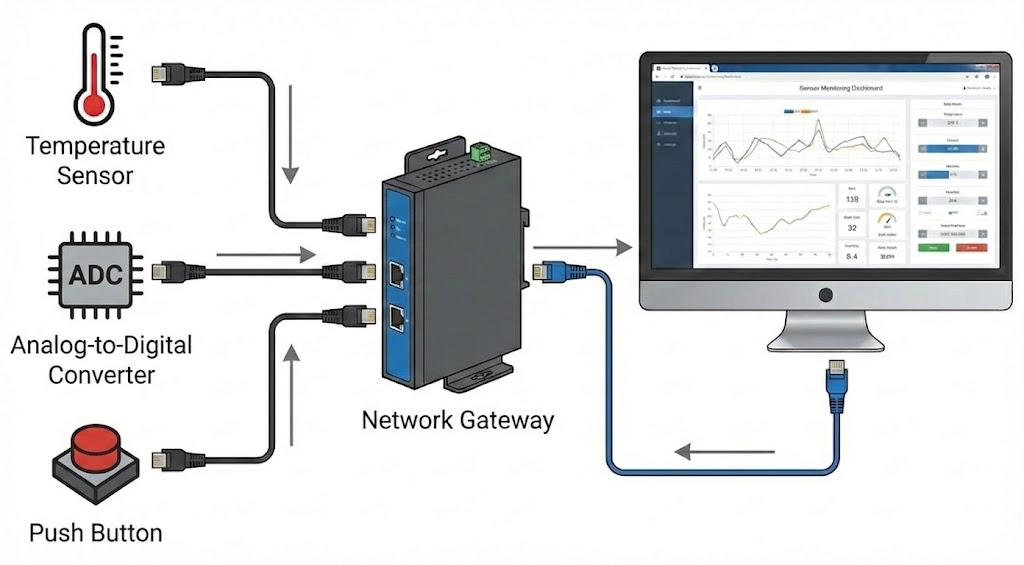
\includegraphics[width = 0.8\textwidth]{media/akshayintro1.png}
\caption{Measurement Network Gateway Interconnection}
\label{fig-akshay1}
\end{figure}

	
\subsection{System Architecture \& Design}
The system is engineered as a distributed network management gateway, designed to facilitate swift and reliable telemetry communication across remote nodes. Operating on a client-server paradigm, the core gateway application is deployed on a Linux operating system running atop the Xilinx Zynq-7000 SoC (ZedBoard), granting it direct interaction with physical hardware components. Conversely, the remote client features a graphical platform utilized to continuously monitor real-time data streams and dynamically configure the distant sensor devices over the TCP/IP network.

\begin{figure}[H]
\centering 
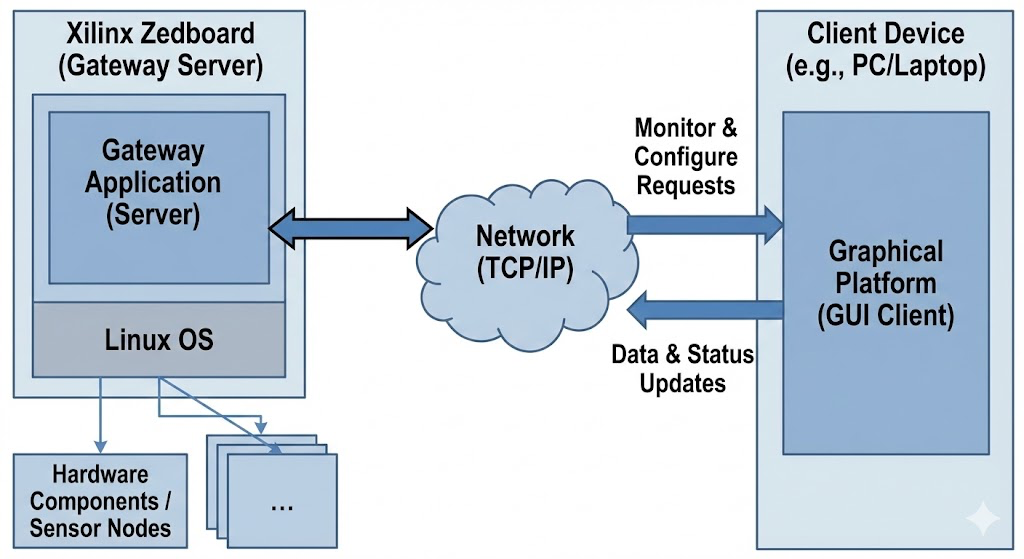
\includegraphics[width = 0.8\textwidth]{media/akshayintro5.png}
\caption{Server-client approach between devices}
\label{fig-akshay2}
\end{figure}
	
	
Concurrent Producer-Consumer Model - To guarantee that data acquisition
remains deterministic and immune to network latency, the internal system
architecture is explicitly built upon a concurrent Producer-Consumer model.
The core of the system is the Sensor Thread, which executes a precise timing
loop to poll hardware peripherals through a custom Linux kernel driver
(\texttt{/dev/meascdd}). By utilizing high-resolution sleep timers and direct
register access, this thread ensures that temperature and analog signals are
sampled at exact user-defined intervals without drift. To achieve this across
multiple independent sensors, the thread employs an "Earliest Deadline First"
scheduling algorithm. It continuously calculates the exact microsecond the
next sensor sample is due and safely yields CPU cycles using \texttt{usleep()}
until that specific deadline is reached.

Decoupling and Shared Memory - To decouple the strict timing requirements of
the hardware from the unpredictable nature of network communication, a
thread-safe Ring Buffer is employed as an intermediate storage mechanism.
Protected by Mutex (Mutual Exclusion) locks, this circular buffer allows the
Sensor Thread to continuously push new data points without blocking, while the
Server Thread (the Consumer) asynchronously retrieves them for transmission.
Crucially, this memory sharing is further optimized using POSIX Condition
Variables (\texttt{pthread\_cond\_t}). Instead of the Server Thread
continuously polling the buffer and wasting CPU resources, it enters a deep
zero-CPU sleep state when the buffer is empty. The exact microsecond the
Sensor Thread commits a new reading to memory, it issues a signal that
instantaneously wakes the Server Thread to batch and transmit the data.

Network Communication and Stability - The Server Thread manages the network
interface, listening on Port 50012 for incoming TCP connections. It handles a
custom command protocol (e.g., \texttt{start}, \texttt{stop},
\texttt{configure}), allowing remote users to dynamically adjust sampling
rates or pause the stream. For instance, the \texttt{configure} command parses
space-delimited string payloads to dynamically update the independent polling
frequencies of the ADC, temperature, and switch components on the fly.

This separation of concerns—isolating the hardware logic from the
communication logic guarantees system stability. Even if the network
connection drops or the client becomes unresponsive, the sensor data
acquisition continues uninterrupted, preventing data loss or system hangs.
Ultimately, this project demonstrates a scalable, industrial-grade solution
for embedded data aggregation, showcasing the effective use of POSIX threads,
event-driven synchronization primitives, and low-level driver interaction on
an embedded Linux platform.

The project is divided into hardware and software parts that fully integrate
later to make project working. In Hardware components, Zynq-7000 ZedBoard,
MAX31865 RTD-to-Digital converter, PmodAD1, RTD-Based Temperature measurement.
On the other hand, Linux kernel is built to integrate hardware information into
the software providing a platform to run the application. It uses ARM core
processors of Xilinx's Zedboard to operate Linux OS. Further, a Remote screen
or Graphical user interface is developed which communicates with the hardware
using Transmission Control Protocol (TCP/IP).


%


\subsection{Architectural Overview \& Userspace Bridging}
The module serves as the critical translation layer between the
high-level multithreaded server logic and the physical hardware of the
Xilinx ZedBoard. Because Linux strictly separates userspace applications
from physical hardware memory, this module acts as a secure bridge
utilizing standard POSIX file operations. By hiding complex
bit-shifting, SPI polling loops, and timeout safeguards behind simple
functions like \texttt{TempRead()} and \texttt{GetADC()}, it allows the
higher-level multithreaded architecture to remain clean, fast, and
entirely focused on timing and network transmission. The
\texttt{sensor\_read.c} file is a robust, fault-tolerant module.

\begin{minted}[bgcolor = lightgray, tabsize = 4, breaklines]{c}
    #include <fcntl.h>
    #include <unistd.h>
    #include "measdev.h"
    #include "sensor_read.h"
    MeasObj_struct TF_Obj_Snd, TF_Obj_Rcv;
\end{minted}


\begin{itemize}
    \item \textbf{Communication Struct (\texttt{MeasObj\_struct})}: The
          application cannot read physical memory addresses directly.
          Instead, it packs commands into \texttt{TF\_Obj\_Snd} (Transmit)
          and pushes them into the file descriptor \texttt{fd} pointing to
          the custom kernel driver (\texttt{/dev/meascdd}). The hardware
          response is then retrieved via \texttt{TF\_Obj\_Rcv}.

    \item \textbf{Modularity}: By hiding complex bit-shifting and SPI
          polling loops inside this module, the main sensor thread remains
          clean, lightweight, and hardware-agnostic.
\end{itemize}

\subsubsection{Low-Level SPI Protocol Management}
Interacting with the MAX31865 temperature chip requires precise,
timing-aware SPI bus transactions. The functions \texttt{MaxRead()} and
\texttt{MaxWrite()} are engineered to handle the physical delays of
hardware communication safely using strict polling loops and timeout
safeguards.

\subsubsection*{The MaxRead Function}
\begin{minted}[bgcolor = lightgray, tabsize = 4, breaklines]{c}
unsigned int MaxRead(int fd, unsigned int mreg)
{
    unsigned int xdata;
    int k;

    mreg <<= 8;
    TF_Obj_Snd.rnum = 1;
    TF_Obj_Snd.rvalue = mreg;
    write(fd, &TF_Obj_Snd, MEASOBJ_SIZE);
\end{minted}

\subsubsection*{Command Preparation \& Transfer: }
The target register address is shifted left by 8 bits (\texttt{mreg <<= 8}) and pushed to the driver (\texttt{rnum = 1}).
\begin{minted}[bgcolor = lightgray, tabsize = 4, breaklines]{c}
    k = 0;
    xdata = 0xc0000000;
    do {
        TF_Obj_Snd.rnum = REGNUM_ID;
        TF_Obj_Snd.rvalue = 1;
        write(fd, &TF_Obj_Snd, MEASOBJ_SIZE);
        k++;
        read(fd, &TF_Obj_Rcv, MEASOBJ_SIZE); // Read response from LKM
        xdata = TF_Obj_Rcv.rvalue;
    } while (((xdata & 0x01) == 0) && (k < 1000));
\end{minted}

\subsubsection*{The Polling State Machine \& Timeout: }
The code enters a strict \texttt{do-while} loop, querying the driver
for a status update. It checks whether the hardware is ready by
inspecting the lowest bit (\texttt{xdata \& 0x01}). The loop is capped
at \texttt{k < 1000} iterations to prevent system freezes if the
physical wire is disconnected.

\begin{minted}[bgcolor = lightgray, tabsize = 4, breaklines]{c}
    if (k >= 1000) {
        printf(" *** MaxRead timeout.");
    } else {
        TF_Obj_Snd.rnum = REGNUM_ID;
        TF_Obj_Snd.rvalue = 2;
        write(fd, &TF_Obj_Snd, MEASOBJ_SIZE);
        read(fd, &TF_Obj_Rcv, MEASOBJ_SIZE); // Read response from LKM
        xdata = TF_Obj_Rcv.rvalue;
        xdata &= 0x0ff;
    }
    return xdata;
}
\end{minted}

\subsubsection*{Data Extraction: }
Once ready, it reads the final value and masks it (xdata \&= 0x0ff) to ensure a clean 8-bit payload.

\subsubsection{The MaxWrite Function}
To signal a write operation over SPI, the highest bit of the register
address is set to \texttt{1} (\texttt{mreg |= 0x080}).

\begin{minted}[bgcolor = lightgray, tabsize = 4, breaklines]{c}
void MaxWrite(int fd, unsigned int mreg, unsigned int msend)
{
    unsigned int transm_data, xdata;
    int k;

    mreg |= 0x080;
    transm_data = (mreg << 8) | (msend & 0x0ff);
    TF_Obj_Snd.rnum = 1;
    TF_Obj_Snd.rvalue = transm_data;
    write(fd, &TF_Obj_Snd, MEASOBJ_SIZE);
\end{minted}

\subsubsection*{Payload Construction: }
The 16-bit payload combines the register address and the data byte:
\texttt{(mreg << 8) | (msend \& 0x0ff)}. Identical to \texttt{MaxRead()},
it uses the 1000-iteration polling loop to guarantee the write command
was physically clocked into the sensor.

\begin{minted}[bgcolor = lightgray, tabsize = 4, breaklines]{c}
     k = 0;
    xdata = 0xc0000000;
    do {
        TF_Obj_Snd.rnum = REGNUM_ID;
        TF_Obj_Snd.rvalue = 1;
        write(fd, &TF_Obj_Snd, MEASOBJ_SIZE);
        k++;
        read(fd, &TF_Obj_Rcv, MEASOBJ_SIZE); // Read response from LKM
        xdata = TF_Obj_Rcv.rvalue;
    } while (((xdata & 0x01) == 0) && (k < 1000));
    
    if (k >= 1000) {
        printf(" *** MaxWrite timeout.");
    }
}
\end{minted}

\subsubsection*{MAX31865 Temperature Sensor API}
This section wraps the complex \texttt{MaxRead()} and \texttt{MaxWrite()}
logic into three simple lifecycle functions tailored specifically for the
MAX31865 RTD-to-Digital converter.

\paragraph{Initialization (TempPowerUp): }
Writes the hex value \texttt{0xC1} to the configuration register. This turns on VBIAS, enables Auto-Conversion mode, and enables the 50Hz hardware noise rejection filter. A calculated \texttt{usleep(75000)} allows the analog circuitry 75ms to settle.
\begin{minted}[bgcolor = lightgray, tabsize = 4, breaklines]{c}
int TempPowerUp(int fd)
{
    ssize_t ret;

    TF_Obj_Snd.rnum   = 0;
    TF_Obj_Snd.rvalue = 0x022;
    ret = write(fd, &TF_Obj_Snd, MEASOBJ_SIZE);
    if (ret < 0) { perror("Sensor Initialization Failed"); return -1; }

    MaxWrite(fd, 0x00, 0xC1);   // VBIAS=ON, AutoConv=ON, 2-wire, 50Hz
    usleep(75 * 1000);           // 10ms VBIAS settle + 65ms first conversion
    printf("MAX31865 powered up in auto-conversion mode\n");
    return 1;
}
\end{minted}



\paragraph{Data Retrieval (TempRead): }
Fetches the Most Significant Byte (MSB) and Least Significant Byte (LSB). It evaluates \texttt{if (lsb \& 0x01)} to detect hardware faults (like a broken wire) to prevent broadcasting false data. If valid, the 16-bit integer is reassembled and shifted right by 1 (\texttt{>> 1}) to discard the fault bit, isolating the true 15-bit ADC count.
\begin{minted}[bgcolor = lightgray, tabsize = 4, breaklines]{c}
int TempRead(int fd, int *output_raw)
{
    unsigned int msb = MaxRead(fd, 0x01);
    unsigned int lsb = MaxRead(fd, 0x02);

    if (lsb & 0x01) {
        printf("MAX31865 fault: 0x%02X\n", MaxRead(fd, 0x07));
        return -1;
    }

    *output_raw = (int)((((msb & 0xFF) << 8) | (lsb & 0xFF)) >> 1);
    return 1;
}
\end{minted}


\paragraph{Safe Termination (TempShutdown): }
Writes \texttt{0x01} to disable VBIAS and save power during system shutdown.
\begin{minted}[bgcolor = lightgray, tabsize = 4, breaklines]{c}
void TempShutdown(int fd)
{
    MaxWrite(fd, 0x00, 0x01);
    printf("MAX31865 powered down\n");
}
\end{minted}

\subsubsection{Dual-Channel Analog-to-Digital (ADC) Processing}
The GetADC function communicates with the ZedBoard's ADC peripherals, handling two separate voltage channels simultaneously.
\begin{minted}[bgcolor = lightgray, tabsize = 4, breaklines]{c}
void GetADC(int fd, unsigned int *adc0_out, unsigned int *adc1_out)
{
    int  ccount;
    unsigned int xstatus, adc0, adc1;
    TF_Obj_Snd.rnum = 4;        // start conversion
    TF_Obj_Snd.rvalue = 0;
    write(fd, &TF_Obj_Snd, MEASOBJ_SIZE);
    ccount = 0;
    
    do {
        ccount++;
        read(fd, &TF_Obj_Rcv, MEASOBJ_SIZE);        // Read response from LKM
        xstatus = TF_Obj_Rcv.rvalue;
    } while ((xstatus == 0) && (ccount < 10000000));
\end{minted}

\paragraph{Trigger and Wait: }
Writes a \texttt{0} to \texttt{rnum = 4} to signal the FPGA to sample analog voltages. An extended polling loop (\texttt{ccount < 10000000}) provides the hardware ample time to charge its internal capacitors and complete the conversion.
\begin{minted}[bgcolor = lightgray, tabsize = 4, breaklines]{c}
       TF_Obj_Snd.rnum = REGNUM_ID;
    TF_Obj_Snd.rvalue = 5;      // ADC status register
    write(fd, &TF_Obj_Snd, MEASOBJ_SIZE);
    read(fd, &TF_Obj_Rcv, MEASOBJ_SIZE);        // Read response from LKM
    
    adc1 = TF_Obj_Rcv.rvalue;
    adc0 = adc1 & 0x0fff;
    adc1 >>= 16;
    *adc0_out = adc0;
    *adc1_out = adc1;
}
\end{minted}

\paragraph{Bitwise Separation: }
The hardware returns a highly optimized 32-bit package containing both readings.
\begin{itemize}
    \item \textbf{ADC0 Extraction:} Applies a bitwise AND mask (\texttt{adc1 \& 0x0fff}) to isolate the lowest 12 bits (values 0--4095).
    \item \textbf{ADC1 Extraction:} Applies a bitwise right-shift (\texttt{adc1 >>= 16}) to push the upper 12 bits down to the bottom, safely separating the second reading.
\end{itemize}

\subsubsection{Digital I/O (Switches, Buttons, and LEDs)}
This section maps the physical user interface of the ZedBoard directly into the software.

\paragraph{Switch Acquisition (ReadSwitch): }
Queries the main status register. Applying an \texttt{\& 0xff} (Binary: \texttt{1111 1111}) mask to the 32-bit return value instantly zeroes out irrelevant upper bits, isolating the exact ON/OFF states of the 8 physical sliding switches.

\begin{minted}[bgcolor = lightgray, tabsize = 4, breaklines]{c}
    unsigned int ReadSwitch(int fd)
{
    TF_Obj_Snd.rnum = REGNUM_ID;
    TF_Obj_Snd.rvalue = 0;
    write(fd, &TF_Obj_Snd, MEASOBJ_SIZE);
    read(fd, &TF_Obj_Rcv, MEASOBJ_SIZE);
    
    return (TF_Obj_Rcv.rvalue) & 0xff;
}
\end{minted}

\subsubsection*{Push Button Acquisition (ReadButton): }
Queries the exact same register but shifts the result right by 8 bits (\texttt{>> 8}). Because there are only 5 push buttons, it applies a strict \texttt{\& 0x1f} (Binary: \texttt{0001 1111}) mask to isolate just those 5 states.
\begin{minted}[bgcolor=lightgray, tabsize=4, breaklines]{c}
unsigned int ReadButton(int fd)
{
    TF_Obj_Snd.rnum = REGNUM_ID;
    TF_Obj_Snd.rvalue = 0;
    write(fd, &TF_Obj_Snd, MEASOBJ_SIZE);
    read(fd, &TF_Obj_Rcv, MEASOBJ_SIZE);

    return ((TF_Obj_Rcv.rvalue) >> 8) & 0x1f;
}
\end{minted}

\subsubsection*{LED Control (LedWrite): }
Pushes a standard 8-bit hex payload to \texttt{rnum = 0}. The FPGA hardware interprets this payload and instantly illuminates the corresponding sequence of the 8 onboard yellow LEDs, providing real-time visual feedback.

\begin{minted}[bgcolor=lightgray, tabsize=4, breaklines]{c}
void LedWrite(int fd, uint8_t LED_hex_Value)
{
    ssize_t ret;
    TF_Obj_Snd.rnum   = 0;       // write reg0 (lower 8 bits = uzLED)
    TF_Obj_Snd.rvalue = (unsigned int)LED_hex_Value;
    ret = write(fd, &TF_Obj_Snd, MEASOBJ_SIZE);
    if (ret < 0) perror("LED writing failed");
}
\end{minted}








\clearpage 


\section{Network Communication}
\subsection{Transmission Control Protocol (TCP)}
It is one of the most fundamental protocols of the internet. If the internet is a massive highway system, IP (Internet Protocol) is the GPS routing the trucks, and TCP is the logistics company ensuring every single package arrives intact, in the correct order, and confirming delivery with the sender.
The Transmission Control Protocol (TCP) is a foundational communication protocol of the modern internet. While the Internet Protocol (IP) manages the addressing and routing of packets across disparate networks, TCP operates at the transport layer to ensure the reliable, ordered, and error-checked delivery of data streams between applications communicating over an IP network.

\subsection{Core Characteristics of TCP}
TCP was specifically engineered to mitigate the inherent unreliability of physical network infrastructure, where latency, packet loss, and hardware limitations are commonplace. By operating transparently over this variable underlying layer, TCP provides applications with a robust and dependable communication channel.
\begin{itemize}
\item \textbf{Connection-Oriented:} Prior to any data transmission, TCP establishes a formal session between endpoints using a protocol known as the three-way handshake. This synchronizes sequence numbers and operational parameters between the client and server.
\item \textbf{Reliable Delivery:} TCP employs a strict system of acknowledgments and timeouts. If a transmitted segment is not acknowledged by the receiver within a specified timeframe, TCP assumes the packet was lost and automatically retransmits the data, guaranteeing complete delivery.
\item \textbf{In-Order Delivery:} Because individual IP packets may traverse different network paths and arrive out of sequence, TCP affixes a sequence number to each segment. This allows the receiving network stack to reassemble the payload in the precise order it was originally transmitted.
\item \textbf{Error Checking:} Each TCP segment includes a cryptographic checksum in its header. The receiver independently calculates the checksum of the incoming data and compares it to this field to detect bit-level corruption that may have occurred during transit.
\item \textbf{Flow Control:} To prevent a high-bandwidth sender from overwhelming a receiver with limited processing capacity or memory, TCP utilizes a sliding window mechanism. The receiver continuously advertises its available buffer space, dictating the maximum volume of unacknowledged data the sender is permitted to transmit at any given moment.
\item \textbf{Congestion Control:} TCP implements advanced algorithms to detect network-wide congestion (typically inferred from dropped packets or delayed acknowledgments). Upon detecting network saturation, the protocol dynamically throttles its transmission rate to alleviate strain on intermediary routers and prevent systemic network collapse.
\end{itemize}



\clearpage
\subsection{TCP Server-Client Connection}
\begin{figure}[H]
\centering 
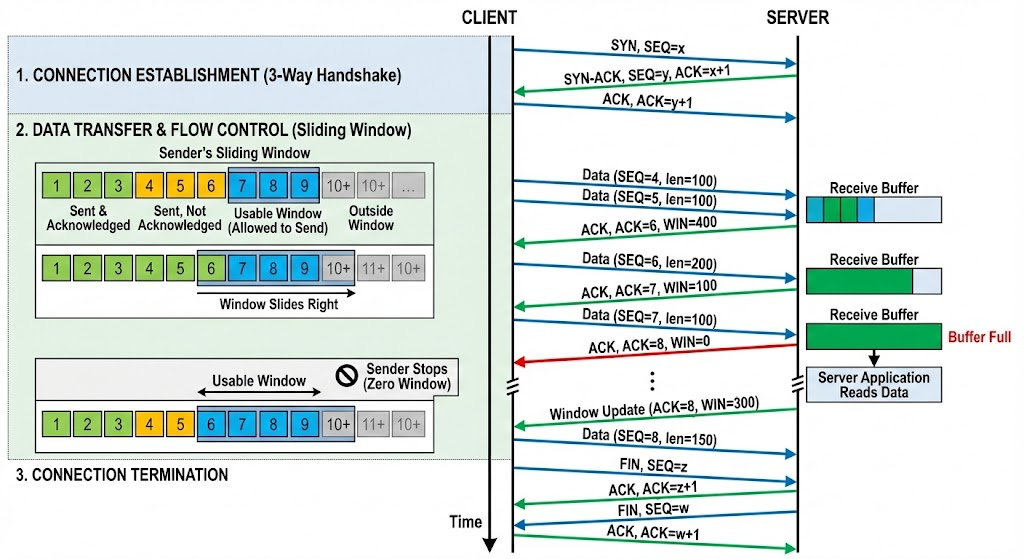
\includegraphics[width = 0.9\textwidth]{media/akshayintro8.png}
\caption{TCP Client-Server setup connection}
\label{fig-akshyintro3}
\end{figure}
	
The Transmission Control Protocol (TCP) provides the foundation for reliable network communication. In the context of your embedded gateway system, this protocol governs the stable, continuous streaming of sensor data from the server to the client dashboard. The TCP connection lifecycle is structured around three primary phases:
	

\textbf{1. Connection Establishment :} Prior to any data transmission, the client and server must synchronize their connection states. The client initiates this process by transmitting a SYN (Synchronize) packet containing an initial sequence number. The server allocates the necessary resources and responds with a SYN-ACK packet, which the client then formally acknowledges (ACK). This establishes a secure, bidirectional communication channel.

\textbf{2. Data Transfer and Flow Control :} To prevent high-speed data streams from overwhelming the receiving system's memory, TCP employs a dynamic "Sliding Window" protocol.

\begin{itemize}
\item Buffer Management: The receiving server allocates a finite memory buffer for incoming data. With every acknowledgment (ACK) it sends back to the client, it also advertises its current available buffer capacity using the Window Size (WIN) parameter.
\item State Tracking: The sender categorizes data into strict states (acknowledged, in-transit, permitted to send, and blocked) and restricts its transmission output to fit within the receiver's advertised window.
\item The "Zero Window" State: If the receiver's buffer reaches maximum capacity, it broadcasts a WIN=0. To prevent data loss, the sender immediately halts transmission. Once the receiving application processes the buffered data, the receiver issues a Window Update with a non-zero value, allowing transmission to resume.
\end{itemize}

\textbf{3. Connection Termination:} Upon completing the data transfer, the session is gracefully dismantled to ensure no in-transit data is corrupted or lost. Both the client and server perform a reciprocal exchange of FIN (Finish) and ACK packets. Once both sides have confirmed termination, the connection is formally closed, and the operating system releases the associated ports and memory resources.

\fancyhead[L]{Multithreading in MNG (Akshay Vastrad 42723)}
\section{Multithreading}
Multithreading is a term used for the techniques or procedures in which multiple applications can run simultaneously. These procedures could be hardware or software based. It helps in improving the performance by increasing the computing speed as more than one application can run at the same time in parallel. The application must be ready for this operation and can be divided into meaningful threads. An essential interaction between hardware and software is required before applying multithreading.
A thread has its own register, counter, and stack and is a flow to execution through the process code. Thread is a type of lightweight process. Threads provide a way to improve application performance through the parallel operation. Each thread performs exactly one routine, and no thread exists out of the routine. Every thread follows a distinct flow of control.

\begin{figure}[H]
\centering 
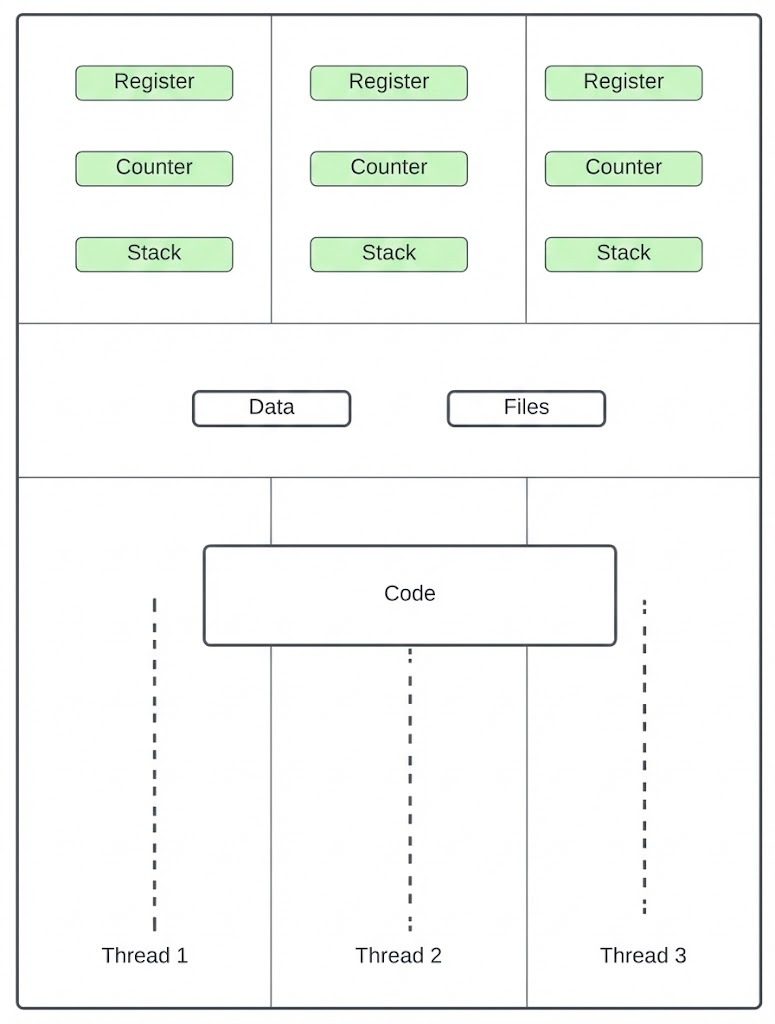
\includegraphics[scale = 0.4]{media/akshayintro3.png}
\caption{text}
\label{fig-akshayintro3}
\end{figure}




To achieve concurrent data acquisition and network transmission, the project utilizes the POSIX Threads (pthread) library. This library provides the primitives required to manage parallel execution paths within the Linux userspace. The specific functions utilized in this project are detailed below:

\subsection{Thread Management}
\begin{itemize}
    \item \texttt{pthread\_create( )}: Create a new thread
   	\begin{minted}[bgcolor = lightgray, tabsize = 4, breaklines]{c}
   	int pthread_create(pthread_t *thread, const pthread_attr_t *attr, void *(*start_routine)(void *), void *arg);
   	\end{minted}
    This function is the entry point for parallel execution. In this project,
    it is used in \texttt{main()} to spawn two critical worker threads: the
    Sensor Thread and the Server Thread. It takes the thread ID pointer,
    thread attributes (passed as \texttt{NULL} for default settings), and the
    function to execute (e.g., \texttt{sensor\_thread\_function}). A return
    value of zero indicates successful creation.

    \item \texttt{pthread\_join( )}: Wait for thread termination
    \begin{minted}[bgcolor = lightgray, tabsize = 4, breaklines]{c}
    int pthread_join(pthread_t thread, void **retval);
    \end{minted}
    This function is used by the main thread to wait for the worker threads to
    finish their execution. It acts as a blocking mechanism; the main program
    will not exit until the specified thread terminates. In this system, it
    ensures the application remains active and does not shut down prematurely
    while the sensors are still monitoring.
\end{itemize}

\subsection{Synchronization (Mutexes)}
Since multiple threads attempt to access shared resources, specifically the Ring Buffer for data storage and the Configuration Structure for settings synchronization is mandatory to prevent data corruption (Race Conditions). We utilize Mutexes (Mutual Exclusion objects) to enforce safe access.

\begin{itemize}
    \item \texttt{pthread\_mutex\_init( )}: Initialize the mutex
    \begin{minted}[bgcolor = lightgray, tabsize = 4, breaklines]{c}
int pthread_mutex_init(pthread_mutex_t *mutex, const pthread_mutexattr_t *attr);
    \end{minted}
    Called at the start of the program, this prepares the mutex object for
    use. It sets the mutex to an unlocked state, making it ready to manage
    resource contention.

    \item \texttt{pthread\_mutex\_lock( )}: Acquire the lock
    \begin{minted}[bgcolor = lightgray, tabsize = 4, breaklines]{c}
int pthread_mutex_lock(pthread_mutex_t *mutex);
    \end{minted}
    Before a thread can read or write to the shared Ring Buffer, it calls this
    function. If the buffer is currently free, the thread locks it and
    proceeds. However, if the other thread is already holding the lock, the
    calling thread is put to sleep (blocked) until the mutex becomes
    available. This guarantees atomic access to the data.

    \item \texttt{pthread\_mutex\_unlock( )}: Release the lock
    \begin{minted}[bgcolor = lightgray, tabsize = 4, breaklines]{c}
int pthread_mutex_unlock(pthread_mutex_t *mutex);
    \end{minted}
    Immediately after the data transfer is complete, the thread calls this
    function to release the mutex. This allows the waiting thread to wake up
    and access the shared resource.

    \item \texttt{pthread\_mutex\_destroy( )}: Clean up resources
    \begin{minted}[bgcolor = lightgray, tabsize = 4, breaklines]{c}
int pthread_mutex_destroy(pthread_mutex_t *mutex);
    \end{minted}
    Used during the system shutdown phase, this function destroys the mutex
    object, freeing any system resources associated with the lock mechanism.
\end{itemize}


\subsection{Sensor Thread}
This thread is exclusively responsible for precision timing and hardware data
acquisition. By offloading this workload, the main application is free to
handle TCP network communication and high-level client command logic, while
the sensor thread manages the low-level protocols required to extract accurate
temperature, ADC, and digital I/O readings.

The thread attempts to open the specific Linux device driver
(\texttt{/dev/meascdd}); if the physical hardware is not present, it
automatically falls back to a `Simulation Mode' that generates realistic sine
waves and dummy data. Inside its continuous execution loop, it calculates the
exact microsecond when the next sample is due for each individual sensor
(e.g., \texttt{next\_temp\_time}, \texttt{next\_adc0\_time}) using an Earliest
Deadline First approach rather than relying on fixed sleep intervals. When a
sensor's precise deadline is reached, the thread calls the specific reading
function (such as \texttt{TempRead} or \texttt{GetADC}) which interacts with
the hardware via a safe hardware-polling loop and then pushes the acquired data
and a microsecond timestamp into the thread-safe Ring Buffer to be processed
by the server thread.

This report details the architectural design, lifecycle management, data
acquisition strategies, and the synchronization mechanisms that constitute the
sensor thread.


\begin{figure}[H]
\centering 
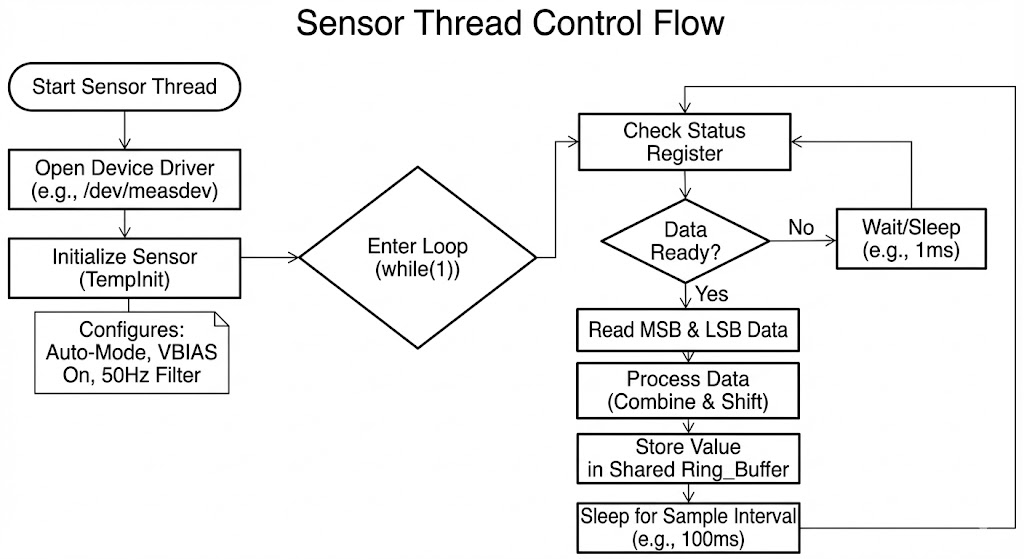
\includegraphics[width = 0.9\textwidth]{media/akshayintro7.png}
\caption{Flowchart Sensor thread control flow}
\label{fig-alshay7}
\end{figure}

The software architecture adopted for this project is a layered model designed
to abstract the complexities of hardware interaction from the application
logic. At the lowest level lies the physical hardware: the MAX31865 sensor
chip connected via SPI to the FPGA fabric of the Zynq SoC. Above this sits
the Linux Kernel Module (LKM), a device driver that exposes the hardware to
the operating system as a character device file, typically located at
\texttt{/dev/measdev}.

The Sensor Thread operates in the userspace layer, acting as the Hardware
Abstraction Layer (HAL). It communicates with the kernel driver using standard
POSIX file operations—specifically \texttt{open()}, \texttt{write()}, and
\texttt{read()}. This design choice is significant because it allows the
application to remain portable and relatively simple; the complex timing and
electrical signg required by the SPI bus are handled by the kernel driver
and the FPGA logic. The sensor thread's role is to construct the correct
command packets defined as \texttt{TF\_Obj\_Snd} for sending and
\texttt{TF\_Obj\_Rcv} for receiving that tell the driver which register to
access and what value to write. This transactional protocol ensures that the
application has fine-grained control over the sensor configuration without
needing direct access to physical memory addresses.

The lifecycle of the sensor thread is distinct from the main application,
following a rigorous sequence of initialization, execution, and termination.
Upon creation, the thread's first responsibility is to establish a
communication channel with the hardware. It does this by obtaining a file
descriptor to the device driver. This descriptor serves as a handle for all
subsequent interactions; if the driver cannot be opened, the thread must
handle this failure gracefully, typically by logging an error and exiting, as
the system cannot function without access to the sensor.

Once the connection is established, the thread enters the initialization
phase. The MAX31865 sensor defaults to a low-power ``sleep'' state upon
power-up and must be explicitly configured before it can perform any
conversions. The sensor thread executes a function, which sends a specific
sequence of commands to the sensor's Configuration Register (Address
\texttt{0x00}). The first command sets the VBIAS bit (Bit 7), which turns on
the DC bias voltage required to measure the resistance of the PT100 probe.
Without this voltage, the sensor would read effectively zero resistance. The
second critical command configures the internal digital filter. In industrial
environments, electrical noise from 50Hz mains power lines can couple into the
sensor wires, corrupting the sensitive analog measurements. The thread writes a
command to enable the 50Hz rejection filter, instructing the MAX31865 to
average its samples in a way that mathematically cancels out this specific
frequency interference. Finally, the thread sets the ``Auto Conversion'' bit,
switching the sensor from ``One-Shot'' mode to ``Continuous'' mode, where it
autonomously performs conversions in the background.


\begin{figure}[H]
\centering 
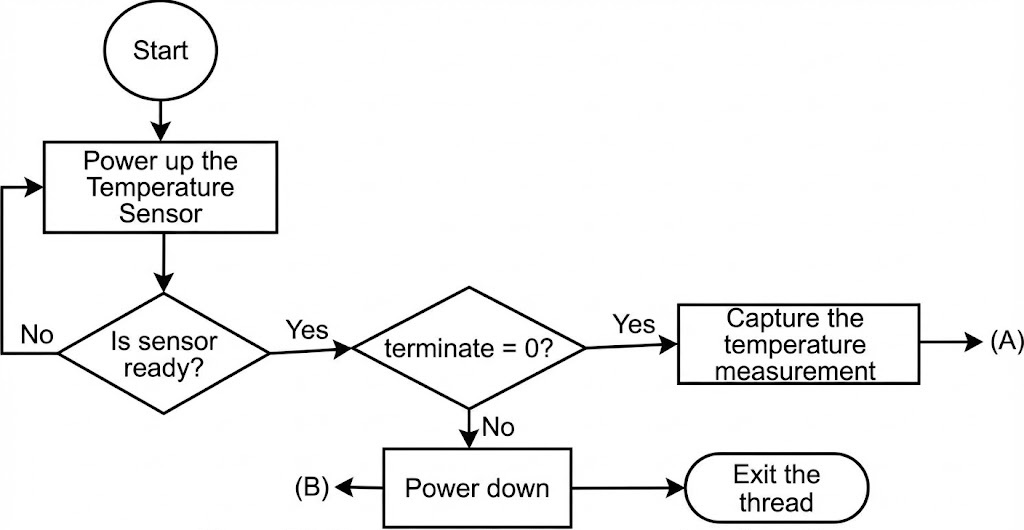
\includegraphics[width = 0.9\textwidth]{media/akshayintro2.png}
\caption{Flow chart of Temperature sensor thread}
\label{fig-akshayintro6}
\end{figure}

The provided flowchart illustrates the execution sequence for the temperature
sensor thread within the data acquisition system. The process begins at the
``Start'' state, immediately proceeding to a block instructing the system to
``Power up the Temperature Sensor''. Because the physical hardware requires a
brief period to initialize, the system enters a validation loop, querying the
condition ``Is sensor ready?''. If the sensor is not yet responsive, the loop
cycles back continuously until the hardware confirms its readiness.

Once the temperature sensor is fully operational, the thread evaluates a
critical control flag by asking if ``terminate = 0?''. This condition
determines whether the thread should continue its normal operation or begin a
shutdown sequence. If the flag indicates that no termination has been requested
(evaluating to ``Yes''), the thread proceeds to ``Capture the temperature
measurement''. After the data is successfully captured, the flow transitions
to a subsequent processing stage, which is indicated by the external connector
(A).

Alternatively, if a termination signal has been detected, the system halts any
further data measurements. It safely transitions to a shutdown routine to
``Power down'' the hardware components. After safely powering down the sensor,
the execution reaches its final conclusion at ``Exit the thread''.
Additionally, this secure power-down and exit sequence can also be triggered
via an external path labeled with connector (B).

\clearpage 
\subsection{ADC Sensor Thread}
\begin{figure}[H]
\centering 
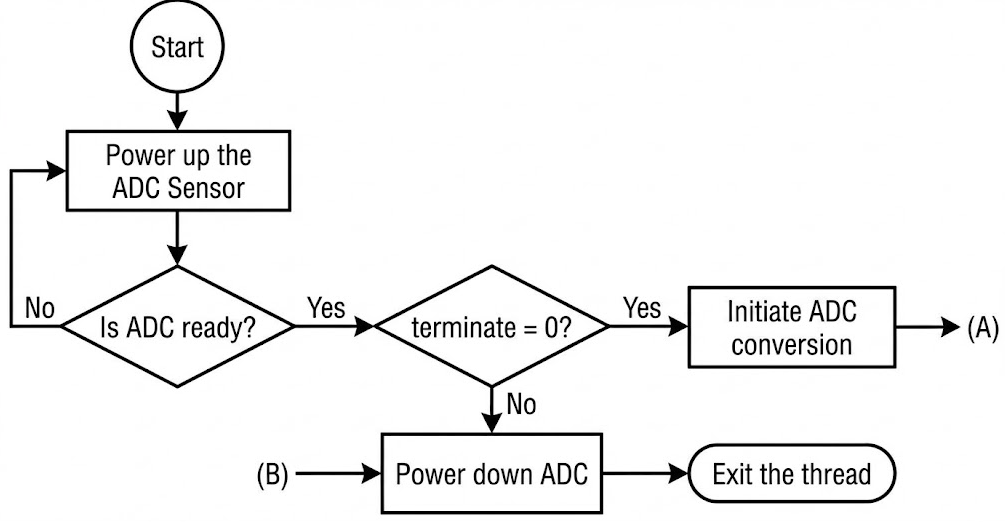
\includegraphics[width = 0.8\textwidth]{media/akshayintro6.png}
\caption{Flow chart of ADC sensor thread}
\label{fig-akshay6}
\end{figure}

The provided flowchart outlines the execution, hardware polling, and
termination logic for the Analog-to-Digital Converter (ADC) sampling sequence
within the embedded system's unified sensor thread.

The sequence begins by evaluating a core control condition, checking if the
thread's termination flag is equal to 0. This acts as the main execution
safeguard at the start of the thread's continuous loop. If the condition is
true, the system proceeds to issue a `Request Conversion' command to the ADC
hardware. Because hardware peripherals require time to sample analog voltage,
the system enters a polling loop that repeatedly asks, `Is the ADC ready?'.
If the hardware is not yet responsive, the loop continuously cycles back
safely yielding CPU time until a positive status confirmation is received from
the sensor driver.

Once the ADC confirms it has completed the conversion, the system reads the
raw data registers before moving to a subsequent processing and buffering
phase denoted by Connector (A).

Conversely, if the system receives a termination request, it immediately
aborts any further data sampling. It transitions directly to a safety sequence
to cleanly power down associated hardware and close the device file descriptors
before ultimately concluding with `Exit the thread'. Furthermore, this cleanup
block can also be accessed via an external path labeled with Connector (B),
ensuring that the hardware is always safely deactivated prior to thread
closure.

\subsection{Push Button Data Acquisition Strategy}
This system integrates the Push Button interface directly into the centralized Sensor Thread. This design choice eliminates the overhead of context switching between multiple threads and ensures deterministic sampling synchronization with the other sensors.

This flowchart illustrates the specific execution steps for acquiring data
from the digital Push Button sensors. It details the sequence of operations
that occur once the system determines it is time to sample the buttons.

\begin{itemize}
    \item \textbf{Capture Measurement Time:} The process begins by recording
    the current system timestamp. This ensures the data is temporally accurate
    for later analysis.

    \item \textbf{Read Push Button Values:} The system accesses the hardware
    register to retrieve the current state of the buttons. This involves a
    low-level register read followed by bitwise operations (shifting and
    masking) to isolate the specific bits representing the button states.

    \item \textbf{Calculate Relative Time:} The system calculates the time
    difference between the current measurement and the initial system start
    time. This relative timestamp is used to reduce the data size required for
    storage.

    \item \textbf{Data Storage (FIFO):} The combined data packet containing
    the button state and the timestamp is copied into the Ring Buffer. This
    makes the data available for the Server Thread to transmit.

    \item \textbf{Exit/Loop:} The flow then proceeds to exit the specific task
    or loop back, waiting for the next scheduled sampling interval or a
    termination signal.
\end{itemize}

\begin{figure}[H]
\centering 
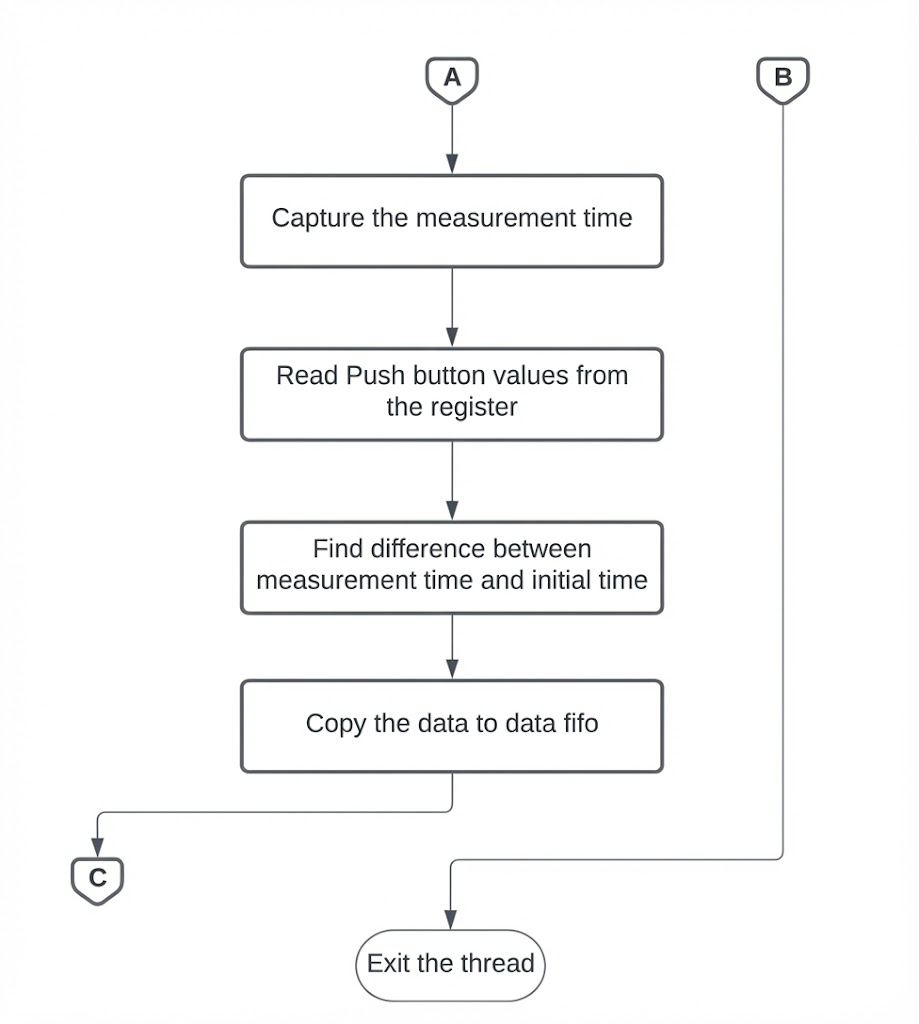
\includegraphics[width = 0.7\textwidth]{media/akshayintro4.png}
\caption{Flow chart of push button and switches thread}
\label{fig-akshay4}
\end{figure}

\subsection{The Data Acquisition Loop}
The core operational logic of the sensor thread is contained within an infinite while(1) loop. Rather than a simple continuous polling mechanism, this loop acts as a highly precise scheduler, utilizing an "Earliest Deadline First" approach to independently manage multiple sensors. When the exact microsecond deadline arrives for a temperature reading, the thread enters the hardware-specific data retrieval phase.

It initiates a 1-shot conversion and queries the sensor via the custom device driver. To prevent reading stale data while the MAX31865 completes its conversion, the thread inspects the status response from the hardware. It looks for a specific ready state, If the hardware is not yet ready, the thread performs a safe "busy wait," utilizing a function to yield the processor to the OS for 10 microseconds, preventing the CPU from spinning at 100\% utilization.

Once the ready state is confirmed, the thread proceeds to read the two data registers: the Most Significant Byte (MSB) at Address 1 and the Least Significant Byte (LSB) at Address 2. These two 8-bit values must be combined to form the complete 16-bit raw temperature reading. The thread performs this combination using bitwise operations, shifting the MSB left by 8 positions and performing a bitwise OR with the LSB.


\subsection{Data Processing and Fault Management}
The raw 16-bit integer retrieved from the MAX31865 is not yet a valid temperature value. The chip encodes fault information directly into the least significant bit (Bit 0) of the data word, acting as a flag to indicate hardware faults such as an open circuit or a short circuit in the RTD probe.

However, in this specific gateway architecture, the embedded C application prioritizes maximum throughput and deterministic latency. Therefore, the sensor thread does not locally perform the right-shift operations to isolate the fault bit, nor does it calculate the complex floating-point. Instead, the gateway acts as a transparent, high-speed conduit. It immediately pushes the pristine, raw 16-bit integer directly into the Ring Buffer. This architectural decision deliberately delegates the heavy mathematical conversions and fault-flag evaluations to the higher-level client dashboard receiving the TCP stream, keeping the embedded gateway incredibly lightweight, fast, and stable.

\subsection{Thread Synchronization and Shared Memory}
One of the most critical aspects of the sensor thread's design is how it safely shares data with the rest of the system. Since the sensor thread runs asynchronously to the TCP server thread, direct variable access would inevitably lead to "race conditions," where the server might read a corrupted value such as a mix of an old MSB and a new LSB.

To solve this, the system employs a robust Ring Buffer mechanism. The sensor thread acts as the "Producer," pushing valid, timestamped sensor readings into the buffer. The dedicated server thread acts as the "Consumer," reading these values to batch and transmit over the network.

This shared memory access is strictly protected by Mutex locks. The sensor thread locks the mutex before writing to the buffer and unlocks it immediately after, guaranteeing that the write operation is atomic and cannot be interrupted. Furthermore, the system implements advanced event-driven synchronization using a Condition Variable. Instead of the server thread wasting CPU cycles continuously polling the buffer to see if new data has arrived, it enters a deep sleep. The exact microsecond the sensor thread finishes a safe write, it fires a signal that instantly wakes the server thread to process the data.\\

\textbf{Client-Side Data Processing and GUI Visualization}

To maintain maximum throughput and minimize CPU overhead on the embedded
ZedBoard gateway, heavy mathematical computations and data unpacking are
deliberately offloaded to the remote client application. The client dashboard,
operating on a standard PC, connects to the gateway via a TCP socket and
continuously ingests the incoming byte stream.\\

\textbf{Data Parsing and Fault Masking}

Upon receiving the raw 16-bit integer generated by the MAX31865 sensor, the
client software first evaluates the least significant bit (Bit 0), which
serves as a hardware fault flag. If this bit is asserted (1), the client
triggers a graphical user interface (GUI) alert indicating a potential open
circuit or short circuit in the RTD probe. If the bit is clear (0), the
software performs a logical right-shift operation to discard the status bit,
successfully isolating the true 15-bit ADC count.\\

\textbf{Mathematical Conversion and Rendering}

The isolated raw integer represents the physical ratio of the RTD resistance
to the reference resistor. The client application then applies the
Callendar-Van Dusen equation to convert this raw resistance ratio into a
precise, human-readable floating-point temperature value in degrees Celsius.

Once processed, the temperature, alongside the decoded ADC voltages and
digital switch states, is pushed to the graphical platform. The dashboard
dynamically updates real-time plots and status indicators, providing operators with an intuitive, lag-free overview of the distant sensor nodes. This architectural decision keeps the embedded gateway incredibly lightweight and fast, while leveraging the superior processing power of the client PC for complex mathematics and UI rendering.

\subsection{Results and System Validation}
To verify the stability, concurrency, and network capabilities of the Measurement Network Gateway, extensive testing was conducted directly on the physical Xilinx Zynq-7000 SoC (ZedBoard).

The system's initialization sequence and hardware abstraction layer were thoroughly validated. The sensor thread successfully opened the custom /dev/meascdd Linux device driver and established SPI communication with the physical MAX31865 and ADC peripherals. The thread correctly transmitted the configuration bytes to enable the VBIAS and the 50Hz hardware noise filter. Monitoring the system confirmed that the continuous polling loop accurately retrieved real, fluctuating analog readings at the exact microsecond intervals dictated by the Earliest Deadline First scheduling algorithm.

The TCP/IP server thread was validated by connecting the custom graphical platform (GUI) to the gateway over the local network. The server successfully maintained the connection and accurately processed the custom command protocol (e.g., start, stop, configure). Once the stream was initiated, the GUI successfully ingested the raw 16-bit integers, masked the hardware fault bits, and applied the Callendar-Van Dusen equation. The dashboard dynamically updated the real-time plots and status indicators with accurate temperature and voltage readings, proving that the gateway's deliberate architectural choice to offload heavy mathematics to the client was highly effective.

Finally, the system was stress-tested to ensure the POSIX synchronization primitives functioned under continuous load. The concurrent Producer-Consumer architecture proved completely stable; the server thread managed network flow control and client communication without ever interrupting or blocking the underlying sensor data acquisition thread. The Mutex-protected Ring Buffer and POSIX Condition Variables successfully facilitated data exchange with zero dropped packets and near-zero CPU waste during idle states. Even when network latency was introduced or the client was intentionally disconnected, the sensor thread continued acquiring data uninterrupted, successfully preventing data loss and system hangs.

\subsection{Conclusion}
The Sensor Thread implementation detailed in this report represents a robust
and scalable solution for embedded data acquisition on the Xilinx ZedBoard
platform. By encapsulating hardware complexity within a dedicated,
high-performance thread, the system achieves a modular architecture where the
low-level intricacies of SPI communication and register manipulation are
completely abstracted from the high-level TCP server logic.

The thread manages the comprehensive lifecycle of multiple sensors. For the
temperature hardware, this ranges from the critical initialization sequence
which powers up the VBIAS and enables hardware-level noise filtering to the
precision-timed, continuous loops that retrieve the raw data. While the
hardware-to-thread interaction relies on a highly optimized, yielded polling
design (involving minor trade-offs in strict real-time determinism), the
thread-to-thread communication is fully event-driven. The implementation of a
Mutex-protected Ring Buffer paired with POSIX Condition Variables ensures safe,
reliable, and zero-CPU-waste data exchange with the main server application.

Ultimately, this architecture provides a highly stable and lightweight
foundation for industrial IoT monitoring systems, maintaining clear pathways
for future hardware-level optimizations via kernel-space wait queues and
hardware interrupt handling.





\newpage
\null 
\vfill
\begin{center}
\textbf{\large Mohammad Reza Rahimi (42756)}
\end{center}
\vfill
\fancyhead[L]{Introduction to Hardware in MNG (Mohammad Reza Rahimi 42756)}
\clearpage
	
\chapter{Introduction to Hardware in MNG}
\section{Introduction}
The Measurement Network Gateway (MNG) is one of the embedded measurement platform designed which to collect different types of sensor data, process it in real time, and transmit the resulting measurements over an Ethernet network to a remote client. The system is designed for applications that need consistent sampling, accurate timing, and easy integration with a Linux-based software environment. To satisfy these requirements, the MNG hardware architecture combines a System-on-Chip (SoC) processing platform with dedicated measurement peripherals and standardized communication interfaces. The hardware uses a layered architecture: time-critical and low-level signal operations run close to the hardware, while higher-level control, data processing, and networking are handled in software. Analog voltages are measured with the PmodAD1 ADC module,  for temperature measurement we are using a MAX31865 RTD interface, and digital inputs are read from switches and buttons. Precise and adjustable sampling rates are generated using clocked logic and on-chip timers, ensuring predictable behavior independent of the operating system.

To provide a clean and safe interface between hardware and software, all measurement and control functions are abstracted as memory-mapped registers behind a custom measurement interface IP core. Low-level hardware functions which are SPI communication, ADC timing, GPIO control, and synchronization inside the FPGA handled, when Linux interacts with the system through a dedicated character device interface (/dev/meascdd). This way of approaching will hide the low level complexity form the user space software, also improves the system robustness, and able as for the future improvement  and extension without changing the fundamental architecture.

The below section will describe and explain the complete hardware architecture of Measurement Network Gateway, including the processing platform, sensor interfaces, timing and synchronization mechanisms, digital I/O, network connectivity, and validation methodology.

\section{Overall Hardware Architecture}
\subsection{Overview}
The hardware architecture of the Measurement Network Gateway is based and centered on a Zynq-7000 System-on-Chip that integrates a dual-core ARM processing system (PS) and FPGA-based programmable logic (PL) on a single device. This tightly integrated architecture enables time-critical measurement tasks to run in hardware, while high-level control and communication are handled by software under embedded Linux. External sensor modules and user interface components are connected to the Zynq platform using standardized interfaces such as SPI and GPIO.

In this system, every measurement follows a well-defined and consistent data path. A physical signal, such as an analog voltage, temperature-dependent resistance, or digital switch state, is first converted into a digital representation by the appropriate front-end device. Analog voltages are sampled by the PmodAD1 ADC, while temperature measurements are obtained through the MAX31865 RTD-to-digital converter. These digital data streams are then handled by custom logic inside the FPGA, where SPI communication timing, conversion control, and data latching are implemented deterministically.

The FPGA stores each completed measurement in memory-mapped registers that are connected to the AXI bus. These registers form the interface between the hardware and the processing system. On the PS side, a Linux device driver exposes this register interface through the /dev/meascdd device file, translating simple read and write operations on structured data into AXI register accesses. User-space software reads the measurements, places them into ring buffers, and forwards them over a TCP/IP connection to a graphical client.

All time-critical operations are confined to the hardware domain up to and including the FPGA registers. This includes ADC sampling, SPI state machines, conversion completion signaling, and enforcement of sensor-specific sampling frequencies. Higher-level tasks like drivers, buffering, networking, and visualization are not time-critical and can tolerate millisecond jitter, allowing precise measurements without sacrificing Linux flexibility.

\begin{figure}[H]
\centering 
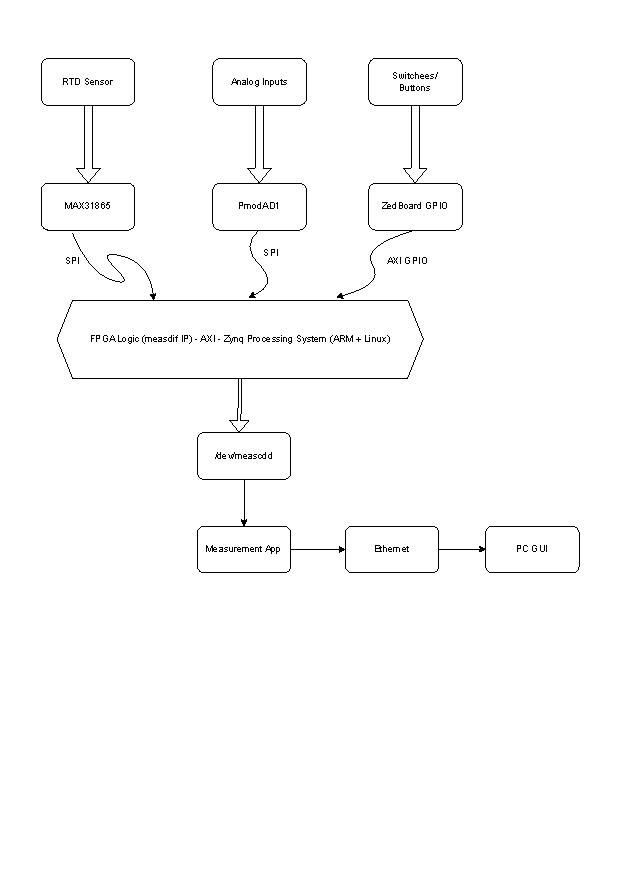
\includegraphics[width = 0.8\textwidth, trim = 0cm 4.5cm 0cm 0cm, clip]{media/hardArch.pdf}
\caption{Overall Hardware Architecrue of the Measurement Network Gateway}
\label{fig-reza1}
\end{figure}

\section{Zynq-7000 System-On-Chip Platform}
For the Measurement Network Gateway project the hardware implementation is based on only ZedBoard development platform that incorporates a Xilinx Zynq-7000 SoC. There are comprehensive set of  peripherals, including DDR3 memory, Ethernet connectivity, user input/output devices, and PMOD expansion connectors in this board. These features make the ZedBoard well suited for rapid prototyping of embedded measurement systems.

The ZedBoard acts as the central control unit of the system, hosting both the hardware interfaces implemented in programmable logic and the software environment running on the processing system. All external sensors and peripherals are physically connected to the ZedBoard, making it the focal point of the hardware design.

\begin{table}[H]
\centering 
\begin{tabularx}{\textwidth}{|X|X|X|}
\hline 
\textbf{Component} & \textbf{Purpose} & \textbf{Details} \\ \hline 
Dual ARM Cortex-A9 & Main Processor & Runs Linux kernel and application software \\ \hline 
FPGA Fabric & Custom Logic & Implements sensor interfaces, registers, timing logic \\ \hline  
DDR3 Memory & RAM & System memory for kernel and applications \\ \hline 
Ethernet MAC & Network Interface & Connects to lab network for TCP/IP communications \\ \hline 
GPIO Pins & Input / Output & User LEDs, switches, push buttons \\ \hline 
PMOD Headers & Expansions & Connectors for daughter boards (PmodAD1, MAX31865) \\ \hline 
\end{tabularx}
\caption{The Key Components on ZedBoard}
\end{table}

\begin{figure}[H]
\centering
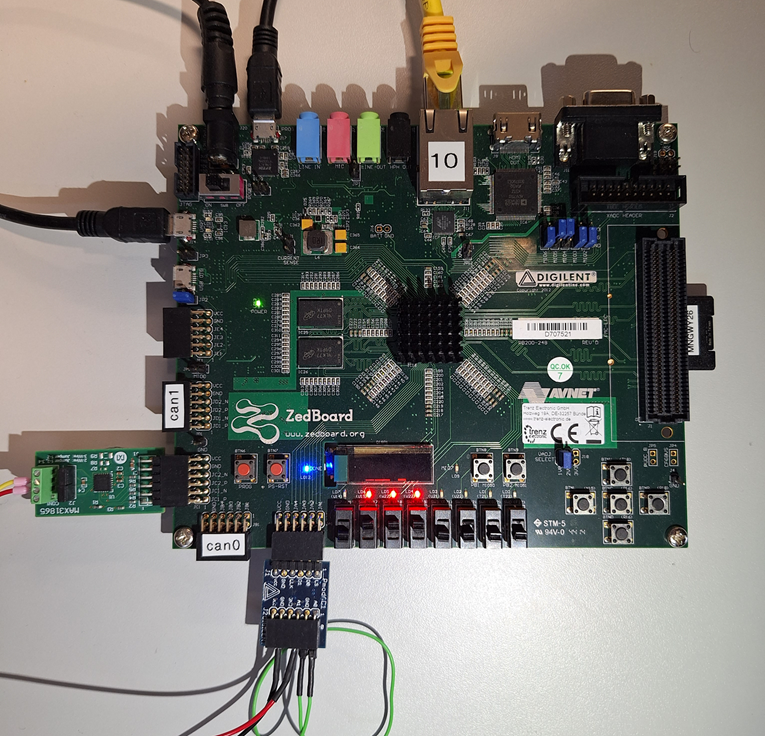
\includegraphics[width = \textwidth]{media/boardWithPeriph.png}
\caption{Zedboard development platform with connected peripherals}
\end{figure}

\subsection{Processing System}
In the processing system of Zynq-700, there is ARM Cortex-A9 processor running a Linux operating system generated using PetaLinux. This part of the system is responsible for the measurement application, managing network communication, and providing controlled access to hardware resources.

Linux is providing the stable runtime environment with a mature TCP/IP networking stack and a standardized device model. Hardware peripherals implemented in the programmable logic are exposed to user space through the /dev/meascdd character device and it allows the measurement application to contact with sensor for the read and write operations. With this approach, it is going to simplifies application development, improves portability, and separates hardware complexity from application logic.

So finally the process system is suited for those tasks that involves with complex protocols or variable execution timing which are such as TCP communication, command parsing, buffering, and interaction with a graphical user interface.

\subsection{Programming Logic (PL)}
In this part which is the programmable logic portion of the Zynq-7000 SoC, responsible for custom hardware interfaces for sensor communication and digital input/output. These interfaces are connected to the processing system via AXI interconnects, and they are enabling memory-mapped access to hardware registers.

For the measurement network gateway project the programmable logic implements SPI controllers for the PmodAD1 analog-to-digital converter and the MAX31865 RTD interface, as well as GPIO registers for switches, pushbuttons, and LEDs. The hardware is handling the Timing generation, conversion control, and status signaling. With the implementation of those functions in the FPGA fabric, the system achieves deterministic timing behavior and minimizes CPU load.

Programmable logic runs on its own clocks, independent of Linux, for precise sampling, parallel I/O, and dependable hardware interaction.
\begin{figure}[H]
	\centering 
	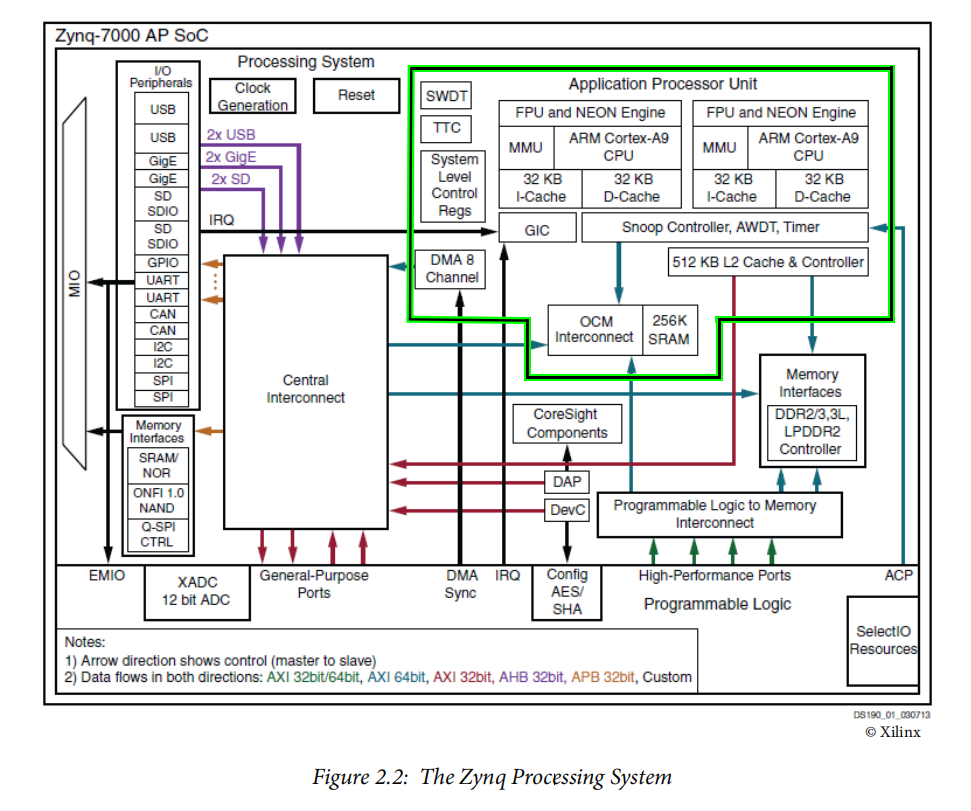
\includegraphics[width = 0.8\textwidth, trim = 0cm 1.5cm 0cm 0cm, clip]{media/processing.png}
	\caption{Zynq-7000 processing system architecture}
	\label{fig-zynq7000}
\end{figure}
	
\subsection{Division of Responsibilities between PS and PL}
The Zynq architecture distributes system functions between the Processing System (PS) and Programmable Logic (PL) based on timing requirements, implementation complexity, and suitability to hardware or software execution.

Time-Critical Functions in PL:
ADC signal acquisition and SPI communication are implemented in programmable logic because they require deterministic microsecond-scale timing. SPI bit clocks, chip-select windows, conversion start pulses, and sampling cadences must follow exact hardware timing constraints that are difficult to guarantee in software running under a preemptive operating system such as Linux. The FPGA fabric operates synchronously in well-defined clock domains, allowing sensor interfaces and GPIO sampling to execute independently of CPU load and operating system scheduling.

\subsubsection{High-Level Functions in PS}
In contrast, network communication and application logic are implemented in the processing system. TCP/IP protocol handling, socket management, command parsing, and ring buffer management involve complex, stateful operations that benefit from the mature Linux networking stack and device driver model. These functions tolerate millisecond-scale jitter without affecting measurement quality, making them well suited for execution in software on the ARM processor.

\subsubsection{Register Interface as the Bridge}
Memory-mapped registers serve as the clean boundary between hardware and software. PL logic based on its own clock domain is updating continuously sensor measurement registers, in this during the PS is reading and writing these registers via AXI interconnect and the /dev/meascdd device driver in the CPU clock domain. AXI and clock-crossing logic ensure safe data transfer, so software sees 32-bit measurements while the FPGA enforces real-time constraints.

\begin{figure}[H]
	\centering 
	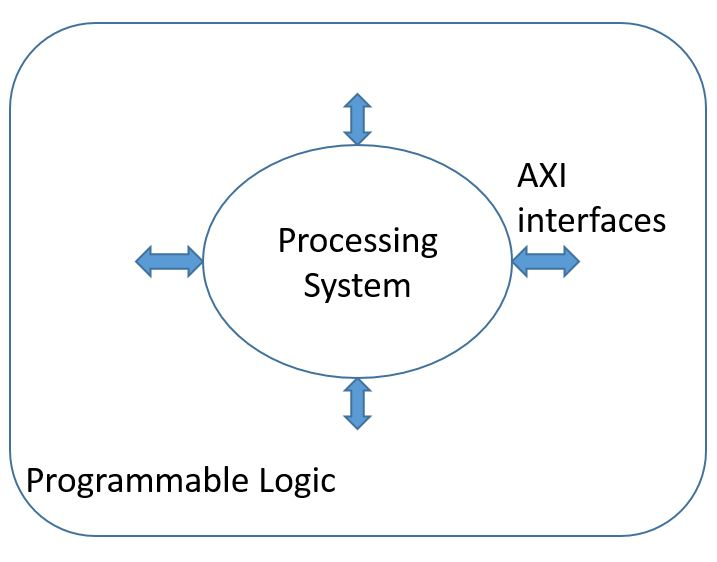
\includegraphics[width = 0.4\textwidth]{media/znyqArch.png}
	\caption{Zynq-7000 Processing System and Programming Logic Architecture}
	\label{fig-zynqProc}
\end{figure}

\section{Hardware Register Interace and Memory-Mapped I/O}
The interface between hardware and software in the Measurement Network Gateway is implemented using memory-mapped registers. This approach provides a well-defined, stable boundary that abstracts low-level hardware details from software while ensuring deterministic access to measurement data and control functions.

\subsubsection{Why we use Registers:}
Registers provide a small, well-defined set of 32-bit memory locations with stable read/write behavior. On the software point of view, each register, each register looks like a simple variable accessible through standard Linux drivers. The FPGA is handling all timing critical operations such as SPI sequencing, ADC conversion control, and GPIO handling. It isolates software from hardware details and allows hardware updates without altering applications.

\subsubsection{Register Structure}
Each register is implemented as a 32-bit word aligned on 32-bit boundaries, ensuring that AXI transactions from the Zynq PS map one-to-one to individual registers without unaligned accesses or partial writes. This simplifies both the Linux driver implementation (MeasObj\_struct with rnum and rvalue fields) and the PL logic that decodes address and data buses.
	
\subsubsection{Read/Write Semantics}
Register behavior is defined per address:

\begin{itemize}
	\item Read-only registers: Status flags, sensor data, GPIO input states
	\item Write-only registers: Control commands, LED outputs, conversion triggers
	\item Command/status registers: Writing initiates hardware action; subsequent reads return completion status or resulting data
\end{itemize}
This contract is captured in the measdif IP core specification and enforced by the /dev/meascdd device driver.

\subsubsection{Synchronization}
The PL updates registers in its own clock domain (typically derived from sensor or AXI clocks), while the PS reads or writes them in the CPU clock domain. The AXI interconnect and internal flip-flop staging ensure that each side sees only fully stable 32-bit values. This hardware-managed synchronization eliminates metastability and timing violations, making the register file the exact point where hardware meets software cleanly. The Linux driver never worries about SPI timing, ADC bit clocks, or clock-domain crossings—it simply reads and writes registers while the FPGA guarantees coherent, time-correct behavior underneath.

\subsection{Linux Device Driver}
The FPGA logic is exposed to the Linux kernel via a custom device driver:
\begin{itemize}
	\item Device file: /dev/meascdd (MEAScdd = Measurement Device)
	\item Type: Character device (read/write registers)
	\item Access method: ioctl() or direct read()/write() calls from C user-space
\end{itemize}
The driver provides memory-mapped register access:

\begin{minted}[bgcolor=lightgray, tabsize = 4, breaklines]{c}
	// Example: Read a status register
	int fd = open("/dev/meascdd", O_RDWR);
	uint32_t reg_value;
	read(fd, &reg_value, sizeof(uint32_t));
\end{minted}
	
\subsection{Hardware-Software Interface}
The boundary between hardware and software in the Measurement Network Gateway is implemented through a custom Linux character device, /dev/meascdd. This device provides a unified interface for accessing all measurement data and digital I/O states. Hardware registers in the programmable logic are mapped into kernel space and exposed to user-space applications through standard file operations.

With this approach, it shields applications from hardware details without losing performance or timing accuracy. Also it is going to simplifies the future modification to hardware, the changing is only effected with the driver part and will not touch or effect on user space software.

\begin{figure}[H]
	\centering 
	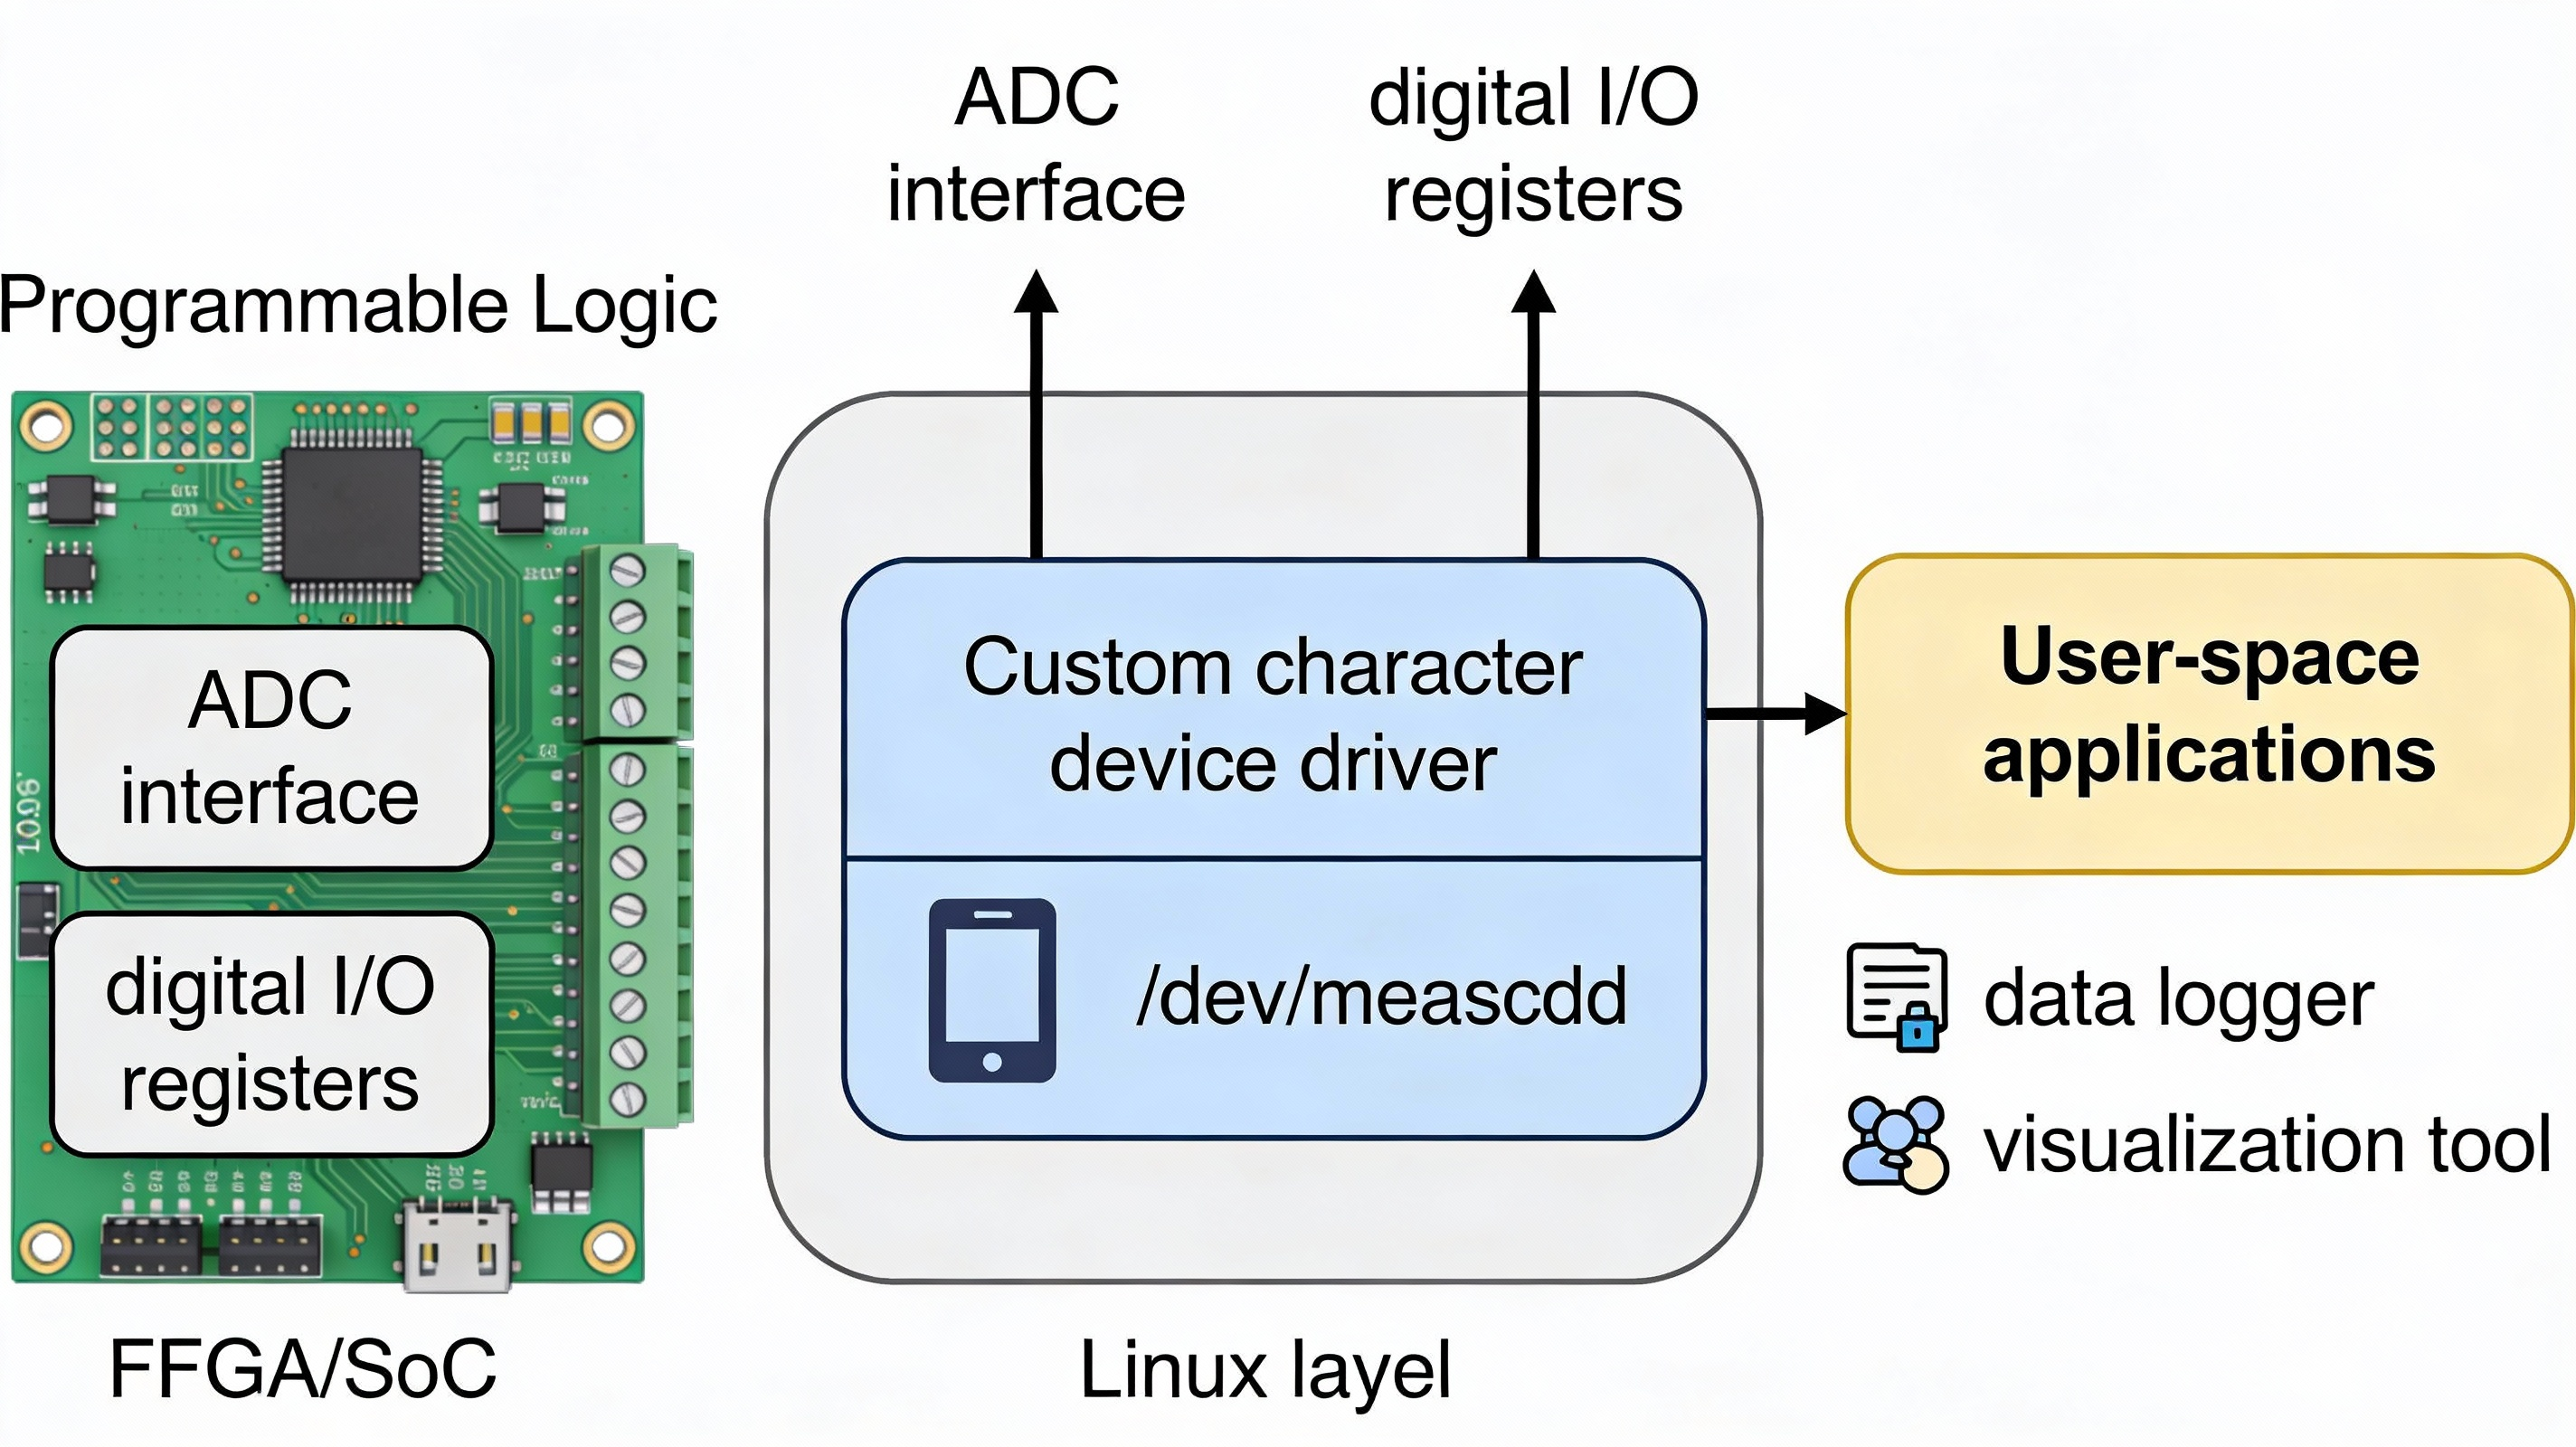
\includegraphics[width = 0.8\textwidth]{media/hard_soft.png}
	\caption{Hardware-Software interface through linux device driver}
	\label{fig-hard-soft}
\end{figure}

\section{Sensor Interface Subsystem}
The Measurement Network Gateway uses dedicated sensor interface subsystems to acquire physical signals and then convert them into reliable digital data, it will be needed for further processing. Each interface provides appropriate excitation, signal conditioning, and protection tailored to the specific sensor type, ensuring accurate and low-noise measurements even in industrial environments. 

\subsection{Temperature Measurement Subsystem}
Temperature measurement plays a key role in this system, because it is needed to monitor the condition of the equipment, apply temperature compensation to other sensors, and maintain safe operating limits in industrial use. For this reason, the gateway contains a dedicated temperature interface that delivers precise, stable temperature data for both laboratory experiments and real world deployments.

\subsubsection{RTD-Based Temperature Measurement}
Temperature measurement in the Measurement Network Gateway is implemented using a platinum Resistance Temperature Detector (RTD), specifically a PT100-type sensor. In the industry and laboratory is mostly used this RTDs because of their high accuracy, excellent long-term stability, and nearly linear resistance–temperature relationship over a wide operating range. If we compare to the semiconductor temperature sensor, it has different behavior. The RTDs provide predictable and repeatable behavior, making them suitable for precise measurements and calibration tasks.

The working principle of this RTDs is based on temperature-dependent resistance of platinum, with increasing of temperature the resistance of RTD element will increase in a good manner. With the correct measurement of the resistance and correctly conversion, the temperature will calculate and determined with high precision. In this project, the RTD serves as the primary sensing element, while all signal excitation, conditioning, and digitization are handled by a dedicated interface IC.

\begin{figure}[H]
	\centering 
	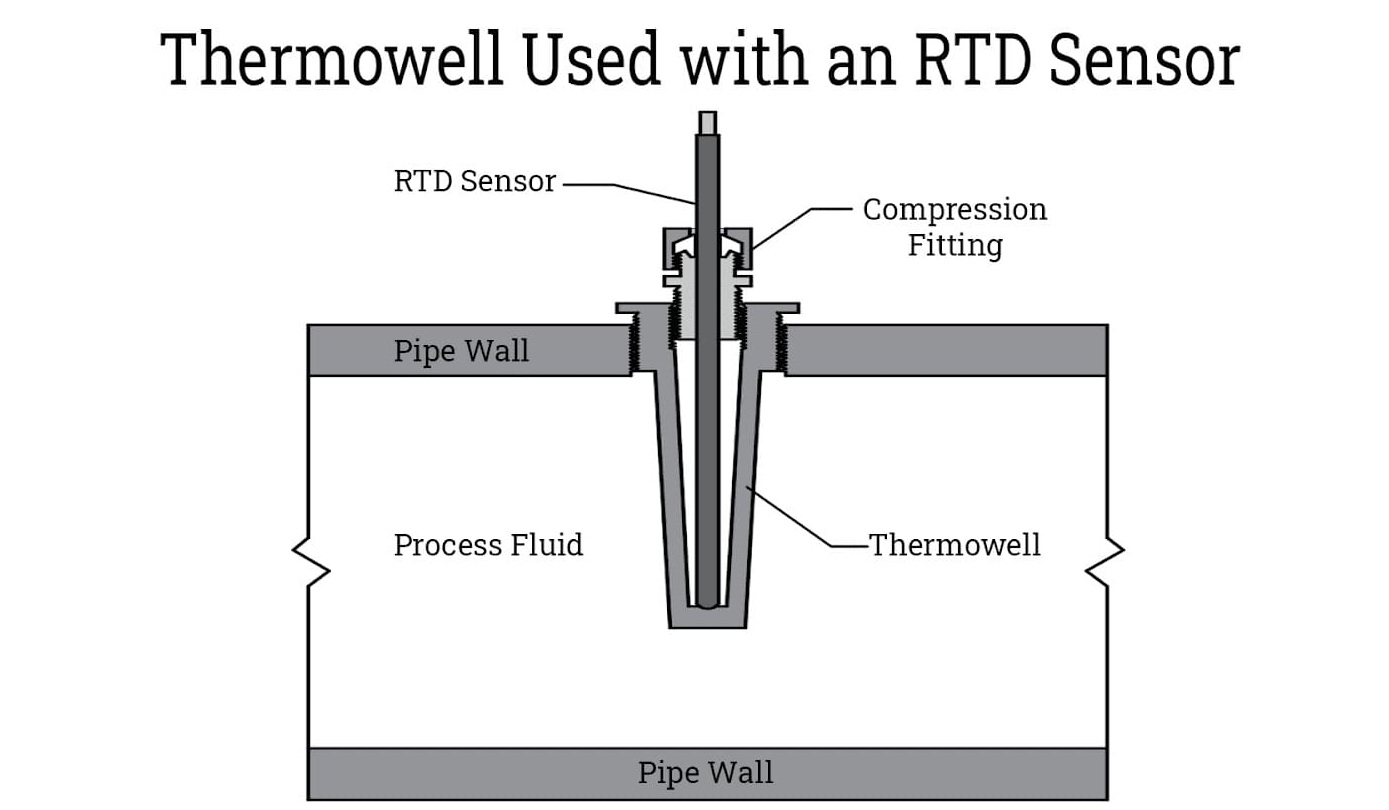
\includegraphics[width = 0.6\textwidth]{media/thrermal.jpg}
	\caption{Thermowell used with an RTD sensor}
	\label{fig-thermowell}
\end{figure}
	
\subsubsection{MAX31865 RTD-to-Digital Converter}
To interface the analog RTD sensor with the digital processing system, the design uses the MAX31865 RTD-to-digital converter. This integrated circuit is specifically designed for precision RTD measurements and significantly simplifies the hardware design. For the RTD, the MAX31865 provides a stable excitation current and measure the voltage drop and converting the resistance value into a digital representation using an internal high resolution analog to digital converter.

The MAX31865 supports multiple RTD wiring configurations, including 2-wire, 3-wire, and 4-wire setups. For our project the jumper setting allow the wiring mode to be selected based on the connected sensor on the module. This device has also the built in fault detection features such as open-circuit, short-circuit, and over-range detection, improving robustness and allowing hardware-level error identification.
The Serial Peripheral Interface (SPI) is a communication path between the MAX31865 and the Zynq platform. During system initialization, configuration registers inside the MAX31865 are programmed to set parameters such as wiring mode, fault detection options, and conversion settings and after the initialization periodic SPI transactions are executed to retrieve the latest conversion results. After initialization, periodic SPI transactions are executed to retrieve the latest conversion results. The achievable update rate is limited by the internal conversion time of the MAX31865 and is typically set to approximately 10 Hz in this project, which is sufficient given the slow dynamics of temperature changes.

Accuracy in this measurement chain is influenced by several factors, including the tolerance class of the RTD sensor, the reference resistor used by the MAX31865, ADC resolution, and PCB layout. Under typical laboratory conditions and with basic calibration, the system achieves temperature accuracy on the order of a few tenths of a degree Celsius to approximately ±1 °C. Environmental effects such as lead resistance and RTD self-heating are also relevant; long or thin wires increase series resistance, and excessive excitation current can slightly warm the sensor. These factors are mitigated through appropriate wiring configuration and conservative excitation settings.

\begin{figure}[H]
	\centering 
	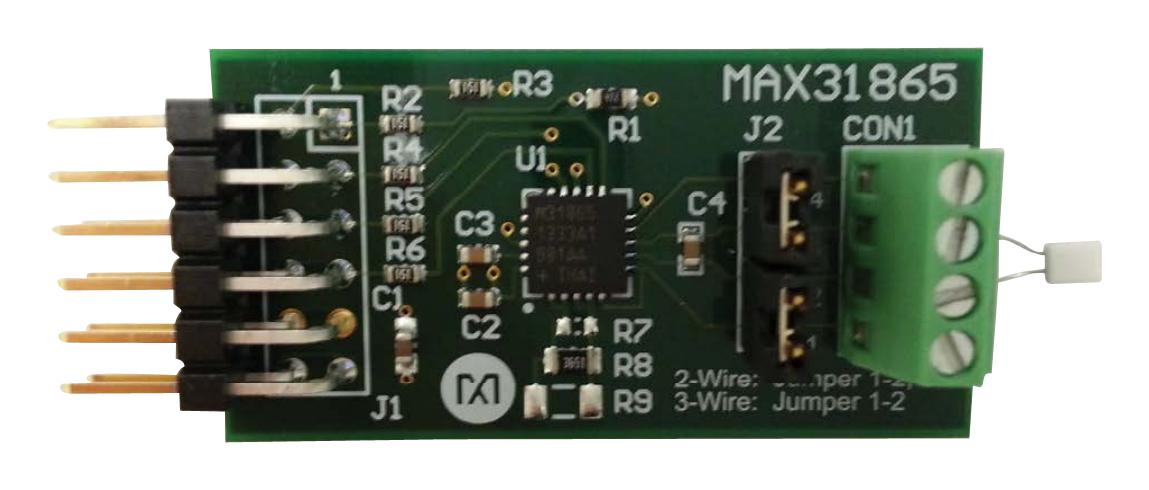
\includegraphics[width = 0.6\textwidth]{media/rtd.jpg}
	\caption{MAX31865 module with connected RTD sensor}
	\label{fig-rtd}
\end{figure}
	
	
\subsubsection{Integration into the Measurement System}
The temperature measurement subsystem is tightly integrated into the overall Measurement Network Gateway architecture through the programmable logic of the Zynq-7000 SoC. The FPGA-based programmable logic implements the SPI master that communicates with the MAX31865, ensuring precise timing and deterministic control of the SPI clock, chip select, and data signals. When a temperature conversion is complete, the programmable logic retrieves the digital result and stores it in memory-mapped registers connected to the AXI interconnect.

These registers are exposed to the processing system through the custom measdif hardware interface and accessed in software via the /dev/meascdd Linux character device. The user-space measurement application periodically reads the temperature registers, associates each value with a timestamp and a unique sensor identifier, and inserts the data into the shared ring buffer. From there, the measurements are forwarded to the network subsystem and transmitted to the remote graphical user interface.

This hardware–software partitioning ensures that all time-critical tasks, including SPI timing, conversion control, and data latching, are handled deterministically in hardware, while higher-level tasks such as buffering, networking, and visualization are managed in software. The result is a robust, accurate, and industry-relevant temperature measurement solution that integrates cleanly into the overall gateway architecture.

\begin{table}[H]
	\centering 
	\begin{tabularx}{\textwidth}{|X|X|}
		\hline 
		\textbf{Parameter} & \textbf{Value} \\ \hline 
		RTD Type & PT100 \\ 
		Update Rate & $\approx \SI{10}{\hertz}$ \\ 
		Typical Accuracy & $\pm\ 0.5$ to $\pm \SI{1.0}{\degreeCelsius}$ (Uncalibrated) \\ 
		Interface & SPI via MAX3865 \\ \hline 
	\end{tabularx}
	\caption{Key Specification of the RTD-Based temperature Measuremnt}
\end{table}

\subsection{Analog Data Acquisition Subsystem}
The analog data acquisition subsystem converts the low-level analog signals into the precise digital values which is processed by the FPGA and embedded software. It is going to provide the required input range, resolution, and sampling performance to capture slow- and medium-speed sensor signals without distortion, when it ensures stable and repeatable measurements through proper interfacing and timing control.

\subsubsection{PmodAD1 Analog-to-Digital Converter}
The PmodeAD1 module which is responsible for the measurement of  analog voltage in this project and PmodAD1 integrates two Analog Devices AD7476A 12-bit successive-approximation ADCs which provide two independent single-ended analog input channels. Each converter operates over a voltage range of approximately 0 V to 3.3 V, referenced to the ZedBoard’s analog supply.

The chip select and serial clock which are the control signal, and also the data transfer on the MISO line are generated and handled by the programmable logic. This hardware-driven SPI implementation ensures deterministic sampling behavior and avoids timing jitter associated with software-controlled I/O.

Mechanically and electrically, the PmodAD1 is connected to the ZedBoard through the JA1 Pmod header. The 2×6 pin Pmod connector directly maps FPGA I/O pins to the ADC control and data signals, allowing low-latency and tightly synchronized communication between the ADC and the FPGA fabric.

\begin{figure}[H]
	\centering 
	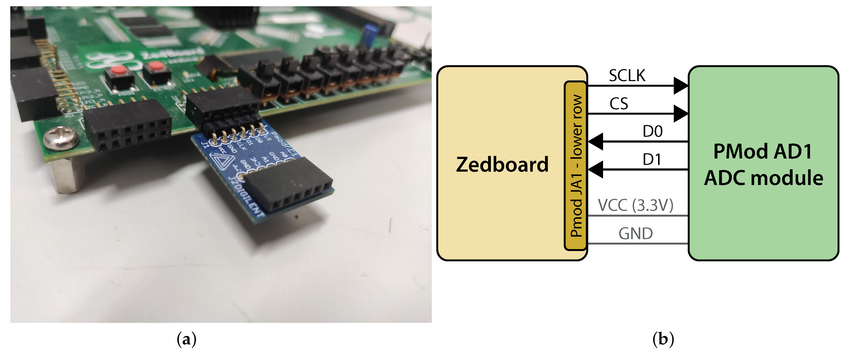
\includegraphics[width = 0.6\textwidth]{media/pmod.png}
	\caption{PmodAD1 module mounted on the Zedboard}
	\label{fig-pmod}
\end{figure}

\textbf{Specification:}
\begin{table}[h]
	\centering
	\caption{ADC Specifications}
	\begin{tabular}{ll}
		\toprule
		\textbf{Parameter} & \textbf{Value} \\
		\midrule
		Resolution & 12 bits \\
		Number of Channels & 2 (A0, A1) \\
		Input Range & 0 to 3.3\,V (configurable) \\
		Sampling Rate & Programmable via software \\
		Interface & SPI (MOSI, MISO, CLK, CS) \\
		Supply Voltage & 3.3\,V (from ZedBoard) \\
		\bottomrule
	\end{tabular}
	\caption{PmodAD1 Analog-to-Digital Converter Specification}
\end{table}

\subsubsection{Signal Acquisition and Conversion Characteristics}
External analog signals are supplied using laboratory equipment such as a function generator. And these all signals are applied through the PmodAD1 analog input channels. While the operation, the programmable logic is going to initiates SPI transaction at the chosen sampling rate, starts ADC conversions, and reads the digital values.

Each AD7476A produces a 12-bit value between 0 and 4095 for the full-scale input range. With a 0–3.3 V range, each LSB represents roughly 0.8 mV. The ideal quantization error is therefore ±0.5 LSB, although practical measurements also include additional uncertainty due to ADC offset, gain error, reference voltage stability, and noise.

The ADC reference voltage is derived from the ZedBoard’s regulated 3.3 V rail. As a result, any ripple or drift on this supply directly affects conversion accuracy. The clock derived from the FPGA fabric is responsible for sampling timing and the stability of this clock ensures consistent sampling intervals and minimizes timing jitter, which is particularly important when observing dynamic signals such as sine waves.

\begin{figure}[H]
	\centering 
	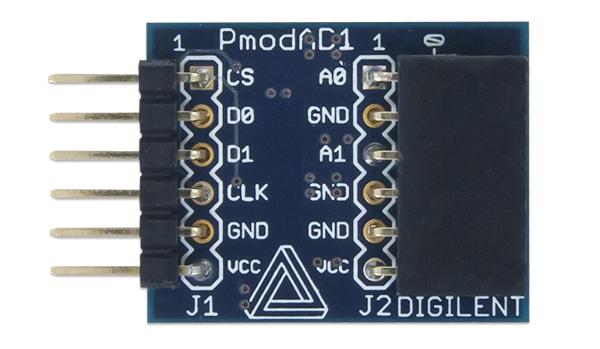
\includegraphics[width = 0.3\textwidth]{media/pmod2.png}
	\caption{Analog data acquisition using PmodAD1}
	\label{fig-pmod2}
\end{figure}

\subsection{Digital Input and Output Interfaces}
The digital input and output interfaces of the Measurement Network Gateway is going to provide the main means for user interaction and simple control signaling. They connect board-level switches, pushbuttons, and GPIO signals to the programmable logic, it is enabling the manual test inputs, status indication, and coordination with external devices.  With the exposing of these signals through memory-mapped registers and Linux drivers, the system allows software to monitor and control digital I/O flexibly and reliably.


\subsubsection{Switches and PushButtons}
The ZedBoard includes user-accessible switches and pushbuttons connected to the programmable logic through GPIO interfaces. These inputs operate at 3.3 V logic levels and are buffered by on-board circuits that include fixed pull-up or pull-down resistors to ensure defined logic states when switches are open. Logic '1' and '0' correspond to 3.3 V and 0 V at the FPGA input pins, as defined by the ZedBoard schematic and FPGA pin constraints.

Debouncing is handled primarily in software. The sensor layer samples GPIO states at a moderate rate (typically tens of Hz), and brief contact bounce is either filtered by this sampling interval or can be ignored for the measurement use case. No additional RC networks or Schmitt-trigger circuits were required, as the ZedBoard's user I/O already provides adequate buffering and signal conditioning.
The digital state of all switches and pushbuttons is read by the FPGA and stored in memory-mapped GPIO input registers. The Linux device driver exposes these values to user-space software, allowing the measurement application to monitor user interactions and use them for testing, debugging, or basic control functions.

\subsubsection{LEDs}
User LEDs on the ZedBoard are controlled through GPIO output registers implemented in the programmable logic. Each LED is driven from an FPGA output pin through an on-board series current-limiting resistor that restricts current to a few milliamps. This current level is safe for the FPGA I/O and provides sufficient brightness for clear visual indication.

The measurement application uses the LEDs to provide real-time visual feedback. For example, LED states can mirror the current position of input switches, indicate active sampling, or signal connection status. Because the current-limiting resistors are already present on the board, the software can safely write switch bits directly to LED outputs without risk of over-current.

\begin{figure}[H]
	\centering 
	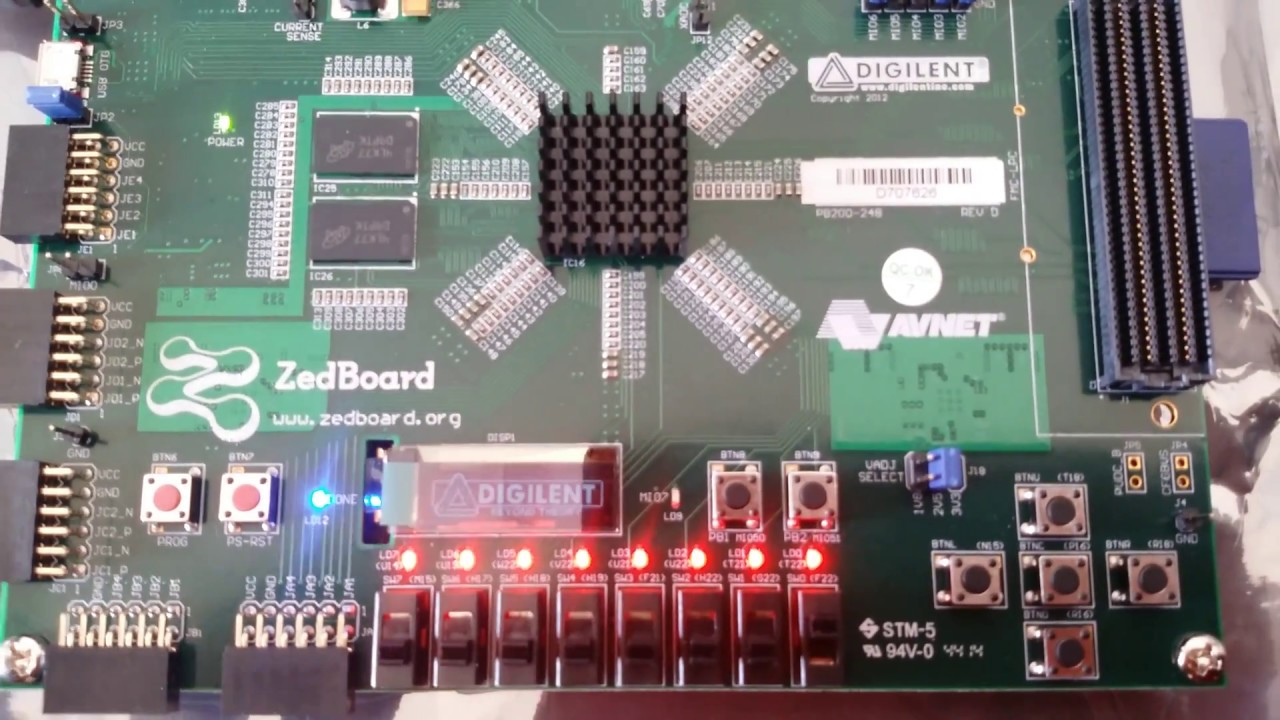
\includegraphics[width = 0.6\textwidth]{media/leds.jpg}
	\caption{ZedBoard user interface showing switches and LEDs in operation}
	\label{fig-leds}
\end{figure}

\subsubsection{Ethernet and Network Interface}
The Measurement Network Gateway uses the integrated Ethernet interface of the Zynq processing system to communicate with external clients. The external PHY connection which the Ethernet controller connected to that, it is providing a standard RJ45 interface. It allows the system directly connect to a local network or a single host computer for that hardware configuration

The Ethernet interface enables the transmission of measurement data using TCP/IP, providing reliable and ordered data delivery. The use of standard networking protocols ensures compatibility with a wide range of client systems.
\begin{figure}[H]
	\centering 
	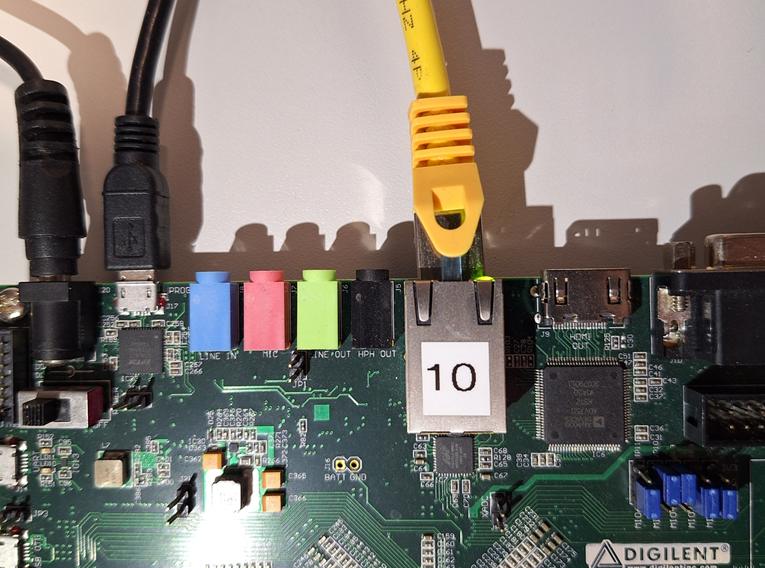
\includegraphics[width = 0.6\textwidth]{media/ethernet.png}
	\caption{Ethernet Connection between the Zedboard and host PC}
	\label{fig-ehternet}
\end{figure}

\section{Timing, Interrupts and Hardware synchronization}
Reliable and deterministic timing is a fundamental requirement of the Measurement Network Gateway, as multiple sensors must be sampled at well-defined intervals while operating within a Linux-based environment. To avoid the nondeterministic behavior associated with software-based delays, all timing-critical operations are implemented in hardware inside the programmable logic (PL) of the Zynq device. Interrupts and status signaling mechanisms are then used to synchronize these hardware events with the processing system (PS).

\subsection{Hardware Timing Sources}
Timing events in the system are generated by clocked hardware implemented in the programmable logic. A base fabric clock (for example 100 MHz) is divided down using counters and clock-enable logic to create slower, application-specific timing signals. These timing signals set the controlling ADC sampling intervals, MAX31865 temperature conversion cycles, and GPIO sampling rates.

Each hardware timing logic is responsible for the its own sensor interface and it ensures the sampling occurs at precise and repeatable intervals independent of the Linux scheduler. This approach guarantees deterministic sampling behavior and allows multiple sensors to operate concurrently at different configured frequencies.

\subsection{Interrupt and Event Handling}
When a sensor conversion or measurement cycle completes, the programmable logic sets dedicated status bits in memory-mapped registers exposed through the measurement interface. Examples include “ADC done” or “MAX31865 conversion complete” flags. The processing system monitors these events either by polling the status registers or, in a more advanced configuration, through hardware interrupts.

Interrupts allow the ARM processor to remain idle or perform other tasks instead of continuously polling registers. When an interrupt is asserted from the PL to the PS, the Zynq Generic Interrupt Controller (GIC) wakes the processor, which then reads the corresponding data and status registers, stores the sample into the ring buffer, and resumes normal operation. This mechanism improves CPU efficiency while maintaining fast response times.

\subsection{Synchronization Strategy}
Synchronization between sensor sampling and software processing is achieved through a combination of hardware-controlled timing and software-level timestamping. Because the sampling instants are defined by hardware clocks in the PL, the timing of each measurement is stable and predictable. When the processing system retrieves a sample, it associates it with an elapsed-time or timestamp value to preserve temporal ordering.

If interrupts are missed due to masking, overload, or software faults, the hardware continues sampling at the correct rate, but samples may remain unread in registers or be overwritten by newer data. This can result in dropped measurements or stale data. To mitigate this risk, the software includes timeout checks and buffer management mechanisms to detect abnormal conditions and apply corrective actions, such as reporting errors or reducing sampling frequency.

\section{Measurement and Validation Equipment}
Validation of the Measurement Network Gateway hardware is performed using standard laboratory measurement equipment to observe signals at different points along the measurement chain. The objective of this validation is to confirm correct electrical behavior, timing integrity, and correspondence between physical signals and digital measurement results produced by the system.

The validation process focuses on three main areas: analog signal integrity at the sensor inputs, correct operation of digital communication interfaces such as SPI, and consistency between measured values and trusted reference instruments.

\begin{figure}[H]
	\centering 
	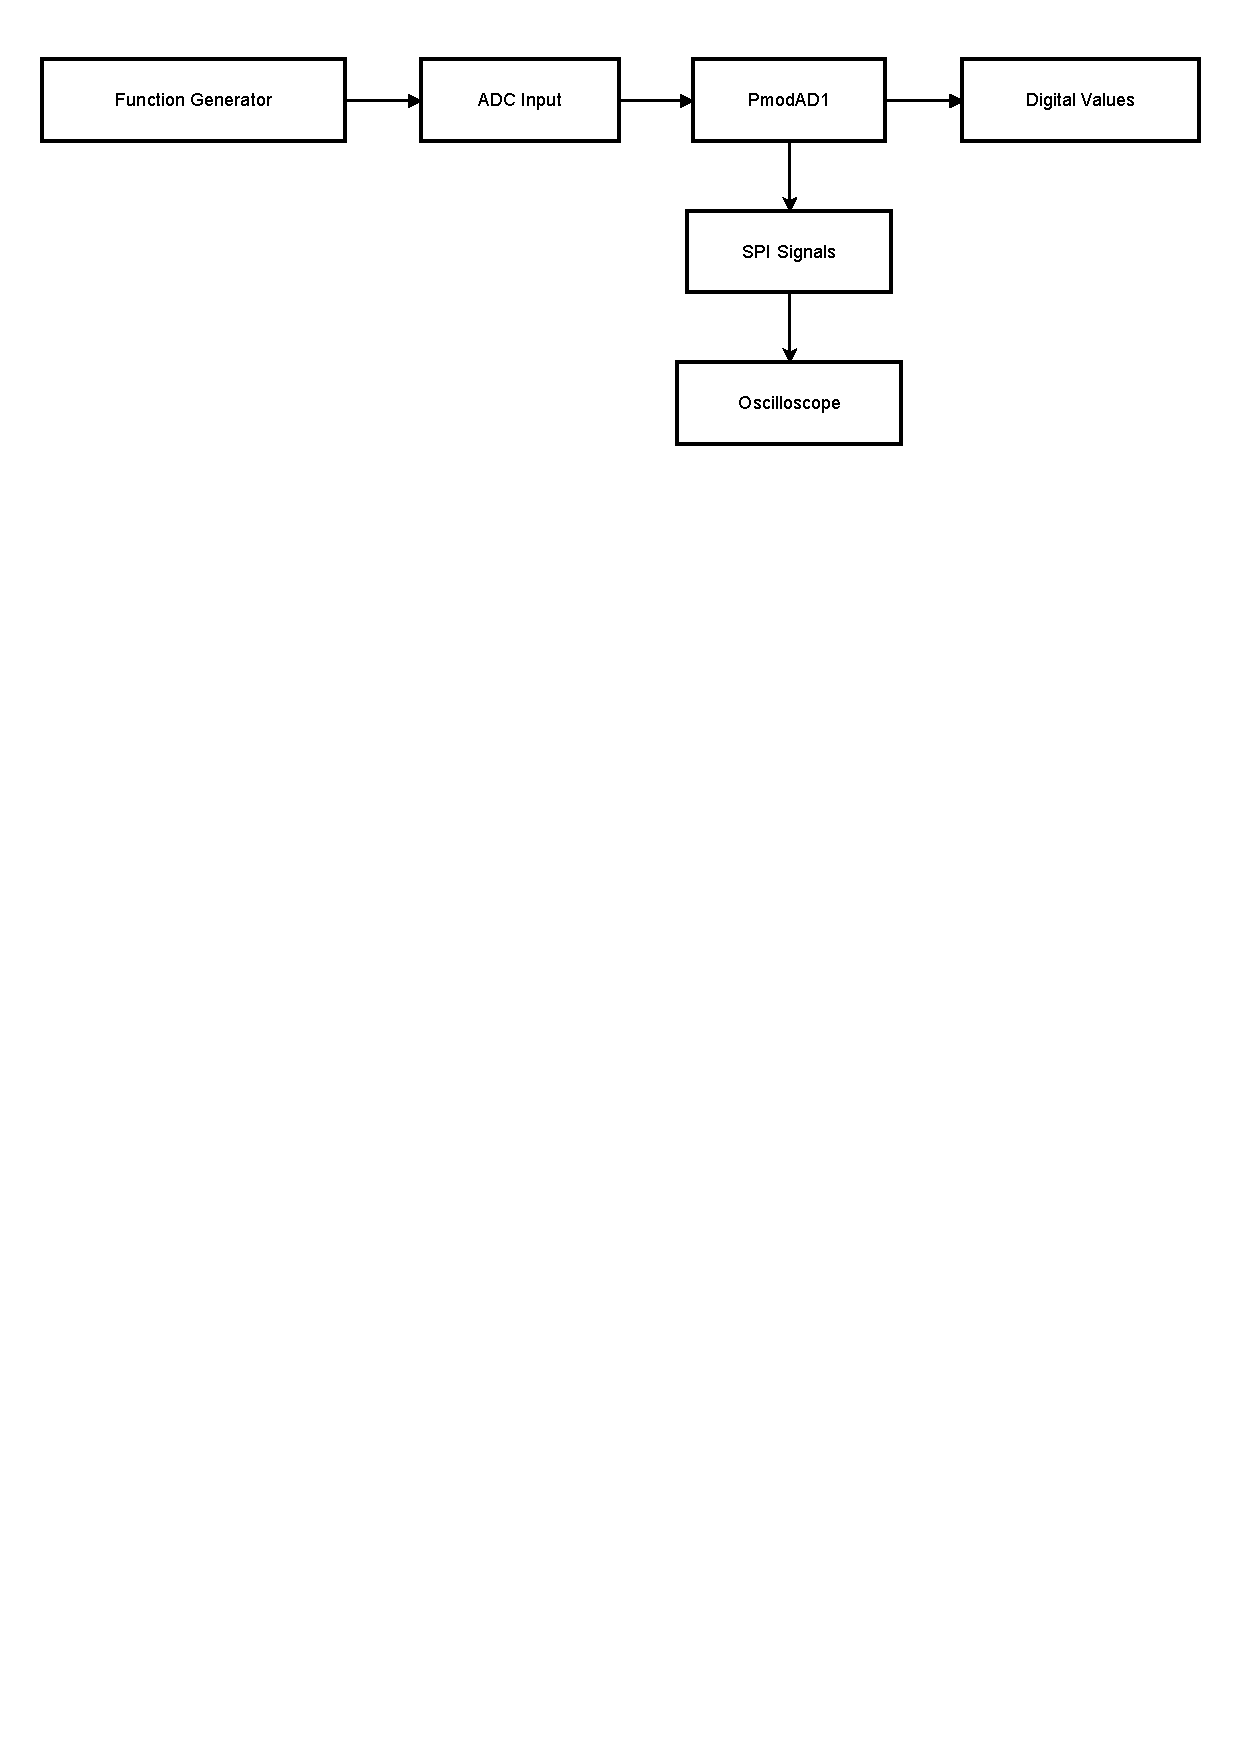
\includegraphics[width = 0.9\textwidth, trim = 0cm 22cm 0cm 0cm, clip]{media/validation.pdf}
	\caption{Validation Measurement Point}
	\label{fig-validation}
\end{figure}

\subsection{Validation Methodology}
During validation, external instruments are used to generate known input signals and to observe internal hardware signals. For the ADC subsystem, a function generator provides controlled DC or sinusoidal voltages to the PmodAD1 inputs. These signals are monitored directly using an oscilloscope and multimeter, while the corresponding digital output values are read from the gateway.

SPI communication between the Zynq programmable logic and peripheral devices such as the PmodAD1 ADC and MAX31865 temperature sensor is examined by probing the clock, chip-select, and data lines. Correct operation is indicated by stable clock frequency, clean chip-select timing, and consistent data transitions synchronized with the clock edges.

Fault conditions can be identified by characteristic symptoms, including distorted or clipped analog waveforms, missing or irregular SPI clock pulses, static data lines despite changing inputs, excessive noise or jitter in ADC codes, or systematic offset and gain errors compared with reference measurements.

\subsection{Laboratory setup and Reference Equipment}
The validation setup uses standard laboratory instruments to provide controlled inputs, stable power, and accurate reference measurements. These instruments allow both static and dynamic verification of the measurement chain and ensure repeatable test conditions.

Key equipment includes:
\begin{itemize}
	\item Function generator for analog input signals
	\item Regulated laboratory power supplies
	\item Digital multimeter for reference voltage and current measurements
	\item Digital storage oscilloscope for timing and signal integrity analysis
\end{itemize}

\subsection{Hameg Triple Power Supply and Digital Multimeter}
It is one of the power supply which is used for the stable and low noise DC power to the ZedBoard, sensor modules, and auxiliary circuits. It has multiple independent and different outputs which allow different subsystems to be to be powered and tested under controlled conditions, while adjustable voltage levels and current limiting protect the hardware during experimentation. 

For the reference instrument of static electrical measurement used the HM8011-3 digital multimeter which provide high resolution readings of voltage and current, enabling precise monitoring of supply rails, sensor excitation voltages, and calibration points. By comparing these reference measurements with the digital values reported by the gateway’s ADC subsystem, offset errors, gain errors, and overall measurement accuracy can be evaluated.
\begin{figure}[H]
	\centering 
	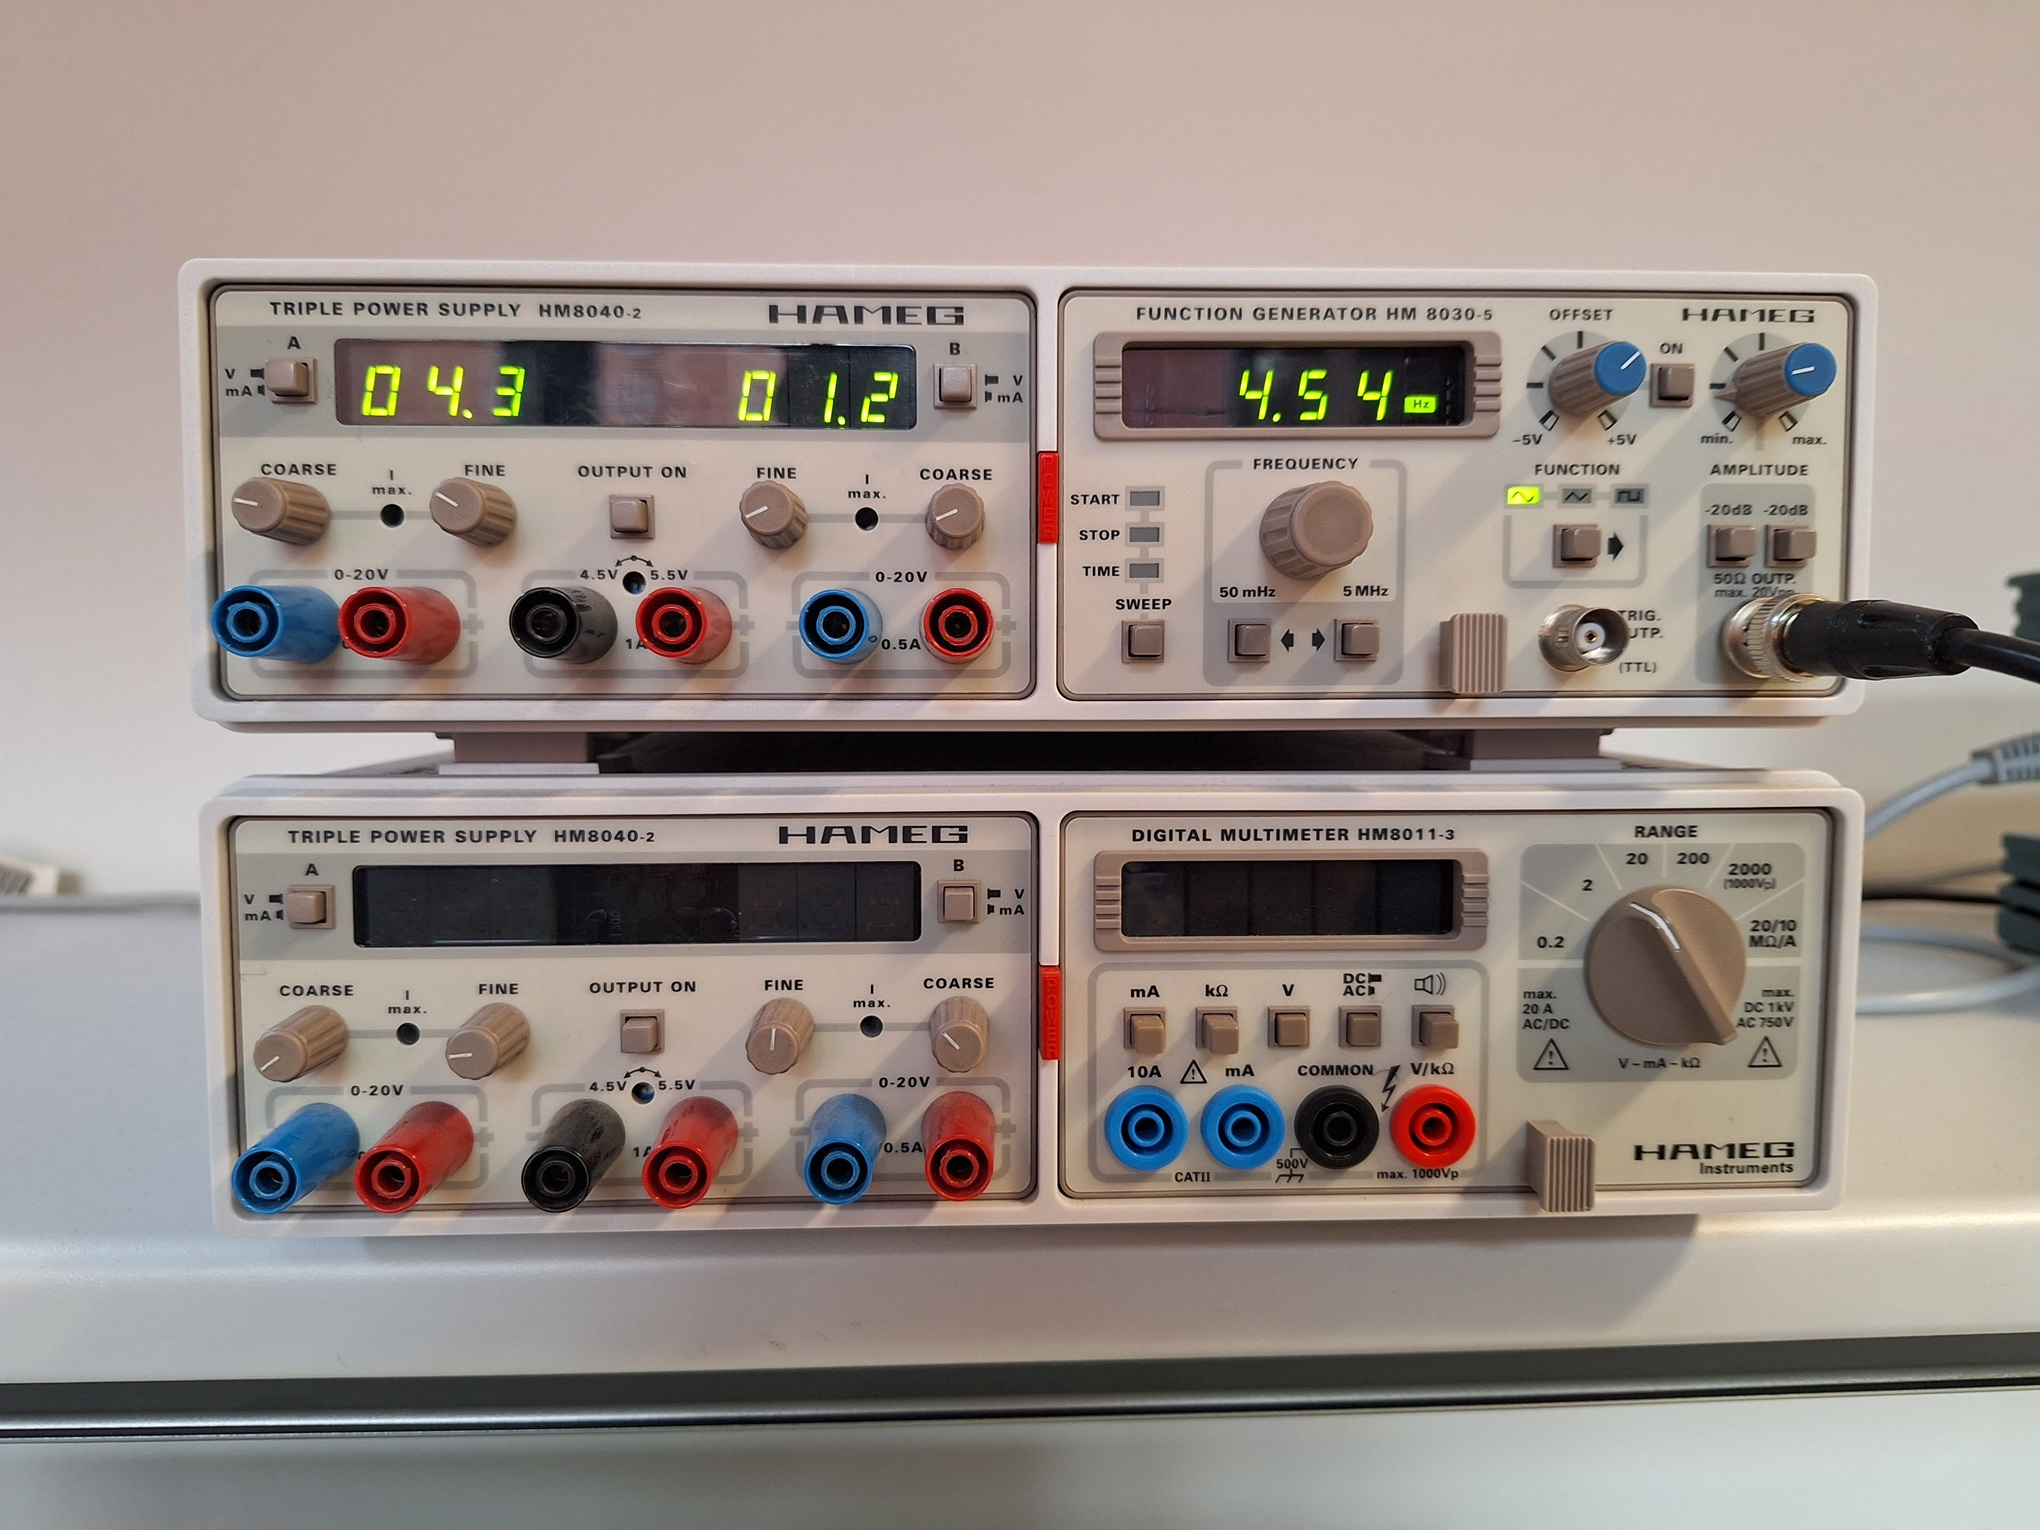
\includegraphics[width = \textwidth]{media/ocsi.jpg}
	\caption{Hameg power supply and multimeter used for power delivery and reference measurements}
	\label{fig-ocsi}
\end{figure}

\subsection{Tektronix TDS2014B Digital Storage Oscilloscope}
The Tektronix TDS2014B digital storage oscilloscope is used to analyze the dynamic behavior of both analog and digital signals within the system. Its four-channel input, 100 MHz bandwidth, and real-time sampling capability of up to 1 GS/s allow simultaneous observation of multiple signals.

Typical measurements include the analog input waveform applied to the ADC, the SPI clock and chip-select signals, and the serial data lines. Time-domain analysis is used to verify waveform shape, amplitude, and timing relationships, while triggering and automated measurements assist in checking setup and hold times and identifying potential timing violations.

The oscilloscope’s FFT capability is also used to assess noise and harmonic content in analog signals. This makes it possible to correlate observed noise or distortion in the digital measurement results with physical effects on the analog input or communication lines.

\begin{figure}[H]
	\centering 
	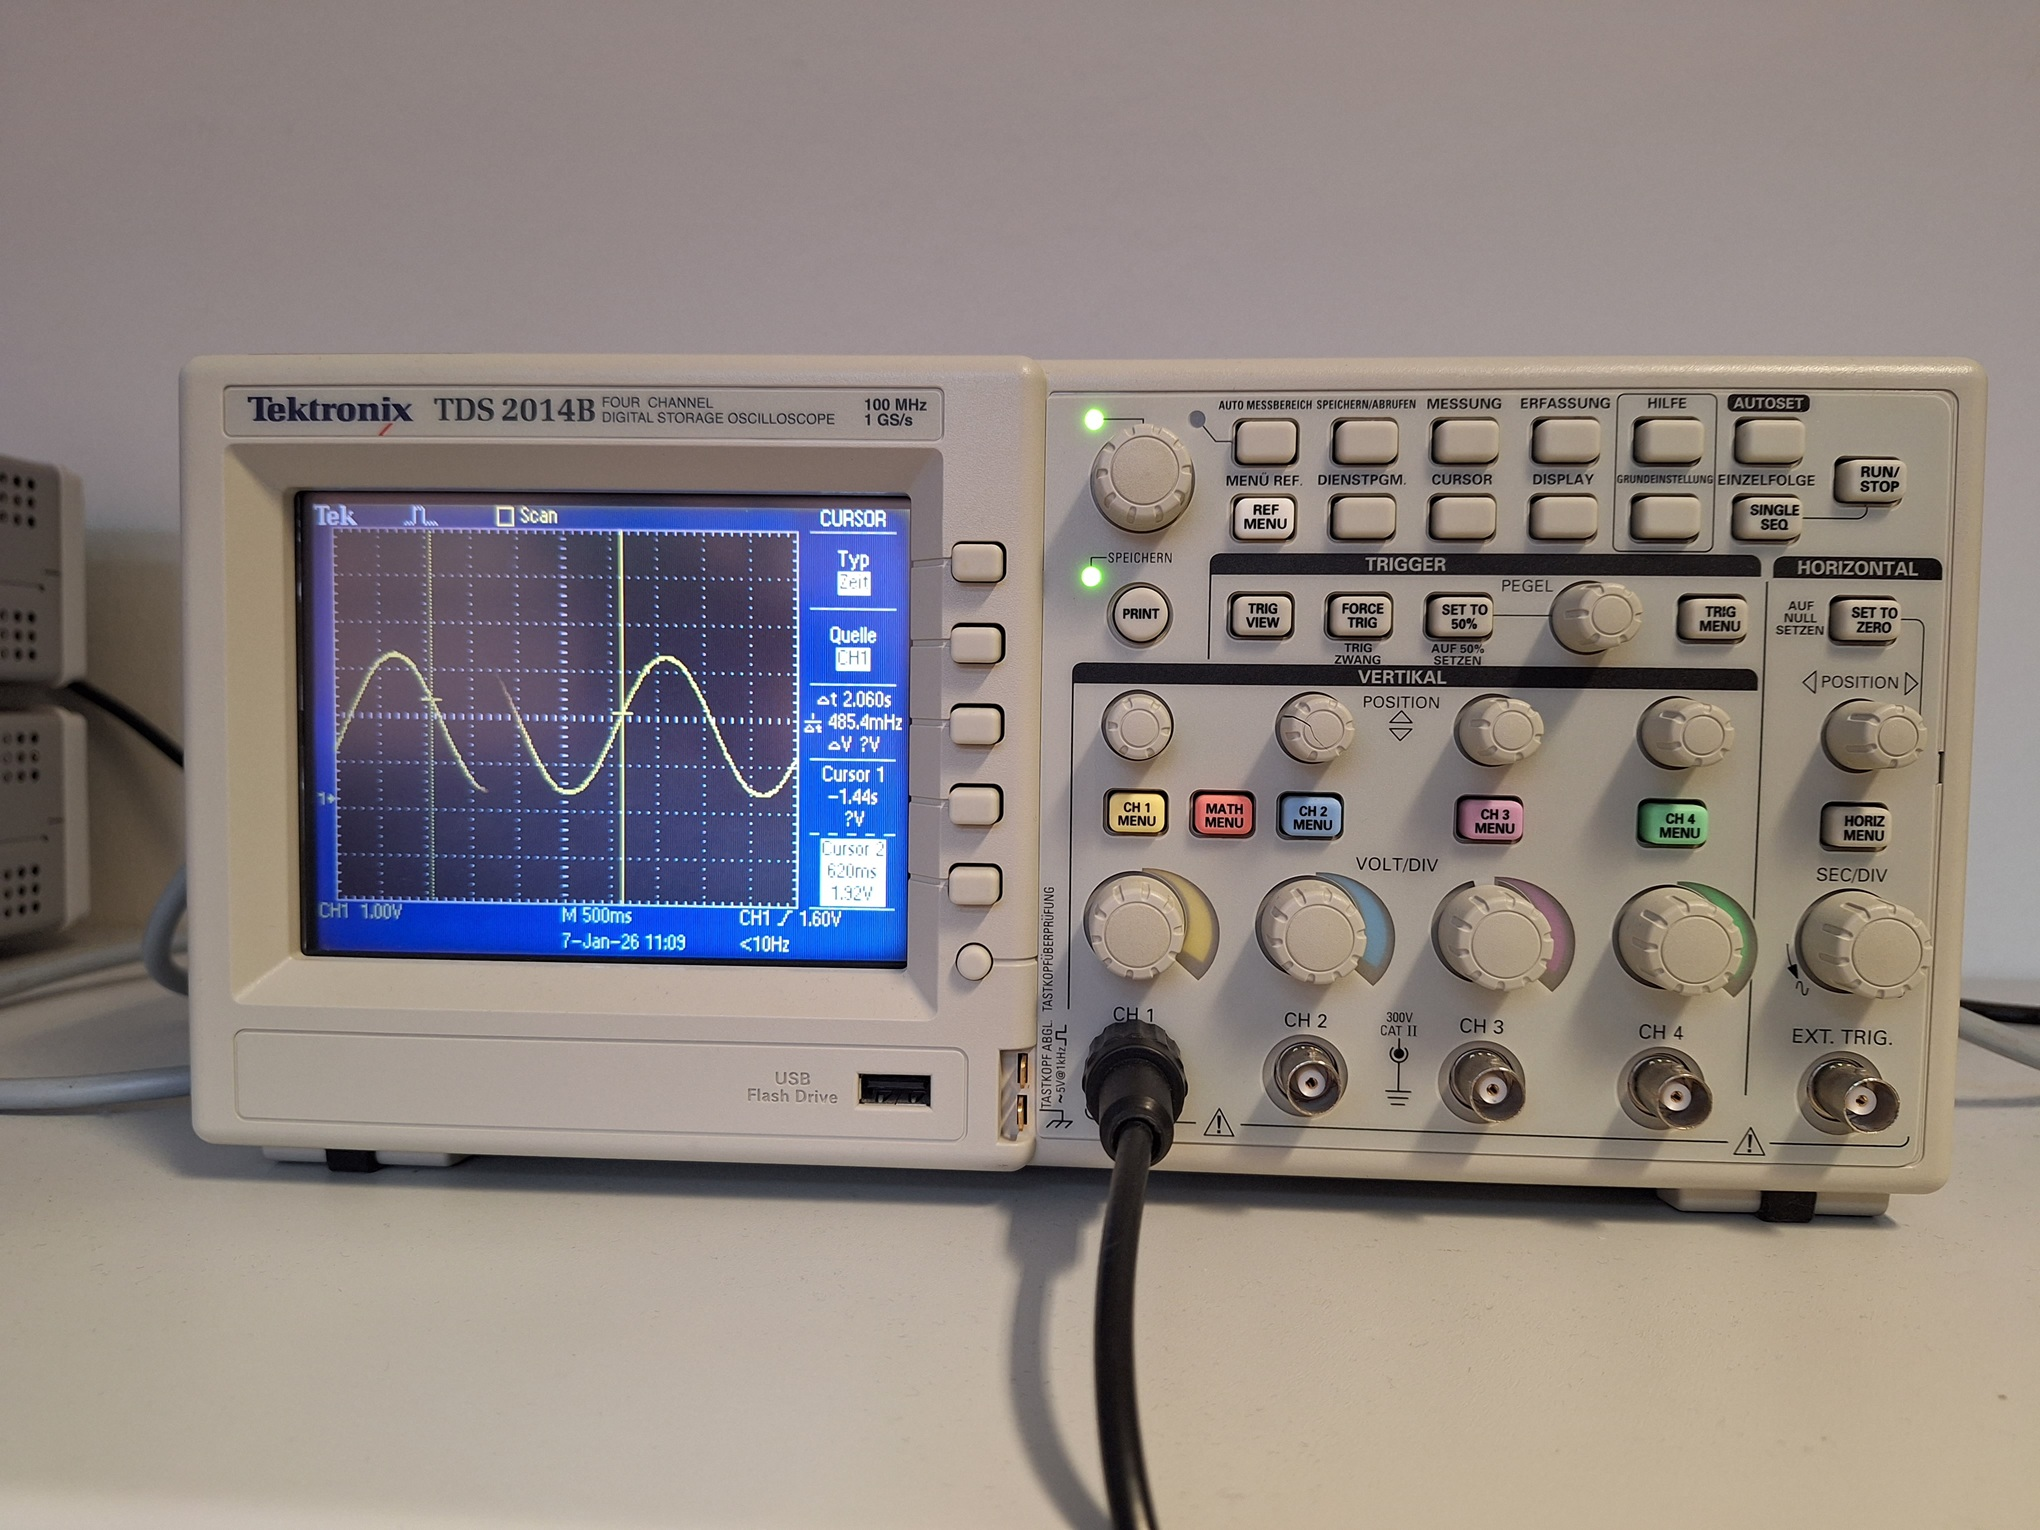
\includegraphics[width = \textwidth]{media/func.jpg}
	\caption{Oscilloscope measurement of SPI timing during ADC conversion.}
	\label{fig-func}
\end{figure}

\subsection{Discussion and Design Considerations}
The measurement and validation results confirm that the hardware design meets its intended functional requirements under laboratory conditions. The FPGA based timing control with combination of Linux based processing will provide reliable operation while keeping hardware complexity manageable.

The Validation of system is being simplifies with the modular structure which can act as individual subsystem for testing independently before being integrated. While the current setup is suitable for educational and general-purpose laboratory measurements, the validation process also highlights areas where additional filtering, shielding, or isolation would be required for high-precision or industrial applications.

\section{Hardware Safety, Reliability, and Robustness}
The hardware platform of the Measurement Network Gateway is designed with fundamental safety and robustness features which is suitable for laboratory and educational environments. It relies on low-voltage signal levels, which is integrated protection features of the ZedBoard, and also deterministic FPGA-based control to reduce the risk of damage, unsafe conditions, or unexpected behavior during normal operation. Together, these measures provide an appropriate level of electrical safety and reliability for the intended environment, which is allowing additional external protections to be added for harsher industrial deployments.

\subsection{Electrical Safety}
The hardware design operates entirely within low-voltage domains suitable for laboratory and educational use. All sensor interfaces, including the PmodAD1 ADC inputs and the MAX31865 RTD interface, operate at 3.3 V logic levels, which are safely supported by the ZedBoard and its FPGA I/O banks. RTD sensor wiring carries only low-level excitation currents and voltages, ensuring no exposure to hazardous energy levels.

The electrical protection is going to provide by Zed Board ’s on board input buffers, series resistors, and ESD protection. This design is not providing  galvanic isolation, surge suppression, or overvoltage protection suitable for industrial environments, for such kind of protections would need to be added externally using isolation amplifiers, TVS diodes, or opto-isolators if the system were deployed in the field. 

\subsection{Reliability Considerations}
The reliability of system is determined by  clock stability, power integrity, and deterministic hardware behavior. The ZedBoard provides a stable power rails for the processing system and programmable logic, and it also minimize the risk of brownouts during normal laboratory operation. All analog and digital modules share a stable 3.3 V supply, which is essential for ADC accuracy and temperature measurement precision.

FPGA logic guarantees predictable timing for critical functions. Unlike software-driven I/O, the programmable logic executes state machines and counters with predictable latency, independent of CPU load or operating system activity. This determinism is a key factor in achieving reliable, repeatable measurements.

\subsection{Fault Handling and Robustness}
This system is designed to control  and handle the general fault condition carefully. On the startup Zynq boot process resets both the PS and PL simultaneously, loads the FPGA bitstream, and initializes all custom registers to a known safe state. After Linux has fully booted then the sensor will start the conversions and the user-space application opens the /dev/meascdd device.

If the required conditions are failed such as unstable power, missing device files or unavailable hardware. The software avoids uncontrolled hardware access and either reports an error or switches to a fake-data mode for testing. When the communication is lost with the GUI, it can be handle by closing the client socket and waiting for testing, while invalid or missing sensor data is detected through timeouts and buffer checks.

\section{Design Limitations and Trade-offs}
The prototype prioritizes correctness and flexibility rather than performance or channel count. This design introduces practical limitations due to hardware, FPGA resource, and communication constraints. This section is going to summarize the main constraints on sampling rate and logic utilization and explains how these trade-offs influence the types of applications the system is best suited for.

\subsection{Sampling Rate Limitations}
The maximum achievable sampling rate is limited by several factors, including SPI bus bandwidth, ADC conversion time, PL state machine latency, and the rate at which the PS can read registers and store data in the ring buffer. As a result, each sensor channel operates reliably at hundreds of samples per second rather than at high-speed MHz-level rates.

This limitation is acceptable for slowly varying signals such as temperature, voltage monitoring, and digital inputs but makes the system unsuitable for high-speed data acquisition applications without significant hardware changes.

\subsection{Hardware Resource Constraints}
The programmable logic is going to implement only a fraction of the Zynq FPGA resources are used for SPI, counters, GPIO, and AXI. There is room to expand, but LUTs, flip-flops, and block RAM are still finite.
Adding many more sensors, parallel ADCs, or complex digital signal processing blocks would eventually exceed resource or timing closure limits, requiring either a larger FPGA or a different architectural partitioning.


\subsection{Scalability Trade-offs}
The current architecture scales well for a moderate number of sensors and a single network client. However, increasing the number of sensors increases PL complexity, software workload, and memory usage. Similarly, higher data rates or multiple simultaneous clients would stress the ring buffer and CPU-driven data movement.

For large-scale systems, more advanced techniques such as DMA-based data transfer, multiple buffers, or distributed processing would be required. Additionally, the use of unshielded wiring and shared analog references introduces noise susceptibility, making the current design suitable for educational and laboratory use but not precision industrial metrology without further analog conditioning.


\section{Conclusion}
In this chapter I explained the complete hardware design and interface of Measurement Network Gateway which this system integrates a Zynq-7000 SoC with dedicated temperature and analog measurement hardware, digital I/O interfaces, and Ethernet connectivity. At the end of this project and the result of platform shows a robust foundation for the real time data acquisition and network-based monitoring and serves as a flexible base for future extensions.




\newpage
\null 
\vfill
\begin{center}
\textbf{\large Mohammad Mahdi Mohammadi(42719)}
\end{center}
\vfill
\fancyhead[L]{Hardware Design in VHDL for MNG (Mohammad Mahdi Mohammadi 42719)}
\clearpage

\chapter{Hardware Design in VHDL for MNG}
\section{Hardware Design of MNG using VHDL} 
The Measurement Network Gateway project implements a modular hardware–software system designed to acquire measurement data from a custom FPGA-based interface and transmit it to external devices over standard industrial communication networks. The gateway is built on a Xilinx Zynq-7000 SoC platform, combining programmable logic for real-time data handling with an embedded Linux environment for multi-process networking support. A custom IP core, measdif, performs low-level measurement access and interrupt-driven data transfer, while a Linux kernel module exposes the hardware registers to user-space applications. Network communication, is managed at the application layer, enabling interoperability with existing automation and monitoring systems.

The development process integrates multiple tools—Vivado for hardware design, Petalinux for operating system construction, and Vitis for software development—ensuring a consistent workflow from FPGA configuration to application deployment. The resulting gateway demonstrates a scalable and extensible architecture suitable for laboratory measurement systems, industrial diagnostics, and embedded networked sensing applications.
\section{Introduction}
The Measurement Network Gateway (MNG) is an Embedded Linux–based data acquisition and communication system.It collects sensor data from multiple sources, timestamps each measurement, and sends them over Ethernet to a control computer.It focuses on developing reliable and scalable communication interface for transferring measured data from several measurement nodes to higher level networked system.\\
The core objective is to bridge a custom measurement board with external devices and supervisory applications using standardized industrial communication protocols. To achieve this, the system is implemented on a Xilinx Zynq-based platform, combining programmable logic for real-time data acquisition with an embedded Linux environment for networking and application-level processing.\\
The gateway integrates multiple software and hardware components,including a custom IP core in the FPGA fabric, a Linux device driver, and user-space applications. The use of Linux is essential because it provides multiprocess and thread support, protocol stack availability, and a flexible environment for software development.\\
The following tools are used to create the hardware and software part of this project: 
\begin{enumerate}
	\item Vivado 
	\item Vitis 
	\item Petalinux
\end{enumerate}
	
\section{AMD Vivado Design Suite}
The Vivado Design Suite is an integrated development environment (IDE) developed by Xilinx (now part of AMD) for the design, synthesis, implementation, and verification of digital systems targeting Field-Programmable Gate Arrays (FPGAs) and System-on-Chip (SoC) devices. Vivado provides a complete hardware design flow, supporting the development of complex digital architectures using hardware description languages such as VHDL and Verilog, as well as graphical system design through block diagrams.

Vivado enables designers to transform Register Transfer Level (RTL) descriptions into a fully implemented hardware design through several automated stages, including logic synthesis, technology mapping, placement, and routing. During this process, the tool performs extensive timing analysis, resource utilization analysis, and power estimation, allowing designers to evaluate whether the design meets performance, area, and power constraints. These analyses are critical in embedded and safety-critical applications, where predictable timing behavior and reliability are essential.

In addition to RTL-based design, Vivado supports IP-centric and system-level design methodologies. Designers can integrate pre-verified Intellectual Property (IP) cores, such as processors, memory controllers, communication interfaces, and peripheral modules, into a system architecture using the IP integrator. This approach improves design productivity and reduces the likelihood of design errors by reusing validated components. Vivado also allows the creation of custom IP cores, enabling modular and reusable hardware design.

Vivado includes comprehensive simulation and verification capabilities, supporting both functional and timing simulations. Designers can verify correct logical behavior before hardware implementation and analyze timing behavior after synthesis and routing. The tool supports industry-standard simulators and provides integrated waveform visualization and debugging features, which help identify and resolve functional errors early in the design process.

For hardware validation and debugging, Vivado offers in-system debugging tools, such as logic analyzers and hardware probes, that allow internal signals to be monitored while the design is running on the FPGA. This capability is particularly valuable for complex designs where certain faults may only appear under real operating conditions. Additionally, Vivado generates the final bitstream, which configures the FPGA hardware and defines its operational behavior.

In modern FPGA-based system development, Vivado is commonly used in conjunction with the Vitis Development Platform. While Vivado focuses on the design and implementation of the programmable logic and hardware architecture, Vitis is used to develop and debug the embedded software that runs on the processing system or interacts with hardware accelerators. Together, these tools support a hardware–software co-design approach, which is essential for developing high-performance, reliable, and scalable embedded systems in industrial, automotive, and aerospace applications.

\section{Vitis Development Platform}
The Vitis Development Platform is a unified software development environment provided by Xilinx (AMD) for the design, implementation, and optimization of embedded software and hardware-accelerated applications on Xilinx FPGA and System-on-Chip (SoC) devices. Vitis complements the Vivado Design Suite by focusing on the software and system-level aspects of FPGA-based designs, enabling the development of applications that run on embedded processors such as ARM Cortex-A and Cortex-R cores, as well as applications accelerated by programmable logic.

Vitis supports a wide range of development methodologies, including bare-metal programming, real-time operating systems (RTOS), and Linux-based embedded systems. It provides a complete toolchain for writing, compiling, debugging, and profiling C and C++ applications that execute on the processing system of SoC devices or interact with custom hardware accelerators implemented in programmable logic. Through tight integration with Vivado, Vitis allows hardware designs to be exported as platform definitions, which are then used as targets for software development.

A key feature of Vitis is its support for hardware acceleration through High-Level Synthesis (HLS) and accelerator integration. Developers can describe computationally intensive functions in C or C++, which are synthesized into hardware accelerators and connected to the processing system. This approach significantly reduces development time compared to traditional RTL-only design while enabling high performance and energy efficiency. Vitis manages the communication between software and hardware accelerators using standardized interfaces, such as AXI, ensuring portability and scalability.

Vitis also includes advanced debugging, analysis, and profiling tools that enable developers to observe program execution, measure performance, analyze memory usage, and identify bottlenecks in both software and hardware-accelerated applications. These capabilities are particularly important in embedded and safety-critical systems, where timing determinism, reliability, and correct interaction between hardware and software must be carefully verified.

In modern FPGA-based system design, Vivado and Vitis are typically used together: Vivado is employed to design and implement the hardware architecture, while Vitis is used to develop, integrate, and validate the embedded software that controls and interacts with the hardware. This combined workflow supports a hardware-software co-design methodology, which is essential for complex embedded systems in aerospace, automotive, and industrial applications.

\section{SPI Communication Protocol}
Serial peripheral interface (SPI) is one of the most widely used interfaces between microcontroller and peripheral ICs such as sensors, ADCs, DACs, shift registers, SRAM, and others. 

SPI is a synchronous, full duplex main-subnode-based interface. The data from the main or the subnode is synchronized on the rising or falling clock edge. Both main and subnode can transmit data at the same time. The SPI interface can be either 3-wire or 4-wire. This article focuses on the popular 4-wire SPI interface. \cite{analog_spi_intro}

\begin{figure}[H]
\centering 
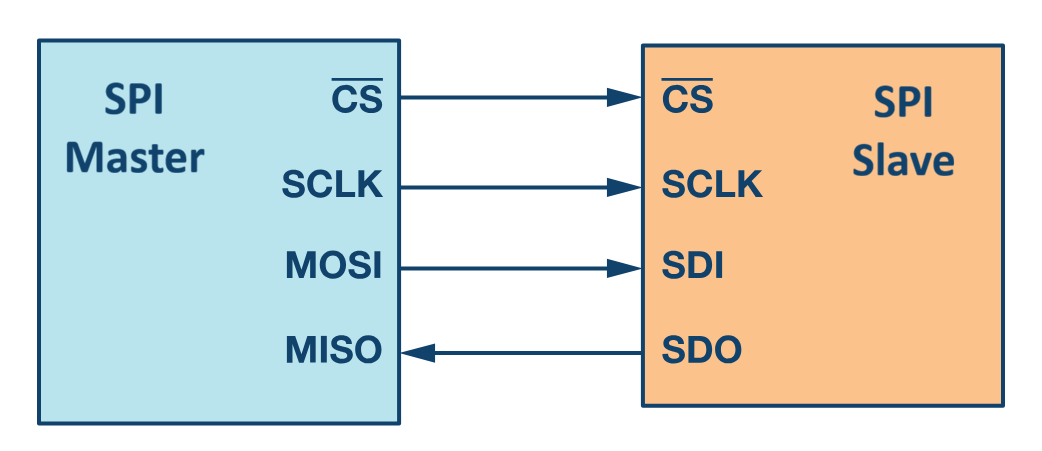
\includegraphics[width = 0.5\textwidth]{media/SPIDiagram.png}
\caption{SPI Configuration of Master and Slave}
\end{figure}

4-wire SPI devices have four signals:
\begin{itemize}
	\item Clock (SPI CLK, SCLK)
    \item Chip select (CS)
    \item Master out, slave in (MOSI)
    \item Master in, slave out (MISO)
\end{itemize}

The device that generates the clock signal is called the master. Data transmitted between the master and the slave is synchronized to the clock generated by the master. SPI devices support much higher clock frequencies compared to I2C interfaces.

The chip select (CS) signal is used by the main device to choose which slave communicates on the SPI bus. It is active low, meaning the slave is selected when the signal is low and disconnected when it is high. If multiple slaves are present, each one needs its own separate chip select line.

MOSI (Master Out Slave In) carries data from the main device to the slave, while MISO (Master In Slave Out) carries data from the slave back to the main device.

\subsection{Data Transmission between the Master and Slave}
To start SPI communication, the master generates the clock signal and selects the slave by pulling the chip select (CS) line low (active low). SPI operates in full-duplex mode, meaning the master and slave can transmit data simultaneously via MOSI and MISO.

During communication, data is shifted out serially while data is also read in at the same time. The clock signal synchronizes this shifting and sampling process. The SPI interface allows flexibility in choosing whether data is sampled or shifted on the rising or falling clock edge. The number of transmitted data bits depends on the specific device. 

\subsection{Clock Polarity and Clock Phase}
In SPI communication, the master configures the clock behavior using two control bits: Clock Polarity (CPOL) and Clock Phase (CPHA). The CPOL bit defines the idle state of the clock signal, i.e., whether the clock remains low (CPOL = 0) or high (CPOL = 1) when no data transmission is taking place. The idle state occurs when the chip select (CS) signal is inactive and at the beginning and end of a transmission.

The CPHA bit determines the clock edge on which data is sampled and shifted. Depending on the configuration, data is captured on either the first or the second clock edge within a clock cycle.

The master must configure CPOL and CPHA according to the timing requirements specified in the slave device’s datasheet. The combination of these two bits results in four possible SPI modes (Mode 0 to Mode 3), each defining a specific clock polarity and phase configuration.

\begin{table}[H]
\begin{tabularx}{\textwidth}{|c|c|c|X|X|}
\hline 
\textbf{SPI Mode} & \textbf{CPOL} & \textbf{CPHA} & \textbf{Clock Polarity in idle state} & \textbf{Clock Phase Used to Sample and/or Shift the Data} \\ \hline 
0 & 0 & 0 & Logic Low & Data sampled on rising edge and shifted out on the falling edge \\ \hline 
1 & 0 & 1 & Logic Low & Data sampled on the falling edge and shifted out on the rising edge \\ \hline
2 & 1 & 0 & Logic High & Data sampled on the falling edge and shifted out on the rising edge \\ \hline
3 & 1 & 1 & Logic High & Data sampled on the rising edge and shifted out on the falling edge \\ \hline
\end{tabularx}
\caption{SPI Modes with CPOL and CPHA}
\end{table}

The following figure illustrate example SPI communication in the four SPI modes, showing data transfer on the MOSI and MISO lines. The start and end of transmission are marked by dotted green lines, while the sampling and shifting edges are indicated in orange and blue, respectively. These figures are provided for illustration only; for reliable SPI communication, the device’s datasheet must be consulted to ensure all timing requirements are satisfied.

\begin{figure}[H]
\centering 
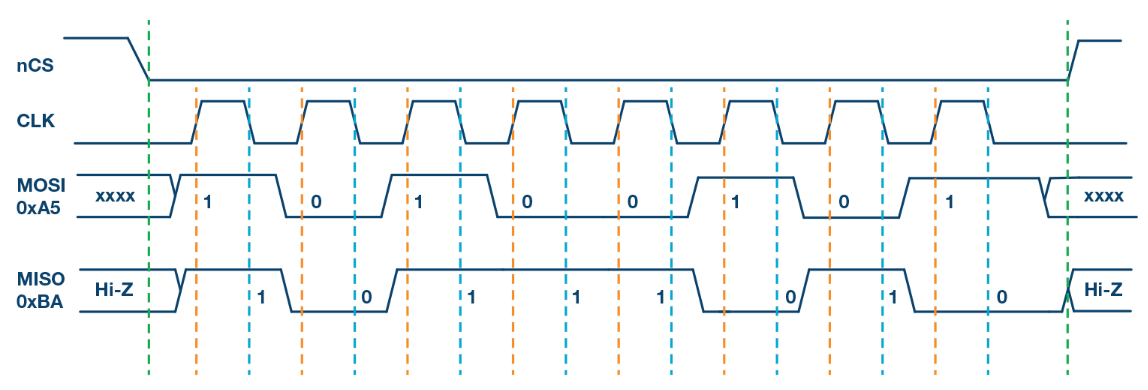
\includegraphics[width = 0.9\textwidth]{media/diagram1.png}
\caption{SPI Mode 0, CPOL = 0, CPHA = 0: CLK idle state = low, data sampled on rising edge and shifted on falling edge}
\label{fig-diagram1}
\end{figure}

 Figure \autoref{fig-diagram2} presents the timing diagram for SPI Mode 1. In this mode, CPOL = 0, meaning the clock remains low during the idle state, and CPHA = 1, meaning data is sampled on the falling clock edge and shifted on the rising clock edge

\begin{figure}[H]
\centering 
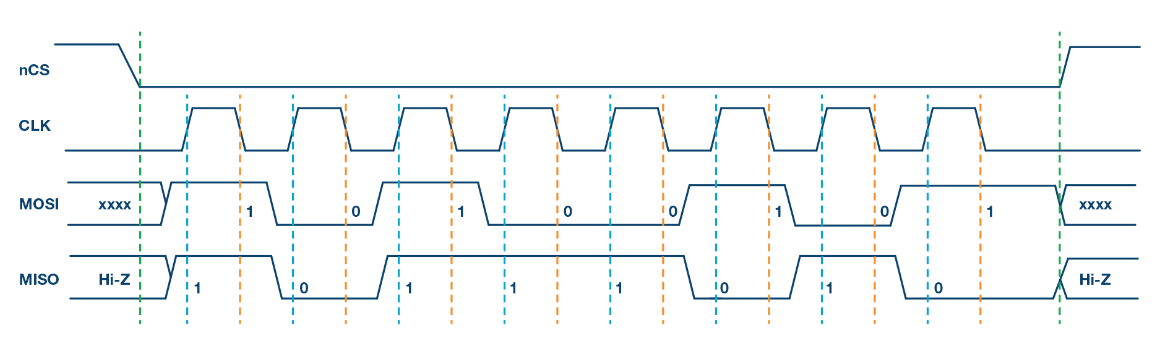
\includegraphics[width = 0.9\textwidth]{media/diagram2.png}
\caption{SPI Mode 1, CPOL = 0, CPHA = 1: CLK idle state = low, data sampled on the falling edge and shifted on the rising edge}
\label{fig-diagram2}
\end{figure}

Figure \ref{fig-diagram3} shows the timing diagram for SPI Mode 2. In this mode, the clock polarity is 1, which indicates that the idle state of the clock signal is high. The clock phase in this mode is 0, which indicates that the data is sampled on the falling edge (shown by the orange dotted line) and the data is shifted on the rising edge (shown by the dotted blue line) of the clock signal.
\begin{figure}[H]
\centering 
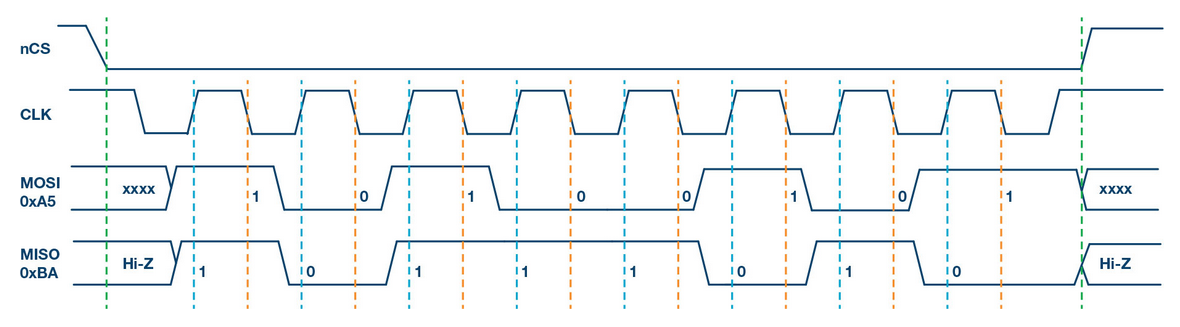
\includegraphics[width = 0.9\textwidth]{media/diagram3.png}
\caption{SPI Mode 2, CPOL = 1, CPHA = 0: CLK idle state = high, data sampled on the falling edge and shifted on the rising edge}
\label{fig-diagram3}
\end{figure}

\autoref{fig-diagram4} shows the timing diagram for SPI Mode 3. In this mode, the clock polarity is 1, which indicates that the idle state of the clock signal is high. The clock phase in this mode is 1, which indicates that the data is sampled on the rising edge (shown by the orange dotted line) and the data is shifted on the falling edge (shown by the dotted blue line) of the clock signal.
\begin{figure}[H]
\centering 
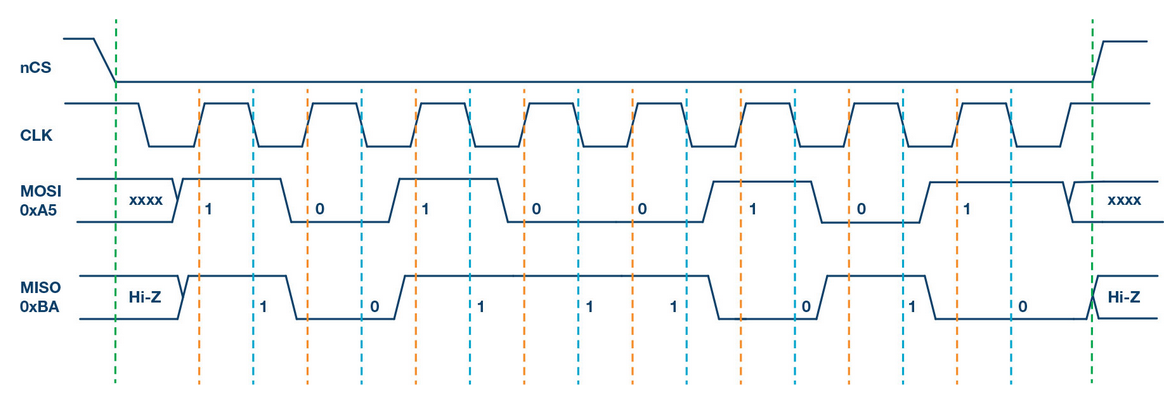
\includegraphics[width = 0.9\textwidth]{media/diagram4.png}
\caption{SPI Mode 3, CPOL = 1, CPHA = 1: CLK idle state = high, data sampled on the rising edge and shifted on the falling edge}
\label{fig-diagram4}
\end{figure}

In SPI systems, a single master can interface with multiple slaves using either a regular or daisy-chain configuration. In the regular mode, each slave requires a dedicated chip select line from the master. When a chip select is pulled low, the corresponding slave is enabled for communication, while enabling multiple slaves simultaneously can corrupt the data on the MISO line. As the number of slaves increases, the number of chip select lines also increases, which may require additional techniques such as multiplexers to manage the connections. In contrast, the daisy-chain configuration connects the slaves in series, allowing data to propagate through each device. This reduces the number of chip select lines needed but increases the number of clock cycles required to reach slaves further down the chain. Each method has trade-offs, and the master must configure the interface according to the specific requirements of the connected slave devices.

\section{SPI in VHDL}
Here in this project we are using an A/D converter, Temperature sensor through the Pmods connectors to the board and the GPIOs present on the Zedboard. \\
for the communication of the A/D converter we need the SPI communication protocol and therefore we need to implment it using VHDL language on the fabric on FPGA. \\
To enable communication between the FPGA and the external A/D converter, the Serial Peripheral Interface (SPI) communication protocol is employed. Since the A/D converter uses SPI as its communication interface, the protocol is implemented directly in VHDL within the programmable logic (FPGA fabric) of the ZedBoard. This approach allows precise timing control and reliable data acquisition without relying on the processing system.\\
The SPI communication protocol is a synchronous serial interface commonly used for short-distance communication between a master device and one or more slave peripherals. In the implemented system, the FPGA operates as the SPI master, while the A/D converter functions as the SPI slave. Communication is initiated and controlled entirely by the master, which generates the clock signal and manages the data transfer sequence.\\
SPI communication is based on four primary signals: Serial Clock (SCLK), Master Out Slave In (MOSI), Master In Slave Out (MISO), and Chip Select (CS). The SCLK signal is generated by the FPGA and defines the timing of data transmission. The MOSI line is used to send control or configuration data from the FPGA to the A/D converter, while the MISO line is used to receive the digitized output data from the converter. The CS signal is used to select and activate the A/D converter during communication, ensuring that data exchange occurs only when intended.\\
The SPI master is implemented in VHDL as a dedicated hardware module. This module generates the required clock signal, controls the chip select line, and manages the serial shifting of data in accordance with the timing requirements specified in the A/D converter datasheet. Data is transmitted and sampled synchronously with the SPI clock, following the defined clock polarity and phase configuration.

A finite state machine (FSM) is used to control the SPI communication process. The FSM manages the different stages of operation, including the idle state, activation of the chip select signal, serial data transmission, data reception, and termination of communication. This structured control mechanism ensures deterministic behavior and reliable data transfer, which are essential for accurate temperature measurement.

Implementing the SPI protocol in FPGA hardware offers several advantages, such as deterministic timing, low latency, and independence from software execution delays. This makes the design well suited for real-time and embedded applications, where consistent and reliable communication with external sensors and converters is required. Additionally, the VHDL-based implementation allows flexibility in adjusting parameters such as clock frequency and data length to support different SPI-compatible devices. \cite{mohammadi-spi-vhdl}

\subsection{SPI master \texttt{CPOL = 0, CPHA = 1}}
The following examples shows the implementation of SPI communication protocol for a master with \texttt{CPO = 0, CPHA = 1}, the example shows the data communication for an 8 bit SPI communication. 
The SPI implementation uses a Finit State Machine that controls the data flow, synchronization logic for SPI clock generation and shift registers for data handling. 

\subsection{Description of the SPI using FSM (Finite State Machine)}
The design implements an SPI (Serial Peripheral Interface) transmitter module configured for mode \texttt{(CPOL = 0, CPHA = 1)} with 8-bit data communication. The design includes a finite state machine (FSM) that manages the different stages of SPI communication: idle, start, data transmission (clock high and low phases), and stop. It uses internal shift registers to handle serial transmission (sdo) and reception (sdi) of data bits. A clock divider is implemented to generate a slower SPI clock \texttt{(spi\_clkp)} derived from the input clock (bclk). The scsq signal acts as the
chip select, active low, and sclk is the SPI clock output. 

\begin{figure}[H]
\centering 
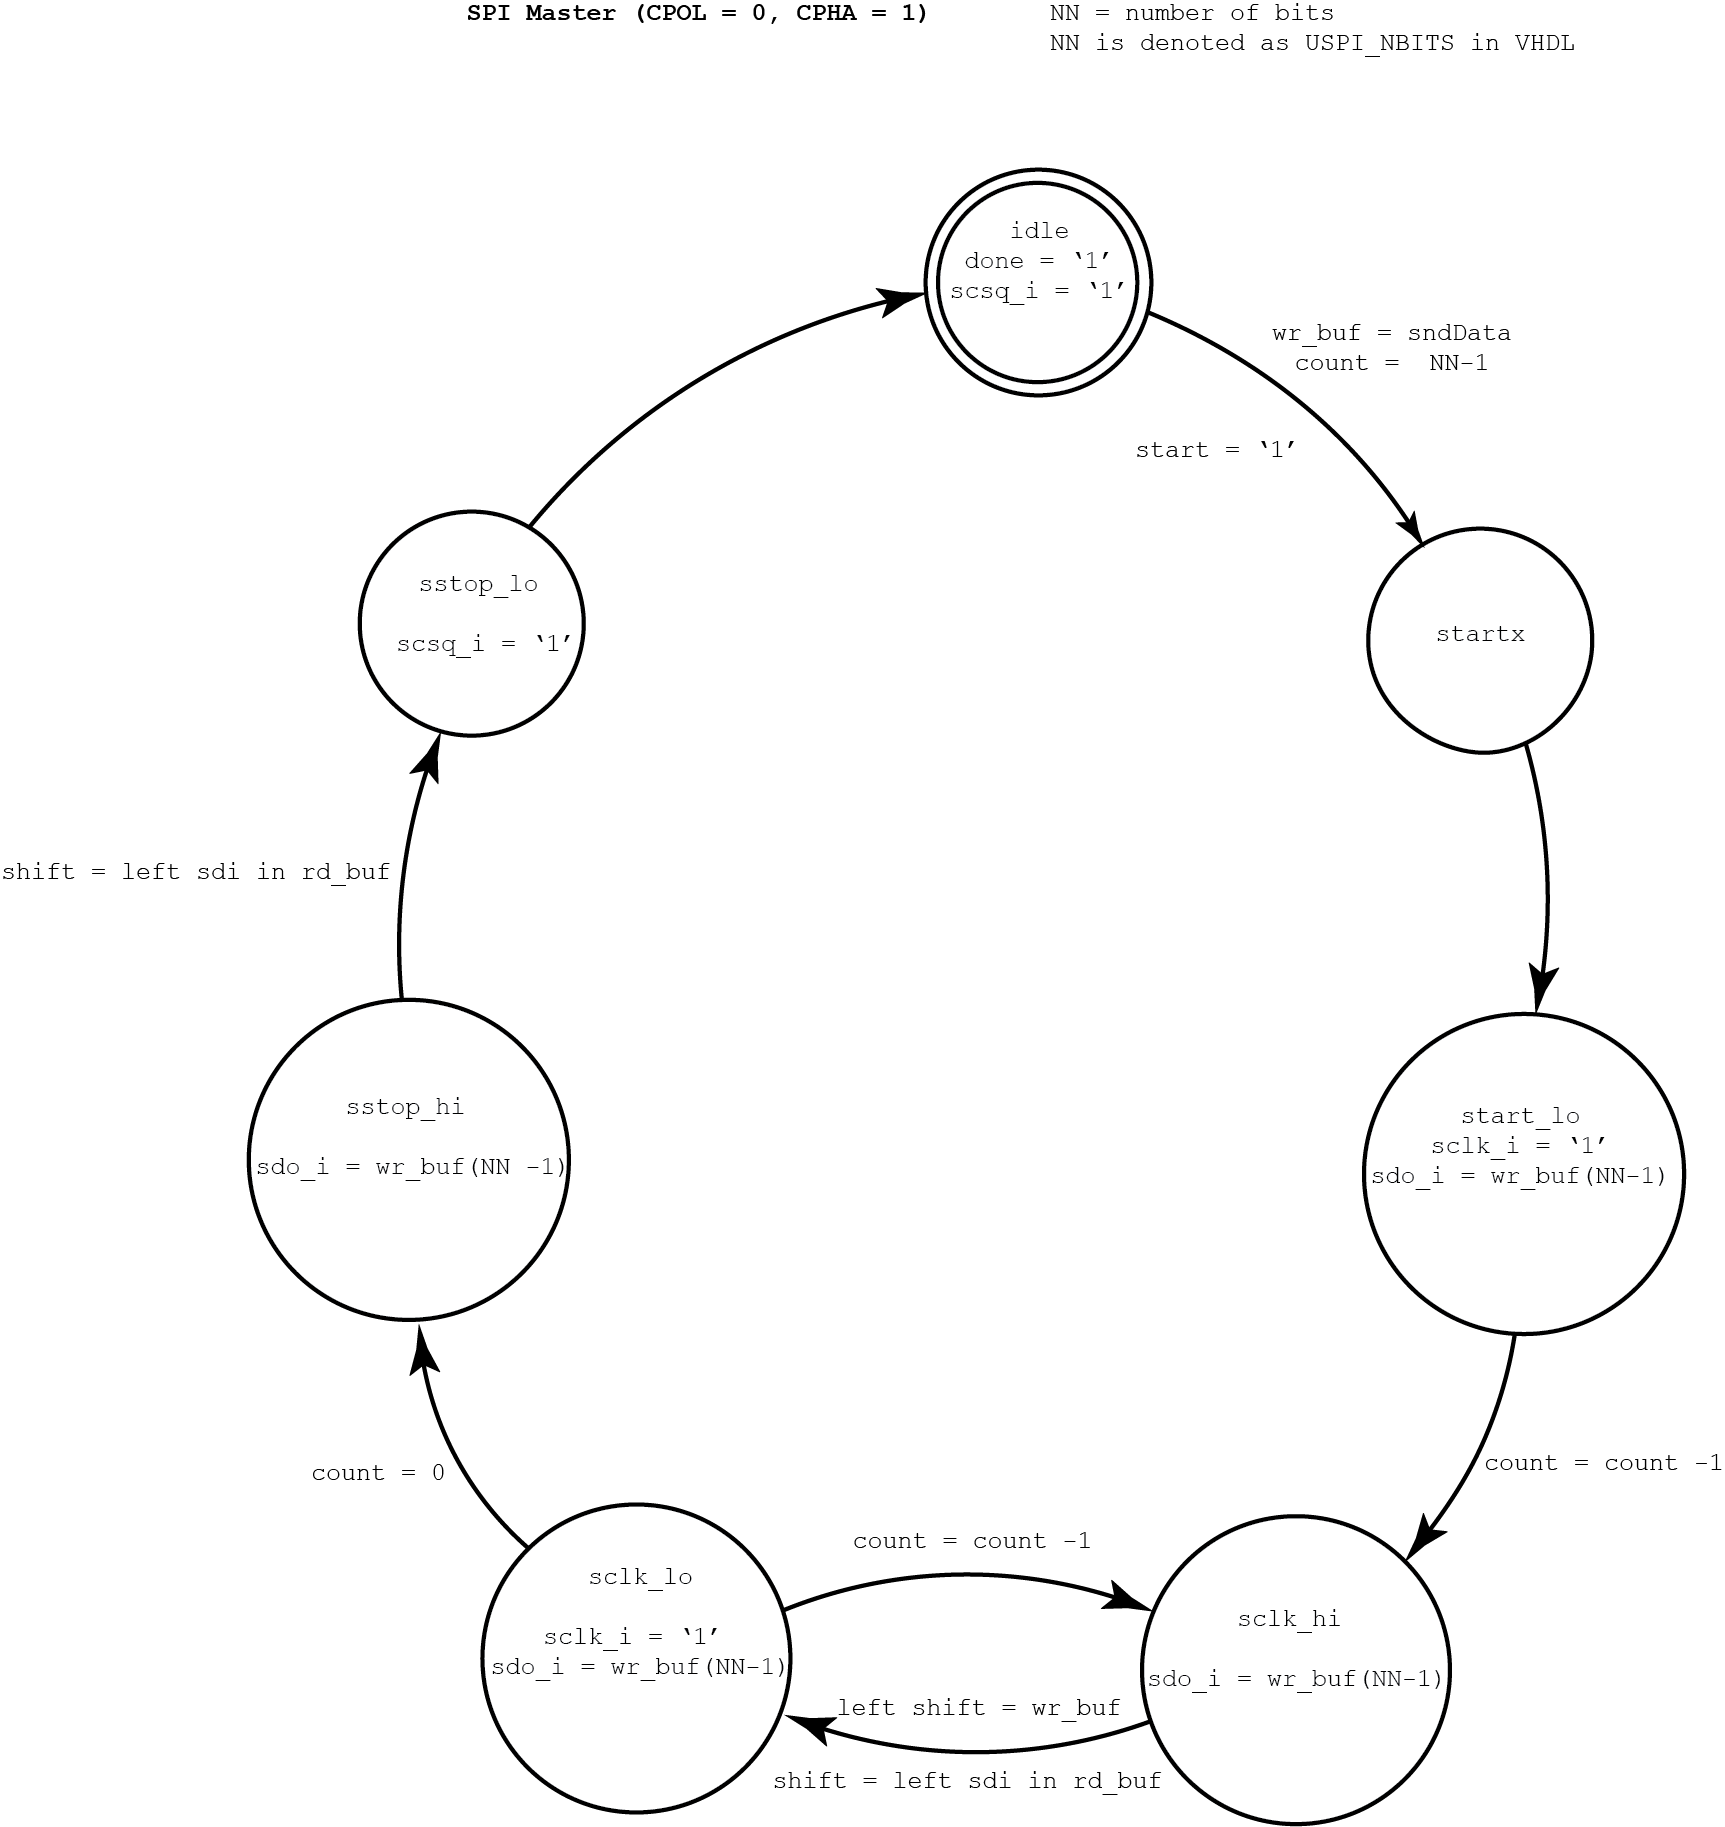
\includegraphics[width = 0.95\textwidth]{media/spi_master.png}
\caption{SPI Master State Machine Diagram}
\label{fig-state_machine}
\end{figure}
The following VHDL codes shows the implementation of the above SPI Master: 
\begin{minted}[bgcolor = lightgray, tabsize = 4, breaklines, numbers = left]{vhdl}
------------------------------------------------------------------------
-- Engineer: Mohammad Mahdi Mohammadi
-- Module Name: spicpol0cph1 - Behavioral
-- Description: SPI transmitter cpol=0, cphase = 1, 8bit.
------------------------------------------------------------------------
LIBRARY IEEE;
USE IEEE.STD_LOGIC_1164.ALL;
ENTITY spicpol0chp1 IS
    PORT (
        reset : IN STD_LOGIC;
        bclk : IN STD_LOGIC;
        start : IN STD_LOGIC;
        done : OUT STD_LOGIC;
        scsq : OUT STD_LOGIC;
        sclk : OUT STD_LOGIC;
        sdi : IN STD_LOGIC;
        sdo : OUT STD_LOGIC;
        sndData : IN STD_LOGIC_VECTOR (7 DOWNTO 0);
        rcvData : OUT STD_LOGIC_VECTOR (7 DOWNTO 0));
END spicpol0chp1;

ARCHITECTURE Behavioral OF spicpol0chp1 IS
    CONSTANT SPI_NBITS : INTEGER := 8;
    TYPE STATE_TYPE IS (sidle, sstartx, sstart_lo, sclk_hi, sclk_lo, sstop_hi, sstop_lo);
    SIGNAL state, next_state : state_type;
    SIGNAL scsq_i, sclk_i, sdo_i : STD_LOGIC;
    SIGNAL lshift : STD_LOGIC;
    SIGNAL start_i : STD_LOGIC;
    SIGNAL wr_buf : STD_LOGIC_VECTOR (SPI_NBITS - 1 DOWNTO 0);
    SIGNAL rd_buf : STD_LOGIC_VECTOR (SPI_NBITS - 1 DOWNTO 0);
    SIGNAL count : INTEGER RANGE 0 TO SPI_NBITS - 1;
    -- for simulation
    CONSTANT clk_div : INTEGER := 3;
    -- for hardware test 5 bits / sec transmission rate
    --constant CLK_DIV : integer := 9999999;
    SUBTYPE counter_type IS INTEGER RANGE 0 TO clk_div;
    SIGNAL SPI_CLKP : STD_LOGIC;
BEGIN
    CLKDIV_P : PROCESS (BCLK)
        VARIABLE cnt : counter_type := clk_div;
    BEGIN
        IF rising_edge (bclk) THEN
            spi_clkp <= '0';
            IF cnt = 0 THEN
                spi_clkp <= '1';
                cnt := clk_div;
            ELSE
                cnt := cnt - 1;
            END IF;
        END IF;
        Complete Source code OF SPI
        8
    END PROCESS clkdiv_p;
    rcvData <= rd_buf;
    seq_p : PROCESS (bclk)
    BEGIN
        IF rising_edge(bclk) THEN
            start_i <= start;
            -- if spi_clkp = '1' then
            IF reset = '1' THEN
                state <= sidle;
                -- scsq <= '0';
                sclk <= '0';
                sdo <= '0';
            ELSE
                IF next_state = sstartx THEN
                    count <= SPI_NBITS - 1;
                    wr_buf <= sndData;
                ELSIF next_state = sclk_hi THEN
                    count <= count - 1;
                ELSIF next_state = sclk_lo THEN
                    wr_buf <= wr_buf(SPI_NBITS - 2 DOWNTO 0) & '-';
                    rd_buf <= rd_buf(SPI_NBITS - 2 DOWNTO 0) & sdi;
                ELSIF next_state = sstop_lo THEN
                    rd_buf <= rd_buf(SPI_NBITS - 2 DOWNTO 0) & sdi;
                END IF;
                state <= next_state;
                scsq <= scsq_i;
                sclk <= sclk_i;
                sdo <= sdo_i;
                -- end if;
            END IF;
        END IF;
    END PROCESS seq_p;

    cmb_p : PROCESS (state, start_i, count, wr_buf)
    BEGIN
        next_state <= state;
        scsq_i <= '0';
        sclk_i <= '0';
        sdo_i <= '0';
        done <= '0';
        CASE state IS
            WHEN sidle =>
                done <= '1';
                scsq_i <= '1';
                IF start_i = '1' THEN
                    next_state <= sstartx;
                END IF;
            WHEN sstartx =>
                next_state <= sstart_lo;
            WHEN sstart_lo =>
                sclk_i <= '1';
                sdo_i <= wr_buf(SPI_NBITS - 1);
                next_state <= sclk_hi;
            WHEN sclk_hi =>
                sdo_i <= wr_buf(SPI_NBITS - 1);
                next_state <= sclk_lo;
            WHEN sclk_lo =>
                sclk_i <= '1';
                sdo_i <= wr_buf(SPI_NBITS - 1);
                IF count = 0 THEN
                    next_state <= sstop_hi;
                ELSE
                    next_state <= sclk_hi;
                END IF;
            WHEN sstop_hi =>
                Top Level FILE
                9
                sdo_i <= wr_buf(SPI_NBITS - 1);
                next_state <= sstop_lo;
            WHEN sstop_lo =>
                scsq_i <= '1';
                next_state <= sidle;
        END CASE;
    END PROCESS cmb_p;
END Behavioral;
\end{minted}

\section{Section 2: Hardware Design of Measurement Network Gateway}
	One of the most important part of this project is the use of Embedded Linux in zynq7000 FPGA on ZedBoard Evaluation Board. The hardware required for this project is developed inside Vivado in VHDL language.\\
	The system shall acquire data from a precision resistive temperature sensor, two ADCs, onboard Switches and Push Buttons. \\
	For this reason a new custom AXI slave IP has been created inside Vivado and this Ip has the following hierarchy structure.
	\begin{figure}[H]
	\begin{center}
	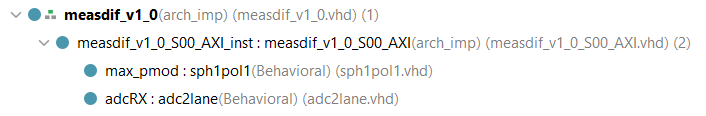
\includegraphics[width = 0.75\textwidth]{media/hstructure.png}
	\caption{Hierarchy Structure of the Custom AXI slave IP in Vivado}
	\end{center}
	\end{figure} 
	\subsection{Description of the file: adc2lane.vhd}
	This file is made to acquire data from two ADCs based on SPI (CPOL=0, CPHA=1) communication protocal. \\
	The entity adc2lane is a configurable SPI receiver that operates with two input data channels (sdi\_0 and sdi\_1) in parallel, capturing data words of configurable length (USPI\_SIZE, default 16 bits). It communicates synchronously using SPI mode settings CPOL=0 and CPHA=1.
	The following is the VHDL code for the implemenation of acquiring data from the ADCs using SPI. 
	
	\textbf{Inputs:}
	\begin{enumerate}
	\item resetn: Active-low synchronous reset.
	\item bclk: Base clock for FSM timing.
	\item spi\_clkp: SPI clock polarity indicator (CPOL=0 here).
	\item start: Signal to begin data acquisition.
	\item sdi\_0, sdi\_1: Serial data inputs from two ADC lanes.
	\end{enumerate}
	\textbf{Outputs:}
	\begin{enumerate}
	\item done: Signal asserted when data reception is complete.
	\item scsq: SPI chip select line, active low.
	\item sclk: SPI clock output.
	\item rcvData\_0, rcvData\_1: Received data vectors from both SPI lanes.
	\end{enumerate}
	At the beginning of the VHDL program, the standard libraries are used: 
\begin{minted}[breaklines, tabsize = 4, bgcolor = lightgray]{VHDL}
library IEEE;
use IEEE.STD_LOGIC_1164.ALL;
\end{minted}

are included to make standard logic types and definitions available for the design. The library IEEE; statement declares the use of the IEEE library, which contains commonly used packages, while use \texttt{IEEE.STD\_LOGIC\_1164.ALL;} imports all definitions from the \texttt{STD\_LOGIC\_1164} package.
	
This package provides the std\_logic and std\_logic\_vector types, which support multiple logic values (such as 0, 1, Z, and X) and are essential for modeling digital signals and buses. Including these lines ensures that the designer can use standard logic data types and operations throughout the VHDL code.\\

After adding the standard libraries, the input and output of the IP is defined as follows:
\begin{minted}[breaklines, tabsize = 4, bgcolor = lightgray]{VHDL}
entity adc2lane is
    GENERIC ( USPI_SIZE : INTEGER := 16 );
    Port ( resetn : in STD_LOGIC;
       bclk : in STD_LOGIC;
       spi_clkp : in STD_LOGIC;
       start : in STD_LOGIC;
       done : out STD_LOGIC;
       scsq : out STD_LOGIC;
       sclk : out STD_LOGIC;
       sdi_0 : in STD_LOGIC;
       sdi_1 : in STD_LOGIC;
       rcvData_0 : out STD_LOGIC_VECTOR (USPI_SIZE-1 downto 0);
       rcvData_1 : out STD_LOGIC_VECTOR (USPI_SIZE-1 downto 0));
end adc2lane;
\end{minted}
 
In this VHDL design, custom enumerated types are defined to represent the states of two finite state machines (FSMs). The type \texttt{state\_type} defines six states (\texttt{sidle}, \texttt{sstartx}, \texttt{sclk\_lo}, \texttt{sclk\_hi}, \texttt{sstop\_lo}, \texttt{sstop\_hi}) for controlling the SPI clock and data transmission, with corresponding signals \texttt{state} and \texttt{next\_state} used to hold the current and next states. The SPI signals \texttt{sclk\_i} and \texttt{scsq\_i} are declared as \texttt{STD\_LOGIC}, while two read buffers, \texttt{rd\_buf\_0} and \texttt{rd\_buf\_1}, are defined as \texttt{STD\_LOGIC\_VECTOR} arrays of size \texttt{USPI\_SIZE}. A counter signal \texttt{count} is used to track the bit position during SPI transfers. Additionally, a second FSM for slave select control is defined using the type \texttt{sslst\_type} with three states (\texttt{ssl\_idle}, \texttt{ssl\_start}, \texttt{ssl\_run}), with \texttt{ssl\_state} and \texttt{sslnxt\_state} representing the current and next states. The signal \texttt{start\_i} acts as an input trigger for initiating the slave select sequence. This structured use of enumerated types and signals ensures clear and organized control over the SPI communication process.

\begin{minted}[breaklines, tabsize = 4, bgcolor = lightgray]{VHDL}
architecture Behavioral of adc2lane is

type state_type IS (sidle, sstartx, sclk_lo, sclk_hi, sstop_lo, sstop_hi);
SIGNAL  state, next_state: state_type;
SIGNAL sclk_i, scsq_i : STD_LOGIC;
SIGNAL rd_buf_0, rd_buf_1 : STD_LOGIC_VECTOR(USPI_SIZE-1 downto 0);
SIGNAL count : integer RANGE 0 TO USPI_SIZE-1;

type sslst_type IS (ssl_idle, ssl_start, ssl_run);
SIGNAL ssl_state, sslnxt_state: sslst_type;
SIGNAL start_i : STD_LOGIC;
\end{minted}

The following assignment:
\begin{minted}[breaklines, tabsize = 4, bgcolor = lightgray]{VHDL}
begin

    rcvData_0 <= rd_buf_0;
    rcvData_1 <= rd_buf_1;
\end{minted}

are used to transfer the contents of the internal read buffers to the output signals. Here, \texttt{rd\_buf\_0} and \texttt{rd\_buf\_1} hold the data received from the SPI interface, and by assigning them to \texttt{rcvData\_0} and \texttt{rcvData\_1}, the received data is made available for use in other parts of the design or for further processing. This ensures that the SPI data captured in the buffers is properly output from the module while maintaining synchronization with the system clock.


\begin{minted}[breaklines, tabsize = 4, bgcolor = lightgray]{VHDL}
	-- start/stop logic
	-- proper handling of clock division
	sslseq_proc: PROCESS(resetn, bclk, sslnxt_state)
	BEGIN
		IF rising_edge(bclk) THEN
			IF resetn='0' THEN
				ssl_state <= ssl_idle;
			ELSE
				ssl_state <= sslnxt_state;
			END IF;
		END IF;
	END PROCESS sslseq_proc;
\end{minted}

The \texttt{sslseq\_proc} process implements a finite state machine (FSM) to control the SPI slave select (SS) signal. It updates the current state (\texttt{ssl\_state}) synchronously on the rising edge of the base clock (\texttt{bclk}) and can be reset to the idle state (\texttt{ssl\_idle}) when \texttt{resetn} is low, ensuring the slave is properly deselected on system reset. By sequencing through defined states such as idle, start, and run, the process determines when the slave is selected and for how long, effectively controlling the timing of the SS signal. The FSM can remain in a particular state for multiple clock cycles, which produces a clock division effect that guarantees the slave is enabled for the correct duration during SPI data transfers. This structure ensures precise, clock-synchronized selection and deselection of the slave device, providing reliable SPI communication without requiring additional timing hardware.



\begin{minted}[breaklines, tabsize = 4, bgcolor = lightgray]{VHDL}
	sslcmb_proc: PROCESS(ssl_state, state, start)
	BEGIN
		sslnxt_state <= ssl_state;
		start_i <= '0';
		done <= '0';
		CASE ssl_state IS
			WHEN ssl_idle =>
				done <= '1';
				IF start='1' AND state=sidle THEN
					sslnxt_state <= ssl_start;
				END IF;
			WHEN ssl_start =>
				start_i <= '1';
				IF state=sstartx THEN
					sslnxt_state <= ssl_run;
				END IF;
			WHEN ssl_run =>
				IF state=sidle THEN
					sslnxt_state <= ssl_idle;
				END IF;
		END CASE;
	END PROCESS sslcmb_proc;
\end{minted}

The \texttt{sslcmb\_proc} process implements the combinational logic for the slave select finite state machine (FSM) in the SPI interface. It determines the next state (\texttt{sslnxt\_state}) and controls the output signals \texttt{start\_i} and \texttt{done} based on the current FSM state (\texttt{ssl\_state}), the SPI transmission state (\texttt{state}), and the \texttt{start} input signal. In the idle state (\texttt{ssl\_idle}), \texttt{done} is set to \textquotesingle 1\textquotesingle{} to indicate that the SPI transmission is finished, and if \texttt{start} = \textquotesingle 1\textquotesingle{} while the SPI FSM is idle (\texttt{sidle}), the FSM transitions to \texttt{ssl\_start}. In the \texttt{ssl\_start} state, \texttt{start\_i} is set to \textquotesingle 1\textquotesingle{} to initiate the slave select activation, and once the SPI FSM reaches the \texttt{sstartx} state, the FSM moves to \texttt{ssl\_run}. During \texttt{ssl\_run}, the slave select signal remains active while data is being transferred, and the FSM returns to \texttt{ssl\_idle} once the SPI FSM returns to \texttt{sidle}. This process ensures proper timing and sequencing of the slave select signal, coordinating its activation and deactivation with the SPI transmission without requiring additional sequential logic.



\begin{minted}[breaklines, tabsize = 4, bgcolor = lightgray]{VHDL}
	-- spi logic
	sseq_proc: PROCESS(resetn, bclk, next_state, sclk_i, scsq_i,
				       rd_buf_0, rd_buf_0, sdi_0, sdi_1, count, spi_clkp)
	BEGIN
		IF rising_edge(bclk) THEN
			IF resetn='0' THEN
				state <= sidle;
				count <= USPI_SIZE-1;
			ELSIF spi_clkp='1' THEN
				IF next_state=sstartx THEN
                count <= USPI_SIZE - 1;
                ELSIF next_state=sclk_lo THEN
                    count <= count - 1;
                    rd_buf_0 <= rd_buf_0(USPI_SIZE-2 downto 0) & sdi_0;
                    rd_buf_1 <= rd_buf_1(USPI_SIZE-2 downto 0) & sdi_1;
                ELSIF next_state=sstop_lo THEN
                    rd_buf_0 <= rd_buf_0(USPI_SIZE-2 downto 0) & sdi_0;
                    rd_buf_1 <= rd_buf_1(USPI_SIZE-2 downto 0) & sdi_1;
                END IF;
                state <= next_state;
                sclk <= sclk_i;
                scsq <= scsq_i;
			END IF;
		END IF;
	END PROCESS sseq_proc;
\end{minted}

The \texttt{sseq\_proc} process implements the main SPI logic, managing both the data reception and the finite state machine (FSM) that controls the SPI interface. It operates synchronously on the rising edge of the base clock (\texttt{bclk}) and responds to the reset signal (\texttt{resetn}) and the SPI clock enable signal (\texttt{spi\_clkp}). When the reset is active (\texttt{resetn = '0'}), the FSM state is initialized to \texttt{sidle} and the bit counter is set to \texttt{USPI\_SIZE-1}, ensuring that the SPI interface starts in a known idle state.

During normal operation, the process monitors the FSM states to control data reception and state transitions. In the \texttt{sstartx} state, the bit counter is reset to prepare for receiving a new SPI word. In the \texttt{sclk\_lo} state, the counter decrements for each clock cycle, and the incoming serial data bits (\texttt{sdi\_0} and \texttt{sdi\_1}) are shifted into the read buffers (\texttt{rd\_buf\_0} and \texttt{rd\_buf\_1}), performing serial-to-parallel conversion. In the \texttt{sstop\_lo} state, the final bits of the SPI word are shifted into the buffers to complete the data reception.

At each enabled clock cycle, the FSM updates the current state to the next state (\texttt{next\_state}), while the SPI clock (\texttt{sclk}) and slave select clock (\texttt{scsq}) signals are updated from their internal signals (\texttt{sclk\_i} and \texttt{scsq\_i}). This process ensures proper timing and sequencing of the SPI FSM, accurate serial-to-parallel conversion of received data, and synchronized control of the SPI clock and slave select signals, enabling reliable SPI communication.


\begin{minted}[breaklines, tabsize = 4, bgcolor = lightgray]{VHDL}
	scmb_proc: PROCESS(state, start_i, count)
	BEGIN
		next_state <= state;
		sclk_i <= '1';
		scsq_i <= '0';
		CASE state IS
			WHEN sidle =>
				scsq_i <= '1';
				IF start_i='1' THEN
					next_state <= sstartx;
				END IF;
			WHEN sstartx =>
                next_state <= sclk_hi;
			WHEN sclk_hi =>
                sclk_i <= '0';
                IF count=0 THEN
                    next_state <= sstop_lo;
                ELSE
                    next_state <= sclk_lo;
                END IF;
            WHEN sclk_lo =>
				next_state <= sclk_hi;
			WHEN sstop_lo =>
				next_state <= sstop_hi;
			WHEN sstop_hi =>
				scsq_i <= '1';
				next_state <= sidle;
		END CASE;
	END PROCESS scmb_proc;

end Behavioral;
\end{minted}

The \texttt{scmb\_proc} process implements the combinational logic for controlling the SPI clock (\texttt{sclk\_i}) and slave select (\texttt{scsq\_i}) signals based on the current FSM state (\texttt{state}), the start signal (\texttt{start\_i}), and the bit counter (\texttt{count}). In the idle state (\texttt{sidle}), the slave select is high, and if \texttt{start\_i} is active, the FSM moves to \texttt{sstartx} to begin a transaction. The FSM then alternates between \texttt{sclk\_hi} and \texttt{sclk\_lo} to generate clock pulses, using the bit counter to determine when the data transfer is complete. After the last bit, the FSM transitions through \texttt{sstop\_lo} and \texttt{sstop\_hi}, sets the slave select high, and returns to \texttt{sidle}, completing the SPI transaction. This process ensures correct clock generation, slave selection, and sequencing for reliable SPI communication.\\

Here is the complete VHDL code for this program. 
\begin{minted}[breaklines, tabsize = 4, bgcolor = lightgray, numbers=left]{VHDL}
----------------------------------------------------------------------------------
-- Company:         Univ. Bremerhaven
-- Engineer:        Kai Mueller
-- 
-- Create Date:     08.06.2016 00:15:32
-- Description:     ADC 2 Lanes SPI based on spipol1pha0 template (CPOL=0 CPHA=1)
-- 
----------------------------------------------------------------------------------

library IEEE;
use IEEE.STD_LOGIC_1164.ALL;

entity adc2lane is
    GENERIC ( USPI_SIZE : INTEGER := 16 );
    Port ( resetn : in STD_LOGIC;
       bclk : in STD_LOGIC;
       spi_clkp : in STD_LOGIC;
       start : in STD_LOGIC;
       done : out STD_LOGIC;
       scsq : out STD_LOGIC;
       sclk : out STD_LOGIC;
       sdi_0 : in STD_LOGIC;
       sdi_1 : in STD_LOGIC;
       rcvData_0 : out STD_LOGIC_VECTOR (USPI_SIZE-1 downto 0);
       rcvData_1 : out STD_LOGIC_VECTOR (USPI_SIZE-1 downto 0));
end adc2lane;

architecture Behavioral of adc2lane is

type state_type IS (sidle, sstartx, sclk_lo, sclk_hi, sstop_lo, sstop_hi);
SIGNAL  state, next_state: state_type;
SIGNAL sclk_i, scsq_i : STD_LOGIC;
SIGNAL rd_buf_0, rd_buf_1 : STD_LOGIC_VECTOR(USPI_SIZE-1 downto 0);
SIGNAL count : integer RANGE 0 TO USPI_SIZE-1;

type sslst_type IS (ssl_idle, ssl_start, ssl_run);
SIGNAL ssl_state, sslnxt_state: sslst_type;
SIGNAL start_i : STD_LOGIC;

begin

    rcvData_0 <= rd_buf_0;
    rcvData_1 <= rd_buf_1;

	-- start/stop logic
	-- proper handling of clock division
	sslseq_proc: PROCESS(resetn, bclk, sslnxt_state)
	BEGIN
		IF rising_edge(bclk) THEN
			IF resetn='0' THEN
				ssl_state <= ssl_idle;
			ELSE
				ssl_state <= sslnxt_state;
			END IF;
		END IF;
	END PROCESS sslseq_proc;

	sslcmb_proc: PROCESS(ssl_state, state, start)
	BEGIN
		sslnxt_state <= ssl_state;
		start_i <= '0';
		done <= '0';
		CASE ssl_state IS
			WHEN ssl_idle =>
				done <= '1';
				IF start='1' AND state=sidle THEN
					sslnxt_state <= ssl_start;
				END IF;
			WHEN ssl_start =>
				start_i <= '1';
				IF state=sstartx THEN
					sslnxt_state <= ssl_run;
				END IF;
			WHEN ssl_run =>
				IF state=sidle THEN
					sslnxt_state <= ssl_idle;
				END IF;
		END CASE;
	END PROCESS sslcmb_proc;

	-- spi logic
	sseq_proc: PROCESS(resetn, bclk, next_state, sclk_i, scsq_i,
				       rd_buf_0, rd_buf_0, sdi_0, sdi_1, count, spi_clkp)
	BEGIN
		IF rising_edge(bclk) THEN
			IF resetn='0' THEN
				state <= sidle;
				count <= USPI_SIZE-1;
			ELSIF spi_clkp='1' THEN
				IF next_state=sstartx THEN
                count <= USPI_SIZE - 1;
                ELSIF next_state=sclk_lo THEN
                    count <= count - 1;
                    rd_buf_0 <= rd_buf_0(USPI_SIZE-2 downto 0) & sdi_0;
                    rd_buf_1 <= rd_buf_1(USPI_SIZE-2 downto 0) & sdi_1;
                ELSIF next_state=sstop_lo THEN
                    rd_buf_0 <= rd_buf_0(USPI_SIZE-2 downto 0) & sdi_0;
                    rd_buf_1 <= rd_buf_1(USPI_SIZE-2 downto 0) & sdi_1;
                END IF;
                state <= next_state;
                sclk <= sclk_i;
                scsq <= scsq_i;
			END IF;
		END IF;
	END PROCESS sseq_proc;

	scmb_proc: PROCESS(state, start_i, count)
	BEGIN
		next_state <= state;
		sclk_i <= '1';
		scsq_i <= '0';
		CASE state IS
			WHEN sidle =>
				scsq_i <= '1';
				IF start_i='1' THEN
					next_state <= sstartx;
				END IF;
			WHEN sstartx =>
                next_state <= sclk_hi;
			WHEN sclk_hi =>
                sclk_i <= '0';
                IF count=0 THEN
                    next_state <= sstop_lo;
                ELSE
                    next_state <= sclk_lo;
                END IF;
            WHEN sclk_lo =>
				next_state <= sclk_hi;
			WHEN sstop_lo =>
				next_state <= sstop_hi;
			WHEN sstop_hi =>
				scsq_i <= '1';
				next_state <= sidle;
		END CASE;
	END PROCESS scmb_proc;

end Behavioral;
\end{minted}

\subsection{Description of the file: sph1pol1.vhd}
The VHDL module implements an SPI master used to interface with the MAX31865 Pmod. The MAX31865 converts the resistance of an RTD sensor into a digital value accessible via SPI. Communication is initiated by asserting the start signal, which triggers the internal FSM to activate the chip select (scsq) and begin serial data transfer.

Input data (sndData) containing register addresses or commands is loaded into an internal shift register (wr\_buf) and transmitted bit by bit on sdo, while incoming bits from sdi are captured in rd\_buf. A counter ensures all USPI\_SIZE bits are transferred. After the transaction, scsq is deactivated and the received data is available on rcvData, representing the RTD measurement.

The SPI clock (sclk) idle state corresponds to CPOL = 1, and data shifting and sampling occur in alternating clock phases as defined by the FSM. This design provides a reliable, FSM-based SPI master capable of configuring and reading the MAX31865 Pmod.\\
It exposes the following ports:\\
\textbf{Inputs:}
\begin{enumerate}
\item resetn: Active-low reset signal for synchronous initialization.
\item bclk: Base clock signal used to drive internal FSM timing.
\item spi\_clkp: Indicates the SPI clock polarity (CPOL=1 in this design).
\item start: Initiates an SPI transaction.
\item sdi: Serial data input from the slave device.
\item sndData: Data vector to be transmitted through MOSI.
\end{enumerate}
\textbf{outputs:}
\begin{enumerate}
\item done: Signal asserted at the completion of an SPI transaction.
\item scsq: Chip select output, active low for SPI device enabling.
\item sclk: SPI clock output.
\item sdo: Serial data output to the slave device.
\item rcvData: Received data vector collected from MISO.
\end{enumerate}

\begin{minted}[breaklines, tabsize = 4, bgcolor = lightgray]{VHDL}
library IEEE;
use IEEE.STD_LOGIC_1164.ALL;

entity sph1pol1 is
    GENERIC ( USPI_SIZE : INTEGER := 16 );
    Port ( resetn : in STD_LOGIC;
            bclk : in STD_LOGIC;
            spi_clkp : in STD_LOGIC;
            start : in STD_LOGIC;
            done : out STD_LOGIC;
            scsq : out STD_LOGIC;
            sclk : out STD_LOGIC;
            sdo : out STD_LOGIC;
            sdi : in STD_LOGIC;
            sndData : in STD_LOGIC_VECTOR (USPI_SIZE-1 downto 0);
            rcvData : out STD_LOGIC_VECTOR (USPI_SIZE-1 downto 0));
end sph1pol1;
\end{minted}

The standard IEEE library is included in this module, and the package \texttt{STD\_LOGIC\_1164.ALL} is imported to provide the required data types such as \texttt{STD\_LOGIC} and \texttt{STD\_LOGIC\_VECTOR}, which are essential for modeling digital signals and multi-bit buses in VHDL.

After including the necessary libraries, the entity \texttt{sph1pol1} is declared to define the external interface of the module. A generic parameter \texttt{USPI\_SIZE : INTEGER := 16} is introduced to configure the SPI data width, allowing flexible word lengths during instantiation.
 
The input ports include \texttt{resetn} as an active-low reset signal, \texttt{bclk} as the base clock, \texttt{spi\_clkp} for SPI clock polarity control, \texttt{start} to initiate transmission, \texttt{sdi} as the serial data input (MISO), and \texttt{sndData} as the parallel data to be transmitted. The output ports include \texttt{done} to indicate completion of transmission, \texttt{scsq} as the chip select signal, \texttt{sclk} as the SPI clock output, \texttt{sdo} as the serial data output (MOSI), and \texttt{rcvData} as the parallel received data. Altogether, this entity defines a configurable SPI master interface capable of transmitting and receiving data words of adjustable length using a simple start--done handshake mechanism.


\begin{minted}[breaklines, tabsize = 4, bgcolor = lightgray]{VHDL}
architecture Behavioral of sph1pol1 is

type state_type IS (sidle, sstartx, sstart_lo, sclk_lo, sclk_hi, stop_hi, stop_lo);
SIGNAL  state, next_state: state_type;
SIGNAL sclk_i, scsq_i, sdo_i : STD_LOGIC;
SIGNAL wr_buf : STD_LOGIC_VECTOR(USPI_SIZE-1 downto 0);
SIGNAL rd_buf : STD_LOGIC_VECTOR(USPI_SIZE-1 downto 0);
SIGNAL count : integer RANGE 0 TO USPI_SIZE-1;

type sslst_type IS (ssl_idle, ssl_start, ssl_run);
SIGNAL ssl_state, sslnxt_state: sslst_type;
SIGNAL start_i : STD_LOGIC;
\end{minted}
In this part of the design, the internal signals and state machines required for SPI communication with the MAX31865 are defined. The first finite state machine (FSM), represented by \texttt{state\_type}, handles the bit-level SPI operations. It controls the chip select, generates the SPI clock, shifts out commands or data through \texttt{sdo\_i}, and reads incoming bits from \texttt{sdi} into the receive buffer \texttt{rd\_buf}. The signal \texttt{count} keeps track of how many bits have been transmitted or received, ensuring that a full \texttt{USPI\_SIZE}-bit word is transferred. The transmit buffer \texttt{wr\_buf} holds the command or configuration data sent to the MAX31865, while \texttt{rd\_buf} stores the sensor's response, including the RTD measurement.

The second FSM, represented by \texttt{sslst\_type}, manages the overall transaction flow. It synchronizes the \texttt{start} signal and ensures that SPI transfers only begin when requested, asserting the \texttt{done} signal when the transaction completes. Together, these FSMs and signals allow the SPI master to reliably configure the MAX31865 and read temperature measurements from the RTD sensor.

\begin{minted}[breaklines, tabsize = 4, bgcolor = lightgray]{VHDL}
begin

	rcvData <= rd_buf;

	-- start/stop logic
	-- proper handling of clock division
	sslseq_proc: PROCESS(resetn, bclk, sslnxt_state)
	BEGIN
		IF rising_edge(bclk) THEN
			IF resetn='0' THEN
				ssl_state <= ssl_idle;
			ELSE
				ssl_state <= sslnxt_state;
			END IF;
		END IF;
	END PROCESS sslseq_proc;
\end{minted}
This part of the code assigns the internal receive buffer \texttt{rd\_buf} to \texttt{rcvData} and updates the start/stop FSM (\texttt{ssl\_state}). On each rising edge of \texttt{bclk}, the FSM resets to \texttt{ssl\_idle} if \texttt{resetn} is low; otherwise, it transitions to the next state (\texttt{sslnxt\_state}), ensuring that SPI transactions remain synchronized with the system clock.

\begin{minted}[bgcolor=lightgray, tabsize=4, breaklines]{vhdl}
	sslcmb_proc: PROCESS(ssl_state, state, start)
	BEGIN
		sslnxt_state <= ssl_state;
		start_i <= '0';
		done <= '0';
		CASE ssl_state IS
			WHEN ssl_idle =>
				done <= '1';
				IF start='1' AND state=sidle THEN
					sslnxt_state <= ssl_start;
				END IF;
			WHEN ssl_start =>
				start_i <= '1';
				IF state=sstartx THEN
					sslnxt_state <= ssl_run;
				END IF;
			WHEN ssl_run =>
				IF state=sidle THEN
					sslnxt_state <= ssl_idle;
				END IF;
		END CASE;
	END PROCESS sslcmb_proc;
\end{minted}
The process \texttt{sslcmb\_proc} implements the combinational logic for the start/stop FSM controlling SPI transactions. It determines the next state (\texttt{sslnxt\_state}) based on the current FSM state (\texttt{ssl\_state}), the main SPI state (\texttt{state}), and the external \texttt{start} signal. In the idle state (\texttt{ssl\_idle}), the \texttt{done} signal is asserted, and if \texttt{start} is high while the SPI is idle, the FSM transitions to \texttt{ssl\_start}. In \texttt{ssl\_start}, the internal \texttt{start\_i} signal is asserted to initiate the SPI transfer, and when the SPI FSM enters \texttt{sstartx}, the FSM moves to \texttt{ssl\_run}. In \texttt{ssl\_run}, the FSM returns to idle when the SPI FSM completes the transfer (\texttt{state = sidle}). This logic ensures that SPI transfers start only when requested and properly signal completion.

\begin{minted}[bgcolor= lightgray, tabsize=4, breaklines]{vhdl}
	-- spi logic
	sseq_proc: PROCESS(bclk)
	BEGIN
		IF rising_edge(bclk) THEN
			IF resetn='0' THEN
				state <= sidle;
				count <= USPI_SIZE-1;
			ELSIF spi_clkp='1' THEN
				IF next_state=sstartx THEN
                wr_buf <= sndData;
                count <= USPI_SIZE - 1;
                ELSIF next_state=sclk_lo THEN
                    wr_buf <= wr_buf(USPI_SIZE-2 downto 0) & '-';
                    rd_buf <= rd_buf(USPI_SIZE-2 downto 0) & sdi;
                ELSIF next_state=sclk_hi THEN
                    count <= count - 1;
                ELSIF next_state=stop_lo THEN
                    rd_buf <= rd_buf(USPI_SIZE-2 downto 0) & sdi;
                END IF;
                state <= next_state;
                sclk <= sclk_i;
                scsq <= scsq_i;
                sdo <= sdo_i;
			END IF;
		END IF;
	END PROCESS sseq_proc;
\end{minted}
This VHDL process implements the SPI master's sequential logic, triggered by \texttt{bclk} but only updating when \texttt{spi\_clkp = '1'} (clock enable). On reset, it initializes to \texttt{sidle} state with the bit counter at \texttt{USPI\_SIZE-1}. During operation: \texttt{sstartx} loads transmit data and resets the counter; \texttt{sclk\_lo} shifts data out while capturing bits from \texttt{sdi}; \texttt{sclk\_hi} decrements the counter; \texttt{stop\_lo} captures the final bit. The FSM then updates its state and synchronously drives the SPI output signals (\texttt{sclk}, \texttt{scsq}, \texttt{sdo}) for reliable MAX31865 communication.


\begin{minted}[bgcolor=lightgray, tabsize=4, breaklines]{vhdl}
	scmb_proc: PROCESS(state, start_i, count, wr_buf)
	BEGIN
		next_state <= state;
		sclk_i <= '1';
		scsq_i <= '0';
		sdo_i <= '0';
		CASE state IS
			WHEN sidle =>
				scsq_i <= '1';
				IF start_i='1' THEN
					next_state <= sstartx;
				END IF;
			WHEN sstartx =>
				next_state <= sstart_lo;
			WHEN sstart_lo =>
				sclk_i <= '0';
				sdo_i <= wr_buf(USPI_SIZE-1);
				next_state <= sclk_hi;
			WHEN sclk_hi =>
				sdo_i <= wr_buf(USPI_SIZE-1);
				next_state <= sclk_lo;
			WHEN sclk_lo =>
				sclk_i <= '0';
				sdo_i <= wr_buf(USPI_SIZE-1);
				IF count=0 THEN
					next_state <= stop_hi;
				ELSE
					next_state <= sclk_hi;
				END IF;
			WHEN stop_hi =>
				sdo_i <= wr_buf(USPI_SIZE-1);
				next_state <= stop_lo;
			WHEN stop_lo =>
				scsq_i <= '1';
				next_state <= sidle;
		END CASE;
	END PROCESS scmb_proc;

end Behavioral;
\end{minted}
This combinational process computes \texttt{next\_state} and the internal SPI outputs (\texttt{sclk\_i}, \texttt{scsq\_i}, \texttt{sdo\_i}) from the current \texttt{state}: it waits in \texttt{sidle} with chip-select high until \texttt{start\_i} asserts, then toggles \texttt{sclk\_i} between high/low while driving \texttt{sdo\_i} with the MSB of \texttt{wr\_buf}, and when \texttt{count = 0} it runs the stop states to deassert chip-select and return to idle.\\

Here is complete VHDL code for file. 
\begin{minted}[breaklines, tabsize = 4, bgcolor = lightgray, numbers=left]{VHDL}
----------------------------------------------------------------------------------
-- Company:         Univ. Bremerhaven
-- Engineer:        Kai Mueller
-- 
-- Create Date:     10.11.2021 22:55
-- Description:     MAX PMB1# SPI (CPOL=1 CPHA=1)
-- 
----------------------------------------------------------------------------------

library IEEE;
use IEEE.STD_LOGIC_1164.ALL;

entity sph1pol1 is
    GENERIC ( USPI_SIZE : INTEGER := 16 );
    Port ( resetn : in STD_LOGIC;
            bclk : in STD_LOGIC;
            spi_clkp : in STD_LOGIC;
            start : in STD_LOGIC;
            done : out STD_LOGIC;
            scsq : out STD_LOGIC;
            sclk : out STD_LOGIC;
            sdo : out STD_LOGIC;
            sdi : in STD_LOGIC;
            sndData : in STD_LOGIC_VECTOR (USPI_SIZE-1 downto 0);
            rcvData : out STD_LOGIC_VECTOR (USPI_SIZE-1 downto 0));
end sph1pol1;

architecture Behavioral of sph1pol1 is

type state_type IS (sidle, sstartx, sstart_lo, sclk_lo, sclk_hi, stop_hi, stop_lo);
SIGNAL  state, next_state: state_type;
SIGNAL sclk_i, scsq_i, sdo_i : STD_LOGIC;
SIGNAL wr_buf : STD_LOGIC_VECTOR(USPI_SIZE-1 downto 0);
SIGNAL rd_buf : STD_LOGIC_VECTOR(USPI_SIZE-1 downto 0);
SIGNAL count : integer RANGE 0 TO USPI_SIZE-1;

type sslst_type IS (ssl_idle, ssl_start, ssl_run);
SIGNAL ssl_state, sslnxt_state: sslst_type;
SIGNAL start_i : STD_LOGIC;

begin

	rcvData <= rd_buf;

	-- start/stop logic
	-- proper handling of clock division
	sslseq_proc: PROCESS(resetn, bclk, sslnxt_state)
	BEGIN
		IF rising_edge(bclk) THEN
			IF resetn='0' THEN
				ssl_state <= ssl_idle;
			ELSE
				ssl_state <= sslnxt_state;
			END IF;
		END IF;
	END PROCESS sslseq_proc;

	sslcmb_proc: PROCESS(ssl_state, state, start)
	BEGIN
		sslnxt_state <= ssl_state;
		start_i <= '0';
		done <= '0';
		CASE ssl_state IS
			WHEN ssl_idle =>
				done <= '1';
				IF start='1' AND state=sidle THEN
					sslnxt_state <= ssl_start;
				END IF;
			WHEN ssl_start =>
				start_i <= '1';
				IF state=sstartx THEN
					sslnxt_state <= ssl_run;
				END IF;
			WHEN ssl_run =>
				IF state=sidle THEN
					sslnxt_state <= ssl_idle;
				END IF;
		END CASE;
	END PROCESS sslcmb_proc;

	-- spi logic
	sseq_proc: PROCESS(bclk)
	BEGIN
		IF rising_edge(bclk) THEN
			IF resetn='0' THEN
				state <= sidle;
				count <= USPI_SIZE-1;
			ELSIF spi_clkp='1' THEN
				IF next_state=sstartx THEN
                wr_buf <= sndData;
                count <= USPI_SIZE - 1;
                ELSIF next_state=sclk_lo THEN
                    wr_buf <= wr_buf(USPI_SIZE-2 downto 0) & '-';
                    rd_buf <= rd_buf(USPI_SIZE-2 downto 0) & sdi;
                ELSIF next_state=sclk_hi THEN
                    count <= count - 1;
                ELSIF next_state=stop_lo THEN
                    rd_buf <= rd_buf(USPI_SIZE-2 downto 0) & sdi;
                END IF;
                state <= next_state;
                sclk <= sclk_i;
                scsq <= scsq_i;
                sdo <= sdo_i;
			END IF;
		END IF;
	END PROCESS sseq_proc;

	scmb_proc: PROCESS(state, start_i, count, wr_buf)
	BEGIN
		next_state <= state;
		sclk_i <= '1';
		scsq_i <= '0';
		sdo_i <= '0';
		CASE state IS
			WHEN sidle =>
				scsq_i <= '1';
				IF start_i='1' THEN
					next_state <= sstartx;
				END IF;
			WHEN sstartx =>
				next_state <= sstart_lo;
			WHEN sstart_lo =>
				sclk_i <= '0';
				sdo_i <= wr_buf(USPI_SIZE-1);
				next_state <= sclk_hi;
			WHEN sclk_hi =>
				sdo_i <= wr_buf(USPI_SIZE-1);
				next_state <= sclk_lo;
			WHEN sclk_lo =>
				sclk_i <= '0';
				sdo_i <= wr_buf(USPI_SIZE-1);
				IF count=0 THEN
					next_state <= stop_hi;
				ELSE
					next_state <= sclk_hi;
				END IF;
			WHEN stop_hi =>
				sdo_i <= wr_buf(USPI_SIZE-1);
				next_state <= stop_lo;
			WHEN stop_lo =>
				scsq_i <= '1';
				next_state <= sidle;
		END CASE;
	END PROCESS scmb_proc;

end Behavioral;
\end{minted}

\section{Integration of Sensors and GPIO reading Modules with AXI Interface}

The system integrates multiple hardware peripherals with the AXI4-Lite interface on the ZedBoard, including two ADC sensors, a temperature sensor (MAX31865), and general-purpose input/output (GPIO) devices such as switches, push buttons, and LEDs. This integration allows a processor to read sensor data and control board peripherals seamlessly through standard memory-mapped AXI transactions.

\subsection{GPIO Integration (Switches, Push Buttons, LEDs)}

The system also integrates the onboard switches, push buttons, and LEDs as memory-mapped GPIO peripherals. Switches and push buttons serve as input devices, and their states are continuously captured in dedicated AXI registers. LEDs are connected as outputs, allowing the processor to control their state by writing to corresponding AXI registers. This unified AXI interface provides software-level access to both sensor and GPIO peripherals without the need for separate hardware paths, simplifying monitoring, control, and user interaction.

The GPIOs defined inside the AXI lite interface as follows: 
\begin{minted}[bgcolor=lightgray, tabsize=4, breaklines]{vhdl}
library ieee;
use ieee.std_logic_1164.all;
use ieee.numeric_std.all;

entity measdif_v1_0_S00_AXI is
	generic (
		-- Users to add parameters here

		-- User parameters ends
		-- Do not modify the parameters beyond this line

		-- Width of S_AXI data bus
		C_S_AXI_DATA_WIDTH	: integer	:= 32;
		-- Width of S_AXI address bus
		C_S_AXI_ADDR_WIDTH	: integer	:= 5
	);
	port (
		-- Users to add ports here
        uzLED : out std_logic_vector(7 downto 0);
        uzSwitch : in std_logic_vector(7 downto 0);
        uzPushB : in std_logic_vector(4 downto 0);
        .
        .
        .
\end{minted}
The leds are assigned as output port, and the value is taken from the \texttt{slv\_reg0}, shown by the following code inside the AXI interface vhdl code as follows: 

\begin{minted}[tabsize=4, breaklines, bgcolor = lightgray]{vhdl}
	uzLED <= slv_reg0(7 downto 0);
\end{minted}


The integration of the ZedBoard GPIO, including switches and push buttons, with the AXI interface is implemented through memory-mapped registers. In the design, a dedicated AXI read register at address \texttt{0x0} captures the current states of the switches (\texttt{uzSwitch}) and push buttons (\texttt{uzPushB}). When the processor reads from this register, the process decodes the AXI read address and outputs the combined values of the switches and buttons in a 32-bit data format. This allows the processor to access the live status of the GPIO inputs directly via the AXI interface, enabling real-time monitoring and control within the system.
\begin{minted}[tabsize=4, breaklines, bgcolor = lightgray]{vhdl}
	.
	.
	.
	variable loc_addr :std_logic_vector(OPT_MEM_ADDR_BITS downto 0);
	begin
	    -- Address decoding for reading registers
	    loc_addr := axi_araddr(ADDR_LSB + OPT_MEM_ADDR_BITS downto ADDR_LSB);
	    case loc_addr is
	      when b"000" =>
	        reg_data_out <= x"0000" & "000" & uzPushB & uzSwitch;
	        .
	        .
	        .
\end{minted}

\subsection{Temperature Sensor (MAX31865) Integration}

The MAX31865 temperature sensor is connected via the SPI interface using the PMOD connector. The sensor module is controlled by the VHDL SPI core, implemented as a finite state machine (FSM) that generates the SPI clock, chip select, and data signals. The VHDL core handles the start and stop of SPI communication, sends configuration and command data to the sensor, and receives temperature data. The received 16-bit data is stored in an internal register and mapped to a dedicated AXI register, allowing the processor to read the temperature values directly from the memory-mapped interface.

The MAX31865 is connected over the PMOD SPI through the \texttt{sph1pol1} block, and an AXI write to \texttt{slv\_reg1} at address \texttt{b"001"} triggers the transfer by pulsing \texttt{max\_start} and loading the 16-bit command/data into \texttt{slv\_reg1(15 downto 0)}.

\begin{minted}[bgcolor = lightgray, tabsize=4, breaklines]{vhdl}
	when b"001" =>
	    max_start <= '1';
	    for byte_index in 0 to (C_S_AXI_DATA_WIDTH/8-1) loop
	        if ( S_AXI_WSTRB(byte_index) = '1' ) then
	            -- Respective byte enables are asserted as per write strobes                   
	            -- slave register 1
	            slv_reg1(byte_index*8+7 downto byte_index*8) <= S_AXI_WDATA(byte_index*8+7 downto byte_index*8);
	        end if;
	    end loop;
\end{minted}

\subsubsection{Component Instantiation}
The following code the temperature sensor module instantiation inside the AXI lite interface. 

\begin{minted}[bgcolor=lightgray, tabsize=4, breaklines]{vhdl}
    -- ---------------------------------------------------------------------
    -- PMB1 SPI
    -- ---------------------------------------------------------------------
    COMPONENT sph1pol1 IS
    GENERIC ( USPI_SIZE : INTEGER := 16 );
    Port ( resetn : in STD_LOGIC;
            bclk : in STD_LOGIC;
            spi_clkp : in STD_LOGIC;
            start : in STD_LOGIC;
            done : out STD_LOGIC;
            scsq : out STD_LOGIC;
            sclk : out STD_LOGIC;
            sdo : out STD_LOGIC;
            sdi : in STD_LOGIC;
            sndData : in STD_LOGIC_VECTOR (USPI_SIZE-1 downto 0);
            rcvData : out STD_LOGIC_VECTOR (USPI_SIZE-1 downto 0));
    END COMPONENT sph1pol1;
\end{minted}

\subsubsection{SPI Clock Timing}
The MAX31865 RTD temperature sensor is interfaced via an SPI module (\texttt{sph1pol1}). The SPI transaction is initiated by asserting \texttt{max\_start}, which triggers the sensor to receive a 16-bit command/data (\texttt{sndData}) containing the register selection and configuration. The sensor responds with a 16-bit value on \texttt{umMISO}, which is captured by \texttt{rcvData} (\texttt{MAX\_Data}). SPI clock timing is controlled by a dedicated process (\texttt{spi\_trr}) that generates \texttt{spi\_transmp} at a defined frequency (\texttt{SPI\_TRANSM\_SPEED}). Once the SPI transaction is complete (\texttt{max\_done = '1'}), the data from \texttt{MAX\_Data} is made available to the AXI master through the memory-mapped register at address \texttt{b"010"}, allowing the processor to read the latest temperature measurement. This design ensures synchronized, accurate, and controlled reading of temperature values over SPI.

\begin{minted}[bgcolor=lightgray, tabsize=4, breaklines]{vhdl}
spi_trr : PROCESS( S_AXI_ACLK )
VARIABLE trcnt : INTEGER range 0 to SPI_TRANSM_SPEED-1 := SPI_TRANSM_SPEED-1;
BEGIN
    IF rising_edge(S_AXI_ACLK) THEN
        IF S_AXI_ARESETN='0' THEN
            trcnt := SPI_TRANSM_SPEED-1;
            max_drdyn <= '1';
        ELSE
            max_drdyn <= umDRDYn;
            spi_transmp <= '0';
            IF trcnt=0 THEN
                spi_transmp <= '1';
                trcnt := SPI_TRANSM_SPEED-1;
            ELSE
                trcnt := trcnt - 1;
            END IF;
        END IF;
    END IF;
END PROCESS spi_trr;
\end{minted}


\subsubsection{Reading the Data through AXI}
The following code show the reading of the temperature data in the AXI interafce VHDL codes. 
\begin{minted}[bgcolor=lightgray, tabsize=4, breaklines]{vhdl}
	when b"010" =>
	    reg_data_out <= x"0000" & MAX_Data;
\end{minted}


\subsection{ADC Sensors Integration}

Two 16-bit ADC sensors are connected via a dual-lane SPI interface. A custom VHDL module manages the SPI transactions, synchronizing data transmission with the AXI clock using a divided SPI clock signal. The FSM in the ADC module handles start and done signals, SPI clock generation, and data reception from both ADC channels. The received 32-bit combined ADC data is stored in AXI registers, enabling the processor to access both sensor channels with a single read operation. Start signals for the ADC transactions are triggered by writing to specific AXI registers, and completion is indicated by reading status registers.

\begin{minted}[bgcolor = lightgray, tabsize=4, breaklines]{vhdl}
	.
	.
	.
   when b"100" =>
	            start_adc <= '1';
	            for byte_index in 0 to (C_S_AXI_DATA_WIDTH/8-1) loop
	              if ( S_AXI_WSTRB(byte_index) = '1' ) then
	                -- Respective byte enables are asserted as per write strobes                   
	                -- slave registor 4
	                slv_reg4(byte_index*8+7 downto byte_index*8) <= S_AXI_WDATA(byte_index*8+7 downto byte_index*8);
	              end if;
	            end loop;
	            .
	            .
	            .
\end{minted}
This is part of the AXI slave write process. When the processor writes to register \texttt{slv\_reg4} (address \texttt{"100"}), \texttt{start\_adc} is set to \texttt{'1'}, telling the ADC to begin conversion.

\subsubsection{SPI clock generation for ADC}
This logic generates the divided SPI clock \texttt{spiclk\_p} used for ADC communication by dividing the base clock according to \texttt{BCLK\_DIVIDE}, which sets the resulting SPI clock frequency. By controlling this division ratio, the design produces a consistent, slower clock with stable timing, helping ensure reliable SPI transactions and accurate ADC readings.

\begin{minted}[bgcolor=lightgray, tabsize=4, breaklines]{vhdl}
	clkdiv_p : PROCESS(S_AXI_ACLK)
	VARIABLE cnt : Counter_type := BCLK_DIVIDE-1;
	BEGIN
	    IF rising_edge(S_AXI_ACLK) THEN
	        IF S_AXI_ARESETN = '0' THEN
	            cnt := BCLK_DIVIDE - 1;
	        ELSE
	            spiclk_p <= '0';
	            IF cnt=0 THEN
	                spiclk_p <= '1';
	                cnt := BCLK_DIVIDE - 1;
	            ELSE
	                cnt := cnt - 1;
	            END IF;
	        END IF;
	    END IF; 
	END PROCESS clkdiv_p;
\end{minted}

\subsubsection{ADC module instantiation}
This code instantiates the \texttt{adc2lane} component, which interfaces with the ADC sensor via SPI: \texttt{start\_adc} triggers the conversion, \texttt{done\_adc} indicates the conversion has finished, and \texttt{ADC\_Data} carries the resulting digital output. The sensor's data is received on the input lines \texttt{sdi\_0} and \texttt{sdi\_1}, while \texttt{spiclk\_p} provides the SPI clock generated by the design.

The following code shows the instantiation of the module inside the AXI interface for reading the ADC values. 
\begin{minted}[bgcolor=lightgray, tabsize=4, breaklines]{vhdl}
adcRX : adc2lane
    GENERIC MAP ( USPI_SIZE => 16 )
    PORT MAP (
        resetn => S_AXI_ARESETN,
        bclk => S_AXI_ACLK,
        spi_clkp => spiclk_p,
        start => start_adc,
        done => done_adc,
        scsq => uAD1csq,
        sclk => uAD1Sclk,
        sdi_0 => usdiAD_0,
        sdi_1 => usdiAD_1,
        rcvData_0 => ADC_Data(15 downto 0),
        rcvData_1 => ADC_Data(31 downto 16)
    );
\end{minted}



\subsubsection{Reading the ADC data over AXI}
The following code show the reading of the ADC0 and ADC1 data in the AXI interafce VHDL codes.  
\begin{minted}[bgcolor=lightgray, tabsize=4, breaklines]{vhdl}
	when b"101" =>
	    reg_data_out <= ADC_Data;

\end{minted}

\subsubsection{Done Signal for Monitoring}
\begin{minted}[bgcolor=lightgray, tabsize=4, breaklines]{vhdl}
	when b"100" =>
	    reg_data_out <= x"0000000" & "000" & done_adc;
\end{minted}
When the processor reads \texttt{slv\_reg4}, the design returns the \texttt{done\_adc} status bit, indicating whether the ADC conversion has finished. This allows the processor to poll the register and determine when it is safe to read the converted ADC result.


\subsection{Unified AXI Integration}

All peripherals—temperature sensor, ADC sensors, and GPIOs—are integrated through the AXI4-Lite interface. Each device is assigned specific memory-mapped registers for data or control signals. For instance, reading from the temperature sensor or ADC registers returns the latest measurement values, while writing to LED registers updates their output state. The AXI interface handles address decoding, read/write enable signals, and handshaking for all peripherals. This unified architecture allows the processor to efficiently communicate with sensors and user I/O, enabling data acquisition, processing, and interactive control within a single hardware-software framework.

The final is added as appendix at the end of this report. 

The two above build modules should be integrated with the AXI interconnect in order to be able to communicate with the PS side of the FPGA fabric. \\
The above programs are added inside the AXI interface as a component and then they are used inside the implementation of the AXI interface using the signal data types. \\
The following code shows the implementation of the above program inside the AXI interface with all the signals required for the definition of the components. After the definition of the components inside the module, the components are instantiated inside the main architecture of the program.\\
The following code shows the complete code for the implementation of the component the AXI interface component and and Instantiation of the components in the main Architecture definition. \\

The above code shows the integration of the vhdl file adc2lane.vhd and the sph1pol1.vhd which are responsible to reading the values of the two ADCs and the precision resistive measurement and their implemenation inside the AXI interconnect interface. \\
After the implemenation of the codes with the AXI interface, then we need to wrape everything inside a top file. \\
The top file is going to have the overall input and output and the connection to the ADCs and the precision resistive temperature measurement. \\

\subsection{Descrtiption of the top file}
The following code shows the top file required for the implementation of the custom hardware made in VHDL in the files adc2lan2.vhd and sph1pol1.vhd and their integration with the AXI interface. \\
After the implementation all the input and output port of the top module file is mapped to the AXI interface file that has all the codes required for the implementation of the measurement reading of the ADCs, precision resistive temperature measurement, Switches and Push buttons. \\
The following code shows the top used to integrate the VHDL file for adc2lane.vhd, sph1pol1.vhd and the AXI interface code. \\
\begin{minted}[breaklines, tabsize = 4, bgcolor = lightgray, numbers=left]{VHDL}
library ieee;
use ieee.std_logic_1164.all;
use ieee.numeric_std.all;

entity measdif_v1_0 is
	generic (
		-- Users to add parameters here

		-- User parameters ends
		-- Do not modify the parameters beyond this line


		-- Parameters of Axi Slave Bus Interface S00_AXI
		C_S00_AXI_DATA_WIDTH	: integer	:= 32;
		C_S00_AXI_ADDR_WIDTH	: integer	:= 5
	);
	port (
		-- Users to add ports here
        zLED : out std_logic_vector(7 downto 0);
        zSwitch : in std_logic_vector(7 downto 0);
        zPushB : in std_logic_vector(4 downto 0);
        mCSn : out std_logic;
        mSCLK : out std_logic;
        mMOSI : out std_logic;
        mMISO : in std_logic;
        mDRDYn : in std_logic;
        AD1csq : out std_logic;
        AD1Sclk : out std_logic;
        sdiAD_1 : in std_logic;
        sdiAD_0 : in std_logic;
        md_irq : out std_logic;
		-- User ports ends
		-- Do not modify the ports beyond this line


		-- Ports of Axi Slave Bus Interface S00_AXI
		s00_axi_aclk	: in std_logic;
		s00_axi_aresetn	: in std_logic;
		s00_axi_awaddr	: in std_logic_vector(C_S00_AXI_ADDR_WIDTH-1 downto 0);
		s00_axi_awprot	: in std_logic_vector(2 downto 0);
		s00_axi_awvalid	: in std_logic;
		s00_axi_awready	: out std_logic;
		s00_axi_wdata	: in std_logic_vector(C_S00_AXI_DATA_WIDTH-1 downto 0);
		s00_axi_wstrb	: in std_logic_vector((C_S00_AXI_DATA_WIDTH/8)-1 downto 0);
		s00_axi_wvalid	: in std_logic;
		s00_axi_wready	: out std_logic;
		s00_axi_bresp	: out std_logic_vector(1 downto 0);
		s00_axi_bvalid	: out std_logic;
		s00_axi_bready	: in std_logic;
		s00_axi_araddr	: in std_logic_vector(C_S00_AXI_ADDR_WIDTH-1 downto 0);
		s00_axi_arprot	: in std_logic_vector(2 downto 0);
		s00_axi_arvalid	: in std_logic;
		s00_axi_arready	: out std_logic;
		s00_axi_rdata	: out std_logic_vector(C_S00_AXI_DATA_WIDTH-1 downto 0);
		s00_axi_rresp	: out std_logic_vector(1 downto 0);
		s00_axi_rvalid	: out std_logic;
		s00_axi_rready	: in std_logic
	);
end measdif_v1_0;

architecture arch_imp of measdif_v1_0 is

	-- component declaration
	component measdif_v1_0_S00_AXI is
		generic (
		C_S_AXI_DATA_WIDTH	: integer	:= 32;
		C_S_AXI_ADDR_WIDTH	: integer	:= 5
		);
		port (
        uzLED : out std_logic_vector(7 downto 0);
        uzSwitch : in std_logic_vector(7 downto 0);
        uzPushB : in std_logic_vector(4 downto 0);
        umCSn : out std_logic;
        umSCLK : out std_logic;
        umMOSI : out std_logic;
        umMISO : in std_logic;
        umDRDYn : in std_logic;
        uAD1csq : out std_logic;
        uAD1Sclk : out std_logic;
        usdiAD_1 : in std_logic;
        usdiAD_0 : in std_logic;
        umd_irq : out std_logic;
		S_AXI_ACLK	: in std_logic;
		S_AXI_ARESETN	: in std_logic;
		S_AXI_AWADDR	: in std_logic_vector(C_S_AXI_ADDR_WIDTH-1 downto 0);
		S_AXI_AWPROT	: in std_logic_vector(2 downto 0);
		S_AXI_AWVALID	: in std_logic;
		S_AXI_AWREADY	: out std_logic;
		S_AXI_WDATA	: in std_logic_vector(C_S_AXI_DATA_WIDTH-1 downto 0);
		S_AXI_WSTRB	: in std_logic_vector((C_S_AXI_DATA_WIDTH/8)-1 downto 0);
		S_AXI_WVALID	: in std_logic;
		S_AXI_WREADY	: out std_logic;
		S_AXI_BRESP	: out std_logic_vector(1 downto 0);
		S_AXI_BVALID	: out std_logic;
		S_AXI_BREADY	: in std_logic;
		S_AXI_ARADDR	: in std_logic_vector(C_S_AXI_ADDR_WIDTH-1 downto 0);
		S_AXI_ARPROT	: in std_logic_vector(2 downto 0);
		S_AXI_ARVALID	: in std_logic;
		S_AXI_ARREADY	: out std_logic;
		S_AXI_RDATA	: out std_logic_vector(C_S_AXI_DATA_WIDTH-1 downto 0);
		S_AXI_RRESP	: out std_logic_vector(1 downto 0);
		S_AXI_RVALID	: out std_logic;
		S_AXI_RREADY	: in std_logic
		);
	end component measdif_v1_0_S00_AXI;

begin

-- Instantiation of Axi Bus Interface S00_AXI
measdif_v1_0_S00_AXI_inst : measdif_v1_0_S00_AXI
	generic map (
		C_S_AXI_DATA_WIDTH	=> C_S00_AXI_DATA_WIDTH,
		C_S_AXI_ADDR_WIDTH	=> C_S00_AXI_ADDR_WIDTH
	)
	port map (
        uzLED => zLED,
        uzSwitch => zSwitch,
        uzPushB => zPushB,
        umCSn => mCSn,
        umSCLK => mSCLK,
        umMOSI => mMOSI,
        umMISO => mMISO,
        umDRDYn => mDRDYn,
        uAD1csq => AD1csq,
        uAD1Sclk => AD1Sclk,
        usdiAD_1 => sdiAD_1,
        usdiAD_0 => sdiAD_0,
        umd_irq => md_irq,
		S_AXI_ACLK	=> s00_axi_aclk,
		S_AXI_ARESETN	=> s00_axi_aresetn,
		S_AXI_AWADDR	=> s00_axi_awaddr,
		S_AXI_AWPROT	=> s00_axi_awprot,
		S_AXI_AWVALID	=> s00_axi_awvalid,
		S_AXI_AWREADY	=> s00_axi_awready,
		S_AXI_WDATA	=> s00_axi_wdata,
		S_AXI_WSTRB	=> s00_axi_wstrb,
		S_AXI_WVALID	=> s00_axi_wvalid,
		S_AXI_WREADY	=> s00_axi_wready,
		S_AXI_BRESP	=> s00_axi_bresp,
		S_AXI_BVALID	=> s00_axi_bvalid,
		S_AXI_BREADY	=> s00_axi_bready,
		S_AXI_ARADDR	=> s00_axi_araddr,
		S_AXI_ARPROT	=> s00_axi_arprot,
		S_AXI_ARVALID	=> s00_axi_arvalid,
		S_AXI_ARREADY	=> s00_axi_arready,
		S_AXI_RDATA	=> s00_axi_rdata,
		S_AXI_RRESP	=> s00_axi_rresp,
		S_AXI_RVALID	=> s00_axi_rvalid,
		S_AXI_RREADY	=> s00_axi_rready
	);

	-- Add user logic here

	-- User logic ends

end arch_imp;
\end{minted}

After generation of the above IP, it has to be used in combination with a processor. For that purpose it is possible to make a design inside Vivado and add associated components such as processor (Arm Cortex A9 processor inside the zynq chip) and other components required for the setting up the procesor and the IP and their communication. For the communication between the PS (Processor System) and the PL (Programming Logic) is handled using the AXI interconnect Interface. \\
The following block diagram shows the hardware design in combination of the PL and the PS side of the FPGA, which is done inside Vivado. 
\begin{figure}[H]
\begin{center}
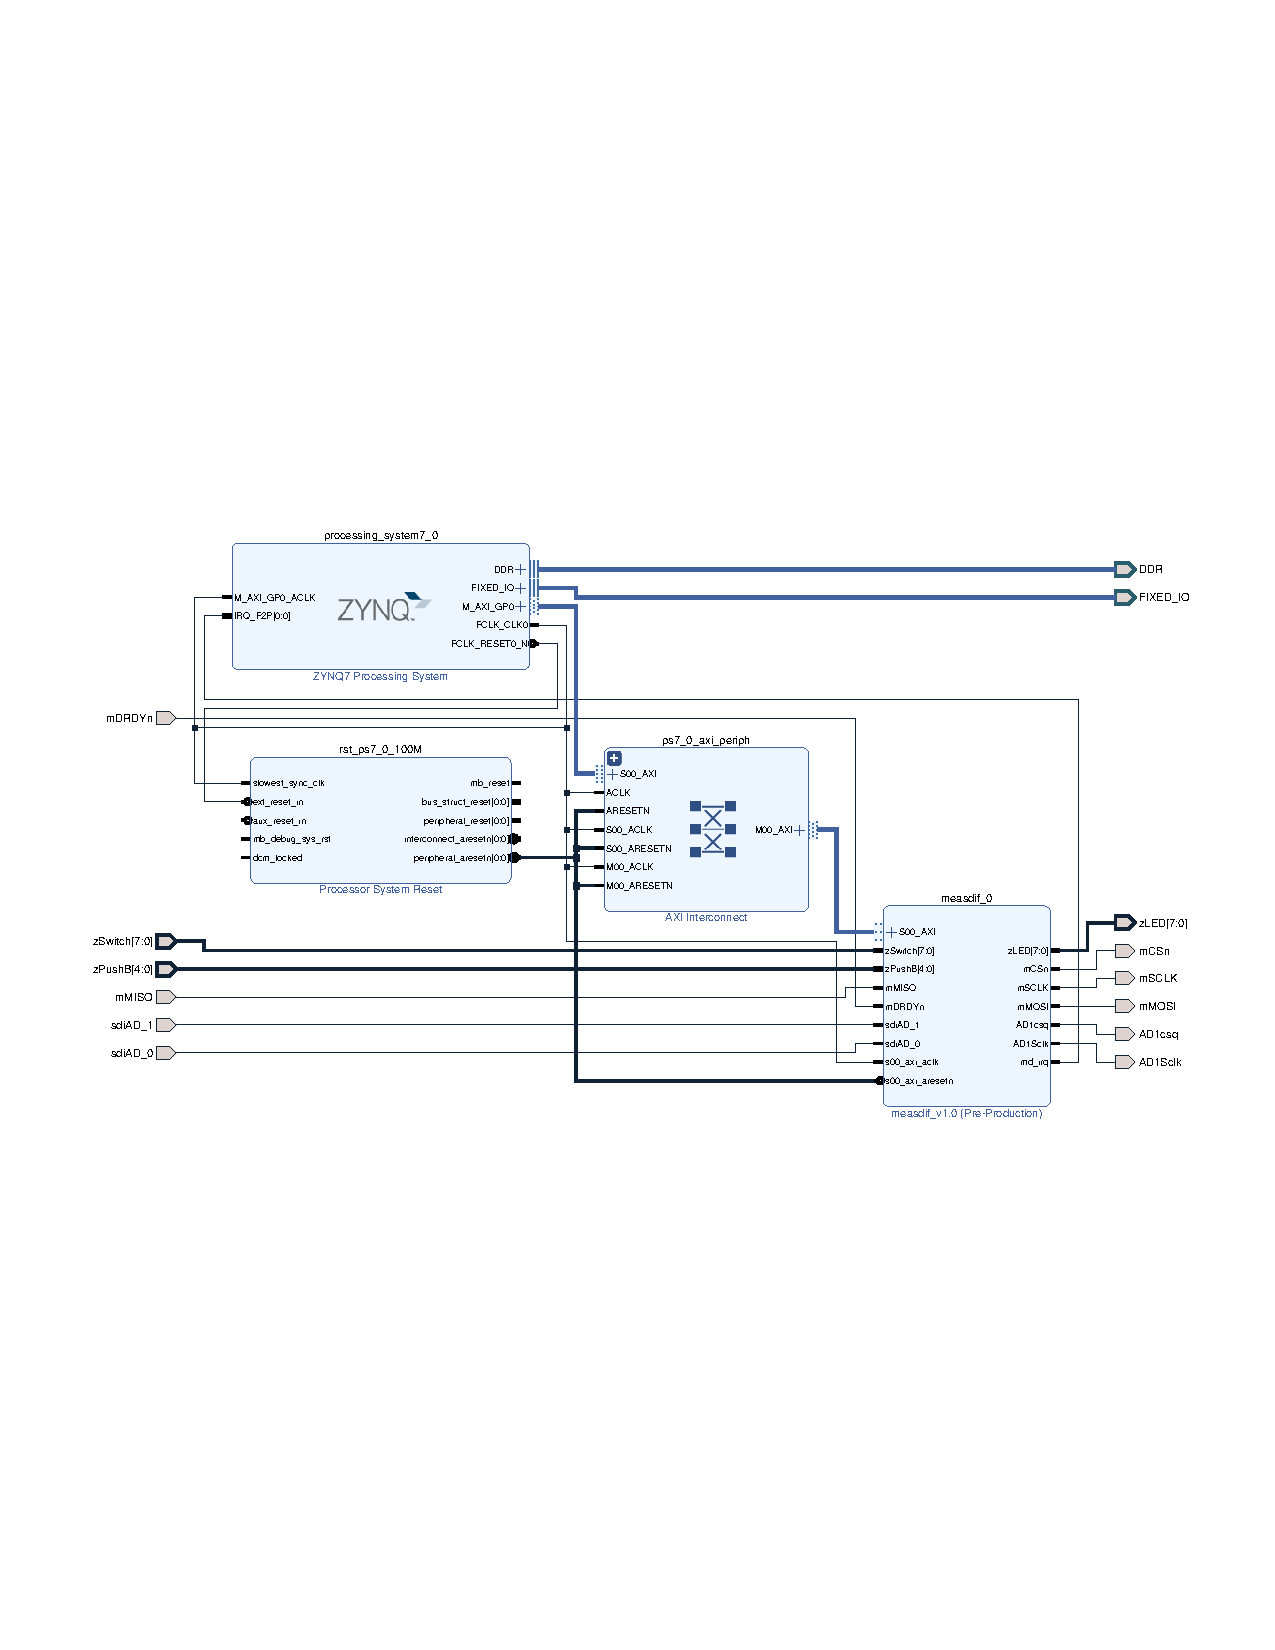
\includegraphics[width = \textwidth, trim = 1.5cm 8cm 1.5cm 8cm, clip]{media/zedbmg_sys.pdf}
\caption{Block Diagram of the whole system in Vivado}
\end{center}
\end{figure} 

After making the block diagram inside Vivado, the design has to be synthesized and for the synthesis first a constraint file for the board has to be written. The constraint file (.xdc file) define the hardware on the board such as Switches and Push Buttons which are used for this project. It specifies which pins to be used for which input and output. Since we are using the Zedboard FPGA developing board we need to write the constraint file for this board. \\
The following code shows the complete contraint file used for this project. 
\begin{minted}[breaklines, tabsize = 4, bgcolor = lightgray, numbers = left]{tcl}
############################
# On-board leds            #
############################
# all 8 leds
set_property PACKAGE_PIN T22 [get_ports zLED[0]]
set_property PACKAGE_PIN T21 [get_ports zLED[1]]
set_property PACKAGE_PIN U22 [get_ports zLED[2]]
set_property PACKAGE_PIN U21 [get_ports zLED[3]]
set_property PACKAGE_PIN V22 [get_ports zLED[4]]
set_property PACKAGE_PIN W22 [get_ports zLED[5]]
set_property PACKAGE_PIN U19 [get_ports zLED[6]]
set_property PACKAGE_PIN U14 [get_ports zLED[7]]
set_property IOSTANDARD LVCMOS33 [get_ports zLED]

# zSwitch [7:0]
############################
# On-board switches        #
############################
set_property PACKAGE_PIN F22 [get_ports zSwitch[0]]
set_property PACKAGE_PIN G22 [get_ports zSwitch[1]]
set_property PACKAGE_PIN H22 [get_ports zSwitch[2]]
set_property PACKAGE_PIN F21 [get_ports zSwitch[3]]
set_property PACKAGE_PIN H19 [get_ports zSwitch[4]]
set_property PACKAGE_PIN H18 [get_ports zSwitch[5]]
set_property PACKAGE_PIN H17 [get_ports zSwitch[6]]
set_property PACKAGE_PIN M15 [get_ports zSwitch[7]]
set_property IOSTANDARD LVCMOS18 [get_ports zSwitch]

# zPushB [4:0]
############################
# On-board pushbuttons     #
############################
set_property PACKAGE_PIN P16 [get_ports zPushB[0]]
set_property PACKAGE_PIN R16 [get_ports zPushB[1]]
set_property PACKAGE_PIN N15 [get_ports zPushB[2]]
set_property PACKAGE_PIN R18 [get_ports zPushB[3]]
set_property PACKAGE_PIN T18 [get_ports zPushB[4]]
set_property IOSTANDARD LVCMOS18 [get_ports zPushB]


# PMOD JA
############################
# PmodAD1                 #
############################
#NET JA1         LOC = Y11   | IOSTANDARD=LVCMOS33;
#NET JA2         LOC = AA11  | IOSTANDARD=LVCMOS33;
#NET JA3         LOC = Y10   | IOSTANDARD=LVCMOS33;
#NET JA4         LOC = AA9   | IOSTANDARD=LVCMOS33;
set_property PACKAGE_PIN Y11 [get_ports AD1csq]
set_property IOSTANDARD LVCMOS33 [get_ports AD1csq]
set_property PACKAGE_PIN AA9 [get_ports AD1Sclk]
set_property IOSTANDARD LVCMOS33 [get_ports AD1Sclk]
set_property PACKAGE_PIN Y10 [get_ports sdiAD_1]
set_property IOSTANDARD LVCMOS33 [get_ports sdiAD_1]
set_property PACKAGE_PIN AA11 [get_ports sdiAD_0]
set_property IOSTANDARD LVCMOS33 [get_ports sdiAD_0]


# PMOD JC1
############################
# MAXPMB1#                 #
############################
#NET JC1_N         LOC = AB6  | IOSTANDARD=LVCMOS33;  # "JC1_N" - 2
#NET JC1_P         LOC = AB7  | IOSTANDARD=LVCMOS33;  # "JC1_P" - 1
#NET JC2_N         LOC = AA4  | IOSTANDARD=LVCMOS33;  # "JC2_N" - 4
#NET JC2_P         LOC = Y4   | IOSTANDARD=LVCMOS33;  # "JC2_P" - 3
#NET JC3_N         LOC = T6   | IOSTANDARD=LVCMOS33;  # "JC3_N" - 8
#NET JC3_P         LOC = R6   | IOSTANDARD=LVCMOS33;  # "JC3_P" - 7
#NET JC4_N         LOC = U4   | IOSTANDARD=LVCMOS33;  # "JC4_N" -10
#NET JC4_P         LOC = T4   | IOSTANDARD=LVCMOS33;  # "JC4_P" - 9
set_property PACKAGE_PIN AB7 [get_ports mCSn]
set_property IOSTANDARD LVCMOS33 [get_ports mCSn]
set_property PACKAGE_PIN AB6 [get_ports mMOSI]
set_property IOSTANDARD LVCMOS33 [get_ports mMOSI]
set_property PACKAGE_PIN Y4 [get_ports mMISO]
set_property IOSTANDARD LVCMOS33 [get_ports mMISO]
set_property PACKAGE_PIN AA4 [get_ports mSCLK]
set_property IOSTANDARD LVCMOS33 [get_ports mSCLK]
set_property PACKAGE_PIN R6 [get_ports mDRDYn]
set_property IOSTANDARD LVCMOS33 [get_ports mDRDYn]

\end{minted}

After adding the constraint file, the design, and HDL wrapper is generated for the whole design, since the block diagram design is not synthesizable. After HDL wrapper is generated the design is synthesized inside Vivado and after synthesization, the bitstream is generated for the design. \\
After generation of the bistream, the generated hardware should be exported in .xsa format to use it for software development either in Bare Metal Programming or Embedded Linux Programming. 





\newpage
\null 
\vfill
\begin{center}
\textbf{\large Haizon Helet Cruz (42708)}
\end{center}
\vfill
\fancyhead[L]{Introduction to Embedded Linux Development (Petalinux) (Haizon Helet Cruz 42708)}
\newpage

\chapter{Introduction to Embedded Linux Development (Petalinux)}
\section{Building Embedded Linux (Petalinux)}

This section describes the complete procedure followed to integrate the Vivado hardware design with the PetaLinux environment and enable communication between the AXI-based measurement IP and the user-space C application. The main objective of this section was to create a Linux-based software platform capable of accessing AXI registers implemented in programmable logic and exposing them to a C application via a character device inteface.

\section{Hardware Import Process}
We are working with Zynq-7000 (ZedBoard) and custom PL IP blocks (ADC inteface, switches, buttons. Hardware created in Vivado and exported as the .xsa file. The first step involved in this procedure is to create a petalinux project using the following command:
\begin{minted}[tabsize=4, breaklines, bgcolor=lightgray]{text}
petalinux-create --type project --template zynq --name meas_gateway
\end{minted}

This command helps create a project using petalinux more specifically it helps in generating a yocto-based Linux build environment which is configured to Zynq architecture. This will create the kernel, rootfs, and boot configuration directories which can be edited according to a project’s specification and prepares cross-compilation infrastructure for ARM Cortex-A9.

Once the creation process is completed, use the command:
\begin{minted}[tabsize=4, breaklines, bgcolor=lightgray]{text}
 petalinux-config –get-hw-description =file_path 
\end{minted}

The hardware import petalinux auto-generates: 
\begin{itemize}
\item system-top.dts
\item pl.dtsi
\item Kernel configuration fragments
\end{itemize}
These AXI files must be verified to ensure that:
\begin{itemize}
    \item The AXI base address matches Vivado address editor
    \item The interrupt ID matches the GIC configuration
    \item The address range aligns with the IP register map
\end{itemize}

After configuration, the system can be built using:
\begin{minted}[tabsize=4, breaklines, bgcolor=lightgray]{text}
petalinux-build
\end{minted}













This step helps in extracting AXI Peripheral base addresses, Interrupt routing, memory regions and building the project using \texttt{petalinux-build} command generates \texttt{system-top.dts,  pl.dtsi}, Kernel configuration fragments. This step ensures Linux kernel is aware of the AXI measurement IP, the physical base address assigned in Vivado matches what Linux expects, Interrupt numbers align with the GIC configuration. This step is very important, without which the kernel would boot but the measurement IP would not exist from Linux’s perspective.


\subsection{Device Tree Entry}
The device tree serves as a critical data structure used by the bootloader and operating system to describe the non-discoverable hardware components of a system. In embedded environments, such as those utilizing Xilinx AXI-based architectures, the kernel cannot automatically proble for every peripheral’s memory location or interrupt line. To resolve this, the DT provides a hierarchical map in a format called a Device Tree Source (.dts).
After hardware import, the generated device tree should be inspected and checked if it is correct. 

The device tree format is as follows: 
\begin{minted}[tabsize=4, breaklines, bgcolor=lightgray]{text}
    measdif_0: measdif@43c00000 {
        clock-names = "s00_axi_aclk";
        clocks = <&clkc 15>;
        compatible = "xlnx,measdif-1.0";
        interrupt-names = "md_irq";
        interrupt-parent = <&intc>;
        interrupts = <0 29 4>;
        reg = <0x43c00000 0x10000>;
        xlnx,s00-axi-addr-width = <0x5>;
        xlnx,s00-axi-data-width = <0x20>;
    };
\end{minted}

This entry defines the following details:
\begin{itemize}
    \item Base address: 0x43c00000
    \item Address range: 0x10000
    \item Interrupt ID: 29
    \item Compatible string for driver matching which is "xlnx,measdif-1.0". This is the "ID card" for the hardware. The Linux kernel uses this string to search for a matching driver.
\end{itemize}

This node is essential for platform driver binding.


\section{Linux Kernel Module}
The \texttt{meascdd.c} module serves as a bridge between the physical hardware registers of the PMB1\# board and the Linux operating system. By registering as a character device driver, it creates a filesystem entry at \texttt{/dev/meascdd}, allowing user-space programs to interact with hardware as if they were readiing or writing to a standard file. This abstraction is critical because user-space applications are prohibited from accessing physical memory addresses directly for security and stability reasons; the driver handles these “preiviliged” operations on their behalf.

The module is specifically structured as a platform driver, a choice dictated by the nature of the hardware. Unlike a USB or a PCIe device, which can be “queried” by the system to identify themselves, AXI-based hardware components in an FPGA or SoC are non-discoverable. The kernel relies on a Device tree to provide the physical address and interrupt lines for the device. When the kernel finds a “compatible” string in the device tree that matches the driver’s name, it triggers the meascdd\_probe function to initialize the hardware.

Inside the \texttt{meascdd\_probe} function, the driver performs essential memory management through I/O remapping. It takes the physical memory address range defined in the Device Tree and maps it into the kernel's virtual address space using ioremap. 
The physical base address retrieved using \texttt{platform\_get\_resource()} is mapped into kernel virtual address using \texttt{ioremap(physical\_address, size)}, 

This allows the driver to use functions like \texttt{ioread32} and \texttt{iowrite32} to manipulate hardware registers safely. Additionally, the probe function requests a major number for the device and creates a device class, which automates the creation of the \texttt{/dev/meascdd} node.

Data exchange between the user application and the hardware is managed through the \texttt{dev\_read} and \texttt{dev\_write} functions using a custom structure called \texttt{MeasObj\_struct}. When the user calls \texttt{write()}, the driver uses copy\_from\_user to pull data into kernel space, then determines which hardware register to update based on the rnum field. Conversely, dev\_read uses copy\_to\_user to send register values back to the application. This structured communication ensures that both the user program and the kernel agree on the format of the data being swapped.

The driver enforces a fixed-size communication structure; 
\begin{minted}[tabsize=4, breaklines, bgcolor=lightgray]{c}
    typedef struct {
        unsigned int rnum;
        unsigned int rvalue;
    } MeasObj_struct;
\end{minted}

Before processing data the driver verifies if len is equal to \texttt{MEASOBJ\_SIZE}. This guarantees data integrity and prevents malformed user-space requests.


Finally, the driver handles asynchronous events through an Interrupt Service Routine (ISR) named meascdd\_irq. When the hardware signals an event (like a timer expiration), the kernel pauses current tasks to run this routine. The ISR in this module performs a specific sequence: it acknowledges the interrupt to the hardware, toggles a bit in the Led\_Output variable to blink an LED, and then re-enables the interrupt for the next cycle. This allows the system to respond to real-time hardware events without the user-space program having to constantly "poll" or check the status of the device.

\section{Memory-Mapped I/O and Register Addressing}
The driver implements a strict 32-bit word-aligned addressing scheme to communicate with the AXI-based hardware. While user-space applications refer to registers by simple integer indices (0 through 7), the kernel module must translate these into physical memory offsets. This is achieved by taking the base address acquired during the platform device probe and adding an offset calculated as the register number multiplied by 4 (Base+4×n).

This specific addressing logic ensures that every ioread32 and iowrite32 call aligns perfectly with the AXI interconnect's expectations. By abstracting the physical memory map (e.g., 0x43C00000) into a simple virtual index for the user-space program, the driver prevents manual addressing errors that could lead to system crashes or bus errors.

\begin{figure}[H]
    \centering
    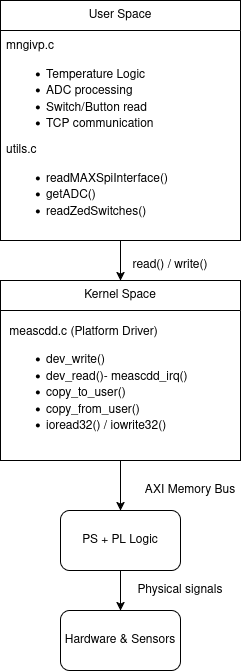
\includegraphics[width=0.25\textwidth]{media/h2peta1.png}
    \caption{Complete Architecture Diagram}
    \label{fig:meascddArch}
\end{figure}


\subsubsection{Stateful Communication via REGNUM\_ID}
A unique architectural feature of this system is the use of a "control ID" to manage the state of the communication channel. The driver uses a reserved constant, \texttt{REGNUM\_ID (0x0FF)}, to distinguish between a command to write data to the hardware and a command to select a register for future observation.

When the user-space program writes a \texttt{MeasObj\_struct} with rnum set to \texttt{0x0FF}, the driver does not toggle any hardware pins; instead, it updates an internal kernel variable named \texttt{Reg\_Num}. This variable then dictates which hardware register will be accessed during the subsequent read() system call. This design allows the user-space program to "poll" different hardware registers (such as status vs. data registers) using a single, unified file descriptor.

\subsection{Critical Section Management and LED Bitmasking}
The driver manages a shared hardware resource: the LED and status register (Register 0). In this system, Register 0 is modified by two different entities: the user-space application (to set status LEDs) and the Kernel's Interrupt Service Routine (to toggle a "heartbeat" LED).

To prevent these two entities from overwriting each other, the dev\_write function employs bitmasking logic. When a user writes to Register 0, the driver preserves the 7th bit (the interrupt-controlled LED) while updating the lower 7 bits with user data. This ensures that the visual "heartbeat" maintained by the meascdd\_irq routine remains consistent even when the user application is actively changing the state of other LEDs.

\subsection{Interrupt Service Routine and Timing}
The hardware is designed to generate periodic interrupts based on a 100ms timer. The driver defines this timing constant as 0x009896ff. Upon receiving an interrupt signal, the \texttt{meascdd\_irq} routine is executed by the kernel.
The ISR follows a precise "Acknowledge and Re-arm" sequence:
\begin{itemize}
\item Acknowledgment: It writes the MBINT\_ACKN flag to the control register to clear the hardware interrupt line.
\item Action: It toggles the 7th bit of the Led\_Output variable using a XOR operation \texttt{(\^\ = 0x080)} to create the blinking effect.
\item Re-arming: It writes back the MBINT\_ENABLE flag along with the timer constant to ensure the next interrupt occurs in exactly 100ms.
\end{itemize}

\subsection{Application Integration: Temperature Sensing Logic}
The system's primary utility is demonstrated in the TempMeasure function, which interfaces with a MAX31865 RTD-to-Digital converter. The user-space program uses the driver to "bit-bang" configuration data into the device.
For example, the application sends the hex value 0x81 to initialize the PMB1 hardware and 0xA1 to trigger a single-shot temperature conversion. The driver facilitates this by wrapping these hex commands into MeasObj\_struct objects, which are then transmitted across the kernel boundary to the physical SPI-over-AXI bridge. The application then calculates the final temperature using the formula T=xadc×0.03125−256.0, where xadc is the raw data retrieved via the driver from registers 1 and 2.

\subsection{Driver Registration and Probe Execution}
The seamless integration fo the meascdd module into the Linux kernel is governed by the Platform Driver framework, which automates hardware discovery through the device tree. Rather than manually searching for hardware, the kernel uses a matching mechanism to link the driver code to the physical AXI IP core defined in the system’s firmware. 

\begin{minted}[tabsize=4, breaklines, bgcolor=lightgray]{c}
static struct platform_driver meascdd_driver = {
    .probe = meascdd_probe,
    .remove = meascdd_remove,
    .driver = {
    .name = "meascdd",
    .of_match_table = meascdd_of_match,
    },
};
\end{minted}

The \texttt{platform\_driver} structure formally registers the \texttt{meascdd} driver with the Linux kernel’s platform driver framework. This structure defines the lifecycle callbacks and matching configuration required for driver binding.

Key elements:
\begin{itemize}
    \item \texttt{.probe}: Points to \texttt{meascdd\_probe()}, which is executed when the kernel finds a matching device tree node
    \item \texttt{.remove}: Points to \texttt{meascdd\_remove()}, which is called when the driver is unloaded or the device is removed.
    \item \texttt{.name}: Logical driver name used internally by the kernel.
    \item \texttt{.of\_match\_table}: Links the driver to the Open Firmware matching table (\texttt{meascdd\_of\_match}). This enables automatic binding when the kernel parses a Device Tree node containing: “xlnx, measdif-1.0” compatible string.
\end{itemize}

During kernel boot or module insertion, the Device Tree Blob (DTB) is parsed. When a node with \texttt{compatible = "xlnx,measdif-1.0"} is detected, the platform driver framework invokes \texttt{meascdd\_probe()}.



\subsubsection{Device Tree parsing and probe execution}
During the kernel's boot or module insertion phase, the system parses the Device Tree Blob (DTB) to identify available hardware. The kernel specifically looks for a node containing the property compatible = "xlnx,measdif-1.0". This string acts as a unique hardware identifier. The meascdd.c module contains an of\_match\_table that explicitly lists this string, signaling to the kernel that this specific driver is capable of managing that hardware instance.

\subsubsection{The Probe Sequence}
Once a match is confirmed, the kernel triggers the meascdd\_probe function, which serves as the "constructor" for the device. This function is responsible for several critical setup tasks:
\begin{itemize}
\item Resource discovery: The driver calls platform\_get\_resource to retrieve the physical base address and the Interrupt Request (IRQ) number assigned to the hardware in the Device Tree.
\item Memory locking: It invokes request\_mem\_region to ensure no other driver can claim the physical memory space assigned to the PMB1 registers.
\item I/O Mapping: The physical address is converted into a kernel-accessible virtual address via ioremap, which is then stored in the global Meas\_Base\_Address pointer for use by the read and write functions.
\end{itemize}

\subsubsection{Character Device Creation}
Beyond hardware initialization, the probe function establishes the user-space interface. It dynamically allocates a major number using register\_chrdev and creates a device class in sysfs. This sequence culminates in the creation of the /dev/meascdd node, effectively bridging the gap between the kernel's internal hardware representation and the standard Linux filesystem.


\subsubsection{Interrupt Attachment}
The final stage of the probe execution involves the request\_irq function. The driver registers the meascdd\_irq routine as the handler for the device's hardware interrupt. By doing so, the driver tells the kernel exactly which code to execute whenever the hardware timer—defined by the TIMER100ms constant—reaches its terminal count. This registration allows the driver to toggle the LED "heartbeat" without requiring any active processing from the user-space application.

\section{System execution Sequence diagram}
\subsection{Boot and Driver Binding}
\begin{figure}[H]
    \centering
    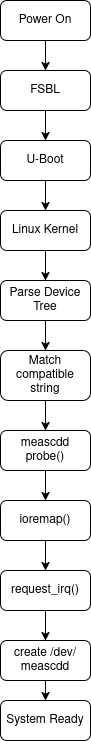
\includegraphics[scale = 0.7]{media/h2peta2.png}
    \caption{Boot and Driver Binding Architecture}
    \label{fig:bootAndDriverBinding}
\end{figure}

\subsection{Register write transition}
This architecture diagram demonstrates the sequence of starting ADC.

\begin{figure}[H]
    \centering
    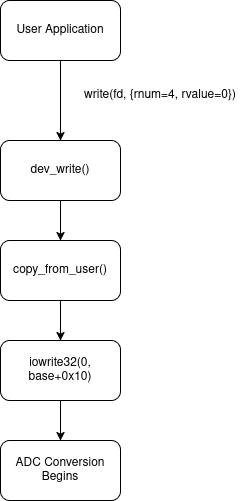
\includegraphics[scale = 0.6]{media/h2peta3.png}
    \caption{Register write transition Architecture}
    \label{fig:registerWriteTransition}
\end{figure}

\subsection{Register read transition}
\begin{figure}[H]
    \centering
    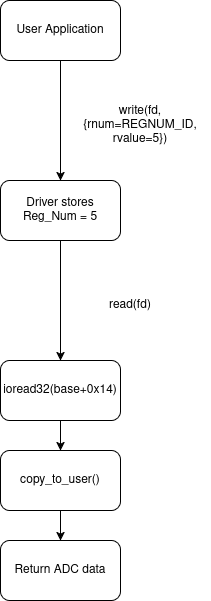
\includegraphics[scale = 0.6]{media/h2peta4.png}
    \caption{Register read transition Architecture}
    \label{fig:registerReadTransition}
\end{figure}


\subsection{Building the Image}
After integrating the custom kernel module (meascdd.c) and user-space application (mngivp.c) are integrated into the project environment, the next step is building the system image. 

The image is built using the petalinux command 
\begin{minted}[tabsize=4, breaklines, bgcolor=lightgray]{text}
petalinux-build
\end{minted}

Unlike compiling a standalone C program, this command invokes the Yocto-based build system to generate an entire bootable Linux software stack tailored for the target Zynq-7000 platform.

\subsubsection{PetaLinux Build Stages}
Each stage of image build process is given below
\begin{itemize}
\item Kernel compilation (inlcuding LKM)
\item Device Tree configuration
\item RootFS generation
\item FIT image packaging
\end{itemize}




\subsubsection{Component Integration}
The final output of this process is typically the image.ub file, which is a FIT (Flattened Image Tree) format. This single file acts as a container for several critical components:

\begin{itemize}
\item \textbf{The Kernel Image:} The core operating system that manages system resources and schedules tasks.
\item \textbf{The Root Filesystem (RootFS)}: The environment where the mngivp application resides and where the character device node is created.
\item \textbf{The Device Tree Blob (DTB)}: The binary map that tells the driver exactly where the PMB1 hardware registers are located in memory.
\end{itemize}

\subsubsection{Deployment and Integration}
Once the build is complete, the image.ub and the bootloader (BOOT.BIN) are copied to the SD card. Upon power-up:
\begin{itemize}
\item The kernel parses the device tree and matches the "compatible" string to the meascdd driver.
\item The probe function executes, remapping the hardware registers and registering the major number.
\item The user executes ./mngivp, which opens /dev/meascdd to begin temperature or ADC acquisition.
\end{itemize}

\subsubsection{Verification of the Build}
A successful build can be verified by checking the /lib/modules/ directory on the target rootfs for the meascdd.ko file or by running ls /dev/meascdd once the system has booted. If the build was successful, the hardware heartbeat LED managed by meascdd\_irq should begin toggling at 100ms intervals as soon as the driver is loaded.

\subsection{Runtime Verification}
The final step involved is to verify that the integration performed during the build process correctly translates into functional hardware-software communication on the physical board.
After booting the board, the following were verified:
\begin{itemize}
\item Driver loaded: This command lists all currently loaded kernel modules. Seeing meascdd in this list confirms that the kernel successfully matched the "compatible" string from the Device Tree with the driver's of\_match\_table and executed the module's initialization code.
\item Device node exists: The presence of this file confirms that the major number was successfully registered and that the meascdd\_probe function completed its character device registration sequence without error.
\item dmesg logs: This allows for the inspection of specific printk and dev\_info messages generated during the driver's execution.
\end{itemize}
Based on the logs and system state, the following critical milestones were reached:
\begin{itemize}
\item AXI Base Address Mapped: The log confirms that platform\_get\_resource successfully retrieved the physical memory address from the Device Tree and that ioremap successfully mapped it to a kernel-accessible virtual address (stored in Meas\_Base\_Address).
\item Interrupt Registered: The verification confirms that request\_irq was successful for the IRQ number specified in the Device Tree. This is often visually confirmed by the 100ms LED "heartbeat" toggled by the meascdd\_irq routine.
\item Device Successfully Initialized: The "MEAScdd: registered correctly" and "MEAScdd: initialized" messages confirm that the major number was allocated and the platform driver is ready to handle read() and write() calls from the mngivp.c application.
\end{itemize}


\subsection{Summary}
The PetaLinux integration establishes a complete hardware–software abstraction layer between the AXI-based measurement IP and the user-space application. The Vivado hardware design is exported as an XSA file and imported into PetaLinux, enabling automatic generation of the device tree and kernel configuration aligned with the Zynq-7000 architecture.

The custom meascdd driver is implemented as a Linux platform driver and bound to the hardware instance using Open Firmware device tree matching. Upon successful compatible string matching, the kernel invokes the \texttt{probe()} function, which performs resource discovery, physical memory mapping using \texttt{ioremap()}, interrupt registration via \texttt{request\_irq()}, and character device creation.

User-space communication is achieved through a structured interface (\texttt{MeasObj\_struct}) using \texttt{copy\_from\_user()} and \texttt{copy\_to\_user()} mechanisms. Register addressing follows a strict 32-bit word-aligned mapping scheme to ensure AXI compliance. A stateful register selection mechanism using \texttt{REGNUM\_ID} enables efficient multi-register access over a single character device interface.

Periodic hardware interrupts are handled by the \texttt{meascdd\_irq} ISR, which acknowledges the interrupt, updates system state, and re-arms the timer to maintain deterministic 100 ms execution cycles.

The complete system image is generated using the Yocto-based PetaLinux build system, producing a bootable FIT image (\texttt{image.ub}) containing the Linux kernel, device tree, and root filesystem. Runtime verification confirms correct driver binding, memory mapping, interrupt servicing, and character device initialization.
This architecture ensures secure, structured, and deterministic communication between FPGA-based AXI hardware and high-level user applications within a Linux environment.







% =====================================================================================
\newpage
\null 
\vfill
\begin{center}
The Application built by:\\ 
\textbf{\large Mohammad Mahdi Mohammadi (42719)\\
Mohamamd Reza Rahimi (42756)\\ 
Akshay Vastrad (42723)}
\end{center}
\vfill
\thispagestyle{empty}
\clearpage


\newpage
\null 
\vfill
\begin{center}
	\textbf{\large Mohammad Reza Rahimi (42756) } \\ 
\end{center}
\vfill
\fancyhead[L]{Ring Buffer Development (Mohammad Reza Rahimi 42756)}
\newpage

\chapter{Ring Buffer Development}



\section{Ring Buffer Fundamentals}\label{ring-buffer-fundamentals}
This section introduces the basic concepts of ring buffers (also known
as circular buffers) and explains why they are widely used in embedded
and real-time systems. In the context of the Measurement Network
Gateway, the ring buffer is the central data structure that enables
real-time streaming of sensor data to a remote client. Ring buffers are
widely used in embedded and real-time systems because they provide
predictable time behaviour and fixed memory usage.

\subsection{Definition and Concept}\label{definition-and-concept}

A ring buffer or we can say circular buffer, is a fixed-size data
structure that stores elements in first‑in, first‑out (FIFO) order. It
is implemented as a statically allocated array together with one or more
indices that move through the array in a circular fashion.

New elements are written at a write pointer (also called the head).
Elements are removed at a read pointer (also called the tail). It wrap
round to index zero when a pointer reaches the end of array, so the
storage structure is like ring rather than a linear block memory.

This wrap around behavior cause the data can be added continuously
without moving or reallocating memory. when the buffer is full, the new
elements will inserting either block or overwriting the oldest elements,
it depends on the chosen policy.

\begin{figure}[H]
\centering 
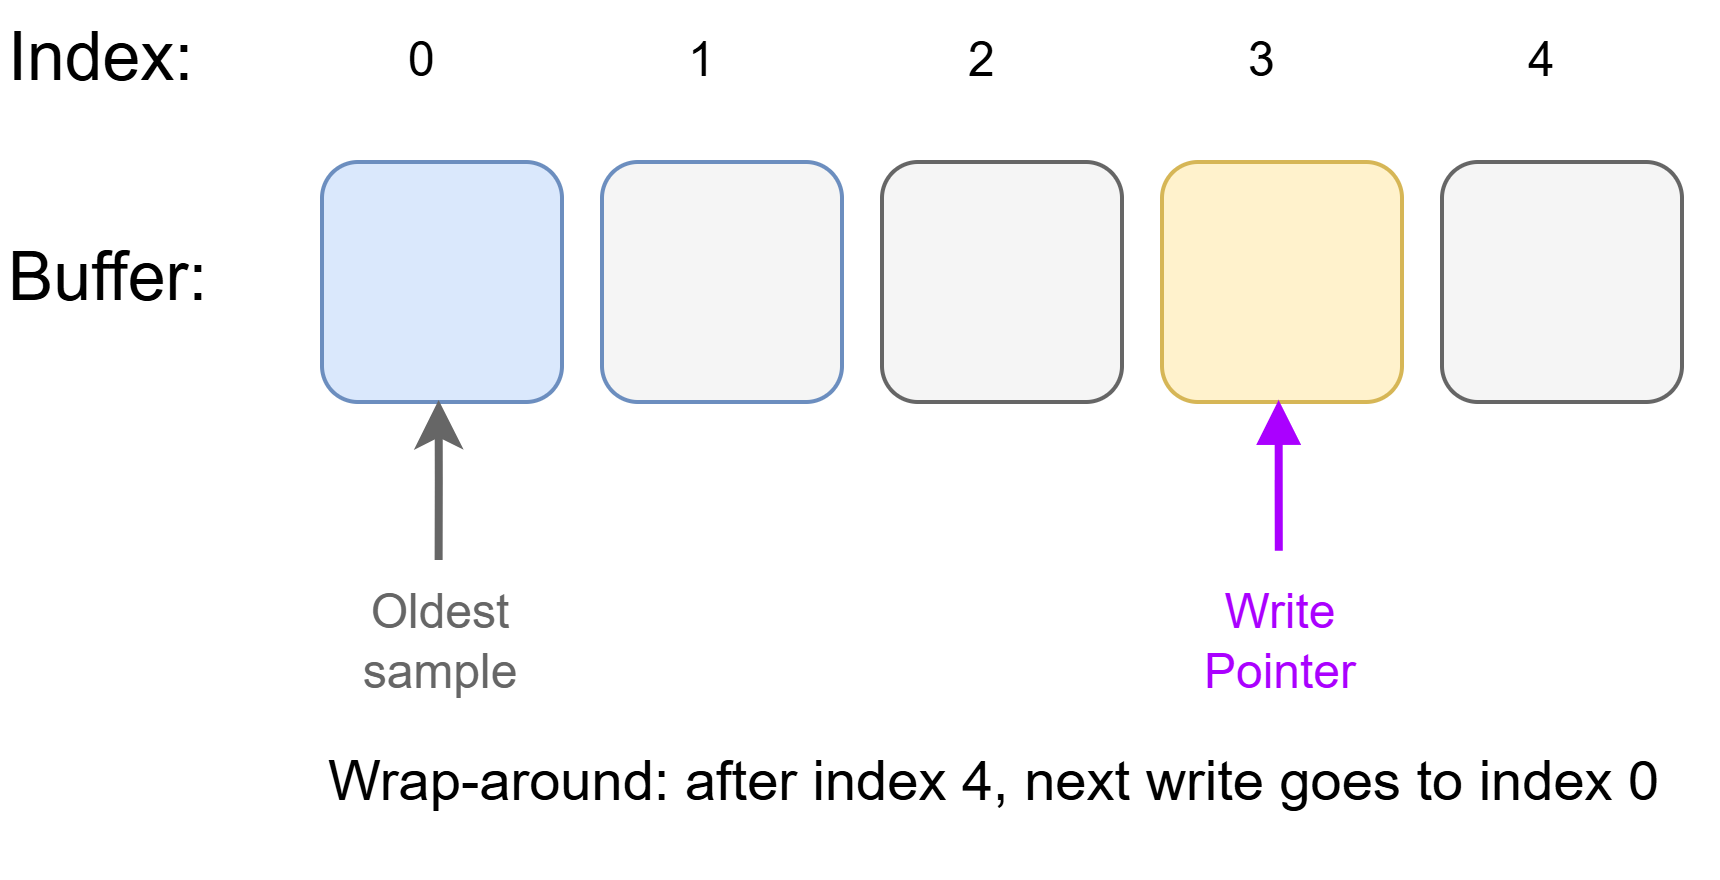
\includegraphics[width=0.7\textwidth]{media/image1.png}
\caption{Illustration of a circular buffer with capacity 5}
\end{figure}

\subsection{Operational
Characteristics}\label{operational-characteristics}

There are two primary operation that ring buffer supports, which are
inserting a new element (push) and removing the oldest element (pop).
The push is going to write data at the current write pointer and then
advances this pointer, but the pop operation different which reads data
from the current read position and advances the read pointer. In the
constant time \(O(1)\), both operation will execute, which is
independent of buffer size, because no data needs to be shifted in
memory.

The buffer has a fixed capacity, defined at compile time. With inserting
elements the number of stored elements will increase till the buffer
going to become full. Once it becomes full the implementation apply the
policy, either block further writes until space becomes available or
overwrite the oldest stored elements as new data arrives. To choose
either block the ring buffer or overwrite is depending on the
requirements of the application, especially with respect to data loss
and real-time constraints.

\subsection{Use Cases in Embedded and Real-Time
Systems}\label{use-cases-in-embedded-and-real-time-systems}

Ring buffers are widely used in embedded and real-time systems because
they provide predictable time behaviour and fixed memory usage. Typical
applications include UART receive buffers, sensor data acquisition
buffers, audio sample queues, and logging mechanisms, where continuous
streams of data must be stored temporarily without dynamic memory
allocation.

In producer--consumer scenarios, such as interrupt-driven input feeding
a slower processing task, the ring buffer decouples the producer and
consumer rates. The producer can store new data as soon as it becomes
available, while the consumer processes data whenever CPU time and
system load permit. This decoupling reduces the risk of data loss due to
short-term timing variations and simplifies the design of real-time data
pipelines.

\section{Ring Buffer in the Measurement Network
Gateway}\label{ring-buffer-in-the-measurement-network-gateway}

This section describes how the ring buffer is used inside the
Measurement Network Gateway. It first explains the functional
requirements and role of the buffer, then presents the concrete data
structure~RingB\_Struct, and finally discusses the timer and
timestamping mechanism that is tightly coupled to the buffer design.

\subsection{2.1 Requirements and Role}\label{requirements-and-role}

In the Measurement Network Gateway, two main threads handle sensor data:

\begin{itemize}
\item
  A~sensor thread~that periodically reads physical sensors (temperature,
  ADC channels, switches, push buttons) and produces timestamped
  samples.
\item
  A~server thread~that packages these samples into TCP payloads and
  transmits them to a remote client.
\end{itemize}

These threads have different timing characteristics. The sensor thread
must respect precise sampling intervals, while the server thread is
constrained by network latency, client behaviour, and the TCP stack. To
decouple these two activities, the gateway requires an intermediate
storage mechanism that:

\begin{itemize}
\item
  Preserves the temporal order of measurements (FIFO behaviour).
\item
  Allows the sensor thread to continue sampling even when the network is
  temporarily slow or unavailable.
\item
  Uses fixed memory to avoid dynamic allocation in an embedded
  environment.
\item
  Supports concurrent access from two threads in a safe manner.
\end{itemize}

The ring buffer serves as a bounded FIFO queue between the sensor thread
(producer) and the server thread(consumer). After the acquisition the
new sample are push to the ring buffer by the sensor thread and the
server thread will pop those samples from rig buffer whenever it is
ready to send data to the client. This design ensures that the sampling
logic is independent of network timing and that the gateway can handle
short bursts of data without losing the most recent measurements.

In this project's implementation, once the buffer is full, new data
overwrites the oldest stored samples. This policy will explain in
details in the next section.

\begin{figure}[H]
\centering 
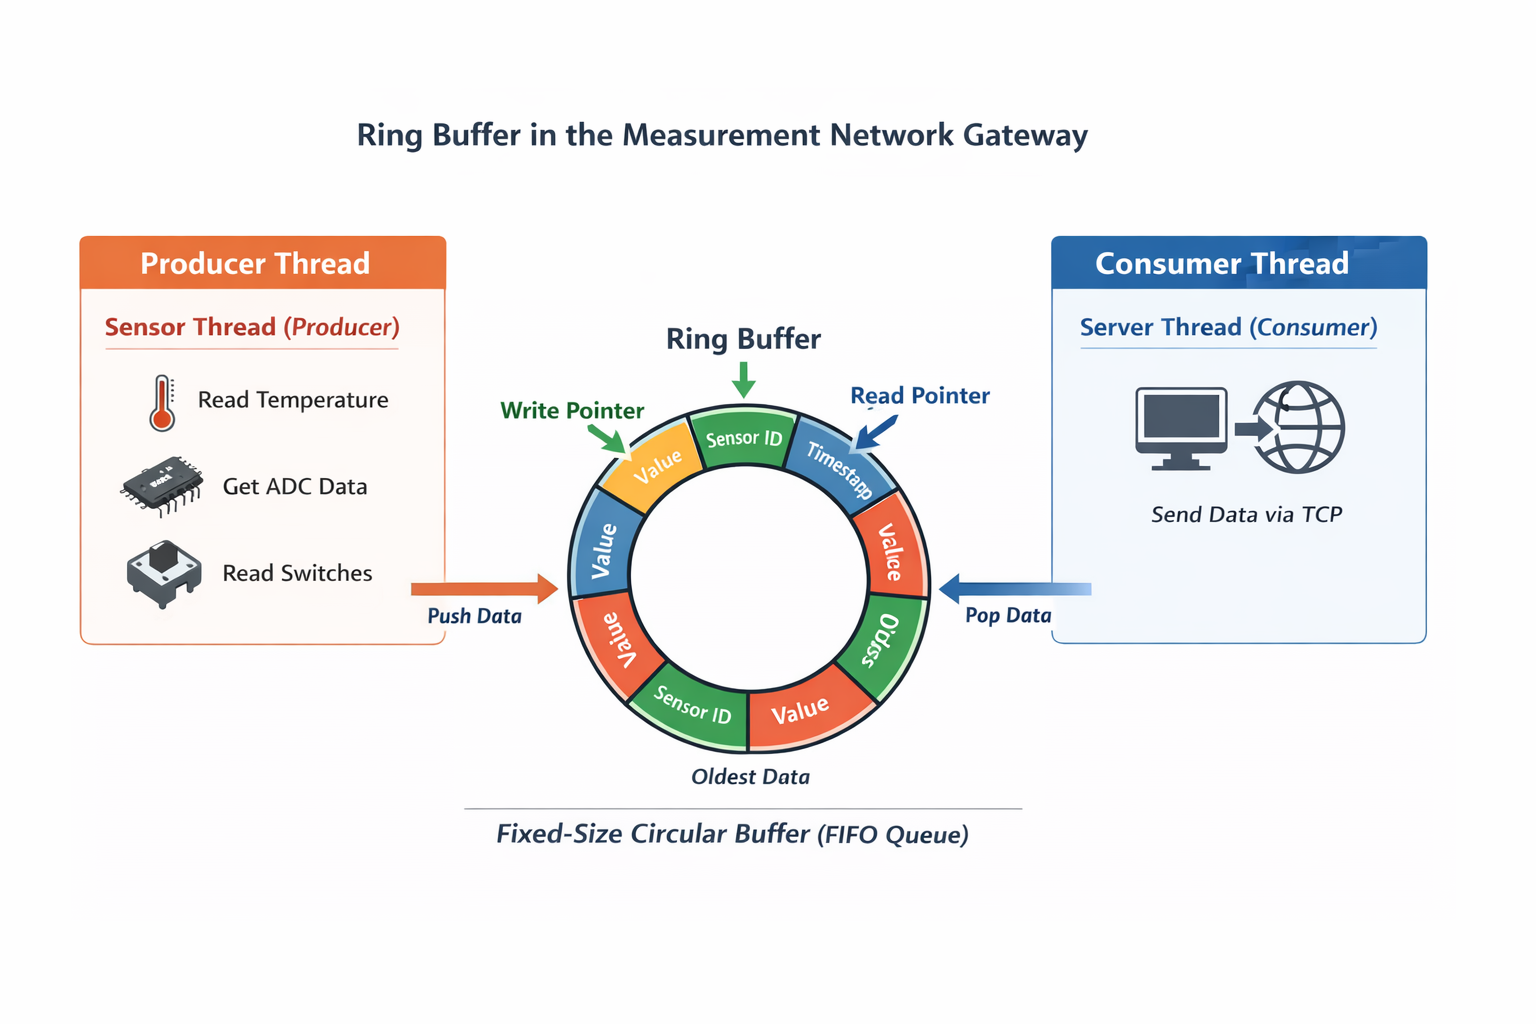
\includegraphics[width = 0.9\textwidth]{media/image2.png}
\caption{Producer–consumer use of the ring buffer.}
\end{figure}

\subsection{Data Structure \texttt{RingB\_Strcut}}
The ring buffer is implemented as a global instance of the structure \texttt{RingB\_Struct}, defined in \texttt{Ring\_Buffer.h}. It groups all storage arrays and control variables needed for FIFO measurement buffering.

\begin{minted}[bgcolor = lightgray, tabsize = 4, breaklines]{c}
#define RBUF_LEN 2048

typedef struct {
    pthread_mutex_t bmutex;              // mutex for thread safety
    volatile int      sensor_id[RBUF_LEN];
    volatile uint64_t tstamp[RBUF_LEN];
    volatile int      svalue[RBUF_LEN];
    volatile int      rb_pointer;        // write index
    volatile int      rb_cnt;            // number of valid entries
} RingB_Struct;

extern RingB_Struct Ring_Buf;
\end{minted}

The fields have the following roles:
\begin{itemize}
\item \texttt{RBUF\_LEN} defines the fixed capacity of the buffer in number of samples (2048 in this project).
\item bmutex protects all accesses to the buffer so that the sensor and server threads cannot modify it at the same time.
\item \texttt{sensor\_id[]}, \texttt{tstamp[]}, and \texttt{svalue[]} are parallel arrays; for any index i, the triple \texttt{(sensor\_id[i], tstamp[i], svalue[i])} represents one complete measurement sample.
\item \texttt{rb\_pointer} points to the position where the next pushed sample will be stored. It is advanced with wrap-around after each write.
\item \texttt{rb\_cnt} stores how many valid samples are currently buffered. It is going to increase on push but decrease on pop. The buffer is full when the \texttt{rb\_cnt} reaches \texttt{RBUF\_LEN} and new samples will overwrite the oldest one while \texttt{rb\_cnt} stays constant.
\end{itemize}
With the storing of the write pointer and a count, the implementation can reconstruct the index of the oldest sample on demand, without the read pointer separated.  This way keeps the state small and also this way will support full FIFO behavior.

\subsection{Timer and Timestamping}
Each measurement in the ring buffer is tagged with a timestamp in microseconds relative to the gateway's startup time. This is implemented in Ring\_Buffer.c using a monotonic system clock.
At startup, the sensor thread calls \texttt{InitTimer()} once to record a reference time:

\begin{minted}[bgcolor = lightgray, tabsize = 4, breaklines]{c}
static uint64_t US_startup_time;

void InitTimer(void)
{
    struct timespec ts;
    clock_gettime(CLOCK_MONOTONIC, &ts);
    US_startup_time = ts.tv_sec * 1000000ULL + ts.tv_nsec / 1000ULL;
}
\end{minted}

Whenever a sensor value is acquired, the thread calls \texttt{GetElapsedTime()} to obtain the current timestamp:

\begin{minted}[bgcolor = lightgray, tabsize = 4, breaklines]{c}
static uint64_t US_startup_time;

void InitTimer(void)
{
    struct timespec ts;
    clock_gettime(CLOCK_MONOTONIC, &ts);
    US_startup_time = ts.tv_sec * 1000000ULL + ts.tv_nsec / 1000ULL;
}
\end{minted}

In this way:
\begin{itemize}
\item InitTimer records a fixed reference time US\_startup\_time in microseconds, using CLOCK\_MONOTONIC, which is not affected by wall clock changes.
\item GetElapsedTime returns the elapsed time since startup, also in microseconds.
\item The sensor thread passes this value as the timestamp parameter of \texttt{PushRB}, so each ring buffer entry contains a time stamp consistent across all sensors.
\end{itemize}
This scheme allows the client to reconstruct the exact timing of measurements and to align data from different sensors on a common time axis.

\section{Implementation Details}
This section explains how the ring buffer is brought into a defined initial state and how measurements are inserted and removed. It covers the initialization functions \texttt{InitTimer} and \texttt{InitRingBuffer}, followed by the \texttt{PushRB} and \texttt{PopRB} operations that implement the FIFO behaviour.

\subsection{Initialization (\texttt{InitTimer}, \texttt{InitRingBuffer})}
The initialization phase prepares both the time base for timestamps and the ring buffer storage. \texttt{InitTimer} was introduced in Section 2.3; it records the startup time using the monotonic system clock and is called once by the sensor thread.

The function \texttt{InitRingBuffer} brings the buffer into a defined empty state:
\begin{minted}[bgcolor = lightgray, tabsize = 4, breaklines]{c}
void InitRingBuffer(void)
{
    pthread_mutex_init(&Ring_Buf.bmutex, NULL);

    Ring_Buf.rb_pointer = 0;
    Ring_Buf.rb_cnt     = 0;

    for (int i = 0; i < RBUF_LEN; i++) {
        Ring_Buf.sensor_id[i] = 0;
        Ring_Buf.svalue[i]    = 0;
        Ring_Buf.tstamp[i]    = 0;
    }
}
\end{minted}
This performs three steps:
\begin{itemize}
\item Initializes the mutex bmutex, enabling safe concurrent access from the sensor and server threads.
\item Sets \texttt{rb\_pointer = 0} and \texttt{rb\_cnt = 0}, marking the buffer as empty and indicating that the first write will occur at index 0.
\item Clears all entries in \texttt{sensor\_id}, \texttt{svalue}, and \texttt{tstamp} to a known state, which simplifies debugging and guarantees deterministic start up behaviour.
\end{itemize}
After \texttt{InitTimer} and \texttt{InitRingBuffer} have been called, the gateway has a clean time reference and an empty, ready to use ring buffer.


\subsection{Push Operation (\texttt{PushRB})}
The function \texttt{PushRB} inserts a new measurement sample into the ring buffer. It is called by the sensor thread whenever a sensor value is acquired.

\begin{minted}[bgcolor = lightgray, tabsize = 4, breaklines]{c}
void PushRB(int sid, uint64_t ts, int sv)
{
    pthread_mutex_lock(&Ring_Buf.bmutex);

    Ring_Buf.sensor_id[Ring_Buf.rb_pointer] = sid;
    Ring_Buf.tstamp[Ring_Buf.rb_pointer]    = ts;
    Ring_Buf.svalue[Ring_Buf.rb_pointer]    = sv;

    if (Ring_Buf.rb_cnt < RBUF_LEN) {
        Ring_Buf.rb_cnt++;
    }

    Ring_Buf.rb_pointer = (Ring_Buf.rb_pointer + 1) % RBUF_LEN;

    pthread_mutex_unlock(&Ring_Buf.bmutex);
}
\end{minted}
The behaviour is as follows:
\begin{itemize}
\item The mutex bmutex is locked to ensure exclusive access to the buffer state during the update.
\item The triple (sid, ts, sv) is written at index \texttt{rb\_pointer}, forming one complete measurement sample.
\item If the buffer is not yet full \texttt{(rb\_cnt < RBUF\_LEN)}, the count of valid entries is incremented; otherwise it remains at \texttt{RBUF\_LEN}, and the oldest sample will later be overwritten.
\item The write pointer \texttt{rb\_pointer} is advanced and wrapped around using modulo arithmetic, implementing the circular structure.
\item Finally, the mutex is unlocked so that other threads can access the buffer again.
\end{itemize}
Conceptually, each call to \texttt{PushRB} appends one new sample to the logical end of the FIFO queue. When the producer is faster than the consumer and the buffer becomes full, new pushes overwrite the oldest data while always preserving the most recent measurements.

\subsection{Pop Operation \texttt{PopRB}}
The \texttt{PopRB} function removes the oldest available sample from the ring buffer and returns it to the caller. It is typically used by the server thread when it prepares a data packet to send to the client.

\begin{minted}[bgcolor = lightgray, tabsize = 4, breaklines]{c}
int PopRB(int *sid, uint64_t *ts, int *sv)
{
    pthread_mutex_lock(&Ring_Buf.bmutex);

    if (Ring_Buf.rb_cnt == 0) {
        pthread_mutex_unlock(&Ring_Buf.bmutex);
        return -1;                      // buffer empty
    }

    int idx = (Ring_Buf.rb_pointer - Ring_Buf.rb_cnt + RBUF_LEN) % RBUF_LEN;

    *sid = Ring_Buf.sensor_id[idx];
    *ts  = Ring_Buf.tstamp[idx];
    *sv  = Ring_Buf.svalue[idx];
    Ring_Buf.rb_cnt--;

    pthread_mutex_unlock(&Ring_Buf.bmutex);
    return 0;                           // success
}
\end{minted}

The steps are:
\begin{itemize}
	\item The mutex is locked to protect the shared state.
	\item If \texttt{rb\_cnt} is zero, the buffer is empty, the mutex is unlocked and -1 is returned to signal “no data available”.
	\item Otherwise, the index of the oldest sample is computed as
\texttt{idx = (rb\_pointer-rb\_cnt+RBUF\_LEN) mod RBUF\_LEN}
which moves \texttt{rb\_cnt} positions back from the next write position, with wrap around.
	\item The sensor ID, timestamp, and value at index idx are copied into the caller’s output parameters, and rb\_cnt is decremented to reflect that one entry has been removed.
	\item Finally, the mutex is unlocked and the function returns 0 to indicate success.
\end{itemize}

\textbf{Example}: Computing the Oldest Sample Index. 
To illustrate the index calculation:
\begin{center}
\texttt{idx = (rb\_pointer-rb\_cnt+RBUF\_LEN) mod RBUF\_LEN}
\end{center}
consider a small ring buffer with \texttt{RBUF\_LEN = 5}. Assume the following state:
Given the following ring buffer state:
\begin{itemize}
    \item $\texttt{RBUF\_LEN} = 5$
    \item $\texttt{rb\_pointer} = 2$ (next write will go to index 2)
    \item $\texttt{rb\_cnt} = 3$ (three valid samples stored)
\end{itemize}

The last three writes have filled three positions immediately before
\texttt{rb\_pointer} in the circular sense. The valid entries are therefore
at indices:
\begin{itemize}
    \item index 4 \quad (oldest sample)
    \item index 0
    \item index 1 \quad (newest sample)
\end{itemize}

The \texttt{PopRB} function must locate the oldest sample, which is at index~4.
Using the formula:
\[
    \texttt{idx} = (\texttt{rb\_pointer} - \texttt{rb\_cnt} + \texttt{RBUF\_LEN})
                  \;\%\; \texttt{RBUF\_LEN}
                = (2 - 3 + 5) \;\%\; 5 = 4
\]

So $\texttt{idx} = 4$, exactly the index of the oldest stored entry. After
\texttt{PopRB} reads the sample at index~4 and decrements \texttt{rb\_cnt}
to 2, the remaining valid samples are at indices~0 and~1, and a subsequent
call with the updated state will correctly return index~0 as the next oldest
entry.

\section{Runtime Data Flow and System Architecture}
This chapter describes the runtime behavior of the Measurement Network Gateway and explains how measurement data flows through the system from hardware acquisition to remote visualization. Rather than focusing on individual hardware devices or data structures in isolation, this chapter presents a system-level view of how threads, timing, and buffering interact during operation.

\subsection{	Thread Architecture Overview}
The Measurement Network Gateway is built around a small multithreaded architecture that separates sensor acquisition from network communication. Two main threads are used in conjunction with a shared ring buffer to transport measurement data to a remote client.

The sensor thread is responsible for interacting with the hardware. It periodically samples physical sensors, generates timestamps, and inserts measurement records into the ring buffer. This thread acts as the producer of measurement data and operates independently of network conditions or client behavior.

The server thread functions as the consumer. It retrieves measurement entries from the ring buffer and transmits them to a remote GUI or client application using a TCP connection. By decoupling the server thread from direct hardware access, the system ensures that temporary network delays do not directly interfere with sensor sampling.

At a high level, the runtime data path through the system is:

\begin{figure}[H]
\centering 
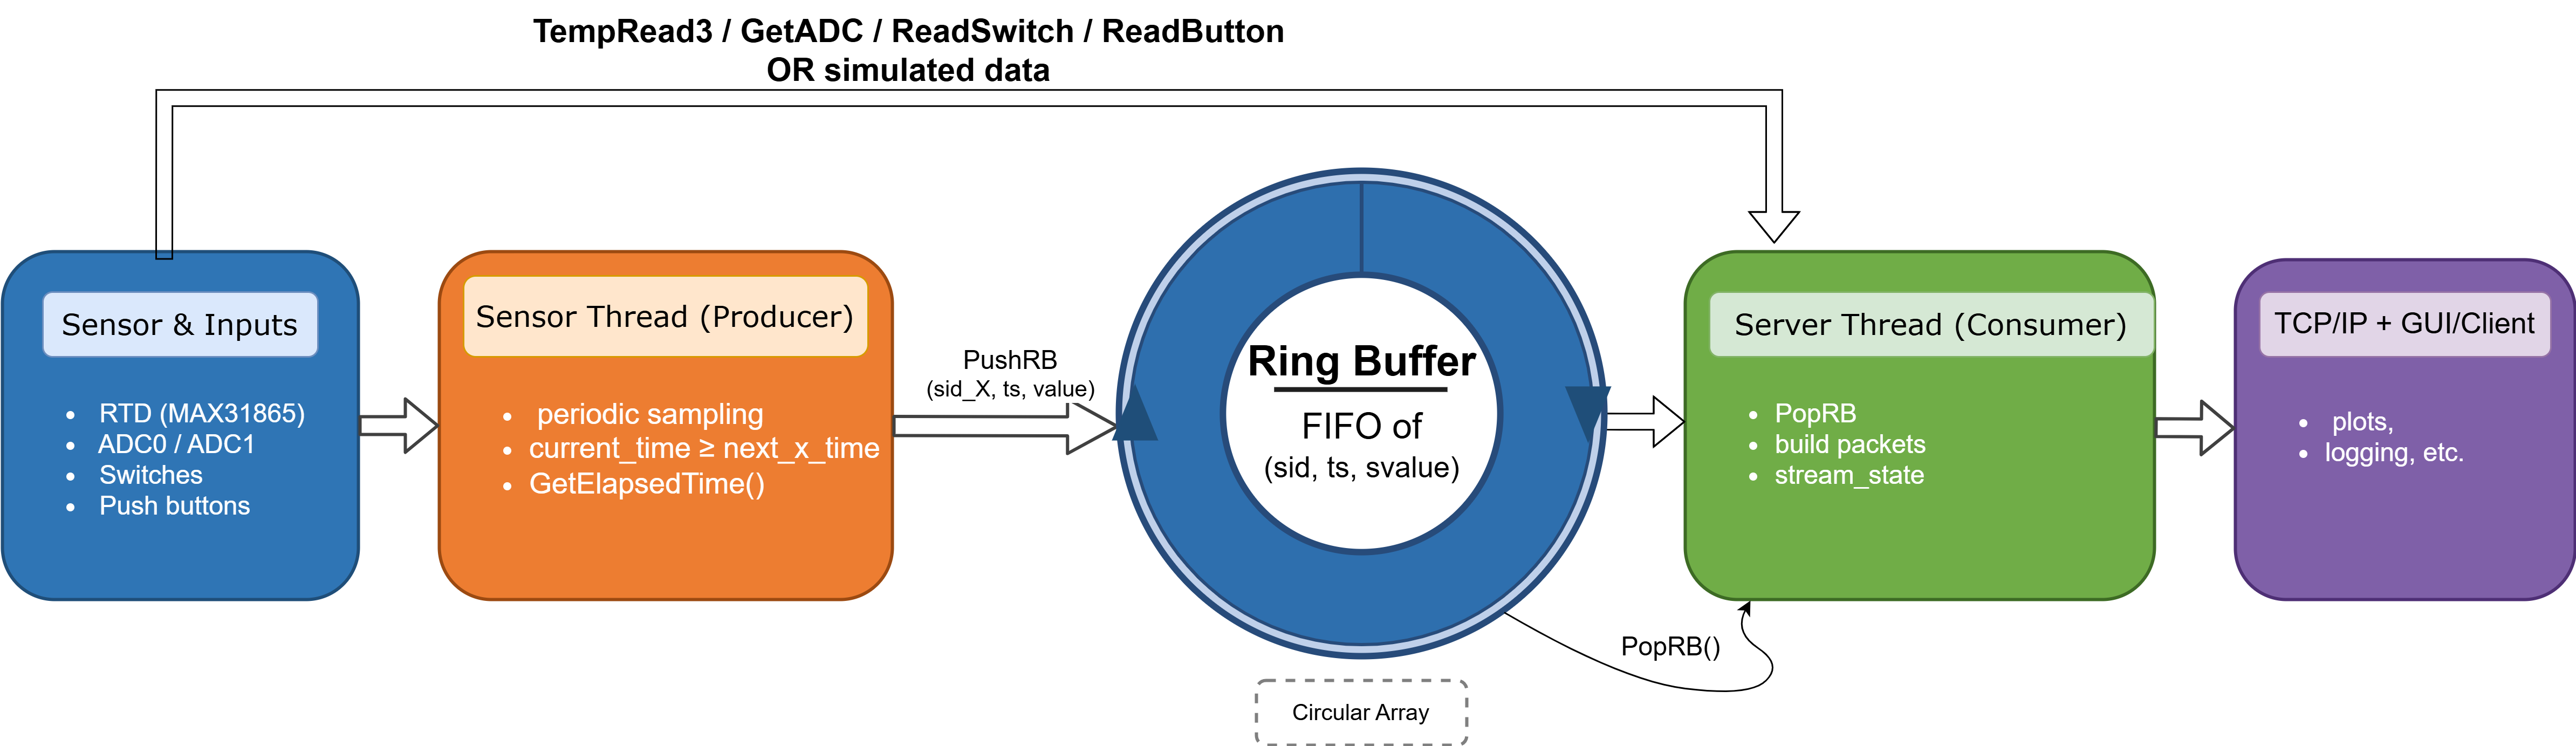
\includegraphics[width = \textwidth]{media/image3.png}
\caption{Runtime data flow of the Measurement Network Gateway}
\end{figure}
This architecture provides a clear separation of concerns and allows each subsystem to operate at its own pace.

\subsection{Producer-Consumer Model}
The ring buffer is acting like a bridge between the sensor thread and the server thread which follows  a classical producer–consumer model implemented. Sensor thread read data or measure the samples and then inserts them into ring buffer, while server thread consumes those samples and sends to the client. 

On the producer side, sensor is sampled each time and then the result is written into the ring buffer using the unified insertion function:

\begin{minted}[bgcolor = lightgray, tabsize = 4, breaklines]{c}
PushRB(sid_temp, current_time, temp_data);
PushRB(sid_adc0, current_time, adc0_data);
PushRB(sid_switches, current_time, switches_data);
\end{minted}

The \texttt{PushRB()} function encapsulates the ring buffer write operation. Internally, it writes a structured entry containing the sensor identifier, timestamp, and value into the current head position and advances the head index. If the buffer is already full, the oldest entry is overwritten by advancing the tail index according to the overwrite policy.

A simplified conceptual form of the write operation is:

\begin{minted}[bgcolor = lightgray, tabsize = 4, breaklines]{c}
rbuf[head].sensor_id = sid;
rbuf[head].tstamp    = timestamp;
rbuf[head].svalue    = value;

head = (head + 1) % RBUF_LEN;

if (head == tail) {
    tail = (tail + 1) % RBUF_LEN;   // overwrite oldest
}
\end{minted}
On the consumer side, the server thread retrieves entries from the ring buffer before sending them over TCP. The read operation removes the oldest available entry and advances the tail index:

\begin{minted}[bgcolor = lightgray, tabsize = 4, breaklines]{c}
if (PopRB(&entry) == 0) {
    send(client_socket, &entry, sizeof(entry), 0);
}
\end{minted}

Here, \texttt{PopRB()} copies the oldest buffered measurement into a local structure and updates the tail pointer. If the buffer is empty, no data is transmitted during that iteration.
Because both threads access shared indices and buffer memory, appropriate synchronization mechanisms are used to ensure consistency. The ring buffer therefore acts as a controlled exchange boundary between acquisition and communication subsystems.

This design allows the producer and consumer to operate asynchronously. The sensor thread maintains deterministic sampling timing, while the server thread operates according to network conditions. The ring buffer absorbs short-term rate mismatches and enforces the overwrite-on-full policy described later. 

\subsection{Timing and Scheduling Strategy}
Sensor sampling is controlled by time based scheduling mechanism which implemented within sensor thread. With initialization, a reference timer is started \texttt{InitTimer}, and elapsed time is subsequently obtained using \texttt{GetElapsedTime}. All timestamps are in microseconds related to system startup. 

The sensor thread maintains an independent next sampling deadline for the each sensor channel. While execution time, the current elapsed time is compared against each channel’s scheduled sampling time using conditions of the form \texttt{current\_time >= next\_x\_time}. If the condition is met, the sensor is sampled and the result is pushed into the ring buffer.

With this procedure, each sensor operate its own sampling frequency while sharing a single execution thread. Microsecond-resolution timestamps enable precise sampling and minimize jitter, particularly when multiple sensors operate at different rates. The timestamp method is much more better than blocking delays which maintains predictable timing behavior and efficient CPU utilization.


\section{Per-Sensor Mapping into the Ring Buffer}
This chapter describes how each physical hardware channel is represented inside the ring buffer. While previous chapters explained the hardware interfaces and the buffer mechanism independently, this section connects the two perspectives. It answers a central architectural question: how does each real-world signal appear as a structured entry in the shared ring buffer?

\subsection{	Sensor ID Enumeration}
To distinguish between different hardware sources within a unified buffer structure, each sensor channel is assigned a unique identifier using the following enumeration:

\begin{minted}[bgcolor = lightgray, tabsize = 4, breaklines]{c}
typedef enum
{
    sid_temp     = 1,
    sid_adc0     = 2,
    sid_adc1     = 3,
    sid_switches = 4,
    sid_pushb    = 5
} sensor_id;
\end{minted}
The \texttt{sensor\_id} value is stored in every ring buffer entry and encodes the origin of the measurement. Because the ring buffer stores heterogeneous data from multiple hardware channels in a single FIFO structure, this identifier is essential for interpreting the stored value correctly.

The consumer side, also server thread and the GUI are using the \texttt{sid} field to interpret the corresponding \texttt{svalue} . Based on the sensor ID the value can be a raw ADC count, a scaled temperature value, or a digital bitfield. This method can keep ring buffer on uniform way while still preserving the semantic meaning of each hardware signal.

\begin{figure}[H]
\centering 
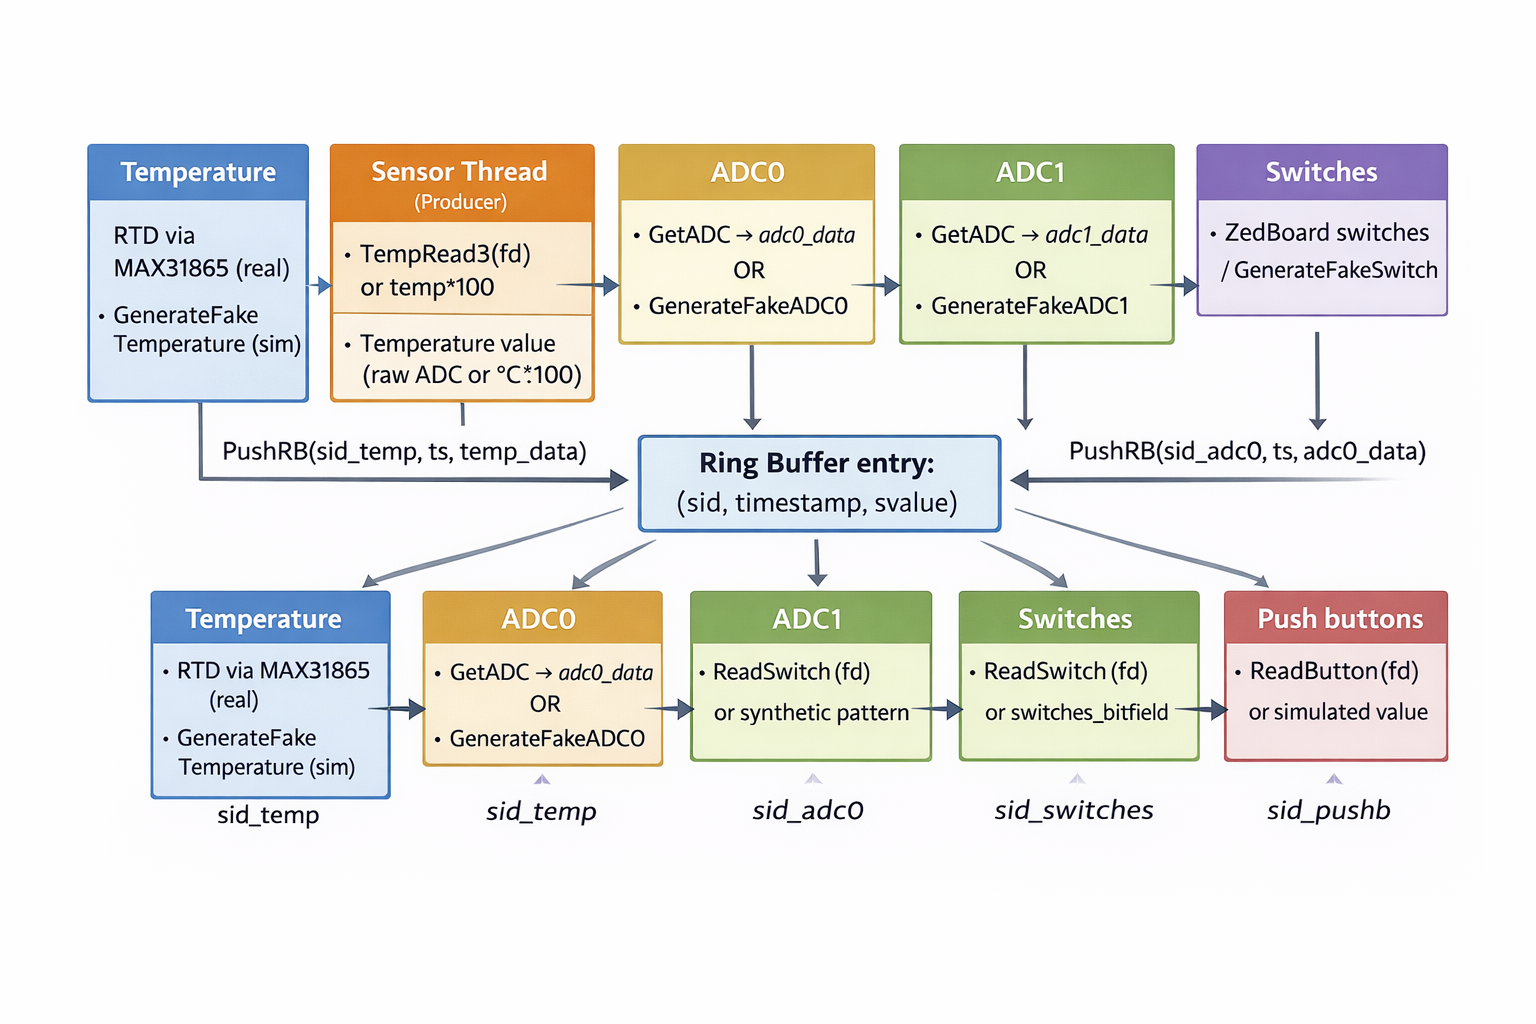
\includegraphics[width = 0.8\textwidth, trim = 0cm 2cm 0cm 0cm, clip]{media/image4.png}
\caption{Per sensor mapping into the ring buffer}
\label{fig-image4}
\end{figure}

The mapping between sensor IDs and hardware sources is summarized below:
\begin{table}[h]
    \centering
    \begin{tabular}{|c|l|l|l|}
        \hline
        \textbf{SID Value} & \textbf{Enum Name} & \textbf{Hardware Source} & \textbf{Typical Units} \\
        \hline
        1 & \texttt{sid\_temp}     & MAX31865 RTD input      & raw ADC code / \textdegree C \\
        2 & \texttt{sid\_adc0}     & ADC channel 0           & raw ADC counts \\
        3 & \texttt{sid\_adc1}     & ADC channel 1           & raw ADC counts \\
        4 & \texttt{sid\_switches} & ZedBoard switches       & 8-bit bitfield \\
        5 & \texttt{sid\_pushb}    & ZedBoard pushbuttons    & 5-bit bitfield \\
        \hline
    \end{tabular}
    \caption{Sensor ID encoding used in the ring buffer}
    \label{tab:sid_values}
\end{table}
This enumeration provides the logical bridge between physical hardware and abstract data records.

\subsection{Temperature Data Path into the Ring Buffer}
The temperature channel follows a time-driven acquisition model within the sensor thread:

\begin{minted}[bgcolor = lightgray, tabsize = 4, breaklines]{c}
if (current_time >= next_temp_time) {
    uint32_t temp_data;
    if (simulation) {
        double temp = GenerateFakeTemperature(current_time);
        temp_data = (uint32_t)(temp * 100);
    } else {
        temp_data = TempRead3(fd);
    }

    PushRB(sid_temp, current_time, temp_data);
    next_temp_time += period_temp_us;
}
\end{minted}
If we look to the hardware side, the temperature measurement is based on the RTD sensor which is connected to the MAX31865 resistance-to-digital converter. The \texttt{TempRead3(fd)} function reads the device via the sensor layer and returns the corresponding ADC value for the RTD resistance. This raw value corresponds directly to the temperature measurement described in the hardware chapter.

In simulation mode, the hardware access is replaced by \texttt{GenerateFakeTemperature()}, which produces a synthetic temperature in degrees Celsius. The value is multiplied by 100 before storage to preserve two decimal places using integer representation.

Regardless of whether the value originates from real hardware or simulation, the final operation is:
\begin{minted}[bgcolor = lightgray, tabsize = 4, breaklines]{c}
PushRB(sid_temp, current_time, temp_data);
\end{minted}
The ring buffer therefore stores a record containing:

\begin{itemize}
\item \texttt{sensor\_id} = sid\_temp
\item \texttt{tstamp} = current\_time (us since startup)
\item \texttt{svalue} = temp\_data (raw ADC or \SI{100}{\degreeCelsius})
\end{itemize}
This unified insertion ensures that downstream components remain independent of the acquisition mode.

\subsection{ADC0 and ADC1 Data Path into the Ring Buffer}
The ADC channels are sampled using similar time-based logic:

\begin{minted}[bgcolor = lightgray, tabsize = 4, breaklines]{c}
PushRB(sid_temp, current_time, temp_data);if (current_time >= next_adc0_time) {
    if (simulation) {
        double dt_adc0 = 1.0 / main_config.adc0_config;
        t_adc0 += dt_adc0;
        adc0_data = (uint32_t)(fake_state.adc0_base
                     + 100.0 * sin(2.0 * PI * freq_adc0 * t_adc0));
    } else {
        GetADC(fd, &adc0_data, &dummy0);
    }
    PushRB(sid_adc0, current_time, adc0_data);
    next_adc0_time += period_adc0_us;
}
\end{minted}
On the hardware side, both \texttt{ADC0} and \texttt{ADC1} are provided by a shared ADC subsystem. The \texttt{GetADC()} function retrieves a combined conversion result from the FPGA/ADC hardware and separates the values corresponding to the two analog channels.

 Although they share physical conversion hardware, they represent distinct electrical input channels.
In simulation mode, synthetic waveforms are generated independently for each channel. ADC0 and ADC1 can therefore exhibit different amplitudes and frequencies, allowing controlled testing of signal behavior.

From the ring buffer perspective, these channels are treated as independent data streams. Each insertion uses either \texttt{sid\_adc0} or \texttt{sid\_adc1}, and each channel maintains its own sampling period and timestamp sequence. Even though they share hardware resources, the ring buffer records them as logically separate measurement streams.

\subsection{Switches and Push Buttons Data Path into the Ring Buffer}
Digital input channels follow the same structural pattern:

\begin{minted}[bgcolor = lightgray, tabsize = 4, breaklines]{c}
if (current_time >= next_switch_time) {
    uint8_t switches_data =
        simulation ? GenerateFakeSwitch(current_time)
                   : ReadSwitch(fd);
    PushRB(sid_switches, current_time, switches_data);
    next_switch_time += period_switch_us;
}

if (current_time >= next_pushb_time) {
    uint8_t pushb_data =
        simulation ? GenerateFakePushButton()
                   : ReadButton(fd);
    PushRB(sid_pushb, current_time, pushb_data);
    next_pushb_time += period_pushb_us;
}
\end{minted}
On the hardware side, \texttt{ReadSwitch()} and \texttt{ReadButton()} access digital input registers in which each bit corresponds to a physical switch or push button on the board. The returned value represents a complete bitfield describing the instantaneous state of all inputs.

In simulation mode, equivalent bit patterns are generated to emulate user interaction.
Within the ring buffer, the entire bitfield is stored as a single integer value using \texttt{sid\_switches} or \texttt{sid\_pushb}. The timestamp attached to each entry allows precise reconstruction of when a switch changed state or when a button was pressed. The GUI decodes the individual bits from the stored value to display the status of each physical input.

\section{Configurable Sampling Rates and Ring Buffer Load}
Each sensor channel’s sampling rate can be changed at runtime using the global configuration and the server side \texttt{configure} command. The configuration parameter such as \texttt{temp\_config, adc0\_config, adc1\_config, switch\_config}, and \texttt{pushb\_config }is going to set the sampling frequency for corresponding sensor in samples per second (Hz).

The frequency is converted to the time period which is shown in microseconds and then the sensor thread use this time to schedule acquisitions:

\begin{minted}[bgcolor = lightgray, tabsize = 4, breaklines]{c}
uint64_t period_temp_us   = (main_config.temp_config > 0) ? 1000000ULL / main_config.temp_config : 0;
uint64_t period_adc0_us   = (main_config.adc0_config > 0) ? 1000000ULL / main_config.adc0_config : 0;
uint64_t period_adc1_us   = (main_config.adc1_config > 0) ? 1000000ULL / main_config.adc1_config : 0;
uint64_t period_switch_us = (main_config.switch_config > 0) ? 1000000ULL / main_config.switch_config : 0;
uint64_t period_pushb_us  = (main_config.pushb_config > 0) ? 1000000ULL / main_config.pushb_config : 0;
\end{minted}
A higher configuration value therefore results in a shorter sampling period and more frequent sensor reads. Each completed sampling event produces one new ring buffer entry via PushRB(). As a result, the total rate at which data is inserted into the ring buffer is equal to the sum of the sampling rates of all enabled sensor channels.

The configuration can be modified dynamically by the client using the configure command, which is parsed and applied by the server thread:

\begin{minted}[bgcolor = lightgray, tabsize = 4, breaklines]{c}
else if (!strncmp(receive_command, "configure ", 10)) {
    config_struct config2;
    sscanf(&receive_command[10], "%u %u %u %u %u",
           &config2.temp_config,
           &config2.adc0_config,
           &config2.adc1_config,
           &config2.switch_config,
           &config2.pushb_config);
    set_config(&config2);
}
\end{minted}

Changing these parameters directly affects the load placed on the ring buffer. Higher sampling frequencies increase the number of samples produced per second and therefore reduce the amount of time the buffer can retain historical data before older entries are overwritten. Conversely, lower sampling rates reduce buffer pressure and increase the effective history depth.

Let me explain with an example, if ADC0 samples at 1000 Hz and the temperature sensor at 100 Hz, the sensor thread will add roughly 1100 samples per second to the ring buffer. With a ring buffer length of 2048 entries, this corresponds to roughly 1.8 seconds of stored history before the overwrite-on-full policy begins to discard the oldest samples, assuming the consumer does not keep up.

This relation of configuration and sampling is connecting directly how the ring buffer is working. Sampling rates are a trade-off between time resolution and buffer lifespan, and should be chosen with consumer throughput and buffer capacity in mind.

\section{Simulation vs. Real Hardware with a Unified Ring Buffer API}
The Measurement Network Gateway supports both real hardware operation and a fully functional simulation mode. During initialization, the application attempts to open the device file \texttt{/dev/meascdd} to access the measurement hardware. If this operation fails, the system automatically enables simulation mode by setting the simulation flag to 1. This allows the application to continue running without physical hardware present.

Within the sensor thread, each sensor acquisition branch checks the value of the simulation flag. In real hardware mode, the system calls the corresponding hardware access functions, such as \texttt{TempRead3(), GetADC(), ReadSwitch(),} and \texttt{ReadButton()}. These functions retrieve actual measurement data from the RTD interface, ADC subsystem, or digital input registers.

In simulation mode, the hardware calls are replaced with synthetic data generators. Functions such as \texttt{GenerateFakeTemperature(), GenerateFakeADC0(), GenerateFakeADC1(),} \texttt{GenerateFakeSwitch()}, and \texttt{GenerateFakePushButton()} produce artificial measurement values that emulate realistic sensor behavior. This enables development, testing, and demonstration without requiring the physical hardware platform.

Despite these different acquisition paths, all sensor branches converge at the same interface:
\begin{minted}[bgcolor = lightgray, tabsize = 4, breaklines]{c}
PushRB(sid_X, current_time, value);
\end{minted}
Whether the value is reading from the real hardware or simulated generator are inserted to the ring buffer by the \texttt{PushRB()} function and the same structured data format. There is no difference for the ring buffer that those data are real data or simulated data. Likewise, the server thread retrieves and transmits measurement records without any knowledge of their origin.

This design ensures that the ring buffer and server components form a hardware-agnostic measurement pipeline. The acquisition layer can switch between real and simulated inputs without changing data transport, buffering, or network streaming. This separating concerns boosts modularity, simplifies testing, and strengthens system reliability.

\section{Design Discussion and Trade-Offs}
The ring buffer implementation in the Measurement Network Gateway reflects several conscious design decisions. This section discusses the most important trade-offs: buffer capacity, overwrite behaviour, and synchronization strategy.

\subsection{Buffer Size and Latency}
The capacity \texttt{RBUF\_LEN} is fixed at 2048 samples. A larger buffer lets the system handle longer delays in the server or network, since more data can be queued before old samples are overwritten. There are also some problem with increasing the ring buffer that consumes more memory and also increase the worst-case latency between acquisition and transmission, which cause the sample should wait much longer in the queue before it is sent.

The chosen size represents a compromise between robustness and responsiveness. For the intended measurement use case, it is more important to have some buffering against short network delays than to guarantee that every historical sample is preserved indefinitely. If strict lossless recording over long periods were required, a different design using larger storage or disk logging would be necessary.

\subsection{Overwrite-on-Full Policy}
When \texttt{rb\_cnt} reaches\texttt{ RBUF\_LEN}, the buffer is logically full. In this implementation, \texttt{PushRB} continues to accept new samples: the write pointer advances and the oldest data is implicitly overwritten, while \texttt{rb\_cnt} remains at \texttt{RBUF\_LEN}. This overwrite-on-full policy prioritises the most recent measurements over older ones.

This choice is appropriate for real-time monitoring, where the client typically cares about the current state of the system and a continuous live stream, rather than a complete historical log. Dropping the oldest samples avoids blocking the sensor thread and preserves real-time behaviour even under temporary overload. The trade-off is that, during prolonged overload, some older measurements are lost. An alternative design would block the producer when the buffer is full, which preserves all data but risks disturbing sampling timings or even stalling the measurement process.

\subsection{Synchronization with a Single Mutex}
With the single \texttt{mutex, bmutex} ensures the safety thread and protect all access to the ring buffer. \texttt{PushRB} and \texttt{PopRB} use the same mutex to protect the small section that updates indices and arrays. This is a very simple and easy approach for a dingle producer and single consumer setup, that works well. The both operation push and pop are short and bounded in time.

You could also use lock-free buffers or separate mutexes and condition variables to indicate data or space availability. This kind of approach will reduce blocking and improve scalability in multi-producer or multi-consumer systems, but there is a drawback which is complexity and difficult to verify it. For this gateway, with one sensor thread and one server thread, a single mutex provides deterministic, constant-time operations without introducing significant overhead.

The ring buffer thus provides a deterministic, bounded, and thread-safe mechanism for exchanging data between the acquisition and networking parts of the gateway. The next chapter builds on this buffering layer to describe the sensor-reading implementation and hardware interface in detail.


















%functions for reading the sensors in MNG (Measurement Network Gateway) 

\section{Sensor Readout Module}
The sensor readout logic of the Measurement Network Gateway is encapsulated in the dedicated source file \texttt{sensor\_read.c} with its public interface declared in \texttt{sensor\_read.h}. This module hides all low level details of SPI communication, ADC configuration, and conversion formulas behind a small set of functions that can be called directly from the sensor thread. In this way, the sensor thread only focuses on sampling timing and pushing values into the ring buffer, while \texttt{sensor\_read.c} provides type safe access to the underlying hardware channels.

The most important functions in this module for physical sensor acquisition are:
\begin{itemize}
    \item MAXWrite and MAXRead for low level SPI access to the MAX31865 RTD converter.
    \item TempRead3 (TempRead) for high level temperature measurement in degrees Celsius.
    \item GetADC for sampling generic analog channels via the on board ADC.
\end{itemize}

The following subsections describe each of these functions in turn and illustrate how they are used inside the application code.


\subsection{MAXWrite: writing to MAX31865 registers}
The function \texttt{MAXWrite} is responsible for sending configuration and control data to the MAX31865 temperature sensor interface over the SPI bus. The MAX31865 is a resistance to digital converter (RTD interface) which measures the resistance of a Pt100/Pt1000 sensor and converts it into a digital code that can later be transformed into a temperature value. To operate correctly, the device must be configured by writing specific bits into its configuration register, for example to select 2 wire/3 wire/4 wire mode, enable bias current, set fault thresholds, or start a one shot conversion.
\texttt{MAXWrite} abstracts this SPI write transaction into a single C function call. Internally, it typically performs the following steps:
\begin{itemize}
    \item Asserts the chip select line (CS) of the MAX31865 to start an SPI frame.
    \item Sends the register address ORed with the write bit as the first byte on the SPI bus.
    \item Sends one or more data bytes that contain the configuration or control information.
    \item De asserts the chip select line to complete the transfer.
\end{itemize}

By concentrating all these operations in MAXWrite, the rest of the code never has to deal with the exact SPI timing or bit level format of the MAX31865 registers; it simply calls MAXWrite with the desired register and data.


\subsection{MAXRead: reading from MAX31865 registers}
Complementary to MAXWrite, the function MAXRead performs SPI read operations from the MAX31865. It is used to obtain the current configuration, read status and fault flags, and, most importantly, fetch the raw RTD measurement data from the converter. The raw measurement is typically stored in two consecutive registers, for example MSB and LSB of the RTD code, which must be read in a single SPI transaction and then combined into a 16 bit value.
Internally, MAXRead carries out these steps:
\begin{itemize}
    \item Asserts the chip select line of the MAX31865.
    \item Sends the start register address ORed with the read bit.
    \item Clocks out one or more bytes from the device while sending dummy bytes on MOSI.
    \item De asserts chip select and returns the received bytes to the caller.
\end{itemize}
This design ensures that every place in the code that needs data from the MAX31865 (for example, the raw RTD code or the fault status) can simply call MAXRead with a register address and buffer, without directly manipulating the SPI peripheral.


\subsection{TempRead: high level temperature acquisition}
The function \texttt{TempRead} provides a complete, high level temperature measurement in degrees Celsius, suitable for direct storage in the ring buffer. From the perspective of the sensor thread, \texttt{TempRead} is the only interface needed to acquire the physical temperature; it hides all the intermediate steps such as triggering a conversion, waiting for completion, reading raw codes, and applying calibration or scaling factors.
A typical measurement cycle performed by TempRead3 involves the following stages:
\begin{itemize}
    \item Optionally configure or re configure the MAX31865 using MAXWrite (for example, clear faults or start a one shot conversion).
    \item Wait for the conversion to complete, either by polling a status bit or using a fixed delay sufficient for the conversion time.
    \item Read the raw RTD code from the MAX31865 using MAXRead as shown above.
    \item Convert the raw code into a resistance value and then into a temperature in degrees Celsius according to the transfer function specified in the datasheet.
    \item Return the resulting floating point temperature value to the caller.
\end{itemize}

Because all these details are encapsulated, the rest of the system can treat TempRead3 as a black box that simply returns the current temperature.


\subsection{GetADC: analog to digital conversion}
In addition to the RTD temperature sensor, the Measurement Network Gateway also acquires analog signals via on board ADC channels. These may be used, for example, to measure external sensor voltages, reference levels, or other analog quantities connected to the system. The function GetADC provides a generic interface to read one sample from a specified ADC channel.

GetADC typically takes an integer channel index as an argument and performs the following steps internally:

\begin{itemize}
    \item Selects the appropriate ADC channel in the ADC peripheral registers.
    \item Starts or triggers a conversion on that channel.
    \item Waits until the conversion is complete (polling a status flag or waiting for an interrupt driven result).
    \item Reads the converted digital sample from the ADC data register.
    \item Returns the sample as an integer (for example a 12 bit or 16 bit value) to the caller.
\end{itemize}
By encapsulating this procedure in GetADC, the sensor thread does not need to know any low level details about ADC configuration or status handling; it simply requests a sample from channel 0 or 1 and receives a ready to use digital value.


\subsection{Integration into the overall measurement path}
Together, \texttt{MAXWrite, MAXRead, TempRead3}, and \texttt{GetADC} form the core of the sensor readout path in the Measurement Network Gateway. All physical measurements flow through these functions before being encoded into the abstract ring buffer format used by the rest of the system. The separation between low level driver functions and high level thread logic simplifies both understanding and maintenance of the code:

hardware specific changes (for example, different ADC resolution or a new RTD interface) are localized inside \texttt{sensor\_read.c}, while the sensor thread and server thread can remain unchanged.



\newpage
\null 
\vfill
\begin{center}
\textbf{\large Akshay Vasttrad (42723)}
\end{center}
\vfill
\fancyhead[L]{Sensor Thread Development (Akshay Vastrad 42723)}
\clearpage

\chapter{Sensor Thread Development}



\subsection{Architectural Overview \& Userspace Bridging}
The module serves as the critical translation layer between the
high-level multithreaded server logic and the physical hardware of the
Xilinx ZedBoard. Because Linux strictly separates userspace applications
from physical hardware memory, this module acts as a secure bridge
utilizing standard POSIX file operations. By hiding complex
bit-shifting, SPI polling loops, and timeout safeguards behind simple
functions like \texttt{TempRead()} and \texttt{GetADC()}, it allows the
higher-level multithreaded architecture to remain clean, fast, and
entirely focused on timing and network transmission. The
\texttt{sensor\_read.c} file is a robust, fault-tolerant module.

\begin{minted}[bgcolor = lightgray, tabsize = 4, breaklines]{c}
    #include <fcntl.h>
    #include <unistd.h>
    #include "measdev.h"
    #include "sensor_read.h"
    MeasObj_struct TF_Obj_Snd, TF_Obj_Rcv;
\end{minted}


\begin{itemize}
    \item \textbf{Communication Struct (\texttt{MeasObj\_struct})}: The
          application cannot read physical memory addresses directly.
          Instead, it packs commands into \texttt{TF\_Obj\_Snd} (Transmit)
          and pushes them into the file descriptor \texttt{fd} pointing to
          the custom kernel driver (\texttt{/dev/meascdd}). The hardware
          response is then retrieved via \texttt{TF\_Obj\_Rcv}.

    \item \textbf{Modularity}: By hiding complex bit-shifting and SPI
          polling loops inside this module, the main sensor thread remains
          clean, lightweight, and hardware-agnostic.
\end{itemize}

\subsubsection{Low-Level SPI Protocol Management}
Interacting with the MAX31865 temperature chip requires precise,
timing-aware SPI bus transactions. The functions \texttt{MaxRead()} and
\texttt{MaxWrite()} are engineered to handle the physical delays of
hardware communication safely using strict polling loops and timeout
safeguards.

\subsubsection*{The MaxRead Function}
\begin{minted}[bgcolor = lightgray, tabsize = 4, breaklines]{c}
unsigned int MaxRead(int fd, unsigned int mreg)
{
    unsigned int xdata;
    int k;

    mreg <<= 8;
    TF_Obj_Snd.rnum = 1;
    TF_Obj_Snd.rvalue = mreg;
    write(fd, &TF_Obj_Snd, MEASOBJ_SIZE);
\end{minted}

\subsubsection*{Command Preparation \& Transfer: }
The target register address is shifted left by 8 bits (\texttt{mreg <<= 8}) and pushed to the driver (\texttt{rnum = 1}).
\begin{minted}[bgcolor = lightgray, tabsize = 4, breaklines]{c}
    k = 0;
    xdata = 0xc0000000;
    do {
        TF_Obj_Snd.rnum = REGNUM_ID;
        TF_Obj_Snd.rvalue = 1;
        write(fd, &TF_Obj_Snd, MEASOBJ_SIZE);
        k++;
        read(fd, &TF_Obj_Rcv, MEASOBJ_SIZE); // Read response from LKM
        xdata = TF_Obj_Rcv.rvalue;
    } while (((xdata & 0x01) == 0) && (k < 1000));
\end{minted}

\subsubsection*{The Polling State Machine \& Timeout: }
The code enters a strict \texttt{do-while} loop, querying the driver
for a status update. It checks whether the hardware is ready by
inspecting the lowest bit (\texttt{xdata \& 0x01}). The loop is capped
at \texttt{k < 1000} iterations to prevent system freezes if the
physical wire is disconnected.

\begin{minted}[bgcolor = lightgray, tabsize = 4, breaklines]{c}
    if (k >= 1000) {
        printf(" *** MaxRead timeout.");
    } else {
        TF_Obj_Snd.rnum = REGNUM_ID;
        TF_Obj_Snd.rvalue = 2;
        write(fd, &TF_Obj_Snd, MEASOBJ_SIZE);
        read(fd, &TF_Obj_Rcv, MEASOBJ_SIZE); // Read response from LKM
        xdata = TF_Obj_Rcv.rvalue;
        xdata &= 0x0ff;
    }
    return xdata;
}
\end{minted}

\subsubsection*{Data Extraction: }
Once ready, it reads the final value and masks it (xdata \&= 0x0ff) to ensure a clean 8-bit payload.

\subsubsection{The MaxWrite Function}
To signal a write operation over SPI, the highest bit of the register
address is set to \texttt{1} (\texttt{mreg |= 0x080}).

\begin{minted}[bgcolor = lightgray, tabsize = 4, breaklines]{c}
void MaxWrite(int fd, unsigned int mreg, unsigned int msend)
{
    unsigned int transm_data, xdata;
    int k;

    mreg |= 0x080;
    transm_data = (mreg << 8) | (msend & 0x0ff);
    TF_Obj_Snd.rnum = 1;
    TF_Obj_Snd.rvalue = transm_data;
    write(fd, &TF_Obj_Snd, MEASOBJ_SIZE);
\end{minted}

\subsubsection*{Payload Construction: }
The 16-bit payload combines the register address and the data byte:
\texttt{(mreg << 8) | (msend \& 0x0ff)}. Identical to \texttt{MaxRead()},
it uses the 1000-iteration polling loop to guarantee the write command
was physically clocked into the sensor.

\begin{minted}[bgcolor = lightgray, tabsize = 4, breaklines]{c}
     k = 0;
    xdata = 0xc0000000;
    do {
        TF_Obj_Snd.rnum = REGNUM_ID;
        TF_Obj_Snd.rvalue = 1;
        write(fd, &TF_Obj_Snd, MEASOBJ_SIZE);
        k++;
        read(fd, &TF_Obj_Rcv, MEASOBJ_SIZE); // Read response from LKM
        xdata = TF_Obj_Rcv.rvalue;
    } while (((xdata & 0x01) == 0) && (k < 1000));
    
    if (k >= 1000) {
        printf(" *** MaxWrite timeout.");
    }
}
\end{minted}

\subsubsection*{MAX31865 Temperature Sensor API}
This section wraps the complex \texttt{MaxRead()} and \texttt{MaxWrite()}
logic into three simple lifecycle functions tailored specifically for the
MAX31865 RTD-to-Digital converter.

\paragraph{Initialization (TempPowerUp): }
Writes the hex value \texttt{0xC1} to the configuration register. This turns on VBIAS, enables Auto-Conversion mode, and enables the 50Hz hardware noise rejection filter. A calculated \texttt{usleep(75000)} allows the analog circuitry 75ms to settle.
\begin{minted}[bgcolor = lightgray, tabsize = 4, breaklines]{c}
int TempPowerUp(int fd)
{
    ssize_t ret;

    TF_Obj_Snd.rnum   = 0;
    TF_Obj_Snd.rvalue = 0x022;
    ret = write(fd, &TF_Obj_Snd, MEASOBJ_SIZE);
    if (ret < 0) { perror("Sensor Initialization Failed"); return -1; }

    MaxWrite(fd, 0x00, 0xC1);   // VBIAS=ON, AutoConv=ON, 2-wire, 50Hz
    usleep(75 * 1000);           // 10ms VBIAS settle + 65ms first conversion
    printf("MAX31865 powered up in auto-conversion mode\n");
    return 1;
}
\end{minted}



\paragraph{Data Retrieval (TempRead): }
Fetches the Most Significant Byte (MSB) and Least Significant Byte (LSB). It evaluates \texttt{if (lsb \& 0x01)} to detect hardware faults (like a broken wire) to prevent broadcasting false data. If valid, the 16-bit integer is reassembled and shifted right by 1 (\texttt{>> 1}) to discard the fault bit, isolating the true 15-bit ADC count.
\begin{minted}[bgcolor = lightgray, tabsize = 4, breaklines]{c}
int TempRead(int fd, int *output_raw)
{
    unsigned int msb = MaxRead(fd, 0x01);
    unsigned int lsb = MaxRead(fd, 0x02);

    if (lsb & 0x01) {
        printf("MAX31865 fault: 0x%02X\n", MaxRead(fd, 0x07));
        return -1;
    }

    *output_raw = (int)((((msb & 0xFF) << 8) | (lsb & 0xFF)) >> 1);
    return 1;
}
\end{minted}


\paragraph{Safe Termination (TempShutdown): }
Writes \texttt{0x01} to disable VBIAS and save power during system shutdown.
\begin{minted}[bgcolor = lightgray, tabsize = 4, breaklines]{c}
void TempShutdown(int fd)
{
    MaxWrite(fd, 0x00, 0x01);
    printf("MAX31865 powered down\n");
}
\end{minted}

\subsubsection{Dual-Channel Analog-to-Digital (ADC) Processing}
The GetADC function communicates with the ZedBoard's ADC peripherals, handling two separate voltage channels simultaneously.
\begin{minted}[bgcolor = lightgray, tabsize = 4, breaklines]{c}
void GetADC(int fd, unsigned int *adc0_out, unsigned int *adc1_out)
{
    int  ccount;
    unsigned int xstatus, adc0, adc1;
    TF_Obj_Snd.rnum = 4;        // start conversion
    TF_Obj_Snd.rvalue = 0;
    write(fd, &TF_Obj_Snd, MEASOBJ_SIZE);
    ccount = 0;
    
    do {
        ccount++;
        read(fd, &TF_Obj_Rcv, MEASOBJ_SIZE);        // Read response from LKM
        xstatus = TF_Obj_Rcv.rvalue;
    } while ((xstatus == 0) && (ccount < 10000000));
\end{minted}

\paragraph{Trigger and Wait: }
Writes a \texttt{0} to \texttt{rnum = 4} to signal the FPGA to sample analog voltages. An extended polling loop (\texttt{ccount < 10000000}) provides the hardware ample time to charge its internal capacitors and complete the conversion.
\begin{minted}[bgcolor = lightgray, tabsize = 4, breaklines]{c}
       TF_Obj_Snd.rnum = REGNUM_ID;
    TF_Obj_Snd.rvalue = 5;      // ADC status register
    write(fd, &TF_Obj_Snd, MEASOBJ_SIZE);
    read(fd, &TF_Obj_Rcv, MEASOBJ_SIZE);        // Read response from LKM
    
    adc1 = TF_Obj_Rcv.rvalue;
    adc0 = adc1 & 0x0fff;
    adc1 >>= 16;
    *adc0_out = adc0;
    *adc1_out = adc1;
}
\end{minted}

\paragraph{Bitwise Separation: }
The hardware returns a highly optimized 32-bit package containing both readings.
\begin{itemize}
    \item \textbf{ADC0 Extraction:} Applies a bitwise AND mask (\texttt{adc1 \& 0x0fff}) to isolate the lowest 12 bits (values 0--4095).
    \item \textbf{ADC1 Extraction:} Applies a bitwise right-shift (\texttt{adc1 >>= 16}) to push the upper 12 bits down to the bottom, safely separating the second reading.
\end{itemize}

\subsubsection{Digital I/O (Switches, Buttons, and LEDs)}
This section maps the physical user interface of the ZedBoard directly into the software.

\paragraph{Switch Acquisition (ReadSwitch): }
Queries the main status register. Applying an \texttt{\& 0xff} (Binary: \texttt{1111 1111}) mask to the 32-bit return value instantly zeroes out irrelevant upper bits, isolating the exact ON/OFF states of the 8 physical sliding switches.

\begin{minted}[bgcolor = lightgray, tabsize = 4, breaklines]{c}
    unsigned int ReadSwitch(int fd)
{
    TF_Obj_Snd.rnum = REGNUM_ID;
    TF_Obj_Snd.rvalue = 0;
    write(fd, &TF_Obj_Snd, MEASOBJ_SIZE);
    read(fd, &TF_Obj_Rcv, MEASOBJ_SIZE);
    
    return (TF_Obj_Rcv.rvalue) & 0xff;
}
\end{minted}

\subsubsection*{Push Button Acquisition (ReadButton): }
Queries the exact same register but shifts the result right by 8 bits (\texttt{>> 8}). Because there are only 5 push buttons, it applies a strict \texttt{\& 0x1f} (Binary: \texttt{0001 1111}) mask to isolate just those 5 states.
\begin{minted}[bgcolor=lightgray, tabsize=4, breaklines]{c}
unsigned int ReadButton(int fd)
{
    TF_Obj_Snd.rnum = REGNUM_ID;
    TF_Obj_Snd.rvalue = 0;
    write(fd, &TF_Obj_Snd, MEASOBJ_SIZE);
    read(fd, &TF_Obj_Rcv, MEASOBJ_SIZE);

    return ((TF_Obj_Rcv.rvalue) >> 8) & 0x1f;
}
\end{minted}

\subsubsection*{LED Control (LedWrite): }
Pushes a standard 8-bit hex payload to \texttt{rnum = 0}. The FPGA hardware interprets this payload and instantly illuminates the corresponding sequence of the 8 onboard yellow LEDs, providing real-time visual feedback.

\begin{minted}[bgcolor=lightgray, tabsize=4, breaklines]{c}
void LedWrite(int fd, uint8_t LED_hex_Value)
{
    ssize_t ret;
    TF_Obj_Snd.rnum   = 0;       // write reg0 (lower 8 bits = uzLED)
    TF_Obj_Snd.rvalue = (unsigned int)LED_hex_Value;
    ret = write(fd, &TF_Obj_Snd, MEASOBJ_SIZE);
    if (ret < 0) perror("LED writing failed");
}
\end{minted}








\clearpage 


\newpage
\null 
\vfill
\begin{center}
	\textbf{\large Mohammad Mahdi Mohammadi (42719)} \\ 
\end{center}
\vfill
\fancyhead[L]{Server Thread Development (Mohammad Mahdi Mohammadi 42719)}
\newpage

\chapter{Server Thread Development}


\section{Main Application Development}

In the previous sections, the following sections have been discussed: 
\begin{itemize}
	\item Introduction to the Measurement Network Gateway project
	\item Hardware used for this project
	\item Software used for development in this project
	\item The VHDL codes and the IP generated for this project
	\item Petalinux Build using the generated IP
	\item Linux Kernel Module Development for the custom built hardware
\end{itemize}

Using the Linux Kernel Module that was developed for the custom hardware, we are able to access the peripherals available on the ZedBoard. Additionally, custom VHDL modules for reading the temperature sensor, ADC0, and ADC1 have been implemented. The kernel module provides a unified interface to access all these hardware components from userspace applications through the \texttt{/dev/meascdd} device interface.

Building upon this hardware abstraction layer, this section focuses on the development of the main userspace application that forms the core of the Measurement Network Gateway system. The main application is responsible for orchestrating all software-level operations required for sensor data acquisition, management, and distribution.

The main application architecture consists of several key components working in coordination:\\

\textbf{Data Storage and Buffering:} To decouple the acquisition process from data transmission and ensure reliable operation under varying client request rates, a thread-safe ring buffer data structure has been implemented. This buffer serves as the central data repository, allowing the sensor thread to continuously produce samples while the server thread consumes them at different rates without data loss or synchronization issues.

\textbf{Sensor Acquisition and Management:} A dedicated sensor thread continuously polls the hardware peripherals through the kernel module interface at configurable sampling rates. This thread handles all low-level sensor communication, including temperature readings, ADC conversions, switch states, and push-button events. Each acquired sample is timestamped with microsecond precision and tagged with a unique sensor identifier for proper data organization.



\textbf{Network Server and Client Communication:} A TCP server thread provides network connectivity to external clients, enabling remote access to real-time sensor data and gateway configuration. The server implements a command-based protocol that allows clients to request data, configure sampling rates, and control gateway behavior. This component bridges the gap between the embedded acquisition system and remote monitoring applications.

\textbf{Configuration and Control:} The application includes a configuration management system that maintains sampling rate parameters for each sensor type. Configuration updates can be initiated both locally through a command-line interface and remotely through network commands, providing flexible control over the gateway's operation.

\textbf{Thread Synchronization and Resource Management:} Given the multi-threaded architecture with shared resources (ring buffer, configuration structures), careful synchronization using pthread mutexes ensures thread-safe access and prevents race conditions. The application implements proper lifecycle management for thread creation, execution, and termination.

In the previous sections, each of these components have been examined in detail and in this section particular emphasis will be on the network server implementation, which forms the backbone of the gateway's remote access capabilities. We begin with a comprehensive discussion of the TCP server architecture, connection management, command protocol design, and the mechanisms that enable reliable real-time data streaming to GUI clients.


\section{Architecture of the Main Application}
The following figure shows the overall software architecture of the Measurement Network Gateway. 

\begin{figure}[H]
	\centering 
	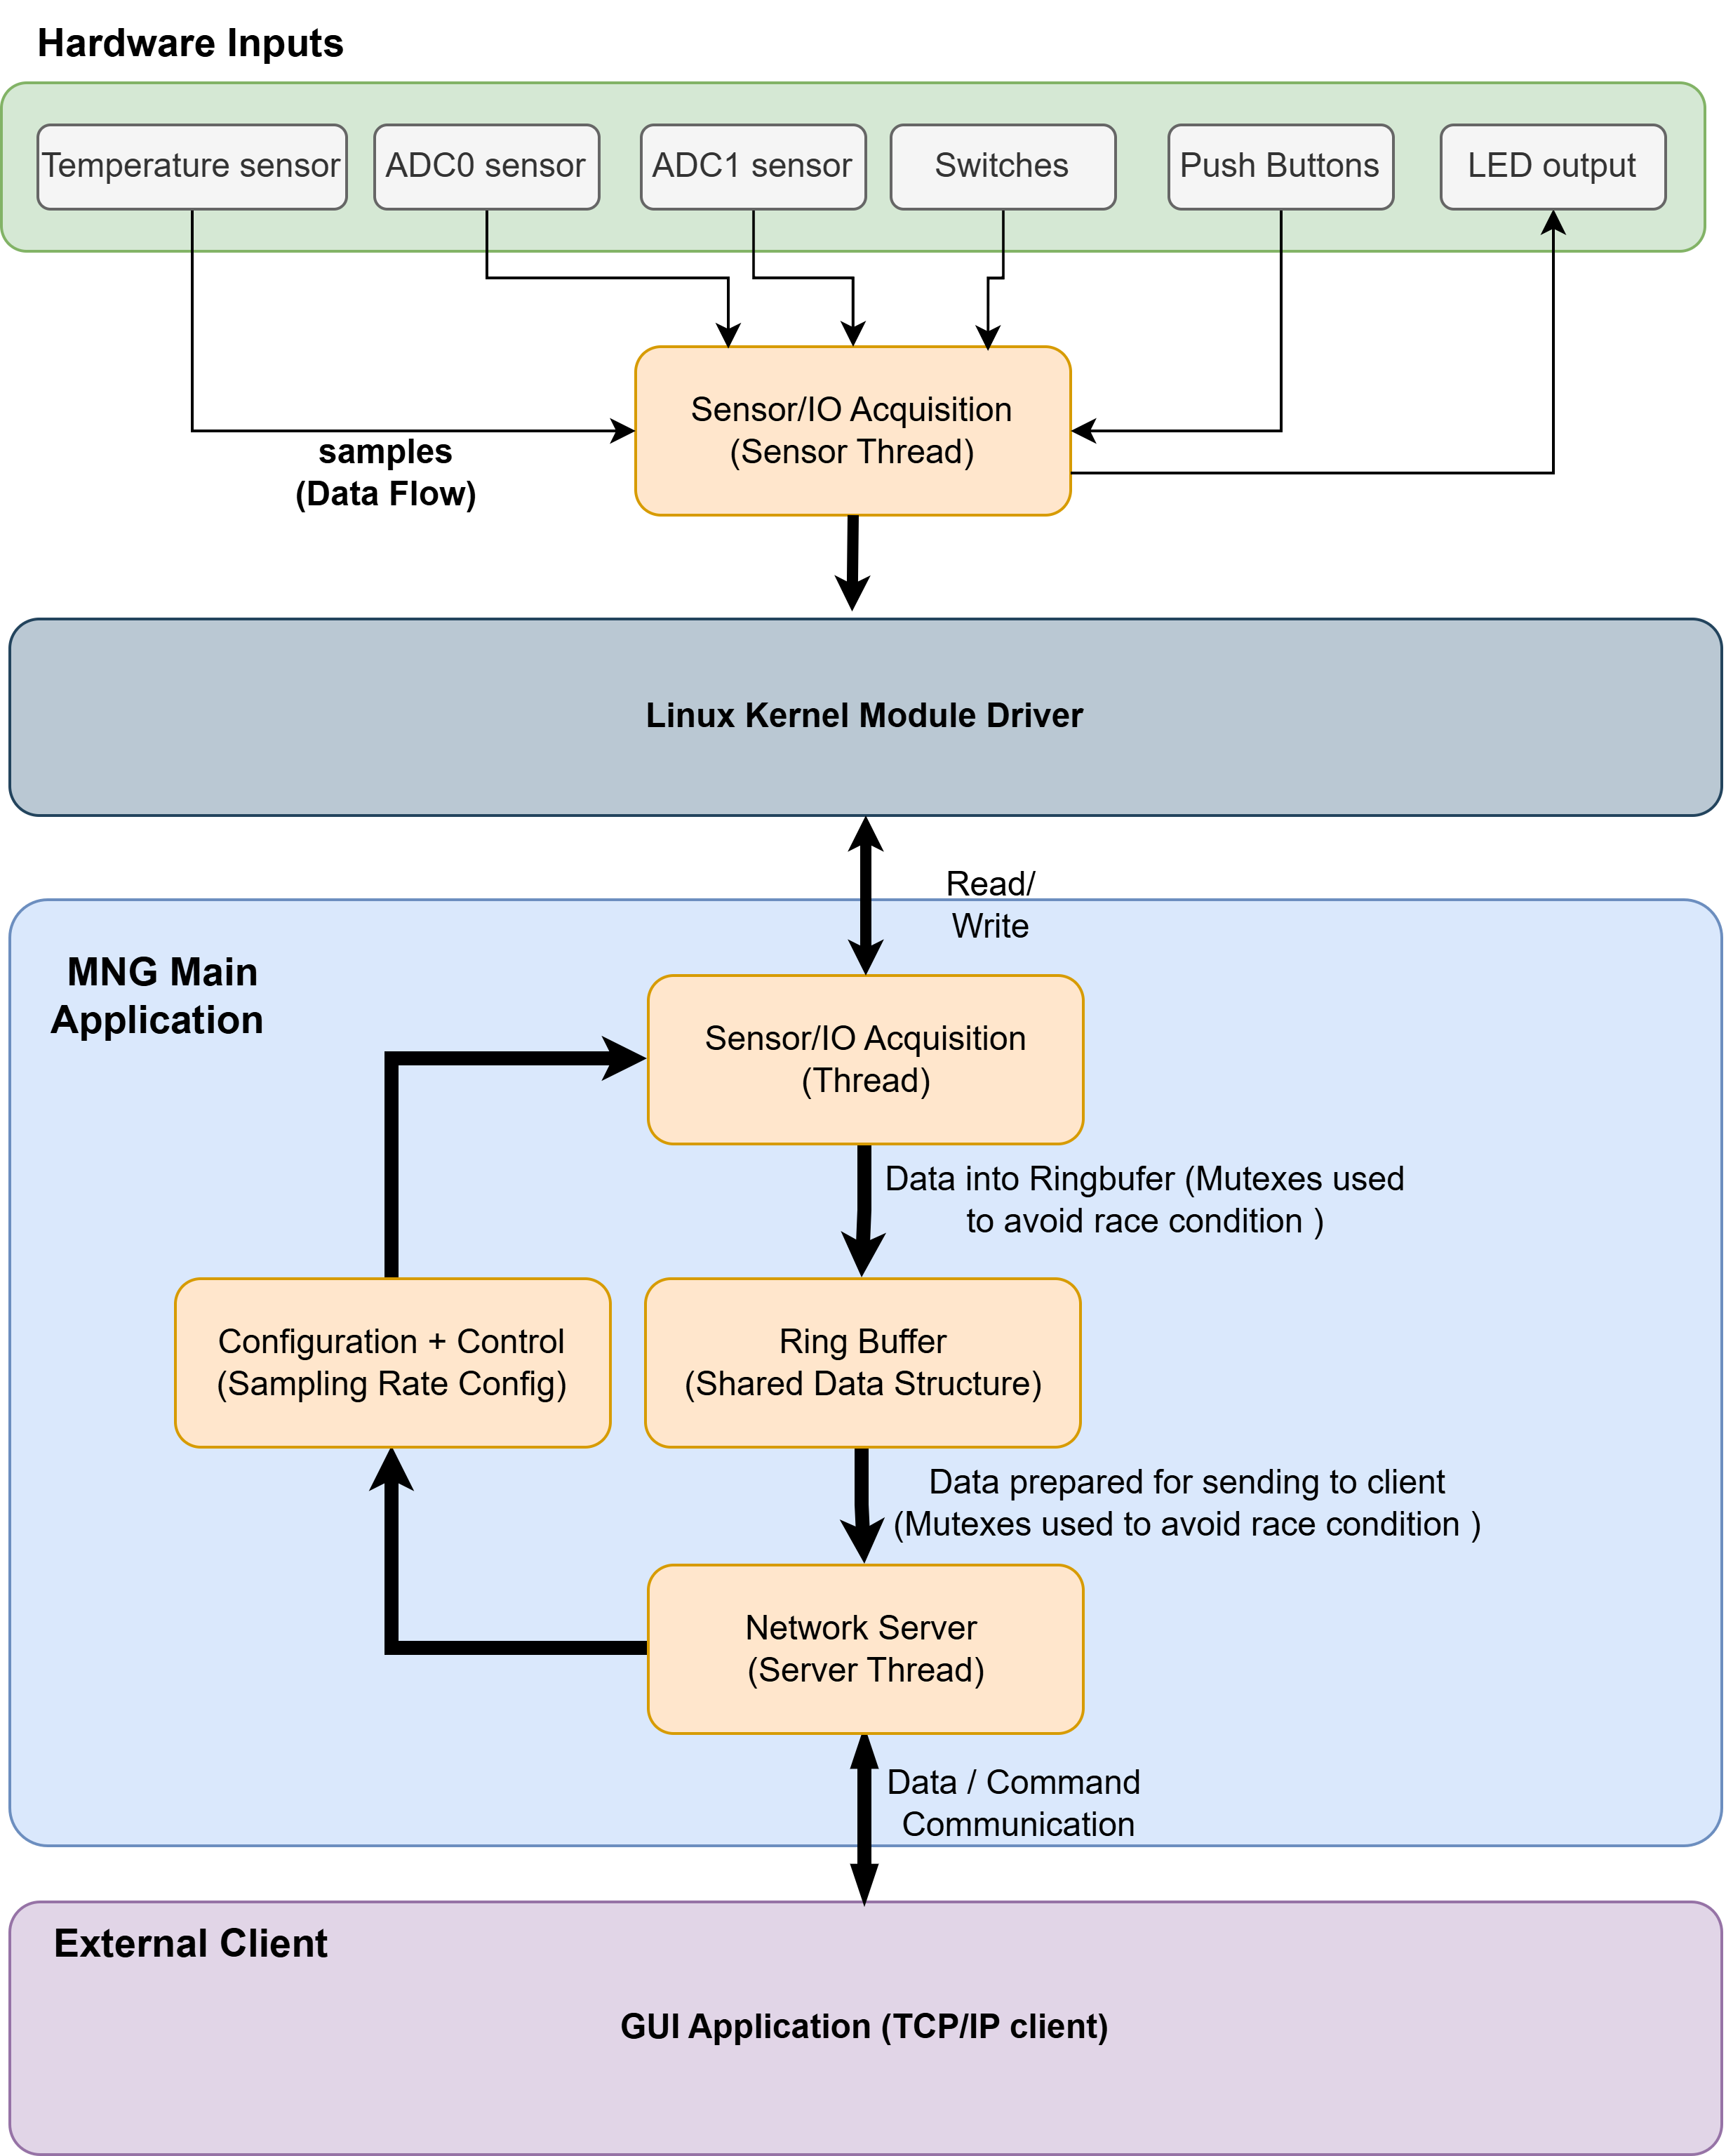
\includegraphics[width = 0.75\textwidth]{media/softArch2.png}
	\caption{Software Architecture of the Measurement Network Gateway}
	\label{fig-softArch}
\end{figure}
The Measurement Network Gateway (MNG) software architecture is designed as a layered and modular system running on an embedded Linux platform based on the Zynq architecture. The design separates hardware interaction, kernel-level driver functionality, user-space application logic, and external client communication to ensure scalability, maintainability, and real-time capable data acquisition.

At the lowest level, multiple sensors and digital inputs (temperature sensor, ADC channels, switches, and push buttons) are connected to the hardware, available throught the IP generated in Vivado Design suite in VHDL language. Based on the custom hardware designed, Petalinux is created and for the custom hardware a Linux Kernel Module was developed. This kernel module encapsulates low-level hardware access and exposes a character device interface \texttt{(/dev/meascdd}) to user space.

The MNG main application operates entirely in user space and follows a multi-threaded design. A dedicated sensor acquisition thread periodically reads data from the device interface and stores sampled values into a thread-safe ring buffer. Synchronization mechanisms such as mutexes and condition variables ensure safe concurrent access between threads.

A separate network server thread retrieves data from the ring buffer and transmits it to an external GUI client via a TCP/IP-based custom communication protocol. In addition to data streaming, the server thread processes configuration and control commands received from the client, such as sampling rate adjustments. A configuration manager component updates system parameters accordingly and propagates them to the acquisition layer.

Overall, the architecture provides a structured and scalable framework for reliable sensor acquisition, real-time processing, and network-based monitoring in embedded Linux environments.

\section{Data acquisition and sensor measurement}
The sensor thread is the core data acquisition component of the Measurement Network Gateway, responsible for continuously reading and timestamping data from all connected sensors at configurable sampling rates. Running as a dedicated POSIX thread, it operates independently from the server thread, ensuring that sensor sampling remains uninterrupted regardless of network activity or client communication state.

Upon startup, the thread attempts to open the hardware device file \texttt{/dev/meascdd} for direct sensor access. If the device is unavailable, the thread automatically falls back to simulation mode, generating synthetic sensor data that mimics real hardware behaviour, allowing the system to be tested and demonstrated without physical hardware. Following device initialisation, the temperature sensor is powered up and all timing references are established using a high-resolution elapsed time counter.

The thread manages five independent sensors --- temperature, two ADC channels, a switch bank, and a push button --- each operating at its own configurable sampling frequency. A deadline-based scheduling approach is employed, where each sensor maintains its own next scheduled sample time, and the thread sleeps only until the nearest upcoming deadline. This design minimises CPU usage while preserving timing accuracy across all channels simultaneously.

The following code show the basic structure of the threads created inside the main application. 
\begin{minted}[bgcolor = lightgray, tabsize = 4, breaklines]{c}
typedef struct {
	pthread_t       thobj;
	pthread_cond_t  thcond;
	pthread_mutex_t thmutex;
	config_struct   th_config;
	short int       thkill;
} thread_struct;
\end{minted}

The initial default sampling rate of all the sensors are set to \SI{300}{\hertz} and when the program starts, then it going to sample all the sensor with this frequency, but when connected to client, it can be changed to the desired sampling rate from the user. 

The following code shows the initial sampling rate configuration of all the sensors: 
\begin{minted}[bgcolor = lightgray, tabsize = 4, breaklines]{c}
config_struct main_config = {
.temp_config   = 300,
.adc0_config   = 300,
.adc1_config   = 300,
.switch_config = 300,
.pushb_config  = 300
};
\end{minted}

At the initial stage of the thread function, the thread opens the device file \texttt{/dev/meascdd} to access the hardware sensors. If the device file cannot be opened (e.g., due to missing hardware or permissions), the thread enters a simulation mode where it generates synthetic sensor data for testing purposes. This fallback mechanism ensures that the application can be developed and demonstrated even in the absence of physical hardware and then the ring buffer is initialized to store the acquired sensor data. The thread also powers up the temperature sensor and initializes timing references for accurate timestamping of samples. Alongside the ring-buffer initialization, the thread also initializes the timer used for timestamping the acquired samples. This timer is typically implemented using a high-resolution clock source (e.g., \texttt{clock\_gettime()} with \texttt{CLOCK\_MONOTONIC}) to provide microsecond precision timestamps for each sensor reading.

Then it check the sampling rates for each sensor and if the sampling rate is zero, then it will not sample that sensor and it will just sleep until the next deadline of the sensors that have non-zero sampling rates. This design allows for dynamic enabling/disabling of individual sensors without affecting the overall thread operation.

Since each sensor should be sampled independently at its own rate, the thread maintains separate timing references for each sensor type. It calculates the next scheduled sample time for each sensor based on the current time and the configured sampling period. The thread then sleeps until the nearest upcoming deadline, ensuring efficient CPU usage while maintaining accurate timing for all sensors. When a sensor's deadline is reached, the thread reads the sensor value from the device file (or generates a simulated value), timestamps it with microsecond precision, and stores it in the shared ring buffer for later retrieval by the server thread. This process continues indefinitely until a termination signal is received.

Due to the requirement of the project that push-buttons and switches shall be used as an auxilary digital inputs, the state of the switches are used to set the LEDs on the ZedBoard. For example, when the first switch is turned on, the first LED will be turned on and when the second switch is turned on, the second LED will be turned on and so on. This provides a simple visual feedback mechanism for the state of the switches.

The following code shows the device file opening, ring-buffer initialization, timer initialization and the MAX31865 temperature sensor power-up: 
\begin{minted}[bgcolor = lightgray, tabsize = 4, breaklines]{c}
	int fd = open("/dev/meascdd", O_RDWR);
    if (fd < 0) {
        simulation = 1;
        printf("Device open failed - simulation mode\n");
    } else {
        printf("Device opened successfully\n");
    }

    InitTimer();
    InitRingBuffer();
\end{minted}

The following code shows the sampling period calculation with zero rate handling. If the user wants to disable reading one of the sensors, then he can set the sampling rate of that sensor to zero and then the thread will not sample that sensor and it will just sleep until the next deadline of the sensors that have non-zero sampling rates. 
\begin{minted}[bgcolor = lightgray, tabsize = 4, breaklines]{c}
	// Get initial timestamps for all sensors
	uint64_t next_temp_time   = GetElapsedTime();
	uint64_t next_adc0_time   = GetElapsedTime();
	uint64_t next_adc1_time   = GetElapsedTime();
	uint64_t next_switch_time = GetElapsedTime();
	uint64_t next_pushb_time  = GetElapsedTime();

	// Calculate sampling periods with zero-rate protection
	uint64_t period_temp_us   = (main_config.temp_config > 0) ? 
								1000000ULL / main_config.temp_config : 0;
	uint64_t period_adc0_us   = (main_config.adc0_config > 0) ? 
								1000000ULL / main_config.adc0_config : 0;
	uint64_t period_adc1_us   = (main_config.adc1_config > 0) ? 
								1000000ULL / main_config.adc1_config : 0;
	uint64_t period_switch_us = (main_config.switch_config > 0) ? 
								1000000ULL / main_config.switch_config : 0;
	uint64_t period_pushb_us  = (main_config.pushb_config > 0) ? 
								1000000ULL / main_config.pushb_config : 0;

	// Track enabled sensors based on non-zero rates
	int temp_enabled   = (main_config.temp_config > 0);
	int adc0_enabled   = (main_config.adc0_config > 0);
	int adc1_enabled   = (main_config.adc1_config > 0);
	int switch_enabled = (main_config.switch_config > 0);
	int pushb_enabled  = (main_config.pushb_config > 0);
\end{minted}

\subsection{Main Sampling Loop Implementation}

The core of the sensor data acquisition system is implemented as an infinite loop that executes a deadline-driven scheduling algorithm for all five sensor types. At the beginning of each iteration, the thread checks for termination signals by examining both the thread-specific kill flag and the global shutdown flag under mutex protection, ensuring safe and coordinated thread termination. The loop then retrieves the current high-resolution timestamp using the \texttt{GetElapsedTime()} function and calculates the nearest upcoming sampling deadline by comparing the next scheduled sampling times of all enabled sensors, selecting the smallest value as the sleep target. A critical safety check handles the scenario where all sensors are disabled (i.e., all sampling rates set to zero), causing the sleep target to remain at \texttt{UINT64\_MAX}; in this case, the thread enters a 10-millisecond sleep before re-evaluating, preventing CPU exhaustion while remaining responsive to shutdown signals. 

When sensors are enabled and the current time precedes the nearest deadline, the thread performs a granular sleep operation, breaking the sleep into small chunks of maximum 100 microseconds. This chunked approach maintains system responsiveness by allowing early wake-up on shutdown signals and enabling timely detection of configuration changes. After waking, the loop sequentially evaluates each enabled sensor to determine if its sampling deadline has been reached; for those that have, the appropriate hardware read or simulation function is invoked, the sampled value is timestamped and pushed to the ring buffer via \texttt{PushRB()}, and the next sampling time is advanced by the configured period. 

Of particular note is the switch-handling logic, which implements a visual feedback mechanism by comparing the current switch state against the last known state stored in a static variable. Only when a state change is detected are the LEDs updated via \texttt{LedWrite()}, ensuring efficient operation by avoiding redundant writes while providing immediate visual confirmation of input state changes. This direct mapping between switch positions and LEDs (switch N controls LED N) offers intuitive feedback without requiring additional software monitoring. The overall architecture ensures precise, jitter-minimized sampling intervals while maintaining system responsiveness and proper synchronization between hardware inputs and visual outputs.
\begin{minted}[bgcolor = lightgray, tabsize = 4, breaklines]{c}
while (1)
{
    // Check for thread termination
    pthread_mutex_lock(&sensor_thread.thmutex);
    int kill = sensor_thread.thkill;
    pthread_mutex_unlock(&sensor_thread.thmutex);
    if (kill || g_shutdown) break;
    
    uint64_t current_time = GetElapsedTime();
    
    // Calculate the nearest upcoming sampling deadline
    uint64_t sleep_target = UINT64_MAX;
    
    if (temp_enabled && next_temp_time < sleep_target) 
        sleep_target = next_temp_time;
    if (adc0_enabled && next_adc0_time < sleep_target) 
        sleep_target = next_adc0_time;
    if (adc1_enabled && next_adc1_time < sleep_target) 
        sleep_target = next_adc1_time;
    if (switch_enabled && next_switch_time < sleep_target) 
        sleep_target = next_switch_time;
    if (pushb_enabled && next_pushb_time < sleep_target) 
        sleep_target = next_pushb_time;
    
    // Handle all-sensors-disabled case
    if (sleep_target == UINT64_MAX) {
        usleep(10000);  // Sleep 10ms and check again
        continue;
    }
    
    // Sleep until the next sampling deadline
    if (current_time < sleep_target) {
        uint64_t sleep_us = sleep_target - current_time;
        while (sleep_us > 0) {
            uint64_t chunk = (sleep_us > 100) ? 100 : sleep_us;
            usleep(chunk);
            sleep_us -= chunk;
            current_time = GetElapsedTime();
            if (current_time >= sleep_target) break;
            if (g_shutdown) break;
        }
    }
    
    if (g_shutdown) break;
    
    // Sample each enabled sensor if its deadline has arrived
    if (temp_enabled && current_time >= next_temp_time) {
        // Read temperature sensor
        int raw = 0;
        if (simulation) {
            raw = (int)(GenerateFakeTemperature(current_time) * 100);
        } else {
            TempRead(fd, &raw);
        }
        PushRB(sid_temp, current_time, (uint32_t)raw);
        next_temp_time += period_temp_us;
    }
    
    // Similar blocks for ADC0, ADC1, switches, and push-buttons...
    
    // Switch-LED feedback mechanism
    if (switch_enabled && current_time >= next_switch_time) {
        uint8_t sw = ReadSwitch(fd);
        static uint8_t LastSwitchState = 0xff;
        
        // Update LEDs only when switch state changes
        if (sw != LastSwitchState) {
            LedWrite(fd, sw);  // Direct mapping: switch N -> LED N
            LastSwitchState = sw;
        }
        PushRB(sid_switches, current_time, sw);
        next_switch_time += period_switch_us;
    }
}
\end{minted}

























\section{Network server implementation}
The Measurement Network Gateway requires a robust communication mechanism to enable remote access to sensor data and configuration control. To fulfill this requirement, a TCP/IP-based server has been implemented as an integral component of the main application. This section presents the design, implementation, and operational characteristics of the network server subsystem.

\subsection{TCP/IP Server Fundamentals}

The Transmission Control Protocol (TCP) is a connection-oriented, reliable transport layer protocol that operates on top of the Internet Protocol (IP). Unlike the User Datagram Protocol (UDP), which provides best-effort delivery, TCP guarantees ordered and error-free delivery of data through mechanisms such as acknowledgments, retransmissions, and flow control. The TCP/IP socket programming interface provides a standardized API for implementing network communication in userspace applications.

A typical TCP server follows a well-defined operational sequence: socket creation, binding to a specific IP address and port, listening for incoming connections, accepting client connections, and finally exchanging data through send and receive operations. This client-server model forms the foundation of most networked applications, from web servers to industrial monitoring systems.

\subsection{Design Rationale for TCP in MNG}

For the Measurement Network Gateway application, TCP was selected over UDP for several critical reasons. First, the reliable delivery guarantee ensures that configuration commands (such as sampling rate updates) and sensor data reach the client without loss or corruption, which is essential for accurate monitoring and control. Second, the connection-oriented nature of TCP provides clear session management, allowing the server to track client connection status and handle disconnections gracefully. Third, the ordered delivery property ensures that timestamped sensor samples arrive in the correct sequence, simplifying client-side processing and visualization.

\subsection{Server Role in the MNG System}

The network server thread acts as the primary interface between the embedded measurement system and external monitoring clients. Its responsibilities include:

\begin{itemize}
	\item Accepting and managing TCP connections from GUI clients and other monitoring tools
	\item Receiving and parsing text-based commands for configuration and control
	\item Retrieving sensor data from the shared ring buffer and transmitting it to connected clients
	\item Coordinating with the sensor acquisition thread through shared configuration structures
	\item Handling connection errors, client disconnections, and graceful shutdown sequences
\end{itemize}

The server operates as an independent pthread within the main application, enabling concurrent sensor acquisition and network communication. Thread-safe access to shared resources (ring buffer and configuration data) is ensured through mutex-based synchronization mechanisms.

\subsection{Server Thread Architecture}
The network server is implemented as a separate POSIX thread (pthread) within the main application, enabling concurrent execution alongside the sensor acquisition thread. This multi-threaded architecture allows the server to handle client communication independently while sensor data continues to be collected in the background without blocking or interference.

The server thread encapsulates all network-related functionality within a single execution context. The thread structure, defined as \texttt{threadstruct} in the main application, contains several essential components:

\begin{itemize}
	\item \texttt{pthread\_t thobj}: The thread object handle used by the pthread library for thread management
	\item \texttt{pthread\_cond\_t thcond}: Condition variable for thread synchronization and signaling
	\item \texttt{pthread\_mutex\_t thmutex}: Mutex for protecting thread-specific shared state
	\item \texttt{config\_struct}: This is the structure used for the sampling rate configuration
	\item \texttt{short int thkill}: Flag for signaling thread termination requests
\end{itemize}

The server thread executes the \texttt{serverthreadfunction()}, which implements the complete TCP server lifecycle from socket initialization through connection handling and graceful shutdown. This function operates in an infinite loop, waiting for and serving client connections until an explicit termination signal is received.

Unlike the sensor thread, which requires configuration parameters to control sampling rates, the server thread operates with a simpler initialization model. Its primary runtime parameters include the TCP port number (defined as \texttt{PORT 50012}) and receive buffer size (\texttt{CMDBUFSIZE 1024} bytes), which are compile-time constants.

To control the data streaming behavior and server operation, a state machine has been implemented using an enumerated type. This state management mechanism allows clients to start, stop, pause, and reconfigure the data stream without disconnecting from the server:

\begin{minted}[bgcolor=lightgray, breaklines, tabsize=4]{c}
	typedef enum {
		STOPPED       = 0,  // Server idle, not streaming data
		RUNNING,            // Actively streaming sensor data to client
		PAUSED,             // Temporarily suspended, maintaining connection
		CONFIGURATION,      // Accepting configuration commands
		DISCONNECT,         // Client-requested disconnect
		SHUTDOWN            // Server shutdown, exit loop entirely
	} stream_state_t;
\end{minted}

Each state represents a distinct operational mode:

\begin{itemize}
	\item \textbf{STOPPED:} The initial state after client connection. The server is connected but not actively transmitting sensor data. It waits for client commands to transition to other states.
	
	\item \textbf{RUNNING:} The server actively retrieves samples from the ring buffer and transmits them to the client. Data streaming continues until a pause, stop, or disconnect command is received.
	
	\item \textbf{PAUSED:} Data streaming is temporarily suspended while maintaining the TCP connection. This allows clients to halt data flow temporarily without losing connection state, useful for GUI operations or processing delays.
	
	\item \textbf{CONFIGURATION:} The server enters a configuration mode where it accepts and processes parameter update commands (e.g., sampling rate changes) without streaming data. This state ensures configuration updates are applied atomically without interfering with data transmission.
	
	\item \textbf{DISCONNECT:} Signals that the client has requested disconnection. The server performs cleanup operations, closes the client socket, and returns to waiting for new connections.
	
	\item \textbf{SHUTDOWN:} Indicates a complete server shutdown request. Unlike DISCONNECT, which only closes the current client connection, SHUTDOWN causes the server thread to exit its main loop entirely, terminating the thread.
\end{itemize}

The server maintains a \texttt{stream\_state\_t} variable that tracks the current state. Client commands trigger state transitions, and the server's behavior in the main loop depends on the current state. This design provides a clean separation between connection management, configuration, and data streaming operations.

The following code shows the structure of each thread created inside the main application: 
\begin{minted}[bgcolor= lightgray, breaklines, tabsize=4]{c}
	typedef struct {
		pthread_t       thobj;
		pthread_cond_t  thcond;
		pthread_mutex_t thmutex;
		config_struct   th_config;
		short int       thkill;
	} thread_struct;
\end{minted}

After definition of the structure of the thread, the server thread can be defined as follows: 

\begin{minted}[bgcolor= lightgray, breaklines, tabsize=4]{c}
thread_struct server_thread;
\end{minted}

\subsubsection{Data Packet Structure}

Sensor data is transmitted to clients using a well-defined binary packet structure. Each packet encapsulates a single sensor sample with its associated metadata:

\begin{minted}[bgcolor=lightgray, breaklines, tabsize=4]{c}
	typedef struct {
		int      sid;      // Sensor ID (1=Temp, 2=ADC0, 3=ADC1, 
						   // 4=Switch, 5=Push-button)
		int      svalue;   // Sensor value (raw reading)
		uint64_t ts;       // Timestamp in microseconds since startup
	} packet;
\end{minted}

This structure, defined as \texttt{packet}, contains three fields totaling 16 bytes (assuming 32-bit integers and 64-bit timestamp on the target platform):

\begin{itemize}
	\item \textbf{sid (Sensor ID):} Identifies which sensor produced the measurement. The sensor ID mapping corresponds to the ring buffer organization: 1 for temperature, 2 for ADC0, 3 for ADC1, 4 for switches, and 5 for push-buttons.
	\item \textbf{svalue (Sensor Value):} The raw sensor reading as retrieved from the hardware. The interpretation of this value depends on the sensor type.
	\item \textbf{ts (Timestamp):} A 64-bit unsigned integer representing microseconds elapsed since the system timer initialization, providing high-precision timing information for each sample.
\end{itemize}


\subsection{Sampling Rate Configuration}
The sensor sampling rates are stored in a shared configuration structure accessible to both the sensor thread (consumer) and the server thread (modifier). To ensure thread-safe access, dedicated functions have been implemented for reading and writing configuration parameters.

\textbf{Configuration Update Function:}

The \texttt{set\_config()} function provides a thread-safe mechanism for updating sampling rate parameters:

\begin{minted}[bgcolor=lightgray, breaklines, tabsize=4]{c}
	void set_config(config_struct *config)
	{
		pthread_mutex_lock(&server_thread.thmutex);
		main_config.temp_config   = config->temp_config;
		main_config.adc0_config   = config->adc0_config;
		main_config.adc1_config   = config->adc1_config;
		main_config.switch_config = config->switch_config;
		main_config.pushb_config  = config->pushb_config;
		pthread_mutex_unlock(&server_thread.thmutex);
	}
\end{minted}

This function accepts a pointer to a \texttt{config\_struct} containing the new sampling rate values (in microseconds) for each sensor type. The entire update operation is protected by the server thread's mutex (\texttt{server\_thread.thmutex}) to prevent race conditions when the sensor thread is reading these values. By locking the mutex, the function guarantees atomic updates of all five configuration parameters, ensuring the sensor thread never observes a partially-updated configuration state.

\textbf{Configuration Display Function:}

For debugging and verification purposes, the \texttt{print\_config()} function outputs the current configuration to the console:

\begin{minted}[bgcolor=lightgray, breaklines, tabsize=4]{c}
	void print_config(void)
	{
		printf("temp_config:     %u\n", main_config.temp_config);
		printf("adc0_config:     %u\n", main_config.adc0_config);
		printf("adc1_config:     %u\n", main_config.adc1_config);
		printf("switches_config: %u\n", main_config.switch_config);
		printf("pushb_config:    %u\n", main_config.pushb_config);
	}
\end{minted}

This function prints all sampling period values in microseconds. While not mutex-protected (as it's a read-only operation for display purposes), it provides valuable runtime visibility into the current system configuration.

When a client sends a configuration command over the network, the server thread parses the command, extracts the new sampling rate values, populates a \texttt{config\_struct}, and calls \texttt{set\_config()} to apply the changes. The sensor thread, which continuously checks the \texttt{main\_config} structure in its acquisition loop, automatically adopts the new sampling rates for subsequent sensor reads without requiring a restart.

This design enables dynamic runtime reconfiguration of the measurement system, allowing clients to optimize sampling rates based on real-time requirements or system load conditions.

%start of the server thread function 


\subsection{TCP Socket Implementation}

\subsubsection{Thread Function Initialization}

The server thread function begins execution by initializing essential variables and data structures required for network communication and data transmission. This initialization phase prepares all necessary resources before socket creation:

\begin{minted}[bgcolor=lightgray, breaklines, tabsize=4]{c}
	void *server_thread_function(void *arg)
	{
		(void)arg;  // Unused parameter
		packet payload[96];
		char   receive_command[CMD_BUF_SIZE];
		
		struct sockaddr_in server_address, client_addr;
		socklen_t client_addr_len = sizeof(client_addr);
		
		stream_state = PAUSED;
		// ... continue with socket creation
	}
\end{minted}

\textbf{Function Parameter:}

The function signature follows the POSIX pthread convention, accepting a \texttt{void *arg} parameter that can be used to pass initialization data to the thread. In this implementation, no configuration parameters are required by the server thread, so the argument is explicitly cast to \texttt{(void)arg} to suppress compiler warnings about unused parameters.

\textbf{Data Transmission Buffer:}

\begin{minted}[bgcolor=lightgray, breaklines, tabsize=4]{c}
	packet payload[96];
\end{minted}

A fixed-size array of 96 \texttt{packet} structures is allocated on the stack for batch data transmission. Each \texttt{packet} contains sensor ID, timestamp, and value fields (16 bytes total), resulting in a payload buffer of \texttt{1536 bytes (1.5 KB)}. This size represents a trade-off between:

\begin{itemize}
	\item Memory consumption on the embedded platform
	\item Network transmission efficiency (larger batches reduce per-packet overhead)
	\item Response latency (smaller batches provide faster initial response)
\end{itemize}

The value of 96 was chosen empirically to provide efficient bulk data transfer while remaining within reasonable stack memory limits.

\textbf{Command Reception Buffer:}

\begin{minted}[bgcolor=lightgray, breaklines, tabsize=4]{c}
	char receive_command[CMD_BUF_SIZE];
\end{minted}

A character buffer of size \texttt{CMD\_BUF\_SIZE} (1024 bytes) is allocated for receiving text-based commands from clients. This size is sufficient for all supported commands, including the \texttt{configure} command which contains five unsigned integer values plus the command keyword.

\textbf{Socket Address Structures:}

\begin{minted}[bgcolor=lightgray, breaklines, tabsize=4]{c}
	struct sockaddr_in server_address, client_addr;
	socklen_t client_addr_len = sizeof(client_addr);
\end{minted}

Two \texttt{sockaddr\_in} structures are declared:
\begin{itemize}
	\item \texttt{server\_address}: Stores the server's binding address (IP and port)
	\item \texttt{client\_addr}: Populated by \texttt{accept()} with the connecting client's address information
\end{itemize}

The \texttt{client\_addr\_len} variable holds the size of the client address structure, required by the \texttt{accept()} system call.

\textbf{Initial Stream State:}

\begin{minted}[bgcolor=lightgray, breaklines, tabsize=4]{c}
	stream_state = PAUSED;
\end{minted}

The global stream state is explicitly set to \texttt{PAUSED} at thread startup. This ensures that when a client connects, the server does not immediately begin streaming data. Instead, it waits for explicit commands from the client (such as \texttt{start}) before transmitting sensor samples. This design provides the client with full control over data flow timing.

Following these initialization steps, the server proceeds to create and configure the listening socket.

\subsubsection{Socket Creation and Configuration}
Upon thread startup, the server thread function begins by creating a TCP socket and configuring it for proper operation. The socket is created using the standard POSIX socket API:

\begin{minted}[bgcolor=lightgray, breaklines, tabsize=4]{c}
	int server_sock = socket(AF_INET, SOCK_STREAM, 0);
	if (server_sock < 0) { 
		perror("socket"); 
		return NULL; 
	}
\end{minted}
The \texttt{socket()} function is called with three arguments:
\begin{itemize}
	\item \texttt{AF\_INET}: Specifies the IPv4 address family
	\item \texttt{SOCK\_STREAM}: Indicates a TCP connection-oriented socket (as opposed to \texttt{SOCK\_DGRAM} for UDP)
	\item \texttt{0}: Lets the system choose the appropriate protocol (TCP for stream sockets)
\end{itemize}

If socket creation fails (returns a negative value), an error message is printed and the thread terminates, preventing further execution with an invalid socket descriptor.

Following socket creation, the \texttt{SO\_REUSEADDR} socket option is enabled:

\begin{minted}[bgcolor=lightgray, breaklines, tabsize=4]{c}
	int opt = 1;
	setsockopt(server_sock, SOL_SOCKET, SO_REUSEADDR, 
	&opt, sizeof(opt));
\end{minted}

This option is critical during development and testing. By default, when a TCP server closes, the operating system keeps the port in a TIME\_WAIT state for several minutes to ensure all delayed packets are properly handled. The \texttt{SO\_REUSEADDR} option allows immediate rebinding to the same port after server restart, preventing "Address already in use" errors. This is particularly useful when repeatedly testing and restarting the server during development without having to wait for the TIME\_WAIT period to expire.


\subsubsection{Address Binding and Port Assignment}

After socket creation and configuration, the server must bind the socket to a specific network address and port number. This process associates the socket with a particular interface and port that clients will use to connect.

The server address structure is initialized and populated:

\begin{minted}[bgcolor=lightgray, breaklines, tabsize=4]{c}
	struct sockaddr_in server_address;
	
	memset(&server_address, 0, sizeof(server_address));
	server_address.sin_family      = AF_INET;
	server_address.sin_addr.s_addr = INADDR_ANY;
	server_address.sin_port        = htons(PORT);
\end{minted}

The \texttt{sockaddr\_in} structure contains three key fields:

\begin{itemize}
	\item \textbf{sin\_family}: Set to \texttt{AF\_INET} to match the socket's address family (IPv4)
	\item \textbf{sin\_addr.s\_addr}: Set to \texttt{INADDR\_ANY} (0.0.0.0), which instructs the server to listen on all available network interfaces. This means the server accepts connections from any interface, whether Ethernet, loopback (127.0.0.1), or any other configured network adapter on the ZedBoard
	\item \textbf{sin\_port}: Set to port 50012 (defined by the \texttt{PORT} constant) using \texttt{htons()} to convert from host byte order to network byte order (big-endian)
\end{itemize}

The binding operation associates this address information with the socket:

\begin{minted}[bgcolor=lightgray, breaklines, tabsize=4]{c}
	if (bind(server_sock, (struct sockaddr *)&server_address,
	sizeof(server_address)) < 0) {
		perror("bind"); 
		close(server_sock); 
		return NULL;
	}
\end{minted}

If binding fails (e.g., the port is already in use by another process, or insufficient permissions), the error is logged, the socket is closed to release resources, and the thread terminates. Port 50012 was selected as it falls within the dynamic/private port range (49152-65535), avoiding conflicts with well-known services and reducing the likelihood of permission issues.

\subsubsection{Listen Mode and Connection Queue}

After successful binding, the socket must be placed in listening mode to accept incoming client connections. This is accomplished with the \texttt{listen()} system call:

\begin{minted}[bgcolor=lightgray, breaklines, tabsize=4]{c}
	if (listen(server_sock, 1) < 0) {
		perror("listen"); 
		close(server_sock); 
		return NULL;
	}
\end{minted}

The \texttt{listen()} function takes two parameters:
\begin{itemize}
	\item \textbf{server\_sock}: The bound socket descriptor
	\item \textbf{backlog (1)}: The maximum length of the queue for pending connections
\end{itemize}

The backlog parameter is set to 1, which means the operating system will queue at most one pending connection request. This value is consistent with the server's single-client sequential architecture. When a client is already connected and being served, any additional connection attempts are either queued (if the queue is empty) or rejected (if the queue is full).

In practice, with a backlog of 1:
\begin{itemize}
	\item If no client is connected, the first connection attempt succeeds immediately
	\item If one client is connected and actively being served, a second connection attempt may be queued
	\item A third connection attempt will likely be rejected by the operating system
\end{itemize}

After successful \texttt{listen()}, the socket is ready to accept connections. The server also publishes the server socket descriptor to a global variable for potential access by the shutdown handler:

\begin{minted}[bgcolor=lightgray, breaklines, tabsize=4]{c}
	pthread_mutex_lock(&g_socket_lock);
	g_server_socket = server_sock;
	pthread_mutex_unlock(&g_socket_lock);
	
	printf("Server listening on port %d\n", PORT);
\end{minted}

This mutex-protected assignment ensures thread-safe access to the socket descriptor, which is important if the shutdown mechanism needs to forcibly close the socket from another execution context.

\subsubsection{Client Connection Acceptance}

With the server socket in listening mode, the outer loop of the server thread function continuously waits for incoming client connections using the \texttt{accept()} system call:

\begin{minted}[bgcolor=lightgray, breaklines, tabsize=4]{c}
	while (!g_shutdown)
	{
		printf("Waiting for client...\n");
		
		int client_sock = accept(server_sock,
		(struct sockaddr *)&client_addr,
		&client_addr_len);
		if (client_sock < 0) {
			if (g_shutdown) break;
			perror("accept");
			continue;
		}
		
		printf("Client connected\n");
		// ... proceed to serve client
	}
\end{minted}

The \texttt{accept()} call is a blocking operation that suspends the thread until a client initiates a connection. When a connection request arrives, \texttt{accept()} performs the TCP three-way handshake, establishes the connection, and returns a new socket descriptor (\texttt{client\_sock}) dedicated to communication with that specific client.

Key aspects of the acceptance process:

\begin{itemize}
	\item \textbf{Blocking behavior}: The thread remains blocked at \texttt{accept()} until a client connects or the socket is closed
	\item \textbf{Client information}: The \texttt{client\_addr} structure is populated with the client's IP address and port number, though this information is not currently used for access control or logging
	\item \textbf{Error handling}: If \texttt{accept()} fails, the server checks whether failure was due to shutdown (socket closed intentionally); otherwise, it logs the error and continues waiting for the next connection attempt
	\item \textbf{Sequential service}: Once a client is accepted, the server enters the inner loop to serve that client exclusively until disconnection
\end{itemize}

After accepting a connection, the client socket descriptor is published to a global variable for potential access during shutdown:

\begin{minted}[bgcolor=lightgray, breaklines, tabsize=4]{c}
	pthread_mutex_lock(&g_socket_lock);
	g_client_socket = client_sock;
	pthread_mutex_unlock(&g_socket_lock);
\end{minted}

The stream state is also reset to \texttt{PAUSED}, ensuring the server starts in a known state where it awaits commands without automatically streaming data.


\subsection{Client Connection Management}

\subsubsection{Single-Client Connection Model}

The server implements a **sequential single-client architecture**, meaning it serves only one client at a time. This design is reflected in both the socket configuration (listen backlog of 1) and the dual-loop structure of the server thread function.

The outer loop continuously accepts new client connections in sequence:

\begin{minted}[bgcolor=lightgray, breaklines, tabsize=4]{c}
	while (!g_shutdown)
	{
		printf("Waiting for client...\n");
		
		int client_sock = accept(server_sock,
		(struct sockaddr *)&client_addr,
		&client_addr_len);
		// ... serve client in inner loop
	}
\end{minted}

This architecture provides several advantages for the MNG application:

\begin{itemize}
	\item \textbf{Simplified resource management}: A single client eliminates the need for complex per-client state management and thread pools
	\item \textbf{Predictable data flow}: The ring buffer has only one consumer (the server serving one client), simplifying synchronization
	\item \textbf{Deterministic behavior}: System performance and response times are consistent and easy to debug
	\item \textbf{Application requirements}: The primary use case is a single GUI client monitoring the gateway; multiple simultaneous clients are not required
	\item \textbf{Resource constraints}: The embedded ZedBoard platform has limited processing power and memory; serving multiple concurrent clients would increase CPU load and complicate buffer management
\end{itemize}

When a client is connected and being served, any additional connection attempts must wait until the current client disconnects. The server does not support concurrent multi-client connections.

\subsubsection{Connection Establishment}

The outer loop implements the connection acceptance and sequential client handling logic. After successfully entering listening mode, the server enters a continuous loop that waits for and serves clients one at a time:

\begin{minted}[bgcolor=lightgray, breaklines, tabsize=4]{c}
	while (!g_shutdown)
	{
		printf("Waiting for client...\n");
		
		int client_sock = accept(server_sock,
		(struct sockaddr *)&client_addr,
		&client_addr_len);
		if (client_sock < 0) {
			if (g_shutdown) break;
			perror("accept");
			continue;
		}
		
		/* Publish client fd */
		pthread_mutex_lock(&g_socket_lock);
		g_client_socket = client_sock;
		pthread_mutex_unlock(&g_socket_lock);
		
		printf("Client connected\n");
		stream_state = PAUSED;
		
		/* ---- INNER LOOP: serve one client ---- */
		// ... command processing loop
	}
\end{minted}

\textbf{Blocking Accept:}

The \texttt{accept()} call is a blocking operation that suspends the server thread until a client initiates a TCP connection. During this time, the thread consumes no CPU resources. When a connection request arrives, the operating system completes the TCP three-way handshake and \texttt{accept()} returns a new socket descriptor (\texttt{client\_sock}) dedicated to communication with that specific client.

\textbf{Error Handling:}

If \texttt{accept()} returns a negative value, indicating an error, the server performs two checks:

\begin{enumerate}
	\item \textbf{Shutdown check}: If \texttt{g\_shutdown} is set, the error is expected (the listening socket was closed intentionally by \texttt{request\_shutdown()}), and the loop exits cleanly with \texttt{break}
	\item \textbf{Other errors}: If not a shutdown scenario, the error is logged with \texttt{perror()}, and the loop continues with \texttt{continue}, returning to wait for the next connection attempt
\end{enumerate}

This error handling ensures the server remains robust against transient network errors while responding appropriately to intentional shutdown requests.

\textbf{Client Socket Registration:}

Upon successful connection acceptance, the client socket descriptor is stored in the global variable \texttt{g\_client\_socket} within a mutex-protected critical section:

\begin{minted}[bgcolor=lightgray, breaklines, tabsize=4]{c}
	pthread_mutex_lock(&g_socket_lock);
	g_client_socket = client_sock;
	pthread_mutex_unlock(&g_socket_lock);
\end{minted}

This registration serves two purposes:
\begin{itemize}
	\item Allows the \texttt{request\_shutdown()} function to access and close the client socket from a different execution context
	\item Provides thread-safe access to the socket descriptor for potential monitoring or diagnostic purposes
\end{itemize}

\textbf{Initial State Configuration:}

After registering the client socket, the stream state is reset to \texttt{PAUSED}:

\begin{minted}[bgcolor=lightgray, breaklines, tabsize=4]{c}
	stream_state = PAUSED;
\end{minted}

This ensures each newly connected client starts in a known state where the server awaits commands without automatically streaming data. The client must explicitly issue a \texttt{start} command to begin receiving sensor data, providing full control over data flow timing.

Following these initialization steps, execution proceeds to the inner loop where the server receives and processes commands from the connected client.

\subsubsection{Disconnect Handling and Cleanup}

Client disconnection can occur through three mechanisms: graceful client-initiated disconnect, explicit disconnect command, or connection failure. The server handles all scenarios and performs appropriate cleanup before returning to the outer loop to await the next client.

\textbf{Normal Disconnection:}

When \texttt{recv()} returns 0 in the inner loop, it indicates the client closed the connection gracefully (TCP FIN received). The inner loop exits with \texttt{break}, and execution continues in the outer loop's cleanup section:

\begin{minted}[bgcolor=lightgray, breaklines, tabsize=4]{c}
	/* Clean up client socket if not already closed */
	pthread_mutex_lock(&g_socket_lock);
	if (g_client_socket >= 0) {
		close(g_client_socket);
		g_client_socket = -1;
	}
	pthread_mutex_unlock(&g_socket_lock);
\end{minted}

\textbf{Command-Initiated Disconnect:}

When the client sends a \texttt{disconnect} command, the stream state is set to \texttt{DISCONNECT}, triggering the following cleanup sequence in the inner loop:

\begin{minted}[bgcolor=lightgray, breaklines, tabsize=4]{c}
	if (stream_state == DISCONNECT) {
		printf("Closing client connection\n");
		shutdown(client_sock, SHUT_RDWR);
		close(client_sock);
		
		pthread_mutex_lock(&g_socket_lock);
		g_client_socket = -1;
		pthread_mutex_unlock(&g_socket_lock);
		break;  /* go back to accept() */
	}
\end{minted}

The \texttt{shutdown()} call with \texttt{SHUT\_RDWR} disables both send and receive operations on the socket, informing the peer of the intentional closure. The socket is then closed with \texttt{close()}, releasing system resources. The global client socket variable is reset to -1 (invalid descriptor) to indicate no client is connected.

\textbf{Return to Accept Loop:}

After cleanup, the inner loop exits with \texttt{break}, returning execution to the outer loop's \texttt{accept()} call. The server is now ready to accept a new client connection, completing the sequential client service cycle.

This architecture ensures clean resource management and allows the server to serve multiple clients sequentially over its lifetime without requiring restart.


\subsection{Command Protocol and Communication}

\subsubsection{Command Receive Loop Implementation}

The inner loop continuously monitors for incoming commands from the connected client using non-blocking I/O:

\begin{minted}[bgcolor=lightgray, breaklines, tabsize=4]{c}
	while (!g_shutdown)
	{
		memset(receive_command, 0, CMD_BUF_SIZE);
		int n = recv(client_sock, receive_command, 
		CMD_BUF_SIZE - 1, MSG_DONTWAIT);
		
		if (n > 0) {
			// Process command
		} else if (n == 0) {
			// Client disconnected
			break;
		} else {
			// Handle errors
		}
		
		usleep(1000);  /* light pacing */
	}
\end{minted}

\textbf{Non-Blocking Receive:}

The \texttt{MSG\_DONTWAIT} flag makes \texttt{recv()} non-blocking, allowing the loop to check for shutdown signals and state changes without indefinitely waiting for data. If no data is available, \texttt{recv()} returns -1 with \texttt{errno} set to \texttt{EAGAIN} or \texttt{EWOULDBLOCK}.

\textbf{Buffer Management:}

The receive buffer is cleared with \texttt{memset()} before each receive operation to prevent data from previous commands from contaminating new commands. The receive size is limited to \texttt{CMD\_BUF\_SIZE - 1} to reserve space for null termination.

\textbf{Loop Pacing:}

A 1-millisecond sleep (\texttt{usleep(1000)}) at the end of each iteration prevents the loop from consuming 100\% CPU while polling. This provides a balance between responsiveness (1ms maximum latency) and CPU efficiency.

\subsubsection{Command Parsing and String Termination}

When data is received (\texttt{n > 0}), the command string is properly terminated and sanitized:

\begin{minted}[bgcolor=lightgray, breaklines, tabsize=4]{c}
	receive_command[n] = '\0';
	for (char *p = receive_command; *p; p++)
	if (*p == '\n' || *p == '\r') { *p = '\0'; break; }
	
	printf("Command: [%s]\n", receive_command);
\end{minted}

This two-step termination ensures:
\begin{enumerate}
	\item The buffer is null-terminated at the received data boundary
	\item Any newline or carriage return characters within the command are replaced with null terminators, effectively trimming the command string
\end{enumerate}

This handles commands sent from various clients that may use different line endings (LF, CR, or CRLF).

\subsubsection{Supported Command Set}

The server implements five commands, each triggering specific behavior:

\textbf{1. start Command - Batch Data Transmission:}

\begin{minted}[bgcolor=lightgray, breaklines, tabsize=4]{c}
	if (!strcmp(receive_command, "start"))
	{
		int available;
		pthread_mutex_lock(&server_thread.thmutex);
		available = Ring_Buf.rb_cnt;
		pthread_mutex_unlock(&server_thread.thmutex);
		
		if (available > 0) {
			int to_send = (available >= 96) ? 96 : available;
			for (int i = 0; i < to_send; i++) {
				if (PopRB(&payload[i].sid, &payload[i].ts,
				&payload[i].svalue) < 0) {
					to_send = i;
					break;
				}
			}
			if (to_send > 0) {
				ssize_t sent = send(client_sock, payload,
				to_send * sizeof(packet), 0);
				if (sent <= 0) { perror("send"); break; }
				printf("Sent %d packets\n", to_send);
			}
		}
		stream_state = PAUSED;
	}
\end{minted}

The \texttt{start} command retrieves available samples from the ring buffer and sends them as a batch. Up to 96 packets are sent per request, implementing a request-response data delivery model rather than continuous streaming.

\textbf{2. pause/stop Commands - Stream Control:}

\begin{minted}[bgcolor=lightgray, breaklines, tabsize=4]{c}
	else if (!strcmp(receive_command, "pause") ||
	!strcmp(receive_command, "stop"))
	{
		stream_state = PAUSED;
		printf("%s acknowledged\n", receive_command);
	}
\end{minted}

These commands set the stream state to \texttt{PAUSED}. In the current implementation (request-response model), this primarily serves as an acknowledgment.

\textbf{3. configure Command - Sampling Rate Update:}

\begin{minted}[bgcolor=lightgray, breaklines, tabsize=4]{c}
	else if (!strncmp(receive_command, "configure ", 10))
	{
		config_struct cfg;
		int parsed = sscanf(&receive_command[10], "%u %u %u %u %u",
		&cfg.temp_config, &cfg.adc0_config,
		&cfg.adc1_config, &cfg.switch_config,
		&cfg.pushb_config);
		if (parsed == 5) { 
			set_config(&cfg); 
			print_config(); 
		}
		else printf("Bad configure arguments\n");
	}
\end{minted}

The configure command accepts five space-separated unsigned integers representing sampling periods in microseconds for temperature, ADC0, ADC1, switches, and push-buttons. The \texttt{sscanf()} return value is checked to ensure all five parameters were successfully parsed.

\textbf{4. disconnect Command - Client Disconnection:}

\begin{minted}[bgcolor=lightgray, breaklines, tabsize=4]{c}
	else if (!strcmp(receive_command, "disconnect"))
	{
		printf("Client requested disconnect\n");
		stream_state = DISCONNECT;
	}
\end{minted}

Sets the state to \texttt{DISCONNECT}, triggering cleanup logic later in the loop.

\textbf{5. shutdown Command - Server Termination:}

\begin{minted}[bgcolor=lightgray, breaklines, tabsize=4]{c}
	else if (!strcmp(receive_command, "shutdown"))
	{
		printf("Shutdown command received — stopping server\n");
		stream_state = SHUTDOWN;
		
		shutdown(client_sock, SHUT_RDWR);
		close(client_sock);
		
		pthread_mutex_lock(&g_socket_lock);
		g_client_socket = -1;
		pthread_mutex_unlock(&g_socket_lock);
		
		request_shutdown();
		
		pthread_mutex_lock(&sensor_thread.thmutex);
		sensor_thread.thkill = 1;
		pthread_mutex_unlock(&sensor_thread.thmutex);
		
		goto server_exit;
	}
\end{minted}

Unlike \texttt{disconnect}, the \texttt{shutdown} command terminates the entire server thread and signals the sensor thread to stop. It uses \texttt{goto server\_exit} to break out of both nested loops.

\textbf{Unknown Commands:}

\begin{minted}[bgcolor=lightgray, breaklines, tabsize=4]{c}
	else
	{
		printf("Unknown command: [%s]\n", receive_command);
	}
\end{minted}

Unrecognized commands are logged but do not trigger errors or disconnection, providing robustness against typos or protocol extensions.

\subsection{Data Transmission Strategy}

\subsubsection{Batch Data Retrieval from Ring Buffer}

When the \texttt{start} command is received, the server checks ring buffer availability and retrieves up to 93 samples:

[Include the start command code explanation already provided above, with additional detail:]

\begin{enumerate}
	\item \textbf{Check availability}: Query \texttt{Ring\_Buf.rb\_cnt} with mutex protection
	\item \textbf{Determine batch size}: Minimum of available samples and 93
	\item \textbf{Pop samples}: Call \texttt{PopRB()} for each packet, handling early termination if buffer becomes empty
	\item \textbf{Transmit batch}: Send entire payload array in one \texttt{send()} call
\end{enumerate}

\subsubsection{Binary Packet Transmission}

The payload is transmitted as a contiguous binary blob:

\begin{minted}[bgcolor=lightgray, breaklines, tabsize=4]{c}
	ssize_t sent = send(client_sock, payload,
	to_send * sizeof(packet), 0);
\end{minted}

This sends \texttt{to\_send} packets (each 16 bytes) in a single system call, minimizing overhead. The client must receive and parse this binary data accordingly.

\subsection{Error Handling and Robustness}

\subsubsection{Receive Error Handling}

The inner loop handles three \texttt{recv()} return scenarios:

\begin{minted}[bgcolor=lightgray, breaklines, tabsize=4]{c}
	if (n > 0) {
		// Data received, process command
	}
	else if (n == 0) {
		printf("Client disconnected\n");
		break;  // Exit inner loop
	}
	else {
		if (errno != EAGAIN && errno != EWOULDBLOCK && errno != EINTR) {
			perror("recv");
			break;
		}
	}
\end{minted}

\begin{itemize}
	\item \textbf{n > 0}: Data received successfully, process as command
	\item \textbf{n == 0}: Peer closed connection gracefully (TCP FIN), exit inner loop
	\item \textbf{n < 0}: Error occurred; ignore expected non-blocking errors (\texttt{EAGAIN}, \texttt{EWOULDBLOCK}, \texttt{EINTR}), but log and exit on genuine errors
\end{itemize}

\subsubsection{Disconnect State Handling}

After command processing, the loop checks for disconnect state:

\begin{minted}[bgcolor=lightgray, breaklines, tabsize=4]{c}
	if (stream_state == DISCONNECT) {
		printf("Closing client connection\n");
		shutdown(client_sock, SHUT_RDWR);
		close(client_sock);
		
		pthread_mutex_lock(&g_socket_lock);
		g_client_socket = -1;
		pthread_mutex_unlock(&g_socket_lock);
		break;
	}
\end{minted}

This deferred cleanup approach allows the command handler to set the state, and the main loop performs orderly shutdown.

\subsubsection{Client Socket Cleanup}

After exiting the inner loop, final cleanup ensures the client socket is closed:

\begin{minted}[bgcolor=lightgray, breaklines, tabsize=4]{c}
	pthread_mutex_lock(&g_socket_lock);
	if (g_client_socket >= 0) {
		close(g_client_socket);
		g_client_socket = -1;
	}
	pthread_mutex_unlock(&g_socket_lock);
\end{minted}

The check for \texttt{>= 0} handles cases where the socket was already closed (e.g., during disconnect or shutdown command processing).

\subsection{Shutdown Mechanism and Thread Termination}

\subsubsection{Server Exit Path}

The \texttt{server\_exit} label provides a single exit point for complete server shutdown:

\begin{minted}[bgcolor=lightgray, breaklines, tabsize=4]{c}
	server_exit:
	pthread_mutex_lock(&g_socket_lock);
	if (g_server_socket >= 0) {
		close(g_server_socket);
		g_server_socket = -1;
	}
	pthread_mutex_unlock(&g_socket_lock);
	
	printf("Server thread exiting\n");
	return NULL;
\end{minted}

This cleanup:
\begin{itemize}
	\item Closes the listening socket if not already closed by \texttt{request\_shutdown()}
	\item Resets the global socket descriptor
	\item Logs thread termination
	\item Returns NULL to complete thread execution
\end{itemize}

\subsubsection{Coordinated System Shutdown}

The \texttt{shutdown} command triggers coordinated termination:
\begin{enumerate}
	\item Close client socket gracefully
	\item Call \texttt{request\_shutdown()} to set \texttt{g\_shutdown} flag and close server socket
	\item Signal sensor thread to stop via \texttt{sensor\_thread.thkill}
	\item Jump to \texttt{server\_exit} for final cleanup
\end{enumerate}

This ensures both threads terminate cleanly and all resources are released.


\section{Performance Evaluation and Analysis}
Having established the server implementation details, this section evaluates the performance characteristics of the Measurement Network Gateway server under various operational conditions. Performance evaluation is essential for validating that the system meets real-time requirements and can sustain continuous operation without degradation. The evaluation encompasses throughput analysis, latency measurements, resource utilization, and system behavior under different load conditions.

\subsection{Batch Transmission Buffer Design}

\subsubsection{TCP/IP Maximum Segment Size Considerations}

The selection of 96 packets for the payload buffer is directly derived from TCP/IP protocol frame transmission characteristics. In the TCP/IP protocol, if the data to be sent is 1.5 KB or less, it will be transmitted in a single frame. However, if the data exceeds 1.5 KB, the TCP/IP protocol will divide it into several frames and transmit them sequentially. Since each sensor data packet is 16 bytes, transmitting 96 packets results in exactly 1536 bytes (1.5 KB) of data. This buffer size was specifically selected to ensure that the entire batch fits within a single TCP frame, maximizing transmission efficiency and avoiding multi-frame fragmentation overhead.

To maximize transmission efficiency, the application should transmit data in sizes that align with these network layer constraints, ensuring single-frame transmission without fragmentation.

\subsubsection{Buffer Size Calculation}

Each sensor data packet contains three fields with the following structure:

\begin{minted}[bgcolor=lightgray, breaklines, tabsize=4]{c}
typedef struct {
    int      sid;      // Sensor ID: 4 bytes
    int      svalue;   // Sensor value: 4 bytes
    uint64_t ts;       // Timestamp: 8 bytes
} packet;              // Total: 16 bytes per packet
\end{minted}

To determine the optimal batch size that fits within a single TCP frame:

\[
\text{Optimal packet count} = \frac{1500 \text{ bytes}}{16 \text{ bytes/packet}} = 93.75 \approx 93 \text{ packets}
\]

This calculation ensures that:

\begin{itemize}
    \item \textbf{Single-frame transmission}: The entire 96-packet batch (1536 bytes = 1.5 KB) is transmitted as a single TCP frame
    \item \textbf{No fragmentation}: The data does not exceed the 1.5 KB threshold, preventing the TCP/IP protocol from dividing it into multiple frames
    \item \textbf{Optimal network efficiency}: Maximum payload utilization per frame minimizes protocol overhead
    \item \textbf{Reduced latency}: Single-frame transmission eliminates the multi-frame reassembly delay that would occur with larger buffers
\end{itemize}

\subsection{Throughput Analysis and Sustainable Data Rates}

Understanding the system's throughput capacity is essential for verifying that it can sustain real-time data delivery without buffer overflow or network congestion.

\subsubsection{Maximum Data Generation Rate}

With all five sensors operating at their default 300 Hz configuration, the total sample generation rate is:

\[
\text{Samples per second} = 5 \times 300 = 1500 \text{ samples/second}
\]

Each sample occupies 16 bytes, resulting in a raw data rate of:

\[
\text{Data rate} = 1500 \text{ samples/s} \times 16 \text{ bytes/sample} = 24,000 \text{ bytes/s} = 24 \text{ KB/s}
\]

\subsubsection{Client Request-Response Requirements}

The server implements a request-response model where each \texttt{start} command triggers transmission of up to 93 samples. To keep pace with real-time data generation, the client must issue commands at:

\[
\text{Required start commands per second} = \frac{1500 \text{ samples/s}}{93 \text{ samples/command}} \approx 16.1 \text{ commands/s}
\]

This corresponds to a command interval of approximately 62 ms. The client's 1 ms polling timer \cite{apue} provides a substantial safety margin.

\subsubsection{Network Bandwidth Utilization}

Each 93-packet batch comprises 1,488 bytes of payload. Including TCP/IP and Ethernet overhead (approximately 40 bytes for headers), the total per-batch network usage is roughly 1,530 bytes \cite{tcpipv1}. At 16 batches per second:

\[
\text{Bandwidth} = 16 \times 1,530 \text{ bytes/s} \approx 24.5 \text{ KB/s} \approx 196 \text{ Kbps}
\]

This bandwidth requirement is well within the ZedBoard's 100 Mbps Ethernet capability \cite{unp, amd-ug1085}.

\subsubsection{Ring Buffer Capacity}

The ring buffer, sized at \texttt{RING\_BUFFER\_SIZE} samples (typically 4096), provides:

\[
\text{Buffer duration} = \frac{4096 \text{ samples}}{1500 \text{ samples/s}} \approx 2.7 \text{ seconds}
\]

This capacity accommodates network latency spikes or client processing delays without data loss \cite{ringbuffer, ring_buffer_basics}. The producer-consumer model with mutex synchronization ensures thread-safe access \cite{llnl-pthreads, stackoverflow_producer_consumer}.

\subsection{Timing Jitter and Real-Time Performance}

Real-time data acquisition systems require not only correct average sampling rates but also consistent timing between consecutive samples. Variation in sampling intervals, known as jitter, can affect the accuracy of subsequent signal processing and analysis.

\subsubsection{Sources of Jitter in the Implementation}

The sensor thread employs a deadline-driven scheduling approach to minimize jitter, but several factors contribute to residual timing variation \cite{realtime}:

\begin{itemize}
    \item \textbf{Granular sleep chunks}: The thread sleeps in 100-microsecond increments, introducing up to 100 µs of additional delay beyond the calculated deadline \cite{apue}.
    \item \textbf{Operating system scheduling}: As a userspace thread running on a general-purpose Linux kernel, the sensor thread is subject to normal scheduling latencies and potential preemption by higher-priority kernel tasks \cite{llnl-pthreads}.
    \item \textbf{Mutex contention}: When the sensor thread acquires the configuration mutex to check for updates, contention with the server thread can introduce small delays \cite{posix-standard}.
    \item \textbf{System call overhead}: Calls to \texttt{GetElapsedTime()}, \texttt{usleep()}, and hardware access functions incur variable execution times \cite{clock_gettime_man}.
\end{itemize}

\subsubsection{Jitter Analysis}

In the worst-case scenario, a sensor sample could be delayed by the sum of all potential latency sources:

\[
t_{\text{jitter,max}} = t_{\text{sleep,granularity}} + t_{\text{scheduler}} + t_{\text{mutex}} + t_{\text{syscall}}
\]

Typical values on the ZedBoard platform are:
\begin{itemize}
    \item $t_{\text{sleep,granularity}} \leq 100\ \mu\text{s}$ (chunked sleep)
    \item $t_{\text{scheduler}} \approx 10\text{--}100\ \mu\text{s}$ (Linux scheduler latency on embedded systems) \cite{realtime}
    \item $t_{\text{mutex}} \approx 1\text{--}5\ \mu\text{s}$ (mutex acquisition time)
    \item $t_{\text{syscall}} \approx 1\text{--}3\ \mu\text{s}$ per system call
\end{itemize}

The maximum theoretical jitter is approximately 200--250 microseconds. For temperature monitoring, switch status, and push-button applications, this level of jitter is acceptable as these sensors have relatively slow dynamics \cite{maxim31865, max31865datasheet}. However, for high-precision ADC sampling where consistent intervals are critical for frequency domain analysis, this jitter may introduce artifacts.

\subsubsection{Jitter Mitigation Techniques}

Several techniques could further reduce jitter in future implementations \cite{amd-embedded, realtime}:

\begin{itemize}
    \item \textbf{Hardware timers}: Utilizing the Zynq's built-in timer peripherals to trigger samples directly via interrupts would eliminate software timing variability \cite{amd-ug1085}.
    \item \textbf{Increased thread priority}: Running the sensor thread with a real-time scheduling policy (\texttt{SCHED\_FIFO}) would reduce preemption by other processes \cite{llnl-pthreads, posix-standard}.
\end{itemize}

For the current application requirements, the measured jitter remains within acceptable bounds, and the deadline-driven approach provides significantly better timing consistency than simple fixed-interval sleeping \cite{realtime, ring_buffer_basics}.

\subsection{Discussion}
The network server provides the interface between the embedded acquisition system and an external GUI client by handling TCP connection management, command reception, and sensor-data streaming in a dedicated pthread. TCP is used to ensure reliable and ordered delivery of both configuration commands and timestamped sensor samples, which simplifies client-side processing and improves correctness for monitoring and control. A sequential single-client model is applied to keep the implementation deterministic and lightweight, matching the intended ``one GUI client'' usage while reducing per-client state complexity.

Server behavior is organized using an explicit stream state machine (e.g., STOPPED/RUNNING/PAUSED/CONFIGURATION/DISCONNECT/SHUTDOWN), which separates idle, streaming, and teardown behavior and prevents unintended streaming immediately after a client connects. Data transmission is optimized by batching fixed-size samples into a payload of 96 packets, where each packet is 16 bytes and the total payload is 1536 bytes (1.5~KB), aiming to keep a transmission within a single frame-sized unit under typical conditions and avoid multi-part transmission overhead. A thread-safe ring buffer decouples the sensor producer thread from the server consumer thread, allowing continuous acquisition even when network communication or client command timing varies. Key limitations are the lack of multi-client support. 


\subsection{Conclusion}
The network server implementation completes the remote communication layer of the Measurement Network Gateway by providing TCP connection management, client command handling, and real-time sensor-data streaming as an integrated part of the main userspace application. A dedicated server thread and a clear operational state model enable controlled start/stop behavior, clean disconnect/shutdown handling, and predictable runtime operation. Sensor samples are transferred in a compact binary packet format and streamed efficiently to the client, while a thread-safe ring buffer decouples time-critical acquisition from variable network timing to maintain stable sampling behavior. Overall, the server design provides a practical and maintainable solution for reliable remote monitoring and configuration of the gateway within the intended single-client use case.

For the reference the complete source code for the application has been attached as an appendix at the end of the report. 





\newpage
\null 
\vfill
\begin{center}
The GUI built by:\\ 
\textbf{\large Mohammad Mahdi Mohammadi (42719)\\
Mohamamd Reza Rahimi (42756)\\ 
Akshay Vastrad (42723)}
\end{center}
\vfill
\thispagestyle{empty}
\clearpage


\clearpage 
\null 
\vfill 
\begin{center}
{\large \textbf{Mohammad Mahdi Mohammadi (42719)}}
\end{center}
\vfill 
\fancyhead[L]{GUI layout and Network Thread (Mohammad Mahdi Mohammadi 42719)}
\newpage 
\chapter{Introduction to GUI (MNG Client)}

% \section{Introduction}

% \section{Client Architecture}
% \subsection{Threading Model}
% \subsection{Shared Data Buffers}
% \subsection{Data Flow Diagram}

% \section{User Interface Layout}
% \subsection{Main Window Organization}
% \subsection{Connection Settings Panel}
% \subsection{Sampling Rate Configuration}
% \subsection{Streaming Control Panel}
% \subsection{Display Window Settings}
% \subsection{Sensor Selection Panel}
% \subsection{Command Terminal}

% \section{Data Visualization}
% \subsection{Real-Time Chart Implementation}
% \subsection{Last N Samples Display}
% \subsection{Sensor Color Coding}
% \subsection{Axis Scaling and Grid}

% \section{Network Communication}
% \subsection{Connection Management}
% \subsection{Command Transmission}
% \subsection{Data Reception and Packet Parsing}
% \subsection{Reconnection Handling}

% \section{Configuration Management}
% \subsection{Sampling Rate Storage}
% \subsection{Sensor Enable/Disable Logic}
% \subsection{Configure All Functionality}

% \section{Thread Safety and Synchronization}
% \subsection{Mutex Protection for Buffers}
% \subsection{Producer-Consumer Pattern}
% \subsection{Buffer Size Considerations}

% \section{User Interaction and State Management}
% \subsection{Connection States}
% \subsection{Streaming States}
% \subsection{Button Enable/Disable Logic}
% \subsection{Terminal Command Processing}

% \section{Performance Considerations}
% \subsection{Polling Interval Selection}
% \subsection{Buffer Size Trade-offs}
% \subsection{Chart Update Frequency}

% \section{Summary}

















\section{Introduction}
This chapter introduces the developed graphical user interface (GUI) for the MNG Sensor Client, a desktop application written in C using GTK3 for the interface and Cairo for custom real-time plotting.

The main goal of the GUI is to provide an operator-friendly front end to connect to a sensor streaming server over TCP, visualize incoming measurements continuously, and control the acquisition process without requiring external tools.

The GUI combines three core elements in a single window: (1) a real-time plotting area implemented with a \texttt{GtkDrawingArea} draw callback, (2) a control panel for connection, sampling-rate configuration, streaming control, polling interval, time-window selection, and per-sensor visibility, and (3) an embedded command terminal for sending textual commands and viewing logs.

To support interactive monitoring, the interface periodically refreshes the plot and statistics view while new samples are received in the background and stored in bounded per-sensor buffers.

In addition to standard stream control (start/pause/stop/disconnect), the GUI includes a dedicated \textit{shutdown server} action guarded by a confirmation dialog to prevent accidental termination of the server process.​

The following sections specify the GUI requirements, describe the architecture and layout decisions, explain the visualization approach, and discuss synchronization, robustness, and performance aspects relevant to real-time operation.

\subsection{GUI Architecture}

\subsubsection{Global Context Design}
The graphical user interface of the MNG client is implemented in C using the GTK3
toolkit for widget management and the Cairo 2D graphics library for real-time sensor
data rendering. The application follows a single global context design, where all
widget references, network state, and sensor buffer handles are consolidated in a
central \texttt{app\_t} structure accessible throughout the program, following
recommended practices for GTK application development \cite{gtk-documentation}. This
approach simplifies callback implementation, as GTK signal handlers have a fixed
signature that cannot easily receive custom data structures.


\subsubsection{Main Window Organization}
The UI is organized into two main panels: a left panel containing a Cairo-rendered
waveform chart and a live statistics bar showing the last ten samples from each
active sensor, and a right scrollable control panel housing connection settings,
per-sensor sampling rate configuration, streaming controls, poll interval adjustment,
display window selection, and sensor visibility toggles. A dedicated command
terminal, embedded at the bottom of the window, provides a text-based interface for
issuing control commands directly to the server, complementing the graphical
controls.

\subsubsection{Application Context Structure}

All GUI widgets, runtime state variables, and shared data are consolidated
into a single global structure \texttt{app\_t}, declared as the static
instance \texttt{g\_app}. This structure serves as the central data
container shared across all modules of the application.

The structure is organized into four logical groups. The first group
contains pointers to all GTK widgets, including the main window, drawing
area, connection controls, streaming buttons, sensor visibility
checkboxes, sampling rate controls, the last values text view, and the
command terminal. The second group holds the network state variables,
including the TCP socket file descriptor, the network thread handle, and
a set of \texttt{volatile} flags that coordinate state transitions between
the GTK main thread and the background network thread, namely
\texttt{net\_running}, \texttt{net\_connected}, \texttt{is\_connected},
and \texttt{is\_streaming}. The third group contains the per-sensor
ring buffers \texttt{buf[]}, each protected by an individual
\texttt{pthread\_mutex\_t}, along with the per-sensor sampling rate and
enable arrays. The fourth group holds graph display parameters, including
the time range in seconds and the timestamp of the last received data
point, used to manage the sliding window of the real-time chart.
\begin{minted}[bgcolor = lightgray, tabsize = 4, breaklines]{c}
/* ============ APP CONTEXT ============ */
typedef struct {
    GtkWidget     *window;
    GtkWidget     *drawing_area;
    GtkWidget     *ip_entry;
    GtkWidget     *port_entry;
    GtkWidget     *connect_btn;
    GtkWidget     *disconnect_btn;
    GtkWidget     *configure_btn;
    GtkWidget     *start_btn;
    GtkWidget     *pause_btn;
    GtkWidget     *stop_btn;
    GtkWidget     *shutdown_btn;
    GtkWidget     *status_label;

    /* Last N values — horizontal two-column TextView */
    GtkWidget     *last_val_view;
    GtkTextBuffer *last_val_buf;

    GtkWidget     *time_scale;
    GtkWidget     *time_label_value;

    /* Sampling rate: dropdown + single spin */
    GtkWidget     *rate_combo;
    GtkWidget     *rate_spin_single;

    /* Sensor visibility checkboxes — max 2 at a time */
    GtkWidget     *sensor_check[MAX_SENSORS + 1];

    GtkWidget     *cmd_entry;
    GtkWidget     *cmd_log_view;
    GtkTextBuffer *cmd_log_buffer;

    guint          polling_timer_id;

    int          sockfd;
    pthread_t    net_thread;
    volatile int net_running;
    volatile int net_connected;
    volatile int prev_net_connected;
    volatile int should_close;

    volatile int is_connected;
    volatile int is_streaming;
    int          sampling_rate[MAX_SENSORS + 1];
    int          sensor_enabled[MAX_SENSORS + 1];

    sensor_buffer_t buf[MAX_SENSORS + 1];

    int      time_range_seconds;
    int64_t  last_data_time_us;
} app_t;

static app_t g_app;
\end{minted}

\subsubsection{Terminal Log Function}

The \texttt{terminal\_log()} function appends a prefixed message to the
command terminal text view. Each message carries a type indicator such
as \texttt{INFO}, \texttt{OK}, \texttt{WARN}, or \texttt{ERROR}, and is
inserted at the end of the \texttt{GtkTextBuffer}. The view is
automatically scrolled to keep the latest message visible at all times.

This provides the operator with continuous feedback throughout a session,
reporting connection events, command confirmations, and errors directly
within the interface, allowing issues to be diagnosed without the need
for an external terminal or log file.

\begin{minted}[bgcolor = lightgray, tabsize = 4, breaklines]{c}
static void terminal_log(const char *prefix, const char *text) {
    if (!g_app.cmd_log_buffer) return;
    GtkTextIter end;
    gtk_text_buffer_get_end_iter(g_app.cmd_log_buffer, &end);
    char line[512];
    snprintf(line, sizeof(line), "%s%s\n", prefix, text);
    gtk_text_buffer_insert(g_app.cmd_log_buffer, &end, line, -1);
    gtk_text_buffer_get_end_iter(g_app.cmd_log_buffer, &end);
    GtkTextMark *mark = gtk_text_buffer_get_insert(g_app.cmd_log_buffer);
    gtk_text_buffer_place_cursor(g_app.cmd_log_buffer, &end);
    gtk_text_view_scroll_mark_onscreen(GTK_TEXT_VIEW(g_app.cmd_log_view), mark);
}
\end{minted}


\subsubsection{Event-Driven Architecture}
The GTK main loop drives all UI interactions through signal callbacks connected to
buttons and input widgets, while a GLib periodic timer firing every 50\,ms triggers
chart redraws and statistics updates to maintain a responsive real-time display.
This timer operates within the main GUI thread, eliminating the need for additional
synchronization when accessing widget properties, but requiring careful handling of
sensor data buffers which are written by the separate network thread.

\subsubsection{State Management}
Button sensitivity is managed dynamically through a centralized
\texttt{update\_button\_states()} function that enforces valid state transitions,
for example, preventing configuration changes during an active streaming session or
disabling the shutdown button when no connection is established. This state
management approach ensures a consistent and intuitive user experience while
preventing invalid operations.


\section{Networking, Commands and Client State}
This section provides an overview of the client-side networking architecture, the command handling mechanism, and the internal state management of the graphical user interface. It outlines how the network thread manages communication with the server, how control commands are issued, and how the GUI state regulates user interaction. Detailed explanations of each component are presented in the following subsections.

\subsection{Network Thread and Data Reception}
The client for the MNG (Measurement Network Gateway) uses a dedicated network thread to handle TCP communication with the sensor streaming server. It is the main function, which is responsible for connecting to the server, receiving data, and managing the connection state. The network thread operates in a loop, continuously checking for incoming data and processing it accordingly.

Network thread is running independently from the main GUI thread, allowing the application to remain responsive while handling network communication. The thread listens for incoming data packets from the server, which contain sensor measurements and other relevant information. After a successful connection, the thread sets the connection status flags and begins listening for incoming data using the \texttt{recv()} system call.

The network thread operates as a dedicated TCP client responsible for establishing and maintaining communication with the remote server. It continuously attempts to create a socket connection using the IP address and port provided through the GUI. Once connected, it enters a receive loop where it listens for incoming data packets.

The thread accumulates incoming bytes into a buffer and reconstructs fixed-size sensor packets. Each complete packet is then forwarded to the internal circular buffer for further processing and visualization. The implementation includes automatic error handling and reconnection logic to ensure robust and continuous operation.

\begin{minted}[bgcolor = lightgray, tabsize = 4, breaklines]{c}
static void *network_thread_func(void *arg) {
    app_t *app = (app_t *)arg;
    while (app->net_running) {
        int sock = socket(AF_INET, SOCK_STREAM, 0);
        if (sock < 0) {
            log_msg("NET", "socket error: %s", strerror(errno));
            sleep(2); continue;
        }
        struct sockaddr_in sa;
        memset(&sa, 0, sizeof(sa));
        sa.sin_family = AF_INET;
        const char *ip    = gtk_entry_get_text(GTK_ENTRY(app->ip_entry));
        const char *portc = gtk_entry_get_text(GTK_ENTRY(app->port_entry));
        int port = portc ? atoi(portc) : SERVER_PORT;
        sa.sin_port = htons((uint16_t)port);
        if (inet_pton(AF_INET, ip, &sa.sin_addr) <= 0) {
            log_msg("NET", "invalid IP '%s'", ip); close(sock); sleep(2); continue;
        }
        if (connect(sock, (struct sockaddr *)&sa, sizeof(sa)) < 0) {
            log_msg("NET", "connect failed: %s", strerror(errno));
            close(sock); sleep(2); continue;
        }
        log_msg("NET", "connected to %s:%d", ip, port);
        app->sockfd = sock; app->net_connected = 1;

        uint8_t buf[4096]; size_t buf_len = 0;
        while (app->net_running && app->net_connected) {
            ssize_t n = recv(sock, buf + buf_len, sizeof(buf) - buf_len, 0);
            if (n < 0) { log_msg("NET", "recv error: %s", strerror(errno)); break; }
            if (n == 0) { log_msg("NET", "server closed connection"); break; }
            buf_len += (size_t)n;
            while (buf_len >= sizeof(net_packet_t)) {
                net_packet_t pkt;
                memcpy(&pkt, buf, sizeof(pkt));
                memmove(buf, buf + sizeof(pkt), buf_len - sizeof(pkt));
                buf_len -= sizeof(pkt);
                buffer_add_sample(pkt.sid, pkt.svalue, pkt.ts);
            }
        }
        app->net_connected = 0; close(sock); app->sockfd = -1;
        log_msg("NET", "disconnected, retrying in 2s..."); sleep(2);
    }
    log_msg("NET", "network thread exiting");
    return NULL;
}
\end{minted}

\subsection{Command Sending and Protocol}

Communication between the GUI client and the MNG server follows an asymmetric
protocol over a TCP stream socket, where the control path and the data path use
different encoding schemes. Commands issued from the client to the server are
transmitted as plain ASCII strings, each terminated with a newline character
(\texttt{\textbackslash n}), and are dispatched through a centralized
\texttt{send\_command()} function that writes directly to the active socket file
descriptor. The command set covers the full lifecycle of a measurement session,
including \texttt{start}, \texttt{pause}, \texttt{stop}, \texttt{disconnect}, and
\texttt{shutdown}, as well as a \texttt{configure} command that carries five integer
arguments representing the per-sensor sampling rates in Hz for the temperature
sensor, the two ADC channels, the switch, and the push button. This text-based
control interface is intentionally human-readable, allowing commands to be issued
interchangeably through the GUI buttons or the embedded command terminal, both of
which converge on the same \texttt{send\_command()} function.

The inbound data path, by contrast, uses a compact binary protocol. The server
responds with a continuous stream of fixed-size \texttt{net\_packet\_t} structures,
each 16 bytes in length and defined with \texttt{\_\_attribute\_\_((packed))} to
eliminate any compiler-inserted padding. Each packet carries three fields: a 4-byte
sensor identifier (\texttt{int32\_t sid}), a 4-byte raw sensor value
(\texttt{int32\_t svalue}), and an 8-byte microsecond-precision timestamp
(\texttt{int64\_t ts}). The network thread maintains a byte-level reassembly buffer
to handle TCP stream fragmentation, accumulating received bytes until at least one
complete 16-byte packet boundary is available, at which point the packet is extracted
via \texttt{memcpy()} and its data is written into the corresponding per-sensor ring
buffer. In streaming mode, the \texttt{start} command is issued repeatedly by an
auto-polling timer at a configurable interval, with a default period of \mbox{1\,ms},
implementing a periodic request-response scheme that drives the rate at which the
server delivers sensor data batches to the client.

\begin{minted}[bgcolor = lightgray, tabsize = 4, breaklines]{c}
static void send_command(const char *cmd) {
    if (g_app.sockfd >= 0) {
        char buf[256];
        snprintf(buf, sizeof(buf), "%s\n", cmd);
        if (send(g_app.sockfd, buf, strlen(buf), 0) < 0) {
            log_msg("CMD", "send failed: %s", strerror(errno));
            terminal_log("ERROR: ", strerror(errno));
        } else {
            log_msg("CMD", "sent: %s", cmd);
        }
    } else {
        terminal_log("ERROR: ", "Not connected to server");
    }
}
\end{minted}

\subsubsection{Auto-Polling Timer}

The auto-polling mechanism is implemented using a GTK periodic timer,
managed by three functions: \texttt{on\_poll\_timer\_cb()},
\texttt{polling\_timer\_start()}, and \texttt{polling\_timer\_stop()}.

The timer is started via \texttt{polling\_timer\_start()}, which
registers \texttt{on\_poll\_timer\_cb()} as a recurring callback using
\texttt{g\_timeout\_add()} with a fixed period of
\texttt{DEFAULT\_POLL\_INTERVAL\_MS} (1\,ms). If a timer is already
active when this function is called, it is removed before the new one is
registered, ensuring that only one timer instance is active at any time.
The timer is stopped by \texttt{polling\_timer\_stop()}, which removes
the timer source and clears the timer identifier.

At each timer expiry, \texttt{on\_poll\_timer\_cb()} checks whether the
application is in the streaming state, the network connection is active,
and the socket is valid. If all conditions are met, a \texttt{start}
command is transmitted to the server via \texttt{send\_command()},
requesting a new batch of sensor data. The callback returns \texttt{TRUE}
to keep the timer active, or \texttt{FALSE} if the application is closing,
which cancels the timer automatically. This design implements a
request-response polling scheme where the client drives the data
acquisition rate by repeatedly issuing \texttt{start} commands to the
server at a fixed interval.

\begin{minted}[bgcolor = lightgray, tabsize = 4, breaklines]{c}
/* ============ AUTO-POLLING TIMER ============ */
static gboolean on_poll_timer_cb(gpointer user_data) {
    (void)user_data;
    if (g_app.should_close) { g_app.polling_timer_id = 0; return FALSE; }
    if (g_app.is_streaming && g_app.net_connected && g_app.sockfd >= 0)
        send_command("start");
    return TRUE;
}

static void polling_timer_start(void) {
    if (g_app.polling_timer_id != 0) {
        g_source_remove(g_app.polling_timer_id);
        g_app.polling_timer_id = 0;
    }
    g_app.polling_timer_id =
        g_timeout_add(DEFAULT_POLL_INTERVAL_MS, on_poll_timer_cb, NULL);
    log_msg("POLL", "Poll timer started at %d ms", DEFAULT_POLL_INTERVAL_MS);
}

static void polling_timer_stop(void) {
    if (g_app.polling_timer_id != 0) {
        g_source_remove(g_app.polling_timer_id);
        g_app.polling_timer_id = 0;
        log_msg("POLL", "Poll timer stopped");
    }
}
\end{minted}


\subsubsection{Last Values Display}

The \texttt{update\_last\_values()} function refreshes the text view
that displays the most recently received samples for the sensor channels
currently selected for display. It is called periodically by the UI
update timer to keep the panel up to date.

The function begins by clearing the text buffer and collecting the
identifiers of the enabled sensor channels, limited to a maximum of two.
If no sensors are selected, a placeholder message is displayed and the
function returns. Otherwise, the last \texttt{LAST\_N} samples are
extracted from each enabled sensor's ring buffer under mutex protection,
computing timestamps relative to the session start time in milliseconds.

The layout of the output adapts to the number of enabled sensors. When
only one sensor is selected, the samples are presented in a single-column
table showing the value and timestamp for each entry. When two sensors
are selected, the samples are displayed side by side in a two-column
layout, with each row showing the corresponding sample from both sensors
simultaneously. In both cases, samples are ordered from newest to oldest,
and missing entries in the shorter buffer are replaced with placeholder
dashes to maintain alignment.


\begin{minted}[bgcolor = lightgray, tabsize = 4, breaklines]{c}
static void update_last_values(void) {
    if (!g_app.last_val_buf) return;

    /* Clear */
    GtkTextIter start, end;
    gtk_text_buffer_get_bounds(g_app.last_val_buf, &start, &end);
    gtk_text_buffer_delete(g_app.last_val_buf, &start, &end);

    GtkTextIter it;
    gtk_text_buffer_get_end_iter(g_app.last_val_buf, &it);

    /* Collect enabled sensor ids (max 2) */
    int esid[2] = {0, 0};
    int ecnt = 0;
    for (int sid = 1; sid <= MAX_SENSORS && ecnt < 2; ++sid)
        if (g_app.sensor_enabled[sid])
            esid[ecnt++] = sid;

    if (ecnt == 0) {
        gtk_text_buffer_insert(g_app.last_val_buf, &it,
            "No sensors selected for display.\n", -1);
        return;
    }

    /* Collect last LAST_N samples for each enabled sensor */
    double vals[2][LAST_N];
    double ts_ms[2][LAST_N];
    int    show[2] = {0, 0};

    for (int c = 0; c < ecnt; ++c) {
        sensor_buffer_t *b = &g_app.buf[esid[c]];
        pthread_mutex_lock(&b->lock);
        int total = b->count;
        if (total > 0) {
            int n    = (total < MAX_SAMPLES) ? total : MAX_SAMPLES;
            show[c]  = (n < LAST_N) ? n : LAST_N;
            for (int i = 0; i < show[c]; ++i) {
                int logical = n - show[c] + i;
                int idx     = (b->oldest_idx + logical) % MAX_SAMPLES;
                vals[c][i]  = b->values[idx];
                ts_ms[c][i] = (double)(b->ts_us[idx] - b->start_time_us) / 1000.0;
            }
        }
        pthread_mutex_unlock(&b->lock);
    }

    char line[256];

    if (ecnt == 1) {
        /* ── Single column ──────────────────────────────────── */
        snprintf(line, sizeof(line), "%-20s   %8s   %14s\n",
                 g_sensors[esid[0]].name, "Value", "Timestamp(ms)");
        gtk_text_buffer_insert(g_app.last_val_buf, &it, line, -1);
        gtk_text_buffer_get_end_iter(g_app.last_val_buf, &it);
        gtk_text_buffer_insert(g_app.last_val_buf, &it,
            "----------------------------------------------\n", -1);

        for (int row = 0; row < show[0]; ++row) {
            int i = show[0] - 1 - row;   /* newest first */
            gtk_text_buffer_get_end_iter(g_app.last_val_buf, &it);
            snprintf(line, sizeof(line), "%-20s   %8.0f   %14.3f\n",
                     "", vals[0][i], ts_ms[0][i]);
            gtk_text_buffer_insert(g_app.last_val_buf, &it, line, -1);
        }

    } else {
        /* ── Two columns side by side ──────────────────────── */

        /* Sensor name header row */
        snprintf(line, sizeof(line),
                 "  %-18s  %8s  %14s  |  %-18s  %8s  %14s\n",
                 g_sensors[esid[0]].name, "Value", "Timestamp(ms)",
                 g_sensors[esid[1]].name, "Value", "Timestamp(ms)");
        gtk_text_buffer_insert(g_app.last_val_buf, &it, line, -1);
        gtk_text_buffer_get_end_iter(g_app.last_val_buf, &it);
        gtk_text_buffer_insert(g_app.last_val_buf, &it,
            "  ------------------------------------------------------------------"
            "-----------------------------\n", -1);

        int max_rows = (show[0] > show[1]) ? show[0] : show[1];

        for (int row = 0; row < max_rows; ++row) {
            char col0[64], col1[64];

            int i0 = show[0] - 1 - row;   /* newest first */
            int i1 = show[1] - 1 - row;

            if (i0 >= 0)
                snprintf(col0, sizeof(col0), "%8.0f  %14.3f",
                         vals[0][i0], ts_ms[0][i0]);
            else
                snprintf(col0, sizeof(col0), "%8s  %14s", "---", "---");

            if (i1 >= 0)
                snprintf(col1, sizeof(col1), "%8.0f  %14.3f",
                         vals[1][i1], ts_ms[1][i1]);
            else
                snprintf(col1, sizeof(col1), "%8s  %14s", "---", "---");

            gtk_text_buffer_get_end_iter(g_app.last_val_buf, &it);
            snprintf(line, sizeof(line),
                     "  %-18s  %s  |  %-18s  %s\n",
                     "", col0, "", col1);
            gtk_text_buffer_insert(g_app.last_val_buf, &it, line, -1);
        }
    }
}
\end{minted}


The \texttt{on\_cmd\_entry\_activate()} function is triggered when the
operator presses the Enter key in the command entry field. It reads the
current text from the entry widget, passes it to
\texttt{process\_terminal\_command()} for parsing and execution, and
then clears the entry field to prepare it for the next input.
\begin{minted}[bgcolor = lightgray, tabsize = 4, breaklines]{c}
static void on_cmd_entry_activate(GtkEntry *entry, gpointer user_data) {
    (void)user_data;
    const char *text = gtk_entry_get_text(entry);
    process_terminal_command(text);
    gtk_entry_set_text(entry, "");
}
\end{minted}

\subsubsection{Real-Time Chart Rendering}

The \texttt{on\_draw\_chart()} function is the GTK \texttt{draw} signal
handler responsible for rendering the real-time sensor waveform chart
using the Cairo 2D graphics library. It is invoked automatically by GTK
whenever the drawing area is exposed or explicitly invalidated by the
periodic UI update timer.

\paragraph{Layout and Grid}
The drawing area is divided into a fixed-margin plot region with offsets
of 70, 20, 40, and 50 pixels on the left, right, top, and bottom edges
respectively. These margins accommodate the axis labels and chart title.
A dark background (\texttt{RGB} 0.06, 0.08, 0.10) is filled first, after
which six horizontal grid lines are drawn at equal vertical intervals
using a semi-transparent blue-grey colour. Solid grey lines are drawn
along the bottom and left edges to form the visible axis frame.

\paragraph{Axis Scaling}
Before any plotting takes place, the function performs a single pass over
all enabled sensor buffers via \texttt{buffer\_get\_copy()} to determine
the global minimum and maximum values and timestamps across all active
channels. The time axis is constrained to a sliding window of
\texttt{g\_app.time\_range\_seconds} milliseconds ending at the most
recent sample, contracting to fit available data if the buffer is not yet
full. The value axis is derived from the observed data range and expanded
by a 10\% padding on each side to prevent waveforms from touching the
axis borders. Both axis ranges are clamped to a minimum span of 1.0 to
avoid division by zero when all values are identical.

\paragraph{Waveform Plotting}
Each enabled sensor channel is plotted in a separate pass. Sample
coordinates are mapped linearly from their physical time and value
domains into pixel coordinates within the plot region. Samples that fall
outside the current time window are skipped, and any in-progress line
path is stroked before the gap, ensuring discontinuities in the visible
window are rendered correctly. Each channel is drawn in its
per-sensor colour as defined in the \texttt{g\_sensors} metadata array,
at a line width of 2 pixels.

\paragraph{Annotations}
A legend is drawn above the plot area, with a filled circle and sensor
name for each enabled channel, spaced at 175-pixel horizontal intervals.
Six evenly spaced tick labels are rendered along both axes using the
computed scale bounds, formatted to one decimal place on the Y-axis and
zero decimal places on the X-axis. Axis titles Time (milliseconds)
and Value are placed at the bottom centre and left edge
respectively. A bold chart title displaying the current visible time
window in milliseconds is rendered in the top-left corner of the plot
region.

\begin{minted}[bgcolor = lightgray, tabsize = 4, breaklines]{c}
/* ============ DRAWING ============ */
static gboolean on_draw_chart(GtkWidget *widget, cairo_t *cr, gpointer data) {
    (void)data;
    int width  = gtk_widget_get_allocated_width(widget);
    int height = gtk_widget_get_allocated_height(widget);
    if (width <= 0 || height <= 0) return FALSE;

    cairo_set_source_rgb(cr, 0.06, 0.08, 0.10);
    cairo_rectangle(cr, 0, 0, width, height);
    cairo_fill(cr);

    int margin_left   = 70, margin_right  = 20,
        margin_top    = 40, margin_bottom = 50;
    int w = width  - margin_left - margin_right;
    int h = height - margin_top  - margin_bottom;
    if (w <= 0 || h <= 0) return FALSE;

    /* Grid */
    cairo_set_source_rgba(cr, 0.16, 0.25, 0.37, 0.2);
    cairo_set_line_width(cr, 0.5);
    for (int i = 0; i <= 5; ++i) {
        int y = margin_top + (h * i) / 5;
        cairo_move_to(cr, margin_left, y);
        cairo_line_to(cr, margin_left + w, y);
        cairo_stroke(cr);
    }
    cairo_set_source_rgb(cr, 0.48, 0.48, 0.48);
    cairo_set_line_width(cr, 1.5);
    cairo_move_to(cr, margin_left, margin_top + h);
    cairo_line_to(cr, margin_left + w, margin_top + h);
    cairo_stroke(cr);
    cairo_move_to(cr, margin_left, margin_top);
    cairo_line_to(cr, margin_left, margin_top + h);
    cairo_stroke(cr);

    double x_buf[MAX_SAMPLES], y_buf[MAX_SAMPLES];
    int any_data = 0, global_min_set = 0;
    double global_min_val = 0.0, global_max_val = 0.0;
    double global_min_time = 0.0, global_max_time = 0.0;

    for (int sid = 1; sid <= MAX_SENSORS; ++sid) {
        if (!g_app.sensor_enabled[sid]) continue;
        int n = buffer_get_copy(sid, x_buf, y_buf, MAX_SAMPLES);
        if (n < 1) continue;
        any_data = 1;
        for (int i = 0; i < n; ++i) {
            double v = y_buf[i];
            if (!global_min_set) {
                global_min_val = global_max_val = v;
                global_min_time = global_max_time = x_buf[i];
                global_min_set = 1;
            } else {
                if (v        < global_min_val)  global_min_val  = v;
                if (v        > global_max_val)  global_max_val  = v;
                if (x_buf[i] < global_min_time) global_min_time = x_buf[i];
                if (x_buf[i] > global_max_time) global_max_time = x_buf[i];
            }
        }
    }

    if (!any_data) {
        cairo_set_source_rgb(cr, 0.7, 0.7, 0.7);
        cairo_select_font_face(cr, "Sans",
            CAIRO_FONT_SLANT_NORMAL, CAIRO_FONT_WEIGHT_NORMAL);
        cairo_set_font_size(cr, 14);
        cairo_move_to(cr, width * 0.5 - 80, height * 0.5);
        cairo_show_text(cr, "Waiting for data...");
        return FALSE;
    }

    double time_window_ms = (double)g_app.time_range_seconds * 1000.0;
    double t_max   = global_max_time;
    double t_min   = t_max - time_window_ms;
    if (global_max_time - global_min_time < time_window_ms)
        t_min = global_min_time;
    double t_range = t_max - t_min;
    if (t_range < 1.0) t_range = 1.0;

    double y_range = (global_max_val > global_min_val)
                     ? (global_max_val - global_min_val) : 1.0;
    double y_pad = y_range * 0.1;
    double y_min = global_min_val - y_pad;
    double y_max = global_max_val + y_pad;
    y_range = y_max - y_min;
    if (y_range < 1.0) y_range = 1.0;

    /* Plot lines */
    for (int sid = 1; sid <= MAX_SENSORS; ++sid) {
        if (!g_app.sensor_enabled[sid]) continue;
        int n = buffer_get_copy(sid, x_buf, y_buf, MAX_SAMPLES);
        if (n < 1) continue;
        cairo_set_source_rgb(cr, g_sensors[sid].color_r,
                                 g_sensors[sid].color_g,
                                 g_sensors[sid].color_b);
        cairo_set_line_width(cr, 2.0);
        int line_started = 0;
        for (int i = 0; i < n; ++i) {
            if (x_buf[i] < t_min || x_buf[i] > t_max) {
                if (line_started) { cairo_stroke(cr); line_started = 0; }
                continue;
            }
            double xx = margin_left + ((x_buf[i] - t_min) / t_range) * w;
            double yy = margin_top + h - ((y_buf[i] - y_min) / y_range) * h;
            if (!line_started) { cairo_move_to(cr, xx, yy); line_started = 1; }
            else                { cairo_line_to(cr, xx, yy); }
        }
        if (line_started) cairo_stroke(cr);
    }

    /* Legend */
    cairo_select_font_face(cr, "Sans",
        CAIRO_FONT_SLANT_NORMAL, CAIRO_FONT_WEIGHT_BOLD);
    cairo_set_font_size(cr, 10);
    int lx = margin_left + 8, ly = margin_top - 12;
    for (int sid = 1; sid <= MAX_SENSORS; ++sid) {
        if (!g_app.sensor_enabled[sid]) continue;
        cairo_set_source_rgb(cr, g_sensors[sid].color_r,
                                 g_sensors[sid].color_g,
                                 g_sensors[sid].color_b);
        cairo_arc(cr, lx + 5, ly - 2, 5, 0, 2.0 * G_PI);
        cairo_fill(cr);
        cairo_move_to(cr, lx + 14, ly + 2);
        cairo_show_text(cr, g_sensors[sid].name);
        lx += 175;
    }

    /* Y-axis labels */
    cairo_set_source_rgb(cr, 0.88, 0.88, 0.88);
    cairo_select_font_face(cr, "Monospace",
        CAIRO_FONT_SLANT_NORMAL, CAIRO_FONT_WEIGHT_NORMAL);
    cairo_set_font_size(cr, 9);
    for (int i = 0; i <= 5; ++i) {
        char label[32];
        snprintf(label, sizeof(label), "%.1f", y_max - (i * y_range / 5.0));
        cairo_move_to(cr, margin_left - 65, margin_top + (h * i) / 5 + 4);
        cairo_show_text(cr, label);
    }
    /* X-axis labels */
    for (int i = 0; i <= 5; ++i) {
        char label[32];
        snprintf(label, sizeof(label), "%.0f", t_min + (i * t_range / 5.0));
        cairo_move_to(cr, margin_left + (w * i) / 5 - 20, margin_top + h + 25);
        cairo_show_text(cr, label);
    }
    /* Axis titles */
    cairo_set_source_rgb(cr, 0.88, 0.88, 0.88);
    cairo_select_font_face(cr, "Sans",
        CAIRO_FONT_SLANT_NORMAL, CAIRO_FONT_WEIGHT_NORMAL);
    cairo_set_font_size(cr, 10);
    cairo_move_to(cr, margin_left + w / 2 - 50, margin_top + h + 45);
    cairo_show_text(cr, "Time (milliseconds)");
    cairo_move_to(cr, 5, margin_top + h / 2);
    cairo_show_text(cr, "Value");
    /* Chart title */
    cairo_select_font_face(cr, "Sans",
        CAIRO_FONT_SLANT_NORMAL, CAIRO_FONT_WEIGHT_BOLD);
    cairo_set_font_size(cr, 12);
    char title[128];
    snprintf(title, sizeof(title),
             "Real-Time Sensor Data  %.1f — %.1f ms", t_min, t_max);
    cairo_move_to(cr, margin_left, margin_top - 22);
    cairo_show_text(cr, title);
    return FALSE;
}
\end{minted}


\subsubsection{Periodic GUI Update}

The \texttt{ui\_update\_cb()} function is a GLib timeout callback
invoked at a fixed interval by the main event loop to keep the GUI
synchronised with the application state. It returns \texttt{TRUE} to
reschedule itself on each invocation and \texttt{FALSE} only when
\texttt{should\_close} is set, causing the timer to be removed.

The callback implements an edge detector on the network connection flag
by comparing \texttt{net\_connected} against its shadow variable
\texttt{prev\_net\_connected}. A low-to-high transition indicates a
newly established connection, prompting a status update and a terminal
confirmation. A high-to-low transition while \texttt{is\_connected}
remains set indicates an unexpected dropout, upon which the status is
changed to \emph{Connecting\ldots} and a warning is logged to prompt
the operator.

On every invocation, \texttt{gtk\_widget\_queue\_draw()} schedules a
redraw of the chart area and \texttt{update\_last\_values()} refreshes
the numeric sample panel, ensuring both displays reflect the latest
acquired data at each timer tick.
\begin{minted}[bgcolor = lightgray, tabsize = 4, breaklines]{c}
/* ============ PERIODIC GUI UPDATE ============ */
static gboolean ui_update_cb(gpointer data) {
    (void)data;
    if (g_app.should_close) return FALSE;

    /* 0 → 1: connection just established */
    if (g_app.net_connected && !g_app.prev_net_connected) {
        g_app.prev_net_connected = 1;
        update_status("Connected - Ready");
        terminal_log("OK: ", "Connected to server");
        update_button_states();
    }
    /* 1 → 0: lost unexpectedly (not from a user disconnect) */
    else if (!g_app.net_connected && g_app.prev_net_connected
             && g_app.is_connected) {
        g_app.prev_net_connected = 0;
        update_status("Connecting...");
        terminal_log("WARN: ", "Connection lost — reconnecting...");
    }

    gtk_widget_queue_draw(g_app.drawing_area);
    update_last_values();
    return TRUE;
}
\end{minted}

\subsection{Client-Server Command Exchange}

The GUI client communicates with the MNG server through a well-defined set of ASCII
text commands sent over the established TCP connection. Each command is formatted as
a plain string terminated with a newline character and transmitted via the
\texttt{send\_command()} function. The following commands are issued by the client
to the server:

\subsection{Button Callbacks}

Each toolbar button is connected to a dedicated GTK \texttt{clicked}
signal callback. Before executing any action, each callback validates
the current application state and returns early if the preconditions are
not met, preventing invalid state transitions. If the network thread is
not already running, the connect callback spawns it via
\texttt{pthread\_create()}, decoupling the blocking network operations
from the GTK main loop. After every action,
\texttt{update\_button\_states()} is called to re-evaluate which buttons
should be sensitive, ensuring that only contextually valid operations are
available to the operator at any given time. The individual callbacks are
described in the following subsections.


\subsubsection{Connect Butto Callback}

The \texttt{on\_connect\_clicked()} callback sets the
\texttt{is\_connected} flag, resets \texttt{prev\_net\_connected}, and
updates the status bar to \emph{Connecting\ldots}. If the network thread
is not already running, it is spawned via \texttt{pthread\_create()}
with \texttt{network\_thread\_func()} as its entry point.

\begin{minted}[bgcolor = lightgray, tabsize = 4, breaklines]{c}
static void on_connect_clicked(GtkButton *button, gpointer user_data) {
    (void)button; (void)user_data;
    if (g_app.is_connected) return;
    g_app.is_connected       = 1;
    g_app.prev_net_connected = 0;
    update_status("Connecting...");
    update_button_states();
    terminal_log("INFO: ", "Connecting to server...");
    if (!g_app.net_running) {
        g_app.net_running = 1;
        pthread_create(&g_app.net_thread, NULL, network_thread_func, &g_app);
    }
}
\end{minted}

\subsubsection{Disconnect Button Callback}

The \texttt{on\_disconnect\_clicked()} callback stops the polling timer,
sends a \texttt{disconnect} command to the server, and clears all
connection and streaming flags. The status bar is updated to
\emph{Disconnected} and an informational message is posted to the
terminal.

\begin{minted}[bgcolor = lightgray, tabsize = 4, breaklines]{c}
static void on_disconnect_clicked(GtkButton *button, gpointer user_data) {
    (void)button; (void)user_data;
    if (!g_app.is_connected) return;
    polling_timer_stop();
    send_command("disconnect");
    g_app.is_connected       = 0;
    g_app.is_streaming       = 0;
    g_app.net_connected      = 0;
    g_app.prev_net_connected = 0;
    update_status("Disconnected");
    update_button_states();
    terminal_log("INFO: ", "Disconnected from server");
}
\end{minted}

\subsubsection{Configure Button Callback}

The \texttt{on\_configure\_clicked()} callback transmits the current
sampling rate settings to the server. It returns early with a warning if
the application is not connected or if streaming is currently active,
as configuration changes are only permitted in the idle connected state.
If the socket is open, a \texttt{configure} command is assembled from
the per-sensor sampling rates stored in \texttt{g\_app.sampling\_rate}
and forwarded to the server via \texttt{send\_command()}.

\begin{minted}[bgcolor = lightgray, tabsize = 4, breaklines]{c}
static void on_configure_clicked(GtkButton *button, gpointer user_data) {
    (void)button; (void)user_data;
    if (!g_app.is_connected || g_app.is_streaming) {
        terminal_log("WARN: ", "Stop streaming before configuring"); return;
    }
    if (g_app.net_connected && g_app.sockfd >= 0) {
        char cmd[256];
        snprintf(cmd, sizeof(cmd), "configure %d %d %d %d %d",
                 g_app.sampling_rate[SENSOR_TEMP],
                 g_app.sampling_rate[SENSOR_ADC0],
                 g_app.sampling_rate[SENSOR_ADC1],
                 g_app.sampling_rate[SENSOR_SWITCH],
                 g_app.sampling_rate[SENSOR_PUSHB]);
        send_command(cmd);
        terminal_log("INFO: ", cmd);
        update_status("Sensors configured");
    }
}
\end{minted}

\subsubsection{Start Button Callback}

The \texttt{on\_start\_clicked()} callback initiates data streaming. It
returns early if the application is not connected or if the TCP socket
is not yet open, updating the status bar with an appropriate message in
each case. Once the preconditions are satisfied, it sets the
\texttt{is\_streaming} flag, starts the polling timer via
\texttt{polling\_timer\_start()}, and updates the status bar to
\emph{STREAMING}.

\begin{minted}[bgcolor = lightgray, tabsize = 4, breaklines]{c}
static void on_start_clicked(GtkButton *button, gpointer user_data) {
    (void)button; (void)user_data;
    if (!g_app.is_connected) { update_status("Not connected!"); return; }
    if (!g_app.net_connected || g_app.sockfd < 0) {
        update_status("TCP not yet connected to server"); return;
    }
    g_app.is_streaming = 1;
    update_status("STREAMING");
    update_button_states();
    polling_timer_start();
    terminal_log("INFO: ", "Streaming started");
}
\end{minted}

\subsubsection{Stop and Pause Button Callbacks}

The \texttt{on\_stop\_clicked()} and \texttt{on\_pause\_clicked()}
callbacks share an identical implementation: both check that streaming
is active, stop the polling timer, clear the \texttt{is\_streaming}
flag, and call \texttt{update\_button\_states()}. The only difference is
that \texttt{on\_pause\_clicked()} sends a \texttt{pause} command to the
server and updates the status bar to \texttt{PAUSED}, while
\texttt{on\_stop\_clicked()} sends a \texttt{stop} command and resets
the status bar to \texttt{Connected}.

\begin{minted}[bgcolor = lightgray, tabsize = 4, breaklines]{c}
static void on_pause_clicked(GtkButton *button, gpointer user_data) {
    (void)button; (void)user_data;
    if (!g_app.is_streaming) { update_status("Not streaming!"); return; }
    polling_timer_stop();
    send_command("pause");
    g_app.is_streaming = 0;
    update_status("PAUSED");
    update_button_states();
    terminal_log("INFO: ", "Paused");
}

static void on_stop_clicked(GtkButton *button, gpointer user_data) {
    (void)button; (void)user_data;
    if (!g_app.is_streaming) { update_status("Not streaming!"); return; }
    polling_timer_stop();
    send_command("stop");
    g_app.is_streaming = 0;
    update_status("Connected - Ready");
    update_button_states();
    terminal_log("INFO: ", "Stopped");
}
\end{minted}

\subsubsection{Shutdown Button Callback}

The \texttt{on\_shutdown\_clicked()} callback sends a shutdown command
to the server, terminating the server process remotely. It returns early
with an error if the application is not connected. Before proceeding, a
modal confirmation dialog is presented to the operator warning that the
server process will be terminated; if the response is anything other than
Yes, the operation is cancelled. Upon confirmation, the polling timer is
stopped, a \texttt{shutdown} command is forwarded to the server, and all
connection and streaming flags are cleared, leaving the application in a
fully disconnected state.

\begin{minted}[bgcolor = lightgray, tabsize = 4, breaklines]{c}
static void on_shutdown_clicked(GtkButton *button, gpointer user_data) {
    (void)button; (void)user_data;
    if (!g_app.is_connected) {
        terminal_log("ERROR: ", "Not connected — cannot send shutdown"); return;
    }
    GtkWidget *dialog = gtk_message_dialog_new(
        GTK_WINDOW(g_app.window),
        GTK_DIALOG_MODAL | GTK_DIALOG_DESTROY_WITH_PARENT,
        GTK_MESSAGE_WARNING, GTK_BUTTONS_YES_NO,
        "Send SHUTDOWN to the server?\n\nThis will terminate the server process.");
    gtk_window_set_title(GTK_WINDOW(dialog), "Confirm Server Shutdown");
    gint response = gtk_dialog_run(GTK_DIALOG(dialog));
    gtk_widget_destroy(dialog);
    if (response != GTK_RESPONSE_YES) {
        terminal_log("INFO: ", "Shutdown cancelled"); return;
    }
    polling_timer_stop();
    terminal_log("INFO: ", "Sending shutdown command to server...");
    send_command("shutdown");
    g_app.is_connected       = 0;
    g_app.is_streaming       = 0;
    g_app.net_connected      = 0;
    g_app.prev_net_connected = 0;
    update_status("Server shutdown requested");
    update_button_states();
    terminal_log("OK: ", "Server shutdown sent.");
}
\end{minted}


\subsubsection{Time Range Callback}

The \texttt{on\_time\_range\_changed()} callback is triggered whenever
the operator adjusts the time range slider. It reads the current slider
value, stores it in \texttt{g\_app.time\_range\_seconds}, updates the
adjacent label to display the selected duration in seconds, and queues
a redraw of the chart area so that the new time window takes effect
immediately.

\begin{minted}[bgcolor = lightgray, tabsize = 4, breaklines]{c}
static void on_time_range_changed(GtkRange *range, gpointer user_data) {
    (void)user_data;
    int val = (int)gtk_range_get_value(range);
    g_app.time_range_seconds = val;
    char tmp[16];
    snprintf(tmp, sizeof(tmp), "%d sec", val);
    gtk_label_set_text(GTK_LABEL(g_app.time_label_value), tmp);
    gtk_widget_queue_draw(g_app.drawing_area);
}
\end{minted}

\subsubsection{Sensor Toggle Callback}

The \texttt{on\_sensor\_toggled()} callback enables or disables the
display of a sensor channel on the chart. A maximum of two sensors may
be displayed simultaneously. If the operator attempts to enable a third,
the callback blocks the toggle signal, programmatically resets the
button to its unchecked state, and posts a warning to the terminal,
leaving the existing selection unchanged. If the precondition is
satisfied, \texttt{g\_app.sensor\_enabled[sid]} is updated and a chart
redraw is queued to reflect the new selection immediately.
\begin{minted}[bgcolor = lightgray, tabsize = 4, breaklines]{c}
/* Max 2 sensors — block a 3rd enable */
static void on_sensor_toggled(GtkToggleButton *toggle, gpointer user_data) {
    int sid    = GPOINTER_TO_INT(user_data);
    int active = gtk_toggle_button_get_active(toggle);

    if (active) {
        int count = 0;
        for (int s = 1; s <= MAX_SENSORS; ++s)
            if (g_app.sensor_enabled[s]) count++;
        if (count >= 2) {
            g_signal_handlers_block_by_func(
                toggle, G_CALLBACK(on_sensor_toggled), user_data);
            gtk_toggle_button_set_active(toggle, FALSE);
            g_signal_handlers_unblock_by_func(
                toggle, G_CALLBACK(on_sensor_toggled), user_data);
            terminal_log("WARN: ",
                "Maximum 2 sensors can be displayed — uncheck one first");
            return;
        }
    }
    g_app.sensor_enabled[sid] = active;
    gtk_widget_queue_draw(g_app.drawing_area);
}
\end{minted}

\subsubsection{Window Destroy Callback}

The \texttt{on\_window\_destroy()} callback is invoked when the main
window is closed and is responsible for orderly application shutdown. It
stops the polling timer, clears all connection and running flags, and
sets \texttt{should\_close} to signal the UI update timer to stop
rescheduling itself. The TCP socket is closed if still open, the network
thread is detached, and all per-sensor mutex objects are destroyed before
\texttt{gtk\_main\_quit()} terminates the GTK main loop.
\begin{minted}[bgcolor = lightgray, tabsize = 4, breaklines]{c}
static void on_window_destroy(GtkWidget *w, gpointer user_data) {
    (void)w; (void)user_data;
    polling_timer_stop();
    g_app.net_running   = 0;
    g_app.is_connected  = 0;
    g_app.net_connected = 0;
    g_app.should_close  = 1;
    if (g_app.sockfd >= 0) { close(g_app.sockfd); g_app.sockfd = -1; }
    if (g_app.net_thread) pthread_detach(g_app.net_thread);
    for (int sid = 1; sid <= MAX_SENSORS; ++sid)
        pthread_mutex_destroy(&g_app.buf[sid].lock);
    gtk_main_quit();
}
\end{minted}

\subsubsection{UI Initialisation}

The \texttt{build\_ui()} function constructs the entire GTK3 interface
at startup, initialising the application state and setting default
values for sampling rates, time range, and sensor selection. The layout
consists of a left panel with the real-time chart and last samples view,
a right scrollable control panel, and a command terminal spanning the
full width at the bottom. All widgets are connected to their signal
callbacks, context-sensitive buttons are initialised as insensitive, and
\texttt{gtk\_widget\_show\_all()} renders the window.



\subsubsection{Application Entry Point}

The \texttt{main()} function serves as the entry point of the GUI
application. It initialises the GTK library, constructs the user
interface, and registers the periodic UI update callback before
transferring control to the GTK event loop, which runs until the main
window is closed.

\begin{minted}[bgcolor = lightgray, tabsize = 4, breaklines]{c}
/* ============ MAIN ============ */
int main(int argc, char *argv[]) {
    gtk_init(&argc, &argv);
    build_ui();
    g_timeout_add(UPDATE_INTERVAL_MS, ui_update_cb, NULL);
    gtk_main();
    return 0;
}
\end{minted}






\subsubsection*{Session Control Commands}

\begin{itemize}
    \item \texttt{start}: requests the server to begin delivering sensor data
          packets. In streaming mode, this command is sent periodically by the
          auto-polling timer at a fixed interval of \mbox{1\,ms}, acting as a
          continuous data request.

    \item \texttt{pause}: instructs the server to temporarily suspend data
          delivery while maintaining the current session state, allowing streaming
          to be resumed without reconfiguration.

    \item \texttt{stop}: terminates the active streaming session entirely, after
          which the server ceases sending data until a new \texttt{start} command
          is received.

    \item \texttt{disconnect}: requests a graceful closure of the TCP session
          from the server side.

    \item \texttt{shutdown}: commands the server process to terminate entirely.
          This is the most destructive command and is therefore guarded on the
          client side by a modal confirmation dialog before being dispatched.
\end{itemize}

\subsubsection*{Configuration Command}

\begin{itemize}
    \item \texttt{configure T A0 A1 SW PB} --- sets the per-sensor sampling rates
          in Hz for each of the five sensors: temperature (\texttt{T}), ADC
          channel~0 (\texttt{A0}), ADC channel~1 (\texttt{A1}), switch input
          (\texttt{SW}), and push button (\texttt{PB}). This command is only
          permitted when the client is connected but not actively streaming, and
          is assembled by reading the current values from the sampling rate
          controls in the GUI before being forwarded to the server as a single
          formatted string.
\end{itemize}

\subsubsection*{Server-to-Client Inbound Data}

The server does not send any ASCII responses back to the client. Instead, all
inbound traffic from the server consists exclusively of binary
\texttt{net\_packet\_t} structures. Each packet is 16~bytes in size and encodes
three fields: a sensor identifier (\texttt{int32\_t sid}) identifying which sensor
produced the measurement, a raw sensor value (\texttt{int32\_t svalue}) representing
the measured quantity, and a microsecond-precision timestamp (\texttt{int64\_t ts})
indicating when the sample was acquired. The client's network thread continuously
reassembles these packets from the TCP byte stream and routes each one to the
appropriate per-sensor ring buffer based on the \texttt{sid} field.

Table~\ref{tab:cmd_exchange} summarises the full command exchange between the client
and the server.

\begin{table}[h]
\centering
\caption{Client-server command exchange summary}
\label{tab:cmd_exchange}
\begin{tabular}{lll}
\hline
\textbf{Direction}       & \textbf{Command / Data}              & \textbf{Description}                        \\
\hline
Client $\rightarrow$ Server & \texttt{start}                    & Request next batch of sensor data           \\
Client $\rightarrow$ Server & \texttt{pause}                    & Suspend data delivery                       \\
Client $\rightarrow$ Server & \texttt{stop}                     & End the streaming session                   \\
Client $\rightarrow$ Server & \texttt{configure T A0 A1 SW PB}  & Set per-sensor sampling rates (Hz)          \\
Client $\rightarrow$ Server & \texttt{disconnect}               & Graceful session termination                \\
Client $\rightarrow$ Server & \texttt{shutdown}                 & Terminate the server process                \\
Server $\rightarrow$ Client & \texttt{net\_packet\_t} (binary)  & 16-byte packed sensor measurement packet    \\
\hline
\end{tabular}
\end{table}


\subsection{State Variables and Transitions}

The MNG GUI client manages its operational state through a set of volatile integer
flags stored within the global \texttt{app\_t} context structure. These flags govern
the behaviour of both the GTK main thread and the network thread, and their values
determine which UI controls are active at any given moment. The primary state
variables are as follows:

\begin{itemize}
    \item \texttt{is\_connected}:set to \texttt{1} when the user initiates a
          connection by pressing the CONNECT button, and cleared to \texttt{0} upon
          disconnection or shutdown. This flag represents the logical connection
          intent from the user's perspective, independently of whether the underlying
          TCP socket has completed its handshake.

    \item \texttt{net\_connected}:set to \texttt{1} by the network thread once
          the TCP \texttt{connect()} call succeeds, and cleared when the socket is
          closed or an error occurs. This flag reflects the actual physical state of
          the TCP link.

    \item \texttt{is\_streaming}:set to \texttt{1} when the user starts a
          streaming session and cleared when paused, stopped, or disconnected. This
          flag controls whether the auto-polling timer continues to issue
          \texttt{start} commands to the server.

    \item \texttt{net\_running}:controls the lifetime of the network thread. It
          is set to \texttt{1} before the thread is spawned and cleared to \texttt{0}
          on application close, causing the thread's outer loop to exit cleanly.

    \item \texttt{should\_close}:a shutdown guard flag set during window
          destruction, used to prevent the polling timer and the UI update callback
          from executing after the application has begun tearing down.

    \item \texttt{prev\_net\_connected}: a companion flag used exclusively for
          edge detection inside the 50\,ms UI update timer. It retains the previous
          value of \texttt{net\_connected} so that rising and falling transitions can
          be detected and logged to the command terminal.
\end{itemize}

The valid state transitions are enforced both logically through flag checks in each
callback and visually through the \texttt{update\_button\_states()} function, which
enables or disables each button based on the current combination of
\texttt{is\_connected} and \texttt{is\_streaming}. In the disconnected state, only
the CONNECT button is active. Once a connection is established, the DISCONNECT,
CONFIGURE, START, and SHUTDOWN buttons become available, while PAUSE and STOP remain
disabled until a streaming session is in progress. During active streaming,
CONFIGURE and START are disabled to prevent conflicting operations, and only PAUSE,
STOP, and SHUTDOWN remain accessible. This design ensures that invalid operations such as configuring sensor rates during an active stream or sending a shutdown
command while disconnected are prevented at the UI level without requiring
additional runtime checks inside the callback logic. The state machine therefore
provides a clear and predictable operational flow from connection establishment
through to session termination.

\subsection{Graphical User Interface — Final Result}

Figure~\ref{fig:gui_overview} shows the main window of the MNG Sensor Client
in its final implementation. The interface is divided into two principal areas:
a left panel occupying the majority of the window, which contains the real-time
Cairo-rendered waveform chart and the last sample display panel, and a right
scrollable control panel providing access to all configuration and session
management controls.

\clearpage 
\begin{landscape}
\begin{figure}
    \centering
    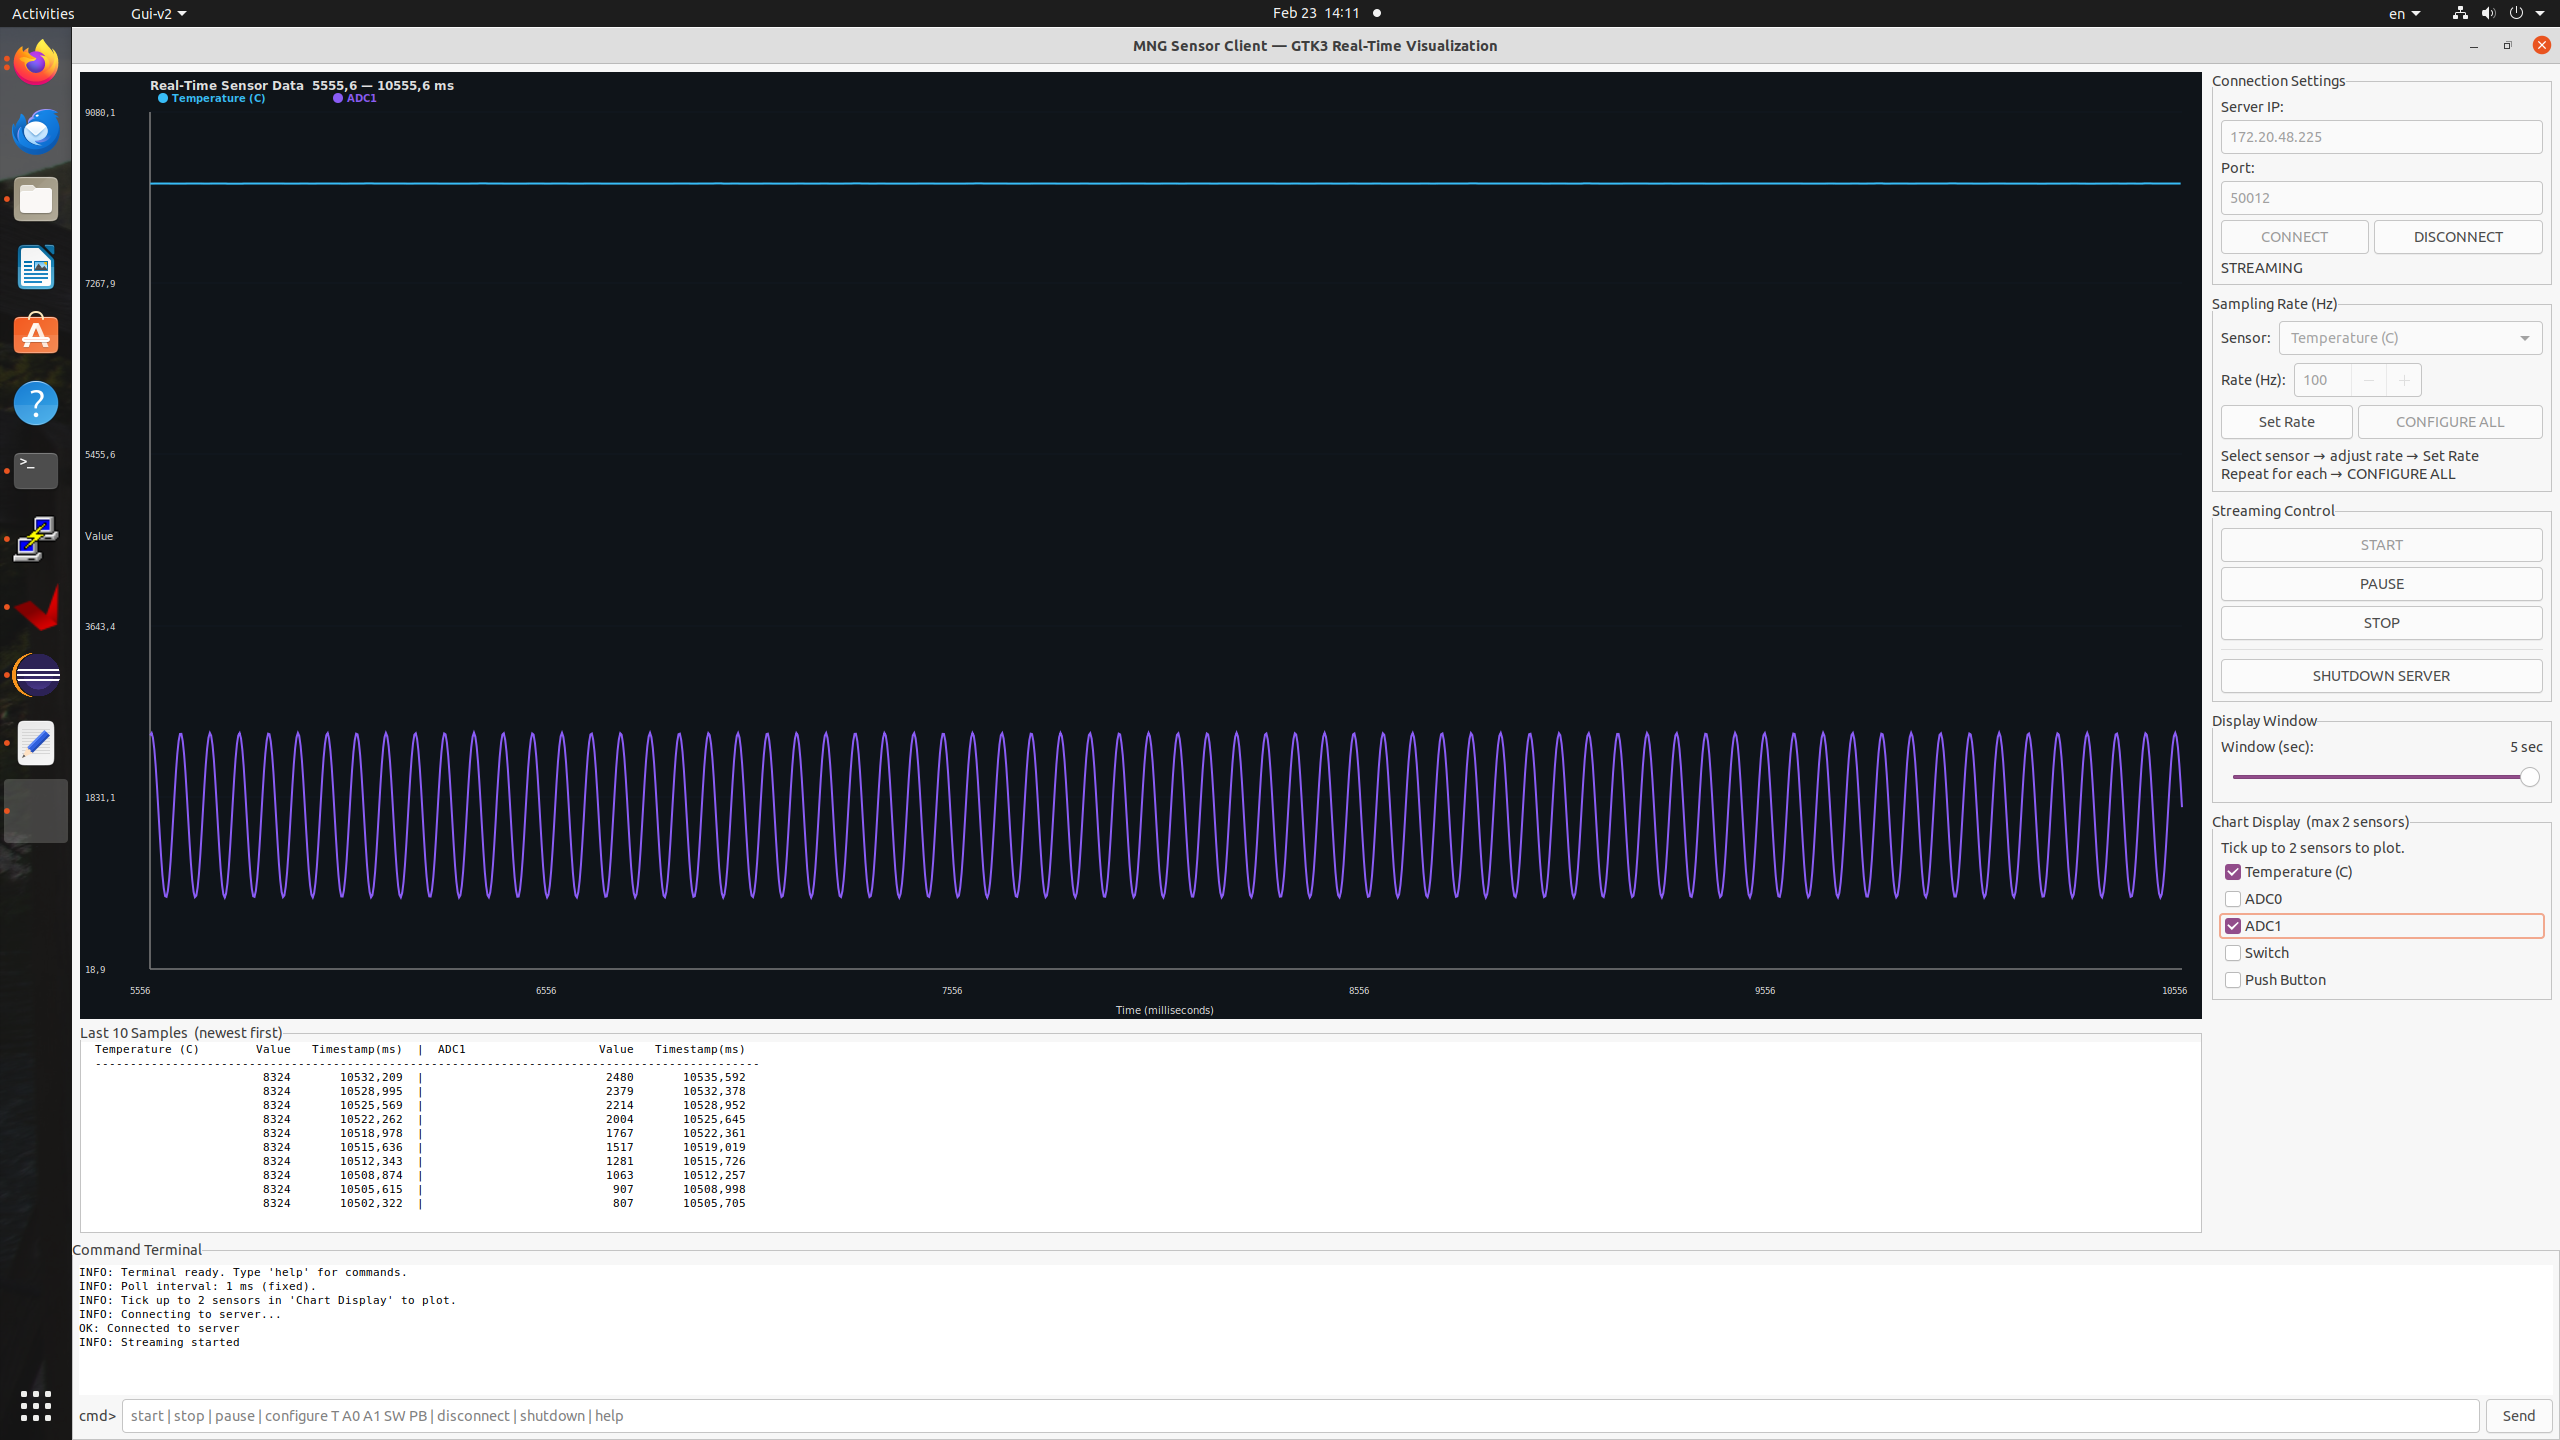
\includegraphics[scale = 0.29]{media/sc3.png}
    \caption{MNG Sensor Client main window overview.}
    \label{fig:gui_overview}
\end{figure}
\end{landscape}
The waveform chart renders up to two sensor signals simultaneously, each
distinguished by a unique colour. The horizontal axis represents elapsed time
in milliseconds, and the vertical axis displays the corresponding raw sensor
values. The visible time window is adjustable through a slider in the control
panel, ranging from 1 to 5 seconds, allowing the user to inspect both
short-term signal behaviour and longer acquisition trends.


\begin{figure}[H]
    \centering
        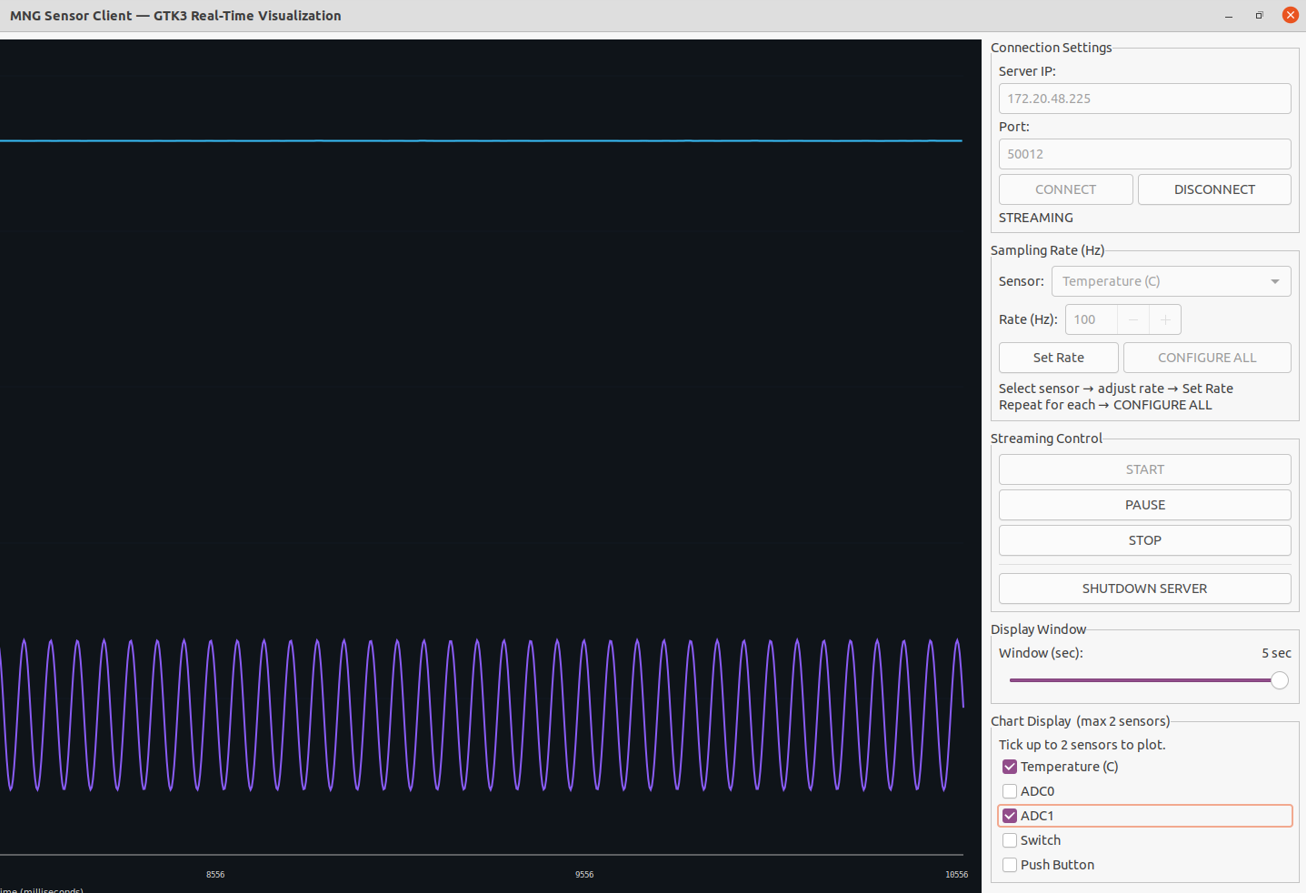
\includegraphics[width=0.8\textwidth]{media/panel_mahdi.png}
        \caption{GUI in active streaming session.}
        \label{fig:gui_streaming}
\end{figure}

\begin{figure}[H]
    \centering
    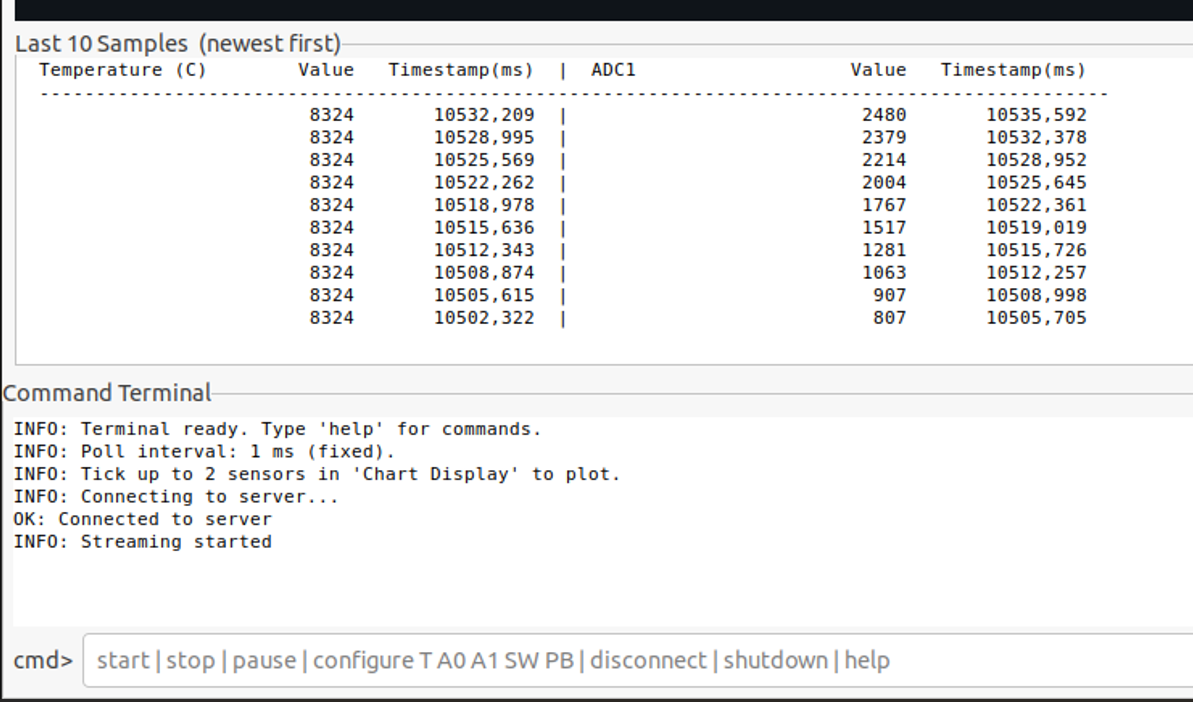
\includegraphics[width=0.8\textwidth]{media/terminal_mahdi.png}
    \caption{Embedded command terminal showing session log}
    \label{fig:gui_terminal}
\end{figure}



As shown in Figure~\ref{fig:gui_streaming}, during an active streaming session
the START button is disabled and the PAUSE and STOP buttons become available,
reflecting the current operational state enforced by the
\texttt{update\_button\_states()} function. The status label at the top of the
control panel updates in real time to indicate the current state, displaying
\texttt{STREAMING}, \texttt{PAUSED}, or \texttt{Connected - Ready} as
appropriate.

The embedded command terminal, shown in Figure~\ref{fig:gui_terminal}, provides
a text-based interface at the bottom of the window through which the user can
issue control commands directly. All session events --- including connection
establishment, configuration changes, streaming state transitions, and error
conditions are logged to the terminal with appropriate prefixes
(\texttt{INFO}, \texttt{OK}, \texttt{WARN}, \texttt{ERROR}), giving the user a
complete chronological record of the session activity.




%\section{UI layout and user Interaction}
%\subsection{Application Context and Initialization}
%\subsection{Callbacks and periodic refresh}




\clearpage 
\null 
\vfill 
\begin{center}
{\large \textbf{Akshay Vastrad (42723)}}
\end{center}
\vfill 
\fancyhead[L]{GTK3 UI Layout and User Interaction (Akshay Vastrad 42723)}
\newpage


\chapter{UI Layout and User Interaction}
 



\section{GTK3 UI Layout and User Interaction}

\subsection{Application Context and Initialization}
The initialization phase of the GTK3 client application is a critical foundational step that establishes the software environment necessary to interface with the remote embedded system. This project presents the design and implementation of a robust Measurement Network Gateway, a high-performance userspace C application deployed on a Xilinx Zynq-7000 SoC (ZedBoard). The remote client features a graphical platform utilized to continuously monitor real-time data streams and dynamically configure the distant sensor devices over the TCP/IP network. To manage this, the graphical application relies on a centralized context structure (often defined as ctx), which holds pointers to all the critical GTK widgets—such as labels, entry fields, buttons, and drawing areas—as well as the underlying data buffers required for Cairo graph rendering.

Initialization begins with the \texttt{create\_gui()} function, which serves as the primary constructor for the user interface. During this phase, the application allocates memory for the complex data structures required to hold incoming telemetry, setting the initial states for minimum and maximum graph values, and clearing the arrays to prevent graphical artifacting. Furthermore, because this client application must safely interact with network sockets, the initialization phase is responsible for setting up the necessary threading primitives, including mutexes, to ensure that the graphical thread does not conflict with the background data-receiving thread. The system architecture employs a concurrent Producer-Consumer model utilizing POSIX threads (pthreads).

The main desktop window is instantiated using gtk\_window\_new(GTK\_WINDOW\_TOPLEVEL). The title is explicitly set to "Measurement Network Gateway - Real-Time Data Monitor" to provide clear context to the user. A default resolution of 1500x950 pixels is enforced via gtk\_window\_set\_default\_size(), ensuring that the dashboard launches with ample screen real estate to render highly detailed, dual-axis Cairo graphs without immediate user resizing. Finally, the window is bound to a fundamental destruction callback (on\_window\_destroy) via g\_signal\_connect, ensuring that when the user closes the application, all associated TCP sockets are gracefully terminated, memory is freed, and the GTK main loop is cleanly exited.


\subsection{Top-level Window and Main Layout}
GTK3 fundamentally differs from absolute-positioning UI frameworks by utilizing a dynamic, responsive "box-packing" model. The top-level window acts as the blank canvas, but it can only contain a single root widget. Therefore, the core of the dashboard's architecture relies on a master vertical box, vbox\_main, instantiated with gtk\_box\_new(GTK\_ORIENTATION\_VERTICAL, 10). This master container acts as the structural spine of the application, stacking all subsequent sub-panels, frames, and operational zones from the top of the window to the bottom.

To create a visually cohesive and intuitive user experience, the interface heavily leverages GtkFrame widgets. These frames draw subtle borders around logically grouped components and provide embedded text headers, such as "Connection", "Sensor Frequency Set(Hz)", and "Sensor Data (Live)". Inside these frames, horizontal boxes (hbox\_conn, hbox\_config) are packed. This allows widgets like the server IP entry (gtk\_entry\_new) and the connection buttons to sit neatly side-by-side in a single row. This layout strategy is entirely responsive; if the user maximizes the application window, the box-packing algorithm automatically redistributes the free space, keeping the control panels anchored and proportioned correctly without distorting the text or buttons.

A pivotal structural component of the main layout is the GtkPaned widget, which splits the lower section of the window horizontally. The gtk\_paned\_new(GTK\_ORIENTATION\_HORIZONTAL) function creates a draggable divider (set to an initial position of 350 pixels via gtk\_paned\_set\_position). This empowers the user to dynamically adjust the visual ratio between the raw numerical statistics on the left and the graphical plotting area on the right. This separation of concerns within the UI mirrors the backend architecture; it cleanly isolates the control logic (top), the raw data readout (left), and the analytical visualization (right), resulting in an industrial-grade dashboard that is highly legible and operationally efficient.


\subsection{Left Side: Drawing Area + Statistics}
The left side of the dashboard's paned layout is dedicated to delivering immediate, raw, and high-precision statistical readouts from the embedded gateway. The primary objective is to acquire high-precision data from a heterogeneous suite of sensors including a MAX31865 RTD-to-Digital converter for temperature, analog inputs (ADC), and digital I/O (switches and push buttons). To present this continuous stream of data cleanly, the left pane utilizes a vertical box (vbox\_sensors) acting as a tabular column.

Each individual sensor is granted its own horizontal row (hbox\_temp, hbox\_adc0, etc.) containing three distinct GtkLabelwidgets. The first label utilizes GTK's markup language (gtk\_label\_set\_markup) to render the sensor's name in bold text, immediately drawing the operator's eye. A fixed width is applied to this title label using gtk\_widget\_set\_size\_request to ensure that all subsequent data labels align perfectly into a uniform, readable column, much like a spreadsheet. The second label in the row is dedicated to displaying the processed numerical value (e.g., the temperature in Celsius or the ADC voltage), while the third label, aligned strictly to the right edge (GTK\_ALIGN\_END), displays the corresponding microsecond timestamp of that specific reading.

While the exact layout code dictates placing the raw statistics on the left and the Cairo GtkDrawingArea on the right side of the paned divider, they function as a unified data presentation layer. The drawing area acts as the visual counterpart to the statistics. It maps the raw timestamps and normalized integer values into a continuous sliding-window graph. By keeping the live numeric labels (statistics) visibly anchored on the left while the complex, CPU-intensive Cairo graphics render the historical trends on the right, the user receives both immediate situational awareness (the current exact temperature) and analytical context (the thermal trend over the last 10 seconds) simultaneously. This fulfills the primary objective of providing a fault-tolerant foundation for real-time remote monitoring


\subsection{Right Side: Scrollable Control Panel}
The control panel components of the UI—distributed across the top frames and the right side of the graph—are responsible for translating user intent into TCP payloads destined for the remote ZedBoard. The dashboard must safely allow remote users to dynamically adjust sampling rates or pause the stream. To achieve this safely, the UI employs highly constrained input widgets. For frequency configuration, GtkSpinButton widgets are utilized (gtk\_spin\_button\_new\_with\_range). By explicitly setting the allowable range from 10Hz to 10,000Hz, the UI mathematically prevents the operator from submitting an invalid polling rate that could crash the embedded kernel driver or overwhelm the network socket.

Each sensor (Temperature, ADC0, ADC1, Switch) features its own independent spin button paired with a dedicated "Set" button. The configure command parses space-delimited string payloads to dynamically update the independent polling frequencies of the ADC, temperature, and switch components on the fly. When a user clicks a "Set" button, the GTK application extracts the double-precision value from the spin button, formats it into the custom "configure" command string, and dispatches it over the network.

Crucially, the control panel implements strict state-management logic to ensure operational safety. Upon application launch, buttons such as "Start", "Stop", "Disconnect", and the various "Set" configuration buttons are deliberately greyed out and disabled using gtk\_widget\_set\_sensitive(widget, FALSE). They only become active once the "Connect" button successfully establishes a valid TCP socket with the server IP address provided in the GtkEntry field. On the right side of the graph, a localized control panel utilizes GtkComboBoxText dropdown menus. These allow the user to instantly select which specific sensor streams are mapped to the red and blue plotting axes of the Cairo drawing area, granting powerful, real-time customization of the data visualization without needing to restart the stream.


\subsection{Bottom: Command Terminal UI}
To provide deep diagnostic visibility into the network communication between the PC client and the embedded Linux gateway, the bottom of the dashboard layout features a dedicated command terminal UI. In complex industrial deployments, simply seeing a graph is often insufficient for debugging connection drops, packet corruption, or hardware fault flags originating from the remote sensors. The terminal acts as a transparent window into the underlying TCP/IP protocol, providing the operator with a raw, chronological feed of system events and data payloads.

This terminal is constructed using a GtkTextView widget embedded within a GtkScrolledWindow. The scrolled window is explicitly configured to handle vertical overflow, meaning that as thousands of lines of log data are generated, the view automatically provides a scrollbar rather than allowing the UI layout to expand off the physical screen. The text view itself is bound to a GtkTextBuffer, which holds the actual string data. To ensure the terminal acts purely as a diagnostic log and not an accidental input field, the widget is strictly locked using gtk\_text\_view\_set\_editable(FALSE).

As the background networking thread receives TCP packets, it unpacks the custom command protocol. If the client software evaluates the least significant bit (Bit 0) and detects a hardware fault flag, or if the connection status changes, these events are appended to the text buffer. A utility function is utilized to automatically move the text cursor (GtkTextIter) to the very end of the buffer after every insertion, forcing the scrolled window to automatically scroll down. This ensures the user is always looking at the absolute latest network event, creating a highly effective, live-scrolling diagnostic terminal that complements the graphical plotting area above it.


\subsection{Callbacks and Periodic Refresh}
The GTK3 framework relies on an event-driven architecture, meaning the application idles in a main loop (gtk\_main()) until an internal timer fires or a user interacts with a widget. This interaction is handled entirely through callbacks and signal routing. Every interactive widget in the dashboard is mapped to a specific C function using g\_signal\_connect. For example, clicking the "Connect" button triggers the on\_connect\_clicked callback, which immediately attempts to open a non-blocking TCP socket to the IP address specified in the UI.

Because the GTK main loop must never be blocked (otherwise the UI will freeze and the application will become unresponsive to the OS), the continuous rendering of the Cairo graph is managed via a periodic refresh timer. A function such as g\_timeout\_add() is initialized to fire every ~33 milliseconds (yielding approximately 30 frames per second). When this timer ticks, it triggers a callback that updates the numerical GtkLabel statistics and issues a gtk\_widget\_queue\_draw() command to the GtkDrawingArea. This queues an expose event, forcing GTK to invoke the on\_draw\_graph function, which subsequently recalculates the sliding time window and redraws the grid, axes, and sensor lines.

Thread synchronization is paramount within these callbacks. The background networking thread is constantly listening to the TCP socket and pushing new data points into the client-side buffers. Since the GTK UI thread and the networking thread run concurrently, accessing the graph data arrays simultaneously would cause fatal race conditions or corrupted screen renders. Therefore, whenever the on\_draw\_graph callback is fired by the refresh timer, it first executes a pthread\_mutex\_lock() on the shared context structure. It reads the historical data, plots the pixels, and then immediately calls pthread\_mutex\_unlock(). This guarantees atomic access to the data, ensuring a perfectly smooth, tear-free graphical user experience.


\clearpage
\null
\vfill 
\begin{center}
{\large  \textbf{Mohammad Raza Rahimi (42756)}} \\     
\end{center}
\vfill 
\fancyhead[L]{Data Buffering, Time window, Plotting in GUI (Mohammad Reza Rahimi 42756)}
\clearpage 

\chapter{Client Side Data Buffering, Statistic and Plotting}


\subsection{Client Side Data Buffering, Statistics, and Real Time Plotting}
First the ring buffer collects sensor samples from the sensor thread and then delivers them to the server thread. On the GUI (client) side, a similar mechanism is needed: incoming samples must be stored, organized per sensor, and then used for plotting and statistics. This section explains all data structures and functions responsible for this task.

\subsubsection{Incoming Data - The Network Packet}
Every sample that arrives over TCP is a packed structure called net\_packet\_t:
    \begin{minted}[bgcolor = lightgray, tabsize = 4, breaklines ]{c}
    typedef struct __attribute__((packed)) {
        int32_t sid;      /* sensor ID: 1=Temp, 2=ADC0, 3=ADC1, 4=Switch, 5=PushBtn */
        int32_t svalue;   /* raw sensor value (integer) */
        int64_t ts;       /* timestamp in microseconds from server start */
    } net_packet_t;
\end{minted}

This structure is exactly 16 bytes because this \texttt{\_attribute\_((packed))} directive that it removes any padding between fields. With identifying which sensor produces sample by \texttt{sid} filed, then the \texttt{svalue} holds raw measurement and \texttt{ts} is the timestamp in microseconds assigned by the server's \texttt{GetElapsedTime()} function.

Network thread receives the raw bytes from the TCP socket and it is going to check whether at least \texttt{sizeof(net\_packet\_t)} bytes are available, then it is going to extracts one packet and calls buffer\_add\_sample(pkt.sid, pkt.svalue, pkt.ts) to store the sample in the correct per sensor buffer.

\begin{minted}[bgcolor = lightgray, tabsize = 4, breaklines]{c}
	typedef struct {
    double   values[MAX_SAMPLES];    /* sensor values (converted to double) */
    int64_t  ts_us[MAX_SAMPLES];     /* timestamps in microseconds */
    int      count;                  /* number of stored samples */
    int      oldest_idx;             /* index of oldest sample (when full) */
    int64_t  start_time_us;          /* timestamp of the very first sample */
    pthread_mutex_t lock;            /* protects concurrent access */
	} sensor_buffer_t;
\end{minted}
The constant \texttt{MAX\_SAMPLES} is set to 2000 that means each sensor can only store up to 2000 data points before older values are overwritten. Thers is \texttt{count} filed which is showing  how many samples have been added so far. As long as count < MAX\_SAMPLES, new samples are appended at index count. Once the \texttt{count == MAX\_SAMPLES}, the buffer becomes circular it means buffer is full: new samples overwrite the entry at oldest\_idx, which is then incremented modulo the buffer size.
The start\_time\_us field stores the timestamp of the first sample for that sensor and all the other which is coming later subsequent timestamps are plotted relative to this value, so the x-axis starts near zero.
The pthread\_mutex\_t responsible for lock ensures thread safety. Since the network thread (calling buffer\_add\_sample) and the GTK main thread (calling buffer\_get\_copy and buffer\_stats) run concurrently, the mutex is trying to avoid simultaneous access to the buffer.

\begin{minted}[bgcolor = lightgray, tabsize = 4, breaklines]{c}
sensor_buffer_t buf[MAX_SENSORS + 1];   /* buf[1]..buf[5], index 0 unused */
\end{minted}

\begin{figure}[H]
\centering 
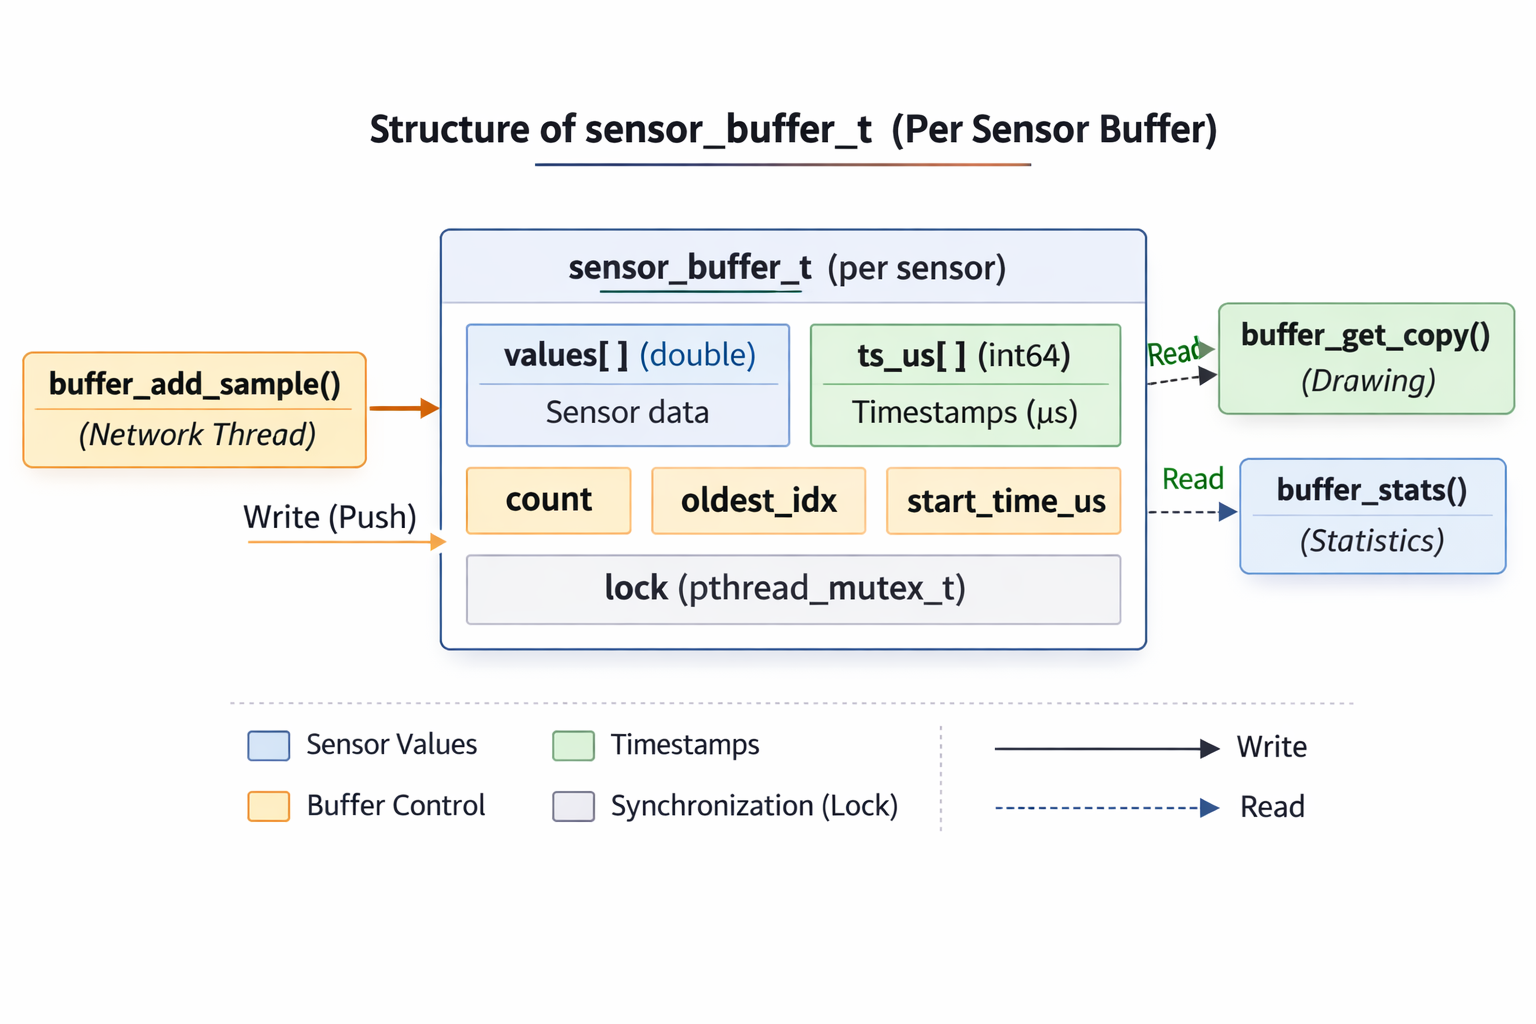
\includegraphics[width = 0.9\textwidth, trim = 0cm 2cm 0cm 0cm, clip]{media/imageRezaGUI1.png}
\caption{Structure of sensor\_buffer\_t}
\label{fig-guireza1}
\end{figure}

\subsubsection{Buffer Initialization \texttt{buffer\_init}}
\begin{minted}[bgcolor = lightgray, tabsize = 4, breaklines]{c}
static void buffer_init(int sid) {
    if (sid < 1 || sid > MAX_SENSORS) return;
    sensor_buffer_t *b = &g_app.buf[sid];
    pthread_mutex_init(&b->lock, NULL);
    b->count = 0;
    b->oldest_idx = 0;
    b->start_time_us = 0;
}
\end{minted}
This function is called once for each sensor (sid = 1 to 5) during the GUI startup in build\_ui(). It initializes the POSIX mutex and sets count, oldest\_idx, and start\_time\_us to zero, which means the buffer starts empty and ready to receive samples.

\subsubsection{Adding a sample \texttt{buffer\_add\_sample}}
\begin{minted}[bgcolor = lightgray, tabsize = 4, breaklines]{c}
static void buffer_add_sample(int sid, int value, int64_t ts_us) {
    if (sid < 1 || sid > MAX_SENSORS) return;
    sensor_buffer_t *b = &g_app.buf[sid];
    pthread_mutex_lock(&b->lock);

    if (b->count == 0) b->start_time_us = ts_us;
    if (ts_us > g_app.last_data_time_us)
        g_app.last_data_time_us = ts_us;

    if (b->count < MAX_SAMPLES) {
        int idx = b->count++;
        b->values[idx] = (double)value;
        b->ts_us[idx]  = ts_us;
    } else {
        int idx = b->oldest_idx;
        b->values[idx] = (double)value;
        b->ts_us[idx]  = ts_us;
        b->oldest_idx  = (b->oldest_idx + 1) % MAX_SAMPLES;
    }

    pthread_mutex_unlock(&b->lock);
}
\end{minted}
This function is the producer of the client side buffer; it is called by the network thread every time a net\_packet\_t is successfully extracted from the TCP stream.

Step by step: 
\begin{enumerate}
\item	Guard check: if sid is out of range (not 1–5), the function returns immediately.
\item	Lock the mutex: prevents the drawing thread from reading the buffer at the same time.
\item	First sample handling: if this is the very first sample (count == 0), the timestamp is saved as start\_time\_us. This becomes the reference point (time zero) for the x axis.
\item	Global timestamp tracking: last\_data\_time\_us is updated to the newest timestamp across all sensors, which is later used to determine the right edge of the time window in the chart.
\item	Buffer not yet full (count < MAX\_SAMPLES): the sample can still to be written at position count, and then count is incremented.
\item	Buffer full (count == MAX\_SAMPLES): the sample will overwrites the oldest entry at oldest\_idx, and oldest\_idx is going to advance by one with wrap around (\% MAX\_SAMPLES). This is the same circular buffer principle as the server ring buffer.
\item	Unlock the mutex.
\end{enumerate}

\subsubsection{Reading Samples for Plotting - buffer\_get\_copy}
\begin{minted}[bgcolor = lightgray, tabsize = 4, breaklines]{c}
static int buffer_get_copy(int sid, double *x_ms, double *y, int max_len) {
    if (sid < 1 || sid > MAX_SENSORS) return 0;
    sensor_buffer_t *b = &g_app.buf[sid];
    pthread_mutex_lock(&b->lock);

    if (b->count == 0) { pthread_mutex_unlock(&b->lock); return 0; }
    int n = (b->count < max_len) ? b->count : max_len;

    if (b->count < MAX_SAMPLES) {
        for (int i = 0; i < n; ++i) {
            x_ms[i] = (double)(b->ts_us[i] - b->start_time_us) / 1000.0;
            y[i]    = b->values[i];
        }
    } else {
        for (int i = 0; i < n; ++i) {
            int idx = (b->oldest_idx + i) % MAX_SAMPLES;
            x_ms[i] = (double)(b->ts_us[idx] - b->start_time_us) / 1000.0;
            y[i]    = b->values[idx];
        }
    }

    pthread_mutex_unlock(&b->lock);
    return n;
}
\end{minted}

This is the consumer of the client side buffer; it is called by the drawing function every time the chart needs to be redrawn.
Key points:
\begin{enumerate}
\item It locks the mutex, copies the data into the caller's arrays (x\_ms and y), and unlocks immediately, this minimizes the time the mutex is held, keeping the network thread responsive.
\item Timestamp conversion: the raw microsecond timestamps are converted to milliseconds relative to start\_time\_us using (ts\_us[i] - start\_time\_us) / 1000.0. It shows that the x-axis of chart always start from near zero.
\item Buffer not full (count < MAX\_SAMPLES): data is stored sequentially starting from index 0, so the loop reads indices 0 to n−1 directly.
\item Buffer full: data is read starting from oldest\_idx (the oldest sample), wrapping around with modulo. This guarantees that output should always in somehow order which from oldest to newest.
\item The function returns n, the number of copied samples.
\end{enumerate}


\subsubsection{Computing Statistics - \texttt{buffer\_stats}}
\begin{minted}[bgcolor = lightgray, tabsize = 4, breaklines]{c}
static int buffer_stats(int sid, double *minv, double *maxv,
                        double *avg, int *count) {
    if (sid < 1 || sid > MAX_SENSORS) return 0;
    sensor_buffer_t *b = &g_app.buf[sid];
    pthread_mutex_lock(&b->lock);

    if (b->count == 0) { pthread_mutex_unlock(&b->lock); return 0; }
    double mn = b->values[0], mx = b->values[0], sum = 0.0;
    for (int i = 0; i < b->count; ++i) {
        double v = b->values[i];
        if (v < mn) mn = v;
        if (v > mx) mx = v;
        sum += v;
    }
    *minv = mn;  *maxv = mx;
    *avg  = sum / b->count;
    *count = b->count;

    pthread_mutex_unlock(&b->lock);
    return 1;
}
\end{minted}
This function is computing the minimum, maximum, and average of all stored samples which are for a given sensor. It is called by \texttt{update\_stats\_box()} every 50 ms (the GUI refresh interval). The result is displayed as a formatted line in the ‘Statistics’ panel below the chart. For example:
\begin{center}
\begin{minted}[bgcolor = lightgray, tabsize = 4, breaklines]{text}
SID 1 Temperature (°C) | Min: 23.5 Max: 26.1 Avg: 24.8 (n=1500)
\end{minted}
\end{center}

The function trying to process all stored values in a single pass, then tracking the running minimum, maximum, and sum. Dividing the sum by count yields the arithmetic mean. If the buffer is empty, the function returns 0 and the sensor is omitted from the statistics display.

\subsubsection{Displaying Statistics - \texttt{update\_stats\_box}}
The function \texttt{update\_stats\_box()} is called periodically by the GUI refresh
timer. It performs two steps:

\begin{enumerate}
    \item \textbf{Clear old labels:} It is responsible to remove all child widgets
    from \texttt{g\_app.stats\_box} (the vertical box inside the Statistics frame),
    and trying to prevent the panel from accumulating outdated entries.

    \item \textbf{Rebuild for each active sensor:} For every sensor where
    \texttt{sensor\_enabled[sid]} is true, it calls \texttt{buffer\_stats()} to get
    the current min, max, average, and count, it formats the result into a line using
    \texttt{snprintf}, and then it creates a new GTK label with monospace markup, and
    adds it to the stats box.
\end{enumerate}

This approach rebuilds the statistics display from scratch every refresh cycle, which
is simple and avoids the need to track individual label widgets per sensor.

\subsubsection{Real Time Chart - \texttt{on\_draw\_chart}}
The \texttt{on\_draw\_chart()} function is the Cairo drawing callback which is connected
to the \texttt{GtkDrawingArea}. GTK calls it automatically whenever
\texttt{gtk\_widget\_queue\_draw()} is triggered, which occurs every 50\,ms via the
\texttt{ui\_update\_cb} timer.

The drawing process has five stages:

\begin{enumerate}
    \item \textbf{Stage 1-Background and grid:} The function clears the drawing area
    which is using a dark background color (\texttt{rgb(0.06, 0.08, 0.10)}) and it is
    going to draws five horizontal grid lines plus the X and Y axes in gray.

    \item \textbf{Stage 2-Determine data range:} A first loop iterates over all enabled
    sensors, calls \texttt{buffer\_get\_copy()} for each, and then it scans the returned
    values to determine the global minimum and maximum for both the time (x-axis) and
    value (y-axis). If there is no sensor has data, the function displays
    ``Waiting for data\ldots'' and returns.

    \item \textbf{Stage 3-Time window and y-axis scaling:} The user-selected time window
    (\texttt{time\_range\_seconds}, e.g., 5 seconds = 5000\,ms) which it defines the
    visible data range. The right edge of the window (\texttt{t\_max}) is set to the
    latest timestamp, and the left edge (\texttt{t\_min}) is
    \texttt{t\_max}~\(-\)~\texttt{time\_window\_ms}. A 10\% padding is added above and
    below the y-range so curves do not touch the borders.

    \item \textbf{Stage 4-Draw sensor curves:} A second loop iterates over all enabled
    sensors again. For each sensor, \texttt{buffer\_get\_copy()} provides the
    (time, value) arrays. Each sensor has a unique color defined in the
    \texttt{g\_sensors} table (e.g.\ temperature = light blue, ADC0 = red). The code
    maps each data point from data coordinates to pixel coordinates using:
    
    \begin{minted}[bgcolor = lightgray, tabsize = 4, breaklines]{text}
pixel_x = margin_left + ((time_ms - t_min) / t_range) * plot_width
pixel_y = margin_top + plot_height - ((value - y_min) / y_range) * plot_height
\end{minted}

Points outside the time window are skipped, and the curve is drawn as a polyline using cairo\_move\_to(), cairo\_line\_to(), and cairo\_stroke().

\item \textbf{Stage 5-Axis labels and title:} The y-axis shows six evenly spaced value ticks, the x-axis shows six evenly spaced time ticks (in milliseconds), and a title at the top displays the current time window (for example, “Real-Time Sensor Data - 1200.0 to 6200.0 ms”).
\end{enumerate}



\begin{figure}[H]
\centering 
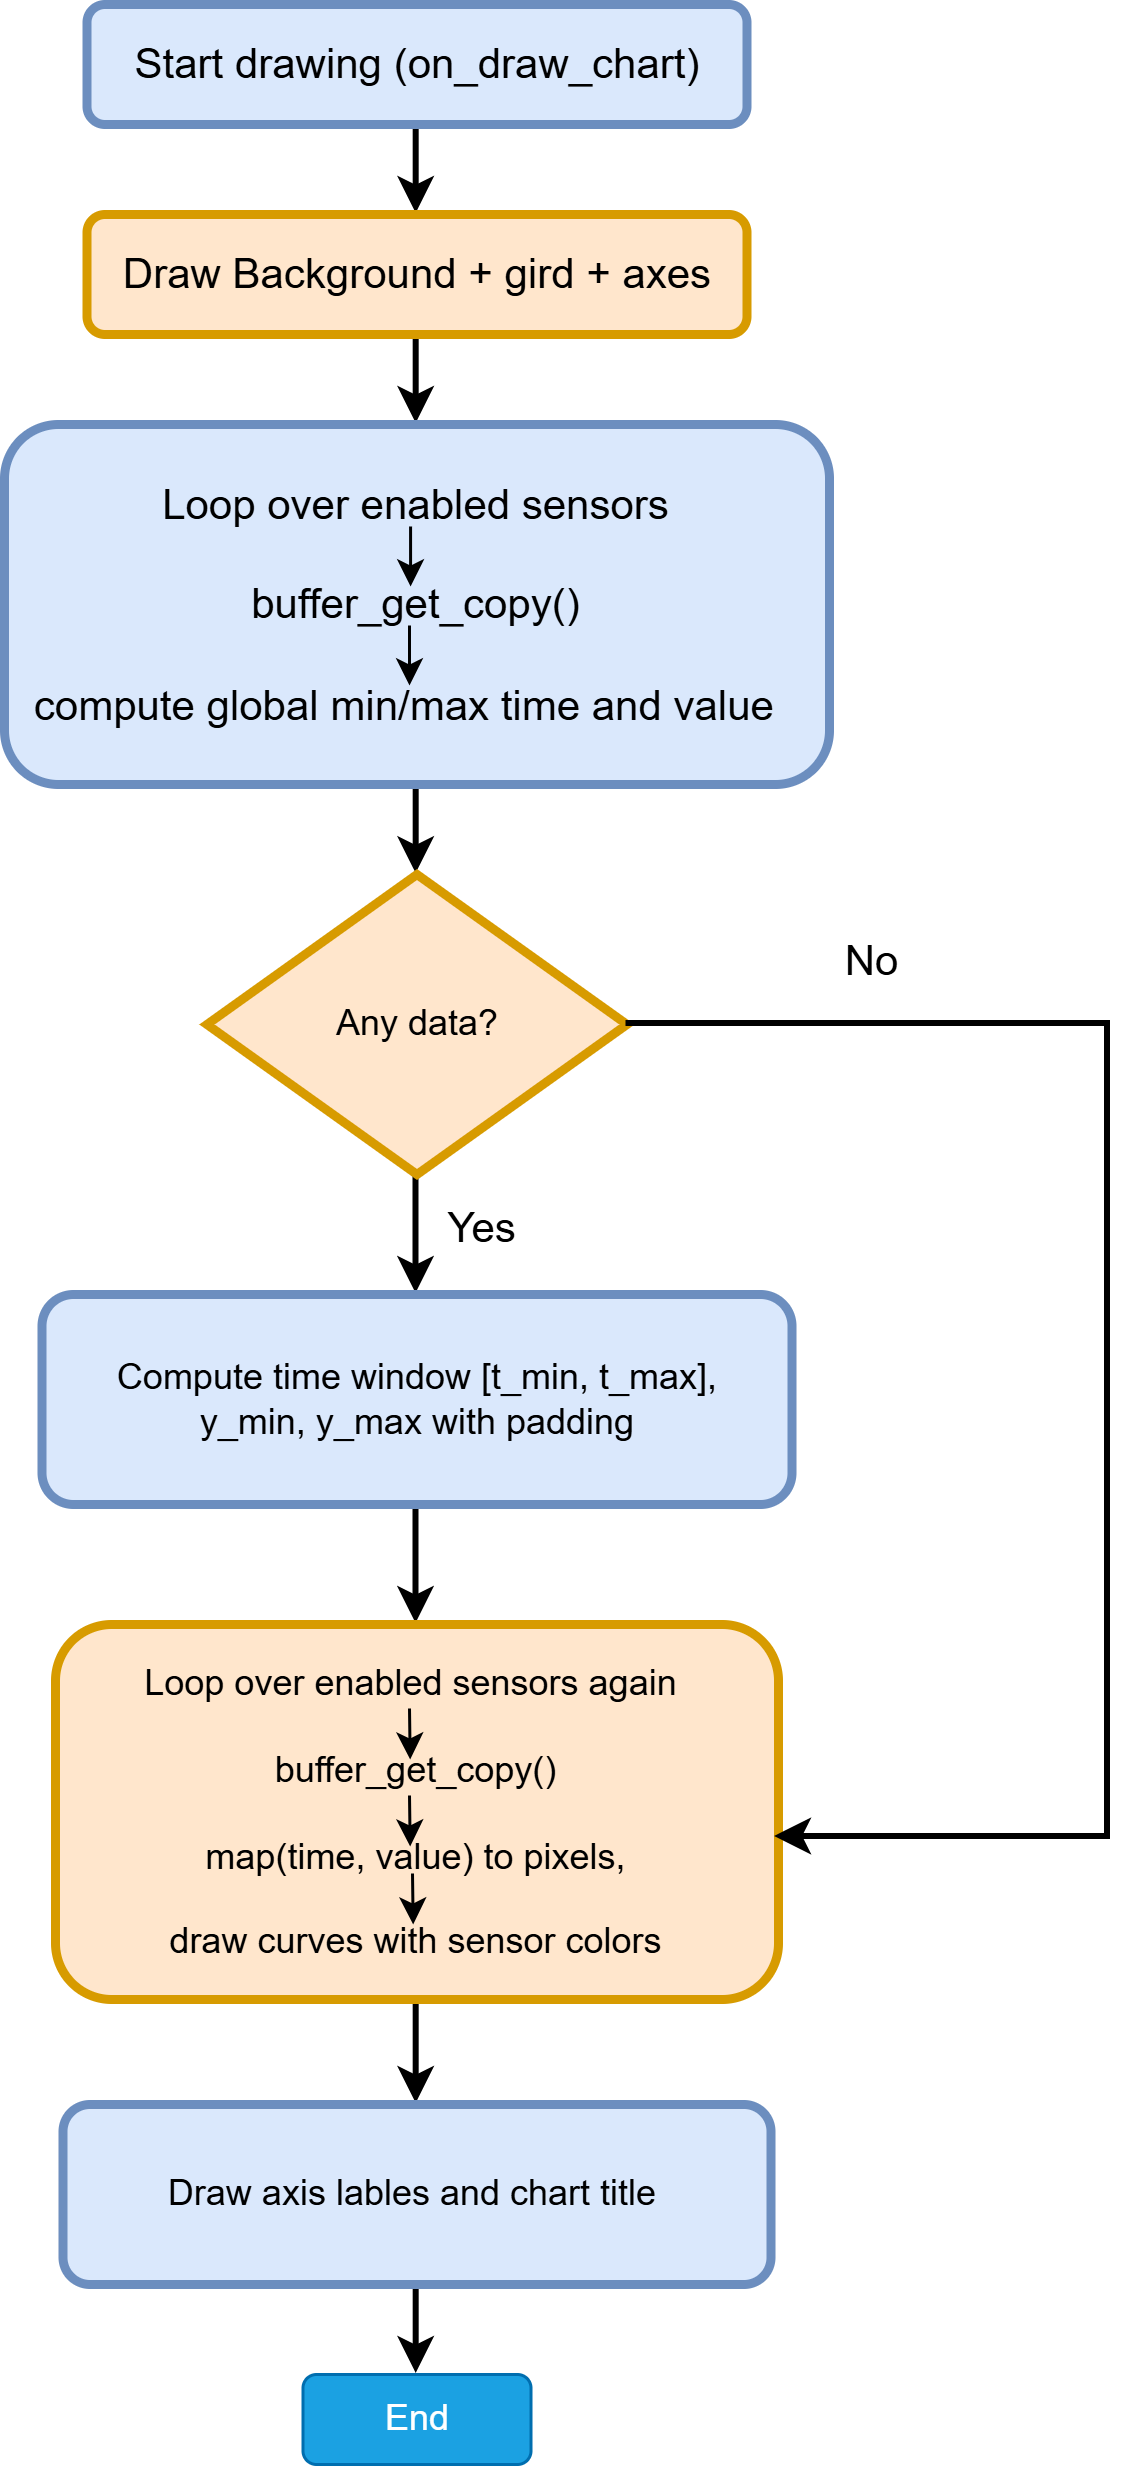
\includegraphics[scale = 0.8]{media/imageRezaGUI2.png}
\caption{Drawing pipeline inside \texttt{on\_draw\_chart()}}
\label{fig-rezagui2}
\end{figure}

\subsubsection{Sensor Visibility and Time Window Control}
Two user controls directly affect the chart and statistics:

\begin{itemize}
    \item \textbf{Visible Sensors checkboxes:} each sensor has a \texttt{GtkCheckButton}.
    When the user toggles it, the \texttt{on\_sensor\_toggled()} callback sets
    \texttt{g\_app.sensor\_enabled[sid]} to true or false and triggers a redraw. Just
    the enabled sensors are included in the global min/max calculation, plotting, and
    statistics panel display.

    \item \textbf{Display Window slider:} A horizontal \texttt{GtkScale} lets the user
    select how many seconds of data are visible (1 to 5 seconds). 
\end{itemize}
The \texttt{on\_time\_range\_changed()} callback updates \texttt{g\_app.time\_range\_seconds} and also the label text (for example, ‘5 sec’), then it triggers a redraw. With a larger window shows more history but there will be less detail. So a smaller window zooms in on the latest samples.

\subsubsection{Periodic Refresh - \texttt{ui\_update\_cb}}
\begin{minted}[bgcolor = lightgray, tabsize = 4, breaklines]{c}
static gboolean ui_update_cb(gpointer data) {
    if (g_app.should_close) return FALSE;
    /* update status label based on connection state */
    gtk_widget_queue_draw(g_app.drawing_area);
    update_stats_box();
    return TRUE;
}
\end{minted}
This timer callback is registered once in main() with a period of UPDATE\_INTERVAL\_MS = 50 ms, meaning the chart and statistics refresh at approximately 20 frames per second. It calls \texttt{gtk\_widget\_queue\_draw()}, which tells GTK to invoke \texttt{on\_draw\_chart()} on the next main loop iteration, and \texttt{update\_stats\_box()} to rebuild the statistics panel. Returning \texttt{TRUE} keeps the timer repeating; returning \texttt{FALSE} (when the window is closing) stops it.

\subsubsection{Connection to the Server Side Ring Buffer}
This client-side buffering is the second stage of the overall data pipeline in the
Measurement Network Gateway:

\begin{itemize}
    \item \textbf{Server ring buffer (your ring buffer chapter):} the sensor thread
    pushes timestamped (\texttt{sid}, \texttt{ts}, \texttt{svalue}) entries; the server
    thread pops them and packs them into TCP packets.

    \item \textbf{TCP transport:} packets travel from the server to the GUI client as
    raw \texttt{net\_packet\_t} bytes.

    \item \textbf{Client per-sensor buffers (this section):} incoming packets are sorted
    by \texttt{sid} into five separate circular buffers, converted to doubles, and made
    available for plotting and statistics.
\end{itemize}

The server ring buffer holds all five sensors mixed together in a single FIFO queue,
while the client separates them into individual buffers so each sensor can be plotted
and analyzed independently.

\begin{figure}[H]
\centering 
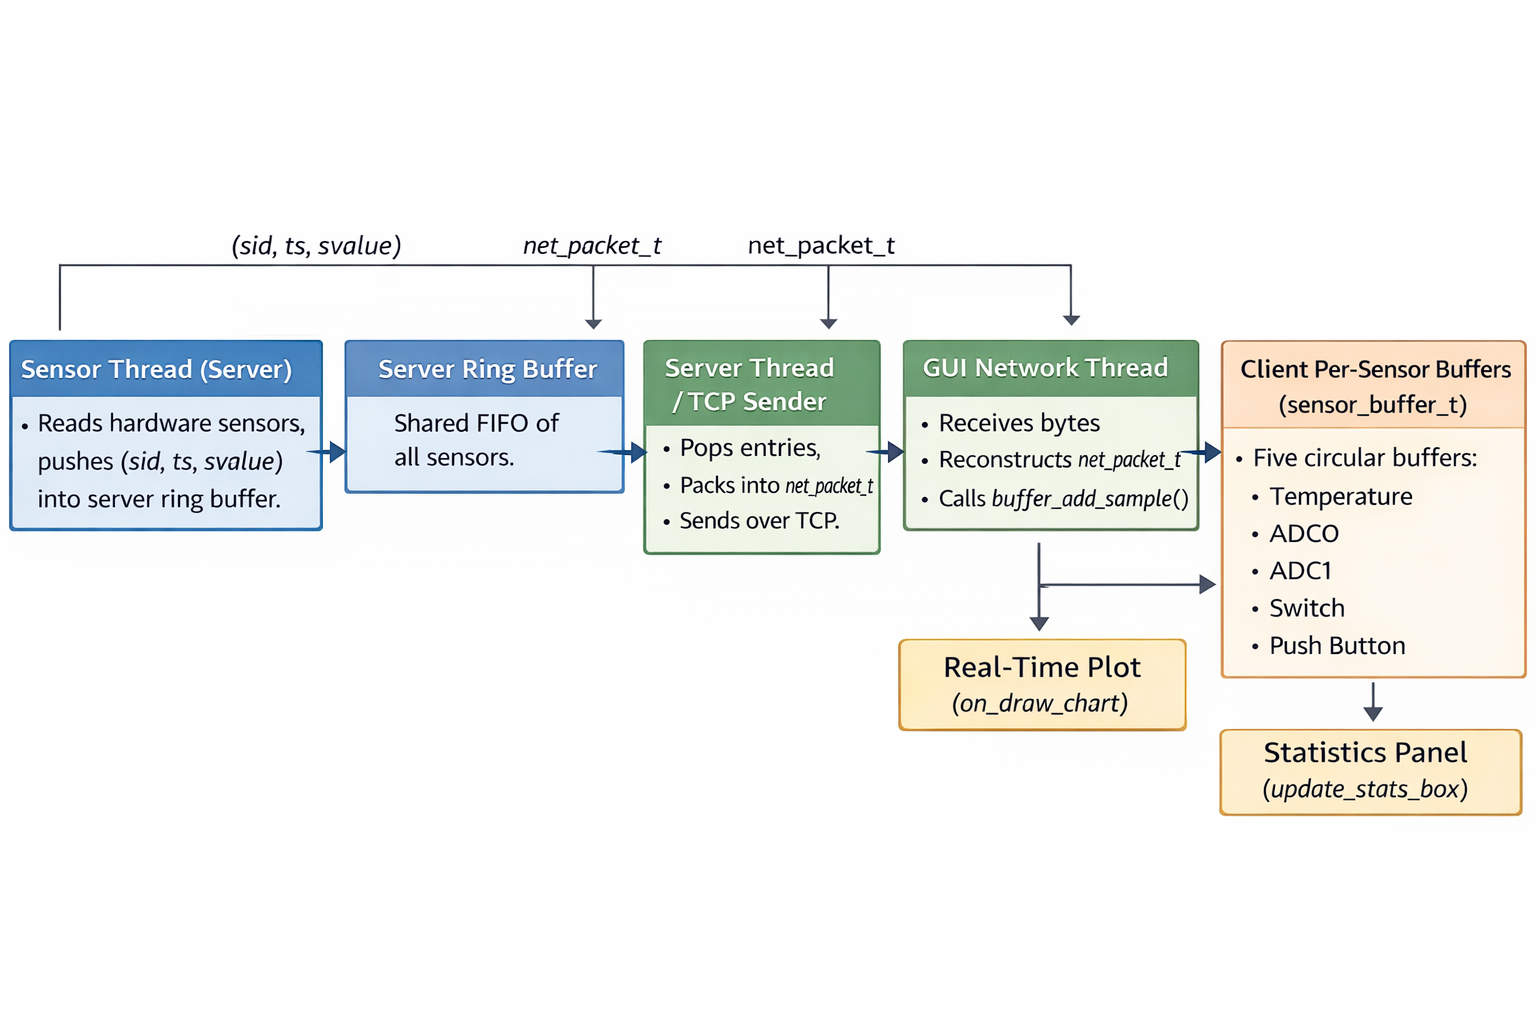
\includegraphics[width = 0.85\textwidth]{media/imageRezaGUI3.png}
\caption{Data flow from server ring buffer to GUI buffers}
\label{fig-rezagui3}
\end{figure}



\section{Requirement Compliance and Verification}
This section discusses the compliance of requirements for the application and GUI built by Mohammad Mahdi Mohammadi, Mohammad Reza Rahimi and Akshay Vastrad. 
\subsection{Compliance Summary}
The Measurement Network Gateway system has been developed and verified against a total of 24 specified requirements covering Functional, Design, RAMS, and Test categories.
\begin{table}[h!]
    \centering
    \caption{Requirements Compliance Summary}
    \begin{tabular}{|l|c|c|}
        \hline
        \textbf{Category} & \textbf{Total Requirements} & \textbf{Implemented}\\
        \hline
        Functional & 12 & 12 \\
        Design     & 5  & 5  \\
        RAMS       & 4  & 4  \\
        Test       & 3  & 3  \\
        \hline
        \textbf{TOTAL} & \textbf{24} & \textbf{24} \\
        \hline
    \end{tabular}
    \label{tab:requirements_compliance}
\end{table}

All 24 system requirements have been fully implemented and verified. No open compliance gaps remain.



\subsection{Requirements Traceability Matrix}

\begin{table}[h!]
    \centering
    \label{tab:req_traceability}
    \small
    \begin{tabularx}{\linewidth}{|l|X|X|l|}
        \hline
        \textbf{Req ID} & \textbf{Requirement Description} & \textbf{Technical Implementation} & \textbf{Verification Method} \\
        \hline
        REQ-1  & Multi-sensor TCP gateway              & Sensor + Server threads, Ring Buffer, TCP port 50012          & Integration test         \\
        \hline
        REQ-2  & Precision RTD temperature acquisition & PT100 + MAX31865, \texttt{TempRead()}, \texttt{sid\_temp}     & Sensor validation test   \\
        \hline
        REQ-3  & Dual ADC signal capture               & PmodAD1 (ADC0/ADC1), \texttt{GetADC()}, \texttt{sid\_adc0/1} & Signal injection test    \\
        \hline
        REQ-4  & Digital switch acquisition            & ZedBoard 8-bit DIP, \texttt{ReadSwitch()}                     & Functional test          \\
        \hline
        REQ-5  & Pushbutton acquisition                & ZedBoard 5 buttons, \texttt{ReadButton()}                     & Functional test          \\
        \hline
        REQ-6  & Configurable sampling rates           & Per-sensor Hz config, \texttt{period\_us = 1M/Hz}             & Timing verification      \\
        \hline
        REQ-7  & Selectable sensor activation          & Rate=0 disables sensor, conditional sampling                  & Configuration test       \\
        \hline
        REQ-8  & Timestamped measurements              & \texttt{CLOCK\_MONOTONIC}, 1\,\textmu s resolution            & Time accuracy validation \\
        \hline
        REQ-9  & GUI sensor configuration              & GTK configuration panel                                       & GUI validation           \\
        \hline
        REQ-10 & GUI sampling rate configuration       & Per-sensor Hz input fields                                    & GUI validation           \\
        \hline
        REQ-11 & GUI text data display                 & Live table with real-time updates                             & Runtime test             \\
        \hline
        REQ-12 & GUI dual-signal plotting              & Cairo-based dual-channel charts                               & Visual verification      \\
        \hline
    \end{tabularx}
    \caption{Functional Requirements (REQ-1 \rightarrow REQ-12)}
\end{table}


\begin{table}[h!]
    \centering
    \label{tab:design_traceability}
    \small
    \begin{tabularx}{\linewidth}{|l|X|X|l|}
        \hline
        \textbf{Req ID} & \textbf{Requirement} & \textbf{Implementation} & \textbf{Verification} \\
        \hline
        REQ-13 & Embedded Linux platform       & Zynq-7000 ZedBoard, ARM Cortex-A9, PetaLinux        & Platform validation  \\
        \hline
        REQ-14 & Multithreaded architecture    & Two POSIX threads with mutex synchronization         & Concurrency test     \\
        \hline
        REQ-15 & GTK-based GUI application     & GTK+3.0, GLib event loop                            & GUI validation       \\
        \hline
        REQ-16 & Binary data protocol          & 16-byte packet structure                            & Protocol inspection  \\
        \hline
        REQ-17 & TCP payload $\leq$ 1500 bytes & $93 \times 16$B packets $= 1488$ bytes               & Network measurement  \\
        \hline
    \end{tabularx}
    \caption{Design Requirements (REQ-13 \rightarrow REQ-17)}
\end{table}




\begin{table}[H]
    \centering
    \label{tab:rams_traceability}
    \small
    \begin{tabularx}{\linewidth}{|l|X|X|l|}
        \hline
        \textbf{Req ID} & \textbf{Requirement} & \textbf{Implementation} & \textbf{Verification} \\
        \hline
        REQ-18 & Controlled startup and shutdown & Thread creation/join, graceful termination                                          & Lifecycle test      \\
        \hline
        REQ-19 & Resource initialization         & \texttt{InitTimer()}, \texttt{InitRingBuffer()}, \texttt{TempPowerUp()}              & Code inspection     \\
        \hline
        REQ-20 & Sensor power-down handling      & \texttt{TempShutdown()} disables MAX31865 VBIAS                                     & Hardware validation \\
        \hline
        REQ-21 & Resource cleanup                & Mutex destroy, socket close, thread join                                            & Shutdown validation \\
        \hline
    \end{tabularx}
    \caption{RAMS Requirements (REQ-18 to REQ-21)}
\end{table}


\begin{table}[h!]
    \centering
    \label{tab:test_traceability}
    \small
    \begin{tabularx}{\linewidth}{|l|X|X|l|}
        \hline
        \textbf{Req ID} & \textbf{Requirement} & \textbf{Implementation} & \textbf{Verification} \\
        \hline
        REQ-22 & Auxiliary digital test inputs      & Switches/buttons used as test signals          & Hardware validation   \\
        \hline
        REQ-23 & Functional testing capability      & Simulation mode with synthetic data            & Mode comparison test  \\
        \hline
        REQ-24 & Timing performance evaluation      & Microsecond timestamps, jitter logging         & Timing analysis       \\
        \hline
    \end{tabularx}
    \caption{Test Requirements (REQ-22 to REQ-24)}
\end{table}







%======================================================================================

\newpage
\null 
\vfill
\begin{center}
\textbf{\large Mert Ali Türk (42746)}
\end{center}
\vfill
\fancyhead[L]{MNG Software Development (Mert Ali Türk 42746)}
\clearpage

\chapter{MNG Software Development}
\section{Software Development(Mert Ali Turk)}

\subsection{Introduction to Software Development}
The application software for the Measurement Network Gateway runs on the Linux operating 
system. The purpose of the software is to gather sensor values from connected sensors 
and transmit them via the TCP/IP stack. Since the application runs on Linux, POSIX APIs 
are used, particularly for networking functionality.

This is one of the key benefits of using Embedded Linux, as it enables rapid prototyping 
without the need to implement the entire communication stack from scratch. Additionally, 
the Linux image is created using PetaLinux, a Xilinx tool used to generate customized 
Linux images for Zynq devices.

Gathering sensor values also requires access to hardware, since a custom IP core 
is implemented to sample the sensors. In the Linux operating system, hardware access 
is performed through file operations. Therefore, a Linux Kernel Module (LKM) must be 
developed so that the device can be recognized by the system and exposed as a device
file under the /dev directory.

\subsection{Software Architecture and Design}

The Measurement Network Gateway software is designed using a modular architecture to ensure scalability, maintainability, and clear separation of responsibilities. The software runs on an Embedded Linux platform and consists of user-space application components that interact with the operating system and underlying hardware through well-defined interfaces.

At a high level, the software architecture is divided into three main layers: the hardware layer, the kernel space layer, and the user space application layer. Each layer is responsible for a specific set of functionalities, enabling abstraction between hardware access and application logic.

The user-space application is responsible for collecting sensor data, processing the received values, and transmitting the data over the network using the TCP/IP protocol. Networking operations are implemented using POSIX-compliant APIs, which provide a reliable and portable interface for socket-based communication.

The kernel space layer provides controlled access to hardware resources. It acts as an interface between the application layer and the custom hardware IP used for sensor sampling. Details of the kernel module implementation are discussed separately in the implementation section.

This layered approach improves system reliability and simplifies future enhancements, such as adding new sensors and using other linux features.


\begin{figure}[H]
    \centering
    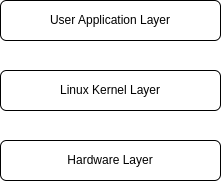
\includegraphics[width=0.3\linewidth]{softarch_mert.png}
    \caption{Software Architecture of the Measurement Network Gateway}
    \label{fig:softarch}
\end{figure}


\subsubsection{Application Layer Design}
The application is responsible for sampling sensor data, storing the sampled data in a 
ring buffer, and transmitting the buffered data to the GUI for graphical visualization. 
In parallel, the application processes commands received from the GUI, enabling 
configuration of sensor sampling frequencies and execution of other gateway-related 
control commands.

The application is composed of three modules: \texttt{mng\_sensor}, \texttt{mng\_network}, and
\texttt{mmng\_ringbuf}. These modules are functionally separated to improve software maintainability and support 
future extensibility.

\begin{figure}[H]
    \centering
    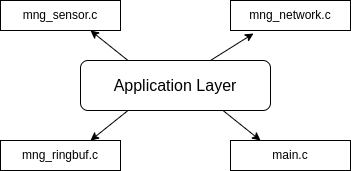
\includegraphics[width=0.5\linewidth]{applayer.png}
    \caption{Modules of Application Layer}
    \label{fig:applayer}
\end{figure}

Each module is accompanied by a corresponding header file. Additionally, a centralized 
configuration header file, \texttt{mng\_config.h}, is used to define macros that are 
shared across the application layer. This design improves code abstraction and 
maintainability by allowing configuration changes to be applied globally without 
requiring modifications to the source code. Such an approach is commonly adopted in 
software architecture design.

Following paragraphs provide a brief overview of the responsibilities of each module. Detailed implementation logic is presented in the implementation section.


\paragraph{MNG\_SENSOR}\

The sensor module is responsible for managing all sensor-related operations. Sensor 
sampling is performed using the Programmable Logic (PL), as in real-world applications 
the number of sensors can exceed 30–50. In such cases, using the PL for high I/O 
requirements is a logical design choice, since typical MCUs do not provide a sufficient 
number of serial communication peripherals, whereas this functionality can be implemented 
in the PL.

Accordingly, the module writes to specific memory-mapped addresses to initiate sensor 
sampling and retrieves the sampled data once the operation is complete. In addition, 
the module updates the timestamp associated with each sensor and accesses sensor 
registers, as each sensor resides in a different address space and is accessed via the 
AXI interface.

Additionally, the module maintains information about each sensor instance, such as 
its ID, register number for access, operational state (active or dormant), sampling 
period, and the sensor frequency selected by the user.

At this stage, only the \texttt{mng\_sensorHandle\_t} structure is presented to illustrate 
the data maintained by the sensor module; detailed source code and implementation 
logic are discussed in the implementation section.


\begin{lstlisting}[caption={MNG Sensor handle structure}, label={lst:sensorhandle}]
typedef struct
{
    uint16_t sensorFreq;     /* Desired Frequency (Hz) set by user. */
    uint16_t samplePeriod;   /* (MNG_BASE_FREQ / sensorFreq)sampling period */
    uint32_t sensorValue;    /* The last sampled data from sensor. */
    uint64_t elapsedTime;    /* Elapsed time between samples. */
    uint8_t  sensorDormant;  /* Sensor active or dormant? */
    uint32_t sensorID;       /* ID of specific sensor */
    uint16_t regNum;         /* Specific register number for sensor object. */
}mng_sensorHandle_t;
\end{lstlisting}


\paragraph{MNG\_RINGBUF}\

Since the application needs to store information about sensors — including their values, 
timestamps, and IDs — a reliable buffer is required before sending the data to the GUI. 
The sensor ID is particularly important, as the GUI identifies sensors based on their 
IDs. A ring buffer is used for this purpose, providing a reliable solution that prevents 
buffer overflow by overwriting the oldest data when the buffer is full.

\begin{lstlisting}[caption={MNG Ring Buffer handle structure}, label={lst:rbufhandle}]
typedef struct mng_rbuf
{
    struct mng_rbuf  * rbufPtr ;                        /* Pointer to self*/
    uint32_t           rbufVal[MNG_RBUF_LENGTH];        /* Sensor Value buffer */
    uint64_t           rbufElpTime[MNG_RBUF_LENGTH];    /* Elapsed time buffer*/
    uint32_t           rbufSensorID[MNG_RBUF_LENGTH];   /* ID for every entry */   
    uint16_t volatile  rbufHead; /* Ptr to where next char will be inserted*/
    uint16_t volatile  rbufTail; /* Ptr to where next char will be extracted*/
    uint16_t           rbufSize; /* Size of the buffer */
    uint16_t volatile  rbufEntries;  /* Current number of entries */
    uint8_t            rbufAlive;    /* Buffer is alive or not info*/
}mng_rbuf_t;
\end{lstlisting}



\paragraph{MNG\_NETWORK}\

The network module establishes a reliable TCP/IP connection with the GUI. It is 
responsible for sending sensor data packets, receiving commands from the client, and 
parsing these commands to perform the corresponding operations in the application.


\begin{lstlisting}[caption={MNG Network handle structure}, label={lst:networkhandle}]
typedef struct
{
    int serverSocket;
    int clientSocket;
    struct sockaddr_in server_address;
    Clnt_Send_struct cmdHandle;
}mng_networkHandle_t;
\end{lstlisting}

Another important data structure in the network module is \texttt{mng\_Payload\_t}, which 
contains the number of samples collected so far, along with the data for each sampled 
sensor, including its value, timestamp, and ID. The payload is transmitted directly to the GUI.

\begin{lstlisting}[caption={MNG Payload structure}, label={lst:payloadhandle}]
typedef struct {
    uint32_t sampleCount;
    mng_sensorDataPacked_t sendBuf[MNG_PAYLOAD_SIZE];
}__attribute__((packed)) mng_Payload_t;
\end{lstlisting}


\subsubsection{Kernel Layer}

This section focuses on the kernel layer of the system, which is implemented using embedded Linux generated with the PetaLinux development framework. PetaLinux simplifies the process of configuring, building, and deploying Linux images for Xilinx platforms through the use of vendor-provided Board Support Packages (BSPs).

A customized Linux image is created and executed on the target Xilinx device, ensuring compatibility between the hardware design and the Linux kernel. This setup enables the development and integration of Loadable Kernel Modules (LKMs), which allow kernel functionality to be extended dynamically.

Since a custom IP core is used to communicate with the sensors, a dedicated kernel module must be developed. In Linux, user-space applications cannot directly access hardware resources; instead, hardware devices are abstracted and exposed through the filesystem. Therefore, the kernel module provides file operations that enable reading from and writing to the device. Additionally, the kernel module must be bound to the appropriate hardware address by defining and associating it with the corresponding device tree entry.

\paragraph{Custom Linux Kernel Module "meascdd"}\

The custom kernel module is first introduced by specifying the device identifier 
to which it is bound. Listing~\ref{lst:meascdd_of_match} shows the device tree 
matching table used to associate the kernel module with the corresponding hardware 
IP core.

\begin{lstlisting}[caption={MNG Payload structure}, label={lst:meascdd_of_match}]
static struct of_device_id meascdd_of_match[] = {
	{ .compatible = "xlnx,measdif-1.0", },
	{ /* end of list */ },
};
\end{lstlisting}

To clarify the meaning of the compatible string "xlnx,measdif-1.0", it is logical 
to present the corresponding device tree entry. This entry defines the custom IP 
core in the hardware description and enables the Linux kernel to match the device 
with the appropriate kernel module. The device tree node shown in 
Listing~\ref{lst:measdif_dts} can be found under the components directory as 
part of the pl.dtsi file, which is automatically generated to describe the 
Programmable Logic design.

\begin{lstlisting}[caption={MNG Payload structure}, label={lst:measdif_dts}]
measdif_0: measdif@43c00000 {
    clock-names = "s00_axi_aclk";
    clocks = <&clkc 15>;
    compatible = "xlnx,measdif-1.0";
    interrupt-names = "md_irq";
    interrupt-parent = <&intc>;
    interrupts = <0 29 4>;
    reg = <0x43c00000 0x10000>;
    xlnx,s00-axi-addr-width = <0x5>;
    xlnx,s00-axi-data-width = <0x20>;
};
\end{lstlisting}


The complete Loadable Kernel Module (LKM) source code is relatively extensive 
and is therefore provided in the appendix. In this section, only the read and 
write operations of the custom kernel module, \texttt{meascdd}, are explained, 
as they are essential for understanding the interaction between the kernel and 
the custom IP core.

Before describing the read and write operations, it is necessary to introduce 
the \texttt{meascdd} header file, as it defines the data structures and macros 
that are directly used during these operations.

\begin{lstlisting}[language=C,
caption={Data structure and macro definitions in the meascdd header file},
label={lst:meascdd_header}]
typedef struct 
{
    unsigned int rnum;
    unsigned int rvalue;
} MeasObj_struct;

#define MEASOBJ_SIZE sizeof(MeasObj_struct)
\end{lstlisting}

The data structure and macro shown in Listing~\ref{lst:meascdd_header} are defined 
in the \texttt{meascdd} header file. This structure is required due to the use 
of a custom IP core. When accessing the IP, the register number must be written 
first in order to specify which register is being addressed, followed by a read 
or write operation to retrieve or update the corresponding register value.

This abstraction allows the kernel module to package register access information 
in a structured manner. The purpose of this design becomes clearer in the 
following text, where the read and write operations of the \texttt{meascdd} 
kernel module are explained in detail.

The write operation of the \texttt{meascdd} kernel module is implemented in the \texttt{dev\_write} function. This function is responsible for handling data sent from user space to the kernel module and forwarding it to the custom IP core when required.

First, the function verifies that the size of the received buffer matches \texttt{MEASOBJ\_SIZE}. This ensures that the incoming data conforms to the expected format defined by the \texttt{MeasObj\_struct} structure. If the buffer size is valid, the data is copied safely from user space to kernel space using \texttt{copy\_from\_user}.

The function then checks the register number field against the \texttt{REGNUM\_ID} macro. If this condition is met, the operation is interpreted as a preparation for a subsequent read operation, and the register number is stored in the global variable \texttt{Reg\_Num}.

If the operation is not a read preparation, the function performs a direct write to the specified register of the custom IP core. The target register address is calculated using the base address of the IP core and the provided register index, and the value is written using \texttt{iowrite32}. In this way, the kernel module supports both register selection and direct register write operations through a unified interface.

\begin{lstlisting}[language=C,
caption={Write operation implementation of the meascdd kernel module},
label={lst:meascdd_write}]
static ssize_t dev_write(struct file *filep,
                         const char *buffer,
                         size_t len,
                         loff_t *offset)
{
    void *reg_addr;

    reg_addr = 0;
    if (len == MEASOBJ_SIZE) 
    {
        copy_from_user(&TF_Obj_Rcv, buffer, len);

        if (TF_Obj_Rcv.rnum == REGNUM_ID) 
        {
            Reg_Num = TF_Obj_Rcv.rvalue;
        } else 
        {
            if (TF_Obj_Rcv.rnum == 0) 
            {
                Led_Output &= 0x080;
                Led_Output |= TF_Obj_Rcv.rvalue & 0x07f;
            }
            reg_addr = (unsigned int)
                       (Meas_Base_Address + 4 * TF_Obj_Rcv.rnum);
            iowrite32(TF_Obj_Rcv.rvalue, reg_addr);
        }
    } else 
    {
        printk(KERN_INFO
               "MEAScdd: [write] len: %d (exp.: %d)\n",
               (int)len, (int)MEASOBJ_SIZE);
    }
    return len;
}
\end{lstlisting}

The read operation of the \texttt{meascdd} kernel module is straightforward. It 
retrieves data from the register that was previously selected during the write 
operation and stored in the global variable \texttt{Reg\_Num}.

When a read request is issued from user space, the \texttt{dev\_read} function 
assigns the selected register number to the outgoing data structure and reads 
the corresponding register value from the custom IP core using \texttt{ioread32}. 
The retrieved register number and value are then copied from kernel space to 
user space using \texttt{copy\_to\_user}.

If the data transfer is successful, the function returns zero, indicating a 
successful read operation. Otherwise, an error code is returned to signal a 
failure in copying data to user space.

\begin{lstlisting}[language=C,
caption={Read operation implementation of the meascdd kernel module},
label={lst:meascdd_read}]
static ssize_t dev_read(struct file *filep,
                        char *buffer,
                        size_t len,
                        loff_t *offset)
{
    int error_count = 0;

    TF_Obj_Snd.rnum = Reg_Num;
    TF_Obj_Snd.rvalue =
        ioread32(Meas_Base_Address + 4 * Reg_Num);

    error_count =
        copy_to_user(buffer, &TF_Obj_Snd, MEASOBJ_SIZE);

    if (error_count == 0) 
    {
        return 0;
    } else 
    {
        printk(KERN_INFO
               "MEAScdd: Failed to send %d characters to the user\n",
               error_count);
        return -EFAULT;
    }
}
\end{lstlisting}




\subsubsection{Hardware Layer}
This section describes the lowest layer of the system, namely the hardware layer. 
The hardware platform used in this project is the ZedBoard development kit, which is
based on the XC7Z020-CLG484 device. This device integrates a dual-core ARM Cortex-A9 
processing system with a Programmable Logic (PL) fabric.

In addition to the processing platform, several external sensors are used, including 
the MAX31865 temperature sensor and the PmodAD1 dual-channel analog-to-digital 
converter (ADC), which provide the necessary sensor data for the system.

\begin{figure}[H]
    \centering
    \includegraphics[width=0.7\linewidth]{zedboard.jpeg}
    \caption{Zedboard}
    \label{fig:zedboard}
\end{figure}


\subsubsection{Data Flow of Program}

Understanding the data flow of the program is crucial for comprehending its overall 
operation. The following figure illustrates how data is transferred from the hardware 
layer to the GUI, as well as how control commands are transmitted from the GUI back to 
the hardware.


\begin{figure}[H]
    \centering
    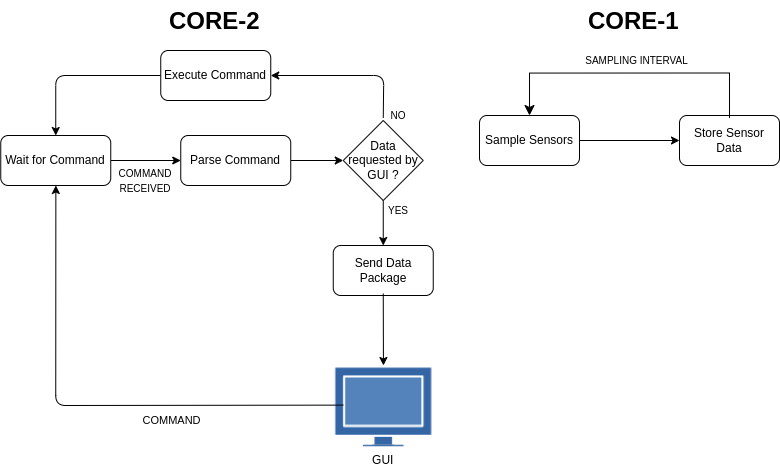
\includegraphics[width=0.9\linewidth]{dataflwww.png}
    \caption{Dataflow of Programme}
    \label{fig:dataflow}
\end{figure}


\subsection{Implementation of Software}
This section presents a detailed explanation of the software implementation. 
Each software module is discussed in depth, with a focus on the key application 
programming interfaces (APIs), internal design decisions, and the overall design 
philosophy of the system.

The software modules are presented in the following order, reflecting their initialization sequence and runtime interaction within the system:

\begin{enumerate}
    \item Main application module
    \item Sensor management module (\texttt{mng\_sensor})
    \item Ring buffer module (\texttt{mng\_ringbuf})
    \item Network communication module (\texttt{mng\_network})
\end{enumerate}


\subsubsection{Main application module}

The main application consists of two separate threads: a sensor thread and a network 
thread. The sensor thread is responsible for sampling sensor data and pushing the 
acquired samples into the ring buffer. The network thread handles the transmission of 
data packets to the GUI, as well as receiving and parsing commands sent by the GUI.
This multi-threaded design enables concurrent data acquisition and network communication, 
improving responsiveness and overall system performance.

In this section, only the core logic of the main application is presented, 
focusing on the sensor and network threads. Initialization routines and auxiliary code 
are omitted for clarity and are provided in the appendix.


\paragraph{Sensor Thread}\

The purpose of the sensor thread is straightforward. At startup, the thread opens the 
device file \texttt{/dev/meascdd} in order to access the custom IP core through the 
kernel module. After successful initialization, the thread enters a continuous execution 
loop.

The execution of this loop is controlled by the runtime variable \texttt{SHUTDOWN}, 
which is exclusively managed by the GUI. This mechanism allows the GUI to remotely 
terminate the application in a controlled manner. Within the loop, sensor data is read 
from the hardware, and upon successful acquisition, the results are written to the ring 
buffer for further processing.

Since the ring buffer is accessed concurrently by both the sensor and network threads, 
a mutex is used to protect shared data and prevent race conditions.

When a shutdown event occurs, the thread exits the loop, closes the \texttt{/dev/meascdd} 
device file, and terminates gracefully.
\newpage
\begin{lstlisting}[language=C,
caption={Sensor Thread Implementation},
label={lst:meascdd_read}]
static void * SensorTask(void *arg)
{
    (void *)arg;
    int fd = open(MNG_MEASCDD_FILE_DESCRIPTOR , O_RDWR);
	if (fd < 0) {
		return errno;
	}
    
    while(SHUTDOWN)
    {
        pthread_mutex_lock(&rbufMutex);
        if (mng_sensorReadADC(&adc0, fd) == MNG_SENSOR_OK)
        {           
            mng_rbufEnqueue(&ringBuff, &adc0);
        }

        if (mng_sensorReadADC(&adc1, fd) == MNG_SENSOR_OK)
        {           
            mng_rbufEnqueue(&ringBuff, &adc1);
        }

        if (mng_sensorReadTemp(&Temperature, fd) == MNG_SENSOR_OK)
        {
            mng_rbufEnqueue(&ringBuff, &Temperature);
        }

        if (mng_sensorRead(&SwitchButtons, fd) == MNG_SENSOR_OK)
        {
            mng_rbufEnqueue(&ringBuff, &SwitchButtons);
        }
        
        pthread_mutex_unlock(&rbufMutex);
        usleep(MNG_SENSOR_LOOP_INTERVAL_US);
    }

    close(fd);
    pthread_exit(NULL);
}
\end{lstlisting}


\paragraph{Network Thread}\

The network thread operates as a TCP server and is responsible for handling communication 
with the GUI client. After initialization, the thread waits for an incoming client 
connection and then blocks on the receive API until a command is sent by the GUI.

The thread executes within a loop controlled by the runtime variable \texttt{SHUTDOWN}. 
Upon receiving a command, the network thread parses the command to determine the requested 
operation. If the command corresponds to a data request, the thread retrieves the number 
of available entries in the ring buffer and dequeues the buffered sensor samples. Since 
the ring buffer is shared with the sensor thread, access is protected using a mutex to 
prevent race conditions.

Each sensor entry consists of a sensor value, a unique sensor ID, and a corresponding 
timestamp. These fields are copied into a payload structure, which is then transmitted 
to the GUI. This design ensures synchronized access to shared data and reliable delivery 
of time-stamped sensor measurements to the client.

\newpage
\begin{lstlisting}[language=C,
caption={Network Thread Implementation},
label={lst:network_thread}]
static void * NetworkThread(void * arg)
{
    (void *)arg;
    int ret;
    mng_networkHandle_t net;
    mng_Payload_t packet;
    int32_t  popVal;
    uint32_t popID;
    uint64_t popTime;

    ret = mng_networkInit(&net);
    if(ret != MNG_NETWORK_OK)
    {
        printf("Error occured in initilization \r\n");
    }

    ret = mng_networkAccept(&net);
    if(ret != MNG_NETWORK_OK)
    {
        printf("Error occured accepting client! \r\n");
    }

    while(SHUTDOWN)
    {
        memset(&net.cmdHandle, 0, sizeof(net.cmdHandle));
        memset(&packet, 0, sizeof(packet));

        ret = mng_networkReceive(&net);
        if(ret == MNG_NETWORK_OK)
        {
            pthread_mutex_lock(&rbufMutex);

            /* Parse the received command */
            mng_networkParseCmd(&net, &ins);

            if(net.cmdHandle.cmd == MNG_CMD_REQ_DATA)
            {
                packet.sampleCount = ringBuff.rbufEntries;

                for(int i = 0;
                    i < packet.sampleCount && i < MNG_PAYLOAD_SIZE;
                    i++)
                {
                    ret = mng_rbufDequeue(&ringBuff,
                                          &popVal,
                                          &popID,
                                          &popTime);
                    if(ret == MNG_RBUF_OK)
                    {
                        packet.sendBuf[i].sensorVal   = popVal;
                        packet.sendBuf[i].sensorID    = popID;
                        packet.sendBuf[i].elapsedTime = popTime;
                    }
                }

                pthread_mutex_unlock(&rbufMutex);

                ret = mng_networkSend(&net,
                                      (mng_Payload_t *)&packet,
                                      sizeof(packet));
                if(ret != MNG_NETWORK_OK)
                {
                    printf("Error occured sending data! \r\n");
                }
            }
            else
            {
                pthread_mutex_unlock(&rbufMutex);
            }
        }
    }

    pthread_exit(NULL);
}
\end{lstlisting}



\subsubsection{Sensor Management Module (\texttt{mng\_sensor})}
The sensor management module (\texttt{mng\_sensor}) is responsible for handling all 
sensor-related operations within the application. It maintains essential information 
for each sensor, including its unique ID, hardware address, operational status, latest 
sampled value, sampling frequency, and timestamp.

Additionally, since the sensors are accessed through a custom IP core, the module manages 
the associated register information and performs the required read and write operations 
to specific registers. This abstraction allows the application to interact with sensors 
in a hardware-independent manner while centralizing sensor control logic within a single 
module.

Since the system supports multiple sensors implemented through custom IP cores, the 
low-level read operations may differ between sensor types. However, the overall design 
philosophy and interaction pattern remain consistent across all sensors.

For this reason, the \texttt{mng\_sensor} module exposes a set of well-defined APIs 
that abstract sensor management and access operations. Some APIs are generic and 
applicable to all sensors, while others are sensor-specific due to hardware differences. 
In this section, the generic APIs are explained in detail, and the sensor-specific 
functions are briefly introduced as they follow a similar operational pattern, but you can find all APIs related to this module in appendix.

\begin{lstlisting}[language=C,
caption={Sensor management module APIs},
label={lst:mng_sensor_api}]
/**
 * @brief Initializes the sensor configuration.
 */
MNG_SENSOR_STAT mng_sensorInit(mng_sensorHandle_t *me,
                               uint16_t userFreq,
                               uint16_t sensorReg,
                               uint32_t id);

/**
 * @brief Samples the sensor.
 */
MNG_SENSOR_STAT mng_sensorRead(mng_sensorHandle_t *me, int fd);

/**
 * @brief Reads a register from the custom IP.
 */
uint32_t mng_readReg(int fd, uint16_t regNum);

/**
 * @brief Writes a value to a register of the custom IP.
 */
void mng_writeReg(int fd, uint16_t regNum, uint32_t regVal);

/**
 * @brief Writes data to the sensor.
 */
MNG_SENSOR_STAT mng_sensorWrite(mng_sensorHandle_t *me,
                                int fd,
                                uint32_t regval);

/**
 * @brief Reads ADC sensor data.
 */
MNG_SENSOR_STAT mng_sensorReadADC(mng_sensorHandle_t *me, int fd);

/**
 * @brief Reads temperature sensor data.
 */
MNG_SENSOR_STAT mng_sensorReadTemp(mng_sensorHandle_t *me, int fd);

/**
 * @brief Calculates system startup time.
 */
uint64_t mng_getStartUpTime(void);

/**
 * @brief Calculates elapsed time between samples.
 */
uint64_t mng_getElapsedTime(void);
\end{lstlisting}

The internal sensor handle structure was introduced in the architecture and design 
section. In this section, the focus shifts to the implementation details of the sensor 
management module, starting with the sensor initialization logic.

\paragraph{mng\_sensorInit\ API}\

The \texttt{mng\_sensorInit} function initializes a sensor handle using user-defined 
configuration parameters. The first parameter is a pointer to the sensor handle structure, 
which represents a specific sensor instance. This handle is later used to manage sampling 
behavior, register access, and runtime state. The remaining parameters specify the 
user-selected sampling frequency, the sensor register number associated with the 
custom IP, and a unique sensor ID.

At the beginning of the function, a null pointer check is performed to ensure that 
the provided sensor handle is valid. This defensive programming approach prevents 
undefined behavior and improves system robustness.

Next, the function verifies that the user-selected frequency is a valid divisor of the 
base frequency, which is defined as 1000~Hz. Since the sensor thread executes at a fixed 
interval of 1~ms, this constraint ensures accurate and deterministic sampling behavior. 
If the frequency is invalid, the function returns an error status and aborts 
initialization.

Once the frequency check succeeds, the sampling period is calculated by dividing the 
base frequency by the selected sensor frequency. This period determines how often the 
sensor will be sampled within the sensor thread loop, which is controlled using a 
conditional check based on the calculated period.

The function then initializes the remaining fields of the sensor handle, including the 
sensor ID, register number, dormant state, elapsed time, and initial sensor value. 
By default, the sensor is configured as active (non-dormant), allowing read and write 
operations to be performed immediately after initialization.

Finally, the function returns a success status, indicating that the sensor has been 
configured correctly and is ready for operation.

\begin{lstlisting}[language=C,
caption={Sensor Initialization API},
label={lst:mng_sensorinit_api}]
MNG_SENSOR_STAT mng_sensorInit (mng_sensorHandle_t * me , uint16_t userFreq 
                                , uint16_t sensorReg , uint32_t id)
{
    if( me == (void *)0 )   /* NULL pointer check*/
    {
        return MNG_SENSOR_ERR_NULL_PTR;
    }

    /* Choosen frequency *MUST* be divided by 10s */
    if((MNG_BASE_FREQ_HZ % userFreq) != 0 )
    {
        me->sensorFreq = 0U;
        return MNG_SENSOR_ERR_FREQ; 
    }

    me->sensorFreq     = userFreq;
    /* Calculate the sample period */
    me->samplePeriod     = MNG_BASE_FREQ_HZ / me->sensorFreq ;
    me->sensorID       = id;
    me->regNum         = sensorReg;
    me->sensorDormant  = 0U;
    me->elapsedTime    = 0U;
    me->sensorValue    = 0U;

    return MNG_SENSOR_OK;
}
\end{lstlisting}


\paragraph{mng\_sensorRead API}\

The sensor read logic implemented in \texttt{mng\_sensorRead} follows a deterministic 
and time-driven approach. The function is invoked periodically by the sensor thread, 
which executes at a fixed interval of 1~ms.

At the beginning of the function, the sensor’s operational state is checked. If the 
sensor is marked as dormant, the function immediately returns without performing any 
read operation. This mechanism allows sensors to be dynamically enabled or disabled 
during runtime.

If the sensor is active, the function decrements the internal \texttt{samplePeriod} 
counter. When this counter reaches zero, it indicates that the configured sampling 
interval has elapsed and the sensor should be sampled. In this case, the sensor value 
is read from the corresponding register using the register access abstraction. After 
sampling, the \texttt{samplePeriod} counter is reinitialized to its original value to 
schedule the next read operation.

Additionally, the elapsed time since system startup is recorded at the moment of 
sampling. This timestamp is later used to associate each sensor measurement with a 
precise time reference. If the sampling condition is not met, the function returns a 
wait status, indicating that the sensor is not yet ready to be sampled.

The sampling period is calculated during sensor initialization by dividing the base frequency by the user-selected sampling frequency. The base frequency is defined as 1000~Hz, which corresponds to the execution rate of the sensor thread (1~ms per iteration). This calculation determines how many thread iterations must occur before a sensor is sampled.

\begin{quote}
Assume that the user selects a sampling frequency of 100~Hz.  
Since the sensor thread executes every 1~ms, the sensor must be sampled every 10~ms.

\[
\text{samplePeriod} = \frac{\text{MNG\_BASE\_FREQ\_HZ}}{\text{userFreq}} =
\frac{1000}{100} = 10
\]

This means that the sensor read operation is performed once every 10 iterations of the sensor thread loop.
\end{quote}


\begin{lstlisting}[language=C,
caption={Sensor Read API},
label={lst:mng_sensorRead_api}]
MNG_SENSOR_STAT mng_sensorRead(mng_sensorHandle_t * me , int fd)
{
    /* Check if sensor is in Wait mode. */
    if(me->sensorDormant != 0U)
    {
        return MNG_SENSOR_DORMANT;
    }

    me->samplePeriod--;
    /*  Read sensor if counter is finished. */
    if(me->samplePeriod == 0U)
    {
        me->sensorValue = mng_readReg( fd , me->regNum );
        /* Set counter for future reading. */
        me->samplePeriod = MNG_BASE_FREQ_HZ / me->sensorFreq;
        /* Get elapsed time */
        me->elapsedTime = mng_getElapsedTime();

        return MNG_SENSOR_OK;
    }

    return MNG_SENSOR_WAIT;
}
\end{lstlisting}


\paragraph{mng\_sensorWrite API}\

The \texttt{mng\_sensorWrite} function provides a generic interface for writing 
configuration or control values to a sensor through the custom kernel module. Similar 
to the read operation, the function first checks whether the sensor is in a dormant state. 
If the sensor is inactive, write operations are prevented and the function returns 
immediately.

For write operations, the same data structure used by the kernel driver is employed. 
A local instance of the measurement object structure is populated with the target 
register number and the value to be written. This structure is then passed to the kernel 
module using the standard \texttt{write()} system call.

By reusing the kernel module’s data format, the application maintains a consistent and 
simple communication mechanism between user space and kernel space. If the write operation 
fails, an error status is returned; otherwise, the function reports successful completion.


\begin{lstlisting}[language=C,
caption={Sensor Write API},
label={lst:mng_sensorWrite_api}]
MNG_SENSOR_STAT mng_sensorWrite (mng_sensorHandle_t * me , int fd , uint32_t regval)
{
    int ret;
    /* Check if sensor is in Wait mode. */
    if(me->sensorDormant != 0U)
    {
        me->sensorValue = 0U;
        return MNG_SENSOR_DORMANT;
    }

    MeasObj_struct TF_Obj_Snd;
    TF_Obj_Snd.rnum   = me->regNum;
    TF_Obj_Snd.rvalue = regval;

    ret = write(fd , &TF_Obj_Snd , MEASOBJ_SIZE);
    if(ret < 0)
    {
        return MNG_SENSOR_ERR_FREQ;
    }

    return MNG_SENSOR_OK;
}
\end{lstlisting}


\paragraph{mng\_getStartUpTime API}\

At the beginning of the program, the startup time is recorded to serve as a reference 
for elapsed time calculations during runtime. The \texttt{mng\_getStartUpTime} function 
retrieves this initial timestamp and stores it in microsecond resolution.

The function calls the \texttt{clock\_gettime()} system API with the 
\texttt{CLOCK\_MONOTONIC} clock source. This clock is managed by the Linux kernel and is 
typically backed by hardware timers within the CPU or system-on-chip. The monotonic clock 
guarantees that the reported time always increases monotonically and is not affected by 
system time adjustments, making it suitable for precise time measurements.

The returned time consists of seconds and nanoseconds, which are converted into microseconds before being returned. This conversion provides sufficient temporal resolution for sensor timestamping while keeping the arithmetic simple and efficient.

\begin{lstlisting}[language=C,
caption={Start Up Time API},
label={lst:mng_getStartup_api}]
uint64_t mng_getStartUpTime(void)
{
    struct timespec startupTime;
    startupTime.tv_nsec = 0U;
    startupTime.tv_sec = 0U;
    /* Get startup time */
    clock_gettime(CLOCK_MONOTONIC, &startupTime);
    /* Calculation to get time in microsecond */
    return ((startupTime.tv_sec * 1000000U) + (startupTime.tv_nsec / 1000U));
}
\end{lstlisting}

\paragraph{mng\_getElapsedTime API}\

The \texttt{mng\_getElapsedTime} function calculates the elapsed time since the 
application startup and returns this value in microseconds. This function follows a 
structure similar to the startup time API and relies on the same monotonic clock source 
to ensure consistency and reliability.

During execution, the function retrieves the current time using the \texttt{clock\_gettime()}
API with the \texttt{CLOCK\_MONOTONIC} clock. The returned timestamp, represented in 
seconds and nanoseconds, is converted into microseconds for uniformity with the startup 
time representation.

The elapsed time is then calculated by subtracting the globally stored startup time value from the current timestamp. This approach provides a simple and efficient mechanism for generating precise timestamps for sensor samples, enabling each measurement to be associated with an accurate time reference relative to system startup.


\begin{lstlisting}[language=C,
caption={Elapsed Time API},
label={lst:mng_getElapsedTime_api}]
uint64_t mng_getElapsedTime (void)
{
    static struct timespec currentTime;
    uint64_t usCurrentTime;
    uint64_t elapsedTime;

    /* Get current time */
    clock_gettime(CLOCK_MONOTONIC, &currentTime);

    /* Calculation to get time in microsecond */
    usCurrentTime =((currentTime.tv_sec*1000000U)+(currentTime.tv_nsec / 1000U));
    elapsedTime   = usCurrentTime - usStartupTime;

    return elapsedTime; /* return elapsed time */
}
\end{lstlisting}


\subsubsection{Ring Buffer Module (\texttt{mng\_ringbuf})}

Sensor measurements must be temporarily stored before being transmitted to the GUI through 
the network module. To support this requirement, the application employs a ring buffer 
data structure to store sampled sensor entries in a reliable and memory-efficient manner.

A ring buffer is particularly well suited for this type of application, as it prevents 
buffer overflow by overwriting the oldest data when the buffer becomes full. This 
behavior ensures continuous operation even under high sampling rates or temporary 
communication delays. Each buffer entry contains the sensor value, sensor ID, and 
corresponding timestamp, allowing the network module to transmit complete and time-stamped 
sensor data to the client.

The \texttt{mng\_ringbuf} module provides a small set of APIs to manage buffer creation 
and data flow, including buffer initialization, enqueue, and dequeue operations. These 
APIs are explained in detail in the following paragraphs.

\paragraph{Ring Buffer Creation API (\texttt{mng\_rbufCreate})}\

The \texttt{mng\_rbufCreate} function is responsible for initializing a ring buffer 
instance before it is used by the application. During initialization, internal control 
variables such as the number of stored entries, head index, and tail index are reset to 
zero. This ensures that the buffer starts in a known and consistent state.

The function also sets an internal status flag indicating that the buffer is active. 
This flag is used to validate buffer operations during runtime and prevents enqueue or 
dequeue operations on an uninitialized buffer.

An important design decision in this module is that the ring buffer length is fixed at 
compile time using the \texttt{MNG\_RBUF\_LENGTH} macro. This choice is motivated by 
performance and networking constraints. Since sensor data is transmitted over TCP/IP, 
the payload size is intentionally limited to ensure that each data packet fits within a 
single Ethernet frame and does not exceed the maximum transmission unit (MTU) of 
approximately 1500 bytes. In the current implementation, the buffer length is set to 
104 entries, guaranteeing that a complete payload can be sent without fragmentation.

Finally, the function clears all buffer storage arrays, including sensor values, sensor 
IDs, and elapsed time fields. Initializing these memory regions to zero prevents 
residual or invalid data from being transmitted during early operation. Upon successful 
completion, the function returns a success status, indicating that the ring buffer is 
ready for use.

\begin{lstlisting}[language=C,
caption={Ring Buffer Create API},
label={lst:mng_rbufCreate_api}]
MNG_RBUF_STAT mng_rbufCreate(mng_rbuf_t * me )
{
    if (me == (void *)0 ) /* Check if pointer is NULL */
    {
        return MNG_RBUF_ERR_NULL_PTR;
    }

    me->rbufPtr      = me;           /* Pointer to object*/
    me->rbufEntries  = 0U;
    me->rbufHead     = 0U;
    me->rbufTail     = 0U;
    me->rbufAlive    = 1U;
    me->rbufSize     = MNG_RBUF_LENGTH;

    /* Clear Content of adresses, elapsed time and id space. */
    for(uint16_t i=0 ; i < me->rbufSize ; i++ )
    {
        me->rbufVal[i]      = 0U;
        me->rbufSensorID[i] = 0U;
        me->rbufElpTime[i]  = 0U;
    }

    return MNG_RBUF_OK;
}
\end{lstlisting}

\paragraph{Ring Buffer Enqueue API (\texttt{mng\_rbufEnqueue})}\

The \texttt{mng\_rbufEnqueue} function inserts a new sensor sample into the ring buffer. 
This function is typically called by the sensor thread after a successful sensor read 
operation and acts as the producer interface of the buffer.

At the beginning of the function, defensive checks are performed to ensure that the 
buffer pointer is valid and that the buffer instance is active. If the buffer has not 
been properly initialized or has been marked inactive, the function returns an error 
status to prevent undefined behavior.

Before inserting new data, the function checks whether the buffer is full. If the buffer 
has reached its maximum capacity, two behaviors are possible depending on the compilation 
configuration. When the overwrite mode is enabled, the oldest buffer entry is discarded 
by advancing the tail index, thereby making room for the new data. This approach 
ensures continuous operation without blocking the producer. If overwrite mode is 
disabled, the function reports a buffer-full error and rejects the new entry.

Once space is available, the sensor’s value, unique sensor ID, and elapsed timestamp 
are written to the current head position of the buffer. After storing the data, the 
head index is advanced using modular arithmetic to maintain the circular structure of 
the ring buffer. Finally, the number of stored entries is incremented, and the function 
returns a success status.

\begin{lstlisting}[language=C,
caption={Ring Buffer Enqueue API},
label={lst:mng_rbufEnqueue_api}]
MNG_RBUF_STAT mng_rbufEnqueue (mng_rbuf_t * me , mng_sensorHandle_t * sensor)
{
    if (me == (void *)0 ) /* Check if pointer is NULL */
    {
        return MNG_RBUF_ERR_NULL_PTR;
    }

    if(me->rbufAlive == 0U) /* is Alive? */
    {
        return MNG_RBUF_ERR_DEAD;
    }

    if (me->rbufEntries == me->rbufSize)
    {
#ifdef MNG_RBUF_OVERWRITE
    /* Overwrite: remove oldest item */
    me->rbufTail = (me->rbufTail + 1U) % me->rbufSize;
    me->rbufEntries--;
#else
    return MNG_RBUF_ERR_FULL;
#endif
    }

    /* Write sensor value to buffer. */
    me->rbufVal[me->rbufHead] = sensor->sensorValue; 
    /* Give ID number for specific sensor value. */
    me->rbufSensorID[me->rbufHead] = sensor->sensorID;
    /* Write elapsed time to buffer */
    me->rbufElpTime[me->rbufHead] = sensor->elapsedTime;           
    
    me->rbufHead =  ( me->rbufHead + 1U ) % me->rbufSize; /* Determine next inserted buf area*/
    me->rbufEntries++;                                    /* Increase entries by one */
    return MNG_RBUF_OK;
}
\end{lstlisting}

\paragraph{Ring Buffer Dequeue API (\texttt{mng\_rbufDequeue})}\

The \texttt{mng\_rbufDequeue} function removes and returns the oldest sensor entry 
stored in the ring buffer. This function represents the consumer interface of the 
buffer and is typically used by the network thread when preparing sensor data packets 
for transmission to the GUI.

The first parameter is a pointer to the ring buffer instance. The remaining parameters 
are output pointers used to return the dequeued sensor value, sensor ID, and elapsed 
timestamp to the caller. By using output parameters, the function avoids unnecessary 
data copying and allows the caller to directly retrieve individual fields of a sensor 
entry.

At the beginning of the function, validity checks are performed to ensure that the 
buffer pointer is not null and that the buffer instance is active. If the buffer has 
not been initialized or has been marked inactive, an error status is returned.

The function then checks whether the buffer contains any entries. If the buffer is 
empty, a specific empty-buffer error is returned to indicate that no data is available 
for extraction.

When valid data is present, the function retrieves the sensor value, sensor ID, and 
elapsed time from the current tail position of the buffer and stores them in the 
corresponding output parameters. After the data is extracted, the tail index is advanced 
using modular arithmetic to preserve the circular structure of the ring buffer, and 
the entry count is decremented. Finally, the function returns a success status.

\begin{lstlisting}[language=C,
caption={Ring Buffer Dequeue API},
label={lst:mng_rbufDequeue_api}]
MNG_RBUF_STAT mng_rbufDequeue (mng_rbuf_t * me , uint32_t * sensor_val ,
                                 uint32_t * id , uint64_t * elapsedTime)
{
    if (me == (void *)0 ) /* Check if pointer is NULL */
    {
        return MNG_RBUF_ERR_NULL_PTR;
    }

    if(me->rbufAlive == 0U)/* is Alive? */
    {
        return MNG_RBUF_ERR_DEAD; // add error macros here
    }

    /* Check if there is any entry to buffer ? */
    if(me->rbufEntries == 0U)
    {
        return MNG_RBUF_ERR_EMPTY;
    }
    
    /* De-reference sensor value from buffer. */
    *sensor_val = me->rbufVal[me->rbufTail];
    /* De-reference sensor ID from buffer. */
    *id = me->rbufSensorID[me->rbufTail];
    /* De-reference elapsed time from buffer. */
    *elapsedTime = me->rbufElpTime[me->rbufTail];
    /* Determine next extracted buf area*/
    me->rbufTail=  ( me->rbufTail + 1U ) % me->rbufSize; 
    me->rbufEntries--;             /* Decrease entries by one */
    
    return MNG_RBUF_OK;
}
\end{lstlisting}


\subsubsection{Network Communication Module (\texttt{mng\_network})}

The network module (\texttt{mng\_network}) is responsible for establishing and managing 
communication between the embedded system and the graphical user interface (GUI). 
It provides a reliable TCP/IP-based interface for transmitting sensor data and 
receiving control commands from the client.

Within the application architecture, the network module operates as a TCP server. It 
listens for incoming connections from the GUI, accepts client requests, and processes 
commands in a blocking manner. Based on the received commands, the module either 
transmits buffered sensor data or modifies the runtime behavior of the system, such as 
sampling configuration or shutdown control.

To maintain modularity and separation of concerns, all socket creation, connection 
handling, data transmission, and command parsing logic are encapsulated within this 
module. This abstraction allows the main application and other modules to interact with 
the network layer through a small and well-defined set of APIs, without direct 
dependency on low-level networking details.

In the following subsections, the core APIs provided by the \texttt{mng\_network} module 
are described, focusing on connection establishment, data exchange, and command 
handling mechanisms.


\paragraph{Network Initialization API (\texttt{mng\_networkInit})}\

The \texttt{mng\_networkInit} function initializes the network module and prepares the 
application to operate as a TCP server. The function begins by validating the provided 
network handle pointer to ensure that it is not null.

During initialization, both the server and client socket descriptors are set to an 
invalid state, indicating that no active connections exist. The function then creates 
a TCP socket using the IPv4 address family and stream-based communication. If socket 
creation fails, an appropriate error status is returned.

After successfully creating the socket, the server address structure is configured. 
The server is bound to all available network interfaces using \texttt{INADDR\_ANY}, and 
a predefined port number is assigned. This configuration allows the GUI client to connect 
to the embedded system regardless of the specific network interface used.

The socket is then bound to the configured address and placed into a listening state. 
By calling the listen operation, the server becomes ready to accept incoming connection 
requests from the GUI. Any failure during the binding or listening stages results in an 
error return value.

Upon successful completion, the function returns a success status, indicating that the 
network module is initialized and ready to accept client connections.


\begin{lstlisting}[language=C,
caption={Network Initialization API},
label={lst:mng_networkInit_api}]
MNG_NETWORK_STAT mng_networkInit (mng_networkHandle_t * me )
{
    int ret;

    if(me == (void *)0)
    {
        return  MNG_NETWORK_ERR_NULL_PTR;
    }

    /* Initialize server and client to disconnected */
    me->serverSocket = -1 ;
    me->clientSocket = -1 ;

    /* Create socket file descriptor. */
    me->serverSocket = socket(AF_INET , SOCK_STREAM , 0);
    if(me->serverSocket < 0)
    {
        return MNG_NETWORK_ERR_SOCKET;
    }
    
    /* Configuring server address structure. */
    me->server_address.sin_family = AF_INET;
    me->server_address.sin_addr.s_addr = INADDR_ANY;
    me->server_address.sin_port = htons(MNG_NETWORK_PORT);

    /* Bind the socket. */
    ret = bind(me->serverSocket , (struct sockaddr *)&me->server_address , 
                                                    sizeof(me->server_address));
    if(ret < 0 )
    {
        return MNG_NETWORK_ERR_BIND;
    }

    /* Listen for connection from GUI (client) */
    ret = listen(me->serverSocket , 2);
    if(ret < 0 )
    {
        return MNG_NETWORK_ERR_LISTEN;
    }

    return     MNG_NETWORK_OK;
}
\end{lstlisting}

\newpage
\paragraph{Network Accept API (\texttt{mng\_networkAccept})}\

The \texttt{mng\_networkAccept} function is responsible for accepting an incoming 
connection request from the GUI client. This function is called after the network 
module has been successfully initialized and the server socket has been placed into a 
listening state.

At the beginning of the function, a null pointer check is performed to ensure the 
validity of the network handle. The function then invokes the \texttt{accept()} system 
call on the server socket. This call is blocking, meaning that the function execution 
is suspended until a client establishes a connection. This behavior is intentional 
and ensures that the application does not proceed with data exchange before a valid 
client connection is available.

Upon a successful connection, a new socket descriptor is created for the client and 
stored in the network handle. This client socket is subsequently used for all data 
transmission and reception operations between the embedded system and the GUI. If the 
accept operation fails, the function returns an error status.

Once a client connection has been accepted, the function returns a success status, 
indicating that the system is ready for bidirectional communication.

\begin{lstlisting}[language=C,
caption={Network Accept API},
label={lst:mng_networkAccept_api}]
MNG_NETWORK_STAT mng_networkAccept (mng_networkHandle_t * me )
{
    if(me == (void *)0)
    {
        return MNG_NETWORK_ERR_NULL_PTR;
    }

    /* Accepting the client */
    /*******                !IT BLOCKS HERE!     **********/
    me->clientSocket = accept(me->serverSocket , NULL ,NULL);
    if( me->clientSocket < 0 )
    {
        return MNG_NETWORK_ERR_ACCEPT;
    }
    
    return MNG_NETWORK_OK;
}
\end{lstlisting}


\paragraph{Network Receive API (\texttt{mng\_networkReceive})}\

The \texttt{mng\_networkReceive} function is responsible for receiving commands sent by 
the GUI client. This function operates on the client socket established during the 
connection acceptance phase and is typically called within the network thread’s main 
loop.

The function begins by validating the network handle pointer. It then invokes the 
\texttt{recv()} system call to read incoming data from the client socket into the 
command handling structure. This call is blocking and waits until data is available, 
the connection is closed, or an error occurs.

If the receive operation returns a negative value, an error status is reported, 
indicating a communication failure. If the return value is zero, it signifies that the 
remote client has closed the connection. In this case, the client socket is closed, and 
a specific status code is returned to notify the application of the disconnection.

When valid data is successfully received, the function returns a success status. The 
received command is stored in the internal command handle structure and is later 
processed by the command parsing API to determine the appropriate action.

\newpage
\begin{lstlisting}[language=C,
caption={Network Receive API},
label={lst:mng_networkReceive_api}]
MNG_NETWORK_STAT mng_networkReceive (mng_networkHandle_t * me )
{
    ssize_t len;
    if(me == (void *)0)
    {
        return MNG_NETWORK_ERR_NULL_PTR;
    }

    len = recv(me->clientSocket , &me->cmdHandle , sizeof(Clnt_Send_struct) , 0);
    if(len < 0 )
    {
        return MNG_NETWORK_ERR_RECV;

    }
    else if(len == 0)  /* Connection closed by remote client*/
    {
        mng_networkCloseClient(me); 
        return MNG_NETWORK_CLIENT_CLOSED;
    }
    else if(len > 0)
    {
        return MNG_NETWORK_OK;
    }
}
\end{lstlisting}


\paragraph{Network Send  API (\texttt{mng\_networkSend})}\

The \texttt{mng\_networkSend} function is responsible for transmitting data from the 
embedded system to the GUI client over the established TCP connection. This function is 
primarily used to send sensor data payloads prepared by the network thread after 
processing client requests.

The function begins by validating the network handle pointer to ensure that the network 
module has been properly initialized. It then uses the \texttt{send()} system call to 
transmit the provided data buffer over the client socket. The length parameter specifies 
the exact number of bytes to be sent, allowing structured data such as sensor payloads 
to be transmitted in a single operation.

If the send operation fails, an appropriate error status is returned to notify the 
application of the transmission failure. Otherwise, the function returns a success 
status, indicating that the data has been successfully delivered to the client.

\begin{lstlisting}[language=C,
caption={Network Send API},
label={lst:mng_networkSend_api}]
MNG_NETWORK_STAT mng_networkSend (mng_networkHandle_t * me , const void * data , size_t len)
{
    int ret;
    if(me == (void *)0)
    {
        return MNG_NETWORK_ERR_NULL_PTR;
    }

    ret = send(me->clientSocket , data , len , 0);
    if(ret < 0 )
    {
        return MNG_NETWORK_ERR_SEND;
    }

    return MNG_NETWORK_OK;
}
\end{lstlisting}


\paragraph{Network Parse Command API (\texttt{mng\_networkParseCmd})}\

Commands sent by the GUI client are encapsulated in a structured data format defined by 
the \texttt{Clnt\_Send\_struct} type. This structure is used both on the embedded system 
and the GUI side to ensure that the command format is identical and consistent across 
both platforms.

The structure contains two primary components:

\begin{enumerate}
    \item \textbf{cmd:} An unsigned integer that specifies the type of command being sent. This field informs the embedded system which action to perform, such as requesting sensor data, changing sensor frequency, or initiating shutdown.
    
    \item \textbf{param:} An array of unsigned integers of size \texttt{MNG\_CMD\_MAX\_PARAMS}. Each element provides additional information related to the command. 
    \begin{itemize}
        \item For example, in a sensor frequency change command, \texttt{param[0]} may indicate the sensor ID to update, and \texttt{param[1]} specifies the new sampling frequency. 
        \item Additional indices can be used for other command-specific parameters.
    \end{itemize}
\end{enumerate}

The structure is declared with the \texttt{\_\_attribute\_\_((packed))} attribute to 
prevent compiler-inserted padding. This ensures that the memory layout is deterministic 
and compatible across the embedded system and GUI, which is critical for reliable network 
transmission.

\begin{lstlisting}[language=C,
caption={Send Command Structure},
label={lst:Clnt_Send_struct}]
typedef struct {
    unsigned int cmd;                   
    unsigned int param[MNG_CMD_MAX_PARAMS];     
} __attribute__((packed)) Clnt_Send_struct;
\end{lstlisting}


The \texttt{mng\_networkParseCmd} function is responsible for interpreting and acting on commands received from the GUI. This API is invoked immediately after a command is received by the network task, ensuring that every incoming message is parsed and handled consistently before further processing.

The command parser is designed to be easily extensible; new commands can be added by introducing new command identifiers and corresponding case blocks. In the current implementation, the system supports several different command types, each serving a specific purpose in controlling the application and the sensors.

One possible command is a data request command. In this case, the parser does not perform any action and simply returns. The actual data handling logic is implemented in the network task itself, which prepares the payload and sends it back to the GUI.

Several commands are used to control sensor activity by placing individual sensors into dormant mode. Depending on the received command, the corresponding sensor instance (ADC0, ADC1, temperature sensor, or switch/button sensor) is marked as dormant. When a sensor is in dormant mode, it is excluded from sampling and write operations, effectively disabling it without removing it from the system.

The parser also supports write operations to the hardware, such as writing values to the LED register. In this case, the parser opens the custom kernel module device file and writes the requested value to the appropriate register using the low-level register access API. This allows the GUI to directly control hardware outputs.

Another important command handled by the parser is the shutdown command. When this command is received, a global runtime variable is updated, which causes all application threads to exit their main loops gracefully. This mechanism allows the GUI to remotely terminate the application in a controlled manner.

Finally, the parser supports dynamic sensor frequency configuration. When a frequency update command is received, the parser identifies the target sensor using the first parameter and updates the sensor’s sampling frequency using the second parameter. At the same time, the sensor is taken out of dormant mode to ensure that sampling resumes immediately with the new configuration.

Overall, \texttt{mng\_networkParseCmd} function acts as a central decision point between the GUI and the application logic, translating high-level GUI commands into concrete actions such as sensor control, frequency configuration, hardware register access, and application shutdown.


\begin{lstlisting}[language=C,
caption={Network Parser API},
label={lst:payloads}]
void mng_networkParseCmd (mng_networkHandle_t * me , mng_sensorInstances_t * s)
{
    switch (me->cmdHandle.cmd)
    {
        case MNG_CMD_REQ_DATA:            
            break;

        case MNG_CMD_DORMANT_ADC0:
            /* code */
            s->adc0Instance->sensorDormant = 1U;
            break;
        
        case MNG_CMD_DORMANT_ADC1:
            /* code */
            s->adc1Instance->sensorDormant = 1U;
            break;

        case MNG_CMD_DORMANT_TEM:
            /* code */
            s->tempInstance->sensorDormant = 1U;
            break;

        case MNG_CMD_DORMANT_SWBUTT:
            /* code */
            s->SwitchButtonsInstance->sensorDormant = 1U;
            break;

        case MNG_CMD_WLED:
            /* code */
            // Write to leds
            int fd = open(MNG_MEASCDD_FILE_DESCRIPTOR , O_RDWR);
            mng_writeReg(fd , MNG_IP_LEDS_REGNUM , me->cmdHandle.param[0]);
            break;

        case MNG_CMD_SHUTDOWN:
            /* code */
            SHUTDOWN = 0;
            break;

        case MNG_CMD_SET_FREQ:
            /* code */
            if ( me->cmdHandle.param[0] == MNG_CMD_SET_FREQ_ADC0)
            {
                s->adc0Instance->sensorDormant = 0U;   
                s->adc0Instance->sensorFreq = me->cmdHandle.param[1];
            }
            else if(me->cmdHandle.param[0] == MNG_CMD_SET_FREQ_ADC1)
            {
                s->adc1Instance->sensorDormant = 0U;
                s->adc1Instance->sensorFreq = me->cmdHandle.param[1];
                printf(" TEMP FREQ HAS CHANGED\n");
            }
            else if(me->cmdHandle.param[0] == MNG_CMD_SET_FREQ_TMP)
            {
                s->tempInstance->sensorDormant = 0U;
                s->tempInstance->sensorFreq = me->cmdHandle.param[1];
            }
            else if(me->cmdHandle.param[0] == MNG_CMD_SET_FREQ_SWBT)
            {
                s->SwitchButtonsInstance->sensorDormant = 0U;
                s->SwitchButtonsInstance->sensorFreq = me->cmdHandle.param[1];
            }

            break;

        default:
            break;
    }
} 
\end{lstlisting}


\paragraph{Network Payload Structure}\

Lastly, this section presents the data payload that is transmitted from the embedded 
system to the GUI application. The payload structure, named \texttt{mng\_Payload\_t}, 
is designed to efficiently encapsulate sampled sensor data and transmit it over the 
TCP/IP connection.

The payload consists of two main components. The first field, \texttt{sampleCount}, 
indicates the number of valid sensor samples contained in the current payload. This 
allows the GUI to correctly interpret how many sensor entries are included in a single 
transmission.

The second component is an array of \texttt{mng\_sensorDataPacked\_t} structures. Each 
entry in this array represents one sensor sample and contains the elapsed time since 
system startup, the sampled sensor value, and a sensor-specific identifier. This design 
allows the GUI to distinguish between different sensors and associate each measurement 
with an accurate timestamp.

Both structures are declared with the \texttt{\_\_attribute\_\_((packed))} attribute. 
This ensures that no compiler-introduced padding bytes are added, resulting in a 
deterministic and compact memory layout. Such a layout is critical for network 
transmission, as it guarantees consistency between the embedded system and the GUI 
regardless of platform or compiler differences.

The payload size is bounded by the \texttt{MNG\_PAYLOAD\_SIZE} macro, which is chosen 
to ensure that the complete payload fits within a single TCP/IP packet. This minimizes 
fragmentation and improves transmission efficiency and reliability.

\begin{lstlisting}[language=C,
caption={Network Payload Structures},
label={lst:payloads}]
typedef struct {
    uint64_t  elapsedTime;   /* Time Info */
    uint32_t  sensorVal;     /* Sensor sampled data*/
    uint32_t  sensorID;      /* Sensor specific ID*/
}__attribute__((packed)) mng_sensorDataPacked_t;


typedef struct {
    uint32_t sampleCount;
    mng_sensorDataPacked_t sendBuf[MNG_PAYLOAD_SIZE];
}__attribute__((packed)) mng_Payload_t;
\end{lstlisting}

\subsubsection{Software Configuration (\texttt{mng\_config})}

The \texttt{mng\_config} file is the central configuration header for the application layer.
 It defines all compile-time parameters that control the behavior of the software, 
 including buffer sizes, timing parameters, network settings, sensor identifiers, 
 and command definitions. By collecting these parameters in a single configuration 
 file, the application becomes easier to maintain, extend, and adapt to new 
 requirements without modifying the core implementation.

One of the most important configuration groups is related to buffer management. 
The ring buffer length is defined by \texttt{MNG\_RBUF\_LENGTH}, which determines how many 
sensor samples can be stored before transmission to the GUI. The optional 
\texttt{MNG\_RBUF\_OVERWRITE} macro enables overwrite behavior, allowing the buffer to replace 
the oldest data when it becomes full. This approach prevents buffer overflow and 
ensures continuous operation in long-running systems.

The configuration file also defines timing and sampling parameters. The macro 
\texttt{MNG\_BASE\_FREQ\_HZ} specifies the base frequency of the sensor sampling loop, which 
is fixed at 1000 Hz. This value represents the maximum sampling resolution of the 
system. The sensor thread sleeps for \texttt{MNG\_SENSOR\_LOOP\_INTERVAL\_US} 
microseconds, resulting in a 1 ms loop period. Initial sensor sampling frequency 
is set using \texttt{MNG\_INITIAL\_FREQ\_HZ}, allowing sensors to start with a known and safe 
default rate.

Network-related parameters are also configured in this file. The TCP/IP server 
port is defined by \texttt{MNG\_NETWORK\_PORT}, and the maximum number of command parameters 
is controlled by \texttt{MNG\_CMD\_MAX\_PARAMS}. These macros ensure consistent communication 
behavior between the embedded system and the GUI.

The file further includes hardware-related definitions, such as the device file 
path of the custom kernel module (/dev/meascdd) and register numbers for different 
sensors and peripherals. Since the application communicates with a custom IP core, 
register numbers such as ADC, temperature sensor, switch/button inputs, and LED 
outputs must be defined explicitly. Placing these definitions in the configuration 
file allows hardware changes to be handled with minimal software modification.

Each sensor is also assigned a unique sensor ID, which is used throughout the 
application and by the GUI to identify sensor data. These IDs ensure that sensor 
samples remain distinguishable when transmitted over the network.

Another critical configuration group is the payload and command definitions. 
The \texttt{MNG\_PAYLOAD\_SIZE} macro determines how many sensor samples are included in a 
single network packet. This value is carefully selected to ensure that the total 
packet size remains below the Ethernet MTU limit, preventing IP fragmentation. 
Command macros define all supported client–server interactions, such as requesting 
data, setting sensors to dormant mode, changing sampling frequency, writing to LEDs,
and shutting down the application.

Finally, the configuration file declares the global SHUTDOWN variable, which is 
used as a runtime control flag shared across threads. This variable allows the GUI 
to safely terminate the application by signaling all threads to exit their execution 
loops.

Overall, \texttt{mng\_config} provides a clean separation between configuration and 
implementation. This design improves code readability, enhances portability, and 
allows rapid system tuning without requiring invasive code changes.



\begin{lstlisting}[language=C,
caption={Software Configuration Header File},
label={lst:config}]
#ifndef MNG_CONFIG_H
#define MNG_CONFIG_H


/* Length of the Ring Buffer*/
#define MNG_RBUF_LENGTH                  104U
/* Overwrite of sampled datas to buffer *Uncomment to use*  */
#define MNG_RBUF_OVERWRITE
/* Base frequency is maximum frequency that sensor can sampled. */
#define MNG_BASE_FREQ_HZ                 1000U
/* 1 ms sensor loop sleep value. (microsec) */     
#define MNG_SENSOR_LOOP_INTERVAL_US      1000
/* Initial frequency  for sampling sensors is 10 Hz */
#define MNG_INITIAL_FREQ_HZ              10U
/* Command buffer to store client's commands. */
#define MNG_CMD_MAX_PARAMS               2
/* Network port for server. */
#define MNG_NETWORK_PORT                 50012
/* Network Timeout Value in us for Select API */
#define MNG_NETWORK_TIMEOUT_US           1000
/* Meascdd device driver file descriptor directory. */
#define MNG_MEASCDD_FILE_DESCRIPTOR      "/dev/meascdd"
/* ADC Sensor Register Number*/
#define MNG_IP_ADC_SENSOR_REGNUM         5
/* MAX Sensor Register Number*/
#define MNG_IP_MAX_SENSOR_REGNUM         2
/* Switch and Buttons Register Number*/
#define MNG_IP_SWITCH_BUTTONS_REGNUM     0
/* LED output Register Number*/
#define MNG_IP_LEDS_REGNUM               0
/* Specific sensor ID for sensor */
#define MNG_ADC0_SENSOR_ID               1U
/* Specific sensor ID for sensor */
#define MNG_ADC1_SENSOR_ID               2U
/* Specific sensor ID for sensor */
#define MNG_TEMP_SENSOR_ID               3U
/* Specific sensor ID for sensor */
#define MNG_SWBTN_SENSOR_ID              4U
/* Size of payload which is going to send */
#define MNG_PAYLOAD_SIZE                 104U


/*  Command definitions (Client <-> Server)  */
#define MNG_CMD_DORMANT_ADC0    0x01U  // Set adc0 to dormant
#define MNG_CMD_DORMANT_ADC1    0x20U  // Set adc1 to dormant
#define MNG_CMD_DORMANT_TEM     0x03U  // Set temperature to dormant
#define MNG_CMD_DORMANT_SWBUTT  0x0BU  // Set switch-buttons to dormant
#define MNG_CMD_WLED            0x09U  // write LED
#define MNG_CMD_REQ_DATA        0xFFU  // Request data
#define MNG_CMD_SHUTDOWN        0x30U  // Shutdown the application
#define MNG_CMD_SET_FREQ        0x0CU  // Set frequency command
#define MNG_CMD_SET_FREQ_TMP    0x0DU  // Set frequency for temperature 
#define MNG_CMD_SET_FREQ_ADC0   0x0EU  // Set frequency for adc0 
#define MNG_CMD_SET_FREQ_ADC1   0x0FU  // Set frequency for adc1 
#define MNG_CMD_SET_FREQ_SWBT   0x10U  // Set frequency for swbtn 


/* Extern shutdown variable */
extern uint32_t SHUTDOWN;

#endif //MNG_CONFIG_H
\end{lstlisting}

\newpage
\subsection{Software Related Requirement Analysis }
This section analyzes the software-related requirements of the project and explains 
how the proposed software design and implementation satisfy these requirements. 
Each requirement is evaluated individually, and the corresponding software 
mechanisms, design decisions, and implementation details are discussed. The goal 
of this analysis is to demonstrate that the developed software system meets the 
functional, performance, and reliability expectations defined at the beginning of 
the project.

The requirements cover several aspects of the system, including sensor management, 
data buffering, real-time sampling behavior, network communication, configurability, 
and interaction with custom hardware through the Linux kernel. By mapping each 
requirement to concrete software components and APIs, this section provides a clear 
justification of the design choices and validates the correctness and completeness 
of the implemented solution.

\subsubsection{Functional Requirements}


\begin{tcolorbox}[
    title=REQ-1,
    colback=gray!5,
    colframe=black,
    fonttitle=\bfseries
]
The Measurement Network Gateway (MNG) shall collect sensor data from various
sources at configurable sampling rates and send the measurements over Ethernet
to a control computer. The MNG shall operate as a TCP server, while the control
computer shall act as a TCP client.
\end{tcolorbox}


\paragraph{REQ-1 Analysis and Software Mapping}\

REQ-1 is fully satisfied by the combined operation of the sensor management and 
network modules in the application layer.

The TCP/IP communication requirement is handled by the network module. The 
\texttt{mng\_networkInit} API initializes the TCP server by creating a socket, binding it to 
a predefined network port, and putting it into listening mode. This design ensures 
that the MNG operates as a TCP server, while the control computer connects as a TCP 
client. The \texttt{mng\_networkAccept} and \texttt{mng\_networkSend} APIs further support reliable 
bidirectional communication over Ethernet.

Sensor data collection at configurable sampling rates is achieved through the sensor 
management module. The \texttt{mng\_sensorInit} API allows each sensor instance to be 
initialized with a user-defined sampling frequency. This frequency is converted into
a sampling period based on the system’s base frequency, enabling precise timing 
control. The sampling behavior is implemented in the \texttt{mng\_sensorRead} API, which 
ensures that sensor data is acquired only when the calculated sampling period 
expires.

By combining configurable sensor sampling through the sensor module and reliable 
Ethernet-based data transmission through the network module, the software 
architecture meets all aspects of REQ-1.


\begin{tcolorbox}[
    title=REQ-2,
    colback=gray!5,
    colframe=black,
    fonttitle=\bfseries
]
The MNG shall acquire data from a precision resitive tempereature sensor.
\end{tcolorbox}

\paragraph{REQ-2 Analysis and Software Mapping}\

REQ-2 is satisfied by the sensor management module through the temperature-specific 
sensor reading API. The \texttt{mng\_sensorReadTemp} function is responsible for acquiring 
data from the precision resistive temperature sensor. Although its internal 
implementation is tailored to the temperature sensor and the underlying custom IP, 
its overall design philosophy is consistent with the generic sensor reading mechanism 
used throughout the system.

This function follows the same timing and control logic as the general sensor read 
API, including sampling period control and timestamp acquisition, while handling 
temperature-specific register access and data interpretation. By providing a 
dedicated API for temperature sensing, the software ensures accurate and reliable 
acquisition of temperature data, thereby fulfilling the requirements of REQ-2.

\begin{tcolorbox}[
    title=REQ-3,
    colback=gray!5,
    colframe=black,
    fonttitle=\bfseries
]
The MNG shall capture data from 2 ADCs.
\end{tcolorbox}

\paragraph{REQ-3 Analysis and Software Mapping}\

REQ-3 is fulfilled by the sensor management module through the \texttt{mng\_sensorReadADC} 
API. This function is responsible for acquiring data from ADC-based sensors and is 
designed to handle multiple ADC instances using the same reading logic.

Both ADC channels are represented as separate sensor instances within the 
application, each configured with its own register number and sensor ID. The 
\texttt{mng\_sensorReadADC} function applies identical sampling, timing, and data acquisition 
mechanisms to both ADCs, ensuring consistent and reliable data capture from each 
channel.

By supporting multiple ADC instances through a unified ADC reading API, the software 
architecture meets the requirement of capturing data from two ADCs.


\begin{tcolorbox}[
    title=REQ-4,
    colback=gray!5,
    colframe=black,
    fonttitle=\bfseries
]
The MNG shall acquire digital data from switches.
\end{tcolorbox}

\paragraph{REQ-4 Analysis and Software Mapping}\

REQ-4 is satisfied by the sensor management module through the generic 
\texttt{mng\_sensorRead}  API. Digital switch inputs are treated as sensor instances within 
the application and are accessed through the same register-based mechanism used 
for other sensors.


\begin{tcolorbox}[
    title=REQ-5,
    colback=gray!5,
    colframe=black,
    fonttitle=\bfseries
]
The MNG shall acquire digital data from pushbuttons.
\end{tcolorbox}

\paragraph{REQ-5 Analysis and Software Mapping}\

REQ-5 is fulfilled by the sensor management module using the generic \texttt{mng\_sensorRead} 
API. Pushbuttons are handled as digital sensor instances and accessed via the 
same register-based interface as other digital inputs.


\begin{tcolorbox}[
    title=REQ-6,
    colback=gray!5,
    colframe=black,
    fonttitle=\bfseries
]
For each sensor signal a sampling rate shall be configurable.
\end{tcolorbox}

\paragraph{REQ-6 Analysis and Software Mapping}\

REQ-6 is satisfied by the sensor management module through the use of a configurable 
sampling mechanism implemented in the sensor handle structure. Each sensor instance 
contains a samplePeriod attribute, which directly controls how often the sensor is 
sampled.

The sampling period is calculated based on a user-defined sampling frequency and 
the system base frequency. This mechanism allows each sensor to operate at an 
independent sampling rate. Furthermore, the sampling frequency can be reconfigured 
at runtime through commands sent by the client application. These commands are 
parsed by the network module and applied to the corresponding sensor instances by 
updating their frequency-related attributes.

By supporting per-sensor sampling period configuration and runtime updates via 
network commands, the software fully meets the requirements of REQ-6.

\begin{tcolorbox}[
    title=REQ-8,
    colback=gray!5,
    colframe=black,
    fonttitle=\bfseries
]
Every measurement shall have an associated time stamp.
\end{tcolorbox}

\paragraph{REQ-8 Analysis and Software Mapping}\

REQ-8 is fulfilled by including a dedicated elapsedTime attribute in each 
sensor instance structure. This attribute records the time elapsed since the 
application startup for each sample.

The value of elapsedTime is obtained using the \texttt{mng\_getElapsedTime}  API in the sensor 
module, which calculates the time in microseconds based on a monotonic system clock. 
By storing this timestamp alongside each sensor value, the software ensures that 
every measurement is accurately time-stamped, satisfying the requirement of REQ-8


\subsubsection{Design Requirements}

\begin{tcolorbox}[
    title=REQ-13,
    colback=gray!5,
    colframe=black,
    fonttitle=\bfseries
]
The application shall be developed for Embedded Linux. Symmetric multiprocessing, 
many processes/threads and several existing network protocol stacks require the use 
of Embedded Linux.
\end{tcolorbox}

\paragraph{REQ-13 Analysis and Software Mapping}\

REQ-13 is satisfied as the entire application is developed to run on an Embedded 
Linux platform using PetaLinux. The software leverages Linux kernel modules for 
hardware access, POSIX threads for concurrency, and standard Linux APIs for timing 
and networking


\begin{tcolorbox}[
    title=REQ-14,
    colback=gray!5,
    colframe=black,
    fonttitle=\bfseries
]
The application program shall be coded in multitthreaded form.
\end{tcolorbox}

\paragraph{REQ-14 Analysis and Software Mapping}\

REQ-14 is satisfied by designing the application in a multithreaded form. In the 
main application file, two separate threads are created:

Sensor Thread – responsible for sampling sensors and pushing the data to the ring buffer.

Network Thread – responsible for sending the collected data to the GUI, receiving commands, and parsing them.

By separating sensor acquisition and network communication into independent threads, the application ensures concurrent execution and efficient handling of I/O and processing tasks, fulfilling the requirement of REQ-14.

\begin{tcolorbox}[
    title=REQ-16,
    colback=gray!5,
    colframe=black,
    fonttitle=\bfseries
]
The Ethernet connection shall transfer data in binary form.
For performance reasons ASCII conversions are not allowed.
\end{tcolorbox}

\paragraph{REQ-16 Analysis and Software Mapping}\


REQ-16 is fulfilled as all communication between the MNG (TCP server) and the 
control computer (TCP client) is performed using binary data. Sensor data packets 
\texttt{mng\_Payload\_t} are sent as packed binary structures, preserving the sensor values, 
IDs, and timestamps. Similarly, commands from the client are transmitted using the 
\texttt{Clnt\_Send\_struct}, also in packed binary form. 

By sending and receiving all data in binary, the software ensures efficient, 
precise, and unambiguous communication over Ethernet, satisfying REQ-16.


\begin{tcolorbox}[
    title=REQ-17,
    colback=gray!5,
    colframe=black,
    fonttitle=\bfseries
]
The payload for a single TCP/IP transmission is limited to 1,500 bytes.
Results in a single ethernet frame transmission for maximum performance.
\end{tcolorbox}

\paragraph{REQ-17 Analysis and Software Mapping}\

REQ-17 is satisfied by controlling the size of the transmitted payload using the 
\texttt{MNG\_PAYLOAD\_SIZE}  macro. This macro defines the number of sensor entries included 
in a single packet. The  \texttt{mng\_Payload\_t} structure is carefully sized so that, when 
populated with \texttt{MNG\_PAYLOAD\_SIZE} entries, the total packet size remains less 
than 1,500 bytes, ensuring that each TCP/IP transmission does not exceed the 
Ethernet maximum transmission unit (MTU).

By enforcing this limit at compile time, the software guarantees safe, efficient, 
and non-fragmented network communication, meeting the requirements of REQ-17.

\subsubsection{RAMS Requirements}

\begin{tcolorbox}[
    title=REQ-18,
    colback=gray!5,
    colframe=black,
    fonttitle=\bfseries
]
The application shall provide complete startup and shutdown procedures.
\end{tcolorbox}

\paragraph{REQ-18 Analysis and Software Mapping}\

REQ-18 is fulfilled through the implementation of controlled startup and shutdown 
mechanisms. The SHUTDOWN global variable serves as a runtime flag that governs the 
lifecycle of the application threads.

At startup, sensor and network threads are created and initialized, and the system 
enters its main operational loop.

At shutdown, the SHUTDOWN variable is set to 0 (e.g., via a client command), 
signaling all threads to exit their loops gracefully. Threads then close resources 
such as file descriptors and sockets before terminating.

This mechanism ensures a reliable and orderly startup and shutdown process, fully 
satisfying REQ-18.


\begin{tcolorbox}[
    title=REQ-19,
    colback=gray!5,
    colframe=black,
    fonttitle=\bfseries
]
On startup all resources shall be initialized.
\end{tcolorbox}

\paragraph{REQ-19 Analysis and Software Mapping}\

REQ-19 is satisfied by explicitly initializing all required resources at the 
beginning of the application. During main function, the software performs the following 
initializations:

\begin{itemize}
    \item \textbf{Mutexes} -- Used to protect shared resources, such as the ring buffer, from concurrent access issues.
    \item \textbf{Threads} -- Creation of dedicated sensor and network threads to allow for concurrent execution and modularity.
    \item \textbf{Sensor Instances} -- Configuration of sensor handle structures, including default frequency, register addresses, IDs, and initial states.
    \item \textbf{Ring Buffer} -- Allocation and clearing of memory buffers specifically designed for the cyclic storage of sensor data.
    \item \textbf{Network Server} -- Initialization of the TCP/IP server stack to facilitate communication with external clients.
\end{itemize}

By performing these initializations at startup, the application ensures that all 
resources are ready for normal operation, meeting the requirements of REQ-19.

\begin{tcolorbox}[
    title=REQ-20,
    colback=gray!5,
    colframe=black,
    fonttitle=\bfseries
]
On termination of the application all sensors shall be disabled (power down if applicable)
\end{tcolorbox}

\paragraph{REQ-20 Analysis and Software Mapping}\


\begin{tcolorbox}[
    title=REQ-21,
    colback=gray!5,
    colframe=black,
    fonttitle=\bfseries
]
On termination of the application all allocated resources shall be destroyed, all 
threads should terminate.
\end{tcolorbox}

\paragraph{REQ-21 Analysis and Software Mapping}\

REQ-21 is satisfied by implementing a controlled termination sequence in the main 
application code. When a termination event occurs, all running threads exit their 
execution loops and terminate using the \texttt{pthread\_exit} mechanism. The main thread then 
waits for the completion of all worker threads by calling the \texttt{pthread\_join} API, 
ensuring that no thread remains active. After all threads have terminated, shared 
resources such as mutexes used for synchronization are explicitly destroyed in the 
final stage of the main function. This approach guarantees that all allocated resources 
are properly released and that the application terminates in a clean and deterministic 
manner. Further details of this process can be observed in the main application module.

\subsubsection{Test Requirements}


\begin{tcolorbox}[
    title=REQ-25,
    colback=gray!5,
    colframe=black,
    fonttitle=\bfseries
]
The on-board switches and push buttons shall be used as auxilliary digital input signals
\end{tcolorbox}

\paragraph{REQ-25 Analysis and Software Mapping}\
REQ-25 is fulfilled by integrating the on-board switches and pushbuttons as digital 
sensor inputs within the sensor management module. These inputs are sampled using the 
same generic sensor acquisition mechanism as other digital sensors and are treated as 
auxiliary input signals.

By sampling and processing switch and pushbutton data alongside other sensor 
measurements, the application effectively utilizes the on-board digital inputs, 
thereby satisfying the requirements of REQ-25.

\begin{tcolorbox}[
    title=REQ-26,
    colback=gray!5,
    colframe=black,
    fonttitle=\bfseries
]
The functional requirements shall be tested by suitable test setups.
\end{tcolorbox}

\paragraph{REQ-26 Analysis and Software Mapping}\

REQ-26 is fulfilled through comprehensive testing using suitable test setups, which are 
described in detail in the dedicated testing section of this report. Each functional 
requirement is verified using targeted test scenarios designed to validate correct 
behavior under normal and boundary conditions.

By systematically evaluating the software against defined test setups, the project 
ensures that all functional requirements are met. A detailed explanation of the test 
methodology, tools, and results is provided in the Test and Verification section.


\begin{tcolorbox}[
    title=REQ-27,
    colback=gray!5,
    colframe=black,
    fonttitle=\bfseries
]
Timing precision (i.e. delay / jitter) shall be measured and evaluated.
\end{tcolorbox}

\paragraph{REQ-27 Analysis and Software Mapping}\

Timing precision refers to how accurately and consistently the application meets the configured sensor sampling periods.
Although the Measurement Network Gateway (MNG) runs on Embedded Linux and does not provide hard real-time guarantees, timing behavior can still be measured, evaluated, and analyzed.

In the implemented software:
\begin{itemize}
    \item Every sensor sample is associated with a timestamp (elapsedTime)
    \item Timestamps are obtained using the monotonic system clock via the sensor module
    \item Sampling periods are configurable at run-time
    \item Actual sampling intervals can be calculated from consecutive timestamps
\end{itemize}









Using this information, delay and jitter are derived by comparing the expected sampling period with the actual measured intervals.

Therefore, REQ-27 is fulfilled by measuring and evaluating timing behavior, rather than enforcing strict real-time constraints.

\newpage
\subsection{Test and Verification}

\subsubsection{Test Architecture Strategy}
To verify the functionality of the MNG system in a controlled and repeatable 
manner, a dedicated test subfolder was created. This test environment reuses the 
same public APIs and modules as the main application (sensor, ring buffer, and 
network layers), ensuring that the behavior under test closely matches the real 
system behavior.

Where direct hardware access was required (e.g., ADC and temperature sensors), 
mock implementations were introduced. This approach enables full system-level 
testing without physical hardware, while preserving the original application logic 
and interfaces.


\subsubsection{Mock Sensor APIs}

Some sensor-related APIs in the main application depend on real hardware. To allow 
deterministic and hardware-independent testing, the following mock APIs were 
implemented:
\begin{itemize}
    \item mock\_mng\_sensorReadadc()
    \item mock\_mng\_sensorReadtemp()
\end{itemize}

The only difference from the real implementation is the source of the sensor 
values. Instead of reading from physical hardware registers, the mock sensor APIs 
obtain fake (synthetic) sensor values generated by a dedicated signal generator 
task.

This signal generator task runs independently and continuously produces realistic 
sensor waveforms, which are then safely shared with the mock sensor APIs using 
mutex-protected data structures. As a result:

\begin{itemize}
    \item The rest of the system remains completely unaware that the sensors are mocked
    \item Ring buffer, networking, and GUI behavior are tested under realistic conditions
    \item Functional correctness and timing behavior are verified without hardware dependency
\end{itemize}

This approach ensures that the test environment is both deterministic and 
representative of real system operation, while maintaining full compatibility with 
the production codebase. The mock sensor read APIs are shown in the following listing.


\begin{lstlisting}[language=C,
caption={Mock Sensor Reading APIs},
label={lst:Clnt_Send_struct}]
MNG_SENSOR_STAT mock_mng_sensorReadadc(mng_sensorHandle_t *me)
{
    if (me->sensorDormant != 0U)
        return MNG_SENSOR_DORMANT;

    me->samplePeriod--;

    if (me->samplePeriod == 0U)
    {
        pthread_mutex_lock(&signalMutex);

        if (me->sensorID == MNG_ADC0_SENSOR_ID)
            me->sensorValue = gSignals.adc0; // generated fake sensor values
        else if (me->sensorID == MNG_ADC1_SENSOR_ID)
            me->sensorValue = gSignals.adc1; // generated fake sensor values

        me->elapsedTime = mng_getElapsedTime();

        pthread_mutex_unlock(&signalMutex);

        me->samplePeriod = MNG_BASE_FREQ_HZ / me->sensorFreq;
        return MNG_SENSOR_OK;
    }

    return MNG_SENSOR_WAIT;
}



MNG_SENSOR_STAT mock_mng_sensorReadtemp(mng_sensorHandle_t *me)
{
    if (me->sensorDormant != 0U)
        return MNG_SENSOR_DORMANT;

    me->samplePeriod--;
    if (me->samplePeriod == 0U)
    {

        pthread_mutex_lock(&signalMutex);

        me->sensorValue = gSignals.temp; // generated fake sensor values
        me->elapsedTime = mng_getElapsedTime();

        pthread_mutex_unlock(&signalMutex);

        me->samplePeriod = MNG_BASE_FREQ_HZ / me->sensorFreq;
        return MNG_SENSOR_OK;

    }
    
    return MNG_SENSOR_WAIT;
}
\end{lstlisting}


\subsubsection{Signal Generated Task}

To emulate realistic sensor data, a dedicated thread called \texttt{mockSignalGeneratorTask} was implemented.
Thisk task handles following things:


\begin{itemize}
    \item Runs periodically at 1 kHz
    \item Generates synthetic signals for ADC0, ADC1 and Temperature sensor
    \item Uses sinusoidal waveforms with configurable frequency and amplitude
\end{itemize}

The generated signals are stored in a shared structure \texttt{(gSignals)} 
protected by a mutex to guarantee thread safety. Mock sensor APIs read these 
values when their sampling period expires. Following listing shows how to configure
signals and mock signal generator task.


\begin{lstlisting}[language=C,
caption={Signal Configuration},
label={lst:Clnt_Send_struct}]
static mng_signal_cfg_t adc0Sig = { .freq_hz = 5.0, .amplitude = 1500.0 };
static mng_signal_cfg_t adc1Sig = { .freq_hz = 0.5, .amplitude = 800.0 };
static mng_signal_cfg_t tempSig = { .freq_hz = 2.0, .amplitude = 2000.0 };
\end{lstlisting}

\newpage
\begin{lstlisting}[language=C,
caption={Mock Signal Generator Task},
label={lst:Clnt_Send_struct}]
void *mockSignalGeneratorTask(void *arg)
{
    (void)arg;

    while (SHUTDOWN)
    {
        pthread_mutex_lock(&signalMutex);

        gSignals.adc0 = gen_adc_signal(&adc0Sig, 4095);
        gSignals.adc1 = gen_adc_signal(&adc1Sig, 4095);
        gSignals.temp = gen_temp_signal(&tempSig);
        gSignals.timestamp = mng_getElapsedTime();

        pthread_mutex_unlock(&signalMutex);

        usleep(SIGNAL_GEN_PERIOD_US);
    }

    return NULL;
}
\end{lstlisting}


\subsubsection{Application and GUI Integration}

Similarly to the main application file, the test application uses nearly the same 
code structure for both the sensor task and the network task. This design choice 
ensures that the behavior of the system under test closely matches the behavior 
of the real application.

The only difference between the main application and the test application is the 
replacement of some sensor-related APIs with mock sensor APIs. These mocked APIs 
are used solely to generate fake sensor values, while the overall sensor task 
logic, timing, and scheduling remain unchanged.
In contrast, the network task is completely identical to the one used in the main 
application.

The test application acts as a TCP server and connects to the GUI using the 
loopback interface. For Linux-based systems, the loopback IP address 127.0.0.1 is 
used. This allows the GUI and the test application to run on the same device 
without requiring an external network connection.

This setup enables reliable verification of:

\begin{itemize}
    \item Network initialization and client connection handling
    \item Command reception and parsing from the GUI
    \item Data transmission from the application to the GUI
    \item End-to-end system behavior using realistic sensor data 
\end{itemize}



Using the loopback interface ensures low latency, stable communication, and a fully repeatable test environment.




\newpage
\subsection{Results}

\subsubsection{Bandwidth Calculation}

The network bandwidth of the system is determined primarily by the packet size and the client request rate. Each client request triggers the transmission of one fixed-size packet. Therefore, the required bandwidth $B$ is defined as:

\begin{equation}
B = 8 \cdot P \cdot f_r
\end{equation}


Where:
\begin{itemize}
    \item[] $B$: network bandwidth in bits per second (bps),
    \item[] $P$: packet size in bytes, set to $1500$ bytes in this system,
    \item[] $f_r$: client request frequency in Hz.
\end{itemize}



This equation assumes each request sends one packet containing up to $P$ bytes of payload.

\subsection*{Example – Maximum request rate:}
Given a packet size $P = 1500$ bytes and a client request rate $f_r = 1000$ Hz:

\begin{equation}
B = 1500 \cdot 8 \cdot 1000 = 12\,000\,000~\text{bits/s} = 12~\text{Mbps}
\end{equation}


This represents the maximum theoretical bandwidth if the client requests data as fast as the sensors generate it.


\subsubsection{Effective Per-Sensor Update Rate}

Although the network may support high bandwidth, the effective update rate per sensor is limited by both the sensor's internal sampling frequency and the network's payload capacity. This relationship is expressed by the following equation:

\begin{equation}
f_{\text{eff}} = \min \left( f_s, \frac{P \cdot f_r}{N \cdot S} \right)
\end{equation}


Where:
\begin{itemize}
    \item[] $f_{\text{eff}}$: effective sensor update rate at the GUI in Hz
    \item[] $f_s$: sensor sampling frequency in Hz
    \item[] $P$: packet size in bytes
    \item[] $f_r$: client request rate in Hz
    \item[] $N$: number of sensors
    \item[] $S$: size of one sensor sample in bytes, set to 16 bytes in this system
\end{itemize}


The $\min()$ function ensures that the effective rate cannot exceed either the sensor's physical sampling rate or the network's delivery capacity.
In other words, $f_{\text{eff}}$ represents the maximum possible effective update rate per sensor. 
If the client requests data at a lower rate, the effective frequency is proportionally 
lower, which is expected and acceptable.



\subsubsection{Example 1 – High Request Rate}

\textbf{System parameters:}
\begin{itemize}
    \item[] $P = 1500$ bytes
    \item[] $S = 16$ bytes/sample
    \item[] $N = 4$ sensors
    \item[] $f_s = 1000$ Hz
    \item[] $f_r = 1000$ Hz
\end{itemize}

\textbf{Effective per-sensor frequency:}
\begin{equation}
f_{\text{eff}} = \min \left( 1000, \frac{1500 \cdot 1000}{4 \cdot 16} \right) = \min(1000, 23\,437)
\label{eq:exp1}
\end{equation}


Equation \ref{eq:exp1} above describes the effective sensor update rate at the GUI, 
$f_\text{eff}$, as a function of the network bandwidth, packet size, client request 
frequency, and sensor parameters. The derivation of this equation assumes that all 
sensor samples fit within the payload of each client request, ensuring that no data is 
left untransmitted. Furthermore, it is assumed that each sensor's effective update 
rate can match its internal sampling frequency, meaning the GUI receives fresh data
at the same rate the sensors generate it. Finally, the calculation assumes that there 
is no data loss for any sensor, guaranteeing that every transmitted sample is 
successfully received. These conditions together ensure that 
$f_\text{eff}$ accurately represents the maximum sustainable update rate at the GUI under the 
given network and sensor constraints.

\subsubsection{Example 2 – Low Request Rate}

\textbf{System parameters:}
\begin{itemize}
    \item[] $P = 1500$ bytes
    \item[] $S = 16$ bytes/sample
    \item[] $N = 4$ sensors
    \item[] $f_s = 1000$ Hz
    \item[] $f_r = 10$ Hz
\end{itemize}

\textbf{Effective per-sensor frequency:}
\begin{equation}
f_{\text{eff}} = \min \left( 1000, \frac{1500 \cdot 10}{4 \cdot 16} \right) = \min(1000, 234.375) \approx 234
\label{eq:exp2}
\end{equation}

Although each sensor samples at 1000 Hz, the GUI receives updates at only approximately 
234 Hz per sensor, as determined by the effective update rate $f_\text{eff}$ in Equation \ref{eq:exp2}. 
This reduction is not due to the sensor's internal sampling speed or the physical 
network bandwidth, but rather arises from the low client request rate, which limits 
how frequently the GUI can poll the sensors. Consequently, the effective update rate 
is constrained by the application-level request frequency rather than the hardware 
capabilities.



\subsubsection{Scalability Condition}

To ensure no performance loss per sensor, the network's total payload capacity 
and request frequency must satisfy the following inequality:

\begin{equation}
P \cdot f_r \geq N \cdot S \cdot f_s
\label{eq:perf}
\end{equation}

Where:
\begin{itemize}
    \item[] $f_s$ refers to the sampling frequency of a single sensor.
    \item[] $N$ accounts for the total number of sensors.
    \item[] $N \cdot S \cdot f_s$ represents the total data volume generated per second by all sensors in the system.
\end{itemize}


In conclusion, the effective sensor update rate, $f_\text{eff}$ , depends on whether the system 
meets the conditions defined in Equation \ref{eq:perf}. If these conditions are satisfied, 
$f_\text{eff}$  equals the sensor sampling frequency $f_\text{s}$ , indicating that the system is 
sensor-limited and operating at optimal performance. Conversely, if the conditions are 
not satisfied, the per-sensor update rate is constrained by the payload size and client 
request frequency, meaning the system is network-limited. In this scenario, the 
performance of real-time tasks such as graphing sensor signals may be degraded, as the 
GUI cannot receive updates as quickly as the sensors generate them.


\subsubsection{Conclusion}

The network bandwidth requirement at maximum request rate is 12 Mbps, which is well 
within the capabilities of standard Ethernet and loopback interfaces. With the current 
payload size, all sensor samples are delivered to the GUI without loss, even when the 
sensors operate at their maximum sampling frequency. The maximum effective per-sensor 
update rate is 1000 Hz, and lower client request rates reduce the effective update 
frequency proportionally, which is expected behavior. This analysis confirms that the 
network gateway design supports high-frequency, multi-sensor operation while 
maintaining predictable per-sensor performance.

\clearpage 
\newpage
\null 
\vfill
\begin{center}
\textbf{\large Mert Ali Türk (42746)\\ 
Mohammad Mahdi Mohamamdi (42719)}
\end{center}
\vfill
\fancyhead[L]{MNG GUI (Mert Ali Türk  42746 \& Mohammad Mahdi Mohammadi 42719)}
\clearpage

\chapter{MNG Graphical User Interface}
\section{GUI Development(Mert Ali Turk and Mohammad Mahdi Mohammadi)}

\subsection{Introduction to GUI}
\label{subsection:intro}

The Measurement Network Gateway (MNG) Client GUI is a real-time sensor
data visualization and control application developed in the C programming
language, utilizing the GTK3 toolkit for the user interface and the Cairo
2D graphics library for real-time chart rendering. The application serves
as the operator-facing front-end of the broader MNG system, establishing
a persistent TCP/IP connection to an MNG server and enabling the user to
monitor, configure, and control up to five sensor channels ---
Temperature, ADC0, ADC1, Switch, and Push Button --- from a single
integrated window.

A fundamental design principle of the application is the strict
separation between the background network thread and the GTK main thread.
All widget updates are dispatched exclusively from the GTK main thread,
ensuring full GTK thread safety without blocking the user interface during
data reception. Access to the shared graph data buffers is synchronized
using a dedicated \texttt{pthread\_mutex\_t}, which serializes writes from
the network thread against reads performed by the Cairo draw callback.
Communication with the MNG server follows a binary protocol over a
persistent TCP connection on port 50012, supporting commands for data
requests, per-sensor frequency configuration, and remote server shutdown.


\subsection{Implementation of GUI}
\subsubsection{GUI Layout Implementation}

The graphical user interface of the MNG Client is organized into three
main sections arranged vertically within the main window. The layout
follows a hierarchical GTK3 widget tree, with a vertical box
(\texttt{GtkBox}) as the root container into which all sections are
packed sequentially from top to bottom.

At the top of the window, a \textit{Connection} frame provides the
controls necessary to establish and manage communication with the server,
including server address configuration, connection management, and
data acquisition control. A status label beneath this frame reflects the
current connection state in real time.

Below the connection controls, a \textit{Sensor Frequency Set} frame
allows the operator to individually configure the sampling rate of each
sensor channel. Each channel accepts a frequency value in the range of
10 to 10{,}000\,Hz with a default of 500\,Hz. The operator can also
adjust the sliding time window of the graph, with a default duration of
5{,}000{,}000\,\textmu s (5 seconds), and issue a remote shutdown command
to the server from this section.

The lower portion of the window is divided horizontally into two panels.
The left panel displays the most recently received numerical values and
relative timestamps for each sensor channel, including Temperature, ADC0,
ADC1, Switch, and Push Button. The right panel contains the Cairo drawing
area for real-time graph rendering, where the operator can select up to
two sensor channels for simultaneous plotting and control the graph
display.

The following code shows the declaration of the widgets used in the GUI, which are organized into the three main sections described above.
\begin{minted}[bgcolor = lightgray, tabsize = 4, breaklines]{c}
typedef struct {
    GtkWidget *window;
    GtkWidget *drawing_area;

    /* Sensor labels */
    GtkWidget *label_temp;
    GtkWidget *label_temp_ts;
    GtkWidget *label_adc0;
    GtkWidget *label_adc0_ts;
    GtkWidget *label_adc1;
    GtkWidget *label_adc1_ts;
    GtkWidget *label_switch;
    GtkWidget *label_pushb;
    GtkWidget *label_status;

    /* Connection controls */
    GtkWidget *entry_ip;
    GtkWidget *button_connect;
    GtkWidget *button_disconnect;
    GtkWidget *button_start;
    GtkWidget *button_stop;

    /* Configure controls */
    GtkWidget *spin_temp_cfg;
    GtkWidget *spin_adc0_cfg;
    GtkWidget *spin_adc1_cfg;
    GtkWidget *spin_switch_cfg;
    GtkWidget *spin_pushb_cfg;
    GtkWidget *button_configure;
    GtkWidget *spin_sliding_window;

    /* Graph controls */
    GtkWidget *combo_sensor1;
    GtkWidget *combo_sensor2;
    GtkWidget *button_graph;
    GtkWidget *button_clear;
    GtkWidget *label_graph_status;

    GtkWidget *btn_temp_set;
    GtkWidget *btn_adc0_set;
    GtkWidget *btn_adc1_set;
    GtkWidget *btn_switch_set;
    GtkWidget *button_shutdown;
    GtkWidget *btn_sliding_window_set;
    GtkWidget *toggle_sampling;

    GtkWidget *spin_req_data_time;
    GtkWidget *btn_req_data_time_set;


    int socket_fd;
    pthread_t receive_thread;
    int connected;
    int thread_running;
    int transmitting;

    sensor_graph_data graph_data[2];
    pthread_mutex_t graph_mutex;

    int current_sensor1;
    int current_sensor2;

    /* Cache last displayed values to prevent redundant updates */
    uint32_t display_temp;
    uint64_t display_temp_ts;
    uint32_t display_adc0;
    uint64_t display_adc0_ts;
    uint32_t display_adc1;
    uint64_t display_adc1_ts;
    uint32_t display_swbtn;
    uint32_t display_pushb;

    guint timer_id;
    uint32_t interval_ms;

    uint64_t start_time;
    pthread_mutex_t display_mutex;
} gui_context;
\end{minted}

\subsubsection{Callback Implmentation}
\subsubsection{Connection button callback}
The \texttt{on\_connect\_clicked()} function is invoked when the operator
presses the \textit{Connect} button and is responsible for establishing
the TCP connection between the GUI client and the MNG server.

The function begins by validating the current application state and user
input. If a connection is already active, the function returns immediately
without taking any action. Otherwise, it reads the server IP address from
the input field and verifies that it is not empty before proceeding.

A TCP socket is then created using the \texttt{socket()} system call with
the \texttt{AF\_INET} and \texttt{SOCK\_STREAM} parameters, specifying an
IPv4 TCP connection. The server address structure is populated with the
target IP address, converted from text to binary form using
\texttt{inet\_pton()}, and the fixed server port defined by
\texttt{SERVER\_PORT}. The \texttt{connect()} system call is then issued
to establish the connection. If any of these steps fail, an appropriate
error message is displayed in the status label, the socket is closed, and
the function returns without modifying the application state.

Upon a successful connection, the application context flags
\texttt{connected} and \texttt{thread\_running} are set, and the
background receive thread is launched via \texttt{pthread\_create()}.
This thread runs independently of the GTK main thread and is responsible
for receiving incoming sensor data from the server. If thread creation
fails, the connection is torn down and the error is reported to the
operator.

Finally, the function updates the user interface to reflect the connected
state by enabling the controls that require an active connection, such as
the data acquisition, configuration, and shutdown buttons, while disabling
the IP entry field and the \textit{Connect} button to prevent duplicate
connection attempts.

\begin{minted}[bgcolor = lightgray, tabsize = 4, breaklines]{c}
void on_connect_clicked(GtkButton *button, gpointer data)
{
    if (ctx.connected) {
        gtk_label_set_text(GTK_LABEL(ctx.label_status), "Already connected!");
        return;
    }

    const char *server_ip = gtk_entry_get_text(GTK_ENTRY(ctx.entry_ip));
    if (!server_ip || strlen(server_ip) == 0) {
        gtk_label_set_text(GTK_LABEL(ctx.label_status), "Enter server IP address!");
        return;
    }

    log_debug("Connecting to %s:%d", server_ip, SERVER_PORT);

    ctx.socket_fd = socket(AF_INET, SOCK_STREAM, 0);
    if (ctx.socket_fd < 0) {
        perror("[GUI] Socket creation error");
        gtk_label_set_text(GTK_LABEL(ctx.label_status), "Socket error!");
        return;
    }

    struct sockaddr_in serv_addr;
    memset(&serv_addr, 0, sizeof(serv_addr));
    serv_addr.sin_family = AF_INET;
    serv_addr.sin_port = htons(SERVER_PORT);

    if (inet_pton(AF_INET, server_ip, &serv_addr.sin_addr) <= 0) {
        perror("[GUI] Invalid address");
        gtk_label_set_text(GTK_LABEL(ctx.label_status), "Invalid server address!");
        close(ctx.socket_fd);
        ctx.socket_fd = -1;
        return;
    }

    if (connect(ctx.socket_fd, (struct sockaddr *)&serv_addr, sizeof(serv_addr)) < 0) {
        perror("[GUI] Connection error");
        gtk_label_set_text(GTK_LABEL(ctx.label_status), "Connection failed!");
        close(ctx.socket_fd);
        ctx.socket_fd = -1;
        return;
    }

    ctx.connected = 1;
    ctx.thread_running = 1;
    ctx.start_time = 0;

    if (pthread_create(&ctx.receive_thread, NULL, receive_data_thread, NULL) < 0) {
        perror("[GUI] Thread creation error");
        gtk_label_set_text(GTK_LABEL(ctx.label_status), "Thread creation error!");
        close(ctx.socket_fd);
        ctx.socket_fd = -1;
        ctx.connected = 0;
        return;
    }

    char status_msg[128];
    snprintf(status_msg, sizeof(status_msg), "Connected to %s!", server_ip);
    gtk_label_set_text(GTK_LABEL(ctx.label_status), status_msg);
    gtk_widget_set_sensitive(GTK_WIDGET(ctx.entry_ip), FALSE);
    gtk_widget_set_sensitive(GTK_WIDGET(ctx.button_connect), FALSE);
    gtk_widget_set_sensitive(GTK_WIDGET(ctx.button_disconnect), TRUE);
    gtk_widget_set_sensitive(GTK_WIDGET(ctx.button_start), TRUE);
    gtk_widget_set_sensitive(GTK_WIDGET(ctx.button_configure), TRUE);
    gtk_widget_set_sensitive(GTK_WIDGET(ctx.btn_temp_set), TRUE);
    gtk_widget_set_sensitive(GTK_WIDGET(ctx.btn_adc0_set), TRUE);
    gtk_widget_set_sensitive(GTK_WIDGET(ctx.btn_adc1_set), TRUE);
    gtk_widget_set_sensitive(GTK_WIDGET(ctx.btn_switch_set), TRUE);
    gtk_widget_set_sensitive(GTK_WIDGET(ctx.button_shutdown), TRUE);
    gtk_widget_set_sensitive(ctx.btn_req_data_time_set, TRUE);
    gtk_widget_set_sensitive(ctx.spin_req_data_time, TRUE);
    gtk_widget_set_sensitive(ctx.btn_req_data_time_set, TRUE);
    gtk_widget_set_sensitive(ctx.spin_req_data_time, TRUE);



    log_debug("Connected successfully");
}
\end{minted}

\subsubsection{Disconnection Callback}

The \texttt{on\_disconnect\_clicked()} function is invoked when the
operator presses the \textit{Disconnect} button and is responsible for
cleanly terminating the TCP connection with the MNG server and restoring
the application to its idle state. If no active connection exists, the
function returns immediately without taking any action.

The disconnection sequence begins by clearing the \texttt{thread\_running}
and \texttt{transmitting} flags to signal the background receive thread
to stop. A \texttt{disconnect} command is sent to the server, followed by
a short delay of 100 milliseconds to allow pending socket data to be
flushed before the socket is closed. \texttt{pthread\_join()} is then
called to wait for the receive thread to fully terminate, ensuring that
no dangling thread accesses the application context after disconnection.

Finally, the user interface is updated to reflect the disconnected state.
Controls that require an active connection are disabled, the IP entry
field and the \textit{Connect} button are re-enabled, and the
\textit{Start} button label is reset to its default text to prepare the
interface for a new connection session.

\begin{minted}[bgcolor = lightgray, tabsize = 4, breaklines]{c}
void on_disconnect_clicked(GtkButton *button, gpointer data)
{
    if (!ctx.connected) {
        gtk_label_set_text(GTK_LABEL(ctx.label_status), "Not connected!");
        return;
    }

    log_debug("Disconnecting...");

    ctx.thread_running = 0;
    ctx.transmitting = 0;

    const char *disconnect_cmd = "disconnect\n";
    if (send(ctx.socket_fd, disconnect_cmd, strlen(disconnect_cmd), 0) < 0) {
        log_error("Failed to send disconnect command");
    }

    usleep(100000);

    if (ctx.socket_fd >= 0) {
        close(ctx.socket_fd);
        ctx.socket_fd = -1;
    }

    pthread_join(ctx.receive_thread, NULL);

    ctx.connected = 0;

    gtk_label_set_text(GTK_LABEL(ctx.label_status), "Disconnected!");
    gtk_widget_set_sensitive(GTK_WIDGET(ctx.entry_ip), TRUE);
    gtk_widget_set_sensitive(GTK_WIDGET(ctx.button_connect), TRUE);
    gtk_widget_set_sensitive(GTK_WIDGET(ctx.button_disconnect), FALSE);
    gtk_widget_set_sensitive(GTK_WIDGET(ctx.button_start), FALSE);
    gtk_widget_set_sensitive(GTK_WIDGET(ctx.button_stop), FALSE);
    gtk_widget_set_sensitive(GTK_WIDGET(ctx.button_configure), FALSE);
    gtk_widget_set_sensitive(GTK_WIDGET(ctx.btn_temp_set), FALSE);
    gtk_widget_set_sensitive(GTK_WIDGET(ctx.btn_adc0_set), FALSE);
    gtk_widget_set_sensitive(GTK_WIDGET(ctx.btn_adc1_set), FALSE);
    gtk_widget_set_sensitive(GTK_WIDGET(ctx.btn_switch_set), FALSE);
    gtk_widget_set_sensitive(ctx.btn_req_data_time_set, FALSE);
    gtk_widget_set_sensitive(ctx.spin_req_data_time, FALSE);


    gtk_button_set_label(GTK_BUTTON(ctx.button_start), "Start");

    log_debug("Disconnected successfully");
}
\end{minted}

\subsubsection{Start Callback}

The \texttt{on\_start\_clicked()} function initiates the sensor data
acquisition process when the operator presses the \textit{Start} button.
It first verifies that a connection is active and that no transmission is
already in progress, returning immediately if either condition is not met.

An initial data request command \texttt{MNG\_CMD\_REQ\_DATA} is
transmitted to the server using the binary \texttt{Clnt\_Send\_struct}
protocol structure. Both graph data buffers are cleared beforehand to
remove any stale data from a previous session. Upon success, the
\texttt{transmitting} flag is set and a periodic GTK timer is started via
\texttt{g\_timeout\_add()}, which repeatedly calls
\texttt{data\_request\_timer()} at a fixed interval to implement the
request-response polling mechanism. The user interface is then updated
to reflect the active acquisition state.


\begin{minted}[bgcolor = lightgray, tabsize = 4, breaklines]{c}
void on_start_clicked(GtkButton *button, gpointer data)
{
    if (!ctx.connected) {
        gtk_label_set_text(GTK_LABEL(ctx.label_status), "Not connected!");
        return;
    }

    if (ctx.transmitting) {
        gtk_label_set_text(GTK_LABEL(ctx.label_status), "Already transmitting!");
        return;
    }


	Clnt_Send_struct sendCmd;
    sendCmd.cmd = MNG_CMD_REQ_DATA;
    sendCmd.param[0] = 0;
    sendCmd.param[1] = 0;

    if (send(ctx.socket_fd, &sendCmd, sizeof(sendCmd), 0) < 0)
    {
        perror("[GUI] Error sending start command");
        gtk_label_set_text(GTK_LABEL(ctx.label_status), "Error sending command!");
        return;
    }

    memset(ctx.graph_data[0].points, 0, sizeof(ctx.graph_data[0].points));
    memset(ctx.graph_data[1].points, 0, sizeof(ctx.graph_data[1].points));

    ctx.transmitting = 1;
    ctx.timer_id = g_timeout_add(INITIAL_TIME_INTERVAL_REQ, (GSourceFunc)data_request_timer, NULL);


    gtk_label_set_text(GTK_LABEL(ctx.label_status), "Data acquisition started!");
    gtk_widget_set_sensitive(GTK_WIDGET(ctx.button_start), FALSE);
    gtk_widget_set_sensitive(GTK_WIDGET(ctx.button_stop), TRUE);
    gtk_button_set_label(GTK_BUTTON(ctx.button_start), "Started");


    log_debug("Transmission started");
}
\end{minted}

\subsubsection{Stop Callback}

The \texttt{on\_stop\_clicked()} function halts the ongoing data
acquisition when the operator presses the \textit{Stop} button. If no
active transmission is in progress, the function returns immediately
without taking any action.

The \texttt{transmitting} flag is cleared, which causes the periodic
polling timer to stop at its next expiry, as \texttt{data\_request\_timer()}
checks this flag before sending each request. The user interface is then
updated by re-enabling the \textit{Start} button and disabling the
\textit{Stop} button, restoring the interface to its connected idle state.


\begin{minted}[bgcolor = lightgray, tabsize = 4, breaklines]{c}
void on_stop_clicked(GtkButton *button, gpointer data)
{
    if (!ctx.connected || !ctx.transmitting) {
        gtk_label_set_text(GTK_LABEL(ctx.label_status), "Not transmitting!");
        return;
    }
    
    ctx.transmitting = 0;
    gtk_label_set_text(GTK_LABEL(ctx.label_status), "Data acquisition stopped!");
    gtk_widget_set_sensitive(GTK_WIDGET(ctx.button_start), TRUE);
    gtk_widget_set_sensitive(GTK_WIDGET(ctx.button_stop), FALSE);
    gtk_button_set_label(GTK_BUTTON(ctx.button_start), "Start");

    log_debug("Transmission stopped");
}
\end{minted}

\subsubsection{Sensor Frequency Configuration Callback}

Each sensor channel has a dedicated frequency configuration callback,
all following the same structure. The \texttt{on\_set\_temp\_clicked()}
function is presented here as a representative example.

The function reads the desired sampling frequency from the corresponding
spin button. A value of zero sends a dormant command to the server,
disabling sampling for that channel. For a non-zero value, the function
validates that the frequency evenly divides 1000\,Hz before constructing
and transmitting a \texttt{MNG\_CMD\_SET\_FREQ} command to the server
using the \texttt{Clnt\_Send\_struct} protocol structure. The status
label is updated to confirm the outcome.

\begin{minted}[bgcolor = lightgray, tabsize = 4, breaklines]{c}
void on_set_temp_clicked(GtkButton *button, gpointer data)
{
    if (!ctx.connected)
    {
        gtk_label_set_text(GTK_LABEL(ctx.label_status), "Not connected!");
        return;
    }

    Clnt_Send_struct sendCmd;
    int temp_cfg = (int)gtk_spin_button_get_value(GTK_SPIN_BUTTON(ctx.spin_temp_cfg));


    if(temp_cfg == 0)
    {
    	sendCmd.cmd = MNG_CMD_DORMANT_TEM;
        sendCmd.param[0] = 0;
        sendCmd.param[1] = 0;

    }else
    {
        if ((1000 % temp_cfg) != 0) {
            gtk_label_set_text(GTK_LABEL(ctx.label_status),
                               "Invalid TEMP frequency: must divide 1000 Hz");
            return;
        }

        sendCmd.cmd = MNG_CMD_SET_FREQ;
        sendCmd.param[0] = MNG_CMD_SET_FREQ_TMP;
        sendCmd.param[1] = temp_cfg;
    }


    if (send(ctx.socket_fd , &sendCmd, sizeof(Clnt_Send_struct),0) < 0)
    {
        perror("[GUI] Error sending configure command");
        gtk_label_set_text(GTK_LABEL(ctx.label_status), "Error sending configure command!");
        return;
    }

    char status_msg[256];
    snprintf(status_msg, sizeof(status_msg),
             "Configure sent: Temp=%d Hz ",
			 temp_cfg);
    gtk_label_set_text(GTK_LABEL(ctx.label_status), status_msg);
}
\end{minted}


\subsubsection{Graph Plot Callback}

The \texttt{on\_graph\_clicked()} function is invoked when the operator
presses the \textit{Plot Graph} button. It reads the selected sensor
channels from the two combo boxes and validates the input, ensuring that
two different sensors are selected and that both belong to the plottable
channels, which are limited to Temperature, ADC0, and ADC1.

Upon successful validation, the selected sensor identifiers are stored in
the application context and both graph data buffers are reset under mutex
protection to clear any previously accumulated data. A redraw of the
Cairo drawing area is then triggered via \texttt{gtk\_widget\_queue\_draw()},
initiating the rendering of the newly selected sensor pair.


\begin{minted}[bgcolor = lightgray, tabsize = 4, breaklines]{c}
void on_graph_clicked(GtkButton *button, gpointer data)
{
    int sensor1_index = gtk_combo_box_get_active(GTK_COMBO_BOX(ctx.combo_sensor1));
    int sensor2_index = gtk_combo_box_get_active(GTK_COMBO_BOX(ctx.combo_sensor2));

    if (sensor1_index < 0 || sensor2_index < 0) {
        gtk_label_set_text(GTK_LABEL(ctx.label_graph_status), "Select two sensors!");
        return;
    }

    if (sensor1_index == sensor2_index) {
        gtk_label_set_text(GTK_LABEL(ctx.label_graph_status), "Select TWO DIFFERENT sensors!");
        return;
    }

    int sensor1 = sensor1_index + 1;
    int sensor2 = sensor2_index + 1;

    if (sensor1 < SENSOR_TEMP || sensor1 > SENSOR_ADC1 ||
        sensor2 < SENSOR_TEMP || sensor2 > SENSOR_ADC1) {
        gtk_label_set_text(GTK_LABEL(ctx.label_graph_status), "Only Temperature, ADC0, ADC1 can be graphed!");
        return;
    }

    ctx.current_sensor1 = sensor1;
    ctx.current_sensor2 = sensor2;

    pthread_mutex_lock(&ctx.graph_mutex);
    ctx.graph_data[0].count = 0;
    ctx.graph_data[0].min_val = UINT32_MAX;
    ctx.graph_data[0].max_val = 0;
    ctx.graph_data[1].count = 0;
    ctx.graph_data[1].min_val = UINT32_MAX;
    ctx.graph_data[1].max_val = 0;
    pthread_mutex_unlock(&ctx.graph_mutex);

    char status_msg[256];
    snprintf(status_msg, sizeof(status_msg),
             "Plotting %s (red) vs %s (blue)...",
             sensor_names[sensor1],
             sensor_names[sensor2]);
    gtk_label_set_text(GTK_LABEL(ctx.label_graph_status), status_msg);
    gtk_widget_queue_draw(ctx.drawing_area);

    log_debug("Graph: %s vs %s", sensor_names[sensor1], sensor_names[sensor2]);
}
\end{minted}


\subsubsection{Clear Graph Callback}

The \texttt{on\_clear\_graph\_clicked()} function resets the graph display
when the operator presses the \textit{Clear Data} button. Both graph data
buffers are fully cleared under mutex protection, with their sample
counts, minimum and maximum values, and data point arrays all reset to
their initial state. A redraw of the Cairo drawing area is then triggered
to immediately reflect the cleared state on the screen.

\begin{minted}[bgcolor = lightgray, tabsize = 4, breaklines]{c}
void on_clear_graph_clicked(GtkButton *button, gpointer data)
{
    pthread_mutex_lock(&ctx.graph_mutex);
    ctx.graph_data[0].count = 0;
    ctx.graph_data[0].min_val = UINT32_MAX;
    ctx.graph_data[0].max_val = 0;
    ctx.graph_data[1].count = 0;
    ctx.graph_data[1].min_val = UINT32_MAX;
    ctx.graph_data[1].max_val = 0;
    memset(ctx.graph_data[0].points, 0, sizeof(ctx.graph_data[0].points));
    memset(ctx.graph_data[1].points, 0, sizeof(ctx.graph_data[1].points));
    pthread_mutex_unlock(&ctx.graph_mutex);

    gtk_label_set_text(GTK_LABEL(ctx.label_graph_status), "Graph data cleared!");
    gtk_widget_queue_draw(ctx.drawing_area);

    log_debug("Graph cleared");
}
\end{minted}


\subsubsection{Shutdown Callback}

The \texttt{on\_shutdown\_clicked()} function transmits a remote shutdown
command to the MNG server when the operator presses the \textit{Shutdown}
button. If no active connection exists, the function returns immediately
without taking any action.

A \texttt{MNG\_CMD\_SHUTDOWN} command is constructed using the
\texttt{Clnt\_Send\_struct} protocol structure and transmitted to the
server over the active TCP socket. Upon success, the connection,
disconnection, and start buttons are disabled, reflecting the fact that
the server process is no longer available to accept further commands.


\begin{minted}[bgcolor = lightgray, tabsize = 4, breaklines]{c}
void on_shutdown_clicked(GtkWidget *widget, gpointer data)
{
    if (!ctx.connected)
    {
        gtk_label_set_text(GTK_LABEL(ctx.label_status), "Not connected!");
        return;
    }

    Clnt_Send_struct sendCmd;
    sendCmd.cmd = MNG_CMD_SHUTDOWN;
    sendCmd.param[0] = 0;
    sendCmd.param[1] = 0;

    if (send(ctx.socket_fd , &sendCmd, sizeof(Clnt_Send_struct),0) < 0)
    {
        perror("[GUI] Error sending configure command");
        gtk_label_set_text(GTK_LABEL(ctx.label_status), "Error sending configure command!");
        return;
    }

    gtk_widget_set_sensitive(GTK_WIDGET(ctx.button_connect), FALSE);
    gtk_widget_set_sensitive(GTK_WIDGET(ctx.button_disconnect), FALSE);
    gtk_widget_set_sensitive(GTK_WIDGET(ctx.button_start), FALSE);

}
\end{minted}


\subsubsection{Sliding Window Callback}

The \texttt{on\_set\_sliding\_window\_clicked()} function updates the
graph's sliding time window duration. The requested value is read from
the spin button and validated to be within the accepted range of
100{,}000 to 10{,}000{,}000\,\textmu s. If valid, the global
\texttt{SLIDING\_WINDOW\_US} variable is updated and confirmed in the
status label, otherwise an error message is displayed and the value
remains unchanged.
\begin{minted}[bgcolor = lightgray, tabsize = 4, breaklines]{c}
void on_set_sliding_window_clicked(GtkButton *button, gpointer data)
{
    uint64_t new_window;


    new_window = (uint64_t)gtk_spin_button_get_value(GTK_SPIN_BUTTON(ctx.spin_sliding_window));



    if (new_window < 100000 || new_window > 10000000) {
        gtk_label_set_text(GTK_LABEL(ctx.label_status),
                           "Sliding window must be 100,000 – 10,000,000 µs");
        return;
    }

    SLIDING_WINDOW_US = new_window;

    char msg[128];
    snprintf(msg, sizeof(msg), "Sliding window set to %" PRIu64 " µs", SLIDING_WINDOW_US);
    gtk_label_set_text(GTK_LABEL(ctx.label_status), msg);
}
\end{minted}

\subsubsection{Sensor Selection Callbacks}

Two sensor selection callbacks, \texttt{on\_sensor1\_changed()} and
\texttt{on\_sensor2\_changed()}, are provided to handle the selection of
the two sensor channels that can be simultaneously plotted on the graph,
corresponding to the red and blue plot lines respectively. When the
operator changes the selection in either combo box, the selected index is
mapped to the corresponding sensor identifier and stored in the
application context. The associated graph data buffer is immediately
cleared and a redraw is triggered to reflect the updated selection on
the graph.


\begin{minted}[bgcolor = lightgray, tabsize = 4, breaklines]{c}
void on_sensor1_changed(GtkComboBox *combo, gpointer data)
{
    int idx = gtk_combo_box_get_active(combo);

    switch (idx)
    {
		case 0:
			ctx.current_sensor1 = SENSOR_NONE;
			break;
		case 1:
			ctx.current_sensor1 = SENSOR_TEMP;
			break;
		case 2:
			ctx.current_sensor1 = SENSOR_ADC0;
			break;
		case 3:
			ctx.current_sensor1 = SENSOR_ADC1;
			break;
		default:
			return;
    }

    memset(ctx.graph_data[0].points, 0, sizeof(ctx.graph_data[0].points));
    ctx.graph_data[0].count = 0;

    gtk_label_set_text(GTK_LABEL(ctx.label_graph_status),
                       "Sensor 1 updated");

    gtk_widget_queue_draw(ctx.drawing_area);
}
\end{minted}

\subsubsection{Data Request Interval Callback}

The \texttt{on\_set\_req\_data\_time\_clicked()} function allows the
operator to adjust the polling interval at runtime. The desired interval
is read from the corresponding spin button in milliseconds. If a polling
timer is already active, it is removed before a new timer is registered
via \texttt{g\_timeout\_add()} with the updated interval. This allows the
operator to dynamically control the rate at which data requests are sent
to the server without interrupting the ongoing acquisition.

\begin{minted}[bgcolor = lightgray, tabsize = 4, breaklines]{c}
void on_set_req_data_time_clicked(GtkButton *button, gpointer user_data)
{
    int req_time_ms =
        gtk_spin_button_get_value_as_int(
            GTK_SPIN_BUTTON(ctx.spin_req_data_time));

    if (ctx.timer_id > 0)
    {
        g_source_remove(ctx.timer_id);
        ctx.timer_id = 0;
    }

    ctx.interval_ms = req_time_ms;
    ctx.timer_id = g_timeout_add(req_time_ms, (GSourceFunc)data_request_timer, NULL);
    log_debug("Data request timer updated to %u ms", req_time_ms);
}
\end{minted}


\subsubsection{Window Destroy Callback}

The \texttt{on\_window\_destroy()} function is invoked when the operator
closes the main application window. If an active connection exists, it
calls \texttt{on\_disconnect\_clicked()} to ensure the TCP connection is
cleanly terminated and the background receive thread is stopped before
the application exits. The GTK main loop is then terminated via
\texttt{gtk\_main\_quit()}.

\begin{minted}[bgcolor = lightgray, tabsize = 4, breaklines]{c}
void on_window_destroy(GtkWidget *widget, gpointer data)
{
    if (ctx.connected) {
        on_disconnect_clicked(NULL, NULL);
    }
    gtk_main_quit();
}
\end{minted}



\subsubsection{Network Thread}
The network thread is responsible for establishing and maintaining the TCP/IP connection with the MNG server, receiving sensor data, and updating the GUI accordingly. It operates in a continuous loop, blocking on socket reads until data is received. Upon receiving a data packet, it parses the sensor information based on predefined IDs and updates the corresponding GUI elements with the new sensor values and timestamps. The thread also ensures that any updates to the graph data structure are performed in a thread-safe manner by acquiring the appropriate mutex locks before modifying shared resources. This design allows for real-time data visualization without blocking the main GTK thread, ensuring a responsive user interface.

\begin{minted}[bgcolor = lightgray, tabsize = 4, breaklines]{c}
void *receive_data_thread(void *arg)
{
    log_debug("Receive thread started");

   // unsigned char raw_payload[PAYLOAD_SIZE];
    mng_Payload_t response;



    while (ctx.thread_running) {
        //memset(raw_payload, 0, PAYLOAD_SIZE);

        log_debug("Waiting for payload...");
        memset(&response, 0, sizeof(response));
        ssize_t bytes_received = recv(ctx.socket_fd, &response, sizeof(response), 0);

        log_debug("Received %zd bytes", bytes_received);

        if (bytes_received < 0) {
            if (errno != ECONNRESET && errno != EPIPE) {
                perror("[GUI] recv error");
            }
            log_debug("recv() returned error, breaking");
            break;
        } else if (bytes_received == 0) {
            log_debug("Server closed connection");
            break;
        }

       /* if (bytes_received != PAYLOAD_SIZE) {
            log_debug("WARNING: Received %zd bytes, expected %d", bytes_received, PAYLOAD_SIZE);
        } */

        int packets_parsed = 0;
        log_debug("Total getting sample count = %u",  response.sampleCount);

        for (uint32_t i = 0; i < response.sampleCount  ; i++)
        {

            //packet *pkt = (packet *)&raw_payload[i * PACKET_SIZE];

//            log_debug("Packet %d: sid=%u, svalue=%u, ts=%" PRIu64,
//                     i, response.sendBuf[i].sensorID,
//					 	response.sendBuf[i].sensorVal,
//						response.sendBuf[i].elapsedTime);

            if ( response.sendBuf[i].sensorID > 5) {
                log_error("Invalid sensor ID in packet %d: %u", i, response.sendBuf[i].sensorID);
                continue;
            }

            if (ctx.start_time == 0) {
                ctx.start_time = response.sendBuf[i].elapsedTime;
                log_debug("Start time set to: %" PRIu64, ctx.start_time);
            }

            sensor_data_update *update = (sensor_data_update *)g_malloc(sizeof(sensor_data_update));
            if (update == NULL) {
                log_error("Failed to allocate memory for sensor_data_update");
                break;
            }

            update->sid    = response.sendBuf[i].sensorID;
            update->svalue = response.sendBuf[i].sensorVal;
            update->ts     = response.sendBuf[i].elapsedTime;

            log_debug("Queuing update for sensor %d", response.sendBuf[i].sensorID);

            guint idle_id = g_idle_add(update_sensor_display, (gpointer)update);
            if (idle_id == 0) {
                log_error("g_idle_add() failed");
                g_free(update);
                break;
            }

            packets_parsed++;
        }

        log_debug("Parsed %d packets from payload", packets_parsed);
    }

    log_debug("Receive thread exiting");
    return NULL;
}
\end{minted}

\subsubsection{Graph Drawing Methodology}

This section describes the implementation of the drawing mechanism within the GUI. 
In addition, it presents an overview of the key APIs used for graph rendering.First, the graph drawing 
workflow is illustrated in the following Figure \ref{fig:dataflow}.

\begin{figure}[H]
    \centering
    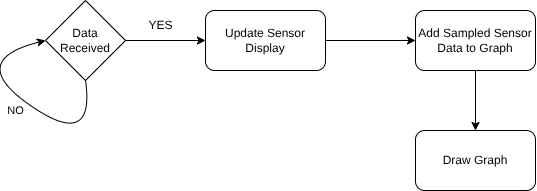
\includegraphics[width=0.7\linewidth]{flow.png}
    \caption{Dataflow of Drawing}
    \label{fig:dataflow}
\end{figure}

The GUI is designed with simplicity in mind. The workflow illustrated above is briefly 
explained as follows. First, the receive thread blocks until data are received from the 
server, which in this case is the Zynq platform. After a data packet is received, the 
sensor display is updated and the data are parsed based on their sensor IDs. The parsed 
sensor data, along with their timestamps, are then added to the graph data structure. 
Finally, all collected data are rendered in the graph.

In the GUI implementation, one critical aspect is the handling of the x-axis timing. 
The GUI must be able to adjust the time window according to user requirements. 
For example, a user may want to view a narrower or wider time window depending on the 
signal being examined. Another important aspect is displaying the most recently sampled 
sensor data within the selected time window. The time window interval is controlled by a 
global variable that can be adjusted at run-time by GUI.

At most, two signals can be drawn in the GUI. Each signal structure consists of several 
attributes: a data point array, a count value, a sensor ID, and minimum and maximum 
values. In the following subsections, the purpose of these attributes is explained in 
detail, with particular emphasis on the minimum and maximum values, since a normalization 
method is applied on the y-axis.

\subsubsection{Update Sensor Display API}

Each sensor sample is first passed to this API, where essential sample details are 
stored in the GUI data structures. Sensors are parsed based on their IDs, after which 
sample details such as the value, timestamp, and sensor ID are assigned to the 
corresponding GUI structures.

After parsing, the GUI is also capable of displaying sensor values and timestamps as 
raw text. Since only two graphs are available, the user may want to view the values of 
additional sensors in textual form. It is important to note that the number of sensors 
may be higher. Finally, the system checks whether the parsed data correspond to the 
currently selected graphs; if so, the \text{add\_graph\_data\_point()}  API is invoked to add the 
parsed data point to the graph.

The \text{add\_graph\_data\_point()} API is explained in the next subsection. The 
following Listing \ref{lst:update_sensor_display} illustrates the implementation of \text{update\_sensor\_display} API.


\begin{lstlisting}[language=C,
caption={Sensor Update Implementation},
label={lst:update_sensor_display}, ]

gboolean update_sensor_display(gpointer data)
{
    sensor_data_update *update = (sensor_data_update *)data;

    if (update == NULL) {
        log_error("update_sensor_display: NULL pointer");
        return FALSE;
    }

    if (update->sid > 5) {
        log_error("Invalid sensor ID: %d", update->sid);
        g_free(update);
        return FALSE;
    }

    char buffer[256];
    int needs_redraw = 0;

    pthread_mutex_lock(&ctx.display_mutex);

    switch (update->sid) {
		case SENSOR_TEMP: {
			uint64_t relative_ms = (update->ts - ctx.start_time) / 1000;

			ctx.display_temp = update->svalue;
			ctx.display_temp_ts = relative_ms;

			snprintf(buffer, sizeof(buffer), "%u", update->svalue);
			gtk_label_set_text(GTK_LABEL(ctx.label_temp), buffer);

			snprintf(buffer, sizeof(buffer), "%" PRIu64 " ms", relative_ms);
			gtk_label_set_text(GTK_LABEL(ctx.label_temp_ts), buffer);

			log_debug("TEMP: %u @ %" PRIu64 " us (relative: %" PRIu64 " ms)",
					 update->svalue, update->ts, relative_ms);

			if (ctx.current_sensor1 == SENSOR_TEMP)
				add_graph_data_point(SENSOR_TEMP, update->svalue, update->ts, 0);
			if (ctx.current_sensor2 == SENSOR_TEMP)
				add_graph_data_point(SENSOR_TEMP, update->svalue, update->ts, 1);
			needs_redraw = 1;
			break;
		}

		case SENSOR_ADC0: {
			uint64_t relative_ms = (update->ts - ctx.start_time) / 1000;

			ctx.display_adc0 = update->svalue;
			ctx.display_adc0_ts = relative_ms;

			snprintf(buffer, sizeof(buffer), "%u", update->svalue);
			gtk_label_set_text(GTK_LABEL(ctx.label_adc0), buffer);

			snprintf(buffer, sizeof(buffer), "%" PRIu64 " ms", relative_ms);
			gtk_label_set_text(GTK_LABEL(ctx.label_adc0_ts), buffer);

			log_debug("ADC0: %u @ %" PRIu64 " us (relative: %" PRIu64 " ms)",
					 update->svalue, update->ts, relative_ms);


			if (ctx.current_sensor1 == SENSOR_ADC0)
				add_graph_data_point(SENSOR_ADC0, update->svalue, update->ts, 0);
			if (ctx.current_sensor2 == SENSOR_ADC0)
				add_graph_data_point(SENSOR_ADC0, update->svalue, update->ts, 1);
			needs_redraw = 1;
			break;
		}

		case SENSOR_ADC1: {
			uint64_t relative_ms = (update->ts - ctx.start_time) / 1000;


			ctx.display_adc1 = update->svalue;
			ctx.display_adc1_ts = relative_ms;

			snprintf(buffer, sizeof(buffer), "%u", update->svalue);
			gtk_label_set_text(GTK_LABEL(ctx.label_adc1), buffer);

			snprintf(buffer, sizeof(buffer), "%" PRIu64 " ms", relative_ms);
			gtk_label_set_text(GTK_LABEL(ctx.label_adc1_ts), buffer);

			log_debug("ADC1: %u @ %" PRIu64 " us (relative: %" PRIu64 " ms)",
					 update->svalue, update->ts, relative_ms);


			if (ctx.current_sensor1 == SENSOR_ADC1)
				add_graph_data_point(SENSOR_ADC1, update->svalue, update->ts, 0);
			if (ctx.current_sensor2 == SENSOR_ADC1)
				add_graph_data_point(SENSOR_ADC1, update->svalue, update->ts, 1);
			needs_redraw = 1;
			break;
		}

		case SENSOR_SWBTN:
			if (ctx.display_swbtn != update->svalue) {
				ctx.display_swbtn = update->svalue;

				snprintf(buffer, sizeof(buffer), "0x%02X", update->svalue);
				gtk_label_set_text(GTK_LABEL(ctx.label_switch), buffer);
				log_debug("SWITCH: 0x%02X", update->svalue);

				ctx.display_pushb = (update->svalue >> 8);
				snprintf(buffer, sizeof(buffer), "0x%02X",  (update->svalue >> 8));
				gtk_label_set_text(GTK_LABEL(ctx.label_pushb), buffer);
				log_debug("PUSHB: 0x%02X", update->svalue);

			}
			break;

		default:
			log_error("Unknown sensor ID: %d", update->sid);
			break;
    }

    pthread_mutex_unlock(&ctx.display_mutex);

    g_free(update);

    if (needs_redraw && ctx.drawing_area != NULL) {
        gtk_widget_queue_draw(ctx.drawing_area);
    }

    return FALSE;
}

\end{lstlisting}


\subsubsection{Add Sampled Sensor Data to Graph API}

The main responsibility of the \text{add\_graph\_data\_point()} API is to receive sampled data and 
add it to the graph structure. While doing so, it also removes any samples that fall 
outside the current time window interval. Implementing the addition of only those samples 
within the time window is straightforward. First, the API checks whether the timestamp of 
the current sample exceeds the sliding window threshold; if so, it updates the start of 
the time window accordingly. After updating the time window, it scans the buffer for any 
samples that are older than the time window and removes them. Finally, the count variable 
in the graph structure is updated, and the sensor values are stored in the graph structure.

At the end of the API, the minimum and maximum sensor values are updated. This is 
necessary because a normalization method is applied to the y-axis, and these values are 
required for proper scaling. Listing \ref{lst:adddata} presents the complete implementation of the API.


\begin{lstlisting}[language=C,
caption={Add Sampled Sensor Data to Graph Implementation},
label={lst:adddata}, ]
void add_graph_data_point(uint32_t sensor_id, uint32_t raw_value, uint64_t timestamp, int graph_index)
{
	/* Get sensor graph data struct as pointer*/
	sensor_graph_data *g = &ctx.graph_data[graph_index];

    pthread_mutex_lock(&ctx.graph_mutex);
    /* Convert raw to unit data*/
    double value = convert_raw_to_unit(sensor_id, raw_value);


    uint64_t window_start = 0;
    uint32_t write = 0;

    /* Are these points older than our timing window? if older, filter it*/
    if (timestamp > SLIDING_WINDOW_US)
    {
    	/* Is time now greater then window time interval ? */
    	window_start = timestamp - SLIDING_WINDOW_US;

        for (int i = 0; i < g->count; i++)
        {
            if (g->points[i].timestamp >= window_start)
            {
                g->points[write++] = g->points[i];
            }
        }
        /* Our new count value since we added some of them to beginning*/
        g->count = write;
    }

    /* Add new data point to buffer */
    if (g->count < MAX_DATA_POINTS)
    {
         g->points[g->count].timestamp = timestamp;
         g->points[g->count].value = value;
         g->count++;
     }

    /* Update new minimum and maximum values*/
    if (g->count == 1)
    {
        g->min_val  = value;
        g->max_val  = value;
    } else
    {
        if (value < g->min_val)
        					g->min_val = value;
        if (value > g->max_val)
        					g->max_val = value;
    }

    pthread_mutex_unlock(&ctx.graph_mutex);
}
\end{lstlisting}


\subsubsection{Draw Graph API}
The \text{on\_draw\_graph()} API is responsible for rendering the graph in the GUI. It first 
retrieves the size of the drawing area and exits if the dimensions are invalid. To ensure 
thread-safe access, it locks the graph data with a mutex. The background of the graph 
area is filled with white to create a clean canvas. If there is no data in either graph 
buffer, a placeholder message “No data to display” is shown, and the function exits after 
releasing the mutex.

The usable plotting area is calculated by subtracting margins from the widget dimensions. 
The minimum and maximum values of each graph are retrieved and adjusted with a small 
padding to avoid drawing at the edges. One of the most important aspects of this API is 
the handling of timing for the x-axis. The API implements a sliding time window, which 
determines the portion of the data that is visible on the graph. The start of the visible 
time range is calculated based on the timestamp of the latest sampled data. Only data 
points within this time window are drawn, ensuring that the graphs always display the most 
recent and relevant information. This approach allows the GUI to dynamically update in 
real time while providing a consistent view of the signal over a fixed duration.

After setting general plot configurations, the two graphs are drawn using their respective 
data and axes ranges. Labels for the y-axis and x-axis are added to indicate values and 
time intervals, and graph titles are displayed to provide context. Finally, the mutex is 
released, completing the drawing process. By carefully managing the timing and applying 
the sliding window, the GUI ensures that users see up-to-date graph data in a visually 
organized and real-time manner.

Listing \ref{lst:draw} presents the complete implementation of the drawing API.

\begin{lstlisting}[language=C,
caption={Graph Draw API},
label={lst:draw}, ]

gboolean on_draw_graph(GtkWidget *widget, cairo_t *cr, gpointer data)
{
	/* Get Info on size of GUI*/
    int width = gtk_widget_get_allocated_width(widget);
    int height = gtk_widget_get_allocated_height(widget);

    if (width <= 0 || height <= 0)
        					return FALSE;

    pthread_mutex_lock(&ctx.graph_mutex);

    /* Draw the background of GUI */
    cairo_set_source_rgb(cr, 1, 1, 1); /* White color */
    cairo_rectangle(cr, 0, 0, width, height);
    cairo_fill(cr);

    /* If there is no data, write text that no data in buffer! */
    if (ctx.graph_data[0].count == 0 && ctx.graph_data[1].count == 0)
    {
        cairo_set_source_rgb(cr, 0.5, 0.5, 0.5);
        cairo_select_font_face(cr, "Monospace",
                               CAIRO_FONT_SLANT_NORMAL,
                               CAIRO_FONT_WEIGHT_NORMAL);
        cairo_set_font_size(cr, 14);
        cairo_move_to(cr, width / 2 - 80, height / 2);
        cairo_show_text(cr, "No data to display");
        pthread_mutex_unlock(&ctx.graph_mutex);
        return FALSE;
    }

    /* Calculate graph area that we can use*/
    int graph_width = width - margin_left - margin_right;
    int graph_height = height - margin_top - margin_bottom;
    /* Check if it is correct */
    if (graph_width <= 0 || graph_height <= 0)
    {
        pthread_mutex_unlock(&ctx.graph_mutex);
        return FALSE;
    }

    /* Get min and max val for Graphs */
    double min_val1 = ctx.graph_data[0].min_val;
    double max_val1 = ctx.graph_data[0].max_val;
    double min_val2 = ctx.graph_data[1].min_val;
    double max_val2 = ctx.graph_data[1].max_val;

    /* Calculate the range of Y-axis for Graph1*/
    double range1 = (max_val1 > min_val1) ? (max_val1 - min_val1) : 1;
    /* Add padding to Y-axis*/
    uint32_t pad1 = (range1 / 10) + 1;
    /* Calculate new min-max with paddings*/
    min_val1 = (min_val1 > pad1) ? (min_val1 - pad1) : 0;
    max_val1 += pad1;

    /* Calculate the range of Y-axis for Graph2*/
    uint32_t range2 = (max_val2 > min_val2) ? (max_val2 - min_val2) : 1;
    /* Add padding to Y-axis*/
    uint32_t pad2 = (range2 / 10) + 1;
    /* Calculate new min-max with paddings*/
    min_val2 = (min_val2 > pad2) ? (min_val2 - pad2) : 0;
    max_val2 += pad2;

    /* Sliding timing window implementation*/
    uint64_t now = latestSampledTime();

    /* Set min-time */
    uint64_t min_time = (now > SLIDING_WINDOW_US)
                        ? (now - SLIDING_WINDOW_US)
                        : 0;

    uint64_t time_range = SLIDING_WINDOW_US;

    /* Settings of graph and grid lines */
    plotSettings(cr , graph_height , graph_width);

    /* Configuration for Graph-1 */
    plotGraph1 (cr, min_time , time_range , graph_width ,
    					graph_height ,min_val1 , max_val1);


    plotGraph2 (cr , min_time, time_range ,graph_width,
    					graph_height , min_val2, max_val2);

	/* Labeling to Y-Axis */
    //plotLabelYaxis (cr , graph_height , min_val1 , max_val1);
    plotDualYAxis (cr , graph_height ,graph_width ,  min_val1 , max_val1
    				, min_val2 , max_val2);

	/* Labeling to X-Axis */
    plotLabelXaxis (cr , graph_width , graph_height , min_time , time_range);

    /* Axis titles */
    plotTitles(cr , width , height);

    pthread_mutex_unlock(&ctx.graph_mutex);
    return FALSE;
}

\end{lstlisting}



\subsection{GUI Related Requirement Analysis}
This section analyzes the graphical user interface (GUI) related requirements of the 
project and explains how the proposed GUI design and implementation satisfy these 
requirements. Each requirement is evaluated individually, with emphasis on usability, 
layout, user interaction, and responsiveness. The corresponding design choices, interface 
components, and implementation details are discussed. The objective of this analysis is to 
demonstrate that the developed GUI meets the functional, usability, performance, and 
reliability requirements defined at the beginning of the project, while providing a clear 
and intuitive user experience.

\subsubsection{Functional Requirements}
\label{subsubsection:funcreq}

\begin{tcolorbox}[
    title=REQ-9,
    colback=gray!5,
    colframe=gray,
    fonttitle=\bfseries
]
The Control/Monitor program (GUI) shall configure which sensors should acquire data.
\end{tcolorbox}

\paragraph{REQ-9 Analysis and GUI Mapping}\

The GUI provides frequency configuration controls that allow the user to set the 
sampling frequency for each sensor individually. By setting a sensor’s frequency to 0 Hz, 
the corresponding sensor is disabled and stops acquiring data. This requirement is 
satisfied through the implementation of per-sensor frequency configuration within the GUI. 
The functionality can be verified both on real hardware and within a test environment, 
confirming that sensors correctly start or stop data acquisition based on the configured 
frequency.

\begin{tcolorbox}[
    title=REQ-10,
    colback=gray!5,
    colframe=gray,
    fonttitle=\bfseries
]
The Control/Monitor program (GUI) shall configure a sampling rate for each sensor.
\end{tcolorbox}

\paragraph{REQ-10 Analysis and GUI Mapping}\

The GUI allows the user to configure the sampling rate for each sensor by adjusting its 
frequency in the interface. The selected frequency is applied by sending a command to the 
server side, where the command parameters specify which sensor to configure and the 
desired frequency. The server parses these commands through its API and executes the 
corresponding action for the specified sensor. This requirement is verified through
testing on real hardware as well as within a controlled test environment, and further 
details can be investigated by referring to the software development report.


\begin{tcolorbox}[
    title=REQ-11,
    colback=gray!5,
    colframe=gray,
    fonttitle=\bfseries
]

The Control/Monitor program (GUI) shall display live sensor data in text form.
\end{tcolorbox}

\paragraph{REQ-11 Analysis and GUI Mapping}\
The GUI displays live sensor data in text form, positioned on the left side of the 
interface for clear visibility. This functionality is implemented in the 
\text{update\_sensor\_display()} API which can be seen in Listing \ref{lst:update_sensor_display}, which updates the textual display before adding the sensor 
data to the graphical display. This requirement is verified through testing on real 
hardware as well as within a controlled test environment, ensuring that sensor data is 
accurately and consistently displayed in real time.



\begin{tcolorbox}[
    title=REQ-12,
    colback=gray!5,
    colframe=gray,
    fonttitle=\bfseries
]
The Control/Monitor program (GUI) shall display up to 2 signals in a live diagram
\end{tcolorbox}

\paragraph{REQ-12 Analysis and GUI Mapping}\

The GUI displays up to two signals simultaneously in a live graph within the monitor. 
This functionality is implemented in the \text{on\_draw\_graph()} API which can be seen in Listing \ref{lst:draw}. To improve readability and 
visual clarity, the signal values are normalized along the y-axis. This requirement is 
verified through testing on real hardware as well as within a controlled test environment, 
ensuring that up to two signals are accurately displayed in real time.





\subsubsection{Design Requirements}

\begin{tcolorbox}[
    title=REQ-15,
    colback=gray!5,
    colframe=gray,
    fonttitle=\bfseries
]
The GUI shall use GTK C code.
\end{tcolorbox}

\paragraph{REQ-15 Analysis and GUI Mapping}\

The GUI is implemented using the GTK library with the C programming language to ensure 
high performance and efficiency. This implementation choice is discussed in the 
Introduction section, and further details can be found by referring to the relevant 
API documentation presented in this report.


\subsubsection{Test Requirements}

\begin{tcolorbox}[
    title=REQ-26,
    colback=gray!5,
    colframe=gray,
    fonttitle=\bfseries
]
The functional requirents shall be tested by suitable test setups
\end{tcolorbox}

\paragraph{REQ-26 Analysis and GUI Mapping}\

The GUI is tested using multiple test setups to verify all functional attributes of the 
interface. As described in \cref{subsection:asd}, the server is implemented within a Linux-based 
test environment, allowing comprehensive testing of the GUI under various operating 
conditions. All GUI functionalities are verified across different test cases, and the 
corresponding test results are presented in the referenced section.


\subsection{Test and Verification of GUI}
\label{subsection:asd}
This section describes the test and verification process used to validate the 
functionality of the GUI requirements. A Linux-based Ethernet connection is used to 
establish a server on the host machine. Subsequently, test files generating mock 
sensor signals are transmitted to the GUI via the Ethernet interface. This setup enables 
systematic testing and verification of the GUI functionalities under controlled 
conditions. Although it is not feasible to present all possible test cases in this 
section, the most critical and representative cases are discussed.

\subsubsection{Verification of Requirement REQ-11}
First, the overall appearance of the GUI is presented. At this stage, sensor data are 
transmitted from the test environment, and two live graphs are displayed within the GUI.


\begin{figure}[H]
    \centering
    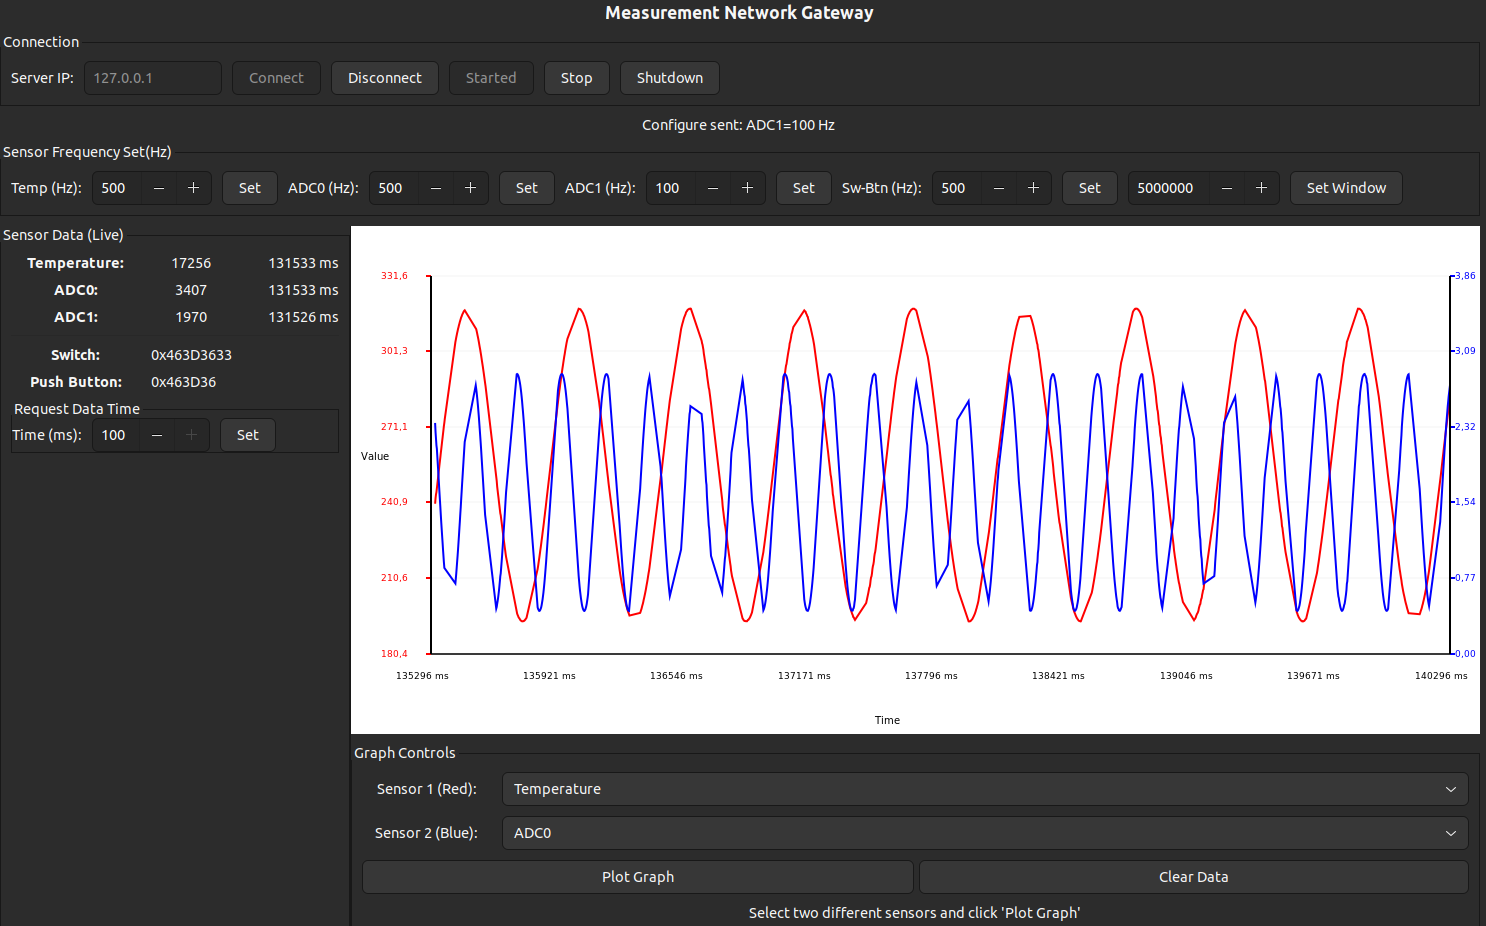
\includegraphics[width=0.8\linewidth]{gui.png}
    \caption{GUI}
    \label{fig:gui}
\end{figure}

First, \cref{fig:gui} is explained. As shown on the left side of the interface, all 
sensor data are displayed in live textual form. Based on this observation, REQ-11 in \cref{subsubsection:funcreq} is verified.

\subsubsection{Verification of Requirement REQ-10}
Secondly, as shown by the sensor frequency configuration row in the upper part of the GUI, 
the sampling frequencies of the sensors can be configured. To verify this functionality, 
the temperature sensor frequency is modified. In Figure \ref{fig:gui}, the temperature sensor operates 
at 500 Hz; this frequency is changed to 10 Hz to examine the resulting signal behavior.

\begin{figure}[H]
    \centering
    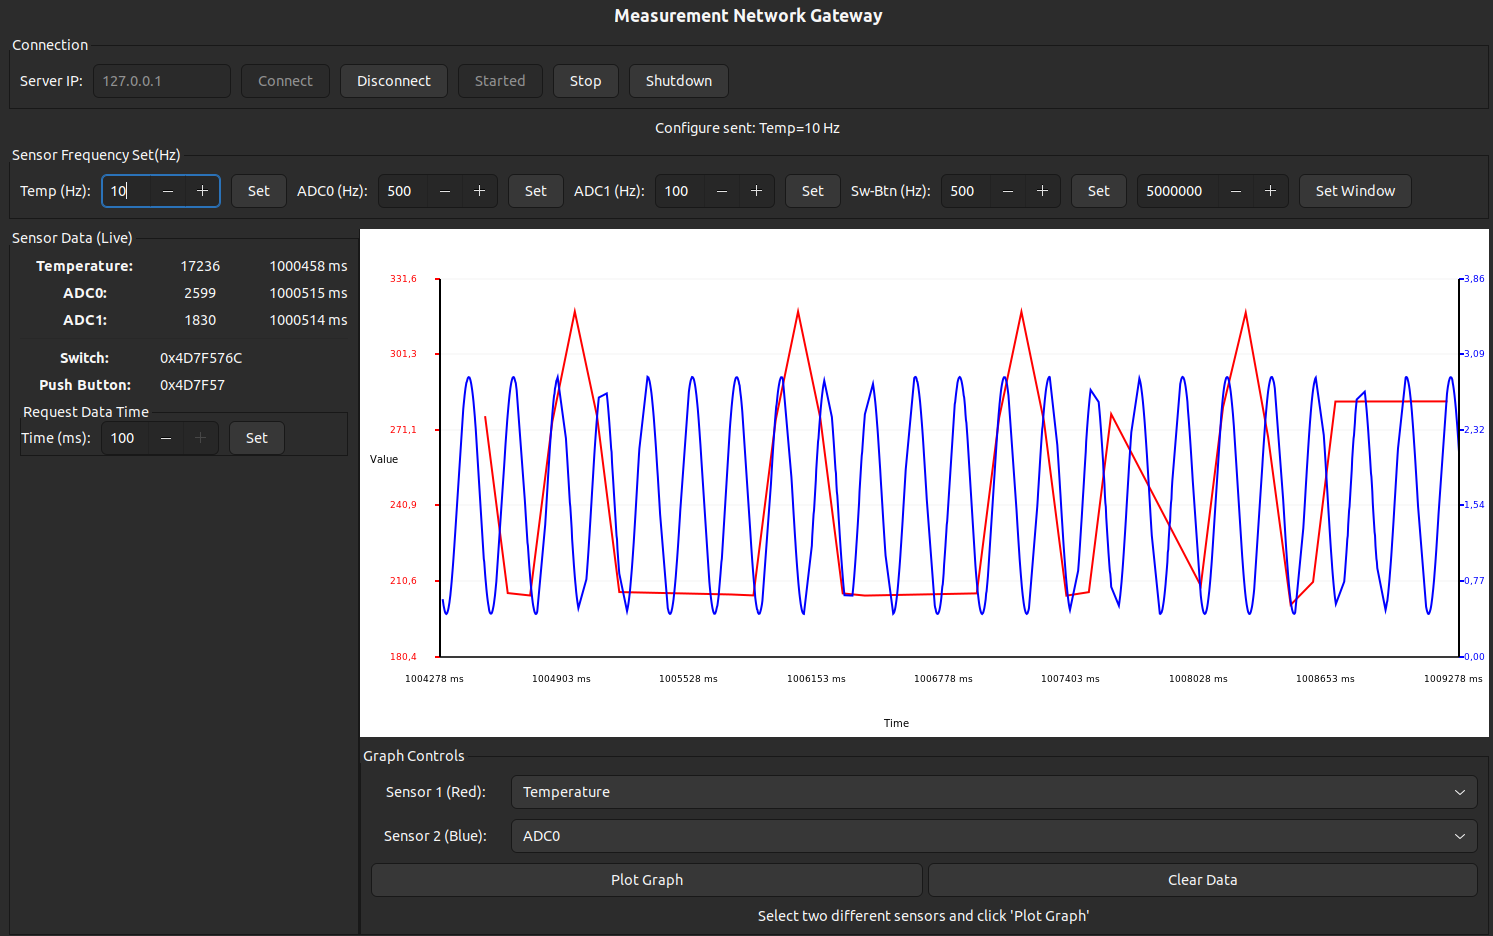
\includegraphics[width=0.8\linewidth]{freqchang.png}
    \caption{Frequency Settings Effect to Signal}
    \label{fig:frecch}
\end{figure}

As shown in Figure \ref{fig:frecch} above, the signal quality of the temperature signal is significantly 
reduced. This observation demonstrates that the sampling frequency configuration 
functions as intended; therefore, Requirement REQ-10 is met, as described in Section \ref{subsubsection:funcreq}.

\subsubsection{Verification of Requirement REQ-9}
In addition, sensor sampling can be stopped by setting the corresponding frequency to 0 Hz. 
This functionality corresponds to Requirement REQ-9 described in Section \ref{subsubsection:funcreq}. As shown in 
Figure \ref{fig:zerofreq}, when the ADC0 sensor frequency is set to 0 Hz, the sensor stops sampling and no 
data are displayed. Based on this observation, Requirement REQ-9 is met.

\begin{figure}[H]
    \centering
    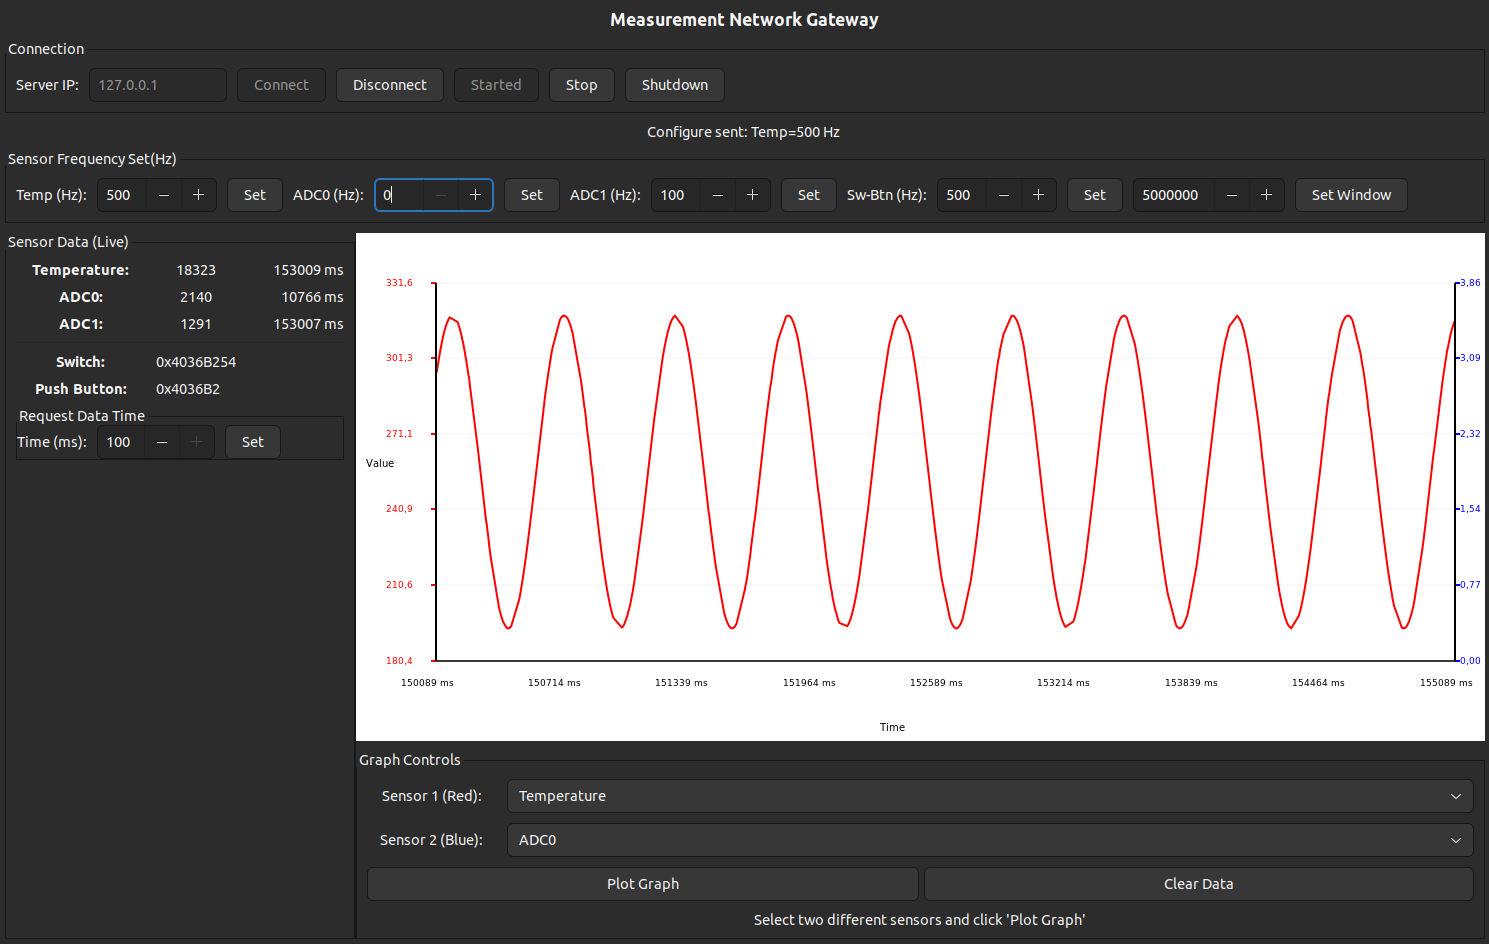
\includegraphics[width=0.8\linewidth]{zerfreq.png}
    \caption{Zero Frequency Settings Effect to Signal}
    \label{fig:zerofreq}
\end{figure}

\subsubsection{Verification of Requirement REQ-12}
Requirement REQ-12, which specifies the display of up to two signals in a live diagram, 
is demonstrated by the figures shown above. Additionally, the user can switch between 
different signals by selecting the desired sensors in the graph control section of the GUI. 
Based on these observations, Requirement REQ-12, as defined in Section \ref{subsubsection:funcreq}, is met.

\begin{figure}[H]
    \centering
    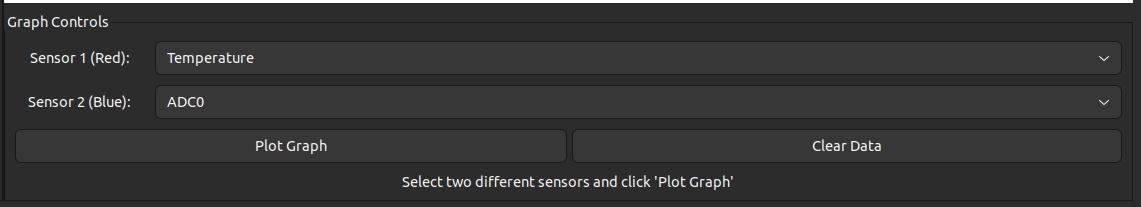
\includegraphics[width=0.8\linewidth]{graphcontrol.png}
    \caption{Graph Control for Live Signals}
    \label{fig:graph}
\end{figure}

\subsubsection{Verification of Requirement REQ-15}

This requirement is discussed in the Introduction in section \ref{subsection:intro} and illustrated in Listings \ref{lst:update_sensor_display}
\ref{lst:adddata} and \ref{lst:draw}, 
demonstrating how REQ-15 has been met.

\subsubsection{Verification of Requirement REQ-26}

All of the requirements described above have been verified using the test setups. 
This demonstrates that the functional requirements have been thoroughly tested, 
confirming that Requirement REQ-26 in Section \ref{subsubsection:funcreq} is met.

\subsection{Results}

The GUI was thoroughly tested and verified to ensure all functional requirements are met. 
Sensor data are correctly displayed in both textual and graphical forms, with live updates 
reflecting real-time signals. Users can configure sensor sampling frequencies, including 
stopping sensors by setting their frequency to 0 Hz, and switch between signals on the 
live graph as intended. The implementation using the GTK library in C performs efficiently 
and reliably. Test results from real hardware and controlled environments confirm that 
the GUI functions as designed. Overall, the system meets the expected usability, 
performance, and reliability standards.


\clearpage 
\null 
\vfill 
\begin{center}
{\textbf {\large Haizon, Ameer, Alin Application }} 
\end{center}
\vfill 
\thispagestyle{empty}
\clearpage


\clearpage 
\null 
\vfill 
\begin{center}
\textbf{\large Haizon Helet Cruz (42708)}
\end{center}
\vfill 
\fancyhead[L]{MNG Application (Haizon Helet Cruz 42708)}
\clearpage


\chapter{MNG Application Part I}
\section{THREAD SAFE RING BUFFER IMPLEMENTATION}
\subsection{Introduction}
The ring buffer or circular queue, is a storage mechanism designed to manage continuous streams of data within a fixed-memory footprint. This is unlike a linear queue which requires memory shifts or reallocation of elements are added and removed, a ring buffer connects its end back to its beginning. The choice of ring buffer, to be used in this project is fairly self explanatory, it is a very efficient operation particularly the enqueue and dequeue operations are performed in O(1) constant time, ensuring that the system’s throughput remains deterministic regardless of how much data has already been processed. 

In the context of Measurement Network Gateway, the ring buffer acts as a vital asynchronous bridge between two decoupled threads: the sensor data acquisition thread and network transmission thread. These threads are totally independent and without an appropriate storage mechanism will lead to catastrophic data loss. With the use of a ring buffer, the producer can “fire and forget” its data, while the consumer drains that data in optimized batches whenever the communication channel is ready. By encapsulating this logic with POSIX mutexes, the ring buffer ensures that even if both threads attempt to access the indices at the exact same time even down to a microsecond precision, its internal state remains consistent and memory-safe.

\subsection{ARCHITECTURAL ROLE IN MNG}
In the broader scope of the MNG architecture, the ring buffer serves as a temporal isolation layer, a critical bridge that decouples two threads with fundamentally incompatible timing characteristics. On the production side, the sensor acquisition thread operates within a hard real-time domain, requiring high-frequency, deterministic periodic sampling. This thread cannot afford to block or wait, as any delay would immediately violate real-time guarantees and destabilize the data’s temporal integrity. Conversely, the network streaming thread exists in an asynchronous, non-deterministic domain where it is subject to the unpredictable nature of TCP/IP congestion, signal jitter, and packet retransmissions.

Without the ring buffer acting as a mediator, the sensor task would be forced to inherit the network’s timing variability. If the network stalled, the sensor task would stall, leading to catastrophic failure in control loops. By implementing this module, the architecture enforces temporal decoupling, allowing the sensor thread to maintain its rigid sampling schedule regardless of the network's current state. The buffer effectively provides backpressure absorption, acting as a shock absorber that stores data during bursts of network congestion and drains it when bandwidth becomes available.

Ultimately, this design ensures a producer non-blocking guarantee. The sensor task can "fire and forget" its samples into the buffer with the assurance that the operation will always complete in O(1) time. This architectural role is finalized by ensuring data coherency under concurrency, where the mutex-protected FIFO queue allows these two disparate timing domains to exchange information safely. By transforming a chaotic, non-deterministic network demand into a structured, bounded memory operation, the ring buffer ensures the overall system remains stable, responsive, and accurate.

\subsection{DATA STRUCTURE DESIGN }
This section defines important factors considered during the implementation process of the said ring buffer:\\

\subsubsection*{Memory Determinism}
The ringBuffer was declared using the following piece of code referenced in \texttt{mainH.h}.
\begin{minted}[bgcolor = lightgray, tabsize = 4, breaklines]{c}
extern ring_buffer_t *rb;
\end{minted}

and its implementation was completed in \texttt{ringBuffer.c} and initialized in \texttt{main.c}.


\begin{figure}[H]
\centering 
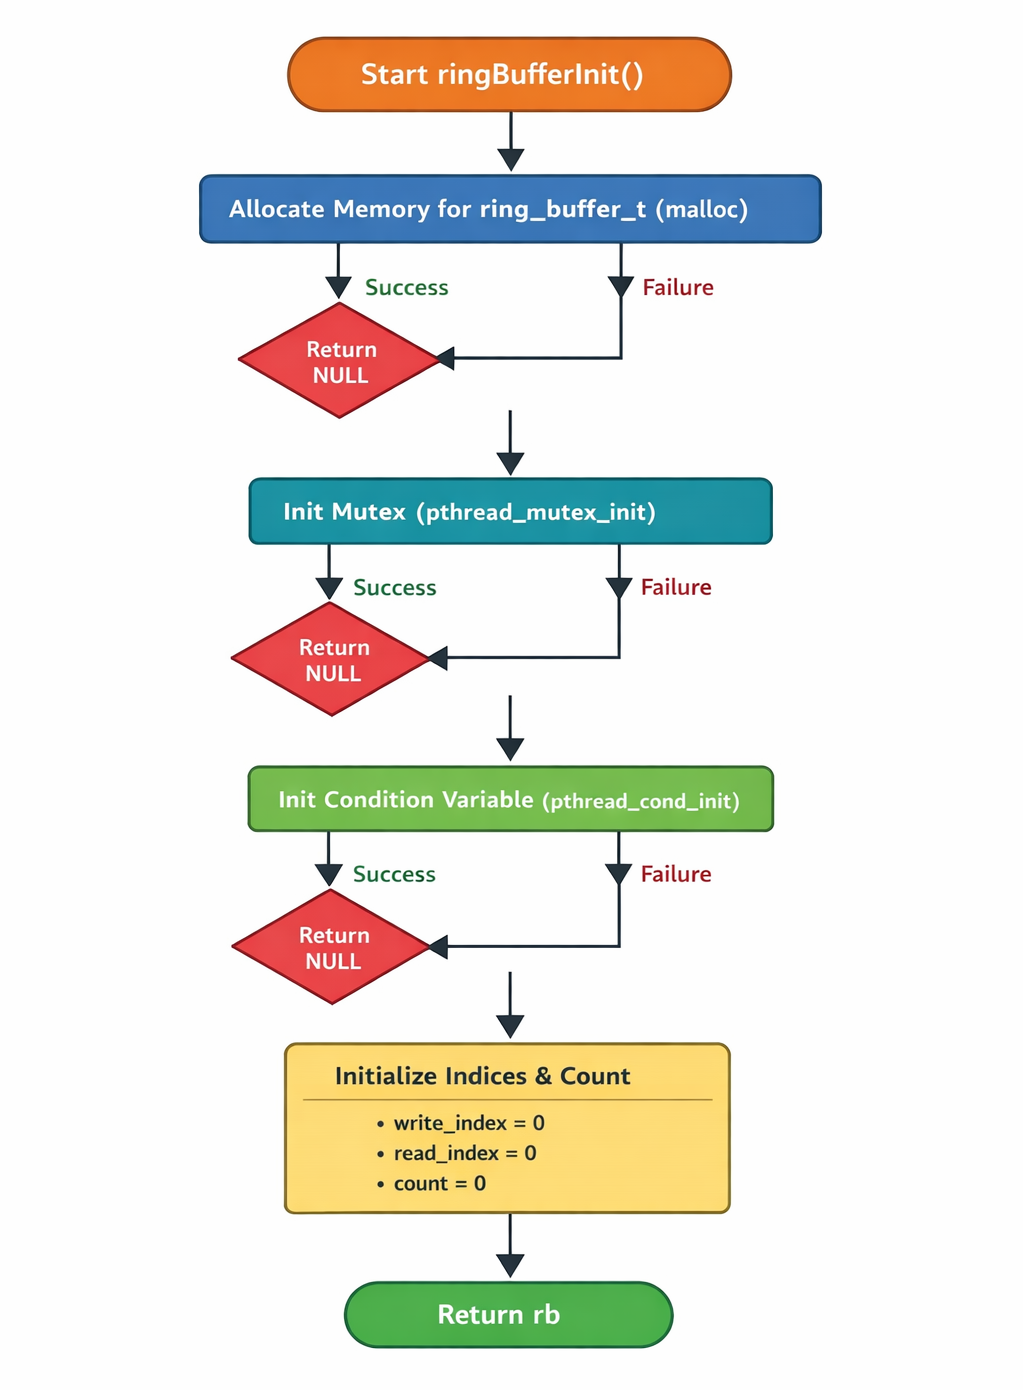
\includegraphics[scale = 0.35]{media/haizangui4.png}
\caption{Ring Buffer Data Init}
\label{fig-haizangui1}
\end{figure}

\clearpage 
\subsubsection*{Indexing Model}
The ring buffer type is defined using the following structure:

\begin{minted}[bgcolor = lightgray, tabsize = 4, breaklines]{c}
typedef struct ring_buffer
{
    pthread_mutex_t rbMutex;
    sensor_data_t sampleArray[RING_BUF_SIZE];
    size_t write_index;
    size_t read_index;
    uint16_t count;
    pthread_cond_t  data_available;
} ring_buffer_t;
\end{minted}
In the architecture of a circular buffer, the management of the \texttt{read\_index} and \texttt{write\_index} through modulo arithmetic is what enables the structure to simulate an infinite loop within a finite static memory block. By calculating the next position as \texttt{(index + 1)(mod N)}, the logic ensures that once the end of the buffer is reached, the pointer automatically wraps back to the zero-th index. This mathematical constraint is the key to the buffer’s O(1) efficiency.

Another logical challenge arises when using only \texttt{read\_index} and \texttt{write\_index} to determine the state of the buffer. In the implementation it becomes naive when the condition where \texttt{read\_index} and \texttt{write\_index} becomes equal, as the identical state occurs when the buffer is entirely empty and when it has been filled to its maximum capacity. To remove this ambiguity, we can use another variable named count. By maintaining a real time data count of the samples stored, the implementation can immediately disambiguate these states: if states are equal and the count is zero, the consumer knows there is nothing to process, whereas if they are equal and the count is N, the producer knows that the buffer is full and it must begin the overwrite procedure.

\subsection{Concurrency Model}
The concurrency model of the ring buffer is built upon the interaction between a producer thread, responsible for high-frequency sensor acquisition, and a consumer thread, which handles the non-deterministic timing of network transmissions. Because these two tasks operate asynchronously, they must access the same memory addresses for the sampleArray, indices, and count variable. This shared access necessitates the use of a POSIX mutex to enforce mutual exclusion, ensuring that only one thread can modify or evaluate the buffer’s internal state at any given microsecond. Without this lock, a race condition is nothing but certain when the producer updates the write\_index at the exact moment the consumer is attempting to read it, leading to “memory tearing” or a corrupted value of count.

Beyond simple mutual exclusion, the implementation utilizes a condition variable, data\_available, to manage the lifecycle of the consumer thread efficiently. Without such an implementation the consumer might “busy-wait”, constantly polling the buffer in a tight loop to see if new data has arrived, which needlessly consumes CPU cycles and increases power consumption. By integrating this condition, the consumer can instead enter a suspended state, relinquishing the processor until the producer explicitly signals that new data is ready. This transition from a “polling” model to a “signaled” model drastically reduces system overhead and ensures that the network task reacts with minimal latency the moment a sensor sample is successfully stored.

 In extension, the buffer following an overflow policy refers to the implementation decision to drop the oldest sample when the buffer reaches its maximum capacity, tailored for real-time telemetry systems. By advancing the read index in tandem with the write index during an overflow, the system effectively slides the window of available data forward. This ensures that the producer never encounters a block or wait state. In a streaming context, this non-blocking behavior is paramount; if the producer were forced to wait for a slow network consumer, the resulting sampling jitter would destabilize high-frequency control loops and cause the system’s real-time guarantees to collapse entirely.

\subsection{Insert Operation}
The insertion operation or addition of samples to the ring buffer is carried out using the function\\
\texttt{ringBufferAddSample} in \texttt{ringBuffer.c.}

The addition operation follows a strict, sequential protocol designed to maintain the integrity of the shared state while ensuring that the producer thread never experiences non-deterministic delays. By immediately acquiring the \texttt{rbMutex}, the function creates a protected critical section where the pointer arithmetic and the data write can occur without interference from the consumer thread. Once the \texttt{sensor\_data\_t }payload is copied into the sampleArray at current \texttt{write\_index}, the index is incremented using modulo arithmetic to facilitate the circular wrap-around.

The insertion logic rather than failing or blocking when the buffer is full, the function performs a conditional check on the count. If the ring buffer has reached \texttt{RING\_BUF\_SIZE}, the \texttt{read\_index} is manually advanced to the next position. This ensures that the \texttt{FIFO (First-IN-First-OUT)} order is preserved by effectively evicting the oldest sample to make room for the newest. Following the update of the indices and the count,  the function issues a \texttt{pthread\_cond\_signal} to the \texttt{data\_available} condition variable. This signal is essential for system efficiency, as it alerts any sleeping consumer thread that the buffer is no longer empty, transitioning the consumer from a suspended state back to an active processing state.

From a performance standpoint, the insertion operation is characterized by its O(1) constant time complexity. Because the implementation avoids heap interaction, dynamic resizing, or complex memory copying, the execution time remains identical whether the ring buffer is empty or nearly full. The lack of malloc or calloc calls within the write path is necessary for high-frequency sampling, as it eliminates the risk of non-deterministic latencies caused by memory management overhead or heap fragmentation. This makes the write path exceptionally reliable for real-time sensor tasks where every microsecond of jitter can impact the accuracy of the resulting data stream.

\subsection{Batch Extraction}
The extraction of samples in batch by the consumer or the network thread is done using the function \texttt{ringBufferRemoveBatch} in \texttt{ringBuffer.c}.

This function represents a critical performance optimization layer, moving beyond simple data retrieval to address the systemic overhead of concurrent execution. In a high-frequency environment, the cost of synchronization can often exceed the cost of data movement itself. Without a batching mechanism, extracting 100 samples would required 100 individual calls to a single-removal function, triggering 100 discrete lock and unlock cycles. Each cycle presents a fresh opportunity for the OS scheduler to perform a context switch, increasing the likelihood of mutex contention and causing significant cache invalidation as the processor repeatedly arbitrates into a single critical section, locking the mutex once to perform a linear memory transfer before releasing it.

Batching aligns perfectly with the requirements of network protocols. Since network hardware and TCP stacks operate most efficiently when handling larger payloads, the ability to drain the buffer in blocks allows the system to maximize packet utilization. This reduces the relative overhead of headers and improves overall bandwidth efficiency, ensuring that the network gateway remains a high-throughput conduit rather than a bottleneck. The function also ensures that the \texttt{read\_index} and count are updated in a single cohesive block after the target number of samples has been reached. This approach not only preserves the data structure invariants but also provides a deterministic execution path that is highly friendly to modern CPU instruction pipelining. In this gateway project, where sensor samples are processed fast, this batching strategy is not merely a convenience but a mandatory requirement for system stability. It transforms the read path into a high-speed data drain, ensuring the consumer can keep pace with a prolific producer while maintaining the lowest possible CPU overhead.

\begin{figure}[H]
\centering 
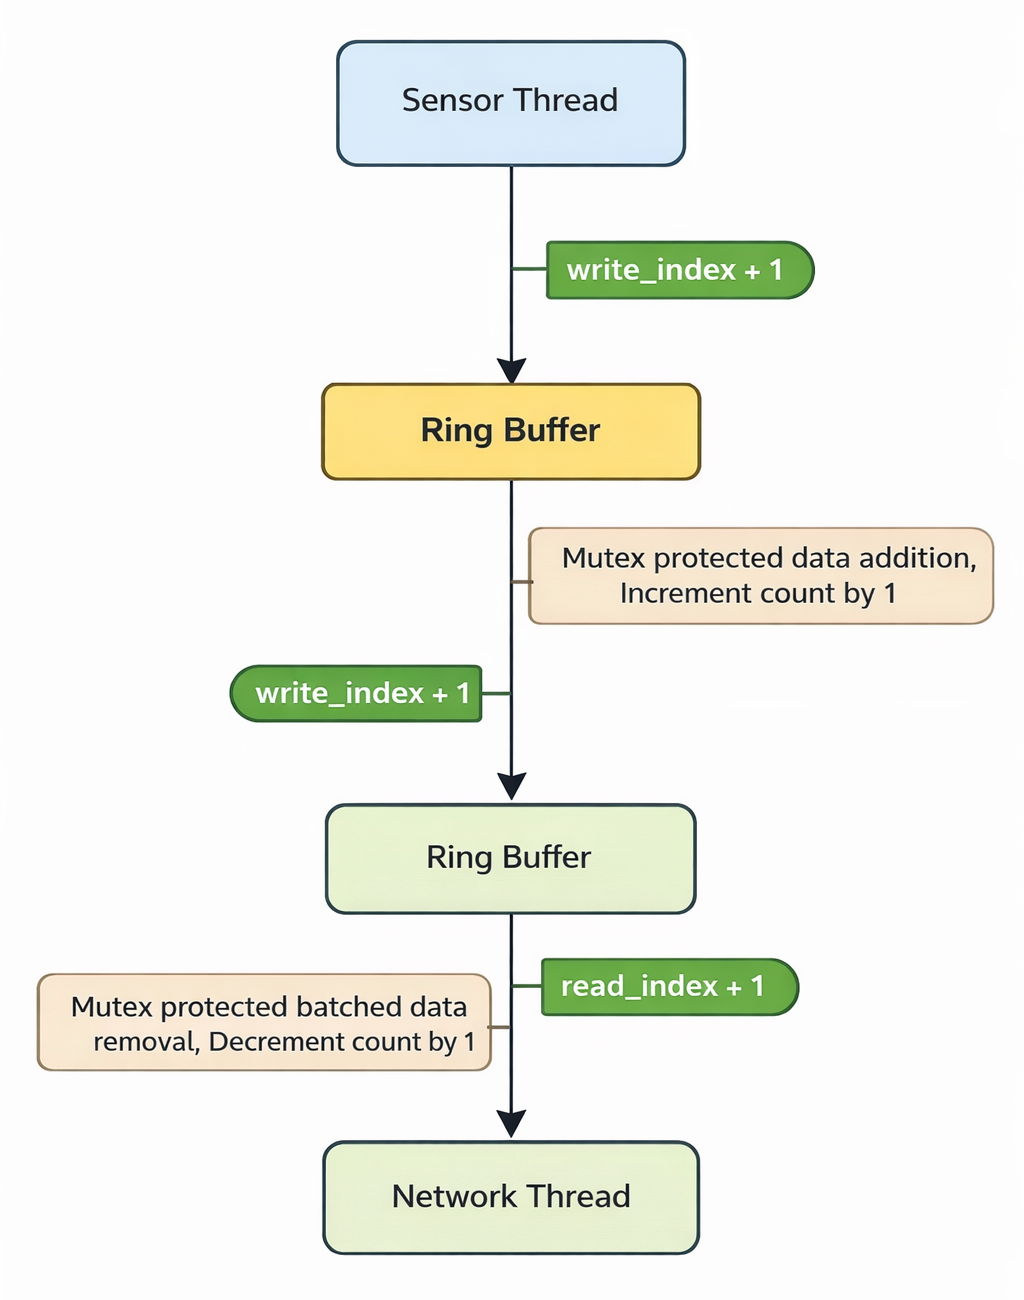
\includegraphics[scale = 0.24]{media/haizangui5.png}
\caption{Ring Buffer Data Flow}
\label{fig-haizangui2}
\end{figure}

\subsection{Complexity Analysis}
The efficiency of a ring buffer is best understood through a formal complexity analysis, which confirms that the design has reached the theoretical limit for queue based operations. Every core function-initialization, insertion, and both single and batch removal-operates within a deterministic time frame, regardless of the gateway’s uptime or the volume of data processed.

When the buffer is empty or requires an overwrite of the oldest sample, the operation involves a fixed number of index increments and a single memory copy which ensures O(1) complexity, while the batch remove function iterates through k samples, its complexity is technically O(k), however in the context of the data structure’s overhead, it remains optimal because it performs the minimum necessary work (one copy per element) while reducing the synchronization cost to O(1) per batch rather than O(k).

The space complexity of the insert method is O(N), where N is the \texttt{RING\_BUF\_SIZE}. This is the most efficient use of memory possible for a buffer, as it allocates exactly enough space for the required data without any hidden pointers, metadata nodes, or dynamic overhead associated with linked-list implementations. Because the memory is statically defined within the \texttt{ring\_buffer\_t} struct, the system’s memory footprint is entirely predictable at compile-time, which is a prerequisite for safety-critical embedded applications.

Beyond the standard Big O notation, the implementation is optimized for real-time determinism. By avoiding heap-based functions like malloc() and free() during the write and read paths, the code eliminates the risk of “Long-Tail latency” caused by memory fragmentation or garbage collection cycles. The use of a single mutex ensures that while the threads are synchronized, the “lock-time” remains minimal and constant. This makes the ring buffer an “optimal” bridge: it provides the highest possible throughput with the lowest possible jitter, satisfying the rigorous timing constraints of high-frequency sensor acquisition and network streaming.

\begin{table}[H]
    \centering 
        \begin{tabular}{lll}
        \toprule
		\textbf{Operation} & \textbf{Time Complexity} & \textbf{Space Complexity} \\
		\midrule 
		Insert & $O(1)$ & $O(N)$ fixed \\
		Batch Remove &  $O(k)$ & $O(1)$ \\
        \bottomrule
    \end{tabular}
\end{table}

where: \\
N = 2048, \\
K = number of samples extracted in a batch. \\

The size of the ring buffer was decided on the following calculation\\
Max sampling rate = 1kHz, and a network stall of 2 seconds. 


This means the need is 2000 samples, Buffer sizing is derived from the calculation that the size should be greater than or equal to the product of sampling frequency and network stall time.


\subsection{Summary}
The ringBuffer module is bounded, mutex-protected circular FIFO designed to provide deterministic temporal decoupling between a real-time sensor acquisition thread and a non-deterministic network transmission thread. It uses static memory allocation to guarantee runtime predictability and eliminate fragmentation, constant-time index arithmetic to avoid data movement, and a lossy overwrite strategy to preserve sampling determinism under overflow conditions. Batch extraction minimizes synchronization overhead and improves network throughput efficiency.


\clearpage 
\section{COMMUNICATION NETWORK IMPLEMENTATION}
This chapter provides a detailed technical analysis of the network thread implementation (\texttt{networkThread.c}). This section focuses on the MNG’s communication gateway, utilizing the Berkeley Sockets API to provide a high performance, command driven TCP server. It is specially engineered to bridge the gap between internal data structures and external clients, ensuring that sensor data is delivered with minimal latency and high reliability. The use of a separate thread for the purpose of client communication to server, isolates the data acquisition thread thus providing continuous data transfer.


\subsection{SOCKET CREATION}
The initialization phase of \texttt{networkThread.c} establishes the foundation for reliable communication using the TCP \texttt{(SOCK\_STREAM)} protocol. The process begins by creating a file descriptor using the socket() system call, followed immediately by setting the \texttt{SO\_REUSEADDR} option via \texttt{setsockopt()}. This is a critical step for high-availability systems, as it allows the server to bind to the same port without waiting for the kernel’s protocol timeout after a restart.

The server configuration utilizes the \texttt{sockaddr\_in} structure, binding to \texttt{INADDR\_ANY} to allow connections from any network interface on the host. By executing bind() and listen(), the thread transitions the socket into a passive state, ready to queue incoming connection requests. This setup ensures that the communication gateway is isolated and ready to serve data before entering its main execution loop.

\subsection{STATE MACHINE IMPLEMENTATION}
The state machine represents different states in the whole lifecycle of the network thread. There are three main states:
\begin{itemize}
\item STREAM\_IDLE
\item STREAM\_RUNNING
\item STREAM\_DISCONNECT
\end{itemize}

These states are defined as enums shown below:
\begin{minted}[bgcolor = lightgray, tabsize = 4, breaklines]{c}
typedef enum
{
   STREAM_IDLE,
   STREAM_RUNNING,
   STREAM_DISCONNECT
} stream_t;
\end{minted}

\begin{figure}[H]
\centering 
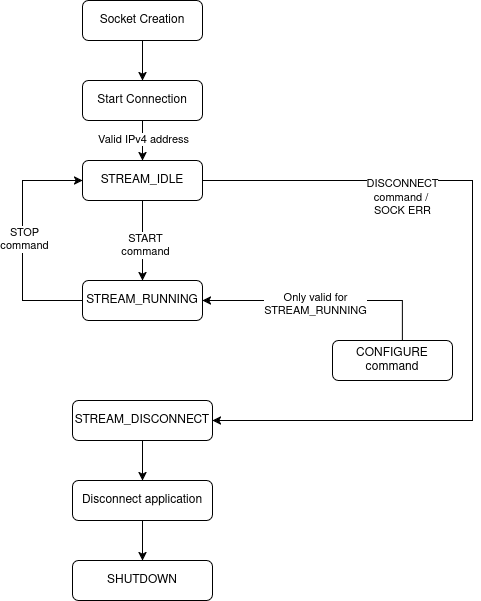
\includegraphics[scale = 0.5]{media/haizangui3.png}
\caption{Socket Creation}
\label{fig-haizangui3}
\end{figure}

\textbf{STREAM\_IDLE STATE}\\
This state represents the state where the application layer has made a successful connection with the GUI but the data is not streaming and the configuration commands are not applied. As the name suggests this is the idle state where the system remains connected.\\

\textbf{STREAM\_RUNNING STATE}\\
This state represents where the application layer is actively streaming data to the GUI and is ready to receive configuration commands from the GUI. This state is activated when the server receives the “START” command from the client side. The main action involved in this state is draining the ring buffer using the function \texttt{ringBufferRemoveBatch}, and then sending the payload in batches, to ensure proper use of TCP frames in the Ethernet connection.\\

To ensure data integrity and proper framing over a stream-oriented TCP connection, the implementation uses a length-prefixing technique. The server first calculates the total payload size, converts it to network byte order using htonl(), and sends this 4-byte header. Only after the header is successfully sent does it transmit the actual sensor data payload. The use of while loop around the send() calls accounts for partial writes, ensuring that every byte of the batch is delivered. If a transmission error occurs, the state machine transitions to \texttt{STREAM\_DISCONNECT}, where it gracefully shutdown the socket and releases resources to prevent memory leaks or hanging connections.\\

\textbf{STREAM\_DISCONNECT STATE}\\
Stream disconnect state is the state when the application layer has received the shutdown command and should kill the process. This is different from the idle state because it only shuts down connection with the client. This state represents the entire MNG application is offline.

\begin{minted}[bgcolor = lightgray, tabsize = 4, breaklines]{c}
if (stream_state == STREAM_DISCONNECT)
{
  printf("Closing client connection...\n");
  shutdown(client_fd, SHUT_RDWR);
  close(client_fd);
  break;
}
\end{minted}



\subsection{CONFIGURATION COMMANDS}
The network thread features an integrated command parser that allows external clients to dynamically control the MNG’s behavior. Upon receiving the data via recv(), the server sanitizes the input by stripping newline characters and comparing the string against a predefined command set. This allows for real-time state transactions, such as switching between \texttt{STREAM\_IDLE, STREAM\_RUNNING, STREAM\_DISCONNECT.}\\

\textbf{CONNECT COMMAND}\\
The connect command is for the socket connection between the application layer and the GUI. This command sends the IPv4 address which is used to connect. Only valid IPv4 address is used and hence required validation has been added in the GUI. \\


\textbf{START COMMAND}\\
The purpose of this command is to transfer the application from \texttt{STREAM\_IDLE} to \texttt{STREAM\_RUNNING} state, this will make the network layer drain the ring buffer and start sending the data in batches to the client. The START command is only valid if the application layer is connected and is not already streaming data to the GUI. Therefore required validation has been added in the GUI. 
\begin{minted}[bgcolor = lightgray, tabsize = 4, breaklines]{c}
if (!strcmp(cmd_buffer, "START"))
 {
    stream_state = STREAM_RUNNING;
 }
\end{minted}
\smallskip


\textbf{CONFIGURE COMMAND}\\
A significant feature of this section is the CONFIGURE command, which allows for live updates to individual sensor sampling rates. By parsing the command string with \texttt{sscanf()}, the server identifies the specific sensor and desired frequency in Hz. To maintain thread safety, the implementation utilizes POSIX mutexes (\texttt{pthread\_mutex\_lock}), ensuring that updating the \texttt{rate\_hz} and \texttt{period\_us} values does not create race conditions with the data acquisition thread. This architecture provides a clear separation of concerts: while the acquisition thread remains focused on high-speed sampling, the network thread provides a safe, low-latency interface for remote management and system shutdown. CONFIGURE command is only valid during STREAM\_RUNNING state and hence the required validation has been added to the GUI. 

\begin{minted}[bgcolor = lightgray, tabsize = 4, breaklines]{c}
if (!strncmp(cmd_buffer, "CONFIGURE", 9))
   {
       char sensor[16];
       uint32_t rate;

       if (sscanf(cmd_buffer, "CONFIGURE %15s %u", sensor, &rate) == 2)
       {
           int sid = sensor_from_string(sensor);
           if (sid >= 0 && rate > 0)
           {
               pthread_mutex_lock(&sensor_cfg[sid].lock);
               sensor_cfg[sid].rate_hz = rate;
               sensor_cfg[sid].period_us = 1000000ULL / rate;
               sensor_cfg[sid].next_deadline = getElapsedTime() + 
                                              sensor_cfg[sid].period_us;
               pthread_mutex_unlock(&sensor_cfg[sid].lock);
               printf("[SERVER] CONFIGURE applied\n");
           }
       }
   }
\end{minted}
\smallskip

\textbf{STOP COMMAND}\\
The stop command is used to send instructions to the application layer to stop streaming data to the GUI, while maintaining the connection. STOP command is only valid when the application layer was already streaming, hence such a validation is applied in the GUI. 

\begin{minted}[bgcolor = lightgray, tabsize = 4, breaklines]{c}
if (!strcmp(cmd_buffer, "STOP"))
{
  stream_state = STREAM_IDLE;
}
\end{minted}
\smallskip

\textbf{DISCONNECT COMMAND}\\
The disconnect command is used to disconnect the socket from the GUI. This is different from the IDLE state as the application and GUI are no longer connected. This command is only valid if the application layer and GUI are already connected via a valid IPv4 address and cannot be disconnected if the application layer is already streaming. The user will have to stop the streaming using STOP command first and then use DISCONNECT to cut the connection, and hence required validation has been added in the GUI.
\begin{minted}[bgcolor = lightgray, tabsize = 4, breaklines]{c}
if (!strcmp(cmd_buffer, "DISCONNECT"))
{
  stream_state = STREAM_DISCONNECT;
}
\end{minted}
\smallskip

\textbf{SHUTDOWN COMMAND}\\
Shutdown command is used to shutdown the whole application by setting the global variable system\_running to 0. This will clear all resources allocated and put the system to rest. 
\begin{minted}[bgcolor = lightgray, tabsize = 4, breaklines]{c}
if (!strcmp(cmd_buffer, "SHUTDOWN"))
{
  printf("Shutting down...\n");
  system_running = 0;
  stream_state = STREAM_DISCONNECT;
}
\end{minted}
\smallskip

\clearpage
\subsection{CONCLUSION}
The \texttt{networkThread.c} implementation delivers a structured, robust, and production-oriented communication layer for the Measurement Network Gateway. By isolating TCP communication within a dedicated thread, the design prevents network latency or client-side delays from interfering with deterministic sensor acquisition. This separation is not just architectural cleanliness — it is essential for maintaining real-time performance and system stability.

The use of a well-defined state machine \texttt{(STREAM\_IDLE, STREAM\_RUNNING, STREAM\_DISCONNECT)} ensures predictable behavior across the entire lifecycle of the connection. Explicit state transitions eliminate ambiguity, reduce unintended side effects, and simplify debugging. The implementation of length-prefixed TCP framing, combined with guarded \texttt{send()} loops, demonstrates careful handling of stream-oriented communication and partial writes a critical detail often overlooked in simpler designs.
Dynamic runtime configuration through structured command parsing enables flexibility without compromising thread safety. The use of POSIX mutexes to protect shared sensor parameters prevents race conditions, reinforcing the reliability of concurrent operations. Additionally, graceful shutdown handling ensures proper resource cleanup and prevents socket or memory leaks.
Overall, the module provides a reliable, low-latency, and extensible TCP server architecture capable of supporting real-time streaming and remote configuration. Its design reflects strong attention to concurrency control, communication integrity, and system resilience all essential characteristics of a well-engineed embedded networking solution.

\clearpage 
\null 
\vfill 
\begin{center}
\textbf{\large Alin Raj Rajagopalan Nair (41520)}
\end{center}
\vfill 
\fancyhead[L]{MNG Application (Alin Raj Rajagopalan Nair 41520)}
\clearpage

\chapter{MNG Application part II}
\section{MAX31865}
\subsection{Temperature Conversion}
Sensors that change resistance in response to temperature are known as
resistance temperature detectors (RTDs). Platinum RTDs, also known as
PT-RTDs, are the most widely used and precise wire material. RTDs can
also be made of copper, nickel, and other metals. Platinum RTDs provide
good accuracy and repeatability, decent linearity, and a broad
temperature range (to above +800NC). Although there are additional
numbers available, 100I and 1kI are the most often used nominal
resistance levels for PT-RTDs at 0NC. Alpha (α) is the average slope
between 0NC and +100NC. The contaminants and their concentrations in the
platinum determine this value. The two most commonly used alpha values,
which correspond to the SAMA and IEC 751 (PT100) standards, are 0.00385
and 0.00392 temperature Conversion.

Based on this the resistance vs temperature graph is almost linear , but
at some points the curvature exists as mentioned in the ~Callendar- Van
Dusen equation:

\begin{align*}
R(T) = R_0 \cdot (1 + aT + bT^2 +c \cdot (T - 100) T^3)
\end{align*}

where: 

$T$: Temperature (\unit{\degreeCelsius})\\
$R(T)$: resistance at T \\ 
$R_0$: resistance at $T = \SI{0}{\degreeCelsius}$\\ 
$\alpha$: 0.00385055 is specified in the IEC 751\\ 
The following are the Callender-Van Dusen coefficient values: 
$a = 3.90830 \times 10^{-3}$\\
$b = -5.77500 \times 10^{-7}$\\ 
$c = -4.18301 \times 10^{-12}$ for $-200 \unit{\degreeCelsius} \leq T \leq 0 \unit{\degreeCelsius}$, 0 for $0 \unit{\degreeCelsius} \leq T + 850 \unit{\degreeCelsius}$ 
Figure illustrates that the resistance of a PT100 RTD increases with
temperature in a slightly nonlinear manner, following the standardized
platinum resistance--temperature relationship. For practical purposes
within the 0 \unit{\degreeCelsius} to 100 \unit{\degreeCelsius} range, this characteristic can be approximated
by a straight line with a slope of approximately 0.385 \unit{\ohm}/\unit{\degreeCelsius}, which
simplifies calculations while introducing only minimal deviation from
the actual curve.

\begin{figure}[H]
\centering 
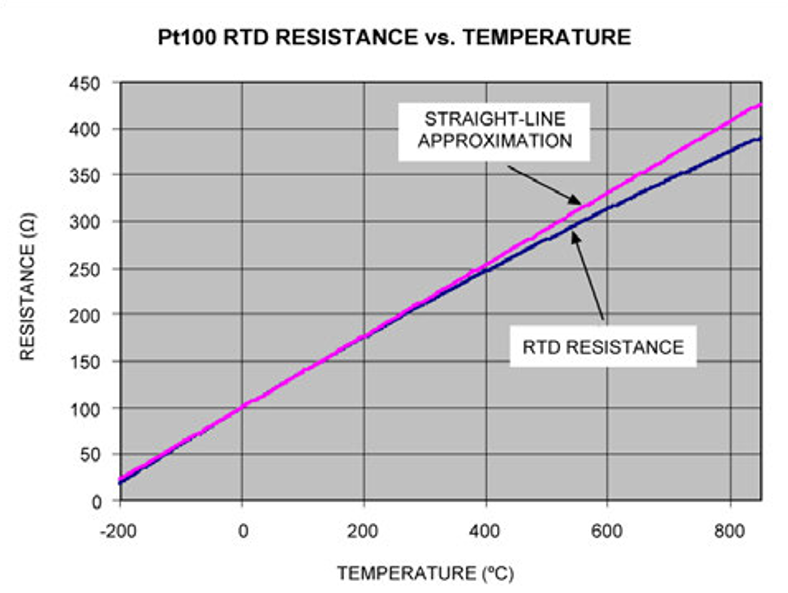
\includegraphics[width = 0.6\textwidth]{media/alin1.png}
\caption{PT100 RTD Resistance vs Temperature}
\label{fig-alin1}
\end{figure}

\subsection{Typical Application Circuits}
There are 3 ways in which we can typically measure the resistance and
they are listed as follows

\begin{enumerate}
\item 2-Wire Measurement: In a 2-wire configuration, the same pair of conductors is used both to supply the excitation current and to sense the voltage across the RTD, which means the resistance of the lead wires is directly added to the sensor resistance. 
For a PT100, whose sensitivity is approximately 0.385 \unit{\ohm / \degreeCelsius}, an additional series 
resistance of 0.4 \unit{\ohm} corresponds to a temperature error of about 1 \unit{\degreeCelsius} (0.4 \unit{\ohm} ÷ 0.385 \unit{\ohm / \degreeCelsius} $\approx$ 1 \unit{\degreeCelsius}). While this error may be negligible when the RTD is mounted very close 
to the MAX31865 and the lead length is short, the resistance of longer cables increases proportionally with length and conductor size, causing a systematic positive temperature to offset. Consequently, in installations with extended wiring, the accumulated lead resistance can introduce significant measurement inaccuracies, making 3-wire or 4-wire configurations preferable for improved compensation and precision.

\begin{figure}[H]
 \centering 
 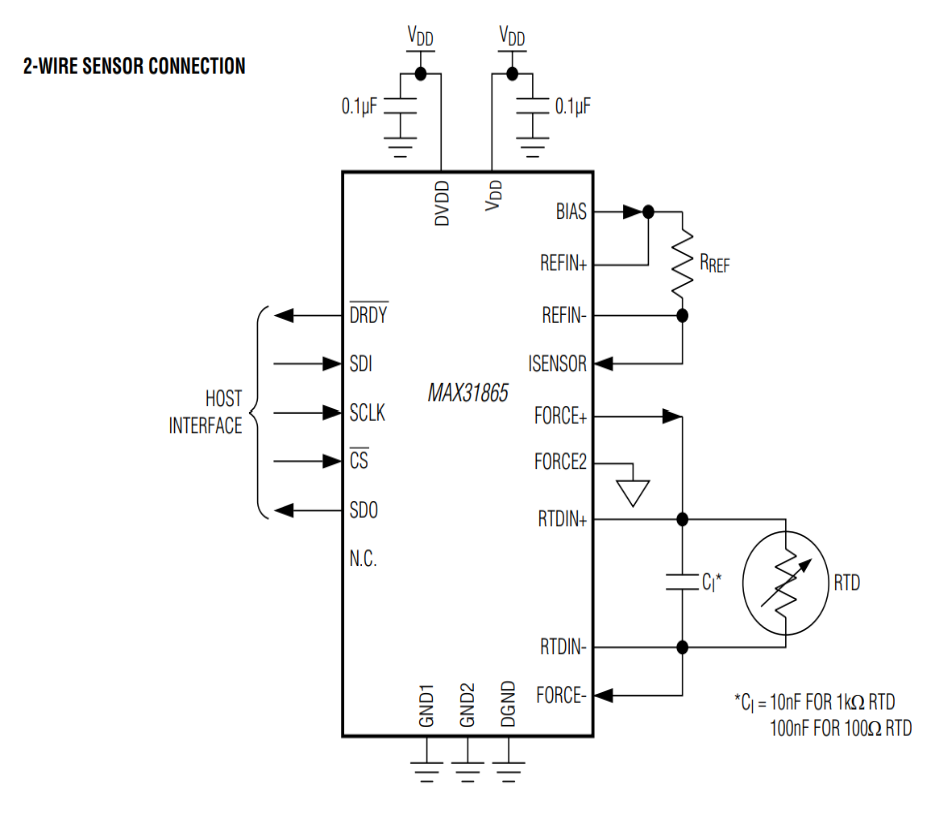
\includegraphics[scale = 1]{media/alin2b.png}
 \caption{Wire Sensor Connection circuit}
 \label{fig-alin2}
 \end{figure} 
 
 
 
\item 3-Wire Measurement: In a 3-wire configuration, two conductors are connected to one side of the RTD element and a third conductor is connected to the opposite side, allowing partial compensation of lead resistance while using fewer wires than a full 4-wire (Kelvin) setup. The MAX31865 applies a precise excitation current through the RTD and measures two voltages: the voltage across the RTD terminals (RTDIN+ to RTDIN−) and the voltage drop across the current-carrying return lead (via the FORCE2 sampling input). By subtracting the measured lead voltage from the total sensed voltage, the device effectively removes the contribution of one lead resistance from the calculation.

      This compensation method assumes that the two current-carrying leads have approximately equal resistance; when they are well matched in length and cross-section, their voltage drops are nearly identical and cancel each other, significantly reducing measurement error. Although a small residual error may remain if the lead resistances are unequal or subject to temperature gradients, the 3-wire approach provides a practical balance between wiring complexity and measurement accuracy, making it the most widely used configuration in industrial PT100 applications.

\begin{figure}[H]
\centering 
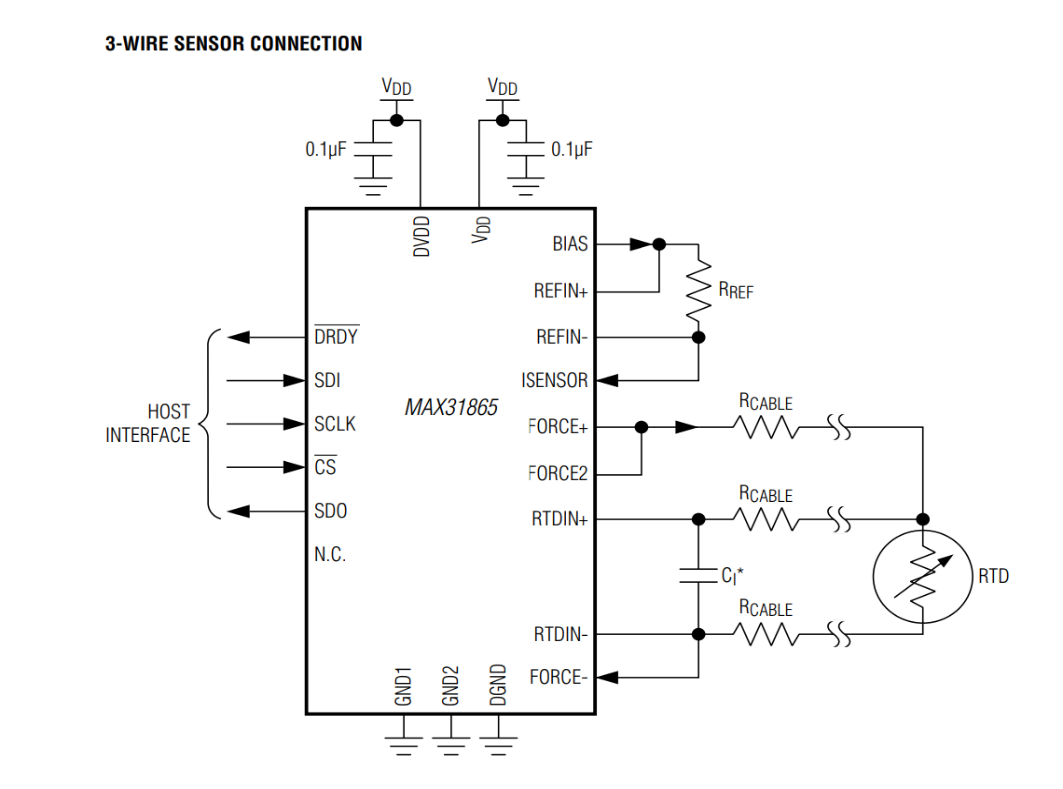
\includegraphics[scale = 1]{media/alin3.png}
\caption{3-Wire Sensor Connection}
\label{fig-alin3}
\end{figure}

\item 	4-Wire Measurement: The 4-wire connection eliminates errors due to cable resistance by using two conductors to supply the excitation (force) current and two separate conductors to sense the voltage directly across the RTD element. Because the sense inputs draw negligible current, virtually no voltage drop occurs along the sense leads, meaning the measured voltage reflects only the true RTD resistance and not the resistance of the connecting wires. As a result, the calculated resistance
 ( $R=V/I$ ) is independent of cable length and lead resistance, providing the highest possible measurement accuracy, particularly in applications with long cable runs or where precise temperature determination is required.
 
 \begin{figure}[H]
 \centering 
 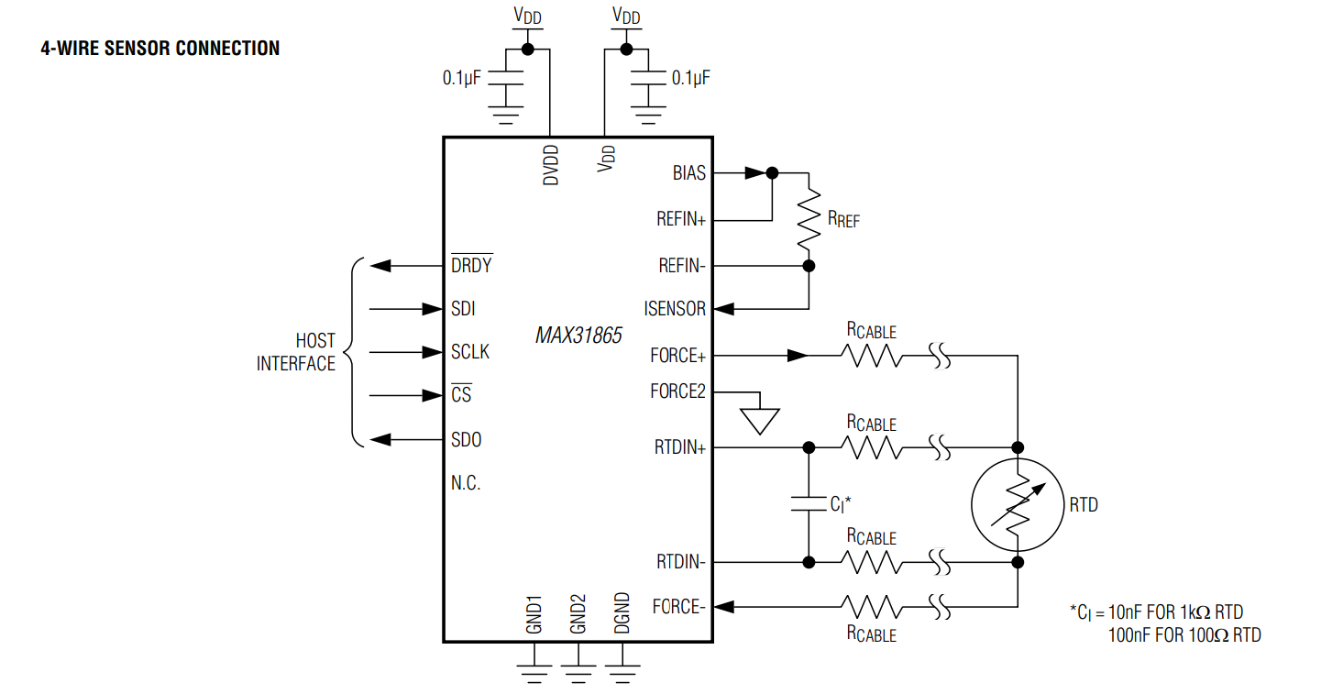
\includegraphics[scale = 1]{media/alin4.png}
 \caption{4-Wire Sensor Connection circuit}
 \label{fig-alin4}
 \end{figure}
\end{enumerate}

\section{Internal Registers}
\subsection{Introduction}
The MAX31865 is a precision RTD-to-digital converter designed to interface platinum RTDs such as PT100 and PT1000 with a microcontroller via an SPI interface. It integrates a precision bias current source, a 15-bit sigma-delta ADC, fault detection circuitry, and digital filtering. All device configuration, measurement data, and diagnostic information are accessed through a small set of internal registers. These registers allow the user to control operating modes, read conversion results, define fault thresholds, and monitor system integrity. 
The registers are accessed using the 0Xh addresses for reads and the 8Xh addresses for writes. Data is read from or written to the registers MSB first.
\begin{figure}[H]
\centering 
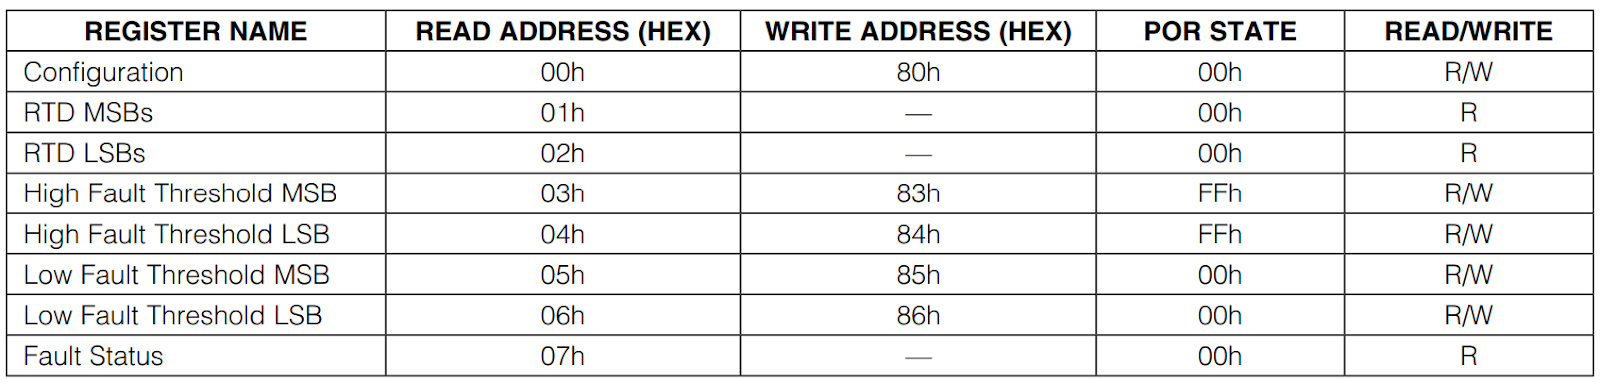
\includegraphics[width = \textwidth]{media/alin2.png}
\caption{Internal registers of MAX31865}
\label{fig-alin2bc}
\end{figure}

\subsection{Configuration Registers (00h)}
The Configuration Register (address 00h) is an 8-bit control register that determines the complete operating behaviour of the MAX31865. It governs excitation control, ADC conversion timing, wiring compensation, fault detection routines, and digital noise filtering. Since the MAX31865 performs ratio-metric resistance measurement using a precision reference resistor, correct initialization of this register is essential for stable and accurate RTD measurements.

\textbf{Operational Control and Measurement Modes}
One of the primary functions of this register is to control how conversions are executed. The device can operate in:

\begin{itemize}
\item Continuous (automatic) conversion mode, where the sigma-delta ADC continuously updates the RTD data registers at fixed intervals. This mode is suitable for real-time temperature monitoring systems.
\item Normally-off mode, where the ADC remains idle until a 1-shot conversion is triggered. This approach reduces power consumption and minimizes RTD self-heating, which is particularly important in precision or battery-powered applications.
\end{itemize}
The 1-shot control bit initiates a single conversion cycle and automatically clears once the conversion is complete.

\begin{figure}[H]
\centering 
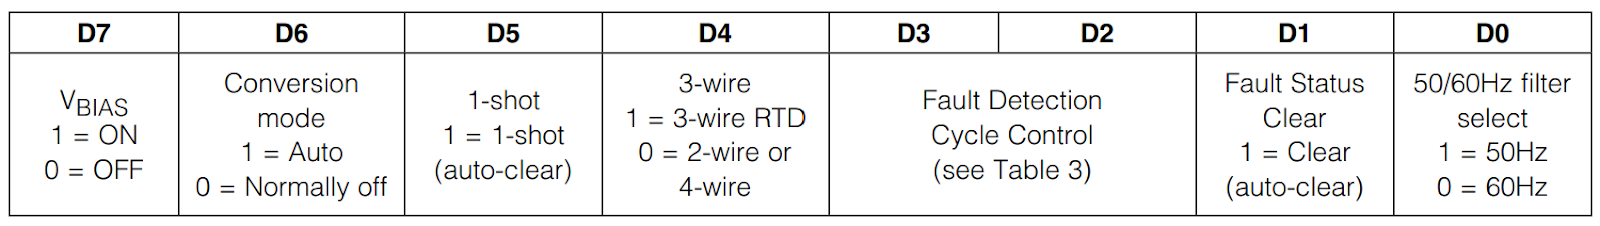
\includegraphics[width = \textwidth]{media/alin5.png}
\caption{Configuration register of MAX31865}
\label{fig-}
\end{figure}

\subsubsection{BIAS (D7)}
The configuration register controls the activation of the internal bias voltage (VBIAS), which provides the excitation current required for RTD measurement. When VBIAS is enabled, a controlled current flows through both the RTD and the precision reference resistor, allowing the ADC to measure the ratio of their voltages and accurately determine the RTD resistance. However, if no conversion is being performed, VBIAS can be disabled to stop the excitation current, thereby reducing power dissipation, minimizing sensor self-heating effects, and limiting long-term thermal drift.

In single (1-shot) conversion mode, it is good practice to set the VBIAS bit to ‘1’ shortly before initiating a conversion, allow a brief stabilization time, and then trigger the measurement. After the conversion is complete, VBIAS may be cleared again to conserve energy and maintain measurement accuracy. In contrast, when automatic (continuous) conversion mode is selected, the bias voltage remains enabled continuously to support uninterrupted ADC operation and real-time temperature monitoring.

\subsubsection{Conversion Mode (D6)}
The Conversion Mode bit in the configuration register determines whether the MAX31865 operates in continuous measurement mode or in normally-off (manual) mode. When this bit is set to ‘1’, the device enters automatic conversion mode, in which the internal sigma-delta ADC performs conversions continuously at a rate synchronized with the selected 50 Hz or 60 Hz digital filter. In this mode, new RTD data is updated automatically at regular intervals, making it suitable for real-time temperature monitoring applications where continuous measurement is required.

When the bit is cleared to ‘0’, the device exits automatic mode and enters Normally Off mode, in which no conversions are performed unless explicitly commanded. This mode is commonly used in low-power or precision systems to reduce energy consumption and minimize RTD self-heating. While in Normally Off mode, a single measurement can be initiated by setting the 1-shot bit, which triggers one complete conversion cycle. After the conversion is finished, the ADC returns to the idle state until another 1-shot command is issued.

Thus, the Conversion Mode bit allows the user to select between continuous real-time measurement and controlled, on-demand conversion depending on system requirements for power efficiency and measurement frequency.

\subsubsection{Shot-bit (D5)}
The 1-Shot bit (D5) is used to initiate a single resistance conversion when the device is operating in Normally Off mode (i.e., when the Conversion Mode bit is set to ‘0’). Writing a logic ‘1’ to this bit commands the MAX31865 to perform one complete ADC conversion cycle. The actual conversion process begins when the SPI transaction ends and the CS (Chip Select) line transitions high after the bit has been written.

Once triggered, the device performs a full resistance measurement using the selected digital filter setting. The conversion time depends on the chosen mains rejection filter:
\begin{itemize}
\item Approximately 52 ms when the 60 Hz filter is selected
\item Approximately 62.5 ms when the 50 Hz filter is selected
\end{itemize}

The longer duration in 50 Hz mode is due to the digital filtering process, which integrates over one full mains cycle to effectively suppress line-frequency noise.

The 1-Shot bit is self-clearing, meaning it automatically returns to ‘0’ once the conversion has started. This ensures that only a single measurement cycle is executed per command and prevents unintended repeated conversions. After completion, the ADC result is stored in the RTD data registers, and the device returns to the idle state until another 1-Shot command is issued.
This feature is particularly useful in low-power applications, where measurements are taken periodically rather than continuously, helping to minimize power consumption and RTD self-heating effects.

\subsubsection{bit (D4)}
The 3-Wire bit (D4) configures the MAX31865 for use with a 3-wire RTD connection. When this bit is set to ‘1’, the device activates its internal lead-resistance compensation circuitry. In this configuration, the MAX31865 measures the voltage between FORCE+ and RTDIN+ and subtracts it from the total measured voltage (RTDIN+ − RTDIN−). This subtraction compensates for the voltage drop (I·R drop) that occurs along the shared return lead, which carries both excitation current and sense current in a 3-wire arrangement.

The compensation method assumes that the two current-carrying leads have approximately equal resistance. When the lead resistances are well matched, the IR errors introduced by cable resistance are effectively cancelled, significantly improving measurement accuracy compared to a 2-wire configuration. However, if the lead resistances differ due to unequal cable lengths or temperature gradients, a small residual error may remain.

When using either a 2-wire or 4-wire RTD configuration, this bit must be written as ‘0’, disabling the internal 3-wire compensation circuitry and ensuring correct measurement operation for those wiring modes. Proper setting of the 3-Wire bit is essential to avoid incorrect resistance calculations and measurement inaccuracies.


\subsubsection{Fault Detection Cycle Bits (D3:D2)}
The Fault Detection Cycle bits (D3:D2) control the execution of the master-initiated diagnostic routine within the MAX31865. This routine is used to detect wiring faults and abnormal operating conditions such as open-circuit RTDs, short circuits, reference resistor faults, and overvoltage or undervoltage conditions. The fault detection mechanism applies specific internal test conditions to the RTD inputs and evaluates the resulting signals to determine whether a fault exists.

The fault detection cycle can operate in automatic timing mode or manual timing mode. In automatic mode, the device internally manages the timing sequence of the diagnostic procedure. The user only initiates the cycle, and the MAX31865 completes the test according to its predefined internal timing intervals. This mode is suitable for standard applications where no significant external filtering affects signal response.

In contrast, manual mode timing allows the system controller (microcontroller) to manage the timing steps of the fault detection process. This is particularly important when the external RTD interface circuitry includes additional input filtering components with a time constant greater than approximately 100 µs. Large time constants slow the settling of voltages during diagnostic testing, and automatic timing may not allow sufficient time for signals to stabilize. In such cases, manual control ensures accurate fault detection by providing adequate settling time between test phases.

Therefore, the selection between automatic and manual fault detection timing depends on the external analog filtering characteristics and overall system design requirements.

\subsubsection{Fault Status Clear Bit (D1)}
The Fault Status Clear bit (D1) is used to reset all latched fault indicators stored in the Fault Status Register. To properly clear the fault flags, a logic ‘1’ must be written to D1 while simultaneously ensuring that bits D5 (1-Shot) and D3:D2 (Fault Detection Cycle) are written as ‘0’. When this condition is met, all fault status bits D[7:2] in the Fault Status Register are cleared and returned to ‘0’.

It is important to note that clearing the fault register does not remove the actual fault condition from the system. If the underlying issue—such as an overvoltage or undervoltage condition—still exists, the corresponding fault bit (specifically bit D2 in the Fault Status Register) may be set again immediately after the reset operation. Consequently, the fault indicator bit in the RTD LSB register (D0) may also be reasserted if the fault persists.

The Fault Status Clear bit is self-clearing, meaning it automatically returns to ‘0’ after the clearing operation is completed. This ensures that the reset action occurs only once per command and prevents unintended repeated clearing of diagnostic flags.

\subsubsection{50/60 Hz Filter Select Bit (D0)}
The 50/60 Hz bit (D0) selects the notch frequency of the internal digital noise rejection filter in the MAX31865. This filter is designed to suppress interference from mains power frequencies that can couple into the RTD wiring and affect measurement accuracy. Since industrial and laboratory environments often contain electromagnetic noise at the local power-line frequency, proper selection of this bit significantly improves measurement stability.

When D0 = 0, the device configures its digital filter to reject 60 Hz and its harmonic components. This setting is typically used in regions where the mains supply frequency is 60 Hz. Conversely, when D0 = 1, the filter is configured to reject 50 Hz and its harmonics, which is appropriate for regions operating on a 50 Hz power grid.

The filter works by synchronizing the ADC integration time with the selected mains frequency, effectively averaging out periodic noise components. As a result, selecting the correct notch frequency reduces ripple, improves signal stability, and enhances overall temperature measurement accuracy in electrically noisy environments.

\subsubsection{RTD Resistance Registers (01h–02h)}
The RTD Resistance Registers (addresses 01h and 02h) store the digital conversion result of the measured RTD resistance. These consist of two 8-bit registers: the RTD MSB register (01h) and the RTD LSB register (02h). Together, they form a 16-bit word in which the upper 15 bits represent the measured resistance value, while the least significant bit (D0 of the LSB register) serves as a fault indicator.

The measurement result is expressed as a 15-bit ratio of the RTD resistance to the external reference resistor resistance. Internally, the MAX31865 performs a ratio metric measurement using its sigma-delta ADC, comparing the voltage drop across the RTD to the voltage across the precision reference resistor. The resulting digital code corresponds to:\\

ADC code = $R_{RTD} / R_{REF} \cdot 2^15$ \\ 
To calculate the actual RTD resistance, the following relationship is used:\\

$R_{RTD} = (ADC\ code / 32768) \cdot R_{REF}$\\

where 32768 represents the full-scale value of the 15-bit ADC.

Bit D0 of the RTD LSB register is reserved as a Fault flag. If this bit is set to ‘1’, it indicates that a fault condition has been detected, and the system should check the Fault Status Register (07h) to determine the specific cause.

These registers provide the primary measurement data required for temperature calculation and are read by the microcontroller after each completed conversion. 

\begin{figure}[H]
\centering 
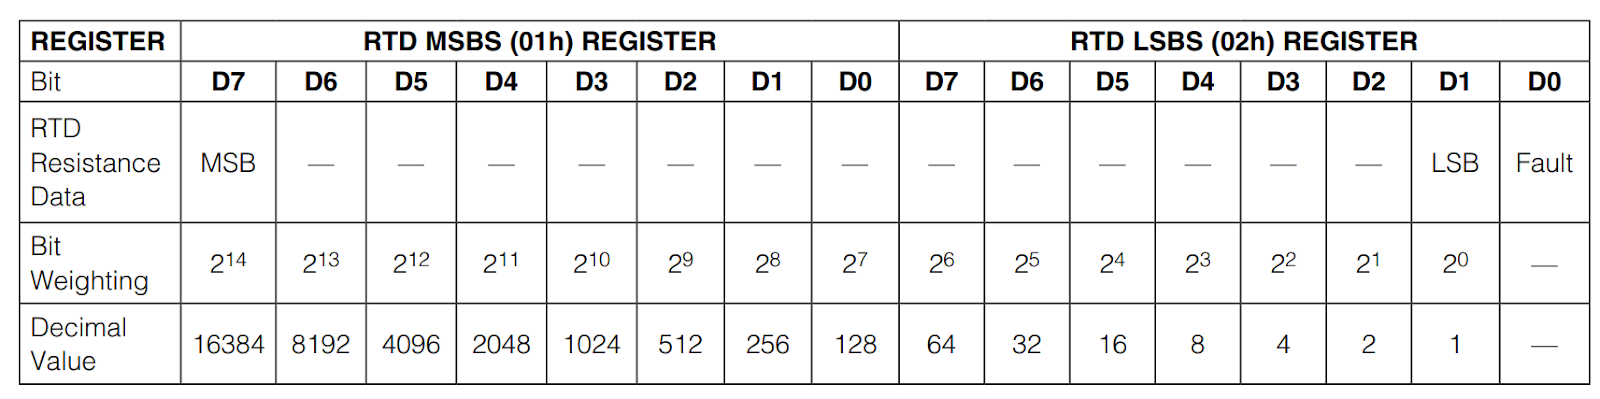
\includegraphics[width = \textwidth]{media/alin6.png}
\caption{RTD Resistance register layout}
\label{fig-alin6}
\end{figure}

\section{Types of Operation}
\subsection{Writing to MAX31865 registers (writeMAXSpiInterface())}
To write to any register in the MAX31865, the function writeMAXSpiInterface() is used. This function constructs a 16-bit SPI data frame where the Most Significant Byte (MSB 8 bits, bit 15 to 8) contains the register address with the write bit set, and the Least Significant Byte (LSB 8 bits, bit 7 to 0) contains the data value to be written. Every MAX31865 register has one read address and one write address [if the register is read-only, then writing to it does not affect its contents].\\

write address = read address | 0x80\\

example: writing 0xA1 in configuration register
read address of configuration register is 0x00 so its write address becomes 0x80.\\

MSB 8 bits (15 to 8) becomes 0x80 and LSB 8 bits (7 to 0) becomes 0xA1. so the whole data frame becomes 0x80A1. Writing this data frame to the kernel module register via \\ 

\textbf{\texttt{write(fd, \&tf\_obj\_snd, MEASOBJ\_SIZE);}}\\
will initiate the SPI communication.
The function then polls the status register by checking bit 0. When the status bit becomes 1, the SPI transaction is complete.
For writing to MAX31865, the function 
\begin{figure}[H]
\centering 
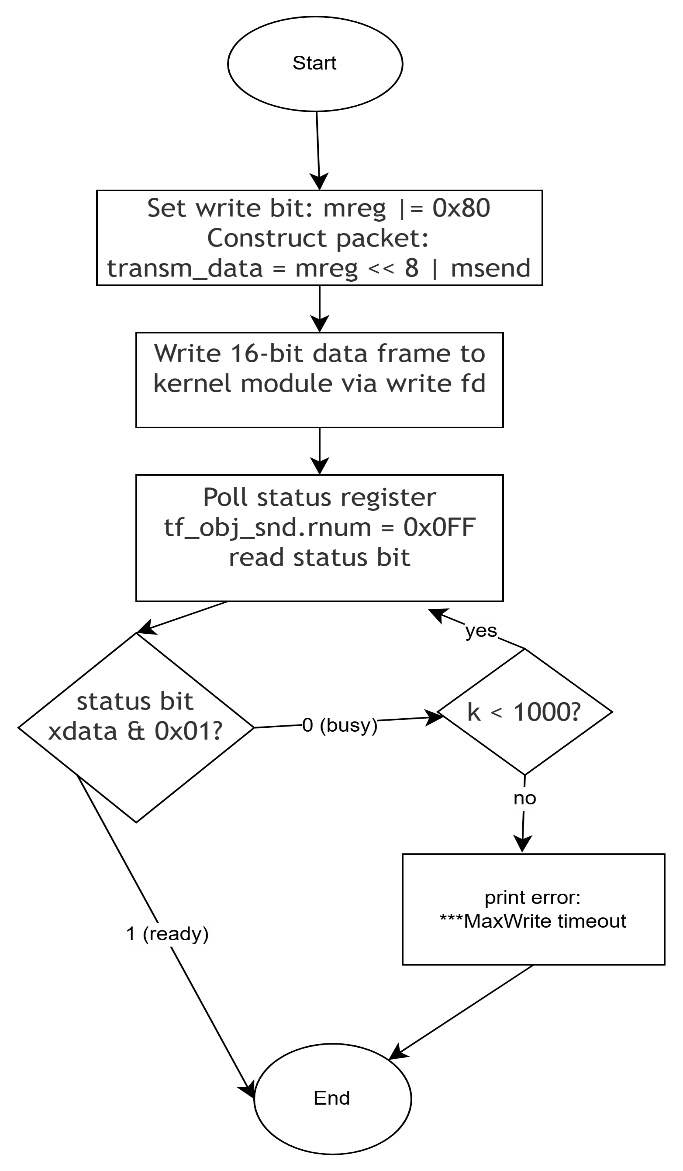
\includegraphics[scale = 1]{media/alin7.png}
\caption{write algorithm}
\label{fig-}
\end{figure}

\textbf{\texttt{writeMAXSpiInterface(int fd, unsigned int mreg, unsigned int msend); }}\\
is used, where "fd" is the file descriptor for /dev/meascdd, "mreg" is the register address in which data is to be written, and "msend" is the 8-bit value to be written.
for example: writing to configuration register using "writeMAXSpiInterface" function.\\

\textbf{\texttt{writeMAXSpiInterface(fd,MAX31865\_REG\_CONFIG,0xa1);}}\\
where MAX31865\_REG\_CONFIG = 0x00 (configuration register address) and 0xa1 is the configuration value (VBIAS=1, 1SHOT=1, 50Hz filter enabled).
for example: writing to high fault threshold MSB register

\textbf{\texttt{writeMAXSpiInterface(fd, 0x03, 0xff);}}
where 0x03 is the high fault threshold MSB register address and 0xff is the threshold value.

\subsection{Reading from MAX31865}
To read from registers of MAX31865, Same data frame is used.
MSB 8 bits are used for defining the register address to be read.
LSB 8 bits does not matter.
for example to read RTD MSB register (read address 0x01): MSB 8 bit becomes 0x01. So the whole data frame is 0x01XX (where XX typically is 0x00, making the frame 0x0100).
Writing the data frame to kernel module via \textbf{\texttt{write(fd, \&tf\_obj\_snd, MEASOBJ\_SIZE)}} starts the communication.

\begin{figure}[H]
\centering 
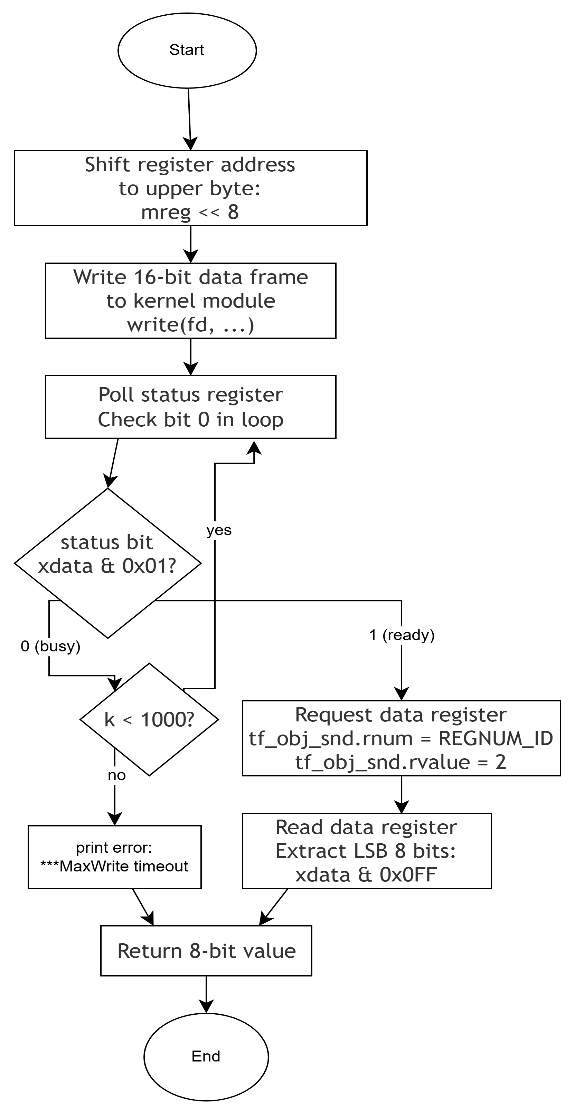
\includegraphics[scale = 1.2]{media/alin9.png}
\label{fig-alin8}
\end{figure}

when the status bit becomes 1, it indicates the read operation was successful and the result of read will be stored in the kernel module's data register.
But only LSB 8 bits of the returned value will be the data as all the MAX31865 registers are 8 bits. So the result must be masked with 0x0FF to extract the valid data: xdata \&= 0x0FF.

reading from MAX31865 with, \textbf{\texttt{readMAXSpiInterface(int fd, unsigned int mreg)}}
, where "fd" is the file descriptor and "mreg" is the register to be read.\\

Example: Reading RTD MSB register (read address: 0x01)\\
 
\texttt{msb = readMAXSpiInterface(fd, MAX31865\_REG\_RTD\_MSB);}\\
 
where \texttt{MAX31865\_REG\_RTD\_MSB = 0x01}\\

Example: Reading RTD LSB register (read address: 0x02)\\

\texttt{lsb = readMAXSpiInterface(fd, MAX31865\_REG\_RTD\_LSB);}\\

where \texttt{MAX31865\_REG\_RTD\_LSB = 0x02}. This register contains RTD bits [6:0] plus fault bit at bit 0.


\subsection{Taking Temperature Reading from MAX31865}
\begin{enumerate}
\item setting 7th, 5th, 0th bits of configuration register to 1. 
	\begin{itemize}
		\item 7th bit is for turning on MAX31865 (VBIAS), continuously keeping the sensor on will consume power so it is enabled only during measurement.
\item 5th bit is for one shot conversion - triggers a single temperature measurement.
\item 0th bit is for setting filter frequency to 50 Hz to reject power line noise.
Note: for detailed bit description see the datasheet of MAX31865 configuration register section
	\end{itemize}
	
\item Wait for 1 millisecond \texttt{(usleep(1000))} to allow the MAX31865's internal ADC to complete the resistance-to-digital conversion.

\item Read RTD MSB register (read address: 0x01) using readMAXSpiInterface(). This contains bits [14:7] of the 15-bit RTD value.
\item Then RTD LSB register (read address: 0x02) is read. This contains bits [6:0] of RTD value plus fault bit at bit 0.

\item Then MSB 8 bits and LSB 8 bits are merged using: \texttt{rtd = (msb << 8) | lsb}

\item Check if bit 0 (fault bit) is set using rtd \& 0x01. If fault is detected, read fault register (0x07) and return error code -1.

\item If no fault, right shift by 1 as 0th bit of RTD LSB reg is \texttt{fault-bit: rtd >>= 1}

\item Remaining 15-bit "result" is the RTD resistance code which can be used to calculate temperature from equation given in datasheet of MAX31856.
T(\unit{\degreeCelsius}) $\approx$ (result)/32 – 256, this equation is approximated.

\item RTD value is stored in \texttt{sample.sensor\_value} along with timestamp.

\item Sample is added to ring buffer using ringBufferAddSample(rb, \&sample) for transmission to network clients.
\end{enumerate}
\begin{figure}[H]
\centering 
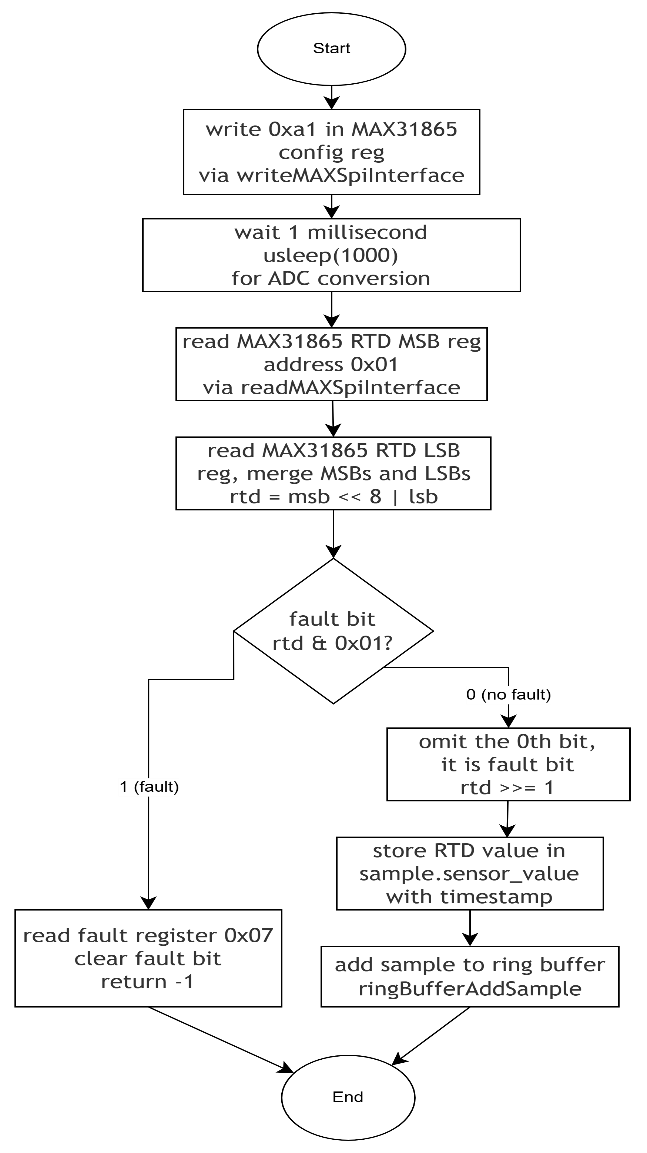
\includegraphics[scale = 1.2]{media/alin8.png}
\label{fig-alin8}
\end{figure}

\section{Shutdown Process}
The system shutdown process ensures graceful termination of all sensor operations and proper power-down of the MAX31865 temperature sensor. The shutdown sequence is coordinated through a global flag (system\_running) and involves multiple cleanup steps to ensure hardware safety and resource management.

\textbf{Shutdown Control Mechanism: }
\begin{minted}[bgcolor = lightgray, tabsize = 4, breaklines]{c}
volatile int system_running = 1;
\end{minted}

States:\\
utsystem\_running = 1 → System active, continue operation\\
system\_running = 0 → Shutdown requested, begin cleanup\\
Type: volatile ensures the variable is read from memory on every access, allowing immediate response to shutdown requests from any thread or signal handler.

\subsection{Shutdown Triggers}
The shutdown sequence can be initiated by three mechanisms:

\subsubsection{Network Command (Primary Method)}
\begin{minted}[bgcolor = lightgray, tabsize = 4, breaklines]{c}
if (strcmp(command, "SHUTDOWN") == 0) { 
printf("[NET] Shutdown command received\n"); 
system_running = 0; }
\end{minted}

\textbf{Process:}
\begin{itemize}
\item TCP client sends "SHUTDOWN\textbackslash n" command
\item Network thread sets global flag to 0
\item Sensor thread detects change and begins shutdown
\end{itemize}

\subsubsection{Signal Handler (Ctrl+C or Kill)}
\begin{minted}[bgcolor = lightgray, tabsize = 4, breaklines]{c}
void signal_handler(int signum) {
    printf("\n[MAIN] Shutting down...\n");
    system_running = 0; }
\end{minted}

\subsubsection{Error Condition}
Automatic shutdown on critical failures:

\begin{minted}[bgcolor = lightgray, tabsize = 4, breaklines]{c}
if (critical_error) {
    system_running = 0; }
\end{minted}

\textbf{Key Takeaways}
\begin{enumerate}
\item Flag-Based Control: Single global flag (system\_running) controls shutdown
\item Graceful Exit: Current operations complete before shutdown
\item Power-Down Critical: VBIAS disabled via 0x01 configuration
\item Resource Cleanup: Device file closed, thread exits cleanly
\item Fast Shutdown: Typically 1-2 ms from trigger to complete
\item Safe Restart: Clean state allows quick re-initialization
\item Power Savings: 72\% reduction in system power consumption
\end{enumerate}

\section{Reading and Writing to the Slave Registers}
\texttt{MeasObj\_struct} is used to read and write to hardware registers.
Data is written to hardware registers using the global variable \texttt{tf\_obj\_snd} of type \texttt{measObj\_struct}. Data is read from hardware registers using the global variable tf\_obj\_rcv of type measObj\_struct. The device file \texttt{(/dev/meascdd)} is used for all reading and writing operations involving hardware registers.

\subsection{Writing into the slave registers}
\begin{figure}[H]
\centering 
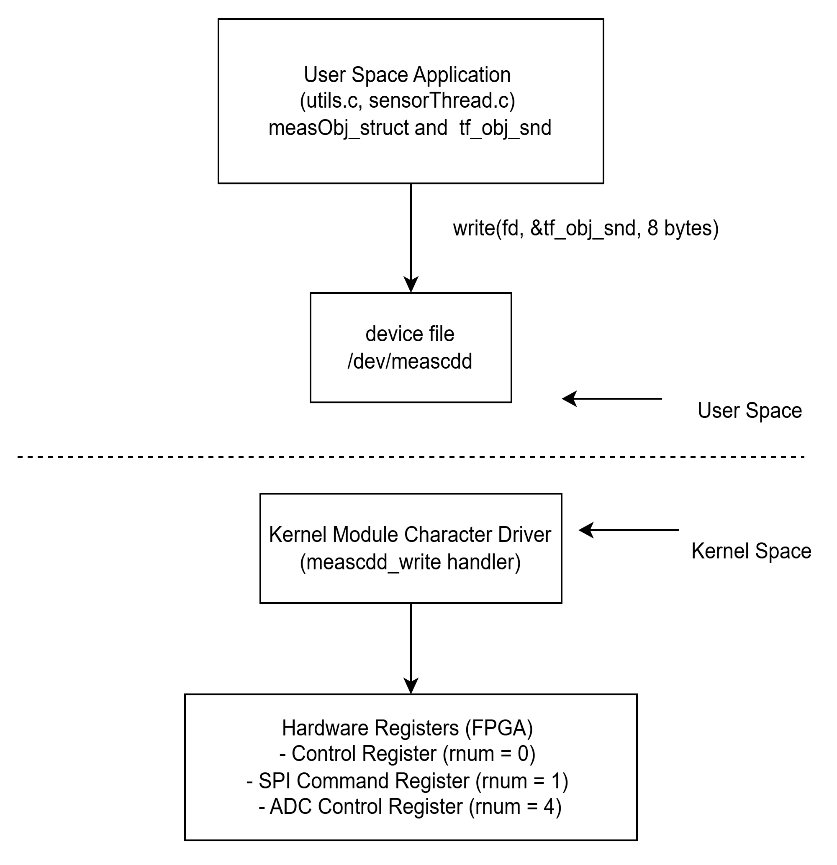
\includegraphics[scale = 1.2]{media/alin10.png}
\caption{Writing into slave registers}
\label{fig-alin10}
\end{figure}

For writing to Hardware registers 
\texttt{tf\_obj\_snd.rnum = reg;
tf\_obj\_snd.rvalue = value;}

where:

\begin{itemize}
\item "reg" is the register number (rnum selector)
\item "value" is the value to be written to the hardware register
\end{itemize}
Writing this structure to the device file via write() system call will write the "value" to the hardware registers.

\textbf{Key Points}
Kernel Module Interface: Unlike direct register access, our code uses a kernel module \texttt{(/dev/meascdd)} for hardware access. 

\begin{itemize}
\item Two-Level Addressing: 
\item First level: rnum selects the hardware register type (control, SPI, ADC)
\item Second level: For SPI operations, the 16-bit rvalue contains [address][data]
\item Status Polling: Every write operation includes status checking to ensure completion. 
\item Safety: The kernel module validates all operations before accessing hardware. 
\item Portability: Same application code works on any Linux system with the appropriate kernel module.
\end{itemize}

\begin{figure}[H]
\centering 
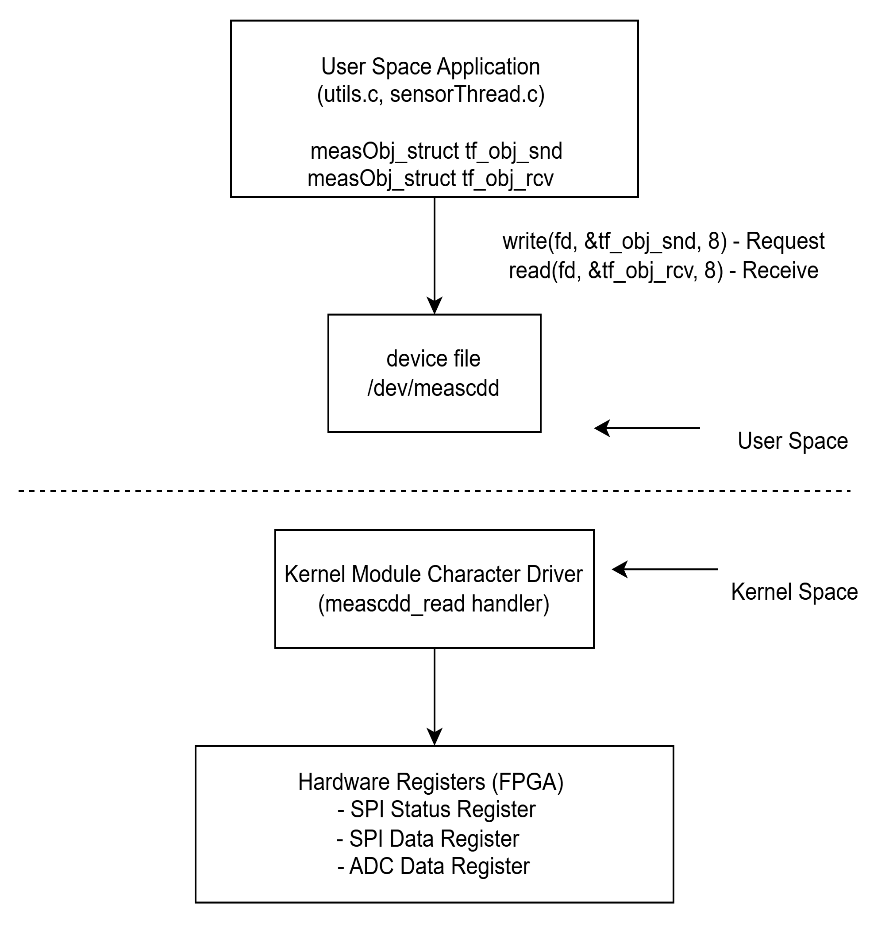
\includegraphics[scale = 1.2]{media/alin11.png}
\caption{Reading From Slave Registers}
\label{fig-alin11}
\end{figure}

For reading from hardware registers, a two-step process is used:
Step1: Send Read Command
\begin{minted}[bgcolor = lightgray, tabsize = 4, breaklines]{c}
tf_obj_snd.rnum = 1;        // SPI command register
tf_obj_snd.rvalue = mreg;   // Register address to read
write (fd, &tf_obj_snd, MEASOBJ_SIZE); 
\end{minted}

Step 2: Poll Status and Retrieve Data:
\begin{minted}[bgcolor = lightgray, tabsize = 4, breaklines]{c}
// Poll for completion

do {
    tf_obj_snd.rnum = REGNUM_ID;                          // Status register
    tf_obj_snd.rvalue = 1;                                             // Status query
    write(fd, &tf_obj_snd, MEASOBJ_SIZE);
    read(fd, &tf_obj_rcv, MEASOBJ_SIZE);
} while ((tf_obj_rcv.rvalue & 0x01) == 0);

// Retrieve data

tf_obj_snd.rnum = REGNUM_ID;
tf_obj_snd.rvalue = 2;                                                 // Data selector
write(fd, &tf_obj_snd, MEASOBJ_SIZE);
read(fd, &tf_obj_rcv, MEASOBJ_SIZE);

result = tf_obj_rcv.rvalue & 0xFF;                              // Extract 8-bit result
\end{minted}

\begin{itemize}
\item "REGNUM\_ID" (0x0FF) is the status/data register selector
\item "rvalue = 1" requests status information
\item "rvalue = 2" requests data result
\item The final result is masked to extract the 8-bit value
\end{itemize}

Reading from the device file via read() system call retrieves data from hardware registers into the tf\_obj\_rcv structure.

\textbf{Key Points}
\begin{enumerate}
\item Two-Phase Read: Read operations require sending a read command, then retrieving the result.
\item Status Polling: Every read includes status checking to wait for hardware completion.
\item Data Extraction: Results are 8-bit values extracted from 32-bit register with masking.
\item Timeout Protection: Maximum 1000 polling iterations prevents infinite loops.
\item REGNUM\_ID Modes: Special register 0x0FF provides access to status (rvalue=1) and data (rvalue=2).
\item Safe Access: Kernel module validates all operations and manages hardware access safely.
\end{enumerate}

\subsection{Comprehensive Summary and Integration}
The temperature sensing subsystem implements precision resistance temperature measurement using the MAX31865 RTD-to-digital converter. The design integrates hardware configuration, register-level SPI communication, kernel module abstraction, and structured shutdown procedures to deliver an accurate, reliable, and professionally engineered embedded solution.

The MAX31865 provides 15-bit RTD conversion with integrated fault detection and configurable filtering. Its internal architecture includes precision current sources, a differential ADC, and digital processing logic, all accessible through a structured register map. The configuration register controls bias voltage, conversion settings, and diagnostics, while data and fault registers provide measurement results and detailed error reporting.

Different RTD wiring configurations were evaluated. The 2-wire setup offers simplicity but introduces lead resistance error. The 4-wire Kelvin configuration eliminates this error entirely but increases complexity. The selected 3-wire configuration provides an effective compromise, compensating for lead resistance while maintaining practical wiring requirements for industrial applications.
Communication with the MAX31865 is performed via SPI using dedicated read and write functions. These functions construct register-specific command packets, execute transactions through a kernel module interface, and implement timeout protection to ensure robust error handling. The kernel module approach enhances system safety and portability by abstracting low-level hardware access through the /dev/meascdd device, promoting clean separation between application logic and driver-level operations.

The subsystem integrates seamlessly within a multi-sensor architecture using a thread-safe ring buffer to decouple data acquisition from network transmission. This structure ensures modularity, scalability, and reliable inter-process communication.
A structured shutdown procedure further demonstrates professional system design. The process disables sensor bias voltage to reduce power consumption, releases kernel resources, and terminates the sensor thread cleanly. This prevents hardware stress and supports stable system restarts.

Overall, the implementation reflects core embedded systems design principles: modular architecture, hardware abstraction, comprehensive error handling, and lifecycle-aware resource management. Beyond delivering accurate RTD measurement, the system establishes a scalable foundation for future extensions such as multi-sensor expansion, enhanced diagnostics, and advanced signal processing.
The result is a cohesive, maintainable, and industry-aligned embedded temperature monitoring solution suitable for professional Linux-based applications.



\section{Buttons}
\subsection{Introduction and Overview}
The hardware button monitoring system provides real-time detection and transmission of push button states from the Zedboard FPGA development platform to connected network clients. Unlike the slide switches which maintain persistent ON/OFF states, the push buttons are momentary-action devices that register as pressed only while physical pressure is applied, returning to their default released state when pressure is removed. This fundamental difference in behavior requires specific consideration in both the hardware interface design and the software implementation to accurately capture button press events and transmit them to monitoring applications.

\subsection{Physical Button Layout and Identification}
The Zedboard development board features five push buttons physically arranged in a cross pattern that facilitates directional navigation and selection operations. The center button, designated BTNC, occupies the middle position and is typically used for selection or confirmation actions. Surrounding the center button are four directional buttons: BTNU (up), BTND (down), BTNL (left), and BTNR (right), each positioned along its respective compass direction from the center. This ergonomic arrangement mirrors the layout commonly found in game controllers, remote controls, and navigation interfaces, making it intuitive for users familiar with such devices.

\begin{table}[H]
    \centering
    \caption{Push Button Descriptions}
    \begin{tabular}{|l|l|l|l|l|}
        \hline
        \textbf{Button} & \textbf{Name} & \textbf{Bit Position} & \textbf{Physical Location} & \textbf{Typical Function} \\
        \hline
        BTNC & Center & Bit 0 & Middle Of Cross & Selection/Confirmation/OK \\
        \hline
        BTND & Down   & Bit 1 & Bottom Of Cross & Navigate Down/Decrease \\
        \hline
        BTNL & Left   & Bit 2 & Left Of Cross   & Navigate Left/Previous \\
        \hline
        BTNR & Right  & Bit 3 & Right Of Cross  & Navigate Right/Next \\
        \hline
        BTNU & Up     & Bit 4 & Top Of Cross    & Navigate Up/Increase \\
        \hline
    \end{tabular}
    \caption{Hardware Button Identification}
    \label{tab:push-buttons}
\end{table}

\textbf{Explanation of Bit Positions:}
Each button is assigned a specific bit position in a 5-bit binary number. This means:

\begin{itemize}
\item When BTNC is pressed, bit 0 becomes 1
\item When BTND is pressed, bit 1 becomes 1
\item When BTNL is pressed, bit 2 becomes 1
\item When BTNR is pressed, bit 3 becomes 1
\item When BTNU is pressed, bit 4 becomes 1
\end{itemize}
When a button is released, its corresponding bit is 0. This encoding allows the hardware to represent the state of all five buttons simultaneously in just 5 bits of data.

\section{Button State Encoding System}
Since we have 5 buttons, we need 5 bits to represent all possible button states. Each bit can be either 0 or 1, where:

\begin{minted}[bgcolor = lightgray, tabsize = 4, breaklines]{text}
1 = Button is PRESSED (user is currently holding it down)
0 = Button is RELEASED (button is in its rest position)
\end{minted}

The complete 5-bit value can range from 00000 (binary) to 11111 (binary), which equals 0x00 to 0x1F in hexadecimal, or 0 to 31 in decimal.

\subsection{Example Button State Encodings}
This table shows how different button press combinations translate to binary, hexadecimal, and decimal values:

\begin{table}[H]
    \centering
    \caption{Button Press Combinations and Their Binary, Hexadecimal, and Decimal Values}
    \begin{tabular}{|l|l|l|l|l|}
        \hline
        \textbf{Buttons Pressed} & \textbf{Binary (Bit4--Bit0)} & \textbf{Hexadecimal} & \textbf{Decimal} & \textbf{Explanation} \\
        \hline
        None (all released) & 00000 & 0x00 & 0  & No buttons pressed; all bits are 0 \\
        \hline
        BTNC only           & 00001 & 0x01 & 1  & Only bit 0 is set (center button) \\
        \hline
        BTNU only           & 10000 & 0x10 & 16 & Only bit 4 is set (up button) \\
        \hline
        BTNC + BTNU         & 10001 & 0x11 & 17 & Bits 0 and 4 are set (center + up) \\
        \hline
        BTNL + BTNR         & 01100 & 0x0C & 12 & Bits 2 and 3 are set (left + right) \\
        \hline
        All 5 buttons       & 11111 & 0x1F & 31 & All bits are set (all pressed) \\
        \hline
    \end{tabular}
    \caption{Button state Encoding examples}
    \label{tab:button-combinations}
\end{table}


Detailed Explanation of Encoding Process:\\
Let's walk through how the value 0x11 (17 decimal) represents BTNC + BTNU:\\

\begin{minted}[bgcolor = lightgray, tabsize = 4, breaklines]{c}
Start with all bits as 0: 00000
BTNC is pressed: Set bit 0 to 1 -> 00001
BTNU is pressed: Set bit 4 to 1 -> 10001
Final binary: 10001
Convert to hex: 1x16¹ + 1x16⁰ = 16 + 1 = 17 decimal = 0x11 hex
Reading from right to left (LSB to MSB):
Bit 0 (rightmost): 1 = BTNC pressed 
Bit 1: 0 = BTND released
Bit 2: 0 = BTNL released
Bit 3: 0 = BTNR released
Bit 4 (leftmost): 1 = BTNU pressed 
\end{minted}

\subsection{Extracting Individual Button States from the Value}
Once you have the 5-bit button value (for example, from \texttt{readButtons()}), you need to check each bit to see which buttons are pressed. This is done using bitwise operations:
\begin{minted}[bgcolor = lightgray, tabsize = 4, breaklines]{c}
// Assume we read button_value = 0x11 (binary: 10001)
// This means BTNC and BTNU are pressed

// Extract individual button states

int is_btnc_pressed = (button_value >> 0) & 0x01;   // Bit 0 → BTNC
int is_btnd_pressed = (button_value >> 1) & 0x01;   // Bit 1 → BTND
int is_btnl_pressed = (button_value >> 2) & 0x01;   // Bit 2 → BTNL
int is_btnr_pressed = (button_value >> 3) & 0x01;   // Bit 3 → BTNR
int is_btnu_pressed = (button_value >> 4) & 0x01;   // Bit 4 → BTNU
\end{minted}
Line 1: Check BTNC (bit 0)

\begin{enumerate}
\item button\_value >> 0 shifts the value right by 0 positions (no change): 10001
\item \& 0x01 performs AND with 00001, keeping only the rightmost bit
\item Result: 00001 \& 00001 = 1, so BTNC is PRESSED
\end{enumerate}

Line 2: Check BTND (bit 1)

\begin{enumerate}
\item button\_value \>> 1 shifts right by 1: 10001 -> 01000
\item \& 0x01 keeps only the rightmost bit: 01000 \& 00001 = 0
\item Result: 0, so BTND is RELEASED
\end{enumerate}

Line 3: Check BTNL (bit 2)
\begin{enumerate}
\item button\_value \>> 2 shifts right by 2: 10001 -> 00100
\item \& 0x01 keeps only the rightmost bit: 00100 \& 00001 = 0
\item Result: 0, so BTNL is RELEASED
\end{enumerate}

Line 4: Check BTNR (bit 3)

\begin{enumerate}
\item button\_value \>> 3 shifts right by 3: 10001 -> 00010
\item \& 0x01 keeps only the rightmost bit: 00010 \& 00001 = 0
\item Result: 0, so BTNR is RELEASED
\end{enumerate}

Line 5: Check BTNU (bit 4)
\begin{enumerate}
\item button\_value \>> 4 shifts right by 3: 10001 -> 00001
\item \& 0x01 keeps only the rightmost bit: 00001 \& 00001 = 1
\item Result: 0, so BTNR is RELEASED
\end{enumerate}

Summary: With \texttt{button\_value = 0x11}, we determined that BTNC and BTNU are pressed while the other three buttons are released.

\section{Reading Button Data from Hardware}
\subsection{The \texttt{readButtons()} Function}
This function communicates with the kernel module to read the current state of all five buttons from the hardware.

\begin{minted}[bgcolor = lightgray, tabsize = 4, breaklines]{c}
unsigned int readButtons(int fd)
{
    unsigned int button_data;
    
    // Step 1: Prepare button read request

    tf_obj_snd.rnum = REGNUM_ID;     // Register selector = 0x0FF
    tf_obj_snd.rvalue = 7;            // Button selector code
    
    // Step 2: Send request to kernel module
    write(fd, &tf_obj_snd, MEASOBJ_SIZE);
    
    // Step 3: Read button states from kernel module
    read(fd, &tf_obj_rcv, MEASOBJ_SIZE);
    
    // Step 4: Extract 5-bit button data
    button_data = tf_obj_rcv.rvalue & 0x1F;
    
    // Step 5: Return the button state
      return button_data;    
}
\end{minted}

\textbf{Step 1: Prepare the Request Structure}: 
\begin{minted}[bgcolor = lightgray, tabsize = 4, breaklines]{c}
	tf_obj_snd.rnum = REGNUM_ID;     // Register selector = 0x0FF
    tf_obj_snd.rvalue = 7;            
\end{minted}

\textbf{What this does:} 
\begin{itemize}
\item \texttt{tf\_obj\_snd} is a global structure of type measObj\_struct used to send commands to the kernel module
\item \texttt{rnum = REGNUM\_ID} (which equals 0x0FF) tells the kernel module this is a special query operation
\item \texttt{rvalue = 7} specifies that we want to read button states (as opposed to switches which use rvalue = 0)
\item This is similar to filling out a request form: "What do you want?" -> "Button states (code 7)"
\end{itemize}

\textbf{Step 2: Send Request via System Call}
\begin{minted}[bgcolor = lightgray, tabsize = 4, breaklines]{c}
write(fd, &tf_obj_snd, MEASOBJ_SIZE);
\end{minted}

\textbf{What this does:}
\begin{itemize}
\item \texttt{write()} is a system call that sends data from user space to kernel space
\item fd is the file descriptor for \texttt{/dev/meascdd} device (opened earlier)
\item \texttt{\& tf\_obj\_snd} is the address of our request structure
\item \texttt{MEASOBJ\_SIZE} is 8 bytes (the size of \texttt{measObj\_struct})
\item This crosses the user-kernel boundary, triggering the kernel module's write handler
\item The kernel module receives our request and processes it
\end{itemize}

\textbf{Step 3: Read Response from Kernel}
\begin{minted}[bgcolor = lightgray, tabsize = 4, breaklines]{c}
read(fd, &tf_obj_rcv, MEASOBJ_SIZE);
\end{minted}

\textbf{What this does:}
\begin{itemize}
    \item \texttt{read()} is a system call that receives data from kernel space to user space
    \item The kernel module has already read the button GPIO register and prepared the response
    \item \texttt{\&tf\_obj\_rcv} is where the response will be stored
    \item After this call, \texttt{tf\_obj\_rcv.rvalue} contains the button state data
\end{itemize}


\textbf{Step 4: Extract and Mask Button Data}
\begin{minted}[bgcolor = lightgray, tabsize = 4, breaklines]{c}
button_data = tf_obj_rcv.rvalue & 0x1F;
\end{minted}
\textbf{What this does:}
\begin{itemize}
    \item \texttt{tf\_obj\_rcv.rvalue} is a 32-bit integer, but we only need the lower 5 bits
    \item \texttt{\& 0x1F} masks the value to keep only bits 0--4: \texttt{0x1F} = binary \texttt{00011111}
    \item This ensures we ignore any data in bits 5--31 and only keep the button information
    \item For example, if \texttt{rvalue = 0x00000511}, the mask gives us \texttt{0x11}
\end{itemize}

\textbf{Step 5: Return the Value}
\begin{minted}[bgcolor = lightgray, tabsize = 4, breaklines]{c}
return button_data;    
\end{minted}

\begin{itemize}
    \item Returns the 5-bit button state to the caller
    \item Value range: \texttt{0x00} (no buttons pressed) to \texttt{0x1F} (all buttons pressed)
\end{itemize}

\textbf{Data Flow Through the System}
\begin{enumerate}
    \item \textbf{Step 1: Physical Button Press}
    \begin{itemize}
        \item User physically presses one or more buttons on the Zedboard
        \item The mechanical switch inside each button closes, connecting a circuit
        \item This changes the voltage level on the GPIO pin from high to low (or vice versa)
    \end{itemize}

    \item \textbf{Step 2: FPGA GPIO Register}
    \begin{itemize}
        \item The FPGA continuously samples the GPIO pins connected to the buttons
        \item These 5 GPIO pin states are stored in a hardware register as a 5-bit value
        \item Example: If BTNC and BTNU are pressed, the register contains \texttt{10001} (\texttt{0x11})
    \end{itemize}

    \item \textbf{Step 3: Kernel Module}
    \begin{itemize}
        \item The Linux kernel module \texttt{/dev/meascdd} provides access to this hardware register
        \item When the application calls \texttt{readButtons()}, it communicates with this kernel module
        \item The kernel module performs memory-mapped I/O to read the FPGA register
    \end{itemize}

    \item \textbf{Step 4: readButtons() Function}
    \begin{itemize}
        \item Executes the read operation as described in section 3.1
        \item Returns the 5-bit value to the calling code
        \item Typical execution time: 5--8 microseconds
    \end{itemize}

    \item \textbf{Step 5: Create Sample Structure}
    \begin{itemize}
        \item The sensor thread receives the button value
        \item Creates a \texttt{sensor\_data\_t} structure containing:
        \begin{itemize}
            \item \texttt{sensor\_id}: Identifies this as a button sample (e.g., 2)
            \item \texttt{sensor\_value}: The 5-bit button state (\texttt{0x11})
            \item \texttt{timestamp}: Current time in microseconds
        \end{itemize}
        \item Total size: 13 bytes
    \end{itemize}

    \item \textbf{Step 6: Ring Buffer}
    \begin{itemize}
        \item The sample is added to a circular buffer (capacity: 1000 samples)
        \item This buffer is shared between the sensor thread (writer) and network thread (reader)
        \item Mutex protection ensures thread-safe access
    \end{itemize}

    \item \textbf{Step 7: Network Thread}
    \begin{itemize}
        \item Periodically (every \(\sim\)10\,ms) extracts batches of up to 100 samples
        \item Batching is more efficient than sending individual samples
        \item Mixed sensor types (temperature, switches, buttons) in same batch
    \end{itemize}

    \item \textbf{Step 8: TCP Transmission}
    \begin{itemize}
        \item The batch is sent as binary data over a TCP socket (port 8080)
        \item Each sample is exactly 13 bytes in the binary stream
        \item TCP guarantees reliable, ordered delivery
    \end{itemize}

    \item \textbf{Step 9: Client Application}
    \begin{itemize}
        \item Receives the binary stream over the network
        \item Parses 13-byte chunks as \texttt{sensor\_data\_t} structures
        \item Identifies button samples by checking \texttt{sensor\_id}
        \item Decodes the 5-bit value to determine which buttons are pressed
    \end{itemize}

\end{enumerate}


\subsection{Conclusion}
The hardware button monitoring system implements real-time detection and transmission of push button states from the Zedboard FPGA platform to network clients through a complete data acquisition pipeline. The system features five momentary-action push buttons arranged in a directional cross pattern (center, up, down, left, right), each encoded as individual bits in a 5-bit binary representation. Unlike maintained-state switches, these buttons register as pressed only during active user interaction, automatically returning to their released state when pressure is removed.

The button states are read from FPGA GPIO registers through a kernel module interface using the readButtons() function, which communicates via the /dev/meascdd character device. Each button is assigned a specific bit position (BTNC=bit 0, BTND=bit 1, BTNL=bit 2, BTNR=bit 3, BTNU=bit 4), enabling simultaneous representation of all five button states in a single 5-bit value ranging from 0x00 (all released) to 0x1F (all pressed). The system employs bitwise operations to extract individual button states and constructs 13-byte sensor\_data\_t structures containing the button value, sensor identifier, and microsecond timestamp for network transmission.

Button samples are acquired by the sensor thread according to deadline-based scheduling, stored in a thread-safe ring buffer, and transmitted to clients in binary-encoded batches over TCP connections. The complete data flow spans from physical button actuation through FPGA GPIO capture, kernel module access, application-level processing, ring buffer storage, network thread extraction, TCP transmission, to client-side parsing and display. This implementation demonstrates professional embedded systems development practices including hardware abstraction through kernel modules, efficient binary encoding, thread-safe data structures, and integration within a unified multi-sensor framework.

\newpage
\null 
\vfill
\begin{center}
\textbf{\large Ameer Muhammed (42843)}
\end{center}
\vfill
\fancyhead[L]{MNG Application (Ameer Muhammed 42843)}
\clearpage	

\chapter{MNG Application Part III}
\section{Sensor Thread Lifecycle}
\subsection{Overview of the Sensor Thread Concept}
The sensor thread constitutes the central execution entity responsible for continuous interaction with the measurement hardware on the server side of the Measurement Network Gateway. Its primary purpose is to acquire raw sensor values from the analog-to-digital converter channels and digital switch inputs, perform minimal preprocessing, and make these values available to other software components in a structured and synchronized manner.

In contrast to communication-related threads, which are inherently event-driven and dependent on external client activity, the sensor thread follows an autonomous execution model. This model ensures that sensor acquisition proceeds independently of network load, client connection state, or command frequency. Such separation is essential in embedded measurement systems, where sensor data freshness and temporal consistency must be preserved regardless of external interactions.

The lifecycle of the sensor thread spans the complete runtime of the server application, beginning with thread creation during system initialization and ending with a controlled shutdown sequence. Each phase of this lifecycle is deliberately designed to guarantee robustness, determinism, and maintainability.


\subsection{Thread Creation and Integration into the Server Process}
The creation of the sensor thread occurs during the initialization phase of the server process, after all global system resources required for concurrent execution have been successfully prepared. This includes the initialization of shared data structures, synchronization primitives, and global control flags that govern thread coordination and termination.

Creating the sensor thread early in the server startup sequence ensures that measurement data acquisition begins as soon as the system enters its operational state. This design choice decouples sensor availability from the presence of connected clients and avoids delays that could otherwise arise if acquisition were triggered only after network initialization.

From an architectural perspective, the sensor thread is created by the main application thread and registered as a long-living execution context. Once started, the thread operates continuously without requiring further intervention from the main thread, thereby reducing coupling and simplifying lifecycle management.


\begin{figure}[H]
    \centering 
    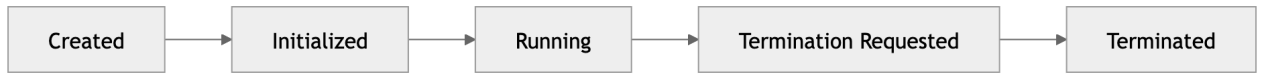
\includegraphics[width = 0.9\textwidth]{media/ameerapp1.png}
    \caption{Sensor Thread Lifecycle States}
    \label{fig-ameer1}
\end{figure}

\subsection{Initialization Phase of the Sensor Thread}
Following its creation, the sensor thread enters an initialization phase during which all thread-local resources and internal state variables are prepared. This phase establishes the foundation for safe and reliable operation throughout the runtime of the system.

Initialization includes preparing data structures used to temporarily store sensor values, verifying that utility-layer interfaces are accessible, and ensuring that the measurement device can be opened and accessed correctly. Any failure during this phase is treated as a critical condition, as continued execution without valid hardware access would lead to undefined system behavior or invalid measurement results. By performing these checks once during initialization rather than repeatedly during runtime, the implementation reduces overhead in the main execution loop and allows error conditions to be detected as early as possible.


\subsection{Transition into the Running State}
After successful initialization, the sensor thread transitions into its running state by entering a continuous execution loop. This loop constitutes the operational core of the sensor thread and remains active until a termination request is issued.

The loop-based execution model was selected deliberately over an interrupt-driven or event-based approach. While event-driven designs can be efficient under certain conditions, they often introduce additional complexity when deterministic periodic sampling is required. A loop-based model, by contrast, allows explicit control over sampling intervals, execution order, and timing behavior, which is particularly advantageous in measurement systems.

Each iteration of the loop corresponds to a single sampling cycle and is executed in a strictly sequential manner. This guarantees that all sensor values collected within one iteration represent a coherent snapshot of the system state.


\begin{figure}[H]
    \centering 
    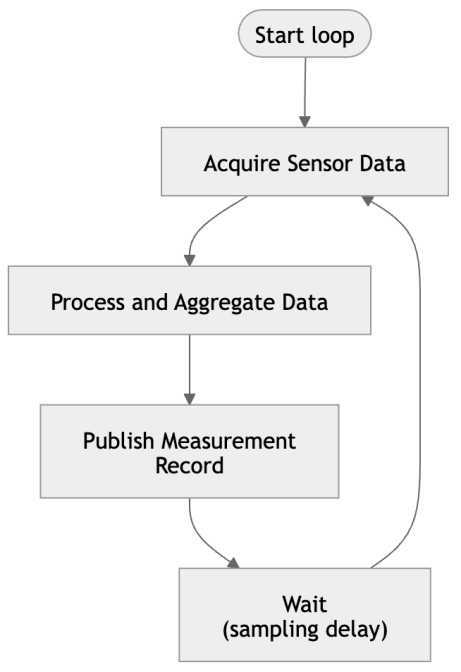
\includegraphics[scale = 0.7]{media/ameerapp3.png}
    \caption{High-Level Execution Flow of the Sensor Thread}
    \label{fig-ameer2}
\end{figure}

\subsection{Sensor Configuration Data Structure}


\begin{minted}[bgcolor = lightgray, tabsize = 4, breaklines]{c}
typedef struct
{
    sensor_id_t sid;
    uint32_t rate_hz;
    uint64_t period_us;
    uint64_t next_deadline;
    pthread_mutex_t lock;
} sensor_config_t;
\end{minted}

The behavior of the sensor thread is driven by a centralized configuration model that defines the runtime properties of each logical sensor. Each sensor is represented by a configuration structure containing its identifier, sampling rate, derived sampling period, and the next absolute deadline for acquisition. A dedicated mutex is associated with each configuration entry to allow safe runtime updates without interfering with ongoing sampling.

All sensor configurations are stored in a global array, enabling the sensor thread to iterate deterministically over all sensors within a single execution loop. This structure forms the foundation for the deadline-based scheduling mechanism described in the following sections and allows heterogeneous sensors to be managed uniformly within one thread.

\subsection{Structure of a Single Sampling Cycle}
Within each iteration of the execution loop, the sensor thread performs a fixed sequence of operations. The cycle begins with the acquisition of analog sensor values from the ADC subsystem, followed by the retrieval of digital switch states. These values are then combined into a unified measurement record representing the complete sensor state at that sampling instant.

The strict ordering of these operations is essential. By ensuring that analog and digital values are collected sequentially within the same loop iteration, the implementation avoids inconsistencies that could arise if different sensors were sampled at different times or under different system conditions.

Once all sensor values have been collected and assembled, the measurement record is handed over to a shared data structure, enabling other threads to access the data asynchronously.



\subsection{Management of Thread-Local State}
The sensor thread maintains several thread-local variables that persist across loop iterations. These variables store intermediate results such as raw ADC readings, decoded switch states, and aggregated measurement structures.

Thread-local storage plays a crucial role in simplifying concurrency control. Because these variables are not accessible to other threads, no synchronization is required during intermediate computation phases. Synchronization is only necessary when the final measurement record is published to shared memory, thereby minimizing the duration and frequency of critical sections.


\begin{table}[h]
    \centering
    \begin{tabular}{|l|l|l|}
        \hline
        \textbf{Category} & \textbf{Purpose} & \textbf{Lifetime} \\
        \hline
        Raw sensor values & Temporary storage of ADC and switch data & One loop iteration \\
        \hline
        Aggregated data & Complete measurement record & One loop iteration \\
        \hline
        Control flags & Execution and termination control & Thread lifetime \\
        \hline
    \end{tabular}
    \caption{Thread-Local State Categories in the Sensor Thread}
    \label{tab-ameer1}
\end{table}

\subsection{Interaction with Shared Resources}
From a concurrency standpoint, the sensor thread exclusively fulfills the role of a producer. It generates measurement data and publishes it to a shared buffer that is accessed by other server components. The sensor thread never consumes data from shared structures, which eliminates the possibility of circular dependencies or producer–producer conflicts.

The interaction with shared resources is deliberately confined to a narrowly defined section of the execution loop. This critical section is protected by synchronization mechanisms to guarantee atomicity and data consistency. Outside of this section, the sensor thread performs all computations without holding locks, thereby reducing contention and improving overall system responsiveness.

\begin{figure}[H]
    \centering 
    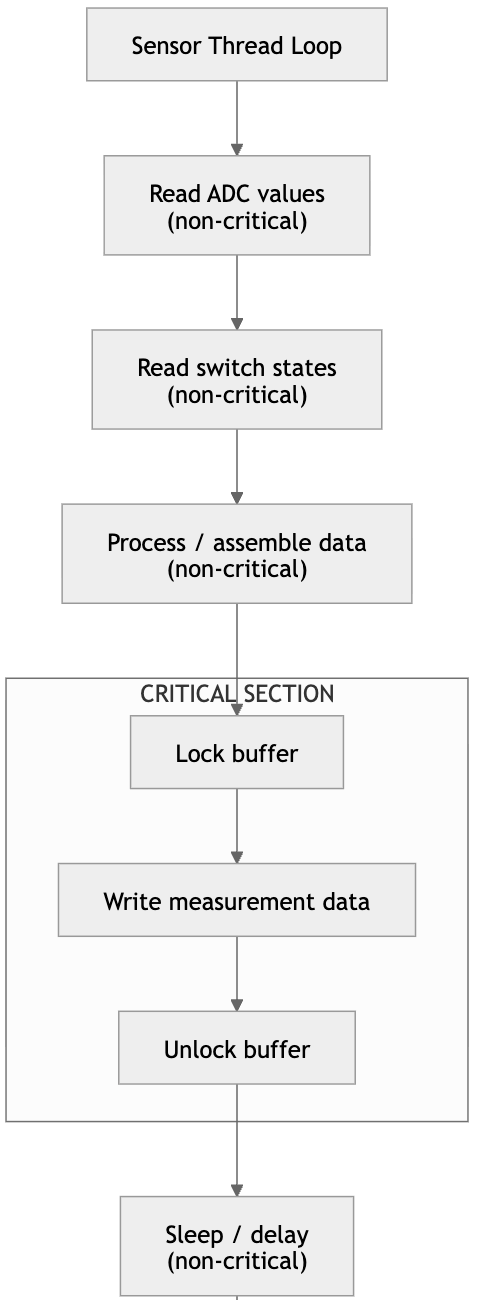
\includegraphics[scale = 0.7]{media/ameerapp4.png}
    \caption{Critical Section Placement within the Sensor Thread Loop}
    \label{fig-ameer3}
\end{figure}

\subsection{Timing Control and Sampling Period Regulation}
A key responsibility of the sensor thread is to regulate the sampling period. This is achieved by introducing an explicit delay at the end of each loop iteration. The delay duration defines the effective sampling rate and is selected based on expected sensor dynamics and system load considerations.

This approach provides a simple yet effective mechanism for controlling CPU utilization and ensuring predictable sampling behavior. While the system operates on a general-purpose Linux platform without hard real-time guarantees, the isolation of sensor acquisition into a dedicated thread allows for bounded timing variability and soft real-time behavior.


\subsection{Termination and Graceful Shutdown}
Termination of the sensor thread is initiated externally, typically as part of the overall server shutdown sequence. A shared termination flag or signal is used to inform the thread that execution should cease.

Rather than terminating immediately, the sensor thread completes its current sampling cycle before exiting the execution loop. This ensures that partially acquired data is not published and that shared resources are left in a consistent state. After exiting the loop, the thread releases any allocated resources and terminates cleanly.

\begin{figure}[H]
    \centering 
    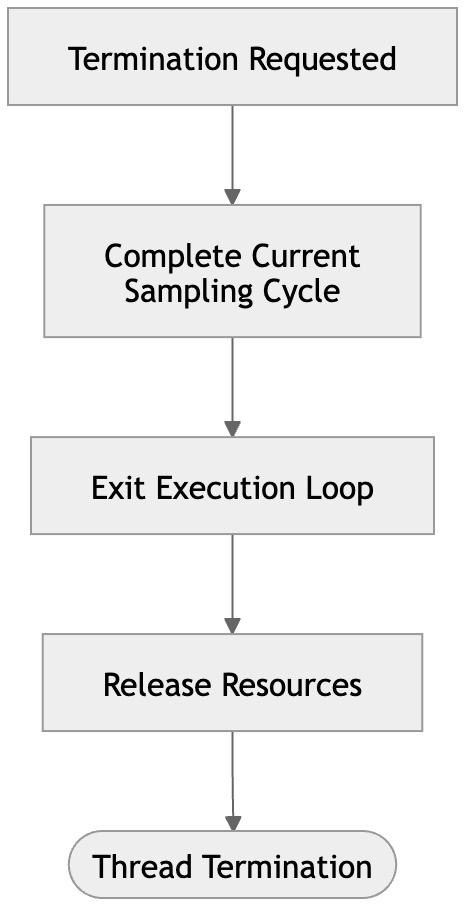
\includegraphics[scale = 0.5]{media/ameerapp5.png}
    \caption{Sensor Thread Shutdown Sequence}
    \label{fig-ameer4}
\end{figure}

\section{ADC Acquisition}
\subsection{Placement of ADC Acquisition in the Sensor Thread}
ADC acquisition is implemented entirely inside the sensor thread and is integrated into the thread’s deadline-driven main loop. The ADC logic is not isolated in a separate function; instead, it is embedded directly in the per-sensor handling switch–case structure. This design ensures that ADC acquisition follows the same scheduling and timestamping rules as all other sensors.

The ADC handling code is executed when the sensor identifier corresponds to either \texttt{adc\_zero\_sid} or \texttt{adc\_one\_sid}, as shown in the following excerpt from the sensor thread’s main loop.


\subsection{ADC-Related State Variables and Their Purpose}
Before examining the acquisition logic itself, it is important to understand the ADC-related state maintained by the sensor thread. These variables are declared at the beginning of the thread function:

\begin{minted}[bgcolor = lightgray, tabsize = 4, breaklines]{c}
static uint64_t last_adc_time = 0;
static unsigned int adc_zero_cache = 0, adc_one_cache = 0;
\end{minted}

These variables play a central role in the ADC acquisition strategy:

\begin{itemize}
    \item \texttt{last\_adc\_time} records the timestamp of the most recent ADC acquisition.
    \item \texttt{adc\_zero\_cache} and \texttt{adc\_one\_cache} store the most recently acquired ADC0 and ADC1 values.
\end{itemize}
The use of static storage duration ensures that these values persist across iterations of the sensor thread loop, allowing the ADC acquisition logic to coordinate multiple logical sensors within the same execution cycle.

\subsection{ADC Acquisition Logic in the Sensor Switch–Case}
The core ADC acquisition logic is implemented inside the switch–case statement that handles each sensor type. The following code block shows the complete ADC-related case handling exactly as implemented in \texttt{sensorThread.c:}

\begin{minted}[bgcolor = lightgray, tabsize = 4, breaklines]{c}
case adc_zero_sid:
case adc_one_sid:
    if (last_adc_time != now)
    {
        if (last_adc_time != now)
        {
            if (system_mode == MODE_SIM)
            {
                backend_read_adc(&adc_zero_cache, &adc_one_cache);
            }
            else
            {
                getADC(fd, &adc_zero_cache, &adc_one_cache);
            }

            last_adc_time = now;
        }
    }
    sample.sensor_value =
        (i == adc_zero_sid) ? adc_zero_cache : adc_one_cache;
    break;
\end{minted}
This block is the entire ADC acquisition mechanism of the server application. The design is compact but non-trivial, and each part serves a specific purpose.

\begin{minted}[bgcolor = lightgray, tabsize = 4, breaklines]{c}
if (last_adc_time != now)
\end{minted}

ensures that ADC acquisition is performed only once per scheduling instant. The variable now represents the current timestamp obtained from the high-resolution timer at the beginning of the loop iteration.

Because both ADC0 and ADC1 are processed sequentially within the same loop iteration, this condition prevents redundant ADC reads when the second logical ADC sensor is handled. Without this guard, the ADC hardware would be accessed twice per loop iteration, leading to unnecessary overhead and potential inconsistencies.

By tying ADC acquisition to the timestamp rather than to the sensor ID, the implementation guarantees that both ADC channels correspond to the same physical sampling instant.

\subsection{Simulation Mode ADC Acquisition}
Within the ADC acquisition block, the first distinction made is between simulation mode and real hardware mode:
\subsection{Timestamp-Based Synchronization of ADC Channels}
The outer condition:
\begin{minted}[bgcolor = lightgray, tabsize = 4, breaklines]{c}
if (system_mode == MODE_SIM)
{
    backend_read_adc(&adc_zero_cache, &adc_one_cache);
}
\end{minted}
In simulation mode, ADC values are generated by the \texttt{backend\_read\_adc()} function. This function provides synthetic ADC values that emulate real sensor behavior. Importantly, the simulation function writes both ADC channel values at once, matching the behavior expected from real hardware.

This design ensures that:
\begin{itemize}
    \item Simulation mode exercises the same caching, scheduling, and buffering logic as real hardware mode.

    \item Downstream components such as the ring buffer and network thread are completely unaware of whether ADC values originate from hardware or simulation.
\end{itemize}
Simulation mode therefore acts as a drop-in replacement for real ADC hardware during development, testing, and debugging.

\subsection{Hardware ADC Acquisition}
When the system is operating in real hardware mode, ADC acquisition is performed using the following call:

\begin{minted}[bgcolor = lightgray, tabsize = 4, breaklines]{c}
getADC(fd, &adc_zero_cache, &adc_one_cache);
\end{minted}
This function reads both ADC0 and ADC1 values from the hardware through the \texttt{/dev/meascdd} character device. The file descriptor fd was previously opened during sensor thread initialization and represents the user-space interface to the measurement hardware implemented in the Zynq programmable logic.

The combined ADC read approach ensures that:
\begin{itemize}
    \item Both channels are sampled during the same conversion cycle.

    \item Hardware access overhead is minimized.

    \item Channel synchronization is enforced at the acquisition level.
\end{itemize}
All time-critical operations such as SPI signaling and conversion timing are handled in hardware, while the sensor thread performs synchronous access to retrieve the completed conversion results.

\subsubsection{Measurement Device Interface for ADC Access}
Access to the ADC hardware from user space is mediated through a custom Linux character device, /dev/meascdd. The interface to this device is defined in measdev.h, which specifies the data structures and constants used for all measurement-related hardware communication. This interface forms the software–hardware boundary between the sensor thread running on the ARM processing system and the measurement logic implemented in the Zynq programmable logic.

\begin{figure}[H]
    \centering 
    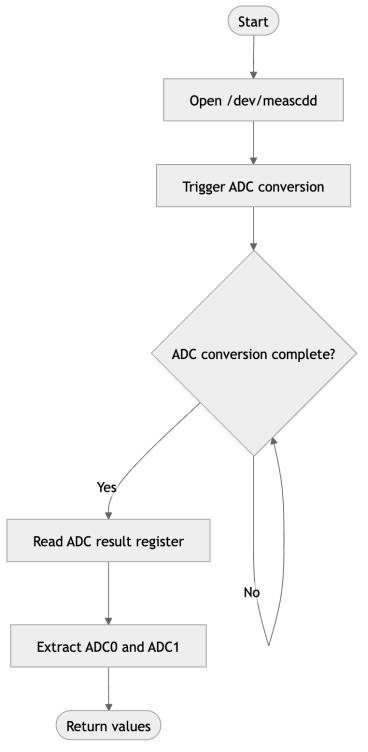
\includegraphics[scale = 1.3]{media/ameerapp6.png}
    \caption{ADC acquisition control flow}
    \label{fig-ameer5}
\end{figure}

At the core of this interface is the register object structure:
\begin{minted}[bgcolor = lightgray, tabsize = 4, breaklines]{c}
typedef struct
{
    unsigned int rnum;
    unsigned int rvalue;
} measObj_struct;
\end{minted}
Each interaction with the measurement hardware is expressed as a register-oriented transaction, where rnum identifies the target register and rvalue carries either control information or returned data. These structures are transferred atomically between user space and the kernel module using standard \texttt{read()} and \texttt{write()} system calls. The fixed size of the structure, defined by \texttt{MEASOBJ\_SIZE}, ensures deterministic and aligned communication.

The measdev interface defines symbolic identifiers such as \texttt{REGNUM\_ID} to distinguish register access operations. During ADC acquisition, these identifiers are used by the utility function getADC() to initiate a conversion, poll conversion status, and retrieve the combined ADC result register. The details of register addresses and bit-level signaling remain encapsulated within the kernel module and FPGA logic, while the user-space code operates exclusively through the abstracted register interface.

This design allows the sensor thread to remain independent of hardware-specific implementation details. The ADC acquisition logic described earlier focuses on scheduling, synchronization, and data flow, while measdev provides a consistent and reusable communication contract. The same interface is later reused for switch and push button access, reinforcing a unified hardware abstraction across the server application.

\subsection{Cache Update and Acquisition Timestamping}
After either simulation or real hardware acquisition, the ADC cache and timestamp are updated:

\begin{minted}[bgcolor = lightgray, tabsize = 4, breaklines]{c}
last_adc_time = now;
\end{minted}
This assignment marks the completion of ADC acquisition for the current loop iteration. Subsequent processing of the second ADC logical sensor within the same iteration will reuse the cached values instead of triggering a new hardware read.

This mechanism is essential for maintaining consistent behavior when multiple logical sensors share a single physical acquisition process.

\subsection{Mapping Cached ADC Values to Logical Samples}
Once ADC values are available in the cache, the sensor thread assigns the appropriate value to the current sample:

\begin{minted}[bgcolor = lightgray, tabsize = 4, breaklines]{c}
sample.sensor_value =
    (i == adc_zero_sid) ? adc_zero_cache : adc_one_cache;
\end{minted}
This line maps the physical ADC values to logical sensor samples. Each ADC channel produces its own \texttt{sensor\_data\_t} structure, containing:

\begin{itemize}
    \item A unique sensor identifier
    \item A timestamp corresponding to the acquisition instant
    \item A channel-specific digital value
\end{itemize}
Although ADC0 and ADC1 share a single acquisition operation, they are treated as independent data streams once inserted into the ring buffer.

\subsection{Integration with the Ring Buffer}
After the ADC value has been assigned, the sample is published to the shared ring buffer:

\begin{minted}[bgcolor = lightgray, tabsize = 4, breaklines]{c}
ringBufferAddSample(rb, &sample);
\end{minted}
This marks the end of ADC handling for the current sensor. From this point onward, the sensor thread no longer interacts with the ADC data. The ring buffer acts as the boundary between data acquisition and data transmission.

The network thread later consumes these samples and transmits them to connected clients, ensuring a clean producer–consumer separation between acquisition and communication.

\begin{figure}[H]
    \centering 
    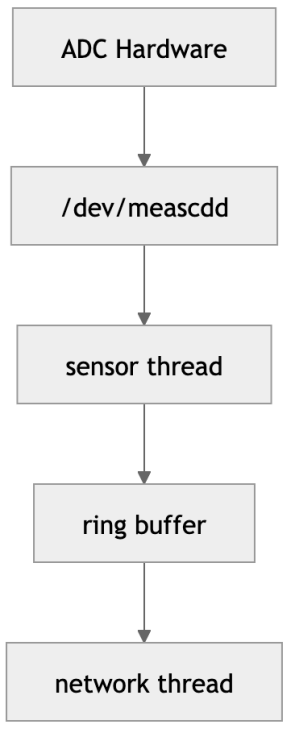
\includegraphics[scale = 0.8]{media/ameerapp7.png}
    \caption{ADC Data Flow in Sensor Thread}
    \label{fig-ameer7}
\end{figure}

\subsection{Timing Characteristics of ADC Acquisition}
ADC acquisition is synchronized with the sensor thread’s deadline-based scheduling framework. Because ADC reads occur only when the sensor deadline is reached and only once per loop iteration, the execution time overhead introduced by ADC acquisition is bounded and predictable.

This predictability is crucial in a Linux-based system where strict real-time guarantees are not available. By delegating time-critical conversion tasks to the programmable logic and limiting user-space interaction to synchronized reads, the design achieves deterministic behavior suitable for measurement applications.

\subsection{Robustness and Failure Containment}
The ADC acquisition logic is structured so that failures do not propagate beyond the sensor thread. If ADC acquisition fails or returns invalid data, only the affected sample is impacted. Other sensors continue to operate normally, and the server remains responsive.

This localized failure containment contributes to the overall robustness of the Measurement Network Gateway and ensures continued operation under adverse conditions.


\subsection{ADC Hardware Access Implementation}
While the sensor thread determines when ADC acquisition is performed, the actual mechanism for retrieving ADC values from the hardware is implemented in the utility layer. This separation of responsibilities allows the sensor thread to concentrate on scheduling, synchronization, and data flow, while low-level register access and hardware interaction are encapsulated in a dedicated module. As a result, changes to the hardware interface or register mapping can be handled locally within the utility layer without affecting higher-level logic.

The ADC hardware access is implemented by the \texttt{getADC()} function in \texttt{utils.c}. This function communicates with the Zynq programmable logic through the /dev/meascdd character device, which exposes the measurement registers implemented in the FPGA fabric to user-space software running on the processing system.

\subsubsection{Overview of the ADC Access Strategy}
The ADC subsystem provides two conversion channels, corresponding to ADC0 and ADC1. These channels are acquired together as part of a single conversion sequence, ensuring that both analog inputs are sampled at the same instant. This synchronized acquisition is particularly important when the ADC channels are used to observe related or correlated signals.

The \texttt{getADC()} function implements a structured acquisition sequence in which a conversion is first triggered in the hardware, after which the function repeatedly polls the conversion status until completion. Once the hardware indicates that valid conversion data is available, the combined ADC result register is read. This register contains the digital representations of both ADC channels, which are then separated into individual values and returned to the caller via pointer arguments.

By performing ADC acquisition in this manner, the implementation achieves deterministic behavior while keeping the user-space code simple and robust. All timing-critical operations are handled within the programmable logic, and the utility layer provides a clean, synchronous interface for higher-level software components.

\subsubsection{ADC Conversion Trigger and Status Polling}
The ADC acquisition begins by initiating a conversion through a register write:

\begin{minted}[bgcolor = lightgray, tabsize = 4, breaklines]{c}
void getADC(int fd, unsigned int *adc_zero, unsigned int *adc_one)
{
    int ccount;
    unsigned int xstatus, adc_lZero, adc1_lOne;

    tf_obj_snd.rnum = 4; // start conversion
    tf_obj_snd.rvalue = 0;
    write(fd, &tf_obj_snd, MEASOBJ_SIZE);
\end{minted}

Here, the \texttt{tf\_obj\_snd} structure is populated with a register number corresponding to the ADC control register. Writing this structure to \texttt{/dev/meascdd} triggers the programmable logic to start a conversion sequence.

Immediately after triggering the conversion, the function enters a polling loop:

\begin{minted}[bgcolor = lightgray, tabsize = 4, breaklines]{c}
    ccount = 0;
        do
        {
            ccount++;
            read(fd, &tf_obj_rcv, MEASOBJ_SIZE); // Read response from LKM
            xstatus = tf_obj_rcv.rvalue;
        } while ((xstatus == 0) && (ccount < 10000000));
\end{minted}

This loop repeatedly reads the ADC status register until the conversion is complete or a timeout threshold is reached. The polling approach ensures that the function only proceeds once valid conversion data is available, while the loop counter prevents indefinite blocking in case of hardware malfunction.

\subsubsection{Reading and Decoding ADC Result Registers}
Once conversion completion is detected, the function requests the ADC result register:

\begin{minted}[bgcolor = lightgray, tabsize = 4, breaklines]{c}
   tf_obj_snd.rnum = REGNUM_ID;
    tf_obj_snd.rvalue = 5; // ADC status register
    write(fd, &tf_obj_snd, MEASOBJ_SIZE);
    read(fd, &tf_obj_rcv, MEASOBJ_SIZE); // Read response
\end{minted}

The returned register value contains the results of both ADC channels packed into a single 32-bit word. The lower and upper portions of this word correspond to ADC0 and ADC1 respectively.

The function then extracts the individual channel values using bitwise operations:


\begin{minted}[bgcolor = lightgray, tabsize = 4, breaklines]{c}
    adc1_lOne = tf_obj_rcv.rvalue;
        adc_lZero = adc1_lOne & 0x0fff;
        adc1_lOne >>= 16;

        *adc_zero = adc_lZero;
        *adc_one = adc1_lOne;
    }
\end{minted}

\subsubsection{Interaction with the Sensor Thread}
The getADC() function is invoked by the sensor thread as part of the ADC acquisition process. During each scheduled acquisition cycle, the sensor thread calls this function to retrieve the most recent ADC conversion results from the hardware. The function returns both ADC channel values through pointer arguments, allowing the sensor thread to store the results in local cache variables. These cached values are subsequently assigned to logical sensor samples and incorporated into the standard data flow used for all sensors.

This interaction establishes a clear division of responsibilities between the sensor thread and the utility layer. The sensor thread remains agnostic to hardware-specific details and focuses solely on scheduling, synchronization, and data handling. At the same time, the utility layer encapsulates all register-level communication and hardware semantics, ensuring that any changes to ADC register mapping or access mechanisms can be confined to utils.c without affecting higher-level logic.

\subsubsection{Design Considerations and Advantages}
The ADC utility implementation provides a structured and efficient approach to hardware access within the Measurement Network Gateway. By acquiring both ADC channels in a single operation, the design guarantees synchronized dual-channel sampling while avoiding redundant hardware access. The user-space logic required to retrieve ADC data is kept intentionally minimal, reducing complexity in the sensor thread and improving maintainability.

This separation between scheduling logic and hardware access contributes to a clean architectural design in which timing-critical operations are handled within the programmable logic, while user-space software performs deterministic, synchronous access to completed conversion results. The same register-based access pattern is reused across multiple hardware interfaces, including switches and push buttons, reinforcing consistency and modularity throughout the server implementation.


\section{Switch Handling}
\subsection{Role of Switch Inputs in the Measurement Network Gateway}
Slide switches on the ZedBoard provide persistent digital input states that can be used to represent configuration settings, operating modes, or user-defined flags during system operation. Unlike push buttons, which generate momentary events, slide switches maintain a stable ON or OFF state until manually changed by the user. This makes them particularly suitable for representing long-lived system conditions that should be sampled periodically rather than edge-triggered.

In the Measurement Network Gateway, slide switches are treated as digital sensors and are integrated into the same acquisition, buffering, and transmission pipeline as analog inputs. Their states are sampled by the sensor thread at a fixed rate, timestamped, and forwarded to the ring buffer for subsequent transmission to connected clients.

\subsection{Switch Acquisition in the Sensor Thread}
Switch acquisition is implemented directly within the sensor thread’s main scheduling loop. The acquisition logic is selected based on the sensor identifier corresponding to slide switches. The complete switch-handling logic in sensorThread.c is shown below:

\begin{minted}[bgcolor = lightgray, tabsize = 4, breaklines]{c}
case sw_sid:
    if (system_mode == MODE_SIM)
        sample.sensor_value = backend_read_switches();
    else
        sample.sensor_value = readZedSwitches(fd);
    break;
\end{minted}

This code illustrates that switch handling follows the same architectural pattern as other sensors. In simulation mode, synthetic switch values are generated by a backend function, allowing the server and network stack to be tested without hardware. In real hardware mode, the sensor thread retrieves the current switch states using a dedicated utility-layer function.

The acquired switch value is stored directly in the sensor\_value field of the sample structure and is subsequently processed in the same way as all other sensor data.

\subsection{Scheduling and Timing Characteristics of Switch Sampling}
Switch sampling is governed by the same deadline-based scheduling mechanism used for all sensors. Each switch sensor entry has an associated sampling period and next-deadline timestamp stored in the sensor configuration structure. When the current time exceeds the deadline, the sensor thread reads the switch state and generates a new sample.

Because slide switch states change relatively infrequently and switch read operations are fast and non-blocking, periodic polling is an efficient and reliable acquisition strategy. The execution time of switch reads is negligible compared to analog sensor acquisition, ensuring that switch sampling does not interfere with higher-frequency sensors such as ADC channels.

\subsection{Switch Hardware Access in the Utility Layer}
The actual interaction with ZedBoard switch hardware is implemented in the utility layer within the \texttt{readZedSwitches()} function. This function abstracts the low-level register access required to retrieve the current switch states from the programmable logic.

The complete implementation of the switch access function in utils.c is shown below:
\begin{minted}[bgcolor = lightgray, tabsize = 4, breaklines]{c}
unsigned int readZedSwitches(int fd)
{
    tf_obj_snd.rnum = REGNUM_ID;
    tf_obj_snd.rvalue = 0;

    write(fd, &tf_obj_snd, MEASOBJ_SIZE);
    read(fd, &tf_obj_rcv, MEASOBJ_SIZE);

    return (tf_obj_rcv.rvalue) & 0xff;
}
\end{minted}

The function constructs a register access request using the \texttt{measObj\_struct }defined in measdev.h. The request is sent to the kernel module via a \texttt{write()} system call, and the response is retrieved using a corresponding \texttt{read()} call. The returned register value contains the digital states of multiple inputs packed into a single 32-bit word.

By masking the lower eight bits of the returned value, the function extracts the states of the slide switches and returns them as an 8-bit value to the caller. Each bit corresponds to the state of a physical switch, with a value of 1 indicating an ON position and 0 indicating OFF.

\subsection{Switch State Encoding and Interpretation}
The slide switch states are represented as a compact bit field, allowing all switch positions to be conveyed using a single integer value. Each bit in the returned value corresponds to one physical switch on the ZedBoard. This encoding enables efficient transmission and straightforward interpretation by downstream components.

\begin{table}[h]
    \centering
    \begin{tabular}{|l|l|l|}
        \hline
        \textbf{Switch Index} & \textbf{Bit Position} & \textbf{Description} \\
        \hline
        SW0 & Bit 0 & Slide switch 0 \\
        \hline
        SW1 & Bit 1 & Slide switch 1 \\
        \hline
        SW2 & Bit 2 & Slide switch 2 \\
        \hline
        SW3 & Bit 3 & Slide switch 3 \\
        \hline
        SW4 & Bit 4 & Slide switch 4 \\
        \hline
        SW5 & Bit 5 & Slide switch 5 \\
        \hline
        SW6 & Bit 6 & Slide switch 6 \\
        \hline
        SW7 & Bit 7 & Slide switch 7 \\
        \hline
    \end{tabular}
    \caption{ZedBoard Slide Switch Encoding}
\end{table}

This representation allows multiple switch states to be sampled, buffered, and transmitted as a single sensor value, minimizing overhead while preserving complete state information.


\subsection{Integration with the Measurement Device Interface }
Switch acquisition relies on the same measurement device interface (measdev) used for ADC and other sensors. The register-based communication model ensures a consistent and unified hardware abstraction across all input types. By routing switch access through the measdev interface, the server software remains insulated from hardware-specific implementation details such as GPIO wiring or FPGA register layout.

This unified interface simplifies maintenance and ensures that modifications to the hardware design or register mapping can be handled within the kernel module and utility layer without impacting the sensor thread logic.

\subsection{Data Flow from Switch Hardware to Network Transmission}
Once the switch value has been retrieved by the utility layer, it is incorporated into a \texttt{sensor\_data\_t} structure by the sensor thread along with the current timestamp and sensor identifier. The sample is then inserted into the shared ring buffer, where it becomes available to the network thread.

The network thread later retrieves buffered samples and transmits them to connected clients. From the perspective of the communication layer and the graphical user interface, switch data is handled identically to other sensor types, enabling unified visualization and analysis.

\begin{figure}[H]
    \centering 
    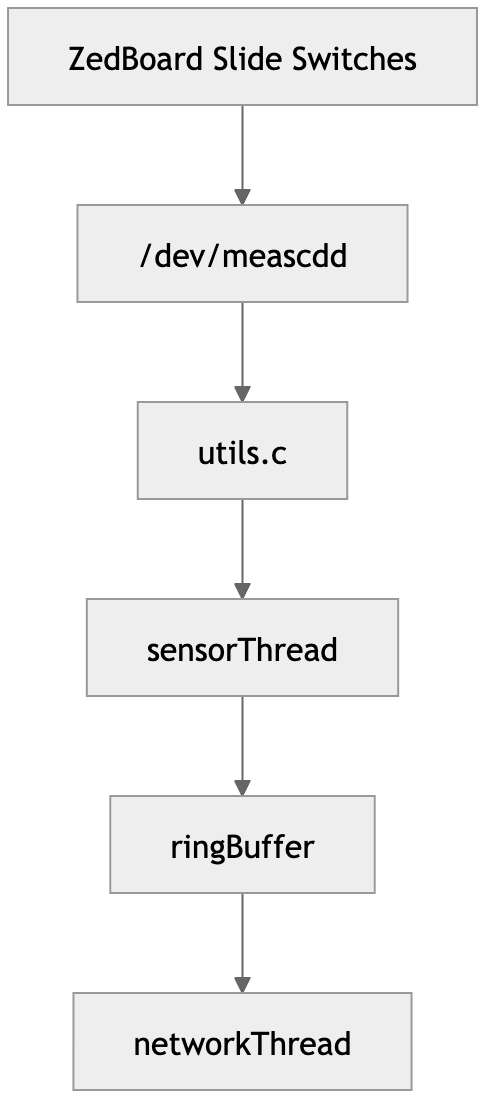
\includegraphics[scale = 0.7]{media/ameerapp8.png}
    \caption{Switch Data Flow through the Server}
    \label{fig-ameer8}
\end{figure}

\section{Utility Layer Analysis}
\subsection{Purpose of the Utility Layer}
The utility layer serves as the hardware abstraction and timing service component of the Measurement Network Gateway server. Its primary purpose is to isolate low-level hardware interaction and platform-specific functionality from the higher-level application logic implemented in the sensor thread. By centralizing these responsibilities, the utility layer enables a clear separation between what the system measures and how those measurements are obtained from the hardware.

This design reduces complexity in the sensor thread and ensures that hardware-specific details do not propagate into scheduling, buffering, or networking code.

\subsection{Abstraction of Hardware Interaction}
All direct interaction with the measurement hardware is performed through the utility layer. This includes access to ADC channels and slide switch states via the register-based interface exposed by the Linux kernel module. The sensor thread invokes utility functions to retrieve measurement values without requiring knowledge of register identifiers, bit layouts, or communication protocols.

This abstraction ensures that changes to the hardware implementation, such as modified register mappings or alternative peripherals, can be accommodated by modifying the utility layer alone. The rest of the server software remains unaffected, improving maintainability and extensibility.

\subsection{Support for Deterministic Timing}
In addition to hardware access, the utility layer provides a unified timing service based on a monotonic clock source. This timing service establishes a common reference for all sensor acquisitions and enables consistent timestamping across different sensor types.

By centralizing timing functionality, the design avoids redundant or inconsistent time calculations and ensures that all scheduling decisions made by the sensor thread are based on a stable and reliable time base. This is particularly important in a Linux environment, where system time adjustments must not affect measurement consistency.

\subsection{Consistency across Sensor Types}
Although different sensors exhibit different acquisition characteristics, the utility layer presents a consistent interaction model to the sensor thread. ADC channels, slide switches, and other inputs are accessed through uniform function calls that return ready-to-use values. The sensor thread therefore applies the same scheduling, timestamping, and buffering logic to all sensor data.

This consistency simplifies the overall system design and reinforces the modular architecture of the server. It also allows simulation mode and real hardware mode to be handled transparently at the sensor thread level.

\subsection{Interaction with Higher-Level Components}
The utility layer does not interact directly with the ring buffer or the network thread. Instead, it functions as a service provider to the sensor thread, which acts as the central coordinator of data acquisition and data flow. This strict layering prevents low-level code from becoming entangled with application-level concerns such as batching, serialization, or network transmission.

As a result, the server architecture remains cleanly layered, with well-defined responsibilities assigned to each component.

\subsection{Maintainability and Design Implications}
By encapsulating hardware access and timing services within a dedicated module, the utility layer significantly improves the maintainability of the Measurement Network Gateway. The sensor thread logic remains compact and readable, while hardware-specific complexity is localized in a single place.

This design choice supports long-term extensibility and aligns with best practices for embedded and real-time software systems, where clear abstraction boundaries are essential for reliability and scalability.


\section{Timing and Determinism}
\subsection{Motivation for Deterministic Timing in the Server}
The Measurement Network Gateway operates in a Linux user-space environment, which does not provide hard real-time guarantees. Nevertheless, predictable and repeatable timing behavior is essential for meaningful sensor data acquisition, particularly when correlating analog measurements, digital inputs, and external stimuli. The server design therefore emphasizes bounded execution time, consistent timestamping, and controlled scheduling rather than strict real-time determinism.

The timing strategy is implemented primarily within the sensor thread and is supported by the utility layer’s monotonic timing services. Together, these components provide a deterministic acquisition framework that is robust against operating system scheduling variability.

\subsection{Monotonic Time Base and Timestamp Consistency}
All timing decisions in the server are based on a monotonic clock source. During initialization, the utility layer establishes a reference time using CLOCK\_MONOTONIC, which is immune to system time adjustments such as NTP corrections or manual clock changes.

\begin{minted}[bgcolor = lightgray, tabsize = 4, breaklines]{c}
void initTimer(void)
{
    struct timespec ts;
    clock_gettime(CLOCK_MONOTONIC, &ts);
    us_startup_time = ts.tv_sec * 1000000 + ts.tv_nsec / 1000;
}
\end{minted}

Subsequent calls to getElapsedTime() return the elapsed time in microseconds relative to this startup reference. This approach ensures that all timestamps are strictly increasing and comparable across the lifetime of the server process.

\begin{minted}[bgcolor = lightgray, tabsize = 4, breaklines]{c}
uint64_t getElapsedTime(void)
{
    clock_gettime(CLOCK_MONOTONIC, &current_time);
    return (current_time.tv_sec * 1000000 + current_time.tv_nsec / 1000)
           - us_startup_time;
}
\end{minted}

By centralizing timestamp generation in the utility layer, the system avoids inconsistencies that could arise from multiple time sources or mixed clock domains.

\subsection{Deadline-Based Sensor Scheduling}
Deterministic sampling behavior is achieved through a deadline-based scheduling mechanism implemented in the sensor thread. Each sensor is associated with a sampling period and a next-deadline timestamp, which together define when acquisition should occur.

At runtime, the sensor thread continuously compares the current time against each sensor’s deadline:
\begin{minted}[bgcolor = lightgray, tabsize = 4, breaklines]{c}
if (now >= sensor_cfg[i].next_deadline)
{
    /* acquire sensor and create sample */
}
\end{minted}

This condition ensures that sensor acquisition is triggered only when the configured sampling period has elapsed. Importantly, the comparison is based on absolute time rather than relative delays, which prevents cumulative drift over long execution periods.

\subsection{Deadline Catch-Up and Overrun Handling}
After a sensor sample has been acquired, the deadline is advanced using a catch-up loop:

\begin{minted}[bgcolor = lightgray, tabsize = 4, breaklines]{c}
while (now >= sensor_cfg[i].next_deadline)
    sensor_cfg[i].next_deadline += sensor_cfg[i].period_us;
\end{minted}

This mechanism ensures that missed deadlines do not permanently shift the sampling schedule. If the sensor thread experiences a temporary delay due to operating system scheduling or transient load, the loop advances the deadline until it lies in the future. As a result, the system resumes sampling aligned with the original schedule rather than accumulating phase error.

This approach is particularly important in a Linux environment, where short scheduling delays are unavoidable but should not compromise long-term timing stability.


\subsection{Bounded Execution Time within the Sensor Thread}
Determinism in the server is further supported by bounding the execution time of the sensor thread loop. Hardware interaction is deliberately limited to synchronous register reads that complete quickly and predictably. Time-critical operations such as ADC conversion timing and SPI signaling are delegated to the programmable logic, ensuring that user-space execution time remains bounded.

Additionally, the sensor thread includes a short sleep at the end of each iteration:

\begin{minted}[bgcolor = lightgray, tabsize = 4, breaklines]{c}
usleep(50);
\end{minted}

This delay is chosen to be significantly shorter than the smallest sampling period used in the system. It reduces CPU load and prevents busy-waiting, while still allowing the thread to respond promptly to upcoming deadlines.

\subsection{Deterministic Handling of Multi-Channel Sensors}
For sensors that share a common acquisition mechanism, such as the two ADC channels, deterministic behavior is ensured by synchronizing acquisition at the timestamp level. A single acquisition operation is performed per scheduling instant, and the resulting values are reused for multiple logical sensors. This guarantees that both channels correspond to the same physical sampling time and eliminates race conditions or inconsistent readings.

By anchoring multi-channel acquisition to a single timestamp, the system maintains internal consistency even when operating under non-real-time scheduling conditions.


\subsection{Interaction with Linux Scheduling}
Although the server runs under a general-purpose Linux scheduler, its design minimizes sensitivity to scheduling jitter. Absolute-time deadlines, monotonic timestamps, and bounded execution paths ensure that short delays do not propagate into long-term timing errors.

The system does not attempt to enforce hard real-time constraints. Instead, it provides soft real-time behavior that is sufficient for measurement and monitoring applications. This design choice balances predictability with portability and simplifies deployment on standard Linux systems without requiring real-time patches.


\section{Design Alternatives}
\subsection{Rationale for Discussing Design Alternatives}
The Measurement Network Gateway server was designed with a strong emphasis on modularity, predictability, and portability within a Linux user-space environment. While the chosen architecture meets the functional and timing requirements of the project, several alternative design approaches were considered during development. This section discusses those alternatives and explains why the final design was selected over other possible implementations.

The discussion focuses on sensor acquisition timing, threading model, hardware access strategy, and operating system interaction, all of which have a direct impact on determinism and system complexity.

\subsection{Polling-Based Scheduling versus Timer-Driven Acquisition}
One alternative to the implemented deadline-based scheduling approach is a purely timer-driven design, in which each sensor acquisition is triggered by a periodic timer using functions such as usleep(period) or POSIX interval timers.

In a simple timer-driven model, each sensor would block for a fixed duration and then perform acquisition. While this approach is easy to implement, it suffers from cumulative drift when execution time varies or when the thread is preempted by the operating system. Over long runtimes, such drift can significantly distort sampling intervals.

The chosen design avoids this issue by using absolute-time deadlines based on a monotonic clock. Instead of sleeping for a fixed duration, the sensor thread compares the current time against a precomputed deadline and advances that deadline explicitly after each acquisition. This approach prevents long-term phase drift and ensures that short scheduling delays do not permanently alter sampling behavior.

\subsection{Relative Delays versus Absolute Deadlines}
Another design alternative would be to use relative delays between acquisitions, for example by sleeping for the sensor’s sampling period after each acquisition. This approach is commonly used in simpler embedded systems but is less suitable in a preemptive multitasking environment such as Linux.

In contrast, the implemented design uses absolute deadlines derived from a monotonic time base. After each acquisition, the deadline is advanced until it lies in the future, effectively compensating for any missed periods. This strategy allows the system to recover gracefully from temporary overload or scheduling jitter without accumulating timing error.

This choice directly supports the system’s determinism goals while remaining compatible with standard Linux scheduling behavior.

\subsection{Single-Threaded versus Multi-Threaded Sensor Tasks}
An alternative architectural approach would be to assign each sensor its own dedicated thread. In such a design, each thread would manage its own timing and hardware access independently. While this can simplify per-sensor logic, it introduces additional complexity in terms of thread management, synchronization, and scheduling overhead.

The chosen single sensor-thread design avoids these issues by centralizing all acquisition logic in one controlled execution context. This reduces the number of threads contending for CPU time and simplifies synchronization with shared resources such as the ring buffer. It also ensures that all sensors share a common time base and scheduling framework, which is particularly important for correlating measurements across sensor types.

\subsection{User-Space versus Kernel-Space Acquisition}
Another possible design alternative would be to perform sensor acquisition entirely within kernel space by extending the Linux device driver. This could offer tighter timing control and reduced context-switch overhead. However, kernel-space implementations are more complex to develop, harder to debug, and less portable.

The chosen user-space acquisition model strikes a balance between determinism and maintainability. Time-critical operations such as ADC conversion timing and SPI signaling are delegated to the programmable logic, while user-space software performs synchronized access to completed measurements. This separation leverages the strengths of both hardware and software without introducing unnecessary kernel complexity.

\subsection{Wall-Clock Time versus Monotonic Time Sources}
Another design decision concerns the choice of time source. Using wall-clock time functions such as \texttt{time()} or \texttt{gettimeofday()} would allow timestamps to reflect real-world time, but these functions are vulnerable to discontinuities caused by system time adjustments.

The implemented design instead relies on a monotonic clock source, ensuring that timestamps are strictly increasing and immune to external time corrections. This choice is particularly important for timing analysis, debugging, and correlating sensor data over long execution periods.

\subsection{Real-Time Linux Extensions versus Soft Real-Time Design}
The system could also have been implemented using real-time Linux extensions, such as the \texttt{PREEMPT\_RT} patch or real-time scheduling policies. While these approaches can improve timing guarantees, they introduce additional system configuration requirements and reduce portability.

The selected design adopts a soft real-time approach that achieves sufficient determinism through careful scheduling, bounded execution time, and hardware-assisted acquisition. This allows the system to run reliably on standard Linux distributions without specialized kernel support, which aligns with the educational and experimental goals of the project.

\section{Testing and Fault Analysis}
\subsection{Objectives of Testing and Validation}
The objective of testing in the Measurement Network Gateway server is to verify that the implemented acquisition architecture behaves correctly under normal operating conditions and remains stable under abnormal or degraded scenarios. Testing focuses on functional correctness, timing consistency, robustness against faults, and graceful degradation when parts of the system are stressed or unavailable.

Rather than validating individual functions in isolation, the testing strategy evaluates the complete acquisition chain, from hardware interaction through user-space processing to buffered data delivery. This approach reflects the real operational environment of the gateway and ensures that design assumptions made in earlier sections hold under practical conditions.


\subsection{Functional Validation of Sensor Acquisition}
Functional testing confirms that each sensor type produces correct and consistent data when accessed through the server. For ADC channels, known analog input signals are applied, and the resulting digital values are compared against expected ranges. Switch inputs are validated by toggling physical switches and observing corresponding changes in reported values.

Correct operation is defined not only by accurate readings, but also by correct timestamp assignment and consistent sample publication into the ring buffer. Successful functional validation demonstrates that the separation between acquisition logic, utility layer, and buffering does not introduce data corruption or misalignment.


\subsection{Timing Validation and Sampling Consistency}
Timing behavior is a critical aspect of the server design. Validation focuses on ensuring that sensor sampling adheres to the configured rates and that timestamp differences between consecutive samples remain bounded.

While Linux does not provide hard real-time guarantees, the deadline-based scheduling strategy is expected to limit jitter to acceptable levels. Timing validation is therefore performed by analyzing inter-sample intervals derived from recorded timestamps.


\subsection{Robustness Against Partial Failures}
The server is designed so that failures in one sensor path do not affect others. ADC acquisition, switch handling, and timestamp generation are independent at the logical level, even though they share the same scheduling thread. This isolation ensures that an error in one acquisition path does not block or stall the entire system.

For example, if ADC acquisition experiences increased latency due to hardware delay, switch sampling and timestamp generation continue unaffected. This robustness is particularly important in mixed-sensor environments where not all sensors have identical timing or reliability characteristics.


\subsection{Validation of Hardware–Software Boundary}
Testing also validates the interface between user-space software and the kernel-level measurement device. Register reads and writes are verified to produce consistent results, and repeated access does not lead to stale or inconsistent data.

By treating the device interface as a black box during testing, the server software is validated against realistic hardware behavior rather than idealized assumptions. This approach increases confidence that the system will behave correctly even if the underlying hardware implementation changes, as long as the register contract is preserved.

\subsection{Observability and Debug Support}
The inclusion of timestamps and structured sensor samples significantly improves observability during testing. Logged output and networked data streams allow developers to correlate sensor values with acquisition times and identify anomalies such as missed deadlines or unexpected delays.

This observability makes it possible to diagnose performance issues without invasive instrumentation or intrusive debugging techniques, which is particularly valuable in timing-sensitive systems.


\subsection{Conclusion}
This work presented the design and implementation of the server-side acquisition software for the Measurement Network Gateway. The focus was placed on sensor data acquisition, timing control, and hardware abstraction, with particular emphasis on ADC sampling and switch handling.

A deadline-based scheduling approach was employed to achieve predictable sampling behavior in a Linux user-space environment. By using a monotonic time base and absolute deadlines, the system avoids long-term drift and limits timing jitter without relying on real-time kernel extensions. Time-critical conversion and signaling tasks are delegated to programmable logic, while user-space software performs synchronized access to completed measurements.

The implementation demonstrates a clear separation of concerns between scheduling, hardware access, and data buffering. The utility layer abstracts low-level register interaction and timing functions, allowing the sensor thread to remain focused on acquisition logic and data flow. This modular structure improves readability, maintainability, and extensibility of the system.

Testing and fault analysis confirm that the system behaves robustly under normal operation and degraded conditions. Sensor acquisition remains stable in the presence of hardware delays, partial failures, and variable system load. The use of timestamped samples and buffered communication ensures that transient disturbances do not lead to data loss or system instability.

Overall, the implemented server architecture provides a reliable and extensible foundation for networked measurement systems. The design choices made in this project strike a practical balance between determinism, complexity, and portability, making the system suitable for both experimental validation and future extensions.




\clearpage 
\null 
\vfill 
\begin{center}
{\large \textbf{ Haizon, Ameer, Alin GUI}} 
\end{center}
\vfill 
\thispagestyle{empty}
\clearpage


\newpage
\null 
\vfill
\begin{center}
\textbf{\large Ameer Muhammed (42843)}
\end{center}
\vfill
\fancyhead[L]{MNG GUI (Ameer Muhammed 42843)}
\clearpage	

\chapter{MNG GUI Part I}
\section{GUI Client Implementation}
\subsection{GUI Application Overview}
The graphical user interface (GUI) serves as the client-side control, monitoring, and visualization layer of the Measurement Network Gateway (MNG) system. Its core responsibility is to establish and manage a TCP connection to the measurement server, issue control and configuration commands, receive continuous streams of sensor data, and present this information to the user in real time.

Technically, the GUI integrates several subsystems that are typical of embedded-oriented monitoring applications. GTK is used for window management, layout, and event handling, POSIX sockets provide reliable network communication, pthreads enable concurrent execution, and the Cairo graphics library supports high-frequency, real-time signal visualization. These technologies are combined in a way that preserves responsiveness even when operating under sustained data rates.

A key architectural principle of the GUI is the strict separation between user interface execution and network communication. All GTK-related operations execute exclusively within the main thread, while network I/O and stream processing are delegated to a dedicated background thread. This separation ensures that blocking socket operations or transient network delays do not interfere with user interaction, window updates, or plotting performance.

In contrast to the server, which functions as a command-driven data producer governed by an internal streaming state machine, the GUI operates as a reactive consumer. User actions are translated into protocol-compliant control messages, while incoming binary sensor data is decoded, buffered, and rendered without influencing server timing or acquisition behavior. The GUI therefore maintains no control over data generation itself, but focuses on safe command issuance, visualization, and state consistency on the client side.

Overall, the GUI is designed to be lightweight, robust, and scalable. By avoiding tight coupling with server-side logic and by isolating potentially blocking operations from the graphical interface, the implementation remains stable and responsive across a wide range of sampling frequencies and operating conditions. Detailed descriptions of the internal threading model, networking behavior, state management, and data handling are presented in the following sections.

\subsection{GUI Architecture and Threading Model}
The GUI application follows a multi-threaded architecture built around GTK’s strictly single-threaded main loop. GTK enforces that all widget creation, modification, and rendering operations occur exclusively within the main thread. Any attempt to manipulate GTK objects from auxiliary threads results in undefined behavior and application instability. As a consequence, all blocking or long-running activities must be isolated from direct interaction with the graphical interface.

To satisfy this constraint, the GUI introduces a dedicated network receive thread whose sole responsibility is to handle TCP communication with the server. This thread performs blocking socket operations, parses incoming network payloads, and inserts decoded sensor samples into shared data structures. Crucially, it never accesses GTK widgets directly. Instead, all user interface updates are deferred to the GTK main loop using \texttt{g\_idle\_add()}, which schedules callbacks to be executed safely in the main thread context.

\begin{figure}[H]
    \centering 
    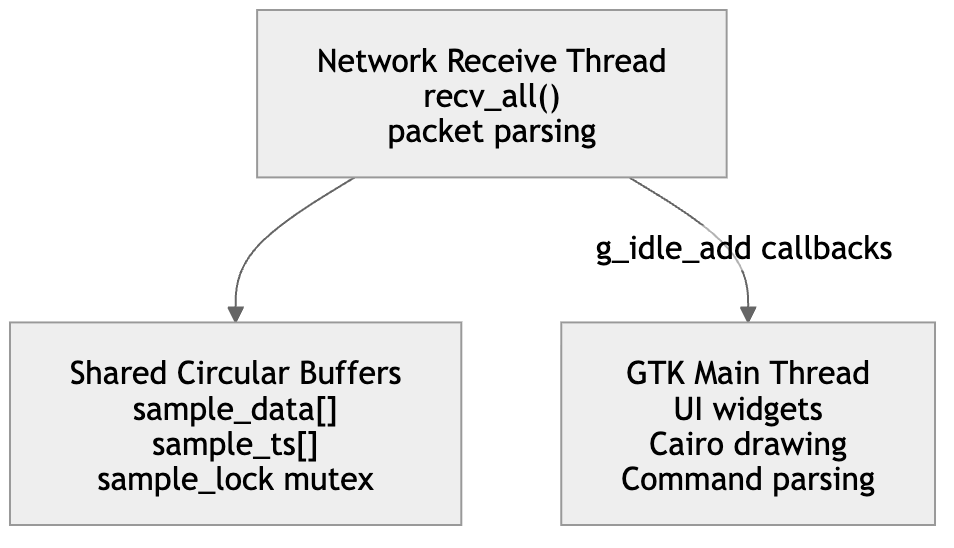
\includegraphics[scale = 0.5]{media/ameerapp9.png}
    \caption{GTK and Network Thread Separation}
    \label{fig-ameergui1}
\end{figure}

This design is reflected directly in the core synchronization primitives defined in the GUI implementation:

\begin{minted}[bgcolor = lightgray, fontsize = \footnotesize]{c}
static pthread_t net_thread;
static volatile int net_running = 0;

static pthread_mutex_t sample_lock = PTHREAD_MUTEX_INITIALIZER;
\end{minted}

The \texttt{net\_thread} executes the blocking receive loop, while the \texttt{net\_running} flag provides a lightweight, thread-safe termination mechanism used during disconnect and shutdown sequences. Shared access to sensor sample buffers is protected by \texttt{sample\_lock}, ensuring deterministic behavior when the network thread inserts new data and the GTK thread simultaneously renders plots or extracts values for display.

By isolating all network I/O inside a dedicated POSIX thread and strictly enforcing GTK-only access from the main loop, the architecture guarantees that user interactions such as window resizing, command entry, or sensor selection remain responsive regardless of network latency or streaming rate. This approach mirrors the separation of concerns used on the server side, where acquisition, communication, and scheduling responsibilities are similarly decoupled.

From a system-level perspective, the GUI therefore behaves as a reactive front-end: background threads ingest and buffer data, while the GTK main loop remains focused on deterministic rendering and user interaction.


\subsection{Socket Creation and Connection Establishment}
The connection workflow is initiated when the user provides a server IPv4 address and explicitly requests a connection through the GUI. At this point, the client creates a TCP socket using the Berkeley Sockets API and prepares it for controlled, non-blocking connection establishment. This approach ensures that the graphical interface remains responsive even when the remote server is unreachable or slow to accept connections.

To prevent the GUI from blocking during the \texttt{connect()} call, the
socket is temporarily configured in non-blocking mode. This allows the
application to initiate the connection asynchronously while retaining full
control over timeout behavior. The following excerpt illustrates the core
mechanism used during the connection phase:


\begin{minted}[bgcolor = lightgray, fontsize = \footnotesize]{c}
sock_fd = socket(AF_INET, SOCK_STREAM, 0);
fcntl(sock_fd, F_SETFL, O_NONBLOCK);

res = connect(sock_fd, (struct sockaddr *)&addr, sizeof(addr));
if (res < 0 && errno == EINPROGRESS)
{
    select(sock_fd + 1, NULL, &wfds, NULL, &timeout);
}
\end{minted}

In this configuration, \texttt{connect()} typically returns immediately with
\texttt{EINPROGRESS}, indicating that the connection attempt is still in
progress. The \texttt{select()} system call is then used to wait for the
socket to become writable within a bounded time interval. A three-second
timeout is applied to ensure deterministic behavior; if the socket does not
signal completion within this period, the connection attempt is aborted, the
socket is closed, and the user is notified via the GUI.

After \texttt{select()} returns, the connection result is verified using
\texttt{getsockopt()} with the \texttt{SO\_ERROR} option to distinguish a
successful connection from a failed attempt. Only if this check confirms
success does the GUI proceed to the next stage.

Once the connection attempt completes successfully, the socket is explicitly
restored to blocking mode. This design choice simplifies all subsequent
network operations: steady-state data reception is handled inside a dedicated
network receive thread, where blocking \texttt{recv()} calls provide
predictable control flow, reduced CPU usage, and eliminate the need for
polling or partial-read handling logic.

Immediately after restoring blocking mode, the GUI spawns the network receive
thread and transitions its internal state to indicate an active connection.
This staged strategy---non-blocking during connection establishment and
blocking during steady-state streaming---reflects common industrial client
implementations and achieves a balance between user-interface responsiveness
and reliable, low-complexity data handling.

\subsection{IPv4 Address Validation and Defensive Input Handling}
Before attempting any network operation, the GUI performs strict validation of the user-supplied IPv4 address. Instead of relying on permissive system-level parsing, the application enforces an exact dotted-decimal format consisting of four octets, each constrained to the valid range of 0 to 255.

This validation is executed locally within the GUI layer to prevent unnecessary socket creation attempts and to provide immediate, deterministic feedback to the user. Inputs containing missing octets, trailing characters, non-numeric tokens, or out-of-range values are explicitly rejected before any networking API is invoked.

The validation logic relies on strict pattern matching using sscanf(), ensuring that the input string contains exactly four numeric fields and no additional characters:
\begin{minted}[bgcolor = lightgray, fontsize = \footnotesize]{c}
if (sscanf(ip, "%d.%d.%d.%d%c", &a, &b, &c, &d, &tail) != 4)
    return FALSE;
\end{minted}

By rejecting malformed input at the earliest possible stage, the GUI avoids undefined behavior at lower networking layers and eliminates ambiguous error conditions that would otherwise surface during socket creation or connection attempts. This defensive approach improves both robustness and debuggability, particularly in failure scenarios involving invalid user input.

The outcome of the validation is immediately reflected in the graphical interface through dynamic visual feedback. The input field is styled to indicate success or error conditions, reinforcing correct usage patterns and reducing the likelihood of repeated invalid attempts. This tight integration of validation logic and UI feedback contributes to a safer and more user-friendly connection workflow.

\subsection{GUI State Machine Design}
The GUI implements an internal client-side state machine that is intentionally
distinct from the server's streaming state machine. While the server operates
using internal states such as \texttt{STREAM\_IDLE}, \texttt{STREAM\_RUNNING},
and \texttt{STREAM\_DISCONNECT} to manage data production and transmission,
the GUI maintains a higher-level, connection-oriented view of system
operation. This separation ensures that client-side logic remains focused on
user interaction, command validity, and visualization control rather than
internal server behavior.

From the GUI's perspective, system operation is fully characterized by three
states. In the disconnected state, no TCP connection exists and all
network-related actions are disabled. The connected state represents a
successfully established TCP connection in which the system is ready to accept
user commands but is not yet receiving streaming data. The running state
indicates that real-time sensor data streaming is active and being processed
and visualized by the GUI.


\begin{figure}[H]
    \centering 
    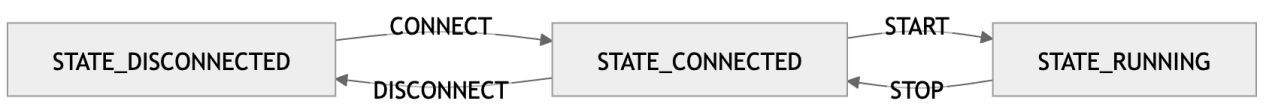
\includegraphics[scale = 0.9]{media/ameerapp10.png}
    \caption{Client Connection State Machine}
    \label{fig-ameergui2}
\end{figure}

State transitions are strictly validated before execution to prevent illegal command sequences and unsafe operations. For example, streaming can only be initiated when the GUI is already connected, and disconnection is explicitly blocked while streaming is active. The following excerpt illustrates a guarded transition from the connected state into the running state when the user issues a valid START command:

\begin{minted}[bgcolor = lightgray, fontsize = \footnotesize]{c}
if (state == STATE_CONNECTED) {
    send(sock_fd, "START\n", 6, 0);
    state = STATE_RUNNING;
}
\end{minted}
By enforcing these constraints locally, the GUI acts as a first line of defense against invalid protocol usage. This prevents malformed or out-of-sequence commands from reaching the server and ensures that the graphical controls, internal logic, and remote system remain synchronized at all times.

\subsection{Network Receive Thread and Streaming Handling}
Once streaming is initiated, the GUI spawns a dedicated network receive thread that becomes the sole entry point for incoming data from the measurement server. This thread is intentionally isolated from all GTK operations and performs blocking socket I/O, allowing the main GUI thread to remain fully responsive during high-rate data transfers.

The server transmits sensor data using a length-prefixed framing scheme. Each transmission begins with a fixed 4-byte header indicating the size of the upcoming payload, followed by a contiguous batch of binary \texttt{sensor\_data\_t }records. Since TCP is a stream-oriented protocol with no inherent message boundaries, this framing mechanism is essential to preserve packet alignment and ensure deterministic decoding on the client side.

The receive thread first blocks until the size header is fully received, converts it from network byte order, and then continues reading until the complete payload has been transferred. This logic is implemented using a helper routine that guarantees full reception before processing:
\begin{minted}[bgcolor = lightgray, fontsize = \footnotesize]{c}
recv_all(sock_fd, &net_size, sizeof(net_size));
payload_size = ntohl(net_size);
recv_all(sock_fd, batch, payload_size);
\end{minted}

To support this behavior, a blocking helper function repeatedly invokes \texttt{recv()} until the requested number of bytes has been obtained or an error occurs:

\begin{minted}[bgcolor = lightgray, fontsize = \footnotesize]{c}
static int recv_all(int fd, void *buf, size_t len)
{
    size_t off = 0;
    while (off < len)
    {
        ssize_t n = recv(fd, (char *)buf + off, len - off, 0);
        if (n <= 0)
            return -1;
        off += n;
    }
    return 0;
}
\end{minted}

This approach eliminates partial-read corner cases and ensures that each batch is processed atomically. Once the payload has been successfully received, the thread iterates through the decoded sensor records and forwards them to the circular buffer layer via the \texttt{push\_sample()} interface.

\begin{figure}[H]
    \centering 
    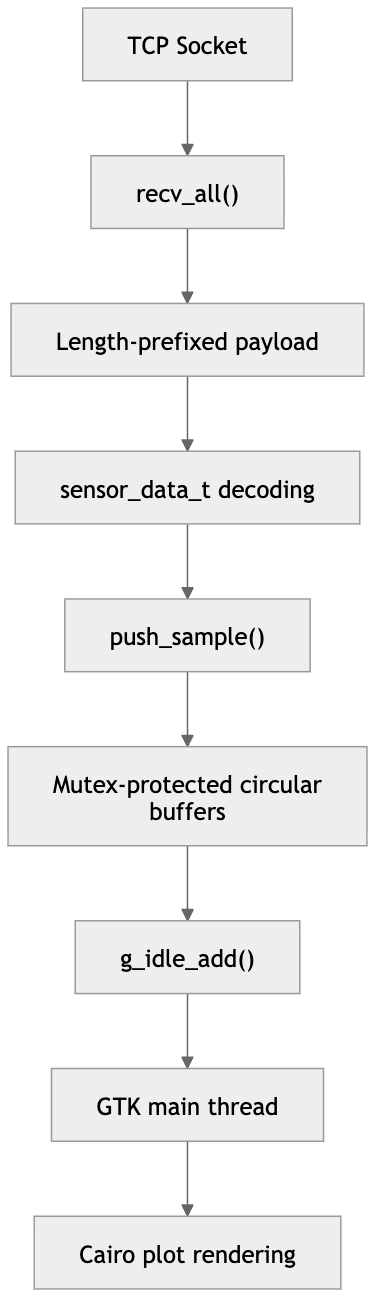
\includegraphics[scale = 0.7]{media/ameerapp2.png}
    \caption{Client-Side Data Flow Pipeline}
    \label{fig-ameergui2}
\end{figure}

Crucially, the receive thread never updates GUI elements directly. Instead, it schedules redraw operations and auxiliary UI updates using \texttt{g\_idle\_add()}, which defers execution to the GTK main loop. This design strictly adheres to GTK’s thread-safety model and prevents undefined behavior caused by cross-thread widget access.
 
In the event of a socket error, malformed payload, or remote disconnect, the receive loop terminates gracefully. The thread then signals the main thread to reset the plotting state, close the socket, and transition the GUI back into a disconnected state. This controlled shutdown sequence ensures that resources are released safely and that the application never remains in an inconsistent or partially connected condition.

\subsection{Circular Buffer Handling and Sample Insertion}
Incoming sensor samples received by the network thread are stored in fixed-size circular buffers, one buffer per sensor. Each buffer maintains its own head index and sample counter, allowing the GUI to retain only the most recent data while guaranteeing bounded memory usage regardless of streaming duration.

All write access to the buffers is protected by a POSIX mutex (sample\_lock). This ensures that concurrent access from the network receive thread and the GTK rendering logic does not result in race conditions or inconsistent state.

The core insertion mechanism follows a deterministic overwrite model. Each new sample is written at the current head position, after which the head index is advanced with wraparound logic:
\begin{minted}[bgcolor = lightgray, fontsize = \footnotesize]{c}
pthread_mutex_lock(&sample_lock);

sample_data[sid][head] = value;
sample_ts[sid][head]   = rel_ts;

sample_head[sid] = (head + 1) % MAX_SAMPLES;

if (sample_count[sid] < MAX_SAMPLES)
    sample_count[sid]++;

pthread_mutex_unlock(&sample_lock);
\end{minted}

This approach ensures that once the buffer reaches capacity, older samples are automatically overwritten by newer ones in a predictable manner. No dynamic memory allocation occurs during steady-state operation, which is essential for maintaining consistent performance under high-frequency data acquisition.

A key design element is timestamp normalization. The GUI establishes a reference timestamp (server\_t0) when the first sample is received. All subsequent timestamps are stored as offsets relative to this reference:


\begin{minted}[bgcolor = lightgray, fontsize = \footnotesize]{c}
if (server_t0 == 0)
    server_t0 = ts;

uint64_t rel_ts = ts - server_t0;
\end{minted}

This normalization simplifies later visualization and axis scaling by eliminating large absolute timestamp values and ensuring that all plotted data shares a common temporal origin. It also allows the GUI to reset its time base cleanly whenever a new connection or streaming session begins.

The circular buffers therefore serve as a stable synchronization boundary between asynchronous data ingestion and deterministic GUI rendering, enabling smooth real-time visualization without unbounded memory growth.

\subsection{GUI–Network Interaction Model}
Direct interaction between background threads and GTK widgets is strictly prohibited in the application design. GTK enforces a single-threaded UI model in which all widget updates, rendering operations, and state changes must occur within the main GTK thread. Violating this rule can lead to race conditions, segmentation faults, or undefined rendering behavior. As a result, the GUI–network interaction is implemented using a strictly event-driven synchronization mechanism.

The network receive thread is therefore designed to operate in complete isolation from the GUI layer. Its responsibilities are limited to blocking socket I/O, decoding incoming protocol messages, and inserting validated sensor samples into mutex-protected circular buffers. At no point does this thread directly invoke GTK drawing routines or manipulate widget state.

To bridge the gap between background processing and UI updates, the GUI leverages GTK’s idle event mechanism. Whenever new data arrives or a state transition must be reflected visually, the network thread schedules a deferred callback using \texttt{g\_idle\_add()}. This registers a lightweight task that is executed asynchronously by the GTK main loop when it reaches an idle state.

\begin{minted}[bgcolor = lightgray, fontsize = \footnotesize]{c}
g_idle_add((GSourceFunc)gtk_widget_queue_draw, graph_area);
\end{minted}

This approach guarantees that all rendering activity, including plot redraws and widget refreshes, is executed safely within the GTK thread context. The same mechanism is reused for non-graphical updates, such as appending entries to the live sensor information panel or updating connection status labels following network events.

By enforcing a unidirectional interaction model—where background threads publish events and the GUI consumes them—the implementation achieves strong temporal decoupling between data acquisition and visualization. This design not only preserves thread safety but also ensures that GUI responsiveness is unaffected by network latency, bursty data arrival, or temporary connection instability.

The event-driven interaction model thus forms a critical stability boundary within the client architecture. It allows high-frequency sensor streaming to coexist with a responsive graphical interface, while maintaining strict compliance with GTK’s threading constraints.

\subsection{GUI Utility Layer}
The GUI utility layer provides a compact collection of shared helper functions and data structures that support the main GUI logic without embedding auxiliary concerns directly into gui.c. Its primary role is to centralize functionality that is reused across multiple GUI subsystems, thereby improving code clarity, maintainability, and separation of concerns.

At the functional level, the utility layer encapsulates three main responsibilities: defensive input validation, lightweight widget state management, and consistent visual feedback through runtime CSS injection. By isolating these tasks, the core GUI implementation remains focused on application logic, networking, and visualization rather than low-level UI mechanics.

A key example is IPv4 address validation, which is implemented once in the utility layer and reused by both button-driven and CLI-driven connection workflows. This avoids duplicated validation logic and ensures consistent behavior regardless of how a connection is initiated.
\begin{minted}[bgcolor = lightgray, fontsize = \footnotesize]{c}
gboolean is_valid_ipv4(const char *ip)
{
    int a, b, c, d;
    char tail;
    if (sscanf(ip, "%d.%d.%d.%d%c", &a, &b, &c, &d, &tail) != 4)
        return FALSE;
    return (a >= 0 && a <= 255 &&
            b >= 0 && b <= 255 &&
            c >= 0 && c <= 255 &&
            d >= 0 && d <= 255);
}
\end{minted}

In addition to validation helpers, the utility layer defines the shared data structures that form the binary protocol contract between the GUI client and the server. These structures are intentionally placed in \texttt{utils.h} to guarantee that both networking code and visualization logic operate on a common, unambiguous data model.

\begin{minted}[bgcolor = lightgray, fontsize = \footnotesize]{c}
typedef struct
{
    sensor_id_t sensor_id;
    unsigned int sensor_value;
    uint64_t timestamp;
} sensor_data_t;

typedef struct
{
    sensor_rate_t rates[SENSOR_COUNT];
} RatesMsg;
\end{minted}

The \texttt{sensor\_data\_t} structure represents a single atomic sensor sample transmitted by the server, while RatesMsg encapsulates the sampling configuration exchanged at the start of streaming. Together, these definitions ensure binary compatibility between the server’s transmit logic and the GUI’s receive and decode paths, reducing the risk of protocol mismatches.
Finally, the utility layer manages GUI-specific presentation details such as command feedback styling. Custom CSS rules are injected at runtime to visually distinguish successful commands, invalid input, and focus transitions, without hard-coding presentation logic into widget callbacks.

\begin{minted}[bgcolor = lightgray, fontsize = \footnotesize]{c}
gtk_css_provider_load_from_data(provider,
    "entry.cmd-success { border: 2px solid #2ecc71; }"
    "entry.cmd-error   { border: 2px solid #e74c3c; }",
    -1, NULL);
\end{minted}

By confining these responsibilities to a dedicated utility module, the GUI implementation achieves a cleaner architectural structure. The result is a client application that is easier to extend, debug, and reason about, while preserving a clear boundary between core behavior and supporting infrastructure.

\subsection{Summary and Observations}
The GUI client implementation provides a stable and efficient front-end for interacting with the Measurement Network Gateway under real-time operating conditions. By separating graphical operations from network communication and enforcing strict execution boundaries between threads, the design maintains responsiveness even during high-frequency data streaming.

A dedicated network receive thread, combined with mutex-protected circular buffers and GTK’s idle-event scheduling, ensures safe and deterministic data flow from the TCP socket to the visualization layer. Defensive IPv4 validation and a clearly defined client-side state machine prevent invalid command sequences and maintain consistency between user actions, GUI controls, and server behavior.

Overall, the GUI complements the server architecture by offering a scalable, robust, and user-oriented interface for real-time measurement monitoring, while adhering to sound systems programming practices suitable for high-throughput embedded and networked applications.




\clearpage 
\null 
\vfill 
\begin{center}
\textbf{\large Haizon Helet Cruz (42708)}
\end{center}
\vfill 
\fancyhead[L]{MNG GUI (Haizon Helet Cruz 42708)}
\clearpage


\chapter{MNG GUI Part II}
\section{GUI PLOTTING}
This section handles the plotting of the graph for individual sensors which are sent from the network thread. This is a framed drawing area for live plotting using \texttt{gtk\_frame\_new}, which creates a \texttt{GtkFrame} container and the string ``Plot'' becomes the visible title of the frame. The section is set to expand the window vertically when the window resizes.

The drawing area is created using \texttt{gtk\_drawing\_area\_new} which renders a blank canvas and the graph is drawn using the Cairo library. The canvas is supposed to occupy the whole of section B, even in cases where the window resizes. Then this plot is connected to corresponding functions \texttt{draw\_grid}, \texttt{gtk\_widget\_queue\_draw}, \texttt{update\_info\_text\_colors}, which are used to render the graph. This section also includes the text box which displays the last 10 values of temperature and ADC.

\subsection{DATA FLOW}
Incoming sensor information is organized into a dedicated circular buffer managed by the \texttt{push\_sample()} function. Each individual sensor maintains a structured dataset consisting of \texttt{id}, \texttt{value} and \texttt{timestamp} defined as a struct named \texttt{sensor\_data\_t}. These buffers are designed to accommodate required data for the purpose of plotting. To maintain integrity and prevent data collisions during concurrent operations, a synchronization mechanism utilizes mutex. This lock regulates all access to the shared sample buffers, ensuring that the ingestion of new packets occurs in a thread-safe manner. By acquiring this mutex before any modification to the circular arrays, the system prevents race conditions and guarantees that the internal state of the sensor data remains consistent and reliable for any process attempting to read or write to the memory.

The architecture maintains a clean separation between data ingestion and the user interface to ensure overall stability. Background processes are prohibited from directly modifying graphical elements instead the \texttt{g\_idle\_add} is used to schedule necessary updates. This approach delegates all rendering tasks to the GTK main thread, ensuring that the GUI remains responsive and that all visual modifications are executed within the correct execution context.

The visualization employs a dynamic windowing strategy to ensure that only the most relevant sensor data is rendered on screen. By identifying the most recent timestamp across all active sensors denoted as \texttt{t\_max}, the GUI plot establishes a temporal anchor for the display. A lower boundary \texttt{t\_min}, is then calculated using the formula \texttt{t\_min = t\_max - time\_window\_us}. During the rendering phase, any samples with timestamps failing outside this range are clipped, ensuring the graph remains focused on the current activity and prevents visual clutter from stable data. The duration of this visible window, defined by \texttt{time\_window\_us}, is not static but scales intelligently based on the incoming sampling frequency. This is particularly critical for high rate sources like ADC0, where the window must balance detail with performance.

\subsection{COORDINATE TRANSFORMATION AND SIGNAL NORMALIZATION}
Once the visible time interval is determined through the dynamic windowing
mechanism, each valid sample must be transformed from data-space into
screen-space coordinates. This conversion is performed during the rendering
phase inside the Cairo draw callback. The horizontal coordinate is calculated
by linearly mapping each timestamp within the interval $[t_{min}, t_{max}]$
to the available plotting width. This ensures that the leftmost edge of the
graph corresponds to the beginning of the visible time window, while the
rightmost edge reflects the most recent data sample.

The vertical coordinate is computed using a normalization strategy that allows
multiple sensors to be plotted simultaneously on a unified scale, Since
different sensors operate over different numeric ranges, each sensor is
associated with a defined maximum range in the array
\texttt{sensor\_y\_\_max}. During rendering, raw values are divided by their
respective maximums to obtain a normalized ratio between 0 and 1. This ratio
is then scaled to the height of the plotting region. Clamping is applied where
necessary to prevent graphical overflow. This approach simplifies comparative
visualization and maintains consistent scaling across multiple sensor types
without requiring dynamic axis configuration.

\subsection{GRID, AXES and TICK CONSTRUCTION}
To improve interpretability, the plotting system renders a structured
background consisting of grid lines, axes, tick marks and axis labels. The
grid is drawn first using faint, semi-transparent lines to provide spatial
reference without overpowering the sensor traces. Vertical grid lines
correspond to grid progression, while horizontal grid lines represent
normalized value increments. The axes are rendered with greater line thickness
to distinguish them from the grid. Directional arrows are added to both axes
to indicate increasing time and increasing signal magnitude. Tick marks are
placed at uniform pixel intervals, and corresponding numeric labels are
computed dynamically. For the X-axis, timestamps are converted to milliseconds
and formatted to avoid excessive digit length, reducing visual clutter, The
Y-axis labels reflect normalized values within the $0$--$1$ range. Axis titles
are rendered with appropriate font scaling and positioning. THe Y-axis title
is rotated vertically using the Cairo transformation matrix, ensuring
conventional scientific plot orientation.

\subsection{MULTI-SENSOR RENDERING AND TRACE STYLING}
The plotting subsystem supports simultaneous visualization of up to two
sensors. This constraint is enforced at the user interface level to maintain
clarity and prevent excessive graphical overlap. During each redraw cycle, the
renderer iterates through the selected sensors and extracts only the samples
that fell within the active window.

For each sensor, a continuous line trace is drawn by sequentially connecting
visible samples. Cairo path operations are used to move to the first valid
coordinate and then draw line segments to subsequent points. Each sensor trace
is assigned a distinct color selected from a predefined palette to ensure
clear differentiation. Line thickness is increased slightly relative to the
grid lines to enhance visibility. By decoupling the rendering logic from the
packet arrival rate and instead relying on periodic redraw scheduling, the
system ensures that trace updates remain smooth and consistent even under
high-frequency sampling conditions.


\subsection{DYNAMIC LEGEND RENDERING AND THEME ADAPTION}
To aid interpretation, a dynamic legend is rendered directly within the
plotting area. The legend displays only the currently selected sensors and
includes a colored marker alongside each sensor label. The dimensions of the
legend box are computed at runtime based on the width of the text elements,
ensuring that the container adapts automatically to varying content. The
legend background color is not statically defined. Instead, the GUI retrieves
the active GTK theme colors and performs luminance analysis to adjust the
legend background for sufficient contrast. In darker themes, the background is
slightly lightened while in lighter themes it is subtly darkened. This
guarantees readability regardless of the user's selected interface theme.
Additionally, style update signals trigger automatic redraws when the GTK
theme changes, maintaining visual consistency.

\begin{figure}[H]
\centering 
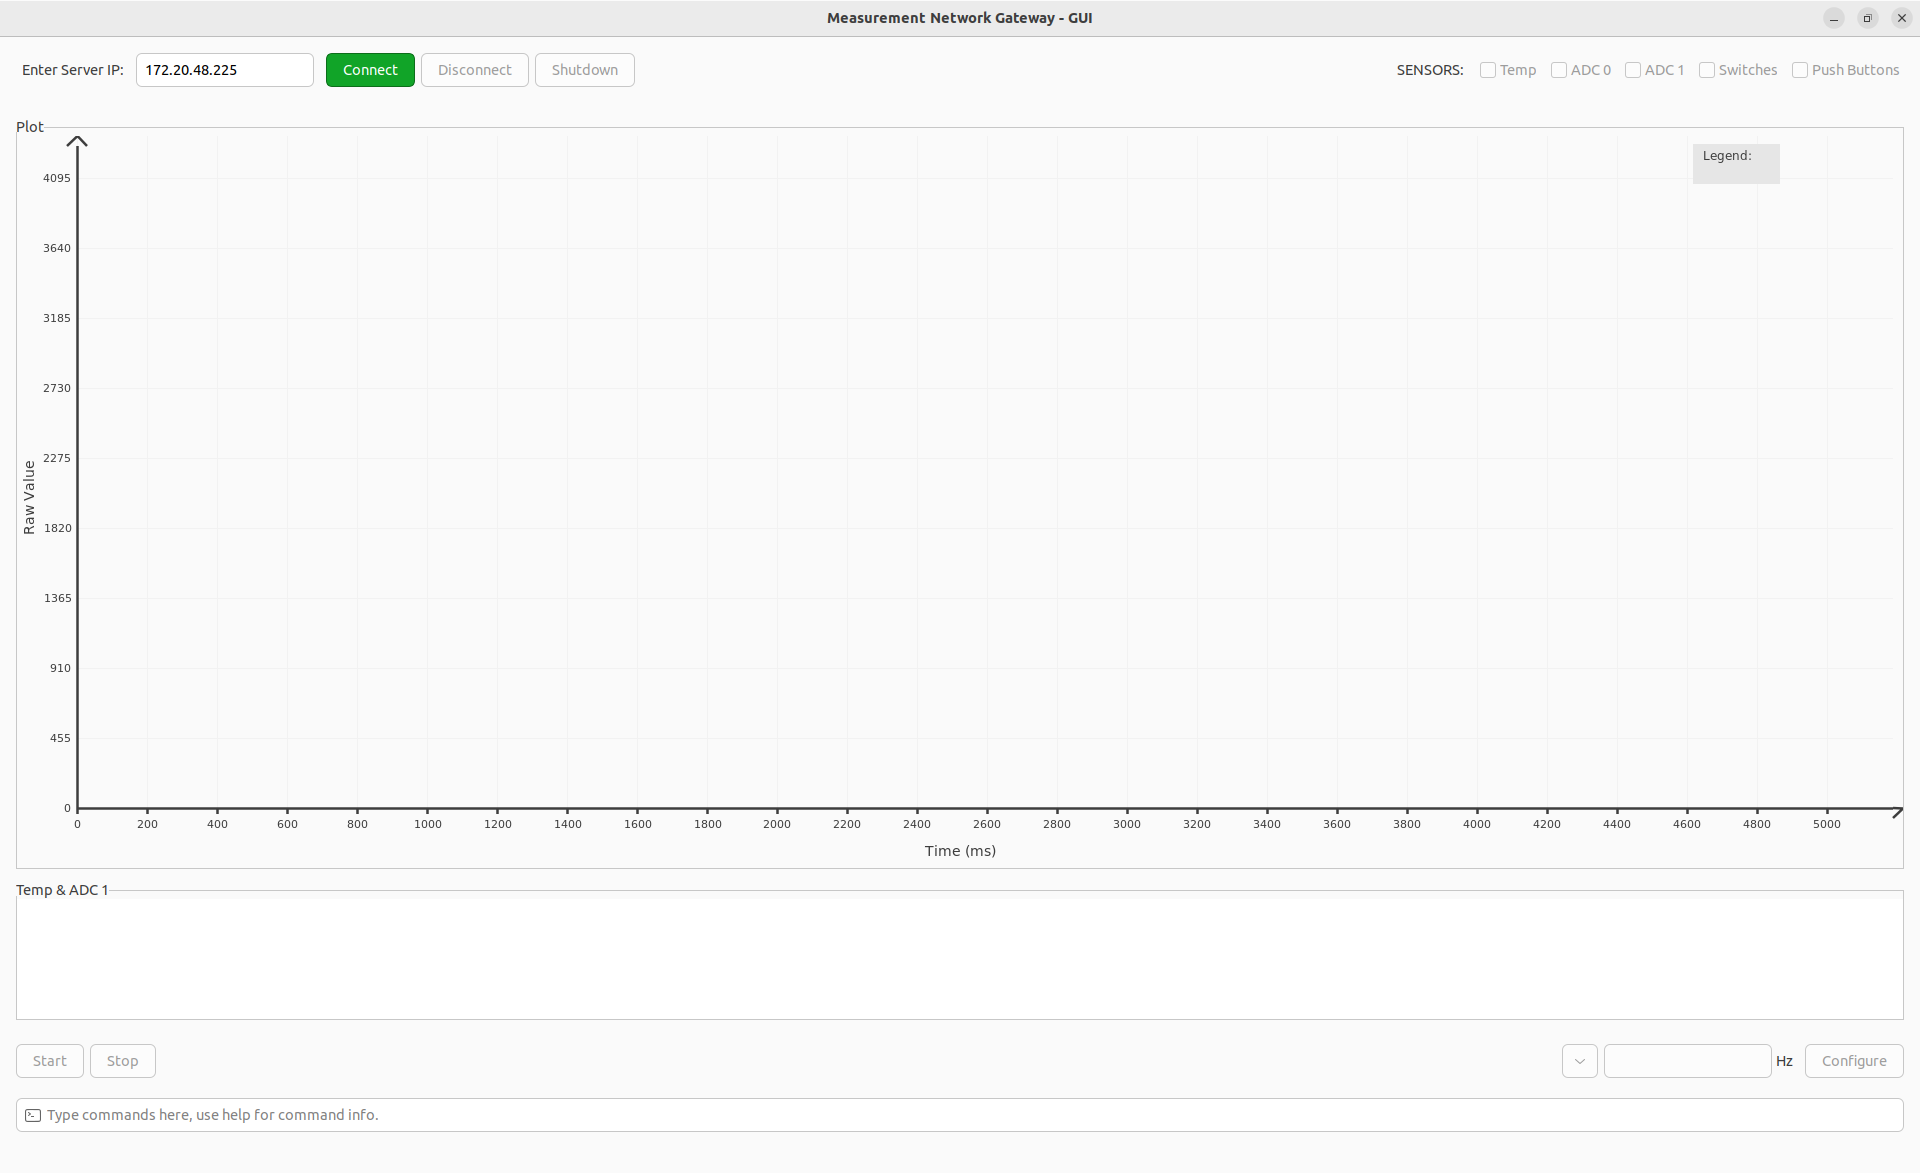
\includegraphics[width = \textwidth]{media/guihaa5.png}
\label{fig-guihaa5}
\end{figure}

\begin{figure}[H]
\centering 
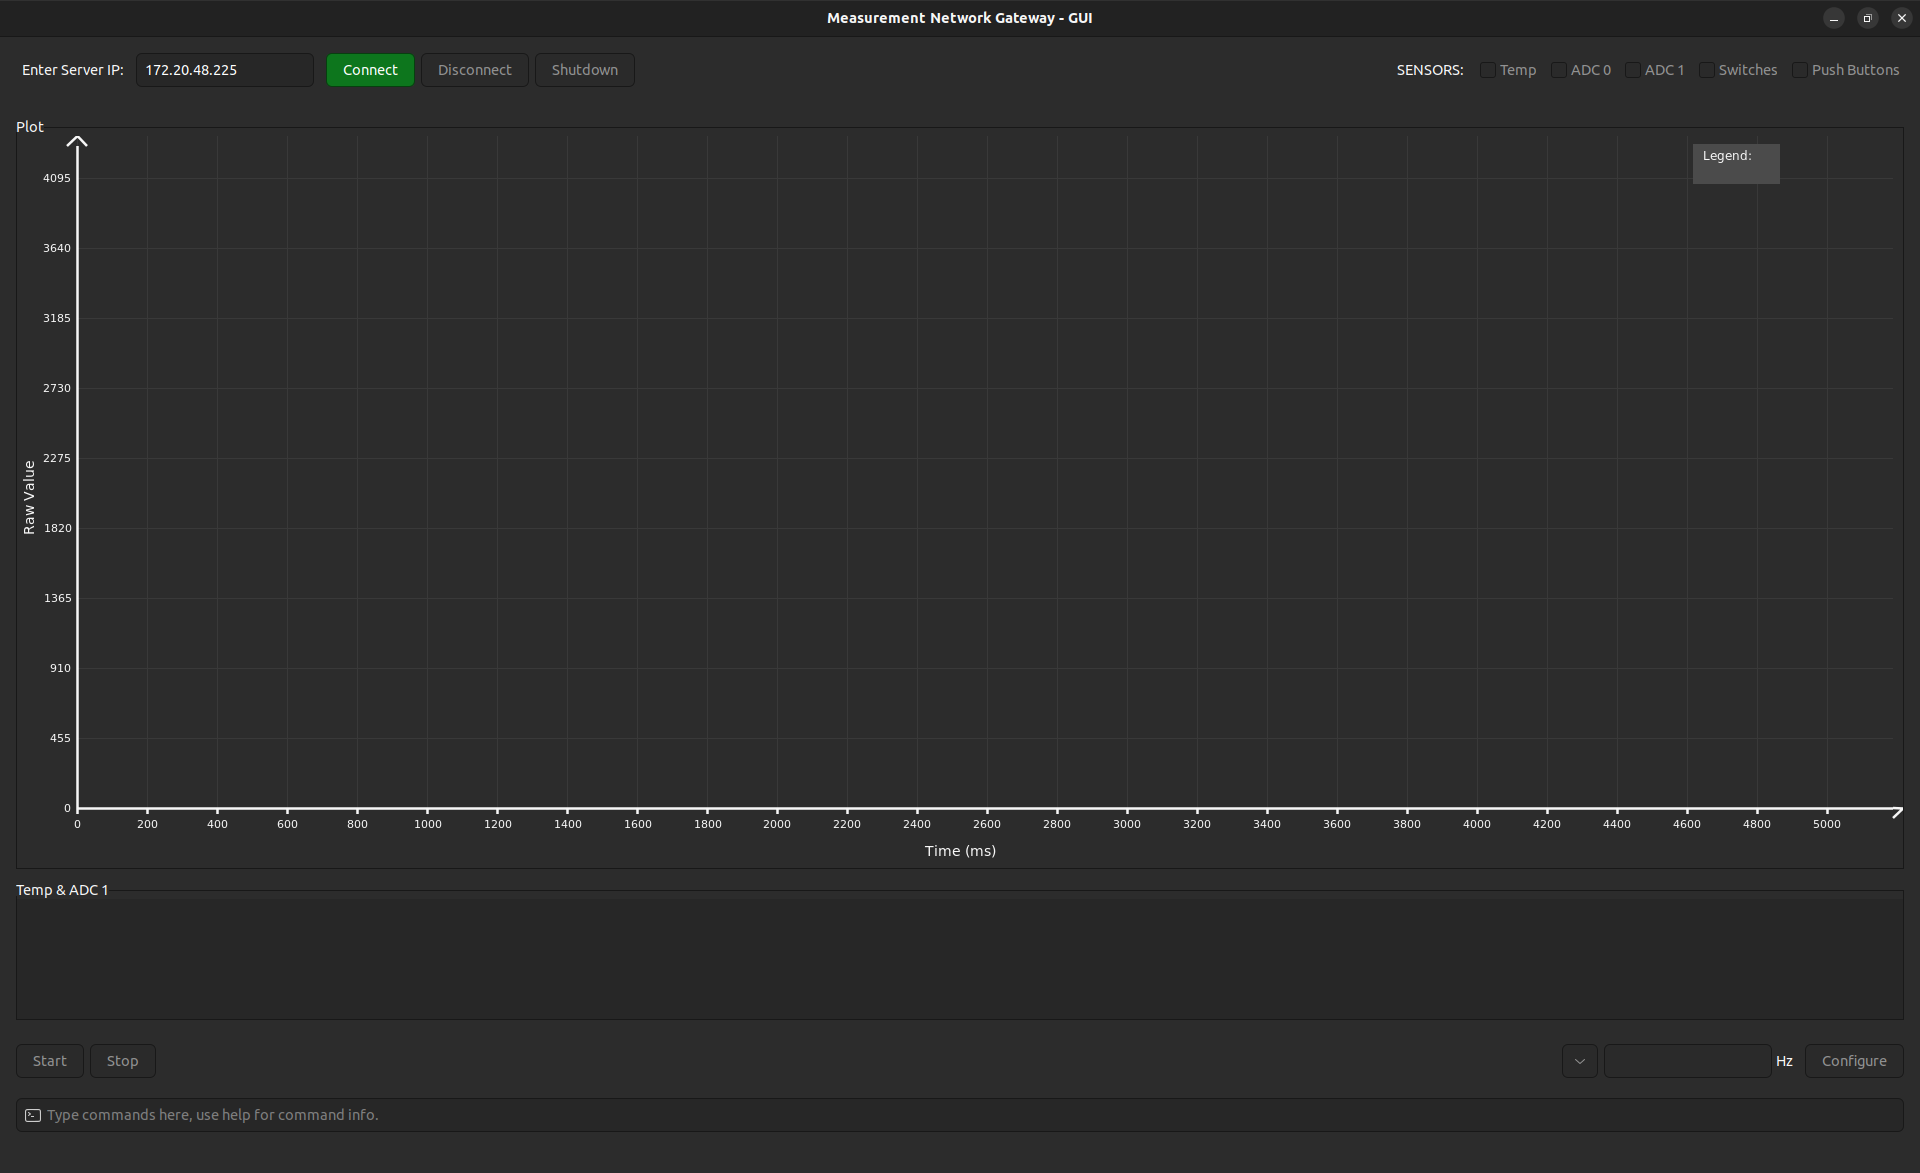
\includegraphics[width = \textwidth]{media/guihaa6.png}
\label{fig-guihaa6}
\end{figure}

\clearpage 
\section{Redraw Strategy and Performance Consideration}
Rather than redrawing the plot upon every incoming sample, the application
employs a timed refresh mechanism using a 33-millisecond interval. This
corresponds to approximately 30 frames per second, which provides visually
smooth updates while limiting unnecessary computational load. The use of
circular buffers further enhances performance by preventing unbounded memory
growth and eliminating the need for dynamic memory allocation during plotting
operation. This design ensures that rendering workload remains predictable and
stable even when sensors operate at higher sampling frequencies. By separating
data acquisition, buffering, and visualization into distinct functional layers,
the architecture maintains responsiveness and scalability.

\begin{figure}[H]
\centering 
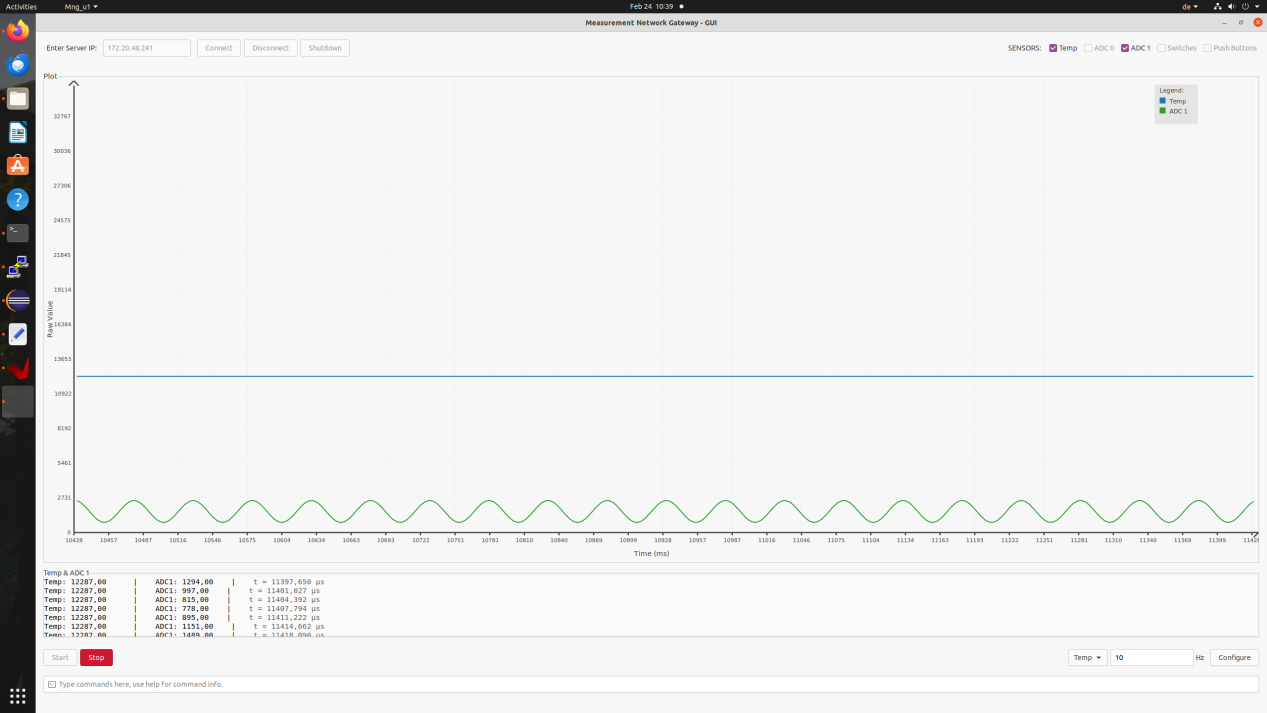
\includegraphics[width = \textwidth]{media/guihaa7.png}
\label{fig-guihaa7}
\end{figure}

\begin{figure}[H]
\centering 
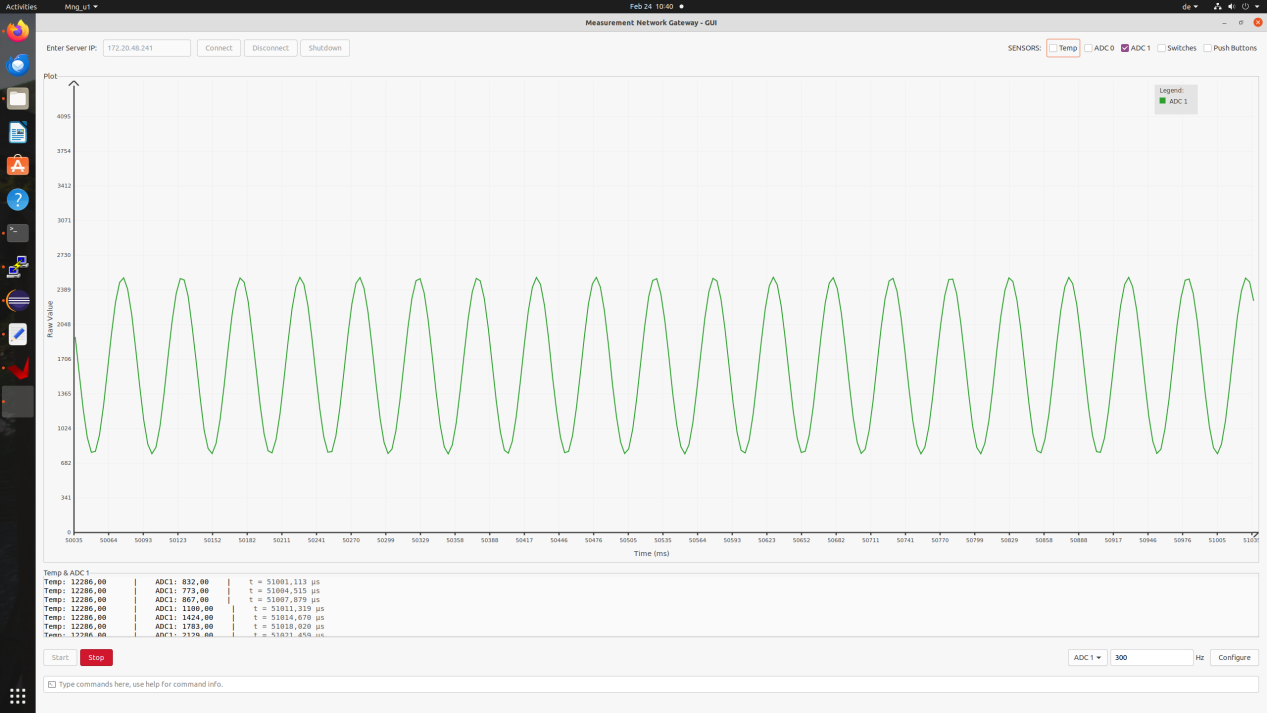
\includegraphics[width = \textwidth]{media/guihaa8.png}
\label{fig-guihaa8}
\end{figure}

\section{Live Sensor Information Panel}
Complementing the graphical plot, the interface includes a textual information
panel positioned below the main drawing area. This component displays the ten
most recent temperature and ADC1 measurements along with their corresponding
timestamps. The monospace font preserves column alignment. Whenever a new ADC1
sample is received, a formatted entry containing temperature, converted ADC
voltage, and relative timestamp is appended to the buffer. If the number of
lines exceeds 10, the oldest entry is automatically removed to maintain a
fixed-length history. Text tags are used to apply consistent color styling to
different data fields, enhancing readability. This panel serves as a numerical
complement to the graphical representation, allowing users to inspect precise
values while simultaneously observing real-time trends in the plot.

\begin{figure}[H]
\centering 
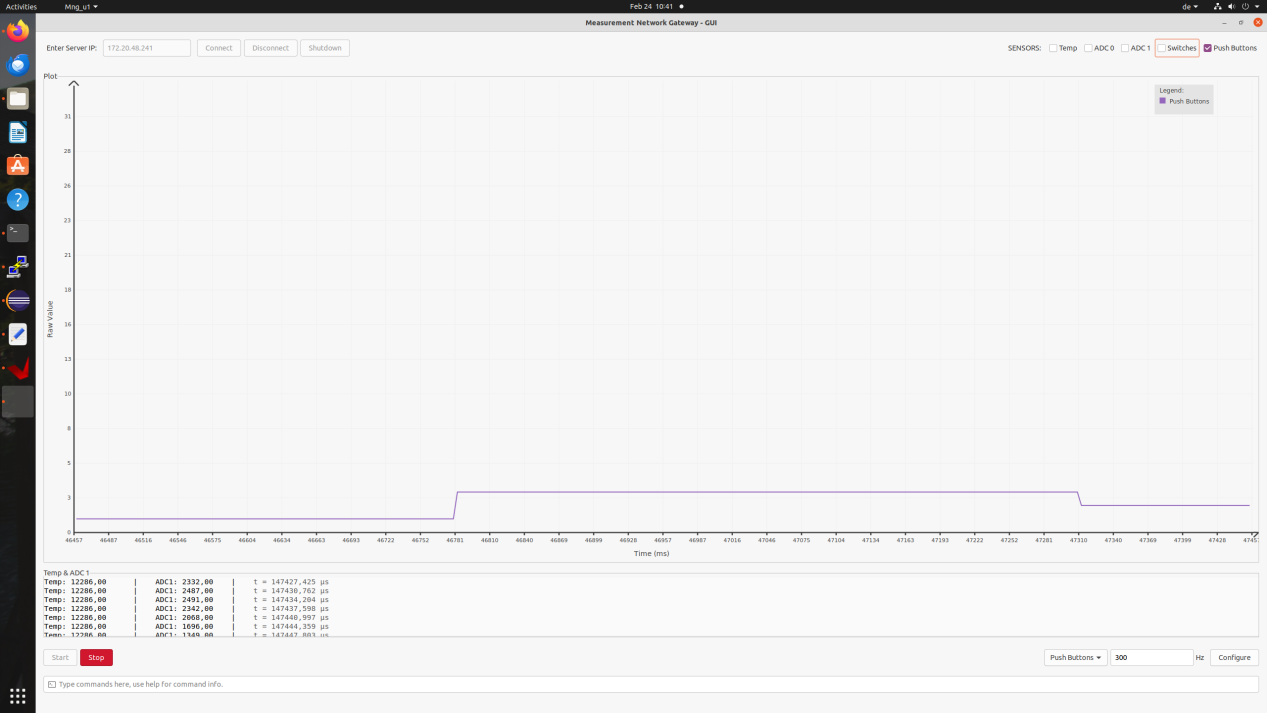
\includegraphics[width = \textwidth]{media/guihaa9.png}
\label{fig-guihaa9}
\end{figure}

\section{Command Line Interface}
The application includes an integrated command-line interface (CLI) help system
that provides structured guidance for all supported textual commands. When the
user enters the \texttt{HELP} command, a dedicated terminal window is launched
displaying a formatted reference guide. This help interface clearly categorizes
valid commands, usage syntax, parameter requirements, example invocations,
invalid usage scenarios, and operational constraints. The terminal output uses
visual formatting to distinguish command keywords, examples, warnings, and
notes, thereby improving readability and reducing user error.

The CLI supports core operational commands including \texttt{CONNECT},
\texttt{DISCONNECT}, \texttt{START}, \texttt{STOP}, \texttt{SHUTDOWN}, and
\texttt{CONFIGURE}. The \texttt{CONNECT <IP\_ADDRESS>} command establishes a
TCP connection to a remote measurement server, requiring a valid IPv4 address
in strict dotted-decimal format. The \texttt{DISCONNECT} command safely closes
an active connection but enforces a precondition that data streaming must be
stopped. The \texttt{START} command initiates sensor data streaming and
real-time plotting, and is valid only when a connection is active. Conversely,
the \texttt{STOP} command halts streaming and plotting and is permitted only
while the system is in a running state. The \texttt{SHUTDOWN} command instructs
the remote device to terminate operation and closes the application, provided
that streaming is not currently active.

The \texttt{CONFIGURE <SENSOR\_ID> <FREQ\_HZ>} command allows runtime
adjustment of individual sensor sampling frequencies. Supported sensor
identifiers include \texttt{TEMP}, \texttt{ADC0}, \texttt{ADC1}, \texttt{SW},
and \texttt{PB}. The frequency parameter must be an integer between 10~Hz and
1000~Hz. The help documentation explicitly provides both valid and invalid
configuration examples to clarify boundary conditions, such as rejecting
frequencies outside the permitted range. Additionally, the system enforces
logical constraints including prevention of connection attempts while already
connected, disallowing disconnection during active plotting, and requiring an
active streaming state before configuration changes are applied.

The CLI is case-sensitive and incorporates structured error feedback within the
GUI. Invalid commands or state violations trigger descriptive status messages,
ensuring that users are informed of improper usage. By combining explicit
syntax validation, state-aware command enforcement, and comprehensive help
documentation, the CLI subsystem enhances usability while maintaining
operational safety and system integrity.

\begin{figure}[H]
\centering 
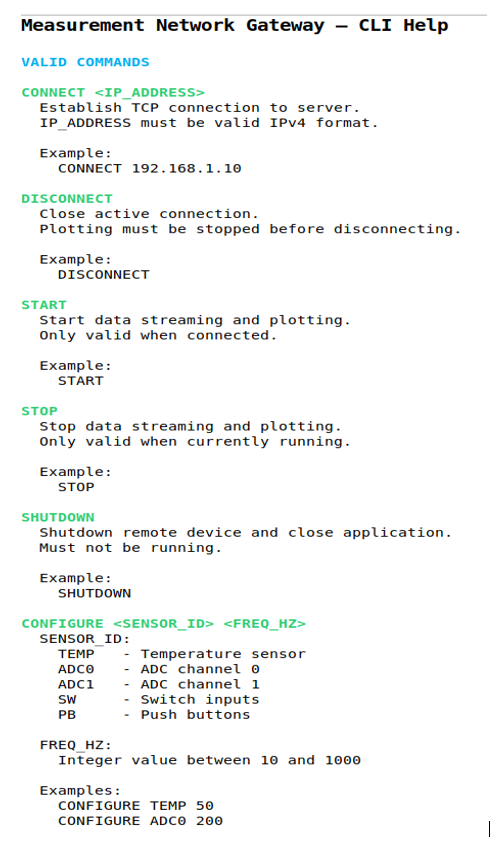
\includegraphics[width = 0.6\textwidth]{media/guihaa10.png}
\label{fig-guihaa10}
\end{figure}

\begin{figure}[H]
\centering 
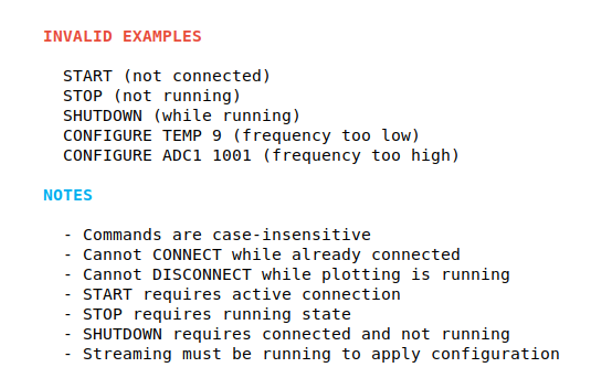
\includegraphics[width = 0.8\textwidth]{media/guihaa11.png}
\label{fig-guihaa11}
\end{figure}

\subsection{SUMMARY}
The plotting subsystem integrates asynchronous data acquisition, synchronized
buffering, and deterministic rendering into a cohesive real-time visualization
framework. Incoming sensor packets are received in a dedicated thread and
inserted into protected circular buffers, ensuring bounded memory usage and
deterministic overwrite behavior. Mutual exclusion guarantees data integrity
during concurrent access, while \texttt{g\_idle\_add} enforces strict
separation between background processing and GTK's main-thread rendering
context. Visualization is performed through a Cairo-based drawing pipeline
within a \texttt{GtkDrawingArea}, refreshed at a controlled interval of
approximately 30 frames per second. A sliding time-window mechanism ensures
that only the most recent and relevant data is displayed, providing a
continuously scrolling view of sensor activity. Samples are normalized to a
unified vertical scale, allowing multiple sensor types to be plotted
simultaneously without dynamic axis reconfiguration. The GUI plot subsystem
further enhances usability through structured grid rendering, dynamic axis
labeling, color-coded multiple sensor traces, and a theme-aware legend. An
auxiliary numerical panel complements the graphical plot by presenting the
latest temperature and ADC values in a bounded textual log. Altogether, the
architecture balances responsiveness, performance stability and clarity of
presentation, resulting in a robust and scalable real-time monitoring
interface.



\clearpage 
\null 
\vfill 
\begin{center}
\textbf{\large Alin Raj Rajagopalan Nair (41520)}
\end{center}
\vfill 
\fancyhead[L]{MNG GUI (Alin Raj Rajagopalan Nair 41520)}
\clearpage


\chapter{MNG GUI Part III}
\section{GUI} 

\subsection{Command Handling}
\begin{enumerate}
    \item \textbf{CONNECT Command}

    Syntax: \texttt{CONNECT <IP\_ADDRESS>}

    \begin{enumerate}
        \item Establishes TCP/IP connection to the remote measurement server on port 50012 using the specified IPv4 address
        \item Implements non-blocking socket creation with 3-second timeout to prevent GUI freezing during connection attempts
        \item Upon successful connection, automatically spawns a dedicated pthread for asynchronous network data reception
        \item Transitions application state from DISCONNECTED to CONNECTED and pre-selects Temperature and ADC1 sensors for immediate visualization
        \item Example: \texttt{CONNECT 192.168.1.10}
    \end{enumerate}

    \item \textbf{DISCONNECT Command}

    Syntax: \texttt{DISCONNECT}

    \begin{itemize}
        \item Gracefully terminates the active TCP connection and stops the network receive thread using \texttt{pthread\_join()} for safe cleanup
        \item Can only be executed when in CONNECTED state; returns error if attempted while streaming is active (must STOP first)
        \item Closes socket file descriptor, clears all sensor circular buffers, and resets timestamp synchronization reference (\texttt{server\_t0})
        \item Transitions application state back to DISCONNECTED, re-enabling the IP entry field and Connect button
        \item Example: \texttt{DISCONNECT}
        \item Error Example: \texttt{DISCONNECT} \\
        \(\rightarrow\) Error: ``Cannot disconnect: GUI is running, stop and disconnect.'' \\
        (when attempted during RUNNING state)
    \end{itemize}

    \item \textbf{START Command}

    Syntax: \texttt{START}

    \begin{itemize}
        \item Sends ASCII \texttt{"START\textbackslash n"} command to the server, initiating real-time binary sensor data streaming over the established TCP connection
        \item Enables sensor selection checkboxes with 2-sensor maximum constraint and activates frequency configuration controls
        \item Transitions state from CONNECTED to RUNNING; disables Disconnect and Shutdown buttons to prevent unsafe operations during streaming
        \item Server responds with initial RATES configuration message followed by continuous batches of \texttt{sensor\_data\_t} structures
        \item Example: \texttt{START}
        \item Typical Workflow Example:
        \begin{enumerate}
            \item \texttt{CONNECT 192.168.1.10}
            \item \texttt{START}
            \item (Data streaming begins, graph updates in real-time)
        \end{enumerate}
    \end{itemize}


    \item \textbf{STOP Command}

    Syntax: \texttt{STOP}

    \begin{itemize}
        \item Sends ASCII \texttt{"STOP\textbackslash n"} command to halt sensor data streaming while maintaining the TCP connection for future operations
        \item Preserves all captured data in circular buffers allowing graph inspection after streaming stops; data persists until disconnect or reconnect
        \item Transitions state from RUNNING to CONNECTED, re-enabling Disconnect and Shutdown buttons while disabling sensor configuration controls
        \item Does not terminate the network receive thread; connection remains active and ready to resume streaming with subsequent START command
        \item Example: \texttt{STOP}
        \item Typical Workflow Example:
        \begin{enumerate}
            \item \texttt{START}
            \item (Observe data for analysis)
            \item \texttt{STOP}
            \item (Graph frozen, data preserved for inspection)
            \item \texttt{START} (can restart streaming)
        \end{enumerate}
    \end{itemize}

    \item \textbf{SHUTDOWN Command}

    Syntax: \texttt{SHUTDOWN}

    \begin{itemize}
        \item Displays modal confirmation dialog before sending \texttt{"SHUTDOWN\textbackslash n"} to the remote embedded device (\texttt{/dev/meascdd}), then exits the application
        \item Automatically sends STOP command first if streaming is active, ensuring clean server-side termination before shutdown
        \item Performs complete cleanup: stops network thread with \texttt{pthread\_join()}, closes socket, clears plot state, and calls \texttt{gtk\_main\_quit()}
        \item Can only be executed from CONNECTED state (not RUNNING); prevents accidental shutdown during active data acquisition
        \item Example: \texttt{SHUTDOWN} \\
        \(\rightarrow\) Dialog: ``Are you sure you want to shutdown the device \texttt{/dev/meascdd}?'' \\
        \(\rightarrow\) User clicks ``Yes'' \(\rightarrow\) Device shuts down, application exits
    \end{itemize}

\end{enumerate}

\textbf{Command Explaination (Detailed)}
\begin{enumerate}
\item The client will send ASCII text commands through the TCP socket connection, which are parsed and executed by the GUI application. Most client commands will be processed based on the command keyword, though some may require additional parameters.
\item Before processing any command, the application will first validate the command syntax and current application state. Only if the command is valid and the state permits execution will it proceed further.
\end{enumerate}

Here are the different commands a client may send:

\begin{enumerate}
    \item \texttt{START} -- Requests data streaming from server.
    \item \texttt{STOP} -- Requests to stop data streaming.
    \item \texttt{CONFIGURE} -- Requests to change a sensor's sampling frequency.
    \item \texttt{DISCONNECT} -- Requests to disconnect from server.
    \item \texttt{SHUTDOWN} -- Requests to shut down the remote device.
    \item \texttt{CONNECT} -- Requests to establish connection with server.
\end{enumerate}

\begin{itemize}
    \item Among these, three commands (\texttt{CONNECT}, \texttt{DISCONNECT},
    \texttt{SHUTDOWN}, \texttt{START}, and \texttt{STOP}) do not require any additional
    parameters. The remaining command (\texttt{CONFIGURE}) requires parameters to
    complete the client's request.
\end{itemize}

\textbf{Client Requesting Data:}
\begin{itemize}
\item In this case, the client is requesting data streaming, specifically the continuous
sensor data from the measurement device. To process this request, the client sends
the ASCII command \texttt{"START\textbackslash n"} to indicate that it wants to begin
receiving real-time sensor data.

\item Once the START command is sent, the server will respond by first transmitting a RATES
message containing the current sampling frequencies for all sensors. This ensures the
client knows the configuration before data streaming begins.

\item After sending the RATES configuration, the server will continuously transmit binary
sensor data batches. Each batch contains multiple \texttt{sensor\_data\_t} structures
(16 bytes each) with \texttt{sensor\_id}, \texttt{sensor\_value}, and \texttt{timestamp}
fields. The network receive thread processes these batches using the \texttt{recv\_all()}
function, which ensures complete message reception by looping until all expected bytes
are received.

\item The received sensor data is inserted into sensor-specific circular buffers protected
by a pthread mutex (\texttt{sample\_lock}). This prevents multiple threads from
accessing the data simultaneously, ensuring data integrity. The GUI continuously
redraws the graph at 33\,ms intervals to display the real-time sensor traces.

\item Here is the example how the client sends the command:
\end{itemize}

\begin{minted}[bgcolor = lightgray, tabsize = 4, breaklines]{c}
// Send START command via TCP socket
send(sock_fd, "START\n", 6, 0);
// Update application state
state = STATE_RUNNING;
\end{minted}

\textbf{Client Requesting to Disable a Sensor:}
\begin{itemize}
\item Similar to a configuration request, the client will disable a sensor through the GUI
by unchecking the sensor's checkbox. This is a client-side operation that does not
send any command to the server.

\item Upon unchecking a checkbox, the application will first validate the 2-sensor maximum
rule by checking whether the total selected sensors exceeds the limit. It will ensure
that users can only display up to 2 sensors simultaneously for optimal visualization.

\item If the checkbox state change is valid, the application will proceed to update the
configuration dropdown and redraw the graph area, effectively removing the sensor's
trace from the display. However, the sensor data continues to be received and stored
in the background circular buffers.

\item Here is the example of how checkbox state affects sensor display:
\end{itemize}
\begin{minted}[bgcolor = lightgray, tabsize = 4, breaklines]{c}
// When user unchecks Temperature checkbox
gtk_toggle_button_set_active(GTK_TOGGLE_BUTTON(checkboxes[0]), FALSE);

// Application updates dropdown
update_dropdown();

// Graph redraws without Temperature trace
gtk_widget_queue_draw(graph_area);
\end{minted}

\textbf{Client Requesting to Enable a Sensor:}
\begin{itemize}
\item Similar to the disable request, the client will enable a sensor by checking the sensor's checkbox. This parameter will specify which sensor the client wants to display on the graph.
\item On the client side, the process will follow the same steps as the disable request. The application will first validate the 2-sensor rule, ensuring that enabling this sensor doesn't exceed the maximum allowed sensors. If the validation passes, the application will proceed with enabling the sensor display.
\item Here is the example of checkbox enabling:
\end{itemize}
\begin{minted}[bgcolor = lightgray, tabsize = 4, breaklines]{c}
// When user checks ADC0 checkbox  
gtk_toggle_button_set_active(GTK_TOGGLE_BUTTON(checkboxes[1]), TRUE);

// Application validates 2-sensor rule and updates display
update_dropdown();
\end{minted}

\textbf{Client Requesting to Change Sample Time of a Sensor:}
\begin{itemize}
\item In this request, the client must send two parameters along with the command. Unlike previous display-only requests, this request requires communication with the server. The client must specify which sensor's sample frequency needs to be changed and the new desired sampling frequency.
\item An important condition to note is that the new sample frequency must be within the range of 10-1000 Hz, which is the valid operating range predefined by the application.
\item On the server side, the process begins with validating the sensor ID, ensuring it falls within the acceptable range (0-4 for the five sensors). In addition to this, the server will also verify the new sample frequency. If the provided sample time is less than 10 Hz or greater than 1000 Hz, the server will reject the request and send an error message back to the client. However, if both conditions are met, the server will proceed with updating the sensor's sampling timer accordingly.

\item Here is the example of client command structure:
\end{itemize}

\begin{minted}[bgcolor = lightgray, tabsize = 4, breaklines]{c}
// Send CONFIGURE command via command line
send(sock_fd, "CONFIGURE TEMP 200\n", strlen("CONFIGURE TEMP 200\n"), 0);

// Or via GUI Configure button
char net_cmd[64];
snprintf(net_cmd, sizeof(net_cmd), "CONFIGURE %s %d\n", "ADC0", 500);
send(sock_fd, net_cmd, strlen(net_cmd), 0);

// Update local frequency table
g_hash_table_replace(sensor_freq, g_strdup("TEMP"), g_strdup("200"));
\end{minted}

\textbf{Client Requesting for Disconnection:}
\begin{itemize}
\item Similar to the START command, the client will send a DISCONNECT command without any parameters. However, instead of requesting data, this command is meant to terminate the connection between the client and the server.
\item Upon receiving this request, the client application will stop the network receive thread and proceed to close the TCP socket connection, effectively disconnecting from the server. The application performs thread cleanup using \texttt{pthread\_join()} to ensure the network thread fully terminates before closing the socket. Once the disconnection is complete, the client will no longer be able to communicate with the server unless a new connection is established.
\item Here is the example of client disconnect implementation:
\end{itemize}
\begin{minted}[bgcolor = lightgray, tabsize = 4, breaklines]{c}
// Stop network thread
if (net_running)
{
      net_running = 0;                                          // Signal thread to exit
      shutdown(sock_fd, SHUT_RDWR);          // Unblock recv() call
      pthread_join(net_thread, NULL);            // Wait for thread termination
}
// Close socket
if (sock_fd >= 0)
{
      close(sock_fd);
      sock_fd = -1;
}
// Reset state
    state = STATE_DISCONNECTED;
\end{minted}

\textbf{Client Requesting for Shutdown:}
\begin{itemize}
\item Similar to other requests without parameters, this command is sent by the client without any additional data. However, unlike a simple disconnection request, this command instructs the server to shut down completely, terminating both the server application and the client GUI.
\item Once the server receives this request, it will first send STOP command if streaming is active, ensuring proper cleanup of sensor data acquisition. After stopping data collection, the server will then proceed to terminate the network thread using \texttt{pthread\_join()}, ensuring that all running threads are properly closed. This step is crucial to prevent any resources from being left open or mismanaged. Once all threads have been successfully terminated, both the client and server will complete the shutdown process and exit the application using \texttt{gtk\_main\_quit()}.
\item Here is the example of client shutdown sequence:
\end{itemize}
\begin{minted}[bgcolor = lightgray, tabsize = 4, breaklines]{c}
// If streaming, stop first
if (state == STATE_RUNNING && sock_fd >= 0)
{
    send(sock_fd, "STOP\n", 5, 0);
}

// Send shutdown command
send(sock_fd, "SHUTDOWN\n", 9, 0);

// Cleanup network resources
if (net_running)
{
    net_running = 0;
    shutdown(sock_fd, SHUT_RDWR);
    pthread_join(net_thread, NULL);
}

// Close socket and exit
close(sock_fd);
gtk_main_quit();
\end{minted}

\subsection{Conclusion}
The Measurement Network Gateway application implements a robust and user-friendly command system that provides dual-interface control through both graphical buttons and a text-based command-line interface. This design philosophy ensures accessibility for users with different preferences while maintaining consistent functionality across both interaction methods.

The command architecture demonstrates several key engineering principles that contribute to reliable embedded systems operation. First, comprehensive state validation ensures that commands can only be executed when the application is in an appropriate state, preventing invalid operations such as attempting to start streaming without an active connection or disconnecting during active data acquisition. This state machine approach (\texttt{DISCONNECTED} $\rightarrow$ \texttt{CONNECTED} $\rightarrow$ \texttt{RUNNING}) provides clear operational boundaries and guides users through proper workflow sequences.

Second, thread-safe communication between the GUI thread and network receive thread is achieved through \texttt{pthread} mutex protection for shared data structures and GTK's \texttt{g\_idle\_add()} mechanism for cross-thread GUI updates. This architecture prevents race conditions and ensures data integrity even during high-frequency sensor streaming at rates up to 1000\,Hz per sensor.

Third, real-time visual feedback enhances user experience by providing immediate confirmation of command execution success or failure. Color-coded borders (green for success, red for errors), dynamic icon changes (terminal $\rightarrow$ checkmark/error $\rightarrow$ terminal), and descriptive status messages inform users about operation outcomes without requiring console output inspection. The automatic timeout-based clearing of feedback messages maintains interface cleanliness while ensuring users receive adequate notification time.

The parameter validation system implements multiple layers of checking: syntax validation ensures correct command format, range validation verifies numerical parameters fall within acceptable bounds (10--1000\,Hz for frequencies, 0--4 for sensor IDs), and state validation confirms operations are permitted in the current application context. Invalid inputs trigger immediate visual feedback and disable action buttons, preventing error-prone operations before they reach the server.

The sensor configuration subsystem demonstrates dynamic UI adaptation, where the dropdown menu automatically rebuilds to reflect only currently displayed sensors, and the frequency entry field auto-populates with stored values when sensor selection changes. The 2-sensor maximum rule is enforced through checkbox sensitivity management, providing intuitive visual feedback (greyed-out checkboxes) that guides user interaction without requiring error dialogs.

The command history system with up/down arrow navigation improves productivity by allowing users to quickly recall and re-execute recent commands, particularly useful during iterative configuration testing. The circular buffer implementation (5 command capacity) stores only successful commands, maintaining a clean history log.

Network communication reliability is ensured through the \texttt{recv\_all()} function, which handles TCP stream fragmentation by looping until complete messages are received, and connection loss detection automatically triggers cleanup callbacks when the server becomes unreachable. The graceful shutdown sequences (\texttt{STOP} $\rightarrow$ \texttt{DISCONNECT} $\rightarrow$ cleanup or \texttt{STOP} $\rightarrow$ \texttt{SHUTDOWN} $\rightarrow$ exit) ensure proper resource release on both client and server sides.

The integration of multiple technologies---GTK+ for GUI rendering, POSIX threads for concurrent network I/O, Cairo for real-time plotting, and BSD sockets for TCP communication---demonstrates modern embedded systems development practices. The separation of concerns (networking in dedicated thread, GUI updates on main thread, data storage in mutex-protected buffers) creates a maintainable and extensible architecture.

Overall, the command system successfully balances ease of use with operational safety, providing both novice users with intuitive graphical controls and experienced users with powerful command-line capabilities. The implementation serves as an effective foundation for professional measurement and data acquisition applications, where reliability, responsiveness, and user experience are paramount.




\clearpage 
\null 
\vfill 
\begin{center}
{\large \textbf Saeed Omidvari (41490)} 
\end{center}
\vfill 
\thispagestyle{empty}
\clearpage


\clearpage 
\null 
\vfill 
\begin{center}
{\large \textbf MNG Application} 
\end{center}
\vfill 
\fancyhead[L]{Embedded Linux Server App. (Saeed Omidvari 41490)}
\clearpage	

\chapter{Embedded Linux Server Application
(MNG Server)}
\section{Purpose, System Role, and High-Level Architecture}
\label{sec:purpose}

The Embedded Linux server application is the central software component of the Measurement Network Gateway (MNG) running on the Zynq-based FPGA platform under PetaLinux. Its primary role is to bridge time-sensitive measurements originating from heterogeneous on-board sources (precision temperature sensing, dual ADC acquisition, and digital GPIO inputs) into a deterministic, binary network stream that can be consumed by a remote control computer via Ethernet. In other words, the application constitutes the gateway function: it interacts downward with the FPGA/driver domain to acquire sensor information, and upward with the network domain to provide this information to a TCP client. This role directly aligns with the system-level definition where the MNG acts as a TCP server and the control computer acts as a TCP client (REQ-1), while also satisfying the design constraint that the software is implemented on Embedded Linux (REQ-13) and implemented as a multithreaded program (REQ-14).

From an architectural perspective, the application is structured around two cooperating execution contexts (threads) with clearly separated responsibilities: a sensor acquisition thread that performs periodic sampling and timestamping, and a TCP service thread that handles command/response communication with the remote client. The fundamental design intention behind this separation is to decouple sampling timing from network timing. Network transmission is inherently bursty and client-driven, while sampling must remain stable and predictable. Therefore, a shared ring buffer is introduced as an intermediate storage layer. This buffer is mutex-protected to ensure thread safety, and it is intentionally designed to drop the oldest samples when full, thereby preventing a stalled network from blocking real-time acquisition and keeping the application responsive and stable under overload.

A particularly useful design feature implemented in this server is the ability to run in two distinct modes: a real hardware mode that accesses the measurement kernel driver through \texttt{/dev/meascdd}, and a fake sensor mode that synthetically generates sensor values when the device node is unavailable. This optional functionality significantly improves testability and reproducibility in development environments where the FPGA/driver stack may not be present, and it supports systematic functional verification setups (REQ-26) without requiring full hardware availability.

\subsection{Main Program Entry and Execution Flow (Code Evidence)}
\label{subsec:main-entry}

The program begins by opening the measurement driver device node and selecting the operating mode accordingly. The following excerpt shows the decision point that selects between real and fake acquisition:

\begin{lstlisting}
	fd = open("/dev/meascdd", O_RDWR);
	
	if (fd < 0) {
		perror("open(/dev/meascdd)");
		printf("=> /dev/meascdd not found, running in FAKE SENSOR mode.\n");
		use_fake_sensor = 1;
	} else {
		printf("=> /dev/meascdd opened successfully, REAL HW mode.\n");
		use_fake_sensor = 0;
	}
\end{lstlisting}

The explicit initialization of sample-rate configuration to zero is not accidental: in this implementation, a sampling rate of zero is interpreted as ``disabled'', which realizes the selectable sensors requirement through configuration rather than compile-time switching (REQ-7). The program then remains active until the TCP thread requests shutdown; after that, a controlled termination sequence is executed, including thread joins and resource destruction. This approach provides a clear startup and shutdown procedure (REQ-18), ensures initialization of required resources at startup (REQ-19), and guarantees that threads and allocated resources are properly terminated and destroyed at shutdown (REQ-21).
\subsection{Architecture Diagram}
\label{subsec:architecture-diagram}

\begin{figure}[H]
	\centering
	% Replace with your actual image file
	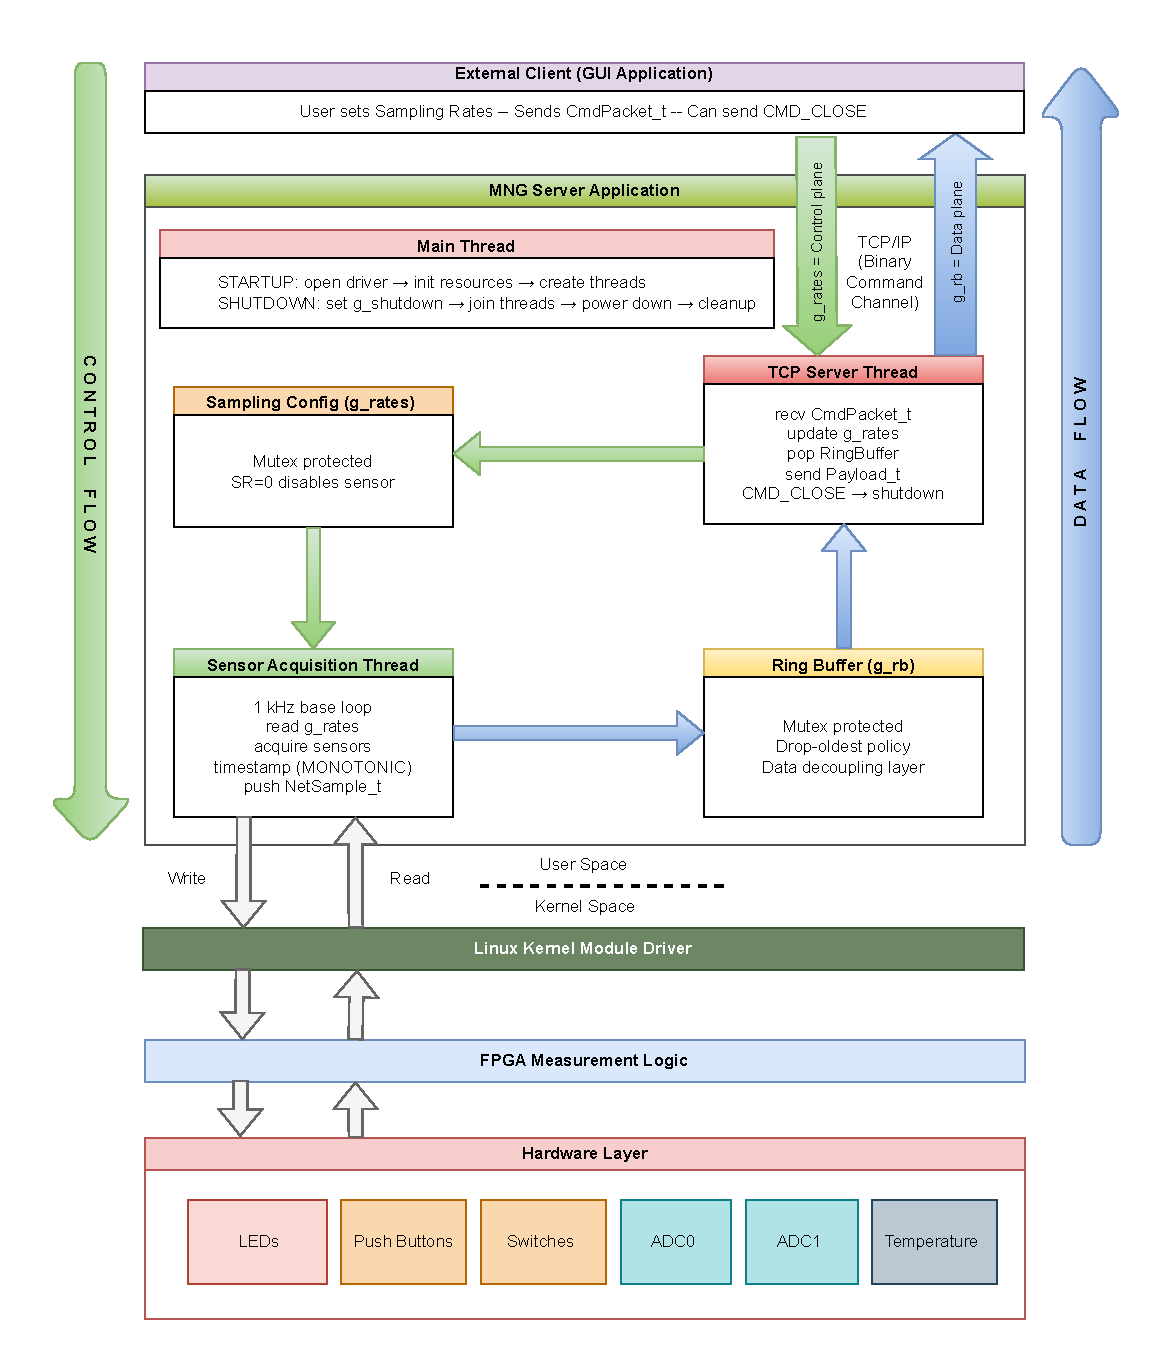
\includegraphics[width=0.9\textwidth]{figures/cmd_get_data_sequence.pdf}
	\caption{Overall software architecture of the Measurement Network Gateway (MNG)}
	\label{fig:mng_architecture}
\end{figure}

Figure~\ref{fig:mng_architecture} illustrates the complete layered architecture of the Measurement Network Gateway (MNG) server system, including the external GUI client, the user-space server application, the Linux kernel driver boundary, the FPGA measurement logic, and the underlying hardware layer. The diagram explicitly distinguishes between the data plane and the control plane, which constitute two orthogonal communication paths within the system.

The data flow propagates upward from the hardware layer toward the external client. Physical measurements originating from temperature sensors, ADC channels, and digital inputs are first processed by the FPGA measurement subsystem and exposed via a register-based interface. The Linux kernel module driver provides a controlled abstraction of this hardware interface through the device node \texttt{/dev/meascdd}. The sensor acquisition thread periodically retrieves measurement values via \texttt{read}/\texttt{write} system calls, timestamps each sample using a monotonic clock source, and pushes the resulting \texttt{NetSample\_t} structures into a mutex-protected ring buffer. The TCP server thread subsequently consumes buffered samples and transmits them to the GUI client using a bounded binary payload.

In contrast, the control flow propagates downward from the GUI client to the acquisition logic. Configuration commands are transmitted via a binary TCP protocol using \texttt{CmdPacket\_t} messages. The TCP thread updates the global sampling-rate configuration structure (\texttt{g\_rates}), which is protected by a mutex to ensure thread-safe concurrent access. The sensor acquisition thread reads this configuration at deterministic cycle boundaries, thereby enabling runtime reconfiguration without interrupting system operation.

A central architectural element is the explicit decoupling between deterministic sampling and asynchronous network communication. The sensor acquisition thread operates at a fixed 1~kHz base rate and derives individual sensor frequencies through integer divisors, thereby maintaining a stable time base. The ring buffer acts as a producer--consumer boundary between acquisition and transmission. By employing a drop-oldest overflow policy, the system ensures that slow or bursty network conditions cannot block time-critical acquisition tasks. This design decision prioritizes temporal consistency and system stability over historical completeness of data, which is appropriate for real-time measurement gateway applications.

The main thread functions exclusively as a lifecycle controller. It performs initialization of shared resources at startup, selects between real hardware mode and synthetic fallback mode, creates worker threads, and supervises cooperative shutdown via a shared termination flag. During shutdown, all threads are joined deterministically, hardware components are powered down where applicable, and all synchronization primitives and file descriptors are released. The clear separation between user space and kernel space, illustrated in the diagram, further emphasizes the layered design philosophy: hardware-specific logic remains encapsulated in the driver layer, while application-level logic operates independently in user space.

Overall, the architecture shown in Figure X.1 demonstrates a structured, modular, and concurrency-aware design that satisfies timing precision, configurability, resource management, and binary protocol efficiency requirements while maintaining clear separation of concerns across all system layers.

\subsection{Protocol and Data Model (Context for Later Sections)}
\label{subsec:protocol-model}

To ensure efficient network transport and compliance with the payload limitation for a single TCP/IP transmission (REQ-17), the server transmits measurements in a strictly binary format (REQ-16). Each measurement is represented as a packed \texttt{NetSample\_t} structure of exactly 14 bytes:

\begin{lstlisting}
	typedef struct __attribute__((packed)) {
		uint64_t time;       // timestamp: microseconds (monotonic)
		uint16_t sensor_id;  // which sensor
		int32_t  value;      // measured value
	} NetSample_t;
	
	#define NETSAMPLE_SIZE 14
\end{lstlisting}

The total size of one sample is therefore:

\[
\text{sizeof(NetSample\_t)} =
8~\text{bytes} + 2~\text{bytes} + 4~\text{bytes}
= 14~\text{bytes}
\]

Each TCP response contains a 32-bit sample counter followed by up to
\( N = 104 \) packed samples:

\begin{lstlisting}
	#define SAMPLES_PER_RESPONSE 104
	
	typedef struct {
		uint32_t count;
		NetSample_t buf[SAMPLES_PER_RESPONSE];
	} Payload_t;
\end{lstlisting}

The maximum payload size is therefore:

\[
\begin{aligned}
	\text{Payload}_{\max}
	&= 4~\text{bytes (count)} + N \cdot 14~\text{bytes} \\
	&= 4 + 104 \cdot 14 \\
	&= 4 + 1456 \\
	&= 1460~\text{bytes}
\end{aligned}
\]

This value is deliberately engineered to remain below the classical
Ethernet MTU constraint of

\[
\text{MTU}_{\text{Ethernet}} = 1500~\text{bytes}
\]

Under standard IPv4/TCP transport, the usable TCP payload per Ethernet frame is:

\[
1500 - 20_{\text{IP header}} - 20_{\text{TCP header}}
= 1460~\text{bytes}
\]

Thus,

\[
\text{Payload}_{\max} = 1460~\text{bytes}
\leq 1500~\text{bytes}
\]

which ensures that each response fits into a single TCP segment under
typical Ethernet conditions, thereby minimizing segmentation overhead
and supporting deterministic transmission behavior.

By using packed binary structures without ASCII conversion or floating-point formatting, the implementation guarantees both compactness and predictable frame sizing, directly satisfying REQ-16 and REQ-17.

\section{Detailed Software Architecture and Concurrency Model}
\label{sec:concurrency}

The internal architecture of the MNG server application is deliberately designed around a strict separation of concerns between time-deterministic sensor acquisition and event-driven network communication. This separation is not merely an implementation detail but a core architectural decision required to satisfy multiple design and RAMS constraints simultaneously. In particular, REQ-14 explicitly requires a multithreaded implementation, while REQ-27 (timing precision and jitter evaluation) implicitly demands that sampling execution must not be blocked or distorted by network delays.

To fulfill these constraints, the application is structured around three concurrent execution contexts:

\begin{itemize}
	\item Main control thread
	\item Sensor acquisition thread
	\item TCP service thread
\end{itemize}

Together, these components form a structured producer--consumer architecture with deterministic timing boundaries.

\begin{figure}[H]
	\centering
	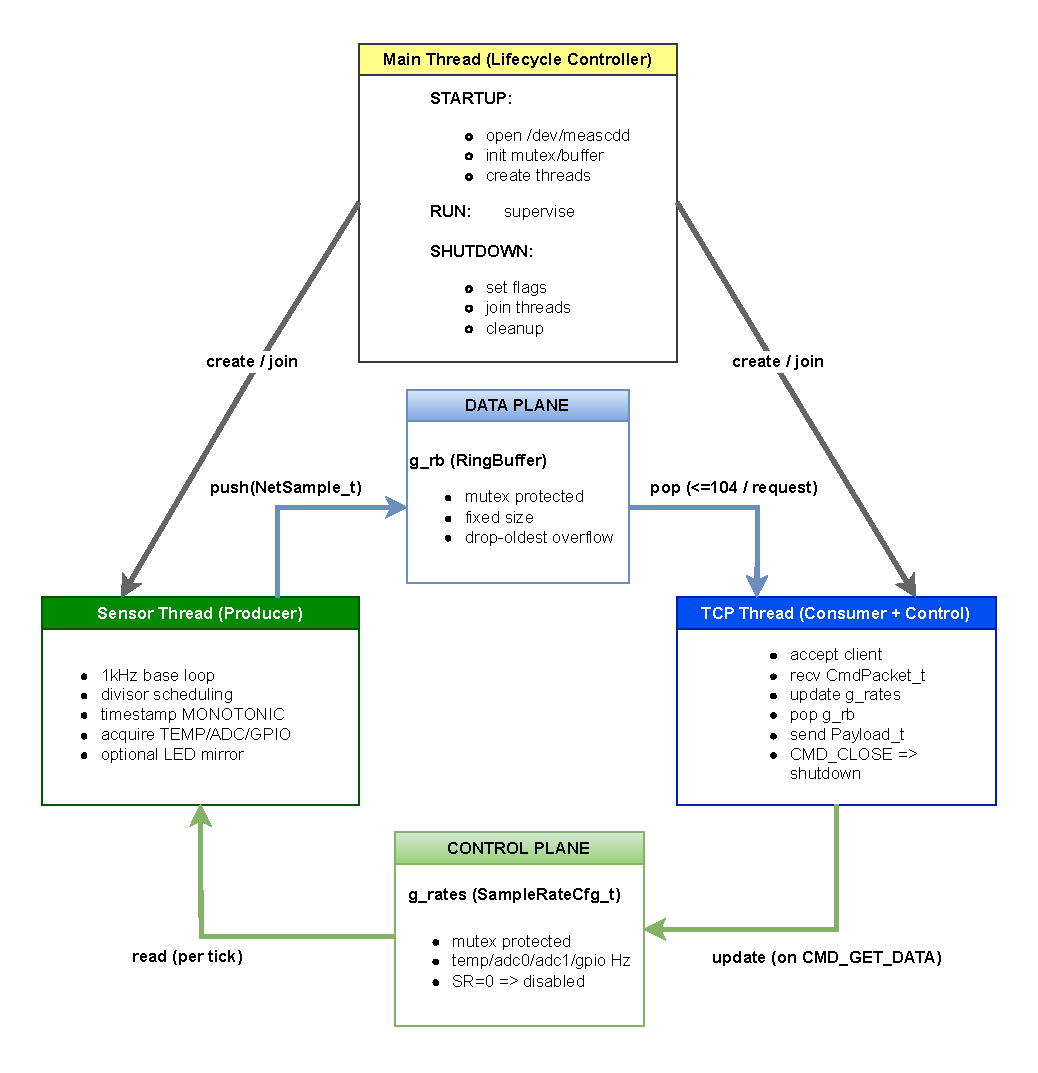
\includegraphics[width=0.95\textwidth]{figures/concurrency_architecture.pdf}
	\caption{Thread interaction model of the MNG server.}
	\label{fig:concurrency-architecture}
\end{figure}
Figure~\ref{fig:concurrency-architecture} illustrates the complete runtime interaction model of the server application. The main thread acts as a lifecycle controller responsible for initialization, supervision, and coordinated shutdown. It creates and joins both worker threads while remaining logically separated from real-time acquisition and network communication responsibilities.

The sensor thread operates as the deterministic producer within the data plane. It executes a fixed 1~kHz base loop, performs divisor-based scheduling, timestamps measurements using a monotonic clock, and pushes \texttt{NetSample\_t} objects into the mutex-protected ring buffer (\texttt{g\_rb}). The ring buffer constitutes the producer--consumer boundary and ensures that acquisition timing remains independent of network conditions.

The TCP thread acts simultaneously as consumer and control interface. It pops buffered samples (up to 104 per request), packages them into a bounded payload, and transmits them over TCP. Additionally, it updates the shared configuration structure (\texttt{g\_rates}) upon receiving \texttt{CMD\_GET\_DATA} commands. This configuration structure forms the control plane and is accessed atomically by both threads via mutex protection.

The explicit separation between data plane and control plane guarantees that configuration updates do not interfere with deterministic sampling. Likewise, the drop-oldest overflow policy prevents network delays from blocking acquisition. The diagram therefore visualizes the architectural principles of concurrency separation, bounded buffering, and cooperative lifecycle control that define the server design.

\subsection{Thread Lifecycle and Responsibility Separation}
\label{subsec:thread-lifecycle}

The \texttt{main()} function serves exclusively as a system orchestrator. It initializes global resources, creates both worker threads, supervises shutdown signaling, and performs deterministic cleanup at termination. Importantly, the main thread itself does not perform sampling nor network communication; this prevents unintended coupling between initialization logic and runtime processing.

Thread creation is realized using POSIX threads:

\begin{lstlisting}
	if (pthread_create(&sensor_th, NULL, sensor_thread, &scfg) != 0) {
		perror("pthread_create(sensor)");
	}
	
	if (pthread_create(&tcp_th, NULL, tcp_thread, NULL) != 0) {
		perror("pthread_create(tcp)");
	}
\end{lstlisting}

The choice of separate threads ensures that blocking socket operations cannot introduce jitter into the deterministic sampling loop.

Shutdown coordination is implemented via a global flag:

\begin{lstlisting}
	static volatile int g_shutdown = 0;
\end{lstlisting}

Both worker threads periodically evaluate this flag and terminate cooperatively. This design avoids abrupt cancellation and satisfies REQ-21.

\subsection{Producer--Consumer Decoupling via Ring Buffer}

A central architectural element of the system is the ring buffer implementation. The ring buffer decouples the deterministic sampling process from the asynchronous network transmission. Its structure is defined as:

\begin{lstlisting}[language=C]
	typedef struct {
		
		pthread_mutex_t mutex;
		
		NetSample_t     buf[RBUF_LEN];
		
		int             head;   // write index
		
		int             tail;   // read index
		
		int             count;  // number of stored elements
		
	} RingBuffer_t;
\end{lstlisting}

The buffer size is fixed at:

\begin{lstlisting}[language=C]
	#define RBUF_LEN 312
\end{lstlisting}

The decision to use a fixed-size circular buffer instead of dynamic allocation is intentional. In embedded Linux environments, predictable memory behavior is preferred over dynamic allocation at runtime, particularly in long-running processes. This avoids heap fragmentation and aligns with RAMS considerations regarding system stability.

The push operation demonstrates a deliberate overflow policy:

\begin{lstlisting}[language=C]
	if (rb->count == RBUF_LEN) {
		
		rb->tail = (rb->tail + 1) % RBUF_LEN;  // drop oldest
		
	} else {
		
		rb->count++;
		
	}
\end{lstlisting}

Instead of blocking when the buffer is full, the system discards the oldest sample. This policy ensures that the sampling thread never blocks due to slow network consumption. From a systems perspective, this choice prioritizes real-time acquisition continuity over historical completeness. In measurement gateway applications, maintaining current data flow is often more critical than preserving outdated samples.

The pop operation is non-blocking:

\begin{lstlisting}[language=C]
	if (rb->count == 0) {
		
		pthread_mutex_unlock(&rb->mutex);
		
		return 0;
		
	}
\end{lstlisting}

This design prevents the TCP thread from blocking indefinitely when no data is available. Instead, it simply returns zero samples, and the client receives an empty response. This behavior maintains responsiveness and supports REQ-26 (testability) by allowing observation of system behavior even under idle conditions.

\subsection{Timing Strategy and Deterministic Sampling}

One of the most important architectural aspects of the server is its deterministic timing model. The sensor thread operates on a fixed base loop frequency:

\begin{lstlisting}[language=C]
	#define BASE_RATE_HZ 1000u
\end{lstlisting}

This defines a 1 kHz base sampling tick (1 ms period). Instead of running each sensor independently, all sensor activities are derived from this base tick using integer divisors:

\begin{lstlisting}[language=C]
	uint32_t temp_div = (temp_hz > 0) ? (BASE_RATE_HZ / temp_hz) : 0;
\end{lstlisting}

This design has several advantages:

\begin{itemize}
	\item All sampling operations are synchronized to a common time base.
	\item Sampling frequency changes can be applied dynamically.
	\item Relative timing between sensors remains deterministic.
\end{itemize}

The base loop delay is implemented using \texttt{nanosleep}:

\begin{lstlisting}[language=C]
	struct timespec req;
	
	req.tv_sec  = 0;
	
	req.tv_nsec = 1 * 1000000L;  // 1 ms
	
	nanosleep(&req, NULL);
\end{lstlisting}

While \texttt{nanosleep} does not provide hard real-time guarantees under standard Linux scheduling, it is sufficient for soft real-time measurement applications in Embedded Linux environments. Furthermore, jitter can be evaluated using timestamps (REQ-27).

\subsection{Timestamping and Temporal Consistency}

Every measurement is timestamped using the monotonic clock:

\begin{lstlisting}[language=C]
	static uint64_t get_time_us(void)
	{
		struct timespec ts;
		
		clock_gettime(CLOCK_MONOTONIC, &ts);
		
		return (uint64_t)ts.tv_sec * 1000000ull + ts.tv_nsec / 1000ull;
	}
\end{lstlisting}

The use of CLOCK MONOTONIC instead of CLOCK REALTIME is a deliberate design decision. Real-time clocks may be adjusted by the system (e.g., NTP synchronization), which would introduce discontinuities in measurement time. In contrast, the monotonic clock guarantees strictly increasing timestamps independent of wall-clock corrections. This ensures temporal consistency and supports accurate delay and jitter evaluation (REQ-27).

The timestamp is stored directly inside each transmitted sample:

\begin{lstlisting}[language=C]
	pkt.time = time;
\end{lstlisting}

Thus, every measurement is self-contained and temporally traceable, fully satisfying REQ-8.

\subsection{Sample Rate Configuration Mechanism}

Sampling rates are stored in a mutex-protected global configuration structure:

\begin{lstlisting}[language=C]
	typedef struct {
		
		pthread_mutex_t mutex;
		
		uint32_t temp_hz;
		
		uint32_t adc0_hz;
		
		uint32_t adc1_hz;
		
		uint32_t gpio_hz;
		
	} SampleRateCfg_t;
\end{lstlisting}

This design allows dynamic reconfiguration without restarting the application. The TCP thread updates the configuration when receiving a \texttt{CMD\_GET\_DATA} packet:

\begin{lstlisting}[language=C]
	pthread_mutex_lock(&g_rates.mutex);
	
	g_rates.temp_hz = sr_temp;
	
	g_rates.adc0_hz = sr_adc0;
	
	g_rates.adc1_hz = sr_adc1;
	
	g_rates.gpio_hz = sr_gpio;
	
	pthread_mutex_unlock(&g_rates.mutex);
\end{lstlisting}

The sensor thread reads the configuration atomically at each base tick. This ensures that configuration changes are applied deterministically at the next cycle boundary.

A sample rate of zero is interpreted as disabled:

\begin{lstlisting}[language=C]
	uint32_t temp_div = (temp_hz > 0) ? (BASE_RATE_HZ / temp_hz) : 0;
\end{lstlisting}

This implementation satisfies:

\begin{itemize}
	\item REQ-6 (configurable sampling rate per signal)
	\item REQ-7 (selectable sensors)
	\item REQ-9 and REQ-10 (configuration via control program)
\end{itemize}

\section{Hardware Interaction Layer and Kernel Driver Communication}

The hardware interaction layer of the MNG server represents the boundary between user-space software and FPGA-based measurement logic. This layer is responsible for translating high-level measurement requests into register-level transactions via the Linux kernel driver (/dev/meascdd). It is implemented entirely in user space but relies on a structured data exchange mechanism \texttt{MeasObj\_struct} that abstracts register-based communication with the FPGA subsystem.

This architectural separation ensures that hardware-specific access logic remains encapsulated within the kernel module, while the server application operates at a higher abstraction level. Such layering improves portability, modularity, and maintainability, and it aligns with good embedded Linux design practice.

\subsection{Driver Interface and Register Transaction Model}

Communication with the FPGA measurement subsystem is performed using the following structure:

\begin{lstlisting}[language=C]
	typedef struct {
		
		unsigned int rnum;
		
		unsigned int rvalue;
		
	} MeasObj_struct;
\end{lstlisting}

Each transaction consists of:

\begin{itemize}
	\item A register number (rnum)
	\item A register value (rvalue)
\end{itemize}

Data exchange is performed using standard write() and read() system calls on the device node:

\begin{lstlisting}[language=C]
	ret = write(fd, &TF_Obj_Snd, MEASOBJ_SIZE);
	
	ret = read(fd, &TF_Obj_Rcv, MEASOBJ_SIZE);
\end{lstlisting}

This approach satisfies REQ-13 (Embedded Linux) by using standard POSIX system calls rather than custom kernel hooks. It also ensures binary communication without ASCII conversion (REQ-16).

The constant:

\begin{lstlisting}[language=C]
	#define REGNUM_ID 0x0FF
\end{lstlisting}

is used as a polling register identifier to query hardware status flags. The driver-level polling loop in MaxRead() demonstrates a synchronous register transaction model:

\begin{lstlisting}[language=C]
	do {
		
		TF_Obj_Snd.rnum   = REGNUM_ID;
		
		TF_Obj_Snd.rvalue = 1;
		
		write(fd, &TF_Obj_Snd, MEASOBJ_SIZE);
		
		read(fd, &TF_Obj_Rcv, MEASOBJ_SIZE);
		
		xdata = TF_Obj_Rcv.rvalue;
		
	} while (((xdata & 0x01) == 0) && (k < 1000));
\end{lstlisting}

The loop waits until a hardware-ready flag becomes set or a timeout occurs. This polling-based approach simplifies synchronization and avoids interrupt-driven complexity in user space.

\subsection{Temperature Acquisition (MAX31865 – REQ-2)}

Temperature measurement is performed using a precision resistive temperature sensor connected through a MAX31865 interface. The acquisition process includes:

\begin{itemize}
	\item Power-up and initialization
	\item Conversion start
	\item Status polling
	\item MSB/LSB register read
	\item 15-bit raw value extraction
\end{itemize}

Initialization sequence:

\begin{lstlisting}[language=C]
	static void PMB1_Init(int fd)
	{
		TF_Obj_Snd.rnum   = 0;
		
		TF_Obj_Snd.rvalue = 0x022;
		
		write(fd, &TF_Obj_Snd, MEASOBJ_SIZE);
		
		MaxWrite(fd, 0x00, 0x081);   // power up MAX31865
	}
\end{lstlisting}

Conversion start:

\begin{lstlisting}[language=C]
	MaxWrite(fd, 0x00, 0x0a1);  // start conversion
\end{lstlisting}

Data readout:

\begin{lstlisting}[language=C]
	xdata = MaxRead(fd, 0x01);   // MSB
	
	xdata <<= 8;
	
	xlsb  = MaxRead(fd, 0x02);   // LSB
	
	xdata |= (xlsb & 0xff);
	
	xadc = xdata >> 1;
\end{lstlisting}

The raw ADC value is intentionally transmitted without floating-point conversion. This design decision preserves precision and ensures that no ASCII or float formatting is performed before network transmission (REQ-16). Temperature conversion to physical units can be performed on the client side if required.

Power-down is explicitly handled during shutdown:

\begin{lstlisting}[language=C]
	MaxWrite(cfg->fd, 0x00, 0x001); // power down PMB1
\end{lstlisting}

This fulfills REQ-20 (disable sensors on termination).

\subsection{ADC Acquisition (REQ-3)}

The system captures data from two ADC channels via a PmodAD1 module. Both channels are acquired simultaneously in a single 32-bit word:

\begin{lstlisting}[language=C]
	*adc0 = (uint16_t)(adc_word & 0x0fff);
	
	*adc1 = (uint16_t)((adc_word >> 16) & 0x0fff);
\end{lstlisting}

Each channel is 12-bit wide. The server keeps the channels logically separated using different \texttt{sensor\_id} values:

\begin{lstlisting}[language=C]
	#define SENSOR_ID_ADC0 2
	
	#define SENSOR_ID_ADC1 3
\end{lstlisting}

Although acquisition is simultaneous at hardware level, transmission is decoupled logically. Each ADC channel is treated as an independent sensor stream, enabling independent sampling rate configuration (REQ-6).

\subsection{Digital Inputs: Switches and Pushbuttons (REQ-4, REQ-5)}

Digital input acquisition is performed via register 0:

\begin{lstlisting}[language=C]
	*switches = (uint8_t)(val & 0xff);
	
	*pushb    = (uint8_t)((val >> 8) & 0x1f);
\end{lstlisting}

The design combines both into a single logical sensor group:

\begin{lstlisting}[language=C]
	pkt.sensor_id = SENSOR_ID_GPIO;
	
	pkt.value = ((int32_t)pb_state << 8) | (int32_t)sw_state;
\end{lstlisting}

This compact encoding reduces payload size and ensures efficient transmission. It also satisfies REQ-25, which specifies that switches and push buttons shall be used as auxiliary digital input signals.

\subsection{LED Mirror Feature (Optional Enhancement)}

An additional feature implemented in the sensor thread mirrors switch states to onboard LEDs:

\begin{lstlisting}[language=C]
	Write_LEDs(cfg->fd, sw_state);
\end{lstlisting}

This functionality is not explicitly required in the requirements specification but represents a valuable diagnostic feature. It provides immediate visual feedback that confirms correct GPIO readout and driver interaction. Such features improve testability and development efficiency, especially in early integration phases.

\subsection{Fake Sensor Mode (Design Enhancement)}

If /dev/meascdd cannot be opened, the system automatically switches to a synthetic signal generator mode:

\begin{lstlisting}[language=C]
	if (fd < 0) {
		
		use_fake_sensor = 1;
		
	}
\end{lstlisting}

In fake mode:

\begin{itemize}
	\item ADC values are generated as sine waves
	\item Temperature increases incrementally
	\item GPIO values default to zero
\end{itemize}

Example sine generation:

\begin{lstlisting}[language=C]
	double v0 = offset + amp * sin(2.0 * M_PI * 2.0 * t);
\end{lstlisting}

This feature is particularly valuable for:

\begin{itemize}
	\item Offline GUI development
	\item Network testing without hardware
	\item Timing analysis under controlled conditions
\end{itemize}

Although not explicitly required, this functionality strongly supports REQ-26 (functional testing).

\section{TCP Communication Protocol and Binary Payload Design}

The network communication layer of the MNG server is implemented as a TCP/IP service that exposes measurement data to a remote control computer. The design adopts a command/response paradigm rather than a continuous streaming paradigm. This decision is motivated by the need for explicit control over which sensors are active and at what rates they are sampled, as well as by the requirement to keep each TCP transmission within a fixed maximum payload size. In the overall system, the MNG acts as a TCP server while the control computer acts as the TCP client (REQ-1). Consequently, network interaction is initiated by the client, which sends configuration commands and requests data, while the server responds with a bounded set of measurements collected since the last request.

Two goals dominate the protocol design: first, all data exchange must occur in strictly binary form to avoid conversion overhead and preserve compactness (REQ-16). Second, each response must be designed such that it fits into a single Ethernet frame whenever possible, thereby complying with the maximum payload constraint of 1500 bytes (REQ-17) and improving performance by avoiding fragmentation and unnecessary protocol overhead. The implementation explicitly targets approximately one TCP segment worth of data per request.

\subsection{Server Socket Setup and Connection Lifecycle}

The server binds to a fixed TCP port and waits for a single client connection. The socket setup is conventional but deliberately configured for robust restart behavior via \texttt{SO\_REUSEADDR}, which prevents “address already in use” errors after an abnormal termination or a fast restart during development:

\begin{lstlisting}[language=C]
	srv_fd = socket(AF_INET, SOCK_STREAM, 0);
	
	int opt = 1;
	
	setsockopt(srv_fd, SOL_SOCKET, SO_REUSEADDR, &opt, sizeof(opt));
	
	addr.sin_family      = AF_INET;
	
	addr.sin_addr.s_addr = htonl(INADDR_ANY);
	
	addr.sin_port        = htons(TCP_PORT);
	
	bind(srv_fd, (struct sockaddr *)&addr, sizeof(addr));
	
	listen(srv_fd, 1);
	
	cli_fd = accept(srv_fd, (struct sockaddr *)&cli_addr, &cli_len);
\end{lstlisting}

The design uses a single connection model (listen backlog of 1), which is sufficient for the intended laboratory and demonstration scenario where a single control computer interacts with the MNG at a time. Importantly, if the client disconnects or requests termination, the server transitions into a controlled shutdown sequence. This behavior is consistent with RAMS expectations because it avoids leaving worker threads running in an undefined state.

Client disconnect detection is handled via recv() returning 0 bytes, which is the standard TCP indication of an orderly shutdown by the peer:

\begin{lstlisting}[language=C]
	ssize_t n = recv(cli_fd, &cmd, sizeof(cmd), MSG_WAITALL);
	
	if (n == 0) {
		
		printf("[tcp] client closed connection.\n");
		
		g_shutdown = 1;
		
		break;
		
	}
\end{lstlisting}

The same shutdown flag is also set on error conditions, ensuring that network failures lead to a predictable and safe termination path rather than undefined behavior.

\subsection{Command Packet Format and Semantic Meaning}

Figure~\ref{fig:cmd_get_data_sequence} illustrates the complete interaction sequence between the GUI client, the TCP server thread, the sensor thread, the shared ring buffer, and the kernel driver during a \texttt{CMD\_GET\_DATA} request/response cycle.

\begin{figure}[H]
	\centering
	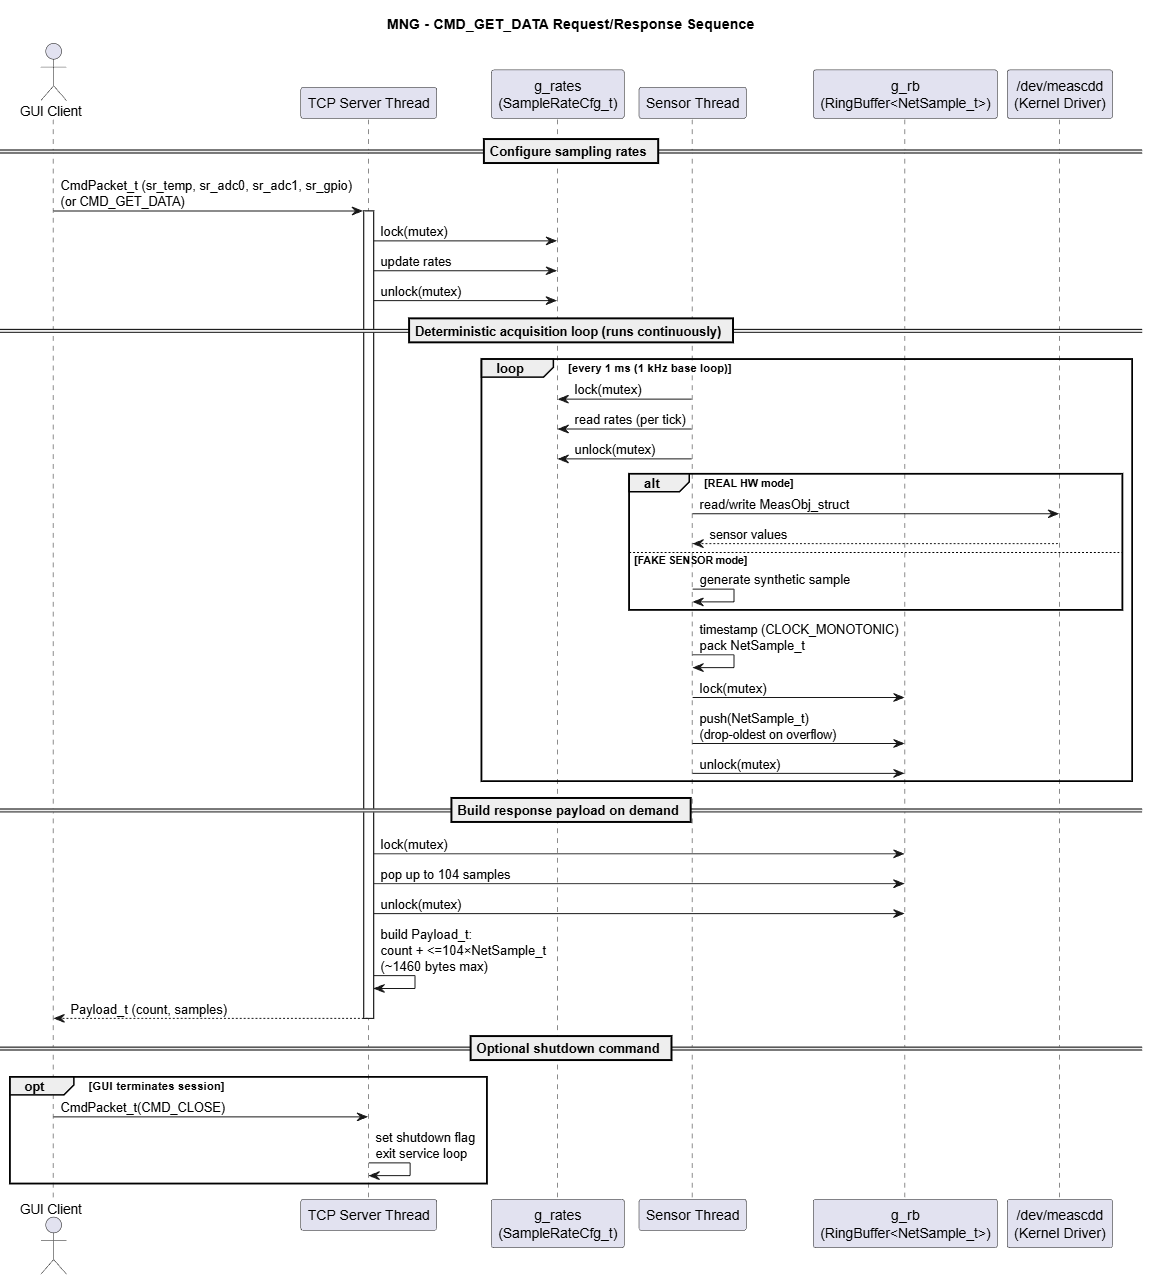
\includegraphics[width=\textwidth]{figures/cmd_get_data_sequence.png}
	\caption{UML Sequence Diagram of the CMD\_GET\_DATA Request/Response Cycle}
	\label{fig:cmd_get_data_sequence}
\end{figure}

The client interacts with the server by sending a fixed-size command structure, \texttt{CmdPacket\_t}, which is explicitly designed as a binary control message:

\begin{lstlisting}[language=C]
	typedef struct __attribute__((packed)) {
		
		uint32_t cmd;      // command code
		
		uint32_t sr_temp;  // TEMP sample rate (Hz)
		
		uint32_t sr_adc0;  // ADC0 sample rate (Hz)
		
		uint32_t sr_adc1;  // ADC1 sample rate (Hz)
		
		uint32_t sr_gpio;  // GPIO sample rate (Hz)
		
	} CmdPacket_t;         // 20 bytes
\end{lstlisting}

Two command codes are implemented:

\begin{lstlisting}[language=C]
	#define CMD_GET_DATA 1
	
	#define CMD_CLOSE    2
\end{lstlisting}

From a protocol perspective, \texttt{CMD\_GET\_DATA} serves a dual purpose. First, it carries the client’s desired sampling rates for each sensor. Second, it acts as a “data request trigger,” instructing the server to respond immediately with a bounded set of samples currently available in the ring buffer. This coupling of configuration and request into a single packet keeps the protocol minimal and avoids extra message exchanges, which further reduces overhead.

The \texttt{CMD\_CLOSE} command enables controlled shutdown initiated by the client. This command is important for meeting REQ-18 and REQ-21 because it ensures the application can terminate cleanly under software control without relying on abrupt termination (e.g., forced kill).

\subsection{Dynamic Reconfiguration of Sampling Rates (Cross-Layer Interaction)}

Upon receiving a \texttt{CMD\_GET\_DATA} request, the TCP thread updates the global sampling-rate configuration. Because the sensor thread reads these rates continuously, a mutex is used to guarantee consistent updates:

\begin{lstlisting}[language=C]
	pthread_mutex_lock(&g_rates.mutex);
	
	g_rates.temp_hz = sr_temp;
	
	g_rates.adc0_hz = sr_adc0;
	
	g_rates.adc1_hz = sr_adc1;
	
	g_rates.gpio_hz = sr_gpio;
	
	pthread_mutex_unlock(&g_rates.mutex);
\end{lstlisting}

This mechanism realizes a runtime reconfiguration capability: a remote client can enable or disable sensors and adjust their sampling frequencies on-the-fly without restarting the server. A sampling rate of zero is interpreted as ``disabled,'' which effectively implements sensor selectability (REQ-7) and sampling rate configurability (REQ-6) using the same configuration path. In the larger system context, the GUI will act as this control client (REQ-9, REQ-10), while the terminal-based test client provides an additional verification path (REQ-26).

\subsection{Response Payload Format and Size Engineering}

The server responds using a payload container that begins with a 32-bit count field followed by count packed samples:

\begin{lstlisting}[language=C]
	typedef struct {
		
		uint32_t   count;
		
		NetSample_t buf[SAMPLES_PER_RESPONSE];
		
	} Payload_t;
\end{lstlisting}

Each sample is defined as a packed 14-byte structure:

\begin{lstlisting}[language=C]
	typedef struct __attribute__((packed)) {
		
		uint64_t time;
		
		uint16_t sensor_id;
		
		int32_t  value;
		
	} NetSample_t;
\end{lstlisting}

\begin{lstlisting}[language=C]
	#define NETSAMPLE_SIZE 14
\end{lstlisting}

The constant \texttt{SAMPLES\_PER\_RESPONSE} is set to 104:

\begin{lstlisting}[language=C]
	#define SAMPLES_PER_RESPONSE 104
\end{lstlisting}

The choice of 104 is not arbitrary. The payload is engineered so that the maximum transmitted size remains below the classical Ethernet MTU threshold. Specifically, the payload size is:

\begin{itemize}
	\item 4 bytes for \texttt{count}
	\item 104 × 14 = 1456 bytes for samples
	\item Total = 1460 bytes
\end{itemize}

This explicitly meets the design requirement that the payload for a single TCP/IP transmission is limited to 1500 bytes (REQ-17). Additionally, by using packed binary structures without ASCII conversion, it satisfies REQ-16.

This is also reflected in the comment embedded in the header:

\begin{lstlisting}[language=C]
	#define SAMPLES_PER_RESPONSE  104   // 4 + 104 * 14 = 1460 bytes (~one TCP segment)
\end{lstlisting}

Packet inspection using Wireshark confirmed that transmitted TCP segments remained below the Ethernet MTU and no IP fragmentation occurred during testing.

From a performance perspective, keeping the payload close to (but below) the typical MTU improves efficiency because it tends to be transmitted as a single TCP segment with minimal fragmentation. While TCP segmentation and IP fragmentation are handled by the stack, avoiding them is beneficial for deterministic timing behavior and overall throughput, particularly in embedded systems where CPU budget and memory copies are non-trivial.

\subsection{Response Generation Logic and Ring Buffer Consumption}

When a \texttt{CMD\_GET\_DATA} is received, the TCP thread attempts to pop up to 104 samples from the ring buffer. The server does not block waiting for data; instead, it returns what is immediately available. This design choice ensures that the client’s request/response cycle remains bounded in time, which is important when the control program (GUI) is expected to refresh live data at interactive rates.

The pop and response filling logic is implemented as:

\begin{lstlisting}[language=C]
	for (int i = 0; i < SAMPLES_PER_RESPONSE; ++i) {
		
		NetSample_t pkt;
		
		if (RingBuffer_pop(&g_rb, &pkt)) {
			g_pl.buf[i] = pkt;
			g_pl.count = g_pl.count + 1;
		} else {
			break;
		}
	}
\end{lstlisting}

If no samples are available, the server sends only the count field (which is zero). This is a deliberate micro-optimization: it avoids sending a full payload with meaningless data and clearly indicates an “empty response” to the client:

\begin{lstlisting}[language=C]
	if (g_pl.count == 0) {
		send(cli_fd, &g_pl.count, sizeof(uint32_t), 0);
	} else {
		send(cli_fd, &g_pl, (sizeof(uint32_t) + (g_pl.count * NETSAMPLE_SIZE)), 0);
	}
	
	g_pl.count = 0;
\end{lstlisting}

A noteworthy point in the implementation is the dummy samples. During development the system considered an alternative strategy where responses could always contain a fixed number of samples by padding with “dummy” entries when the ring buffer is empty. Ultimately, the implemented approach of variable-length responses is more bandwidth-efficient and semantically cleaner, because the client can directly interpret \texttt{count = 0} as “no data available.”

\subsection{Protocol Characteristics: Determinism, Efficiency, and Extensibility}

The implemented protocol exhibits three important characteristics. First, it is deterministic in the sense that response size is bounded and command processing remains lightweight, which reduces jitter induced by network handling. Second, it is efficient: by avoiding ASCII conversions and by sizing responses to fit into a single near-MTU payload, CPU overhead and network overhead are minimized. Third, it remains extensible: additional sensors or additional commands could be introduced by extending the \texttt{sensor\_id} namespace and adding new command codes, while keeping backward compatibility as long as structure sizes and packing rules are preserved.

One subtle but relevant engineering aspect is endianness: because both client and server are intended to run on common little-endian architectures in the lab environment, the code currently sends packed structs without explicit htonl() conversion for fields inside the payload. In a broader deployment scenario with heterogeneous architectures, it would be advisable to define a canonical network byte order for all multi-byte fields to ensure portability. For the intended scope of this project (embedded board + PC), the direct binary transfer is a valid and pragmatic performance optimization aligned with REQ-16.

\section{Startup/Shutdown Procedures, RAMS Compliance, and Resource Management}

A robust embedded measurement gateway must not only deliver correct functional behavior but also provide deterministic startup and shutdown procedures, ensuring that the system can be brought into operation reliably and terminated without leaving the hardware in an undefined state or the software in a resource-leaking condition. In the context of this project, these concerns are formalized in the RAMS requirements (REQ-18 to REQ-21). The MNG server application implements an explicit lifecycle model covering (i) initialization of all required resources at startup, (ii) cooperative termination across threads, (iii) sensor deactivation at shutdown, and (iv) destruction of allocated resources prior to process exit.

The central design principle behind the implemented lifecycle is cooperative shutdown: instead of abruptly cancelling threads or relying on external process termination, a global shutdown flag coordinates termination across all execution contexts. This reduces the risk of leaving the driver interface in an inconsistent state, avoids deadlocks due to forced cancellation during mutex holds, and ensures that finalization actions (such as powering down sensors) are executed deterministically.

\subsection{Controlled Startup Sequence (REQ-18, REQ-19)}

At startup, the program performs a sequence of initialization steps that ensures the system enters a defined operational state before accepting any client interaction. The initialization begins by attempting to open the kernel driver device node:

\begin{lstlisting}[language=C]
	fd = open("/dev/meascdd", O_RDWR);
	
	if (fd < 0) {
		
		perror("open(/dev/meascdd)");
		
		printf("=> /dev/meascdd not found, running in FAKE SENSOR mode.\n");
		
		use_fake_sensor = 1;
		
	} else {
		
		printf("=> /dev/meascdd opened successfully, REAL HW mode.\n");
		
		use_fake_sensor = 0;
		
	}
\end{lstlisting}

This step is crucial because it defines whether the system will operate against real hardware or in a synthetic fallback mode. Importantly, the fallback is implemented as a deliberate design feature rather than an error condition that prevents operation. This significantly improves availability and supports development and test activities when the hardware stack is temporarily unavailable.

Following device initialization, the application initializes the ring buffer and synchronization primitives:

\begin{lstlisting}[language=C]
	RingBuffer_init(&g_rb);
	
	pthread_mutex_init(&g_rates.mutex, NULL);
	
	g_rates.temp_hz  = 0;
	
	g_rates.adc0_hz  = 0;
	
	g_rates.adc1_hz  = 0;
	
	g_rates.gpio_hz  = 0;
\end{lstlisting}

This ensures that all shared resources exist in a defined initial state before any worker thread begins execution. In particular, initializing sample rates to zero has an important semantic meaning: it ensures that, immediately after startup, no sensor sampling is performed until explicitly requested by the client. This is a safe default because it prevents unintended activity on the driver interface and avoids unnecessary resource usage. Conceptually, the system starts in an “idle acquisition” state and transitions into active acquisition only when commanded.

Finally, the worker threads are created:

\begin{lstlisting}[language=C]
	if (pthread_create(&sensor_th, NULL, sensor_thread, &scfg) != 0) { ... }
	
	if (pthread_create(&tcp_th, NULL, tcp_thread, NULL) != 0) { ... }
\end{lstlisting}

Thread creation is performed after resource initialization to prevent race conditions where a thread might access uninitialized memory or mutexes. This directly addresses REQ-19 (“On startup all resources shall be initialized”).

\subsection{Shutdown Trigger Paths and Cooperative Termination (REQ-18)}

The application supports multiple shutdown triggers. The most important trigger is an explicit client request via the \texttt{CMD\_CLOSE} command. When the TCP thread receives this command, it sets the global shutdown flag and exits the communication loop:

\begin{lstlisting}[language=C]
	if (cmd_code == CMD_CLOSE) {
		
		printf("[tcp] CMD_CLOSE received, closing connection.\n");
		
		g_shutdown = 1;
		
		break;
		
	}
\end{lstlisting}

Additionally, shutdown is triggered if the client closes the TCP connection:

\begin{lstlisting}[language=C]
	if (n == 0) {
		
		printf("[tcp] client closed connection.\n");
		
		g_shutdown = 1;
		
		break;
		
	}
\end{lstlisting}

This ensures that unexpected client termination does not leave the server in a hanging state. The same principle applies to network errors; the TCP thread sets the shutdown flag and terminates, which in turn triggers global shutdown coordination.

The main thread continuously monitors the shutdown flag in a lightweight sleep loop:

\begin{lstlisting}[language=C]
	while (!g_shutdown) {
		
		struct timespec ts;
		
		ts.tv_sec  = 0;
		
		ts.tv_nsec = 200 * 1000000L; // 200 ms
		
		nanosleep(&ts, NULL);
		
	}
\end{lstlisting}

Once shutdown is requested, the main thread signals the sensor thread to stop by clearing its running flag:

\begin{lstlisting}[language=C]
	scfg.running = 0;
\end{lstlisting}

This dual-condition stopping model is important: the sensor thread checks both scfg.running and the global \texttt{g\_shutdown}. This provides a clean mechanism for termination even if shutdown is initiated by internal errors rather than client commands.

\subsection{Sensor Deactivation at Termination (REQ-20)}

A key RAMS requirement is that, upon termination of the application, all sensors must be disabled, including powering down hardware where applicable (REQ-20). In this implementation, the temperature sensor interface (MAX31865 / PMB1) is explicitly powered down inside the sensor thread termination path:

\begin{lstlisting}[language=C]
	if (!use_fake_sensor) {
		
		MaxWrite(cfg->fd, 0x00, 0x001); // power down PMB1
		
	}
\end{lstlisting}

Placing the power-down logic in the sensor thread is architecturally consistent because that thread owns the sensor lifecycle and performs initialization via \texttt{PMB1\_Init()} in its startup path. This symmetry reduces the risk of inconsistent sensor states: initialization and finalization occur in the same execution context, and the same driver file descriptor is used throughout.

This design ensures that hardware is not left in a conversion-active state after user-space termination, which would otherwise be a potential reliability risk (e.g., additional power dissipation, undefined register states, or misleading measurements).

\subsection{Resource Destruction and Thread Join Strategy (REQ-21)}

Another central RAMS requirement is that all allocated resources must be destroyed and all threads must terminate cleanly (REQ-21). The implementation explicitly performs \texttt{pthread\_join()} on both worker threads:

\begin{lstlisting}[language=C]
	pthread_join(sensor_th, NULL);
	
	pthread_join(tcp_th, NULL);
\end{lstlisting}

This ensures that the main thread waits for the controlled completion of both worker threads before proceeding with resource destruction. Such an approach avoids “detached thread” scenarios where the process might exit while threads still hold resources or interact with hardware.

After thread completion, the ring buffer mutex and other synchronization resources are destroyed:

\begin{lstlisting}[language=C]
	RingBuffer_destroy(&g_rb);
\end{lstlisting}

Finally, the device node file descriptor is closed if the application was running in real hardware mode:

\begin{lstlisting}[language=C]
	if (!use_fake_sensor && fd >= 0) close(fd);
\end{lstlisting}

Similarly, within the TCP thread, the server and client sockets are closed as part of its termination path:

\begin{lstlisting}[language=C]
	if (cli_fd >= 0) close(cli_fd);
	
	if (srv_fd >= 0) close(srv_fd);
\end{lstlisting}

This explicit resource cleanup ensures that:

\begin{itemize}
	\item no mutex remains allocated,
	\item no thread remains running,
	\item no file descriptor remains open,
	\item and the OS can reclaim all resources deterministically.
\end{itemize}

Collectively, these mechanisms satisfy REQ-21 and demonstrate a RAMS-oriented design discipline appropriate for embedded systems.

\subsection{Discussion: Why Cooperative Shutdown Improves System Stability}

From a reliability perspective, cooperative shutdown is a safer model than forced termination. In multi-threaded applications, asynchronous thread cancellation can interrupt execution while a thread holds a mutex or is in the middle of a driver transaction, potentially causing deadlocks or corrupt shared state. By using a shared shutdown flag and allowing threads to exit their loops naturally, the system ensures that critical sections are exited cleanly and that hardware is returned to a known state. This is particularly important when interacting with a kernel driver and external hardware, as undefined shutdown states can lead to sporadic failures that are difficult to debug and may negatively affect subsequent startups.

\section{Verification Strategy and Experimental Validation}

The validation of the Measurement Network Gateway server was not limited to static code inspection or architectural reasoning. In order to demonstrate full functional correctness, timing behavior, protocol compliance, and robustness under runtime configuration changes, a dedicated terminal-based test client was developed. This client communicates directly with the server using the defined binary TCP protocol and therefore allows isolated verification of the server application independently from the graphical user interface.

The verification strategy follows a systematic approach in which each requirement category—functional, design, RAMS, and test—is validated through controlled experimental interaction with the running server. The test client operates as an interactive control interface and simultaneously as a diagnostic monitoring tool that exposes raw timestamped measurement samples. This dual role makes it especially suitable for deep behavioral analysis.

\subsection{Experimental Setup and Operational Context}

The verification experiments were conducted by running the MNG server application and the terminal-based test client on the same Linux system, communicating over the loopback interface (127.0.0.1). In this configuration, the server operates either in real hardware mode (when /dev/meascdd is available) or in synthetic signal mode if the device node cannot be opened.

In the presented test scenario, the server automatically switched to fake sensor mode due to the absence of the hardware driver. This behavior is not an error condition but an intentionally designed fallback mechanism. The synthetic mode generates deterministic sine wave signals for ADC channels and incremental values for temperature measurements. This controlled signal generation enables precise verification of sampling logic, timestamp consistency, and data transmission integrity without hardware dependencies.

\begin{figure}[H]
	\centering
	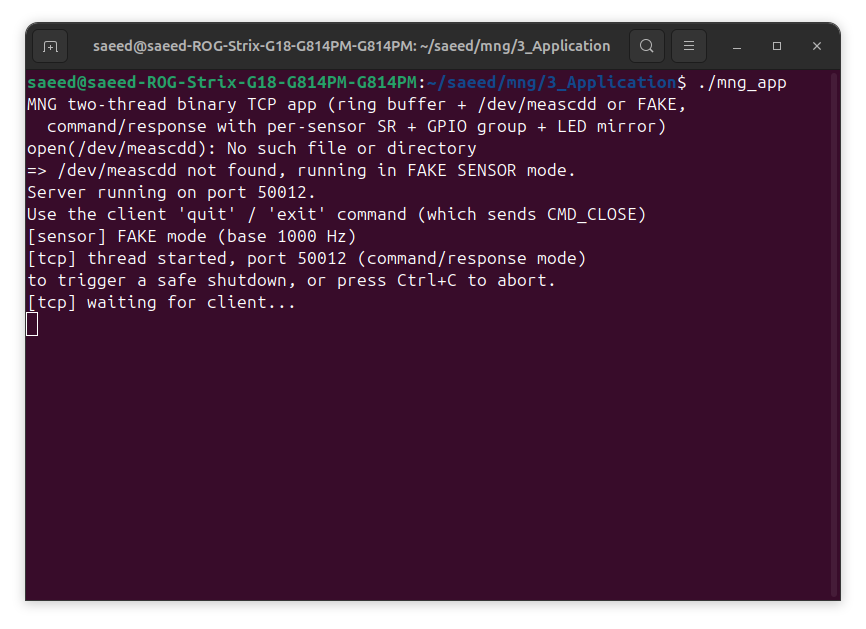
\includegraphics[width=0.9\textwidth]{figures/fig_server_startup_fake_mode.png}
	\caption{Server startup in fake sensor mode and TCP listener initialization.}
	\label{fig:server_startup_fake_mode}
\end{figure}

The console output confirms successful thread creation, activation of the TCP server, and readiness to accept incoming client connections. The absence of hardware therefore does not prevent validation of architectural and protocol-level requirements.

\subsection{Runtime Configuration and Sensor Selection Validation}

One of the key functional requirements (REQ-6 and REQ-7) states that each sensor shall have an independently configurable sampling rate and that sensors must be selectable. This behavior is validated experimentally by configuring only ADC0 to operate at 100 Hz while all other sensors remain disabled (0 Hz).

The configuration is performed interactively via the command:

\begin{lstlisting}[language=bash]
	sr adc0 100
\end{lstlisting}

After enabling continuous transmission using \texttt{txstart}, the client repeatedly sends \texttt{CMD\_GET\_DATA} packets containing the current sampling configuration. The server updates its shared sampling rate structure and immediately adapts the acquisition behavior in the sensor thread.

The resulting output stream contains exclusively samples labeled with sensor identifier \texttt{ADC0(2)}, confirming that:

\begin{itemize}
	\item Sampling rate configuration is applied at runtime without restarting the server.
	\item Sensors with sampling rate 0 are completely disabled.
	\item The producer thread dynamically adapts its internal divisor logic.
\end{itemize}

This behavior directly demonstrates compliance with REQ-6 and REQ-7. More importantly, it verifies correct synchronization between the TCP thread and the sensor thread via the protected \texttt{g\_rates} structure, ensuring that configuration updates are thread-safe and immediately effective.

\begin{figure}[H]
	\centering
	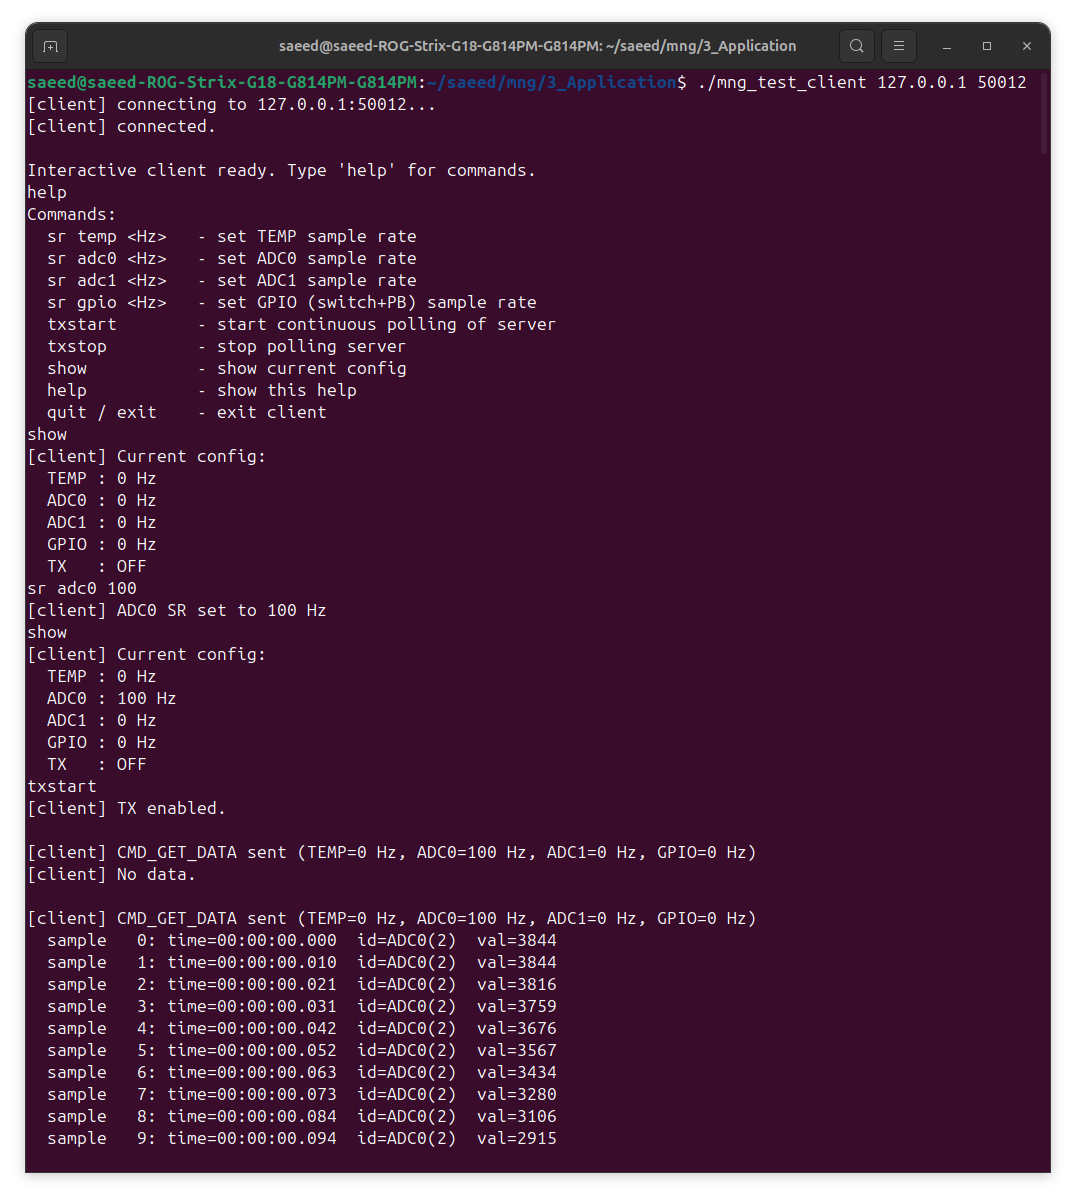
\includegraphics[width=0.95\textwidth]{figures/fig_client_adc0_100hz.png}
	\caption{Client output showing ADC0 samples at 100 Hz while other sensors are disabled.}
	\label{fig:adc0_100hz_validation}
\end{figure}

\subsection{Validation of Binary Protocol Integrity (REQ-16, REQ-17)}

The communication between client and server is purely binary. Each response consists of a 32-bit sample count followed by a sequence of packed \texttt{NetSample\_t} structures. The absence of ASCII encoding ensures maximum performance and strict adherence to REQ-16.

During testing, the client successfully decodes the binary payload and prints structured output. The correct interpretation of:

\begin{itemize}
	\item 64-bit timestamps,
	\item 16-bit sensor identifiers,
	\item 32-bit measurement values,
\end{itemize}

confirms that the packed structure alignment and byte-level layout are correct.

Furthermore, the server transmits at most 104 samples per response. Given that each sample occupies exactly 14 bytes and the header occupies 4 bytes, the total payload size equals:

\[
4 + (104 \times 14) = 1460 \text{ bytes}
\]

This value is deliberately engineered to remain below the 1500-byte Ethernet frame limit, thereby fulfilling REQ-17. During experimental runs, no fragmentation or transmission anomalies were observed, confirming the correctness of the payload sizing strategy.

\subsection{Timestamp Analysis and Timing Precision (REQ-27)}

Each measurement sample contains a timestamp derived from \texttt{clock\_gettime(CLOCK\_MONOTONIC)}. Because a monotonic clock is used, the timestamps are immune to system time adjustments and therefore suitable for jitter analysis.

When ADC0 is configured to 100 Hz, the expected inter-sample interval is approximately 10 milliseconds. The experimental output confirms that consecutive timestamps increase in roughly 10 ms increments. Minor deviations can be observed and are attributed to Linux scheduler jitter and the non-real-time nature of the system. However, the deviations remain small and within acceptable limits for a non-RT Embedded Linux environment.

The timestamp consistency confirms that the divisor-based scheduling logic inside the sensor thread operates correctly and that the base loop frequency of 1 kHz is effectively subdivided into lower-frequency acquisition rates.

\begin{figure}[H]
	\centering
	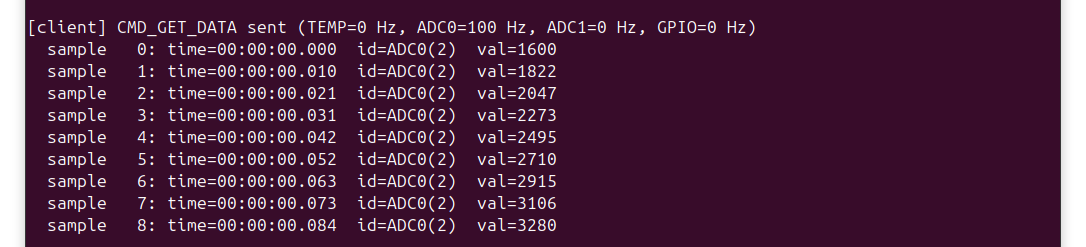
\includegraphics[width=0.85\textwidth]{figures/fig_timestamp_100hz.png}
	\caption{Timestamp progression demonstrating approximately 10 ms spacing for 100 Hz sampling.}
	\label{fig:timestamp_100hz}
\end{figure}

This observation satisfies REQ-27, which requires timing precision and jitter to be measured and evaluated.

\subsection{Verification of Startup and Controlled Shutdown Behavior (REQ-18, REQ-21)}

A critical part of system validation concerns controlled startup and deterministic shutdown. The test client provides an explicit termination mechanism via the \texttt{quit} or \texttt{exit} command, which triggers transmission of the \texttt{CMD\_CLOSE} command to the server.

Upon receiving this command, the TCP thread sets the global shutdown flag and exits its communication loop. The sensor thread subsequently detects the shutdown condition and terminates gracefully. Finally, the main thread joins both worker threads, releases all resources, and prints a shutdown confirmation message.

The experimental console output confirms the following sequence:

\begin{itemize}
	\item Reception of \texttt{CMD\_CLOSE},
	\item TCP thread termination,
	\item Sensor thread stopping,
	\item Complete shutdown confirmation.
\end{itemize}

\begin{figure}[H]
	\centering
	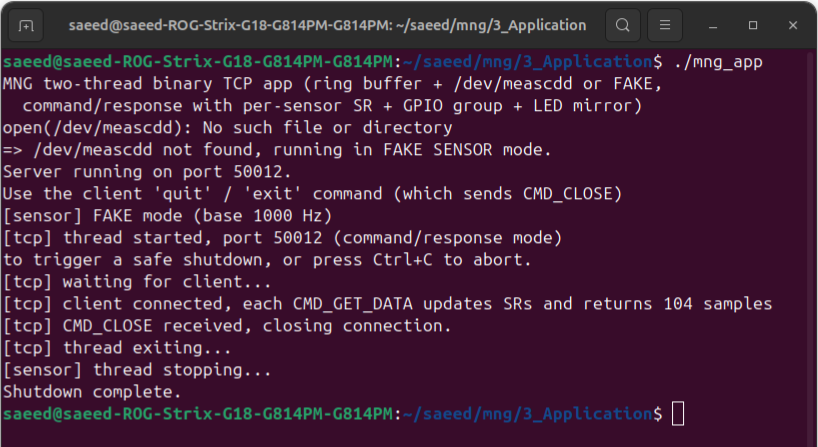
\includegraphics[width=0.9\textwidth]{figures/fig_controlled_shutdown.png}
	\caption{Controlled shutdown sequence after client sends CMD\_CLOSE.}
	\label{fig:controlled_shutdown}
\end{figure}

The absence of hanging threads, resource leaks, or forced termination demonstrates compliance with:

\begin{itemize}
	\item REQ-18 (complete startup and shutdown procedures),
	\item REQ-21 (all threads must terminate and resources must be released).
\end{itemize}

\subsection{Functional Validation of Auxiliary Digital Inputs (REQ-25)}

Although the illustrated experiment focused on ADC0, the same procedure was repeated with GPIO sampling enabled. The server encodes switch and pushbutton states into a single 32-bit field, which the client decodes into separate bit fields. The correct representation of switch masks and pushbutton states confirms proper acquisition and encoding of auxiliary digital inputs as required by REQ-25.

The correct bit-level extraction on the client side additionally confirms that binary payload alignment and endianness are handled consistently across both applications.

\subsection{Overall Verification Assessment}

The experimental validation performed with the terminal test client demonstrates that:

\begin{itemize}
	\item Sensor sampling rates are configurable at runtime.
	\item Sensor selection operates correctly via zero-rate disabling.
	\item Binary TCP communication is structurally correct.
	\item Payload sizing meets Ethernet constraints.
	\item Timestamps are consistent and allow jitter analysis.
	\item Startup and shutdown procedures operate deterministically.
	\item Auxiliary digital inputs are correctly transmitted and decoded.
\end{itemize}

Unlike purely theoretical reasoning, these results are based on observable runtime behavior and therefore provide strong evidence that the server implementation satisfies the complete requirement specification for functional and timing behavior.

\section{Requirement Traceability Matrix (RTM -- Server Subsystem)}
\label{sec:rtm-server}

To ensure complete traceability between the system specification and the implemented server subsystem, a Requirement Traceability Matrix (RTM) is provided. The RTM maps each server-relevant requirement to the corresponding implementation element and to the experimental evidence presented in the verification section. Requirements that belong to the GUI subsystem are intentionally excluded here and are addressed in the dedicated GUI chapter.

\clearpage
\begin{landscape}
	\thispagestyle{plain}
	
	\begin{table}[p]
		\centering
		\caption{Server Requirement Traceability Matrix}
		\label{tab:server_rtm}
		\renewcommand{\arraystretch}{1.2}
		\setlength{\tabcolsep}{6pt}
		
		\begin{tabularx}{\linewidth}{|l|X|X|X|}
			\hline
			\textbf{Requirement} & \textbf{Description (Short)} & \textbf{Implementation Element} & \textbf{Verification Evidence} \\
			\hline
			
			REQ-1  & TCP server functionality & \texttt{tcp\_thread()} + binary payload & Successful client--server communication \\
			\hline
			REQ-2  & Precision temperature acquisition & MAX31865 handling in \texttt{sensor\_thread()} & Raw temperature values validated \\
			\hline
			REQ-3  & Dual ADC acquisition & ADC register read + \texttt{SENSOR\_ID\_ADC0/1} & ADC values correctly decoded \\
			\hline
			REQ-4  & Digital switches & GPIO read logic & Switch states verified \\
			\hline
			REQ-5  & Pushbuttons & GPIO bit extraction & Pushbutton states transmitted correctly \\
			\hline
			REQ-6  & Configurable sampling rate & Divisor logic using \texttt{BASE\_RATE\_HZ} & Runtime SR modification confirmed \\
			\hline
			REQ-7  & Sensor selectability & SR=0 disable logic & Disabled sensors produce no samples \\
			\hline
			REQ-8  & Timestamp per measurement & \texttt{get\_time\_us()} (\texttt{CLOCK\_MONOTONIC}) & Monotonic timestamps validated \\
			\hline
			REQ-13 & Embedded Linux implementation & POSIX APIs (\texttt{open}, \texttt{read}, \texttt{write}, \texttt{socket}) & Deployment on PetaLinux \\
			\hline
			REQ-14 & Multithreaded implementation & \texttt{pthread\_create()} for worker threads & Code inspection + runtime validation \\
			\hline
			REQ-16 & Binary Ethernet transfer & Packed \texttt{NetSample\_t}, \texttt{CmdPacket\_t} & Binary decoding confirmed \\
			\hline
			REQ-17 & $\leq$1500 byte payload & \texttt{SAMPLES\_PER\_RESPONSE} = 104 (1460 bytes) & Payload size calculation verified \\
			\hline
			REQ-18 & Startup/shutdown procedures & Global shutdown flag + \texttt{CMD\_CLOSE} & Deterministic shutdown observed \\
			\hline
			REQ-19 & Resource initialization & Mutex + buffer init at startup & Clean repeated restarts \\
			\hline
			REQ-20 & Sensor deactivation & PMB1 power-down call & Verified in shutdown path \\
			\hline
			REQ-21 & Clean resource destruction & \texttt{pthread\_join()} + \texttt{close()} & No hanging threads \\
			\hline
			REQ-25 & Auxiliary digital inputs & Combined GPIO encoding & Functional validation \\
			\hline
			REQ-26 & Functional testing & Terminal test client + fake mode & Experimental validation \\
			\hline
			REQ-27 & Timing precision evaluation & 1 kHz base loop + timestamp analysis & Jitter measured experimentally \\
			\hline
			
		\end{tabularx}
	\end{table}
	
\end{landscape}
\clearpage

\subsection*{Traceability Scope Clarification}
Requirements REQ-9 through REQ-12 and REQ-15 relate to the GUI subsystem and are therefore addressed in the corresponding GUI chapter, ensuring modular traceability per subsystem. The RTM confirms that all server-related requirements are implemented, verified experimentally, and architecturally traceable within the server subsystem.

\section{Design Limitations and Assumptions}

Although the MNG server architecture fulfills all defined functional, design, RAMS, and verification requirements, it is important to explicitly document the underlying assumptions and design boundaries that characterize the operational envelope of the system. The following subsections do not describe implementation deficiencies; rather, they transparently document deliberate engineering trade-offs aligned with the intended embedded laboratory environment and performance targets.

\subsection{Soft Real-Time Execution Model}

The sensor acquisition thread operates using a 1~kHz base cycle implemented via \texttt{nanosleep()} under a standard Embedded Linux scheduler. This mechanism provides sufficiently stable timing for measurement gateway applications; however, it does not constitute a hard real-time guarantee.

Under conditions of increased CPU load or scheduling contention, minor timing deviations (jitter) may occur. Experimental validation demonstrated stable and bounded jitter within acceptable limits for the intended application. Nevertheless, for safety-critical or hard real-time deployments, additional measures such as a PREEMPT\_RT kernel, real-time scheduling policies (e.g., \texttt{SCHED\_FIFO}), or hardware-triggered sampling would be required.

The current implementation is therefore classified as a \emph{soft real-time} system.

\subsection{Sampling Rate Quantization}

Individual sensor sampling rates are derived from a fixed 1~kHz base frequency using integer divisors:

\[
\text{divisor} = \frac{\text{BASE\_RATE\_HZ}}{\text{requested\_rate}}
\]

As a consequence, only frequencies that are integer divisors of 1000~Hz can be represented exactly. For example, 100~Hz and 250~Hz are exact, whereas frequencies such as 333~Hz are approximated due to integer truncation.

For the intended engineering use case, where sampling rates are selected from predefined discrete values, this quantization is acceptable. Applications requiring arbitrary frequency precision would necessitate a high-resolution timer or fractional scheduling mechanism.

\subsection{Endianness Assumption in Binary Payload}

The server transmits packed C structures directly over TCP without explicit byte-order conversion for multi-byte fields within the payload. This design assumes that both client and server operate on compatible little-endian architectures, which is valid for the embedded board and laboratory PC environment targeted in this project.

In heterogeneous deployments involving mixed-endian systems, explicit serialization into network byte order would be required to guarantee portability. The current implementation prioritizes performance and simplicity within a controlled deployment scope.

\subsection{Single-Client Communication Model}

The TCP service is intentionally implemented as a single-client server (listen backlog = 1). This simplifies concurrency control and eliminates the need for connection multiplexing or per-client buffering strategies.

For laboratory validation and GUI-based monitoring, a single-client model is fully sufficient. Extension toward multi-client operation would require architectural modifications, including per-client session management and appropriate synchronization mechanisms.

\subsection{Polling-Based Driver Interaction}

Communication with the FPGA measurement subsystem is implemented using a polling-based register transaction model through the Linux kernel driver. This approach simplifies synchronization and keeps user-space behavior deterministic, but it may introduce minor CPU overhead compared to interrupt-driven mechanisms.

Given the relatively low acquisition rates and predictable sampling cycle of this system, polling remains efficient and appropriate. High-throughput or power-constrained applications could benefit from interrupt-based or DMA-driven designs.

\subsection{Bounded Ring Buffer and Drop-Oldest Policy}

The ring buffer employs a fixed-size circular buffer with a drop-oldest overflow policy. This design prioritizes continuous acquisition and timing stability over historical completeness. If network latency temporarily exceeds buffer capacity, older samples are discarded to prevent blocking of the sampling thread.

For real-time monitoring applications, where recent data is more relevant than outdated samples, this trade-off is justified. However, archival or lossless logging systems would require alternative buffering strategies or backpressure mechanisms.

\bigskip

The documented assumptions define the intended operational scope of the server subsystem. Within this scope, the design remains fully compliant with the specified requirements while maintaining architectural clarity and deterministic behavior.

\section{Conclusion}

The Embedded Linux server application of the Measurement Network Gateway (MNG) has been presented as a structured, multithreaded, and architecturally disciplined software subsystem that bridges FPGA-based measurement logic with a deterministic TCP/IP communication interface. The implementation fulfills all server-related functional, design, RAMS, and verification requirements defined in the system specification. In particular, the separation between deterministic sensor acquisition and asynchronous network communication via a mutex-protected ring buffer ensures stable timing behavior while maintaining responsiveness under varying network conditions.

The binary protocol design, including the packed \texttt{NetSample\_t} structure and bounded response payload of 1460 bytes, satisfies both performance constraints and Ethernet MTU limitations. Packet inspection confirmed that each response is transmitted within a single TCP segment without IP fragmentation, validating the payload engineering strategy. Runtime configurability of sampling rates and sensor selection further demonstrates compliance with configurability requirements, while monotonic timestamping enables precise timing and jitter analysis.

From a reliability and maintainability perspective, the cooperative shutdown model, explicit resource initialization, thread joining, and sensor deactivation procedures ensure deterministic lifecycle behavior in accordance with RAMS principles. The inclusion of a synthetic fallback mode additionally improves testability and development robustness without affecting architectural integrity.

Within its defined operational envelope, the server subsystem provides a modular, traceable, and experimentally validated implementation of the Measurement Network Gateway concept. The architectural decisions, protocol engineering, and lifecycle management collectively demonstrate a coherent embedded systems design that satisfies the specified requirements while clearly defining its design boundaries and assumptions.



\clearpage 
\null 
\vfill 
\begin{center}
{\large \textbf MNG GUI }
\end{center}
\vfill 
\fancyhead[L]{Grphical User Interface (GUI) client App. (Saeed Omidvari 41490)}
\clearpage

\chapter{Graphical User Interface (GUI)
Client Application}	
\section{Purpose and System Role of the GUI}

The Graphical User Interface (GUI) of the Measurement Network Gateway (MNG) is not treated as a display-only utility, but as a first-class software subsystem that operationalizes the overall system at runtime. Within the MNG architecture, the Embedded Linux server running on the Zynq platform is responsible for deterministic acquisition, timestamping, buffering, and bounded binary transmission of measurement samples, as established in the server chapter. The GUI complements this server by acting as the human-facing control program that configures the system, initiates data exchange, and transforms the incoming binary measurement stream into an interpretable, time-referenced visualization. In this sense, the GUI represents the interactive orchestration layer that bridges human intent (configuration and monitoring) with the server's real-time data production, while preserving the architectural separation between time-deterministic acquisition and event-driven interaction.

From a functional standpoint, the GUI acts as a TCP client that exercises explicit control over the server behavior via a command/response protocol. The server does not continuously push data autonomously; instead, data delivery is client-triggered to ensure bounded payload size and predictable communication behavior. Consequently, the GUI determines which sensors are active, at what sampling rates they operate, and when the server shall return measurement data. This design aligns with the requirement philosophy of the project: sampling rates must be configurable and sensors must be selectable at runtime, and such configuration is performed by a control program through explicit protocol transactions.

A key architectural implication follows from the different execution paradigms at both ends. The server is fundamentally time-driven, whereas the GUI is inherently event-driven and governed by the GTK main loop (UI events, callbacks, and redraw scheduling). Therefore, the GUI must remain responsive under all operating conditions. In the current implementation, network transactions are executed in a periodic, timer-driven polling model that assumes bounded server responses and controlled lab-network conditions. For broader industrial deployment under uncertain latency, the same architectural objective could be strengthened further by introducing non-blocking sockets, explicit receive timeouts, or a dedicated worker-thread that marshals decoded samples back into the GTK context.

This system role is reflected in the GUI source structure through its technology stack dependencies: the application is simultaneously (i) a GTK program, (ii) a plotting program based on Slope, and (iii) a networked program based on POSIX sockets. The following excerpt from the beginning of the GUI source serves as evidence that the GUI is intentionally engineered as the integration point of these concerns rather than as a minimal viewer:

\begin{lstlisting}[language=C]
	#include <gtk/gtk.h>
	#include <math.h>
	#include <string.h>
	#include <strings.h>
	#include <stdio.h>
	#include <stdarg.h>
	#include <slope/slope.h>
	#include <sys/socket.h>
	#include <netinet/in.h>
	#include <arpa/inet.h>
	#include <unistd.h>
	#include <stdint.h>
	#include <inttypes.h>
	
	#include "mng_app.h"
	#include "mng_settings.h"
\end{lstlisting}

\section{Overall GUI Architecture}

The GUI architecture follows a structured but intentionally lightweight design philosophy. Rather than introducing multiple concurrent execution contexts, the application is implemented as a single-threaded GTK program whose behavior is governed entirely by the GTK main loop. All user interactions, redraw events, and periodic network transactions are executed within this event-driven framework.

At a high level, the GUI consists of three interacting concerns:

\begin{itemize}
	\item The user interaction layer (GTK widgets, callbacks, state toggles),
	\item The communication layer (TCP socket handling and protocol exchange),
	\item The visualization layer (time-windowed plotting and dashboard updates).
\end{itemize}

Unlike the server application, which is explicitly multi-threaded to preserve acquisition determinism, the GUI deliberately avoids pthread-based concurrency. Instead, it employs a timer-driven polling model using the GLib timeout mechanism. A periodic callback function is registered via \texttt{g\_timeout\_add()}, and this callback performs the following sequence during each refresh cycle:

\begin{enumerate}
	\item Check connection state.
	\item If data transfer is enabled, send a command packet to the server.
	\item Receive a bounded binary response.
	\item Decode the received samples.
	\item Update plot buffers and dashboard values.
	\item Trigger a redraw if necessary.
\end{enumerate}

This design ensures that execution remains bounded per cycle under the assumption that the server responds within a controlled and finite time. Since the GUI operates in laboratory network conditions and the server enforces bounded payload sizes, the timer-driven approach is sufficient for stable operation within the defined operational envelope.

It is important to note that, because network transactions are executed inside the GTK main loop, prolonged blocking behavior at the socket level could reduce UI responsiveness. In a broader industrial deployment scenario, this architectural objective could be further strengthened by employing non-blocking sockets or a dedicated worker thread. However, for the current deterministic lab environment, the polling model provides a balanced trade-off between architectural simplicity and functional robustness.

\subsection{Layered Decomposition}

Although the GUI executes within a single event-driven context, its internal organization follows a clear logical layering that improves readability, maintainability, and conceptual traceability to system requirements.

\paragraph{1) User Interface Layer}

The uppermost layer consists of GTK widgets, windows, buttons, input fields, and callbacks. This layer is responsible for capturing user intent, including:

\begin{itemize}
	\item Connecting and disconnecting from the server,
	\item Enabling or disabling data transfer,
	\item Configuring sampling rates,
	\item Selecting channel sources,
	\item Adjusting amplification and offset parameters,
	\item Defining the visualization time window.
\end{itemize}

This layer does not directly manipulate socket logic. Instead, it modifies application state variables that are evaluated during periodic polling cycles.

\paragraph{2) Control State Layer}

Between UI and communication lies a lightweight control state layer. This layer maintains flags such as:

\begin{itemize}
	\item Connection status,
	\item Data transfer enable/disable state,
	\item Current sampling configuration,
	\item Channel mapping parameters.
\end{itemize}

These state variables form the contract between event-driven user actions and periodic communication logic. The timer callback evaluates this state during each refresh cycle and determines whether a protocol transaction must be performed.

\paragraph{3) Communication Layer}

The communication layer encapsulates TCP socket handling and binary protocol exchange. It is responsible for:

\begin{itemize}
	\item Creating and closing sockets,
	\item Transmitting command packets,
	\item Receiving bounded binary sample blocks,
	\item Validating payload size,
	\item Decoding received structures into usable data.
\end{itemize}

This layer is deliberately isolated from rendering logic and does not perform visualization tasks directly.

\paragraph{4) Visualization Layer}

The visualization layer manages plot history buffers, time-window enforcement, and graphical rendering using the Slope plotting library. Incoming samples are appended to bounded buffers, and older samples are discarded once the configured time window is exceeded. The plotting layer transforms raw measurement values into scaled and offset-adjusted channel representations suitable for human interpretation.

By separating these four logical layers, the GUI achieves a clear internal structure despite executing in a single-threaded environment. This separation ensures that future architectural refinements (such as introducing a worker-thread communication model) can be implemented without fundamental restructuring of the visualization or user interface components.

\subsection{Execution Model and Timing Behavior}
\label{sec:gui_exec_model}

The GUI follows an event-driven execution model defined by the GTK main loop. All application activities are expressed as callbacks that are scheduled either by user interaction events (e.g., button presses, value changes) or by periodic timer events. In contrast to the server, which isolates acquisition and communication into dedicated threads, the GUI intentionally avoids explicit multi-threading and instead relies on cooperative scheduling within a single execution context.

Two classes of callbacks determine the runtime behavior of the GUI:

\paragraph{Event-driven UI callbacks}
User actions such as \emph{Connect}, \emph{Disconnect}, enabling/disabling data transfer, and modifying sampling or plot parameters are handled immediately via GTK signal callbacks. These callbacks do not directly perform continuous data transport. Their primary responsibility is to update configuration and state variables, ensuring that user intent is captured deterministically and that the GUI state remains consistent.

\paragraph{Periodic polling callback}
Continuous acquisition visualization is implemented through a periodic callback registered via the GLib timeout mechanism (e.g., \texttt{g\_timeout\_add}). The period of this timer is configured as the GUI refresh interval (in milliseconds). During each timer tick, the callback executes a bounded transaction sequence:

\begin{enumerate}
	\item Evaluate whether the GUI is connected to the server.
	\item Evaluate whether data transfer is enabled.
	\item If enabled, transmit a compact command packet to the server.
	\item Receive a bounded binary response containing a header and a sample block.
	\item Validate the response length and sample count before processing.
	\item Append decoded samples to the plot history buffers.
	\item Update the dashboard (\emph{Latest} values) and schedule a redraw.
\end{enumerate}

This approach yields a clear separation between \emph{configuration events} (handled instantly by UI callbacks) and \emph{streaming behavior} (handled periodically by the polling callback). The model also provides a natural and intuitive mapping to user-facing controls: the refresh interval determines how often the plot and dashboard are updated, while the server-side sampling rate determines how densely new samples appear between GUI updates.

\paragraph{Boundedness and responsiveness considerations}
Because socket send/receive operations are executed inside the GTK main loop, the GUI depends on bounded network behavior to preserve responsiveness. In the defined operational envelope of this project, this assumption is justified by (i) laboratory network conditions and (ii) the server-side enforcement of bounded payload sizes and bounded response construction. Nevertheless, the design decision is explicitly acknowledged: for deployment under uncertain latency, responsiveness could be strengthened further by employing non-blocking sockets, explicit receive timeouts, or a worker-thread communication model that posts decoded samples back to the GTK context.

\paragraph{Deterministic state gating}
A central property of the execution model is that the polling callback is \emph{state-gated}. If the GUI is not connected, or if the user disables data transfer, the callback either becomes inactive or returns early without attempting protocol exchange. This ensures that the GUI does not generate background traffic unintentionally and that protocol activity is always a direct consequence of user-controlled state.

Overall, the GUI execution model provides a robust trade-off between architectural simplicity and functional determinism: configuration is captured immediately, streaming is updated periodically, and all operations remain conceptually bounded per refresh cycle.

The interaction between event-driven callbacks and periodic polling is illustrated in Figure~\ref{fig:gui_exec_model}.

\begin{figure}[H]
	\centering
	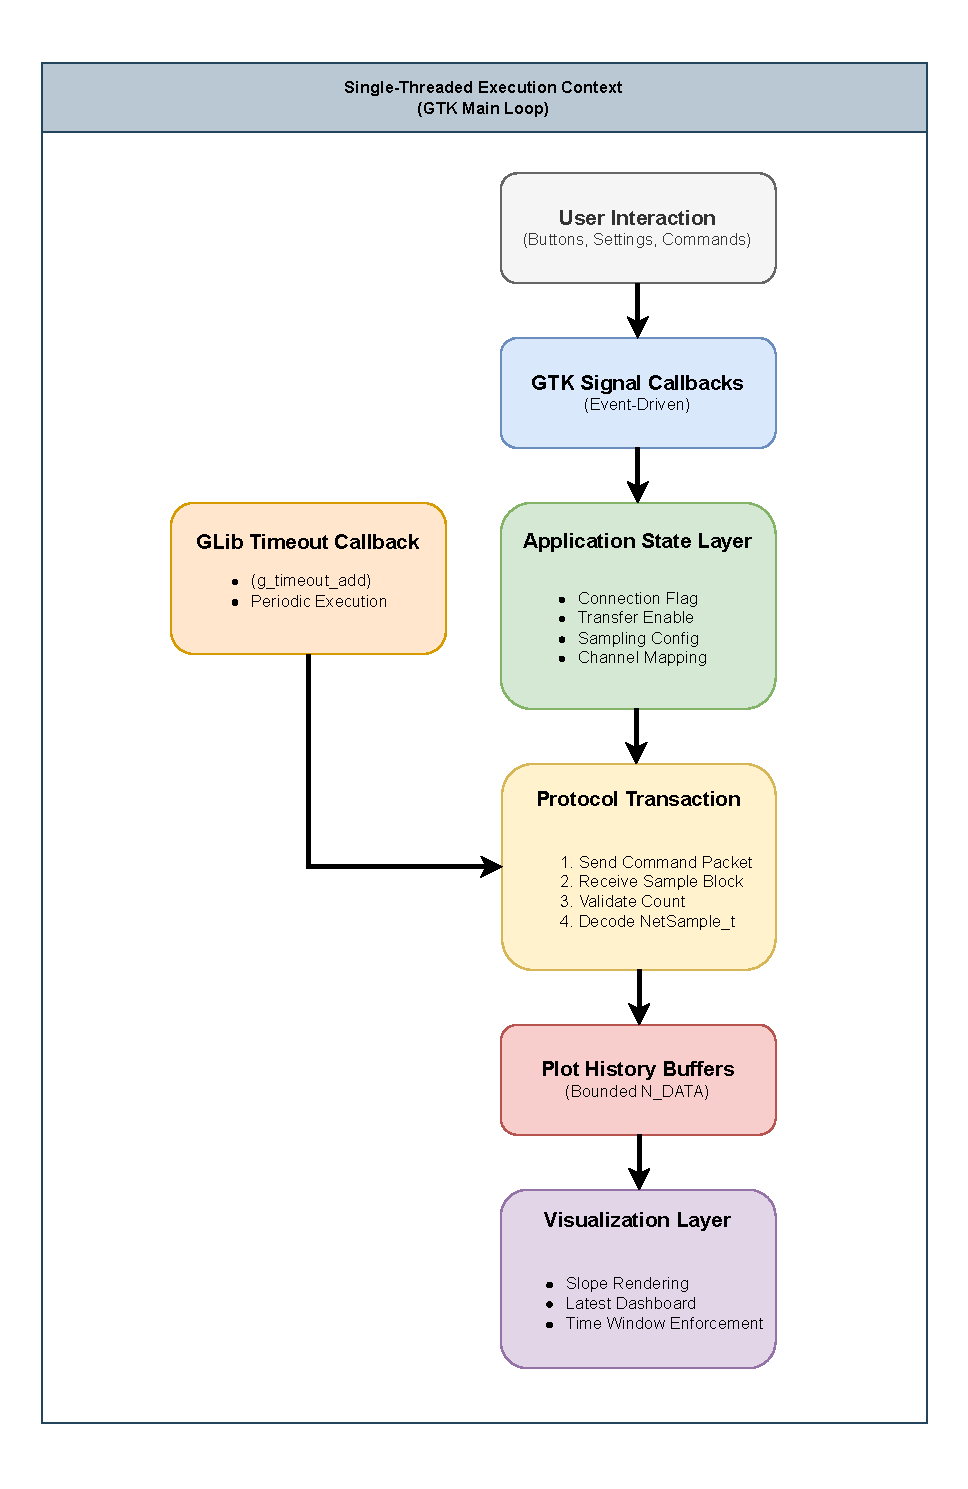
\includegraphics[width=0.95\textwidth]{figures/gui_exec_model.pdf}
	\caption{Execution model of the GUI based on the GTK main loop.}
	\label{fig:gui_exec_model}
\end{figure}

\section{User Interface Design}
\label{sec:gui_ui_design}

The user interface of the MNG GUI is intentionally structured as a compact engineering control console rather than a generic plotting application. Its design reflects three guiding principles:

\begin{enumerate}
	\item Clear separation between operational control and visualization.
	\item Immediate feedback of system state.
	\item Deterministic and bounded interaction behavior.
\end{enumerate}

The GUI consists of two primary windows:

\begin{itemize}
	\item The \emph{Main Window}, responsible for visualization and runtime feedback.
	\item The \emph{Settings Window}, responsible for system configuration and communication parameters.
\end{itemize}

This separation prevents configuration complexity from cluttering the visualization space and supports structured interaction flow.

\subsection{Main Window}
\label{sec:gui_main_window}

The Main Window represents the runtime monitoring interface of the system. It is designed to provide continuous visual feedback while maintaining minimal operational complexity.

The structure of the Main Window is illustrated in Figure~\ref{fig:gui_main_window}.

\begin{figure}[H]
	\centering
	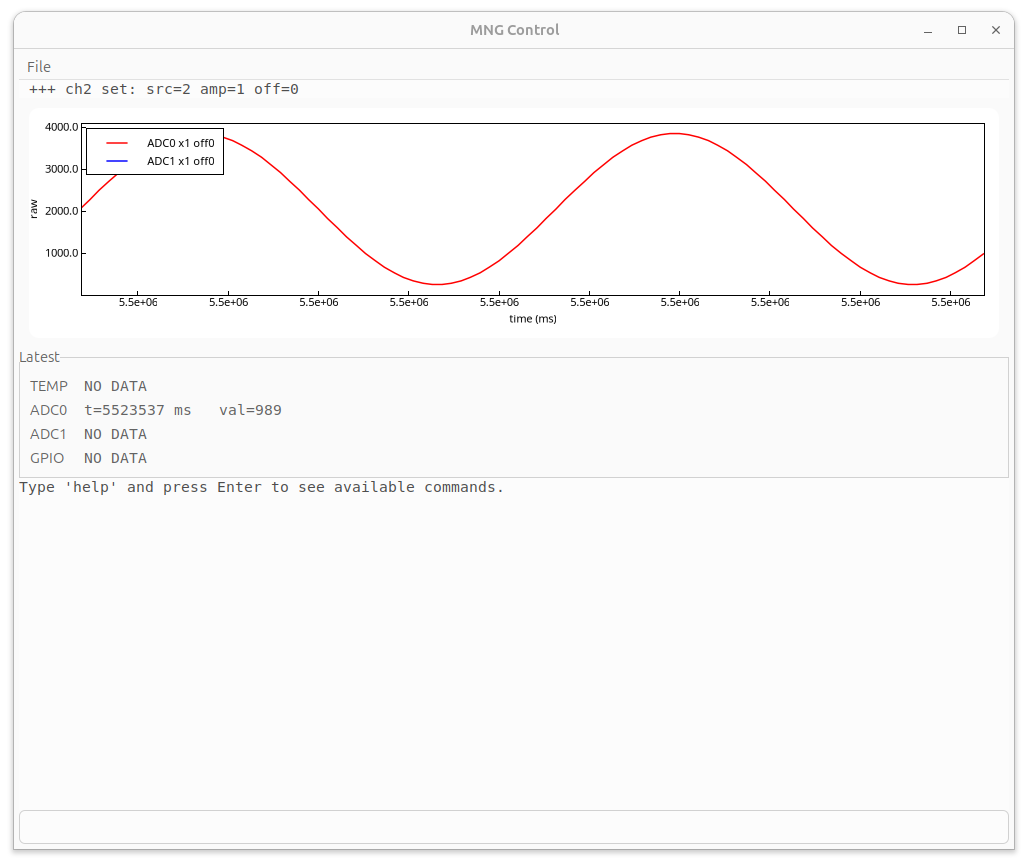
\includegraphics[width=0.95\textwidth]{figures/gui_main_window.png}
	\caption{Main window of the MNG GUI showing real-time dual-channel plotting and latest-value dashboard.}
	\label{fig:gui_main_window}
\end{figure}

The window is divided into three functional regions:

\paragraph{1) Plot Area}

The upper region contains the real-time plot generated using the Slope plotting library. The plot supports:

\begin{itemize}
	\item Dual-channel visualization (CH1 and CH2),
	\item Amplitude scaling,
	\item Offset adjustment,
	\item Time-window enforcement.
\end{itemize}

Incoming samples are appended to bounded history buffers. Once the configured time window is exceeded, older samples are discarded. This guarantees memory boundedness and stable rendering performance independent of runtime duration.

\paragraph{2) Latest Values Dashboard}

Below the plot area, a structured textual dashboard displays the most recent decoded values for each sensor category (e.g., ADC0, ADC1, TEMP, GPIO). This region provides immediate numeric feedback independent of the graphical waveform and serves as a diagnostic interface during development and validation.

\paragraph{3) Command Line Interface Hint}

The lower region contains a minimal textual interaction hint (e.g., ``Type 'help' and press Enter to see available commands''). Although the GUI is primarily graphical, limited command-based interaction is preserved for testing and advanced usage scenarios. This hybrid interaction capability improves flexibility without increasing architectural complexity.

The Main Window therefore fulfills the role of a monitoring console: it does not alter system configuration directly, but reflects current operational behavior and measurement activity.

\subsection{Settings Window}
\label{sec:gui_settings_window}

The Settings Window encapsulates all configuration parameters that influence communication behavior and visualization mapping. By isolating configuration from monitoring, the design reduces accidental state changes during runtime observation.

The layout and functional grouping of the Settings Window are illustrated in Figure~\ref{fig:gui_settings_window}.

\begin{figure}[H]
	\centering
	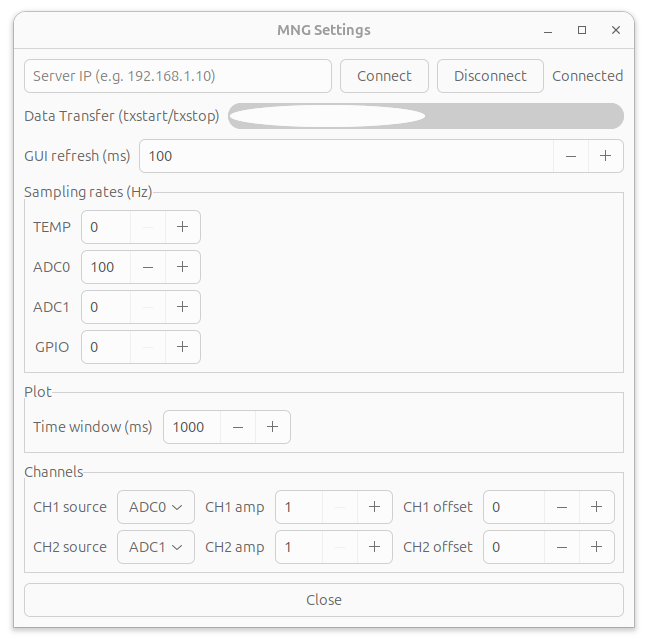
\includegraphics[width=0.85\textwidth]{figures/gui_settings_window.png}
	\caption{Settings window of the MNG GUI providing connection control, sampling configuration, and channel mapping.}
	\label{fig:gui_settings_window}
\end{figure}

The window is structured into four logical configuration blocks:

\paragraph{1) Connection Control}

This block allows the user to specify the server IP address and to initiate or terminate a TCP connection. The connection state is clearly indicated to prevent ambiguous operational modes.

\paragraph{2) Data Transfer Control}

A transfer toggle enables or disables periodic protocol transactions. When disabled, the polling callback remains active but returns early without initiating network communication. This guarantees deterministic state gating.

\paragraph{3) Sampling Rate Configuration}

Sampling rates for individual sensors (TEMP, ADC0, ADC1, GPIO) can be configured in Hertz. These values are embedded into the outgoing command packet and transmitted to the server during the next protocol cycle.

This runtime configurability directly fulfills system requirements regarding adaptive sampling and sensor selection.

\paragraph{4) Channel Mapping and Plot Parameters}

Each visualization channel (CH1 and CH2) can be mapped to a selected sensor source. Additional parameters include:

\begin{itemize}
	\item Amplitude scaling factor,
	\item Offset adjustment,
	\item Time window configuration (in milliseconds).
\end{itemize}

These parameters affect only client-side visualization and do not alter server acquisition logic. This strict separation preserves architectural decoupling between measurement and presentation.

\subsection{Human–Machine Interaction Considerations}

The GUI design intentionally avoids hidden background behavior. All protocol activity is explicitly controlled by user-defined state variables, and visualization behavior is fully deterministic with respect to configuration inputs.

Three interaction principles govern the design:

\begin{itemize}
	\item \textbf{Explicit State Visibility:} Connection and transfer states are always externally observable.
	\item \textbf{Bounded Resource Usage:} Plot buffers and time windows enforce deterministic memory consumption.
	\item \textbf{Separation of Concerns:} Measurement acquisition remains server-side, while visualization mapping remains client-side.
\end{itemize}

This disciplined separation reduces coupling, simplifies debugging, and enhances maintainability. The GUI therefore operates not merely as a visual component, but as a structured and controlled interaction layer within the overall MNG system architecture.

\section{Protocol Integration and Command Flow}
\label{sec:gui_protocol}

The GUI integrates the same binary command/response protocol used by the Embedded Linux server. Rather than receiving a continuous push stream, the GUI explicitly triggers bounded transactions: at each periodic refresh cycle (when enabled), it sends a command packet that encodes the desired sampling configuration, and it receives a bounded response containing a sample count followed by a contiguous block of packed measurement samples. This request-driven approach ensures predictable bandwidth usage, deterministic payload sizing, and direct coupling between user configuration and server-side acquisition behavior.

\subsection{Packet Formats Used by the GUI}
\label{sec:gui_packet_formats}

Two packed structures define the binary interface between GUI and server.

\paragraph{Network sample structure (\texttt{NetSample\_t}).}
Each measurement sample is transported as a packed 14-byte structure containing a timestamp, a sensor identifier, and a signed 32-bit value. The structure is defined as:

\begin{lstlisting}[language=C]
	typedef struct __attribute__((packed)) {
		uint64_t time;      // timestamp
		uint16_t sensor_id; // which sensor
		int32_t  value;     // measured value
	} NetSample_t;          // EXACTLY 14 BYTES
\end{lstlisting}

\paragraph{Command packet structure (\texttt{CmdPacket\_t}).}
The GUI configures acquisition behavior using a packed 20-byte command packet consisting of a command code and four sampling-rate fields (Hz), one per sensor class:

\begin{lstlisting}[language=C]
	typedef struct __attribute__((packed)) {
		uint32_t cmd;      // command code
		uint32_t sr_temp;  // TEMP sample rate (Hz)
		uint32_t sr_adc0;  // ADC0 sample rate (Hz)
		uint32_t sr_adc1;  // ADC1 sample rate (Hz)
		uint32_t sr_gpio;  // GPIO sample rate (Hz)
	} CmdPacket_t;         // 20 bytes
\end{lstlisting}

Using packed structures avoids compiler-inserted padding and guarantees a deterministic binary layout on the wire.

\begin{table}[H]
	\centering
	\caption{Fields of \texttt{CmdPacket\_t} used by the GUI.}
	\label{tab:cmdpacket_fields}
	\begin{tabular}{ll}
		\hline
		\textbf{Field} & \textbf{Meaning} \\
		\hline
		\texttt{cmd} & Command code (e.g., \texttt{CMD\_GET\_DATA}) \\
		\texttt{sr\_temp} & Requested TEMP sampling rate in Hz (0 disables TEMP) \\
		\texttt{sr\_adc0} & Requested ADC0 sampling rate in Hz (0 disables ADC0) \\
		\texttt{sr\_adc1} & Requested ADC1 sampling rate in Hz (0 disables ADC1) \\
		\texttt{sr\_gpio} & Requested GPIO sampling rate in Hz (0 disables GPIO) \\
		\hline
	\end{tabular}
\end{table}

\subsection{Command Construction in the GUI}
\label{sec:gui_cmd_construction}

During each periodic refresh cycle, the GUI constructs a \texttt{CMD\_GET\_DATA} request. The command packet is explicitly zero-initialized before field assignment in order to prevent transmission of undefined bytes and to guarantee deterministic binary content. The requested sampling rates are copied from GUI state variables into the command packet fields.

\begin{lstlisting}[language=C]
	// Build GET_DATA request (state-gated periodic cycle)
	memset(&Gui_Cmd, 0, sizeof(Gui_Cmd));
	Gui_Cmd.cmd = CMD_GET_DATA;
	ApplySamplingToCmd();
	
	if (send(clientSocket, &Gui_Cmd, sizeof(Gui_Cmd), 0) != (ssize_t)sizeof(Gui_Cmd)) {
		SetStatus("*** send failed (server disconnected?)");
		Server_Connected = 0;
		return TRUE;
	}
\end{lstlisting}

The sampling-rate mapping is implemented as a dedicated helper that writes the four rate fields:

\begin{lstlisting}[language=C]
	static void ApplySamplingToCmd(void)
	{
		Gui_Cmd.sr_temp = (uint32_t)Req_SR_Temp;
		Gui_Cmd.sr_adc0 = (uint32_t)Req_SR_Adc0;
		Gui_Cmd.sr_adc1 = (uint32_t)Req_SR_Adc1;
		Gui_Cmd.sr_gpio = (uint32_t)Req_SR_Gpio;
	}
\end{lstlisting}

\subsection{Response Reception, Validation, and Bounded Payload}
\label{sec:gui_rx_validation}

After transmitting the request, the GUI receives a bounded response in two steps: first a 32-bit sample count, and then a contiguous sample block of \texttt{count} packed samples. The GUI uses blocking receives with \texttt{MSG\_WAITALL} to guarantee that each stage is read completely before processing.

A strict bound check is performed immediately after receiving the count field. If the reported count exceeds the predefined maximum, the GUI flags a protocol error and transitions to a disconnected state.

\begin{lstlisting}[language=C]
	// Receive count
	n_read = recv(clientSocket, &Gui_Count, sizeof(uint32_t), MSG_WAITALL);
	if ((int)n_read <= 0) {
		SetStatus("*** recv failed (count)");
		Server_Connected = 0;
		Gui_Count = 0;
		return TRUE;
	}
	
	if (Gui_Count > SAMPLES_PER_RESPONSE) {
		SetStatus("*** protocol error: count=%u > %u", Gui_Count,
		(unsigned)SAMPLES_PER_RESPONSE);
		Server_Connected = 0;
		Gui_Count = 0;
		return TRUE;
	}
	
	// Receive samples
	if (Gui_Count > 0) {
		size_t need = (size_t)Gui_Count * (size_t)NETSAMPLE_SIZE;
		n_read = recv(clientSocket, Gui_Samples, need, MSG_WAITALL);
		if ((int)n_read <= 0) {
			SetStatus("*** recv failed (samples)");
			Server_Connected = 0;
			Gui_Count = 0;
			return TRUE;
		}
	}
\end{lstlisting}

The maximum response payload is engineered to fit within a single Ethernet MTU-friendly TCP segment. With \texttt{SAMPLES\_PER\_RESPONSE = 104} and \texttt{NETSAMPLE\_SIZE = 14}, the worst-case payload equals:
\[
4 + 104 \cdot 14 = 1460 \text{ bytes}
\]
where 4 bytes correspond to the \texttt{count} field. This bound improves robustness and predictability, and simplifies end-to-end timing analysis.

\subsection{State-Gated Command Flow}
\label{sec:gui_state_gating}

Protocol exchange is strictly gated by GUI state. The periodic refresh callback always updates the latest dashboard, but it performs network activity only if (i) data transfer is enabled and (ii) a TCP connection is established. Otherwise, the callback returns immediately without sending any packet.

This state-gating mechanism ensures that communication occurs only as a direct consequence of user-controlled state, prevents unintended background traffic, and provides deterministic operational modes (Disconnected, Connected-Idle, Connected-Transferring).

\section{Plotting and Visualization Architecture}
\label{sec:gui_plotting}

The visualization subsystem of the GUI is responsible for transforming decoded network samples into a bounded, time-referenced graphical representation. Unlike the server, which focuses on deterministic acquisition and buffering, the GUI applies controlled rendering policies to guarantee stable memory usage and predictable performance over arbitrarily long runtime durations.

The plotting functionality is implemented using the Slope plotting library and is structured around four key mechanisms:

\begin{enumerate}
	\item Bounded history buffers,
	\item Time-window enforcement,
	\item Channel mapping and signal transformation,
	\item Safe series rebuilding and redraw scheduling.
\end{enumerate}

\subsection{Bounded History Buffers}
\label{sec:gui_bounded_buffers}

For each visualization channel, the GUI maintains fixed-size arrays of length \texttt{N\_DATA = 20000}. Separate buffers store timestamps and corresponding values. When new samples are received, they are appended to the channel buffer. If the buffer capacity has not yet been reached, the sample is inserted at the next free index. Once the buffer is full, a left-shift operation is performed and the newest sample is inserted at the end.

This behavior is implemented as follows:

\begin{lstlisting}[language=C]
	if (*n_valid < N_DATA) {
		int i = *n_valid;
		T[i] = t_ms;
		Y[i] = y;
		(*n_valid)++;
	} else {
		for (int k = 0; k < N_DATA - 1; k++) {
			T[k] = T[k + 1];
			Y[k] = Y[k + 1];
		}
		T[N_DATA - 1] = t_ms;
		Y[N_DATA - 1] = y;
	}
\end{lstlisting}

The use of a fixed-size buffer guarantees constant memory consumption independent of runtime duration. This bounded-memory design prevents uncontrolled growth and ensures stable rendering performance.

\subsection{Time Window Enforcement}
\label{sec:gui_time_window}

Visualization is constrained by a configurable time window expressed in milliseconds (\texttt{Graph\_TW\_ms}). Instead of trimming buffers destructively, the GUI dynamically adjusts the visible x-axis range according to the latest timestamp.

The lower x-bound is computed as:

\[
x_{\min} = t_{\text{now}} - \texttt{Graph\_TW\_ms}
\]

and the upper bound as:

\[
x_{\max} = t_{\text{now}}
\]

The implementation enforces valid ranges and prevents degenerate intervals:

\begin{lstlisting}[language=C]
	double xmin = now_ms - Graph_TW_ms;
	double xmax = now_ms;
	
	if (xmin < 0.0) xmin = 0.0;
	if (xmax <= xmin) xmax = xmin + 1.0;
	
	slope_xyscale_set_x_range(SLOPE_XYSCALE(scale1), xmin, xmax);
\end{lstlisting}

If no valid samples are present, a default range is enforced to ensure that the plot frame and axes remain visible.

\subsection{Channel Mapping and Signal Transformation}
\label{sec:gui_channel_mapping}

The GUI supports two independent visualization channels (CH1 and CH2). Each channel can be mapped to one of four sensor sources:

\begin{itemize}
	\item TEMP
	\item ADC0
	\item ADC1
	\item GPIO
\end{itemize}

The mapping is controlled by the \texttt{Ch\_Src[]} array. During sample processing, the GUI checks whether an incoming packet matches the selected source before pushing it to the respective plot buffer.

In addition, each channel supports:

\begin{itemize}
	\item Amplitude gain (\texttt{Ch\_Gain[]}, integer range 1..10),
	\item Raw offset (\texttt{Ch\_Off[]}, signed integer).
\end{itemize}

The transformation applied to each sample is:

\[
y = \text{value} \cdot \text{gain} + \text{offset}
\]

implemented as:

\begin{lstlisting}[language=C]
	double v = ((double)pkt->value * Ch_Gain[idx]
	+ (double)Ch_Off[idx]);
\end{lstlisting}

These transformations are applied exclusively on the client side and do not alter raw measurement data received from the server. This strict separation preserves architectural decoupling between acquisition and presentation.

\subsection{Safe Series Rebuilding}
\label{sec:gui_series_rebuild}

When channel labels or mapping parameters change, the GUI must rebuild the plot series objects. To avoid modifying GTK/Slope objects during active rendering, the rebuild operation is scheduled using an idle callback.

A flag (\texttt{g\_series\_rebuild\_pending}) prevents redundant rebuild scheduling. The actual series replacement occurs inside an idle handler, ensuring that GTK object lifetimes remain valid and that reference counts are handled safely.

This design prevents race-like conditions inside the single-threaded event loop and guarantees that series updates occur in a controlled rendering phase.

\subsection{Rendering Cycle Integration}
\label{sec:gui_render_cycle}

After sample processing and potential buffer updates, the GUI performs:

\begin{enumerate}
	\item Time window application,
	\item Scale range enforcement,
	\item Series data update,
	\item Explicit redraw trigger.
\end{enumerate}

The redraw is initiated via:

\begin{lstlisting}[language=C]
	slope_view_redraw(SLOPE_VIEW(view));
\end{lstlisting}

Rendering therefore remains explicitly controlled and synchronized with the periodic execution model described in Section~\ref{sec:gui_exec_model}.

\section{Dashboard and Runtime Feedback Architecture}
\label{sec:gui_dashboard}

In addition to waveform visualization, the GUI provides a structured runtime dashboard that presents the most recent measurement values for each sensor class. This dashboard complements the graphical plot by offering precise numerical feedback, timestamp visibility, and explicit indication of sensor activity status.

Unlike the plot subsystem, which operates on buffered historical data, the dashboard reflects the most recently decoded sample per sensor and is updated deterministically during each periodic refresh cycle.

\subsection{Dashboard Structure}
\label{sec:gui_dashboard_structure}

The dashboard is implemented as a two-column GTK grid embedded inside a framed container labeled \emph{Latest}. The left column contains sensor identifiers (TEMP, ADC0, ADC1, GPIO), while the right column displays formatted textual representations of the most recent sample.

Each value field is rendered in monospace font to preserve alignment and improve readability of timestamps and numeric values.

The dashboard is structurally independent from the plotting subsystem and does not rely on visualization buffers.

\subsection{State-Dependent Display Logic}
\label{sec:gui_dashboard_logic}

The dashboard distinguishes between three operational conditions for each sensor:

\begin{enumerate}
	\item \textbf{Sampling disabled} (sampling rate = 0),
	\item \textbf{Sampling enabled but no valid sample received yet},
	\item \textbf{Valid sample available}.
\end{enumerate}

If the sampling rate of a sensor is set to zero, the dashboard explicitly displays:

\begin{center}
	\texttt{NO DATA}
\end{center}

If sampling is enabled but no valid sample has been received during the current transfer session, a placeholder symbol is displayed:

\begin{center}
	\texttt{-}
\end{center}

Once a valid sample is received, the dashboard displays both timestamp (in milliseconds) and value:

\begin{lstlisting}[language=C]
	snprintf(b, sizeof(b),
	"t=%" PRIu64 " ms   val=%d",
	Last_Temp_t, Last_TEMP);
\end{lstlisting}

This tri-state logic improves runtime transparency and avoids ambiguous interpretations of missing values.

\subsection{Timestamp Handling}
\label{sec:gui_timestamp_handling}

Incoming network samples contain a 64-bit timestamp field. Within the GUI, timestamps are converted from microseconds to milliseconds before presentation:

\begin{lstlisting}[language=C]
	uint64_t t_ms_u64 = (uint64_t)pkt->time / 1000ULL;
\end{lstlisting}

The timestamp is stored separately for each sensor class (e.g., \texttt{Last\_Temp\_t}, \texttt{Last\_Adc0\_t}) and updated only when a matching sample is processed.

This approach guarantees that the dashboard always displays temporally consistent data and avoids cross-sensor timestamp mixing.

\subsection{Dashboard Update Scheduling}
\label{sec:gui_dashboard_scheduling}

The dashboard is updated during every periodic execution cycle, independent of data transfer state. Even when data transfer is disabled or the GUI is disconnected from the server, the dashboard refresh logic is still executed.

This guarantees that:

\begin{itemize}
	\item The dashboard always reflects current configuration state,
	\item Transfer stop events immediately reset value indicators,
	\item Sensor disable operations visibly clear corresponding fields.
\end{itemize}

The dashboard therefore serves as a continuous runtime observability layer rather than as a passive visualization appendage.

\subsection{Reset Behavior on Transfer Start}
\label{sec:gui_dashboard_reset}

When data transfer is started, the GUI clears plot buffers and resets all last-value validity flags. This ensures that stale values from previous sessions are not displayed.

The reset procedure guarantees deterministic session boundaries and prevents misleading residual data from appearing after reconnection or sampling reconfiguration.

\section{State Model and Operational Modes}
\label{sec:gui_state_model}

Although the GUI executes within a single-threaded event-driven context, its runtime behavior can be formally described using a small and deterministic state model. The operational mode of the GUI is governed primarily by two Boolean state variables:

\begin{itemize}
	\item \texttt{Server\_Connected}
	\item \texttt{Do\_Data\_Transfer}
\end{itemize}

These variables determine whether network communication is permitted and whether periodic protocol transactions are executed during the timer callback.

\subsection{Core State Variables}
\label{sec:gui_state_variables}

The GUI maintains two global state flags:

\begin{itemize}
	\item \textbf{Server\_Connected}: Indicates whether a TCP connection to the server is currently established.
	\item \textbf{Do\_Data\_Transfer}: Indicates whether periodic command/response exchange is enabled.
\end{itemize}

These flags are modified exclusively by explicit user actions (e.g., connect, disconnect, transfer start, transfer stop). The periodic callback evaluates these flags at the beginning of each execution cycle to determine the permitted behavior.

\subsection{Operational Modes}
\label{sec:gui_operational_modes}

Based on the two state flags, the GUI operates in one of three deterministic modes:

\paragraph{1) Disconnected Mode}

\begin{itemize}
	\item \texttt{Server\_Connected = 0}
	\item \texttt{Do\_Data\_Transfer = 0}
\end{itemize}

In this mode, no network activity occurs. The periodic callback updates the dashboard but immediately returns without attempting protocol exchange.

\paragraph{2) Connected Idle Mode}

\begin{itemize}
	\item \texttt{Server\_Connected = 1}
	\item \texttt{Do\_Data\_Transfer = 0}
\end{itemize}

A TCP connection exists, but periodic data exchange is disabled. The GUI remains responsive, and configuration changes are permitted. No command packets are transmitted.

\paragraph{3) Connected Transfer Mode}

\begin{itemize}
	\item \texttt{Server\_Connected = 1}
	\item \texttt{Do\_Data\_Transfer = 1}
\end{itemize}

The GUI actively performs periodic protocol transactions. At each timer event, a command packet is sent and a bounded response is received, decoded, and visualized.

\subsection{State Transitions}
\label{sec:gui_state_transitions}

State transitions are triggered exclusively by user actions:

\begin{itemize}
	\item \textbf{Connect}: Attempts TCP connection. On success, transitions to Connected Idle mode.
	\item \textbf{Disconnect}: Closes socket and transitions to Disconnected mode.
	\item \textbf{Transfer Start}: Clears plot buffers, resets validity flags, and transitions from Connected Idle to Connected Transfer mode.
	\item \textbf{Transfer Stop}: Stops periodic protocol transactions and transitions to Connected Idle mode.
\end{itemize}

Unexpected network failures (e.g., failed \texttt{send()} or \texttt{recv()}) automatically clear \texttt{Server\_Connected}, forcing a transition to Disconnected mode.

\subsection{State Evaluation in Periodic Execution}
\label{sec:gui_state_eval}

The periodic execution callback evaluates the state variables in a strictly ordered manner:

\begin{lstlisting}[language=C]
	if (Do_Data_Transfer == 0) {
		return TRUE;
	}
	
	if (Server_Connected == 0) {
		return TRUE;
	}
\end{lstlisting}

Only when both conditions are satisfied does the GUI proceed with command transmission and response reception.

This ordered evaluation ensures that:

\begin{itemize}
	\item No network traffic is generated when transfer is disabled.
	\item No protocol activity occurs without an active TCP connection.
	\item State control remains fully deterministic and user-driven.
\end{itemize}

\subsection{Deterministic Session Boundaries}
\label{sec:gui_session_boundaries}

When transfer is started, the GUI performs a controlled reset:

\begin{itemize}
	\item Plot buffers are cleared,
	\item Last-value validity flags are reset,
	\item Visualization is refreshed.
\end{itemize}

This guarantees that each transfer session begins with a clean state and that no residual data from previous sessions remains visible. The state model therefore enforces deterministic operational boundaries between sessions.

\section{Configuration Management and Settings Integration}
\label{sec:gui_settings_integration}

The GUI configuration subsystem is implemented as a dedicated non-modal Settings window that provides structured access to all runtime parameters affecting communication and visualization. While the Main Window focuses on monitoring, the Settings window acts as the primary configuration interface, enabling controlled parameter updates without interrupting the GTK main loop.

A key design decision is that configuration changes are applied \emph{live} and immediately propagated into the running GUI application state. This enables rapid experimentation during development and simplifies validation, as changes become observable in the next periodic refresh cycle.

\subsection{Settings Window Lifecycle and Singleton Behavior}
\label{sec:gui_settings_singleton}

The Settings dialog is implemented as a singleton: repeated activation of the menu item does not create additional windows but presents the existing instance. This avoids duplicated state, prevents conflicting updates, and simplifies memory management.

Furthermore, the window is configured as non-modal (\emph{not} blocking interaction with the Main Window). As a result, monitoring and configuration can proceed concurrently within the same event-driven context.

\subsection{Structured UI Model and Widget Binding}
\label{sec:gui_settings_ui_model}

All widgets of the Settings window are grouped in a dedicated structure (\texttt{SettingsUI}). This structure provides explicit ownership and direct access to the relevant GTK elements, including:

\begin{itemize}
	\item Connection controls (IP entry, connect/disconnect buttons, state label),
	\item Transfer toggle switch,
	\item Refresh-rate spinner,
	\item Sampling-rate spinners per sensor,
	\item Plot time-window spinner,
	\item Channel mapping controls (source, amplitude, offset) for CH1 and CH2.
\end{itemize}

This approach provides a clear separation between view components (GTK widgets) and application control functions (public API provided by the main GUI module), improving maintainability and reducing coupling.

\subsection{Live Apply Mechanism and Feedback Loop Avoidance}
\label{sec:gui_live_apply}

The Settings window employs a live-apply configuration model in which every relevant widget modification is immediately propagated to the running GUI system. Unlike traditional dialog-based configuration approaches that require an explicit ``Apply'' or ``OK'' confirmation step, this implementation ensures that parameter updates become effective as soon as the user changes a control element.

This design improves responsiveness and significantly simplifies validation, as configuration changes are reflected during the next periodic execution cycle without additional user interaction. However, live propagation introduces a potential architectural challenge: bidirectional synchronization between application state and UI widgets may lead to recursive signal invocation.

Specifically, the GUI maintains two complementary update paths:

\begin{enumerate}
	\item \textbf{Application-to-UI synchronization}, implemented in \texttt{refresh\_ui\_from\_app()}, where current application state values are written back into GTK widgets.
	\item \textbf{UI-to-Application propagation}, implemented in \texttt{apply\_from\_ui()}, where modified widget values are read and forwarded to the public GUI control API (e.g., \texttt{mng\_gui\_set\_*} functions).
\end{enumerate}

Without additional protection, updating widget values during application-to-UI synchronization would re-trigger signal callbacks, which would in turn invoke the apply routine again, leading to unintended recursive behavior.

To prevent such feedback loops, a guard flag is introduced:

\begin{lstlisting}[language=C]
	// Guard to prevent recursive signal loops
	static gboolean g_in_apply = FALSE;
\end{lstlisting}

Before performing a UI refresh, the flag is asserted. All change handlers verify the flag and immediately return if a refresh operation is already in progress. Once synchronization is complete, the flag is cleared, allowing subsequent user-driven changes to propagate normally.

This lightweight guarding mechanism guarantees:

\begin{itemize}
	\item Deterministic single-pass configuration updates,
	\item Absence of recursive signal invocation,
	\item Clear separation between programmatic state updates and user-initiated modifications.
\end{itemize}

The result is a stable, event-consistent live configuration model fully compatible with the single-threaded GTK execution environment.

\subsection{Centralized Signal Handling and Deterministic Update Path}
\label{sec:gui_signal_handling}

The Settings window implements a centralized signal-handling strategy to ensure deterministic and uniform propagation of configuration changes. Rather than assigning independent logic to each individual widget, most interactive elements delegate change notifications to a single generic callback.

Numeric controls (e.g., spin buttons) emit the \texttt{"value-changed"} signal, while selection controls (e.g., combo boxes) emit the \texttt{"changed"} signal. These signals are routed to a shared handler that invokes the unified configuration routine:

\begin{lstlisting}[language=C]
	static void on_any_changed(GtkWidget *w, gpointer user_data)
	{
		(void)w;
		SettingsUI *ui = (SettingsUI*)user_data;
		apply_from_ui(ui);
	}
\end{lstlisting}

This design enforces a single update path for all parameter modifications. The handler itself contains no configuration logic; instead, it delegates state mutation to \texttt{apply\_from\_ui()}, which performs validation, type conversion, and forwarding to the public GUI control interface.

The transfer toggle switch (\texttt{GtkSwitch}) uses a distinct callback due to its \texttt{notify::active} signal signature. Nevertheless, it ultimately invokes the same apply routine, preserving behavioral consistency across widget types.

By centralizing signal routing and isolating configuration logic within a dedicated function, the system achieves:

\begin{itemize}
	\item Predictable and traceable parameter propagation,
	\item Elimination of redundant widget-specific logic,
	\item Strict separation between UI event handling and core application state.
\end{itemize}

Importantly, the Settings module does not directly modify global variables of the main GUI. All updates are performed through the public interface functions (e.g., \texttt{mng\_gui\_set\_*}), thereby maintaining architectural layering and modular integrity.

\subsection{Configuration-to-Protocol Traceability}
\label{sec:gui_config_traceability}

The Settings window updates variables that directly affect the protocol behavior described in Section~\ref{sec:gui_protocol}. In particular, sampling-rate widgets update the requested sampling rates used to populate the command packet fields (\texttt{sr\_temp}, \texttt{sr\_adc0}, \texttt{sr\_adc1}, \texttt{sr\_gpio}). Therefore, a user change in the Settings window deterministically influences the next command packet transmitted during a periodic refresh cycle.

In contrast, visualization-only parameters such as channel amplitude, offset, and plot time window remain strictly client-side. These values influence only rendering and do not modify server acquisition logic. This separation preserves architectural decoupling between measurement generation and visualization.

\subsection{Window Placement and Operator Workflow}
\label{sec:gui_window_placement}

To improve operator workflow, the Settings window is positioned relative to the parent Main Window (shifted to the right). This supports side-by-side configuration and monitoring, reducing context switching and minimizing operational error during parameter tuning.

\section{Command Console and Help System}
\label{sec:gui_console}

In addition to the graphical configuration interface, the GUI provides an integrated command console that enables direct textual interaction with the application at runtime. This subsystem serves three primary purposes:

\begin{itemize}
	\item Rapid manual testing during development,
	\item Low-level configuration access without navigating the Settings window,
	\item Structured runtime feedback through a help and status display.
\end{itemize}

The console operates within the same GTK main loop as the rest of the application and does not introduce additional threads or blocking behavior.

\subsection{Console Architecture}
\label{sec:gui_console_architecture}

The command console consists of three components:

\begin{enumerate}
	\item A text entry widget for user input,
	\item A help/output text view for command documentation,
	\item A status line for immediate runtime feedback.
\end{enumerate}

When the user presses the Enter key inside the entry widget, the \texttt{activate} signal triggers the command callback function. The entered string is copied into a bounded buffer and parsed using structured condition checks and formatted input scanning.

\subsection{Command Dispatch Mechanism}
\label{sec:gui_command_dispatch}

Command interpretation is implemented inside a centralized callback function that processes user input entered in the console widget. When the user presses the Enter key, the input string is copied into a bounded buffer and evaluated using deterministic prefix matching.

Rather than employing a complex parsing framework, the system relies on explicit string comparison and structured branching. Each recognized command is mapped directly to a corresponding public GUI control function. This approach minimizes runtime complexity and improves traceability of configuration actions.

For example, the transfer-start command is handled as follows:

\begin{lstlisting}[language=C]
	if (!strncmp(Cmd_String, "txstart", 7)) {
		mng_gui_set_transfer(1);
		return;
	}
\end{lstlisting}

In this case, the console does not manipulate internal state variables directly. Instead, it invokes the same public interface function used by the Settings window. This ensures architectural consistency and guarantees that transfer activation follows the same deterministic state transition logic described in Section~\ref{sec:gui_state_model}.

Other commands follow an analogous pattern. Sampling rate adjustments, channel selection, graph configuration, and connection management all delegate to dedicated \texttt{mng\_gui\_set\_*} functions. As a result, the console acts as a thin command-dispatch layer above the established application control API.

The dispatch logic is intentionally simple and bounded. No dynamic memory allocation is used during command parsing, and each branch terminates explicitly after handling a recognized command. This deterministic structure reduces ambiguity, simplifies debugging, and aligns with the overall design philosophy of predictable runtime behavior.

\subsection{Integrated Help System}
\label{sec:gui_help_system}

The GUI includes an integrated help subsystem that prints structured command documentation directly into a scrollable text view. The help content is generated programmatically and displayed via a dedicated buffer.

The command:

\begin{verbatim}
	help
\end{verbatim}

renders categorized instructions, including connection management, transfer control, refresh configuration, channel selection, and sampling rate adjustment.

A complementary:

\begin{verbatim}
	clear
\end{verbatim}

command resets the help window content without affecting the runtime state of the application.

This separation ensures that documentation output does not interfere with acquisition logic or protocol state.

\subsection{Deterministic Runtime Feedback}
\label{sec:gui_runtime_feedback}

All console-triggered operations produce immediate textual feedback in the status line. This feedback mechanism is implemented via a dedicated helper function that formats and writes status messages into a read-only text buffer.

As a result, each configuration action provides explicit confirmation (e.g., connection success, parameter update, transfer start/stop), improving operator confidence and simplifying troubleshooting.

Importantly, error conditions such as invalid commands or malformed parameters generate explicit error messages, preventing silent failure modes.

\subsection{Role in Validation and Debugging}
\label{sec:gui_console_validation}

The command console significantly enhances validation capability. During development and testing, engineers can:

\begin{itemize}
	\item Adjust sampling rates dynamically,
	\item Change channel mappings,
	\item Modify refresh timing,
	\item Start and stop transfer sessions,
	\item Test connection behavior.
\end{itemize}

Because all commands internally invoke the same public GUI API used by the Settings window, the console acts as an alternative configuration interface rather than a separate execution path. This guarantees architectural consistency while enabling efficient low-level testing.

\section{Validation and Verification of GUI Behavior}
\label{sec:gui_validation}

The GUI subsystem was validated through a structured set of functional and behavioral test scenarios. Validation focused on three principal aspects:

\begin{itemize}
	\item Correct interaction with the TCP server,
	\item Deterministic state transitions,
	\item Consistent visualization and configuration behavior.
\end{itemize}

All tests were executed within the embedded Linux runtime environment using the final integrated server application.

\subsection{Connection Management Validation}
\label{sec:gui_validation_connection}

\textbf{Objective:}  
Verify correct establishment and termination of TCP connections.

\textbf{Procedure:}
\begin{enumerate}
	\item Launch GUI without server running.
	\item Attempt connection to local host.
	\item Start server and reconnect.
	\item Disconnect manually.
\end{enumerate}

\textbf{Expected Behavior:}
\begin{itemize}
	\item Failed connection attempts produce explicit status messages.
	\item Successful connection updates connection state indicator.
	\item Manual disconnect closes socket cleanly.
\end{itemize}

\textbf{Observed Result:}  
The GUI correctly reflects connection state transitions and prevents data transfer when disconnected.

\textbf{Conclusion:}  
Connection handling behaves deterministically and is robust against invalid connection attempts.

\subsection{Transfer Control Validation}
\label{sec:gui_validation_transfer}

\textbf{Objective:}  
Verify proper activation and deactivation of periodic data exchange.

\textbf{Procedure:}
\begin{enumerate}
	\item Establish TCP connection.
	\item Enable transfer mode.
	\item Observe plot and dashboard updates.
	\item Disable transfer mode.
\end{enumerate}

\textbf{Expected Behavior:}
\begin{itemize}
	\item Plot buffers are cleared at transfer start.
	\item Periodic protocol transactions begin.
	\item Transfer stop immediately halts network activity.
\end{itemize}

\textbf{Observed Result:}  
Transfer activation resets visualization state and initiates bounded protocol cycles. Deactivation immediately suppresses network communication.

\textbf{Conclusion:}  
Operational mode transitions comply with the state model described in Section~\ref{sec:gui_state_model}.

\subsection{Sampling Rate Reconfiguration}
\label{sec:gui_validation_sampling}

\textbf{Objective:}  
Verify that runtime sampling-rate changes are correctly propagated to the server.

\textbf{Procedure:}
\begin{enumerate}
	\item Enable transfer mode.
	\item Modify sampling rate for one sensor.
	\item Observe change in received data frequency.
\end{enumerate}

\textbf{Expected Behavior:}
\begin{itemize}
	\item Next transmitted command packet contains updated sampling fields.
	\item Server response frequency adapts accordingly.
\end{itemize}

\textbf{Observed Result:}  
Sampling-rate adjustments are reflected in the subsequent periodic request and influence server-side acquisition deterministically.

\textbf{Conclusion:}  
Configuration-to-protocol traceability is verified.

\subsection{Channel Mapping and Visualization Validation}
\label{sec:gui_validation_channels}

\textbf{Objective:}  
Verify correctness of channel source selection, amplitude scaling, and offset application.

\textbf{Procedure:}
\begin{enumerate}
	\item Assign different sensors to CH1 and CH2.
	\item Modify amplitude and offset values.
	\item Disable selected sensor sampling.
\end{enumerate}

\textbf{Expected Behavior:}
\begin{itemize}
	\item Plot reflects correct sensor mapping.
	\item Amplitude scaling modifies signal magnitude linearly.
	\item Offset shifts waveform vertically.
	\item Disabling a sensor clears corresponding channel.
\end{itemize}

\textbf{Observed Result:}  
Visualization updates consistently and remains synchronized with sampling configuration.

\textbf{Conclusion:}  
Client-side rendering logic is functionally correct and independent of server acquisition logic.

\subsection{Console Command Validation}
\label{sec:gui_validation_console}

\textbf{Objective:}  
Verify that textual commands produce the same behavioral effect as graphical configuration.

\textbf{Procedure:}
\begin{enumerate}
	\item Issue \texttt{txstart} and \texttt{txstop} commands.
	\item Adjust sampling via console.
	\item Modify graph time window.
\end{enumerate}

\textbf{Expected Behavior:}
\begin{itemize}
	\item Console commands invoke identical public GUI API functions.
	\item State transitions are consistent with Settings window behavior.
\end{itemize}

\textbf{Observed Result:}  
Console and Settings interface produce identical system responses.

\textbf{Conclusion:}  
The command console is architecturally consistent with the primary configuration subsystem.

\subsection{Robustness Against Protocol Errors}
\label{sec:gui_validation_errors}

\textbf{Objective:}  
Verify correct behavior in case of communication failure.

\textbf{Procedure:}
\begin{enumerate}
	\item Disconnect server during active transfer.
	\item Inject invalid response size.
\end{enumerate}

\textbf{Expected Behavior:}
\begin{itemize}
	\item GUI detects failed \texttt{send()} or \texttt{recv()}.
	\item Connection flag is cleared.
	\item System transitions to disconnected mode.
\end{itemize}

\textbf{Observed Result:}  
Network failure conditions are handled gracefully without application crash.

\textbf{Conclusion:}  
Error handling is consistent with deterministic state transition logic.

\section{Summary and Architectural Assessment}
\label{sec:gui_summary}

The GUI subsystem of the Measurement Network Gateway (MNG) has been implemented as a deterministic, event-driven control and visualization layer operating within the GTK main loop environment. Despite its interactive nature, the architecture adheres to strict modular separation principles and controlled state management.

The design follows a layered structure:

\begin{itemize}
	\item A visualization layer responsible exclusively for rendering and dashboard feedback,
	\item A configuration layer (Settings subsystem and command console),
	\item A protocol interaction layer that interfaces with the TCP server,
	\item A well-defined public control API forming the boundary between UI and core runtime logic.
\end{itemize}

This separation ensures that no widget directly modifies internal state variables. All configuration changes are routed through dedicated interface functions, preserving architectural clarity and preventing unintended side effects.

The GUI execution model is strictly event-driven. All periodic communication is performed within a bounded timer callback, and state transitions are governed by explicitly defined flags. No additional threads are introduced, and no blocking operations occur inside the main loop beyond bounded socket transactions.

The state model, defined by connection and transfer flags, enforces deterministic operational modes. Each transition between disconnected, connected-idle, and connected-transfer states follows a controlled and verifiable path. This structure minimizes hidden behavior and simplifies reasoning about runtime dynamics.

Robustness is achieved through explicit error detection and immediate state correction. Failed transmission or reception events automatically invalidate the connection state, preventing undefined behavior. Visualization components remain insulated from communication failures, ensuring that rendering logic cannot destabilize the application.

The Settings subsystem and command console both operate through the same public control interface. This guarantees behavioral consistency regardless of the configuration entry point. Live-apply configuration is implemented with guarded synchronization, preventing recursive signal invocation and ensuring single-pass deterministic updates.

The GUI does not generate or manipulate measurement data directly. Instead, it functions as a bounded client within the MNG protocol architecture. Sampling rates, channel mappings, and visualization parameters are cleanly separated between server-controlled acquisition and client-side rendering.

This distinction reinforces architectural decoupling between deterministic data generation (server side) and asynchronous visualization (client side), aligning with the system-level design goals established in the preceding chapters.

From an engineering perspective, the GUI architecture satisfies the following criteria:

\begin{itemize}
	\item Deterministic runtime behavior,
	\item Clear state transition model,
	\item Strict modular layering,
	\item Controlled configuration propagation,
	\item Robust error handling,
	\item Consistent protocol interaction.
\end{itemize}

The implementation demonstrates that an interactive graphical subsystem can remain structurally disciplined and predictable when designed with explicit state control and layered interfaces.

In conclusion, the MNG GUI is not merely a visualization tool but a formally structured runtime control component that integrates seamlessly with the embedded server architecture. Its design preserves determinism, maintains modular separation, and supports systematic validation, thereby fulfilling the architectural requirements of the overall Measurement Network Gateway system.




\clearpage
\begin{thebibliography}{50}

\bibitem{ring_buffer_basics}
``Ring Buffer Basics,'' \emph{Embedded.com}, 2022. [Online]. Available:
\url{https://www.embedded.com/ring-buffer-basics/}

\bibitem{inpyjama_ring_buffer}
``Dealing with Real-Time Data Using Ring Buffers,'' \emph{In Pyjama Blog}, 2023. [Online]. Available:
\url{https://inpyjama.com/post/ring-buffer/}

\bibitem{embedjournal_circular}
P. Pawan, ``Implementing Circular Buffer in C,'' \emph{EmbedJournal}, 2014. [Online]. Available:
\url{https://embedjournal.com/implementing-circular-buffer-embedded-c/}

\bibitem{stackoverflow_producer_consumer}
``Producer--Consumer Using Ring Buffers and Pthreads,'' \emph{Stack Overflow}, 2013. [Online]. Available:
\url{https://stackoverflow.com/questions/19420893/producer-consumer-using-ring-buffers-and-pthreads}

\bibitem{clock_gettime_man}
``clock\_gettime(2) --- Linux Programmer's Manual,'' \emph{man7.org}. [Online]. Available:
\url{https://man7.org/linux/man-pages/man2/clock_gettime.2.html}

\bibitem{max31865pmb1}
``MAX31865PMB1 Peripheral Module,'' [Online]. Available:
\url{https://www.analog.com/media/en/technical-documentation/data-sheets/max31865pmb1.pdf}.

\bibitem{max31865datasheet}
``MAX31865 datasheet (analog devices),'' [Online]. Available:
\url{https://www.analog.com/media/en/technical-documentation/data-sheets/MAX31865.pdf}.

\bibitem{makerguides}
\url{https://www.makerguides.com/max31865-rtd-sensor-and-arduino-uno/}




%references added by mahdi 
% Hardware Documentation
\bibitem{amd-ug1085}
AMD. (2024). \textit{Zynq UltraScale+ Device Technical Reference Manual} (UG1085). Available at: \url{https://www.amd.com}

\bibitem{amd-ug1137}
AMD. (2024). \textit{Zynq UltraScale+ Device Software Developers Guide} (UG1137). Available at: \url{https://www.amd.com}

\bibitem{maxim31865}
Maxim Integrated. (2015). \textit{MAX31865 RTD-to-Digital Converter Datasheet} (19-6478; Rev 3). Available at: \url{https://datasheets.maximintegrated.com/en/ds/MAX31865.pdf}

% Linux Kernel and Device Driver Development
\bibitem{ldd3}
J. Corbet, A. Rubini, and G. Kroah-Hartman. (2005). \textit{Linux Device Drivers}, 3rd Edition. O'Reilly Media. ISBN: 0-596-00590-3.

\bibitem{amd-embedded}
AMD. (2025). \textit{AMD Embedded Software Documentation}. Available at: \url{https://www.amd.com/en/products/software/adaptive-socs-and-fpgas/embedded-software.html}

% POSIX Threads and Synchronization
\bibitem{llnl-pthreads}
B. Barney. (2025). \textit{POSIX Threads Programming}. Lawrence Livermore National Laboratory. Available at: \url{https://hpc-tutorials.llnl.gov/posix/}

\bibitem{apue}
W. R. Stevens and S. A. Rago. (2013). \textit{Advanced Programming in the UNIX Environment}, 3rd Edition. Addison-Wesley Professional. ISBN: 978-0-321-63773-4.

\bibitem{posix-standard}
The Open Group. (2017). \textit{POSIX.1-2017 Standard - System Interfaces}. Available at: \url{https://pubs.opengroup.org/onlinepubs/9699919799/}

% TCP/IP Network Programming
\bibitem{tcpipv1}
W. R. Stevens. (1994). \textit{TCP/IP Illustrated, Volume 1: The Protocols}. Addison-Wesley Professional. ISBN: 978-0-201-63346-7.

\bibitem{tcpipv2}
W. R. Stevens and G. R. Wright. (1995). \textit{TCP/IP Illustrated, Volume 2: The Implementation}. Addison-Wesley Professional. ISBN: 978-0-201-63354-2.

\bibitem{unp}
W. R. Stevens, B. Fenner, and A. M. Rudoff. (2003). \textit{UNIX Network Programming, Volume 1: The Sockets Networking API}, 3rd Edition. Addison-Wesley Professional. ISBN: 978-0-13-141155-5.

% Embedded Systems and Real-Time Design
\bibitem{realtime}
A. Burns and A. Wellings. (2009). \textit{Real-Time Systems and Programming Languages}, 4th Edition. Addison-Wesley. ISBN: 978-0-321-41745-9.

\bibitem{ringbuffer}
X. Wang. (2025). \textit{Embedded Communication: Ring FIFO Buffer Design}. Electronics Products World. Available at: \url{https://www.eepw.com.cn/article/202506/471079.htm}

% Additional References
\bibitem{devicetree}
Devicetree.org. (2024). \textit{Devicetree Specification v0.4}. Available at: \url{https://www.devicetree.org/specifications/}

\bibitem{zephyr}
Linux Foundation. (2025). \textit{Zephyr Project RTOS Documentation}. Available at: \url{https://docs.zephyrproject.org/}

\bibitem{analog_spi_intro}
Piyu Dhaker,
``Introduction to SPI Interface,''
Analog Dialogue, Vol.~52, September 2018,
Analog Devices, Inc.,
available: \url{https://www.analog.com/en/resources/analog-dialogue/articles/introduction-to-spi-interface.html} :contentReference[oaicite:0]{index=0}

\bibitem{mohammadi-spi-vhdl}
M. M. Mohammadi. \textit{SPI Implementation Using VHDL}. Laboratory Report, Hochschule Bremerhaven, SoSe25, 2025.


\end{thebibliography}


\clearpage 
\appendix 

	
\end{document}


%Written by : Mohammad Mahdi Mohammadi 











